\documentclass[11pt,a4paper]{report}

% ---------- PACCHETTI ----------
\usepackage[utf8]{inputenc}
\usepackage[T1]{fontenc}
\usepackage[italian]{babel}
\usepackage{amsmath,amssymb,mathtools,extpfeil}
\usepackage{cancel}
\usepackage{circuitikz}
\usepackage{tikz}
\usepackage{pgfplots}
\pgfplotsset{compat=1.18}
\usetikzlibrary{arrows,arrows.meta,calc,positioning,decorations.markings,shapes.misc,backgrounds}
\usepackage{booktabs}
\usepackage{array}
\usepackage{geometry}
\usepackage[table]{xcolor}
\usepackage{textcomp}
\usepackage{enumitem}
\usepackage{adjustbox}
\usepackage{fancyhdr}
\usepackage{titlesec}
\usepackage{siunitx}
\usepackage[colorlinks=true,linkcolor=noteblue,citecolor=noteblue,urlcolor=noteblue,bookmarks=true,bookmarksopen=true]{hyperref}
\usepackage{ccicons}

\usepackage[skins,breakable]{tcolorbox}
\newenvironment{important}
{\begin{tcolorbox}[
    colback=notered!5!white,
    colframe=notered!10!white,
    fonttitle=\bfseries\color{notered!75!black},
    title=IMPORTANTE,
    breakable,
    enhanced,
    frame hidden,
    borderline west={2pt}{0pt}{notered!75!black}
]}
{\end{tcolorbox}}

\newenvironment{note}
{\begin{tcolorbox}[colback=noteblue!5!white,colframe=noteblue!60!black,title=\textbf{Nota}]}
{\end{tcolorbox}}

% Stili importati da Teoria di Fisica 1
\newtcolorbox{teorema}[1]{
    colback=orange!5!white,
    colframe=orange!10!white,
    fonttitle=\bfseries\color{orange!75!black},
    title=TEOREMA: #1,
    breakable,
    enhanced,
    frame hidden,
    borderline west={2pt}{0pt}{orange!75!black}
}

\newtcolorbox{definizione}[1]{
    colback=red!5!white,
    colframe=red!10!white,
    fonttitle=\bfseries\color{red!75!black},
    title={DEFINIZIONE: #1},
    breakable,
    enhanced,
    frame hidden,
    borderline west={2pt}{0pt}{red!75!black}
}

\newtcolorbox{osservazione}[1]{
    colback=blue!5!white,
    colframe=blue!10!white,
    fonttitle=\bfseries\color{blue!75!black},
    title={OSSERVAZIONE: #1},
    breakable,
    enhanced,
    frame hidden,
    borderline west={2pt}{0pt}{blue!75!black}
}

\newtcolorbox{esercizio}[1]{
    colback=orange!5!white,
    colframe=orange!10!white,
    fonttitle=\bfseries\color{orange!75!black},
    title=ESERCIZIO: #1,
    breakable,
    enhanced,
    frame hidden,
    borderline west={2pt}{0pt}{orange!75!black}
}

\usepackage{float}

\geometry{margin=2.5cm}
\setlength{\headheight}{14pt}
\ctikzset{resistors/scale=0.7, transistors/scale=0.8, logic ports/scale=0.8}

% ---------- COLORI ----------
\definecolor{noteblue}{RGB}{0,70,140}
\definecolor{noteteal}{RGB}{0,128,128}
\definecolor{notered}{RGB}{180,0,0}
\definecolor{notedarkred}{RGB}{120,0,0}

% ---------- INTESTAZIONI ----------
\pagestyle{fancy}
\fancyhf{}
\fancyhead[L]{Introduzione all'Elettronica Analogica Digitale}
\fancyhead[R]{\thepage}
\renewcommand{\headrulewidth}{0.4pt}

\titleformat{\chapter}[hang]{\Large\bfseries\color{notered}}{Capitolo \thechapter.}{0.5em}{}
\titleformat{\section}{\large\bfseries\color{black}}{\thesection}{0.5em}{}

% ---------- COMANDI UTILI ----------
\newcommand{\defbox}[1]{%
  \par\medskip
  \noindent\fbox{%
    \begin{minipage}{\dimexpr\linewidth-2\fboxsep-2\fboxrule\relax}%
      \sloppy
      #1%
    \end{minipage}%
  }%
  \par\medskip
}

\newenvironment{fitcenter}{%
  \begin{center}%
  \begin{adjustbox}{max width=\linewidth}%
}{%
  \end{adjustbox}%
  \end{center}%
}

\title{\color{notered}\textbf{Elettronica Analogica Digitale}\\[0.3em]\large Introduzione all'}
\author{}
\date{}

\begin{document}

% Custom title page inspired by the provided image
\begin{titlepage}
  \centering
  \vspace*{0.8cm}
  {\Large\scshape\color{notedarkred}INTRODUZIONE ALL'\par}
  \vspace{0.6cm}
  {\Huge\bfseries\color{notered}\MakeUppercase{Elettronica Analogica Digitale}\par}
  \vspace{0.8cm}
  {\color{notered}\rule{8cm}{1.2pt}\par}
  \vspace{1.2cm}
  {\Large\scshape Giosu\`e Aiello\par}
  \vfill
  \noindent
  \begin{minipage}[b]{0.5\linewidth}
    \textit{versione 1.0}
  \end{minipage}%
  \begin{minipage}[b]{0.5\linewidth}
    \raggedleft
    Universit\`a di Pisa\\
    anno 2025--2026
  \end{minipage}
  \thispagestyle{empty}
\end{titlepage}

\vspace*{\fill}
\noindent {\Large \ccbync} Licensed under Creative Commons Attribution-NonCommercial 4.0 International. \\ To view a copy of this license, visit \url{https://creativecommons.org/licenses/by-nc/4.0/}.
\newpage

% Make the Table of Contents use black links (not all red)
{\hypersetup{linkcolor=black}
\pdfbookmark[0]{Indice}{indice}
\tableofcontents
\newpage}

% ======================================================================
\part{Elettronica Analogica}

\chapter{Richiami di Teoria dei Circuiti}

In questa prima parte vengono richiamati alcuni concetti fondamentali per lo studio dell'elettronica analogica, partendo dalle leggi dell'elettromagnetismo fino ad arrivare alla risoluzione di semplici reti elettriche lineari.

\section{Leggi di Kirchhoff}
Le leggi di Kirchhoff sono alla base dell'analisi dei circuiti a parametri concentrati e derivano direttamente dalle equazioni di Maxwell in condizioni quasi-stazionarie.

\subsection*{Legge di Kirchhoff delle maglie (LKT)}
\begin{teorema}{Legge delle maglie}
In un circuito chiuso (maglia), la somma algebrica delle cadute di potenziale sui componenti del circuito è nulla.
\end{teorema}
Questa legge deriva dal fatto che, se il campo elettrico $\vec{E}$ è conservativo lungo il percorso della maglia, la sua circuitazione è nulla: $\oint \vec{E} \cdot d\vec{l} = 0$.
Ciò è rigorosamente vero finché la variazione del flusso del campo magnetico nel tempo è nulla ($\partial_t \vec{B} = 0$), ovvero se $\vec{B}$ è nullo o costante. In caso contrario, per la legge di Faraday-Neumann-Lenz, è necessario includere le forze elettromotrici (f.e.m.) indotte:
$$ \sum_k \Delta V_k = \mathcal{E}_i = -\sum_j M_{ij} \frac{dI_j}{dt} $$
dove $\mathcal{E}_i$ è la f.e.m. indotta nella maglia $i$, $M_{ij}$ ($i \neq j$) rappresenta il coefficiente di mutua induzione fra le maglie $i$ e $j$ e $L_i = M_{ii}$ il coefficiente di autoinduzione. Nei circuiti questo effetto si include inserendo nella maglia gli induttori, con la loro caduta $L\,dI/dt$.

\subsection*{Legge di Kirchhoff dei nodi (LKC)}
\begin{teorema}{Legge dei nodi}
La somma algebrica delle correnti confluenti in un nodo è sempre nulla.
\end{teorema}
Questa legge è una diretta conseguenza del principio di conservazione della carica elettrica ($I = \dot{Q}$). In un circuito, i nodi propri sono quei punti in cui convergono almeno tre rami.

\section{Componenti e Connessioni}

\begin{definizione}{Trasformatore}
È un dispositivo che sfrutta un nucleo ferromagnetico per massimizzare il trasferimento di energia tra due circuiti accoppiati magneticamente. In un trasformatore ideale vale la relazione di accoppiamento perfetto: $|M_{ij}| = \sqrt{L_i L_j}$.
\end{definizione}

I componenti di un circuito possono essere connessi in due configurazioni fondamentali:
\begin{itemize}[label=$\triangleright$]
    \item \textbf{Connessione in serie}: due componenti sono collegati in serie se condividono un unico terminale e non ci sono altre diramazioni (nodi di mezzo). In questo caso sono attraversati dalla medesima corrente.
    \item \textbf{Connessione in parallelo}: due o più componenti sono collegati in parallelo se i loro terminali sono connessi alle stesse coppie di nodi. In questo caso sono sottoposti alla medesima differenza di potenziale.
\end{itemize}

\subsection*{Condizioni limite}
Nei circuiti si possono presentare due situazioni limite di fondamentale importanza:
\begin{itemize}[label=$\triangleright$]
    \item \textbf{Ramo aperto}: Un ramo in cui un terminale è scollegato, impedendo il passaggio di corrente. Può essere schematizzato come un ramo a resistenza infinita ($R=\infty$).
    \item \textbf{Corto circuito}: Un ramo privo di componenti dissipativi o reattivi (filo ideale), ai cui capi la caduta di potenziale è forzatamente nulla ($\Delta V=0$). È equivalente a una resistenza nulla ($R=0$).
\end{itemize}

\textbf{Attenzione ai generatori di tensione}: I generatori di tensione ideali fissano rigidamente la differenza di potenziale ai loro capi. Se un generatore ideale venisse cortocircuitato ($R=0$), la corrente tenderebbe all'infinito ($I = V_S / 0 \to \infty$). Nella realtà, ogni generatore possiede una propria \textit{resistenza interna} (spesso inserita per protezione) $r_{int} > 0$; pertanto, in caso di corto circuito, si ottiene la massima corrente erogabile dal dispositivo: $I_{max} = \frac{V_S}{r_{int}} < \infty$. Spesso il valore di $I_{max}$ è riportato nelle specifiche del costruttore. Operativamente, la tensione a vuoto $V_S$ si misura con un voltmetro ideale (a resistenza infinita) posto in parallelo a circuito aperto, mentre la corrente di corto circuito $I_{max}$ si misurerebbe teoricamente con un amperometro ideale ($r_A \simeq 0$) inserito in serie.

\textbf{Attenzione ai generatori di corrente}: Analogamente, un generatore di corrente ideale in un circuito aperto ($R=\infty$) richiederebbe una tensione infinita, portando teoricamente alla rottura del componente. Nella realtà, un generatore di corrente reale presenta anch'esso una resistenza interna $r_{int}$ in parallelo. La massima differenza di potenziale ottenibile ai suoi capi a vuoto è pertanto limitata a $V_{max} = r_{int} I_S < \infty$.

\section{Teoremi delle Reti Lineari}
Una \textbf{rete lineare} è un circuito elettrico costituito unicamente da componenti lineari e generatori indipendenti. Per tali reti si applicano due fondamentali teoremi di semplificazione.

\subsection*{Teorema di Thévenin}
Ogni rete lineare vista da due terminali è equivalente a un generatore di tensione reale, costituito da un generatore di tensione ideale $V_{th}$ in serie a una resistenza (o impedenza) $R_{th}$.
\begin{itemize}[label=$\triangleright$]
    \item $V_{th}$ corrisponde alla tensione misurata ai morsetti a circuito aperto (tensione a vuoto).
    \item $R_{th}$ è l'impedenza equivalente vista dai terminali quando si \textit{passivano} tutti i generatori indipendenti all'interno della rete (sostituendo i generatori di tensione con corto circuiti e quelli di corrente con circuiti aperti).
\end{itemize}

\subsection*{Teorema di Norton}
Analogamente, ogni rete lineare vista da due terminali è equivalente a un generatore di corrente reale, formato da un generatore di corrente ideale $I_N$ in parallelo a un'impedenza $R_N$.
\begin{itemize}[label=$\triangleright$]
    \item $I_N$ corrisponde alla corrente misurata mettendo in corto circuito i terminali.
    \item $R_N$ coincide con la resistenza di Thévenin $R_{th}$.
\end{itemize}
Questi teoremi evidenziano la perfetta equivalenza tra schemi a generatore di tensione e a generatore di corrente nelle reti lineari.

\subsection*{Teorema di Sovrapposizione degli Effetti}
In una rete lineare con più generatori indipendenti, la risposta (tensione o corrente) in un qualsiasi ramo è pari alla somma algebrica delle risposte prodotte da ciascun generatore agendo singolarmente, mentre tutti gli altri generatori indipendenti vengono \textit{passivati} (sostituendo i generatori di tensione con cortocircuiti e i generatori di corrente con circuiti aperti).
$$ I_k = I_k^{(1)} + I_k^{(2)} + \dots + I_k^{(n)} $$
dove $I_k^{(i)}$ è il contributo al ramo $k$ dovuto esclusivamente al generatore $i$-esimo.

\begin{figure}[H]
    \centering
    \begin{circuitikz}[american, scale=0.75, transform shape]
        % Circuito principale
        \draw (0,0) to[V, l=$V_1$] (0,2) to[R, l=$R_1$] (2,2)
              to[R, l=$R_3$, i=$I_3$] (2,0) to[short] (0,0);
        \draw (2,2) to[R, l=$R_2$] (4,2) to[V, l=$V_2$] (4,0) to[short] (2,0);
        
        \node at (5.5, 1) {\Huge =};
        
        % Circuito 1 (solo V1)
        \begin{scope}[shift={(7,0)}]
        \draw (0,0) to[V, l=$V_1$] (0,2) to[R, l=$R_1$] (2,2)
              to[R, l=$R_3$, i=$I_3^{(1)}$] (2,0) to[short] (0,0);
        \draw (2,2) to[R, l=$R_2$] (4,2) to[short] (4,0) to[short] (2,0);
        \end{scope}
        
        \node at (12.5, 1) {\Huge +};
        
        % Circuito 2 (solo V2)
        \begin{scope}[shift={(14,0)}]
        \draw (0,0) to[short] (0,2) to[R, l=$R_1$] (2,2)
              to[R, l=$R_3$, i=$I_3^{(2)}$] (2,0) to[short] (0,0);
        \draw (2,2) to[R, l=$R_2$] (4,2) to[V, l=$V_2$] (4,0) to[short] (2,0);
        \end{scope}
    \end{circuitikz}
    \caption{Applicazione del Principio di Sovrapposizione degli Effetti: scomposizione di un circuito con due generatori indipendenti ($V_1$ e $V_2$). Ciascun circuito parziale è calcolato passivando l'altro generatore.}
\end{figure}
Nel caso specifico dell'esempio illustrato, la corrente sul ramo centrale si ottiene come:
$$ I_3 = I_3^{(1)} + I_3^{(2)} \quad \text{con} \quad I_3^{(i)} = \frac{\frac{1}{R_3}}{\frac{1}{R_1} + \frac{1}{R_2} + \frac{1}{R_3}} \frac{V_i}{R_i} $$
(il segno di ciascun contributo dipende dal verso del rispettivo generatore). Ogni termine è un partitore di corrente: il generatore $V_i$ con $R_i$ equivale (Norton) a una corrente $V_i/R_i$, che si ripartisce fra le tre resistenze in parallelo.

\subsection*{Teorema di Millman}
Il Teorema di Millman fornisce un metodo rapido per determinare la differenza di potenziale in un circuito \textbf{binodale} (cioè un circuito in cui tutti i rami sono collegati in parallelo tra due soli nodi $A$ e $B$).
La tensione $V_{AB}$ è data dal rapporto tra la somma delle correnti di corto circuito di ogni ramo e la somma delle conduttanze dei rami (calcolate con i generatori passivati):
$$ V_{AB} = \frac{\sum_{i} \frac{V_i}{R_i} + \sum_{k} I_k}{\sum_{j} \frac{1}{R_j}} = \frac{\sum I_{cc, i}}{\sum G_i} $$

\begin{figure}[H]
    \centering
    \begin{circuitikz}[american, scale=1.1, transform shape]
        \draw (0,2) node[anchor=east]{$A$} to[short, o-] (1,2) 
              to[R, l=$R_S$] (1,1) 
              to[V, l=$V_S$] (1,0) 
              to[short, -o] (0,0) node[anchor=east]{$B$};
              
        \node at (3.5, 1) {\Large $\Leftrightarrow$};
        
        \draw (6,2) node[anchor=east]{$A$} to[short, o-*] (7,2)
              to[short] (8.5,2)
              to[R, l=$R_S$] (8.5,0)
              to[short] (7,0)
              to[short, *-o] (6,0) node[anchor=east]{$B$};
        \draw (7,0) to[I, l=$I_S$] (7,2);
        \node[font=\small, below] at (7.75,-0.1) {$I_S = V_S/R_S$};
    \end{circuitikz}
    \caption{Equivalenza alla base del Teorema di Millman: un ramo contenente un generatore reale di tensione (serie $V_S, R_S$) è convertibile in un generatore reale di corrente (parallelo $I_S, R_S$) secondo il Teorema di Norton.}
\end{figure}

\section{Esercitazione}
Di seguito si presentano alcuni esercizi classici che illustrano l'applicazione delle leggi appena descritte a reti elementari.

\subsection*{Esercizio 1: Partitore di tensione}
Consideriamo un circuito composto da un generatore di tensione e due resistenze in serie. L'obiettivo è determinare la tensione $V_{out}$ ai capi della resistenza $R_2$.

\begin{center}
\begin{circuitikz}[american, scale=1.1, transform shape]
    \draw (0,0) to[sV, l={$V_S(t)$}, a={$V_0 \cos\omega t$}] (0,4)
    to[short, i>=$I$, -*] (3,4)
    to[R, l=$R_1$] (3,2)
    to[R, l=$R_2$, -*] (3,0)
    to[short] (0,0);
    \draw (3,2) to[short, -o] (4.5,2);
    \draw (3,0) to[short, -o] (4.5,0);
    \draw (4.5,2) to[open, v^={$V_{out}$}] (4.5,0);
\end{circuitikz}
\end{center}

Applicando la legge di Ohm e la legge delle maglie, otteniamo il sistema:
$$
\begin{cases} 
V_0 \cos \omega t = I (R_1 + R_2) \\ 
V_{out} = I R_2 
\end{cases} 
\quad \Rightarrow \quad
V_{out} = \frac{R_2}{R_1+R_2} V_0 \cos \omega t
$$
\begin{note}Questa relazione definisce il partitore di tensione ed è generalizzabile in regime sinusoidale sostituendo le resistenze con le relative impedenze complesse ($R_i \rightarrow Z_i$).\end{note}

Nel caso generale di $N$ resistenze in serie, il rapporto di partizione definisce la caduta su ogni singola resistenza $R_k$ come frazione della tensione totale $V_S$:
$$ V_k = V_S \frac{R_k}{\sum_{i} R_i} $$
Se per una specifica resistenza $R_j$ vale $R_j \gg R_i$ per ogni $i \neq j$, allora quasi tutta la caduta di potenziale si concentra su di essa ($V_j \simeq V_S$), approssimando il comportamento di un circuito aperto. Viceversa, se $R_j \ll R_i$, la tensione ai suoi capi risulta trascurabile ($V_j \simeq 0$), simulando un corto circuito.

\subsection*{Esercizio 2: Partitore di corrente}
Un generatore di corrente alimenta due resistenze poste in parallelo. Si vuole determinare la corrente $I_{out}$ che scorre attraverso la resistenza $R_2$.

\begin{center}
\begin{circuitikz}[american, scale=1.1, transform shape]
    \draw (0,0) to[I, l={$I_S(t)$}, a={$I_0 \cos\omega t$}] (0,3)
    to[short, -*] (2.5,3)
    to[short, -*] (5,3)
    to[short, -o] (6.5,3);
    \draw (2.5,3) to[R, l_=$R_1$] (2.5,0);
    \draw (5,3) to[R, l_=$R_2$, i>_={$I_{out}$}] (5,0);
    \draw (0,0) to[short, -*] (2.5,0)
    to[short, -*] (5,0)
    to[short, -o] (6.5,0);
    \draw (6.5,3) to[open, v^={$\Delta V$}] (6.5,0);
\end{circuitikz}
\end{center}

La differenza di potenziale $\Delta V$ è comune a entrambe le resistenze. Utilizzando l'espressione della resistenza equivalente del parallelo:
$$
\begin{cases} 
I_0 \cos \omega t = \Delta V \left( \frac{1}{R_1} + \frac{1}{R_2} \right) = \Delta V \left( \frac{R_1+R_2}{R_1 R_2} \right) \\ 
I_{out} = \frac{\Delta V}{R_2} 
\end{cases} 
\quad \Rightarrow \quad
R_2 I_{out} = \frac{R_1 R_2}{R_1 + R_2} I_0 \cos \omega t 
$$
Risolvendo per la corrente nel ramo di interesse, si ricava:
$$ I_{out} = \frac{R_1}{R_1+R_2} I_0 \cos \omega t $$

Generalizzando per $N$ impedenze in parallelo, la corrente sul ramo $k$-esimo si esprime tramite il rapporto di partizione. Questo rapporto si scrive più facilmente in termini di conduttanze $G_k = 1/R_k$:
$$ I_k = I_S \frac{G_k}{\sum_{i} G_i} \qquad \text{ovvero} \qquad I_k = I_S \frac{R_{eq}}{R_k} $$
Comportamenti limite:
\begin{itemize}[label=$\triangleright$]
    \item Se $R_j \ll R_i$ per ogni $i \neq j$ (ossia $G_j \gg G_i$), la corrente tenderà a fluire interamente nel ramo $j$-esimo ($I_j \simeq I_S$), comportandosi come un corto circuito.
    \item Se $R_j \gg R_i$ per ogni $i \neq j$ (ossia $G_j \ll G_i$), la corrente nel ramo $j$-esimo diventa trascurabile ($I_j \simeq 0$), simulando un circuito aperto.
\end{itemize}

\subsection*{Esercizio 3: Circuito RC passa-basso}
Si analizzi la risposta di un circuito RC serie sollecitato da un generatore di tensione sinusoidale.

\begin{center}
\begin{circuitikz}[american, scale=1.1, transform shape]
    \draw (0,0) to[sV, l={$V_S(t)$}, a={$V_0 \cos\omega t$}] (0,4)
    to[short, i>=$I(t)$, -*] (3,4)
    to[R, l=$R$, v=$V_R$] (3,2)
    to[C, l=$C$, -*] (3,0)
    to[short] (0,0);
    \draw (3,2) to[short, -o] (4.5,2);
    \draw (3,0) to[short, -o] (4.5,0);
    \draw (4.5,2) to[open, v^={$V_{out}$}] (4.5,0);
\end{circuitikz}
\end{center}

Si definisce la \textit{frequenza di taglio} del circuito il parametro $\omega_T = \frac{1}{RC}$. La corrente nel circuito è legata alla caduta di potenziale sul condensatore tramite la relazione caratteristica $I = C \dot{V}_{out}$. L'equazione di maglia fornisce:
$$V_S = V_{out} + V_R = \frac{1}{C} \int_0^t I(t') dt' + V_{out}(0) + R I \quad \Rightarrow \quad V_S = V_{out} + R C \dot{V}_{out}$$
La soluzione dell'equazione differenziale per $V_{out}(t)$ è data dalla somma dell'integrale generale dell'equazione omogenea associata ($V_{g}$) e di una soluzione particolare ($V_{part}$):
$$ V_{out}(t) = V_{g}(t) + V_{part}(t) $$
Dove:
\begin{itemize}[label=$\rightarrow$]
    \item $V_{g}(t) = A \exp\left(-\frac{t}{RC}\right)$ rappresenta il \textbf{transiente}, che si estingue asintoticamente nel tempo.
    \item $V_{part}(t)$ rappresenta la risposta \textbf{a regime}.
\end{itemize}
Sfruttando il metodo dei fasori per lo studio a regime, la \textbf{funzione di trasferimento} del circuito è:
$$ H(\omega) = \frac{\overline{V}_{out}}{\overline{V}_{in}} = \frac{1}{1+j\frac{\omega}{\omega_T}} $$
A regime, in risposta ad un ingresso sinusoidale, si ha un'uscita ancora sinusoidale modificata in ampiezza e fase. Considerando un segnale di ingresso con pulsazione pari a quella di taglio ($\omega = \omega_T$), si ha $|H(\omega_T)| = \frac{1}{\sqrt{2}}$, cioè un'ampiezza d'uscita $V_{out,0} = V_0/\sqrt{2}$, e uno sfasamento $\varphi = \arg(H(\omega_T)) = -\frac{\pi}{4}$:
$$ V_{part}(t) = \frac{V_0}{\sqrt{2}} \cos\left(\omega_T t - \frac{\pi}{4}\right) = \frac{V_0}{2} \left( \cos \omega_T t + \sin \omega_T t \right) $$

\subsubsection*{Rappresentazioni grafiche della funzione di trasferimento}
Per lo studio in frequenza della funzione di trasferimento $H(\omega)$ si impiegano solitamente due tipologie di diagrammi:
\begin{itemize}[label=$\triangleright$]
    \item \textbf{Diagrammi di Bode}: Costituiscono un doppio grafico semilogaritmico (in base 10). Il primo grafico rappresenta il modulo del guadagno espresso in decibel $G(dB) = 20 \log_{10} |H(\omega)|$; il secondo mostra l'andamento della fase $\varphi(\omega)$.
    \item \textbf{Diagramma di Nyquist}: Rappresentazione sul piano complesso della curva descritta dalla funzione di trasferimento, tracciando la parte immaginaria $\operatorname{Im}(H(\omega))$ in funzione della parte reale $\operatorname{Re}(H(\omega))$.
\end{itemize}

\begin{figure}[h]
    \centering
    \begin{minipage}{0.55\textwidth}
        \centering
        \textbf{Diagrammi di Bode}\\
        \vspace{0.2cm}
        \begin{tikzpicture}
        \begin{axis}[
            width=7.5cm, height=4.5cm,
            xmode=log, xmin=0.01, xmax=100, ymin=-45, ymax=10,
            xlabel={$\omega$}, ylabel={$G(dB)$},
            axis lines=middle,
            xtick={1}, xticklabels={$\omega_T$},
            ytick={0}, yticklabels={$0$},
            grid=none,
            clip=false,
            every axis x label/.style={at={(ticklabel* cs:1)},anchor=west},
            every axis y label/.style={at={(ticklabel* cs:1)},anchor=south},
        ]
            \addplot[domain=0.01:100, samples=100, thick, noteblue] {-10*log10(1 + x^2)};
            \addplot[domain=0.01:1, dashed, red, thick] {0};
            \addplot[domain=1:100, dashed, red, thick] {-20*log10(x)};
            \draw[dashed] (axis cs:1,0) -- (axis cs:1,-45);
        \end{axis}
        \end{tikzpicture}
        
        \vspace{0.2cm}
        
        \begin{tikzpicture}
        \begin{axis}[
            width=7.5cm, height=4.5cm,
            xmode=log, xmin=0.01, xmax=100, ymin=-100, ymax=20,
            xlabel={$\omega$}, ylabel={$\varphi$},
            axis lines=middle,
            xtick={1}, xticklabels={$\omega_T$},
            ytick={0, -45, -90}, yticklabels={$0$, $-\frac{\pi}{4}$, $-\frac{\pi}{2}$},
            grid=none,
            clip=false,
            every axis x label/.style={at={(ticklabel* cs:1)},anchor=west},
            every axis y label/.style={at={(ticklabel* cs:1)},anchor=south},
        ]
            \addplot[domain=0.01:100, samples=100, thick, noteblue] {-atan(x)};
            \draw[dashed] (axis cs:1,0) -- (axis cs:1,-45);
            \draw[dashed] (axis cs:0.01,-90) -- (axis cs:100,-90);
        \end{axis}
        \end{tikzpicture}
    \end{minipage}%
    \begin{minipage}{0.45\textwidth}
        \centering
        \textbf{Diagramma di Nyquist}\\
        \vspace{0.2cm}
        \begin{tikzpicture}
        \begin{axis}[
            width=7cm, height=7cm,
            xmin=-0.2, xmax=1.2, ymin=-0.7, ymax=0.7,
            xlabel={$\operatorname{Re}$}, ylabel={$\operatorname{Im}$},
            axis lines=middle,
            xtick={1}, xticklabels={$1$},
            ytick=\empty,
            grid=none,
            clip=false,
            every axis x label/.style={at={(ticklabel* cs:1)},anchor=west},
            every axis y label/.style={at={(ticklabel* cs:1)},anchor=south},
        ]
            % Cerchio completo (per w da -inf a +inf)
            \addplot[domain=-90:90, samples=100, thick, noteblue] ({0.5 + 0.5*cos(2*x)}, {-0.5*sin(2*x)});
            \addplot[mark=*, red] coordinates {(0.5, -0.5)} node[below right] {$\omega = \omega_T$};
            \addplot[mark=*, red] coordinates {(1, 0)} node[above right] {$\omega = 0$};
        \end{axis}
        \end{tikzpicture}
    \end{minipage}
\end{figure}

\subsection*{Esercizio 4: Filtro passa-basso reale (Applicazione di Thévenin)}
Si consideri un filtro passa-basso RC alimentato da un generatore $\varepsilon$ e collegato a una resistenza di carico (load) $R_L$.
Supponiamo che i valori siano $R = 100\,\text{k}\Omega$ e $R_L = 1\,\text{M}\Omega$. In tal caso $R_L$ non è sufficientemente grande per essere approssimata a circuito aperto (l'assunzione $R_L \to \infty$ comporterebbe un errore sistematico del $10\%$). 

\begin{figure}[H]
    \centering
    \begin{circuitikz}[american, scale=1.1, transform shape]
        % Circuito originale
        \draw (0,0) to[sV, l={$\varepsilon$}] (0,3)
        to[R, l=$R$] (2,3)
        to[C, l=$C$, -*] (2,0)
        to[short] (0,0);
        \draw (2,3) to[short, -*] (3.5,3)
        to[R, l=$R_L$] (3.5,0)
        to[short] (2,0);
        
        \node at (5, 1.5) {\Huge $\Leftrightarrow$};
        
        % Equivalente Thevenin
        \draw (7,0) to[sV, l={$V_T$}] (7,3)
        to[R, l=$R_T$] (9,3)
        to[C, l=$C$] (9,0)
        to[short] (7,0);
    \end{circuitikz}
    \caption{Esercizio 4: Applicazione del Teorema di Thévenin per semplificare l'analisi di un filtro passa-basso caricato con $R_L$. L'intero ramo di ingresso viene rimpiazzato dall'equivalente di Thévenin, lasciando isolato il condensatore $C$.}
\end{figure}

Per analizzare il circuito con precisione, applichiamo il \textbf{Teorema di Thévenin} staccando momentaneamente il condensatore $C$ (la nostra "componente di interesse") e calcolando l'equivalente della rete vista dai suoi morsetti.
La tensione a vuoto $V_T$ corrisponde alla caduta su $R_L$ nel partitore formato da $R$ e $R_L$:
$$ V_T = \varepsilon \frac{R_L}{R + R_L} $$
La resistenza equivalente $R_T$, calcolata spegnendo il generatore $\varepsilon$ (sostituito da un corto circuito), risulta essere il parallelo tra $R$ e $R_L$:
$$ R_T = \frac{R \cdot R_L}{R + R_L} $$
Questa procedura ci permette di sostituire l'intera rete a monte del condensatore con il suo equivalente esatto di Thévenin. Una volta effettuata la sostituzione, il problema si riconduce al semplice circuito RC serie visto nell'esercizio precedente, con generatore $V_T$ e resistenza $R_T$. Ne seguono subito i risultati: l'uscita a bassa frequenza vale $V_T = \frac{R_L}{R+R_L}\varepsilon$ (circa il $91\%$ di $\varepsilon$ con i valori dati) e la pulsazione di taglio diventa $\omega_T = \frac{1}{R_T C}$, maggiore di $\frac{1}{RC}$ perché $R_T < R$.

\subsection*{Esercizio 5: Applicazione combinata di Thévenin e Norton}
Si consideri una rete complessa per calcolare la corrente $I_4$ che attraversa una resistenza centrale $R_4$.
La rete a sinistra di $R_4$ è formata da un generatore $V_1$ in serie a $R_1$, con $R_3$ in parallelo all'uscita. La rete a destra è composta da un generatore di corrente $I_0$ in parallelo a una serie $V_2, R_2$.

\begin{figure}[H]
    \centering
    \begin{circuitikz}[american, scale=1.1, transform shape]
        \draw (0,0) to[V, l=$V_1$] (0,2) to[R, l=$R_1$] (2,2);
        \draw (2,2) to[R, l=$R_3$] (2,0) -- (0,0);
        \draw (2,2) to[R, l=$R_4$, i=$I_4$, -*] (4.5,2);
        \draw (2,0) to[short, -*] (4.5,0);
        
        \draw (4.5,2) to[I, l=$I_0$] (4.5,0);
        \draw (4.5,2) -- (6,2) to[R, l=$R_2$] (6,1) to[V, l=$V_2$] (6,0) -- (4.5,0);
    \end{circuitikz}
    \caption{Circuito dell'Esercizio 5. L'obiettivo è calcolare la corrente $I_4$ semplificando le reti a sinistra e a destra della resistenza centrale $R_4$.}
\end{figure}

Applicando i teoremi di Thévenin e Norton, semplifichiamo i blocchi a destra e a sinistra di $R_4$.
\begin{itemize}[label=$\triangleright$]
    \item \textbf{Blocco sinistro}: Convertendo $V_1, R_1$ nell'equivalente Norton ($I = V_1/R_1 \parallel R_1$) e ricompattando il parallelo con $R_3$, si ottiene una resistenza equivalente $R_{eq} = \frac{R_1 R_3}{R_1 + R_3}$. Ritornando a Thévenin, avremo un generatore $V'_1 = V_1 \frac{R_{eq}}{R_1}$ in serie a $R_{eq}$.
    \item \textbf{Blocco destro}: Convertendo la serie $V_2, R_2$ nell'equivalente Norton ($I = V_2/R_2 \parallel R_2$) e sommandolo a $I_0$, si ha una corrente totale. Ritornando a Thévenin, si ottiene un generatore equivalente $V'_2 = V_2 + I_0 R_2$ in serie a $R_2$.
\end{itemize}

Il circuito si riduce ad una singola maglia serie composta da $V'_1$, $R_{eq}$, $R_4$, $R_2$ e $V'_2$. La corrente cercata è quindi:
$$ I_4 = \frac{V'_1 - V'_2}{R_{eq} + R_4 + R_2} $$
\begin{note}L'aggiunta di una resistenza in parallelo a un generatore di tensione ideale ($\Delta V$) oppure in serie a un generatore di corrente ideale ($I$) non modifica tensioni e correnti nel resto del circuito: il generatore di tensione continua a imporre la stessa $\Delta V$ (cambia solo la corrente che eroga), quello di corrente continua a imporre la stessa $I$ (cambia solo la tensione ai suoi capi).\end{note}


\chapter{Modelli dei Componenti e Quadripoli}
\addtocontents{toc}{\protect\setcounter{tocdepth}{1}}
\section{Relazioni Tensione-Corrente e Modelli}

\subsection*{Componenti lineari}
Le relazioni tensione-corrente per i componenti base sono riassunte nella tabella seguente:
\begin{table}[H]
    \centering
    \renewcommand{\arraystretch}{1.5}
    \begin{tabular}{llc}
        \toprule
        \textbf{Componente} & \textbf{Relazione Tensione-Corrente} & \textbf{Simbolo Elettrico} \\
        \midrule
        \textbf{Resistenza} & $V(t) = R \, I(t)$ & \begin{circuitikz}[baseline=-0.5ex, scale=0.8, transform shape] \draw (0,0) to[R, v=$V$, i>=$I$] (2,0); \end{circuitikz} \\
        \textbf{Induttanza} & $V(t) = L \frac{dI(t)}{dt}$ & \begin{circuitikz}[baseline=-0.5ex, scale=0.8, transform shape] \draw (0,0) to[L, v=$V$, i>=$I$] (2,0); \end{circuitikz} \\
        \textbf{Condensatore} & $I(t) = C \frac{dV(t)}{dt}$ & \begin{circuitikz}[baseline=-0.5ex, scale=0.8, transform shape] \draw (0,0) to[C, v=$V$, i>=$I$] (2,0); \end{circuitikz} \\
        \textbf{Cortocircuito} & $V(t) = 0$ & \begin{circuitikz}[baseline=-0.5ex, scale=0.8, transform shape] \draw (0,0) to[short, i>=$I$] (2,0); \end{circuitikz} \\
        \textbf{Circuito aperto} & $I(t) = 0$ & \begin{circuitikz}[baseline=-0.5ex, scale=0.8, transform shape] \draw (0,0) to[open, v=$V$, o-o] (2,0); \end{circuitikz} \\
        \bottomrule
    \end{tabular}
    \caption{Simbologia e relazioni caratteristiche per i componenti lineari ideali bipolari.}
\end{table}

\subsection*{Componenti non lineari}

\textbf{Diodi:} Un diodo presenta un comportamento asimmetrico. In \textbf{Polarizzazione Diretta (PD)}, conduce corrente quando la tensione applicata supera la tensione di soglia ($V_{AK} \ge V_\gamma$). Se la tensione è inferiore alla soglia ($V_{AK} < V_\gamma$) la corrente è trascurabile; in particolare in \textbf{Polarizzazione Inversa (PI)}, cioè per $V_{AK} < 0$, scorre solo la piccolissima corrente inversa $-I_0$.

\begin{figure}[H]
    \centering
    \begin{circuitikz}[american, scale=1.2, transform shape]
        \draw (0,0) node[anchor=east]{Anodo ($A$)} to[D, v=$V_{AK}$, i>=$I(t)$, o-o] (3,0) node[anchor=west]{Catodo ($K$)};
    \end{circuitikz}
    \caption{Simbolo elettrico del diodo a giunzione PN. La freccia del simbolo indica il verso in cui è consentito il passaggio della corrente (polarizzazione diretta).}
\end{figure}

\subsection*{Diodo e Giunzioni}
\textbf{Modello di Shockley:} L'equazione esatta che descrive la caratteristica tensione-corrente di un diodo è l'equazione di Shockley:
$$ I(t) = I_0 \left[ \exp\left(\frac{V_{AK}}{\eta V_T}\right) - 1 \right] $$
dove $I_0$ è la corrente di saturazione inversa, $V_{AK}$ è la differenza di potenziale applicata ai capi del diodo (Anodo - Catodo), $V_T \simeq 26\,\text{mV}$ (a temperatura ambiente $T \simeq 300\,\text{K}$) è la tensione termica, e $\eta$ è il fattore di idealità ($\eta \simeq 2$ per il silicio, $\eta \simeq 1$ per il germanio).


\textbf{Retta di carico}
In un circuito base con un generatore di tensione $V_S$, una resistenza $R$ e un diodo in serie, il punto di lavoro (o punto di riposo) $(V_q, I_q)$ si ottiene mettendo a sistema l'equazione della retta di carico imposta dal circuito esterno e l'equazione caratteristica del diodo:
$$ \begin{cases}
V_{AK} = V_S - R I \\
I = I_0 \left[ \exp\left(\frac{V_{AK}}{\eta V_T}\right) - 1 \right]
\end{cases} $$
L'intersezione di queste due curve definisce il punto di lavoro (Quiescent point) $Q=(V_q, I_q)$.

\begin{figure}[H]
    \centering
    \begin{minipage}{0.4\textwidth}
        \centering
        \begin{circuitikz}[american, scale=1, transform shape]
            \draw (0,0) to[V, l=$V_S$] (0,3)
                  to[R, l=$R$] (3,3)
                  to[D, l=$D$, v=$V_{AK}$, i>=$I$] (3,0)
                  to[short] (0,0);
        \end{circuitikz}
    \end{minipage}%
    \begin{minipage}{0.55\textwidth}
        \centering
        \begin{tikzpicture}
            \begin{axis}[
                axis lines = middle,
                xlabel = {$V_{AK}$},
                ylabel = {$I$},
                xmin=0, xmax=5,
                ymin=0, ymax=5,
                xtick={4}, xticklabels={$V_S$},
                ytick={4}, yticklabels={$V_S/R$},
                extra x ticks={2.3}, extra x tick labels={$V_q$},
                extra y ticks={1.7}, extra y tick labels={$I_q$},
                extra tick style={grid=major, dashed},
                width=7.5cm, height=6cm
            ]
            % Equazione di Shockley approssimata per disegno
            \addplot [domain=0:2.8, samples=100, color=blue, thick] {0.05 * exp(1.53*x) - 0.05};
            % Retta di carico
            \addplot [domain=0:4, color=red, thick] {-x + 4};
            
            % Punto di lavoro
            \addplot[mark=*] coordinates {(2.3,1.7)} node[above right] {$Q$};
            \end{axis}
        \end{tikzpicture}
    \end{minipage}
    \caption{Risoluzione grafica di un circuito non lineare elementare. Il punto di riposo (Quiescent point) $Q$ è individuato dall'intersezione tra l'equazione caratteristica del diodo (curva esponenziale blu) e l'equazione della retta di carico (retta rossa determinata da $V_S$ e $R$).}
\end{figure}

\textbf{Resistenza dinamica (Modello per piccoli segnali)}\\
Quando si studiano i piccoli segnali, dobbiamo \textbf{passivare i generatori DC} lasciando accesi solo i generatori AC.
Per piccole oscillazioni intorno al punto di lavoro, il diodo può essere \textit{linearizzato}. La corrente totale diventa la sovrapposizione della corrente di riposo e della piccola variazione dovuta al segnale (escursioni di corrente e tensione):
$$ I \simeq I_q + \left. \frac{dI}{dV_{AK}} \right|_q (V_{AK} - V_q) \quad \Rightarrow \quad I = I_q + i = I_q + \frac{v_{ak}}{r_d} $$
La grandezza $r_d$ è la \textbf{resistenza dinamica} del diodo, calcolata come l'inverso della derivata della caratteristica nel punto di lavoro:
$$ r_d = \left( \left. \frac{dI}{dV_{AK}} \right|_q \right)^{-1} = \left( \frac{I_0}{\eta V_T} \exp\left(\frac{V_q}{\eta V_T}\right) \right)^{-1} \simeq \frac{\eta V_T}{I_q} $$
Come si nota, la resistenza dinamica $r_d$ è inversamente proporzionale alla corrente di lavoro $I_q$: più corrente scorre nel diodo, più la sua resistenza dinamica è piccola.

\begin{figure}[H]
    \centering
    \begin{tikzpicture}
        \begin{axis}[
            axis lines = middle,
            xlabel = {$V_{AK}$},
            ylabel = {$I$},
            xmin=0, xmax=3,
            ymin=0, ymax=7,
            xtick={2}, xticklabels={$V_q$},
            ytick={4.017}, yticklabels={$I_q$},
            width=8cm, height=6.5cm,
            clip=false
        ]
        % Curva del diodo
        \addplot [domain=0:2.35, samples=100, color=blue, thick] {0.2*exp(1.5*x)};
        % Tangente
        \addplot [domain=1.5:2.5, color=green!60!black, thick, dashed] {6.025*x - 8.03} node[right] {pendenza $= \frac{1}{r_d}$};
        
        % Punto di lavoro
        \addplot[mark=*] coordinates {(2, 4.017)} node[left=3pt] {$Q$};
        
        % Annotazione per l'escursione di segnale
        \draw[<->, red, thick] (axis cs: 2, 4.017) -- (axis cs: 2.3, 4.017) node[midway, below] {$v_{ak}$};
        \draw[<->, red, thick] (axis cs: 2.3, 4.017) -- (axis cs: 2.3, 5.82) node[midway, right] {$i$};
        \end{axis}
    \end{tikzpicture}
    \caption{Linearizzazione per piccoli segnali (resistenza dinamica). Nell'intorno del punto di lavoro $Q$, piccole variazioni di tensione e corrente ($v_{ak}$ e $i$) consentono di approssimare la curva esponenziale tramite la sua retta tangente, il cui coefficiente angolare è l'inverso della resistenza dinamica $r_d$.}
\end{figure}

\section{Quadripoli o Doppi Bipoli}
Un quadripolo è un componente o un circuito visto dall'esterno tramite quattro morsetti, raggruppati in due porte: due morsetti formano la porta d'ingresso e due la porta d'uscita. In ogni porta la corrente che entra da un morsetto esce dall'altro; per convenzione le correnti $I_1$ e $I_2$ sono considerate \emph{entranti} nel quadripolo.

Analogamente a quanto visto per il diodo, possiamo descrivere le equazioni del quadripolo sfruttando un'espansione di Taylor (linearizzazione) nell'intorno di un punto di lavoro $Q$. A seconda di quali variabili (correnti o tensioni) scegliamo come indipendenti, otteniamo diversi modelli matematici e matrici caratteristiche.

\subsection{Modelli dei Quadripoli}

Si ricorda la dualità tra resistenza e conduttanza (e tra impedenza e ammettenza):
$$ R \,(\text{resistenza}) \xleftrightarrow{\hspace*{0.3cm} (\cdot)^{-1} \hspace*{0.3cm}} G \,(\text{conduttanza}) \quad ; \quad Z \,(\text{impedenza}) \xleftrightarrow{\hspace*{0.3cm} (\cdot)^{-1} \hspace*{0.3cm}} Y \,(\text{ammettenza}) $$

\subsubsection*{Modello a parametri Y (Ammettenze)}
I quadripoli possono essere caratterizzati fissando le tensioni $V_1$ e $V_2$ alle due porte. Le correnti sono considerate variabili dipendenti: $I_i = f(V_1, V_2)$.
    
\begin{figure}[H]
    \centering
    \begin{circuitikz}[american, scale=1.2, transform shape]
        % Scatola centrale
        \draw (2,1) rectangle (4,3);
        \node at (3,2) {\Large $Y$};
        % Porta di ingresso
        \draw (0,2.5) to[short, o-, i=$I_1$] (2,2.5);
        \draw (0,1.5) to[short, o-] (2,1.5);
        \draw[<->] (0,2.4) -- (0,1.6) node[midway, left] {$V_1$};
        % Porta di uscita
        \draw (6,2.5) to[short, o-, i=$I_2$] (4,2.5);
        \draw (6,1.5) to[short, o-] (4,1.5);
        \draw[<->] (6,2.4) -- (6,1.6) node[midway, right] {$V_2$};
    \end{circuitikz}
    \caption{Schema a blocchi descritto mediante i parametri di ammettenza $Y$. Variabili indipendenti: $V_1, V_2$.}
\end{figure}
    
Linearizzando per piccoli segnali otteniamo:
$$ I_i \simeq I_{qi} + \sum_j \left. \frac{\partial I_i}{\partial V_j} \right|_q (V_j - V_{qj}) \quad \Rightarrow \quad i_i = \left. \frac{\partial I_i}{\partial V_1} \right|_q v_1 + \left. \frac{\partial I_i}{\partial V_2} \right|_q v_2 \equiv \sum_j Y_{ij} v_j $$
I parametri della matrice delle ammettenze $Y$ sono definiti come le derivate parziali calcolate nel punto di lavoro:
$$ Y_{ij} = \left. \frac{\partial I_i}{\partial V_j} \right|_q $$

\subsubsection*{Modello a parametri Z (Impedenze)}
Questo modello è caratterizzato fissando le correnti $I_1$ e $I_2$ alle porte d'ingresso e d'uscita. Le tensioni sono in questo caso le variabili dipendenti: $V_i = f(I_1, I_2)$.
    
\begin{figure}[H]
    \centering
    \begin{circuitikz}[american, scale=1.2, transform shape]
        % Scatola centrale
        \draw (2,1) rectangle (4,3);
        \node at (3,2) {\Large $Z$};
        % Porta di ingresso
        \draw (0,2.5) to[short, o-, i=$I_1$] (2,2.5);
        \draw (0,1.5) to[short, o-] (2,1.5);
        \draw[<->] (0,2.4) -- (0,1.6) node[midway, left] {$V_1$};
        % Porta di uscita
        \draw (6,2.5) to[short, o-, i=$I_2$] (4,2.5);
        \draw (6,1.5) to[short, o-] (4,1.5);
        \draw[<->] (6,2.4) -- (6,1.6) node[midway, right] {$V_2$};
    \end{circuitikz}
    \caption{Modello a parametri impedenze $Z$. Variabili indipendenti: $I_1, I_2$.}
\end{figure}
    
Linearizzando per piccoli segnali:
$$ V_i \simeq V_{qi} + \sum_j \left. \frac{\partial V_i}{\partial I_j} \right|_q (I_j - I_{qj}) \quad \Rightarrow \quad v_i = \left. \frac{\partial V_i}{\partial I_1} \right|_q i_1 + \left. \frac{\partial V_i}{\partial I_2} \right|_q i_2 \equiv \sum_j Z_{ij} i_j $$
I parametri della matrice delle impedenze $Z$ sono pertanto:
$$ Z_{ij} = \left. \frac{\partial V_i}{\partial I_j} \right|_q $$
\begin{note}Analogamente alle equivalenze di Thevenin-Norton, esistono idealmente casi di singolarità in cui le suddette matrici non risultano invertibili.\end{note}

\subsubsection*{Modello a parametri H (Ibrido)}
Il modello ibrido si ottiene fissando come variabili indipendenti miste $I_1$ all'ingresso e $V_2$ in uscita.
    
\begin{figure}[H]
    \centering
    \begin{circuitikz}[american, scale=1.2, transform shape]
        % Scatola centrale
        \draw (2,1) rectangle (4,3);
        \node at (3,2) {\Large $H$};
        % Porta di ingresso
        \draw (0,2.5) to[short, o-, i=$I_1$] (2,2.5);
        \draw (0,1.5) to[short, o-] (2,1.5);
        \draw[<->] (0,2.4) -- (0,1.6) node[midway, left] {$V_1$};
        % Porta di uscita
        \draw (6,2.5) to[short, o-, i=$I_2$] (4,2.5);
        \draw (6,1.5) to[short, o-] (4,1.5);
        \draw[<->] (6,2.4) -- (6,1.6) node[midway, right] {$V_2$};
    \end{circuitikz}
    \caption{Modello a parametri Ibridi $H$. Variabili indipendenti: $I_1, V_2$.}
\end{figure}
    
Partendo dalle relazioni base in cui $V_1 = f(I_1, V_2)$ e $I_2 = f(I_1, V_2)$, per piccoli segnali si definiscono i parametri $h_{ij}$:
$$ v_1 = \left. \frac{\partial V_1}{\partial I_1} \right|_q i_1 + \left. \frac{\partial V_1}{\partial V_2} \right|_q v_2 $$
$$ i_2 = \left. \frac{\partial I_2}{\partial I_1} \right|_q i_1 + \left. \frac{\partial I_2}{\partial V_2} \right|_q v_2 $$
La matrice $H$ risultante è ibrida, e di conseguenza i suoi coefficienti possiedono dimensioni fisiche eterogenee (es. impedenze, ammettenze, guadagni puri).

\subsubsection*{Modello a parametri M (Ibrido Inverso)}
In modo analogo ma invertito, questo modello fissa come variabili indipendenti $V_1$ all'ingresso e $I_2$ in uscita.
    
\begin{figure}[H]
    \centering
    \begin{circuitikz}[american, scale=1.2, transform shape]
        % Scatola centrale
        \draw (2,1) rectangle (4,3);
        \node at (3,2) {\Large $M$};
        % Porta di ingresso
        \draw (0,2.5) to[short, o-, i=$I_1$] (2,2.5);
        \draw (0,1.5) to[short, o-] (2,1.5);
        \draw[<->] (0,2.4) -- (0,1.6) node[midway, left] {$V_1$};
        % Porta di uscita
        \draw (6,2.5) to[short, o-, i=$I_2$] (4,2.5);
        \draw (6,1.5) to[short, o-] (4,1.5);
        \draw[<->] (6,2.4) -- (6,1.6) node[midway, right] {$V_2$};
    \end{circuitikz}
    \caption{Modello a parametri Ibridi Inversi $M$. Variabili indipendenti: $V_1, I_2$.}
\end{figure}
    
Partendo dalle relazioni duali $I_1 = f(V_1, I_2)$ e $V_2 = f(V_1, I_2)$, andiamo a definire i parametri $m_{ij}$:
$$ i_1 = \left. \frac{\partial I_1}{\partial V_1} \right|_q v_1 + \left. \frac{\partial I_1}{\partial I_2} \right|_q i_2 $$
$$ v_2 = \left. \frac{\partial V_2}{\partial V_1} \right|_q v_1 + \left. \frac{\partial V_2}{\partial I_2} \right|_q i_2 $$
La matrice $M$ costituisce la matrice ibrida inversa, condividendo anch'essa l'eterogeneità dimensionale dei coefficienti.

\subsection{Caratterizzazione sperimentale dei parametri}
Come facciamo a misurare e caratterizzare i parametri di questi modelli mediante misure in laboratorio?
Si procede annullando di volta in volta una delle variabili indipendenti (creando cortocircuiti o circuiti aperti per i piccoli segnali).

\paragraph{Esempio per i parametri $H$}
Per ricavare i quattro parametri della matrice ibrida $H$, occorre misurare il rapporto tra tensioni e correnti imponendo condizioni specifiche (zero) sulle variabili indipendenti non coinvolte:
Per misurare $h_{11} = \left. \frac{v_1}{i_1} \right|_{v_2=0}$ e $h_{21} = \left. \frac{i_2}{i_1} \right|_{v_2=0}$, è necessario annullare la tensione in uscita $v_2$, operazione che si ottiene ponendo la porta 2 in \textbf{cortocircuito} per i piccoli segnali. 
In modo complementare, per ottenere $h_{12} = \left. \frac{v_1}{v_2} \right|_{i_1=0}$ e $h_{22} = \left. \frac{i_2}{v_2} \right|_{i_1=0}$, bisogna annullare la corrente di ingresso $i_1$, lasciando la porta 1 a \textbf{circuito aperto}.

\paragraph{Estensione agli altri modelli}
La logica procedurale è identica per le altre rappresentazioni matematiche. Nel caso della matrice delle ammettenze $Y$, ogni parametro $Y_{ij} = \left. \frac{i_i}{v_j} \right|_{v_{k \neq j} = 0}$ si misura spegnendo il generatore in alternata $v_k$, ponendo quindi la rispettiva porta in cortocircuito. Viceversa, per i parametri di impedenza $Z_{ij} = \left. \frac{v_i}{i_j} \right|_{i_{k \neq j} = 0}$, si annulla la corrente $i_k$ mantenendo la porta corrispondente a circuito aperto.

\subsection{Teorema di Sostituzione}
Se in un circuito un bipolo è attraversato dalla corrente $I$ e ha ai capi la tensione $V$, lo si può sostituire con un generatore di corrente $I$ oppure con un generatore di tensione $V$ senza cambiare le altre grandezze del circuito: le equazioni di maglia e di nodo restano le stesse. In particolare la caduta $RI$ su una resistenza può essere schematizzata con un generatore di tensione dipendente dalla corrente (concetto base per i modelli dei transistor).
\begin{figure}[H]
    \centering
    \begin{circuitikz}[american, scale=1.0, transform shape]
        % Circuito 1: Resistenza
        \draw (0,1.5) rectangle (1.5,2.5);
        \draw (1.5,2) to[R, l=$R$, i=$I$, -o] (3.5,2);
        
        \node at (4,2) {$\iff$};
        
        % Circuito 2: Generatore di corrente (ideal)
        \draw (4.5,1.5) rectangle (6,2.5);
        \draw (6,2) to[I, l=$I$, -o] (8,2);
        
        \node at (8.5,2) {$\iff$};
        
        % Circuito 3: Generatore di tensione dipendente
        \draw (9,1.5) rectangle (10.5,2.5);
        \draw (10.5,2) to[cV, l=$R I$, -o] (12.5,2); % Generatore dipendente (rombo)
    \end{circuitikz}
    \caption{Equivalenze secondo il Teorema di Sostituzione. Notare l'uso del generatore dipendente (simbolo a rombo).}
\end{figure}

\subsection{Rappresentazione a Piccolo Segnale: Modello H}
Il modello a parametri ibridi $H$ si rappresenta circuitalmente nel modo seguente:
\begin{figure}[H]
    \centering
    \begin{circuitikz}[american, scale=1.2, transform shape]
        % Porta 1
        \draw (0,2) to[short, o-, i=$i_1$] (1,2) 
              to[R, l=$h_{11}$] (3,2) 
              to[cV, l_=$h_{12}v_2$] (3,0) 
              to[short, -o] (0,0);
        \draw[<->] (0,1.8) -- (0,0.2) node[midway, left] {$v_1$};
        
        % Porta 2
        \draw (8,2) to[short, o-, i=$i_2$] (7,2);
        \draw (7,2) to[short] (5,2) 
              to[cI, l=$h_{21}i_1$] (5,0) 
              to[short] (7,0)
              to[short, -o] (8,0);
        \draw (7,2) to[R, l=$\frac{1}{h_{22}}$] (7,0);
        \draw[<->] (8,1.8) -- (8,0.2) node[midway, right] {$v_2$};
    \end{circuitikz}
    \caption{Circuito equivalente a piccolo segnale per il modello a parametri ibridi $H$.}
\end{figure}
Come visto in precedenza, le equazioni sono:
$$ v_1 = \left. \frac{\partial V_1}{\partial I_1} \right|_q i_1 + \left. \frac{\partial V_1}{\partial V_2} \right|_q v_2 = h_{11} i_1 + h_{12} v_2 $$
$$ i_2 = \left. \frac{\partial I_2}{\partial I_1} \right|_q i_1 + \left. \frac{\partial I_2}{\partial V_2} \right|_q v_2 = h_{21} i_1 + h_{22} v_2 $$

\subsubsection{Esempio: Partitore di tensione come quadripolo}
\begin{figure}[H]
    \centering
    \begin{circuitikz}[american]
        % Scatola tratteggiata
        \draw[dashed, gray] (1.5,-0.5) rectangle (3.5,2.5);
        \draw (0,2) to[short, o-, i=$i_1$] (1.5,2) 
              to[generic, l=$Z_1$] (3,2)
              to[short, -o, i<=$i_2$] (5,2);
        \draw (3,2) to[generic, l=$Z_2$] (3,0);
        \draw (0,0) to[short, o-o] (5,0);
        
        \draw[<->] (0,1.8) -- (0,0.2) node[midway, left] {$v_1$};
        \draw[<->] (5,1.8) -- (5,0.2) node[midway, right] {$v_2$};
    \end{circuitikz}
    \caption{Partitore di tensione visto come quadripolo.}
\end{figure}
Calcoliamo i parametri $H$:
Per determinare $h_{11} = Z_1$, si considera il cortocircuito $v_2$, in modo che $i_1$ attraversi solamente $Z_1$ e poi si scarichi a massa nel corto.
Il parametro $h_{12} = 1$ viene ottenuto lasciando il circuito aperto alla porta 1: in questa condizione non vi è caduta di tensione su $Z_1$ e l'intera tensione ricade su $Z_2$, per cui $v_1 = v_2$.
Imponendo nuovamente il cortocircuito su $v_2$, deduciamo $h_{21} = -1$: l'intera corrente $i_1$ esce dalla porta 2 attraverso il corto (in $Z_2$ non scorre corrente), quindi $i_2 = -i_1$ (ricordando che $i_2$ è presa entrante).
Infine, calcoliamo $h_{22} = \frac{1}{Z_2}$ imponendo un circuito aperto alla porta 1, situazione in cui la corrente $i_2$ attraversa unicamente l'impedenza $Z_2$.

\subsection{Amplificatore di Tensione}
Un amplificatore reale pilotato da un generatore reale ($V_S, R_S$) e chiuso su un carico ($R_L$).
\begin{figure}[H]
    \centering
    \begin{circuitikz}[american, scale=1.2, transform shape]
        % Generatore
        \draw (0,2) to[V, l=$V_S$] (0,0);
        \draw (0,2) to[R, l=$R_S$, i=$i_1$] (2,2);
        \draw (0,0) to[short] (2,0);
        
        % Porta d'ingresso
        \draw (2,2) to[short, o-] (2.5,2);
        \draw (2,0) to[short, o-] (2.5,0);
        
        % Blocco Amplificatore
        \draw (2.5,0) rectangle (4.5,2);
        \node at (3.5,1) {Ampl.};
        
        % Porta d'uscita
        \draw (4.5,2) to[short, -o] (5,2);
        \draw (4.5,0) to[short, -o] (5,0);
        
        % Carico
        \draw (5,2) to[short, i=$i_2$] (7,2);
        \draw (5,0) to[short] (7,0);
        \draw (7,2) to[R, l_=$R_L$] (7,0);
        
        % Etichette tensioni
        \draw[<->] (2,1.8) -- (2,0.2) node[midway, left] {$v_1$};
        \draw[<->] (5,1.8) -- (5,0.2) node[midway, left] {$v_2$};
        \draw[<->] (7.5,1.8) -- (7.5,0.2) node[midway, right] {$V_{out}$};
    \end{circuitikz}
    \caption{Amplificatore di tensione inserito tra sorgente e carico.}
\end{figure}
Il guadagno in tensione è $A_V = \frac{V_{out}}{V_S}$.
Chiamando $|H| = h_{11}h_{22} - h_{12}h_{21}$ il determinante della matrice $H$:

\paragraph{Calcolo in condizioni ideali:} 
Se consideriamo $R_L = \infty$ e $R_S = 0$, e sapendo che $V_S = v_1$ e $V_{out} = v_2$, si ottiene $i_2 = 0$. Questo implica che $i_1 = - \frac{h_{22}}{h_{21}} v_2$, e di conseguenza $v_1 = \frac{h_{21}h_{12} - h_{11}h_{22}}{h_{21}} v_2$.
Il guadagno in tensione assume quindi la forma:
$$ A_V = \frac{v_2}{v_1} = \frac{h_{21}}{h_{21}h_{12} - h_{11}h_{22}} = - \frac{h_{21}}{|H|} $$
    
\paragraph{Calcolo in condizioni non ideali in uscita:} 
Considerando $R_L < \infty$ e mantenendo $R_S = 0$, possiamo sfruttare l'equivalente di Thevenin. La tensione a circuito aperto è $V_T = v_2 (\text{aperto}) = - \frac{h_{21}}{|H|} v_1$. La resistenza d'uscita è $R_T = \frac{h_{11}}{|H|}$.
La tensione di uscita diventa:
$$ V_{out} = \frac{R_L}{R_L + R_T} V_T = - \frac{h_{21}}{|H|} v_1 \frac{R_L}{R_L + \frac{h_{11}}{|H|}} = - \frac{h_{21} v_1}{|H| + h_{11}/R_L} $$
Essendo $V_S = v_1$, il guadagno risulta:
$$ A_V = \frac{V_{out}}{V_S} = - \frac{h_{21}}{|H| + h_{11}/R_L} $$
    
\paragraph{Calcolo in condizioni non ideali in ingresso:} 
Infine, analizzando il caso duale con $R_L = \infty$ e $R_S > 0$, vale la relazione $v_1 = V_S - i_1 R_S$. Ponendo l'impedenza di ingresso $Z_{in} = \frac{v_1}{i_1}$, ricaviamo:
$$ V_S = \left( 1 + \frac{R_S}{Z_{in}} \right) v_1 \implies A_V = \frac{v_2}{V_S} = - \frac{h_{21}}{|H| + h_{22}R_S} $$

\subsection{Amplificatori a Cascata e Filtri}
Quando due stadi amplificatori sono collegati in cascata, il guadagno complessivo non è semplicemente il prodotto dei guadagni isolati: occorre tenere conto dell'interazione tra i due stadi attraverso il \textbf{fattore di partizione}, che dipende dall'adattamento d'impedenza tra i blocchi:
\begin{equation}
    A_\text{cas} = A_1 \cdot A_2 \cdot \underbrace{\frac{Z_{in}^{(2)}}{Z_{in}^{(2)} + Z_{out}^{(1)}}}_{\text{fattore di carico}}
\end{equation}
Qui $A_1$ e $A_2$ sono i guadagni a vuoto dei due stadi. Il fattore di carico tende a 1 solo nel caso ideale $Z_{out}^{(1)} \ll Z_{in}^{(2)}$. In tutti gli altri casi riduce il guadagno effettivo. Questo termine è fondamentale nell'analisi del filtro passa-banda.

\subsubsection{Filtro Passa-Basso (LP)}
La cella RC passa-basso lascia passare le frequenze $\omega \ll \omega_{LP} = 1/(RC)$ e attenua progressivamente quelle superiori. Il condensatore, con impedenza $Z_C = 1/(i\omega C)$ decrescente all'aumentare di $\omega$, devia la corrente verso massa per le alte frequenze.

\begin{figure}[H]
    \centering
    \begin{circuitikz}[american, scale=1.1, transform shape]
        \draw (0,2) to[short, o-] (0.5,2)
                    to[R, l=$R$] (3,2)
                    to[short, -o] (4,2);
        \draw (3,2) to[C, l=$C$, *-] (3,0) node[ground]{};
        \draw (0,0) node[ground]{} to[short, o-] (0,0);
        \draw[<->] (-0.5,1.8) -- (-0.5,0.05) node[midway,left]{$v_{in}$};
        \draw[<->] (4.5,1.8) -- (4.5,0.05) node[midway,right]{$v_{out}$};
    \end{circuitikz}
    \caption{Cella passa-basso passiva (RC). La funzione di trasferimento è $A_{LP} = 1/(1+i\omega/\omega_{LP})$, con $\omega_{LP}=1/(RC)$. Al di sopra di $\omega_{LP}$ il guadagno cala di $-20\,\mathrm{dB/decade}$.}
\end{figure}

Le impedenze equivalenti viste dalle porte del quadripolo sono:
\begin{align}
    Z_{in}^{LP} &= R + \frac{1}{i\omega C} = \frac{Z_C}{A_{LP}}, &
    Z_{out}^{LP} &= R \parallel \frac{1}{i\omega C} = A_{LP}\cdot R
\end{align}

\subsubsection{Filtro Passa-Alto (HP)}
La cella CR passa-alto blocca la componente continua e le basse frequenze $\omega \ll \omega_{HP} = 1/(RC)$. Alle alte frequenze il condensatore si comporta come un cortocircuito e $v_{out} \approx v_{in}$.

\begin{figure}[H]
    \centering
    \begin{circuitikz}[american, scale=1.1, transform shape]
        \draw (0,2) to[short, o-] (0.5,2)
                    to[C, l=$C$] (2.5,2)
                    to[short, -o] (4,2);
        \draw (2.5,2) to[R, l=$R$, *-] (2.5,0) node[ground]{};
        \draw (0,0) node[ground]{} to[short, o-] (0,0);
        \draw[<->] (-0.5,1.8) -- (-0.5,0.05) node[midway,left]{$v_{in}$};
        \draw[<->] (4.5,1.8) -- (4.5,0.05) node[midway,right]{$v_{out}$};
    \end{circuitikz}
    \caption{Cella passa-alto passiva (CR). La funzione di trasferimento è $A_{HP} = (i\omega/\omega_{HP})/(1+i\omega/\omega_{HP})$, con $\omega_{HP}=1/(RC)$. Al di sotto di $\omega_{HP}$ il modulo segue una retta di pendenza $+20\,\mathrm{dB/decade}$ (cioè cala di $20$\,dB per ogni decade verso le basse frequenze).}
\end{figure}

Le impedenze equivalenti sono:
\begin{align}
    Z_{in}^{HP} &= R + \frac{1}{i\omega C} = \frac{R}{A_{HP}}, &
    Z_{out}^{HP} &= R \parallel \frac{1}{i\omega C} = A_{HP}\cdot Z_C
\end{align}

\subsubsection{Filtro Passa-Banda (Cascata LP--HP)}
Il filtro passa-banda si ottiene collegando in cascata uno stadio passa-basso (Stadio~1) e uno stadio passa-alto (Stadio~2). Lo Stadio~1 taglia le frequenze troppo alte; lo Stadio~2 taglia le frequenze troppo basse. La frequenza di centro-banda è $\bar{\omega} = \sqrt{\omega_{LP}\,\omega_{HP}}$.

\begin{figure}[H]
    \centering
    \begin{circuitikz}[american, scale=1.05, transform shape]
        % --- Stadio 1: LP ---
        \draw[dashed, gray!60, rounded corners=4pt]
            (-0.3, -0.8) rectangle (2.6, 3.5);
        \node[gray!70, font=\small\itshape] at (1.15, 3.1) {Stadio 1 (LP)};
        
        \draw (0,2) to[short, o-] (0.5,2)
                    to[R, l=$R_1$] (2.2,2);
        \draw (2.2,2) to[C, l_=$C_1$, *-*] (2.2,0);
        \draw (0,0) to[short, o-*] (2.2,0);
        \draw (2.2,0) node[ground]{};
        
        % Collegamento tra i due stadi
        \draw (2.2,2) to[short] (3.0,2);
        \draw (2.2,0) to[short] (3.0,0);
        
        % --- Stadio 2: HP ---
        \draw[dashed, gray!60, rounded corners=4pt]
            (2.7, -0.8) rectangle (6.4, 3.5);
        \node[gray!70, font=\small\itshape] at (4.55, 3.1) {Stadio 2 (HP)};
        
        \draw (3.0,2) to[C, l=$C_2$] (4.6,2)
                      to[short, -o] (6.1,2);
        \draw (4.6,2) to[R, l_=$R_2$, *-*] (4.6,0);
        \draw (3.0,0) to[short] (4.6,0)
                      to[short, -o] (6.1,0);
        \draw (4.6,0) node[ground]{};
        
        % Etichette di tensione
        \draw[<->] (-0.6,1.8) -- (-0.6,0.2) node[midway,left]{$v_{in}$};
        \draw[<->] (6.6,1.8) -- (6.6,0.2) node[midway,right]{$v_{out}$};
    \end{circuitikz}
    \caption{Filtro passa-banda ottenuto dalla cascata LP--HP. Lo Stadio~1 (tratteggio sinistro) è un passa-basso RC; lo Stadio~2 (tratteggio destro) è un passa-alto CR. I due stadi interagiscono tramite il fattore di partizione $Z_{in}^{(2)}/(Z_{in}^{(2)}+Z_{out}^{(1)})$.}
\end{figure}

Le matrici ibride $H$ dei due stadi sono:
\[
    H_1 = \begin{pmatrix} R_1 & 1 \\ -1 & i\omega C_1 \end{pmatrix}, \qquad
    H_2 = \begin{pmatrix} (i\omega C_2)^{-1} & 1 \\ -1 & R_2^{-1} \end{pmatrix}
\]
I guadagni isolati dei due stadi risultano:
\[
    A_1(\omega) = \frac{1}{1 + i\omega/\omega_{LP}}, \qquad
    A_2(\omega) = \frac{i\omega/\omega_{HP}}{1 + i\omega/\omega_{HP}}
\]
Dalle relazioni matriciali ($Z_{in}Z_{out} = h_{11}/h_{22}$) si ricavano le impedenze:
\begin{align}
    Z_{out}^{(1)} &= A_1 R_1, & Z_{in}^{(1)} &= \frac{R_1}{1 - A_1} \\
    Z_{in}^{(2)}  &= \frac{R_2}{A_2}, & Z_{out}^{(2)} &= \left(\frac{1}{R_2} + i\omega C_2\right)^{-1}
\end{align}
Sostituendo nella formula del partitore per la cascata, il guadagno del passa-banda è:
\begin{align}
    A_{BP} &= A_1 A_2 \cdot \frac{Z_{in}^{(2)}}{Z_{in}^{(2)} + Z_{out}^{(1)}}
            = \frac{A_{LP}\,A_{HP}}{1 + \dfrac{R_1}{R_2}\,A_{LP}\,A_{HP}}
\end{align}

\subsubsection{Analisi della Funzione di Trasferimento del Passa-Banda}
Per $R_1 = R_2$ la funzione di trasferimento si semplifica:
\begin{align}
    T_{BP}(\omega)
    &= \frac{A_{LP}\,A_{HP}}{1 + A_{LP}\,A_{HP}} \nonumber\\[4pt]
    &= \frac{1}{2 + \dfrac{\omega_{HP}}{\omega_{LP}}
               + i\!\left(\dfrac{\omega}{\omega_{LP}} - \dfrac{\omega_{HP}}{\omega}\right)}
\end{align}
La parte reale del denominatore è costante, quindi il modulo $|T_{BP}|$ è massimo quando la parte immaginaria al denominatore si annulla:
\[
    \frac{\omega}{\omega_{LP}} - \frac{\omega_{HP}}{\omega} = 0
    \;\Longrightarrow\; \boxed{\omega = \bar{\omega} = \sqrt{\omega_{LP}\,\omega_{HP}}}
\]
In $\bar{\omega}$, la funzione è reale pura e vale $T_{BP}(\bar\omega) = \dfrac{1}{2 + \omega_{HP}/\omega_{LP}} \simeq \dfrac12$ (per $\omega_{HP} \ll \omega_{LP}$), quindi il segnale non subisce sfasamento. Alle frequenze di taglio $\omega'_{HP}$ e $\omega'_{LP}$ il guadagno scende a $1/\sqrt{2}$ del massimo ($-3\,\mathrm{dB}$) e lo sfasamento è di $\mp 45^\circ$.

\begin{figure}[H]
    \centering
    \begin{tikzpicture}
        \begin{axis}[
            xmode=log, ymode=log,
            domain=50:500000,
            samples=200,
            width=12cm, height=7.5cm,
            xlabel={Frequenza $\omega$ \;[rad/s]},
            ylabel={Modulo $|T(\omega)|$},
            xmin=50, xmax=500000,
            ymin=0.005, ymax=1.6,
            axis lines=left,
            grid=both,
            grid style={line width=0.3pt, draw=gray!25},
            major grid style={line width=0.5pt, draw=gray!45},
            legend pos=south west,
            legend style={font=\small, fill=white, draw=gray!60},
            minor tick num=4,
            tick label style={font=\small},
            label style={font=\small},
        ]
        % Linea -3dB rispetto al massimo di T_BP (max = 1/2.03)
        \addplot[thin, dotted, gray!60, domain=50:500000] {0.3483};
        % Passa Basso: omega_LP = 10000
        \addplot[thick, green!60!black] {1/sqrt(1 + (x/10000)^2)};
        \addlegendentry{$|A_{LP}|$\;($\omega_{LP}=10^4$\,rad/s)}
        % Passa Alto: omega_HP = 300
        \addplot[thick, blue!80!black] { (x/300) / sqrt(1 + (x/300)^2) };
        \addlegendentry{$|A_{HP}|$\;($\omega_{HP}=300$\,rad/s)}
        % Passa Banda
        \addplot[very thick, red!75!black]
            { 1 / sqrt( (2.03)^2 + (x/10000 - 300/x)^2 ) };
        \addlegendentry{$|T_{BP}|$}
        % Linee verticali: omega_HP, omega_LP, omega_bar
        \addplot[dashed, gray!65, thin] coordinates {(300,  0.005) (300,  1.45)};
        \addplot[dashed, gray!65, thin] coordinates {(10000,0.005) (10000,1.45)};
        \addplot[dashed, orange!80!black, semithick]
                 coordinates {(1732, 0.005) (1732, 1.45)};
        % Annotazioni
        \node[font=\scriptsize, above] at (axis cs:300,  1.45) {$\omega_{HP}$};
        \node[font=\scriptsize, above] at (axis cs:10000,1.45) {$\omega_{LP}$};
        \node[font=\scriptsize, above, orange!80!black]
             at (axis cs:1732, 1.45) {$\bar{\omega}$};
        \node[font=\scriptsize, right, gray!60]
             at (axis cs:55, 0.39) {$-3\,\mathrm{dB}$};
        \end{axis}
    \end{tikzpicture}
    \caption{Diagramma di Bode del modulo per il filtro passa-banda ($R_1=R_2$, $\omega_{HP}=300\,\mathrm{rad/s}$, $\omega_{LP}=10^4\,\mathrm{rad/s}$). La curva verde ($|A_{LP}|$) attenua le alte frequenze; la curva blu ($|A_{HP}|$) attenua le basse; la curva rossa ($|T_{BP}|$, calcolata tenendo conto del carico del secondo stadio sul primo) raggiunge il massimo $1/(2+\omega_{HP}/\omega_{LP}) \approx 0{,}49$ alla frequenza di centro-banda $\bar\omega\approx1732\,\mathrm{rad/s}$ (tratto arancione). A causa del carico, il massimo è circa la metà di quello che si avrebbe moltiplicando i due guadagni isolati. La linea punteggiata grigia indica il livello $-3\,\mathrm{dB}$ rispetto al massimo ($|T|=0{,}49/\sqrt{2}$), che definisce le frequenze di taglio del passa-banda.}
\end{figure}

\paragraph{Simmetrie del sistema}
Per quanto riguarda il \textbf{modulo (simmetria pari)}, la funzione $|T_{BP}(\omega)|$ risulta pari rispetto a $\bar{\omega}$ quando rappresentata in scala logaritmica. Conseguentemente, le frequenze di taglio $\omega'_{LP}$ e $\omega'_{HP}$ si collocano in posizioni equidistanti da $\bar{\omega}$ sull'asse logaritmico, cioè $\omega'_{LP}\,\omega'_{HP} = \bar\omega^2$. In formule, si ha $T_{BP}(\omega_1) = T_{BP}^*(\omega_2)$ per ogni coppia con $\omega_1\omega_2 = \bar\omega^2$ (simmetrica rispetto a $\bar{\omega}$ in scala logaritmica).
Riguardo alla \textbf{fase (simmetria dispari)}, la funzione $\Delta\varphi_{BP}(\omega)$ è dispari rispetto a $\bar{\omega}$ e assume il valore di $\pm 45^\circ$ in corrispondenza delle frequenze di taglio. Formalmente, $\Delta\varphi(\omega_1) = -\Delta\varphi(\omega_2)$ per frequenze simmetriche.

\paragraph{Frequenze di taglio e larghezza di banda:}
Imponendo $|T_{BP}(\omega'_i)| = |T_{BP}(\bar\omega)|/\sqrt{2}$, il denominatore fornisce:
\begin{align}
    \omega^2 - \bar{\omega}^2 &= \pm\,\omega\,(2\omega_{LP} + \omega_{HP}) \\
    \omega'_i &= \pm\frac{2\omega_{LP}+\omega_{HP}}{2}
               + \sqrt{\!\left(\frac{2\omega_{LP}+\omega_{HP}}{2}\right)^{\!2} + \bar{\omega}^2}
\end{align}
Da cui la \textbf{larghezza di banda}:
\begin{equation}
    \boxed{\Delta\omega' = \omega'_{LP} - \omega'_{HP} = 2\omega_{LP} + \omega_{HP}}
\end{equation}

\subsection{Amplificatore di Corrente}
Un amplificatore di corrente è pilotato da un generatore di corrente reale $(I_S, R_S)$ e carica l'uscita su $R_L$. Il guadagno in corrente è $A_i = i_{out}/I_S$.

\begin{figure}[H]
    \centering
    \begin{circuitikz}[american, scale=1.1, transform shape]
        % Generatore di corrente reale
        \draw (0,2) to[I, l_=$I_S$, invert] (0,0);
        \draw (0,2) to[short] (1.5,2);
        \draw (0,0) to[short] (1.5,0);
        \draw (1.5,2) to[R, l_=$R_S$, *-*] (1.5,0);
        
        % Ingresso quadripolo
        \draw (1.5,2) to[short, i=$i_1$] (2.2,2);
        \draw (1.5,0) to[short] (2.2,0);
        
        % Porta d'ingresso
        \draw (2.2,2) to[short, o-] (2.7,2);
        \draw (2.2,0) to[short, o-] (2.7,0);
        
        % Box quadripolo
        \draw[rounded corners=3pt] (2.7,0) rectangle (5.5,2);
        \node[font=\small] at (4.1,1.2) {Amplificatore};
        \node[font=\scriptsize, gray] at (4.1,0.7) {di corrente};
        
        % Tensioni ai morsetti
        \draw[<->] (2.2,1.8) -- (2.2,0.2) node[midway,left,font=\scriptsize]{$v_1$};
        \draw[<->] (6.0,1.8) -- (6.0,0.2) node[midway,left,font=\scriptsize]{$v_2$};
        
        % Porta d'uscita
        \draw (5.5,2) to[short, -o] (6.0,2);
        \draw (5.5,0) to[short, -o] (6.0,0);
        
        % Uscita e Carico
        \draw (6.0,2) to[short, i=$i_2$] (7.5,2);
        \draw (6.0,0) to[short] (7.5,0);
        \draw (7.5,2) to[R, l_=$R_L$, i=$i_{out}$] (7.5,0);
    \end{circuitikz}
    \caption{Amplificatore di corrente connesso a un generatore reale $(I_S,\,R_S)$ e a un carico $R_L$. La tensione $v_1$ si misura ai morsetti di ingresso, $v_2$ a quelli di uscita; $i_{out}$ è la corrente nel carico.}
\end{figure}

\paragraph{Condizioni ideali}
Considerando un generatore ideale ($R_S = \infty$) e un carico nullo ($R_L = 0$), il generatore di corrente forza $i_1 = I_S$, mentre il cortocircuito in uscita ($v_2 = 0$) elimina l'effetto del termine $h_{12}v_2$. In tale assetto si ottiene (con $i_{out} = -i_2$ corrente nel carico e $Z_{out}$ misurata a ingresso aperto):
\begin{align}
    Z_{in} &= \frac{v_1}{i_1} = h_{11}, \qquad
    Z_{out} = \frac{v_2}{i_{out}} = \frac{1}{h_{22}}, \qquad
    A_i = -h_{21}
\end{align}
    
\paragraph{Condizioni reali}
Nel caso più generale ($R_S < \infty$ e $R_L > 0$), il blocco composto dal generatore e dal quadripolo si presenta al carico come un equivalente di Norton avente corrente $i_N = -h_{21}i_1$ e resistenza parallelo $R_N = Z'_{out}$.
Da ciò deriva (con $v_2 = -R_L i_2$ imposto dal carico):
\begin{align}
    A'_i &= A_i \cdot \frac{R_N}{R_N + R_L}, \qquad R_N = Z'_{out} = \left(h_{22} - \frac{h_{12}h_{21}}{h_{11} + R_S}\right)^{-1} \\
    Z'_{in} &= \frac{v_1}{i_1} = h_{11} - \frac{h_{12}h_{21}}{h_{22} + 1/R_L}
\end{align}
È importante notare che l'impedenza d'ingresso effettiva $Z'_{in}$ viene influenzata direttamente dal carico $R_L$, e l'impedenza d'uscita $Z'_{out}$ dalla resistenza della sorgente $R_S$, a causa del termine di retroazione interna $h_{12}h_{21}$. Se $h_{12} = 0$ si ritrovano $Z'_{in} = h_{11}$ e $Z'_{out} = 1/h_{22}$.

\medskip\noindent\textbf{Amplificatori a segnali misti.} Quando i segnali in ingresso e in uscita possiedono natura fisica differente, si parla di amplificatori misti. Nello specifico, la conversione da tensione a corrente ($V_{in} \to I_{out}$) definisce un amplificatore a \textbf{transconduttanza}, il cui guadagno si esprime come $G_m = i_{out}/v_{in}$ misurato in [A/V]. Al contrario, la conversione da corrente a tensione ($I_{in} \to V_{out}$) caratterizza un amplificatore a \textbf{transimpedenza}, con guadagno $R_m = v_{out}/i_{in}$ misurato in [V/A].

\subsection{Circuito Auto-Oscillante con Feedback Positivo}
Un oscillatore sinusoidale si realizza chiudendo un amplificatore con una rete di feedback che introduce, alla frequenza di oscillazione, un guadagno di anello unitario e uno sfasamento di $\pi$. La rete di feedback più semplice è una catena di $n$ celle RC passa-alto.

Ponendo $x = \omega RC$ (frequenza normalizzata) le formule seguenti usano la variabile $ix$ come fattore adimensionale.

\paragraph{Singolo stadio (cella HP)}
\begin{figure}[H]
    \centering
    \begin{circuitikz}[american, scale=1.05, transform shape]
        \draw (0,2) to[C, l=$C$, o-] (2,2)
                    to[short, -o] (3.5,2);
        \draw (2,2) to[R, l=$R$, *-] (2,0) node[ground]{};
        \draw (0,0) node[ground]{} to[short, o-] (0,0);
        \draw[<->] (-0.5,1.8)--(-0.5,0.05) node[midway,left]{$v_a$};
        \draw[<->] (4.0,1.8)--(4.0,0.05) node[midway,right]{$v_b$};
    \end{circuitikz}
    \caption{Singola cella passa-alto (CR) con $x=\omega RC$. L'uscita $v_b$ è sfasata di quasi $+90^\circ$ rispetto a $v_a$ per $x\ll1$, e di $0^\circ$ per $x\gg1$.}
\end{figure}
\begin{align}
    Z_{in,1} &= R + \frac{1}{i\omega C} = R\,\frac{1+ix}{ix}, &
    Z_{out,1} &= R\parallel\frac{1}{i\omega C} = R\,\frac{1}{1+ix}
\end{align}
\[
    A_1 = \frac{ix}{1+ix}
\]

\paragraph{Doppio stadio (cascata a--b)}
Due celle in cascata, tenendo conto del carico della seconda sul primo:
\begin{align}
    A_2 &= A_1^2 \cdot \frac{Z_{in,1}}{Z_{in,1}+Z_{out,1}}
          = \frac{(ix)^2}{1-x^2+3ix} \\
    Z_{in,2} &= R\,\frac{1+3ix-x^2}{ix(1+2ix)}
\end{align}

\paragraph{Triplo stadio (rete di sfasamento a--b--c)}
\begin{figure}[H]
    \centering
    \begin{circuitikz}[american, scale=1.0, transform shape]
        % Cella a
        \draw (0,2) to[C, l=$C$, o-] (1.5,2)
                    to[short] (3,2);
        \draw (1.5,2) to[R, l=$R$, *-] (1.5,0) node[ground]{};
        \node[gray!70, font=\scriptsize] at (0.8,-0.5) {a};
        % Cella b
        \draw (3,2) to[C, l=$C$] (4.5,2)
                    to[short] (6,2);
        \draw (4.5,2) to[R, l=$R$, *-] (4.5,0) node[ground]{};
        \node[gray!70, font=\scriptsize] at (3.8,-0.5) {b};
        % Cella c
        \draw (6,2) to[C, l=$C$] (7.5,2)
                    to[short, -o] (8.5,2);
        \draw (7.5,2) to[R, l=$R$, *-] (7.5,0) node[ground]{};
        \node[gray!70, font=\scriptsize] at (6.8,-0.5) {c};
        % Tensioni
        \draw (0,0) node[ground]{} to[short, o-] (0,0);
        \draw[<->] (-0.5,1.8)--(-0.5,0.05) node[midway,left]{$v_{in}$};
        \draw[<->] (9.0,1.8)--(9.0,0.05) node[midway,right]{$v_{out}$};
    \end{circuitikz}
    \caption{Rete di sfasamento a tre stadi RC (``Phase-Shift Network''). Ciascuna cella (a, b, c) contribuisce uno sfasamento crescente verso $+90^\circ$; il totale raggiunge $\varphi=\pi$ per un unico valore $x_0=\omega_0 RC$.}
\end{figure}
\[
    A_3 = A_1 A_2 \frac{Z_{in,2}}{Z_{in,2}+Z_{out,1}}
         = \frac{(ix)^3}{1-6x^2+i(5x-x^3)}
\]

Esiste un'unica frequenza $\omega_0$ per cui lo sfasamento complessivo della rete è $\varphi=\pi$. Affinché l'oscillatore si inneschi, il guadagno dell'amplificatore deve compensare esattamente le perdite introdotte dalla rete, in accordo con la \textbf{condizione di Barkhausen}:
\begin{equation}
    \boxed{\varphi = \pi \;\Longrightarrow\; A_3(x_0) \in \mathbb{R}
           \;\Longrightarrow\; \operatorname{Im}\bigl[A_3(x_0)\bigr] = 0}
\end{equation}
Il numeratore $(ix)^3 = -ix^3$ è immaginario puro: $A_3$ è reale quando anche il denominatore è immaginario puro, cioè quando si annulla la sua \textbf{parte reale}:
\[
    1 - 6x_0^2 = 0 \;\Longrightarrow\; x_0 = \frac{1}{\sqrt{6}}
    \;\Longrightarrow\; \omega_0 = \frac{1}{\sqrt{6}\,RC}
\]
In $x_0 = 1/\sqrt{6}$:
\[
    A_3(x_0) = \frac{-ix_0^3}{i\,x_0(5 - x_0^2)} = -\frac{x_0^2}{5 - x_0^2} = -\frac{1}{29}
\]
cioè la rete attenua di un fattore 29 e sfasa di $\pi$. L'amplificatore (invertente) deve quindi avere un guadagno $|A_V|\geq29$ per sostenere l'oscillazione (si veda anche l'oscillatore a sfasamento nel capitolo sulla stabilità).

\noindent\textit{Attenzione}: annullando invece la parte immaginaria del denominatore ($x = \sqrt5$) si otterrebbe $A_3$ immaginario puro, cioè uno sfasamento di $\pm\pi/2$, che non soddisfa la condizione di Barkhausen.

\addtocontents{toc}{\protect\setcounter{tocdepth}{2}}
\chapter{Transistor BJT (Bipolar Junction Transistor)}
\section{Amplificatore di Tensione a Emettitore Comune}

\begin{definizione}{Transistor Bipolare a Giunzione (BJT)}
    Il BJT è un dispositivo a semiconduttore caratterizzato da due giunzioni interagenti (Base-Emettitore e Base-Collettore). Per garantirne il corretto funzionamento e l'effetto transistor, esso presenta due proprietà costruttive fondamentali:
    \begin{itemize}[label=$\cdot$, leftmargin=*]
        \item La regione di base è progettata per essere fisicamente molto più stretta rispetto alle regioni di collettore ed emettitore.
        \item Il livello di drogaggio dell'emettitore è marcatamente superiore a quello del collettore.
    \end{itemize}
\end{definizione}

\begin{figure}[H]
    \centering
    \begin{circuitikz}[american, scale=1.0, transform shape]
        % Sorgente e accoppiamento
        \draw (0,2) to[V, l=$V_S$] (0,-1) node[ground]{};
        \draw (0,2) to[C, l=$C_{in}$] (2,2);
        % Partitore di base R1-R2
        \draw (2,5.5) to[R, l=$R_1$] (2,2) to[R, l=$R_2$] (2,-1) node[ground]{};
        \draw (2,5.5) -- (4.5,5.5) node[above]{$+V_{CC}$};
        % BJT npn
        \draw (4.5,2) node[npn, anchor=base](Q){$Q$};
        \draw (2,2) -- (Q.base);
        % RC e RE ortogonali
        \draw (Q.collector) to[R, l=$R_C$] (Q.collector |- 0,5.5) -- (2,5.5);
        \draw (Q.emitter)   to[R, l=$R_E$] (Q.emitter |- 0,-1) node[ground]{};
        % Disaccoppiamento uscita
        \draw (Q.collector) to[short, *-] ++(0.5,0) to[C, l=$C_{out}$] ++(2,0) node[right]{$V_{out}$};
    \end{circuitikz}
    \caption{Schema dell'amplificatore BJT a emettitore comune. Il partitore $R_1$--$R_2$ fissa la tensione di base e quindi il punto di lavoro (polarizzazione a partitore). $R_C$ è la resistenza di carico al collettore; $R_E$ introduce la degenerazione d'emettitore che migliora la stabilità termica. I condensatori $C_{in}$ e $C_{out}$ disaccoppiano la componente continua dal segnale.}
\end{figure}

\begin{figure}[H]
    \centering
    \begin{circuitikz}[american, scale=1.1, transform shape]
        % --- npn ---
        \draw (-2.5,0) node[npn](Q1){};
        \draw (Q1.C) -- ++(0,0.5) node[above] {C (Collettore)};
        \draw (Q1.E) -- ++(0,-0.5) node[below] {E (Emettitore)};
        \draw (Q1.B) -- ++(-0.5,0) node[left] {B (Base)};
        \node[font=\large] at (-2.5, -2) {\textbf{npn}};

        % --- pnp ---
        \draw (2.5,0) node[pnp](Q2){};
        \draw (Q2.E) -- ++(0,0.5) node[above] {E (Emettitore)};
        \draw (Q2.C) -- ++(0,-0.5) node[below] {C (Collettore)};
        \draw (Q2.B) -- ++(-0.5,0) node[left] {B (Base)};
        \node[font=\large] at (2.5, -2) {\textbf{pnp}};
    \end{circuitikz}
    \caption{Simboli circuitali del BJT npn (sinistra) e pnp (destra). Nel npn la freccia all'emettitore punta verso l'esterno (convenzione: direzione della corrente); nel pnp punta verso il transistor.}
\end{figure}

\subsubsection{Diagrammi a Bande di Energia (Qualitativi)}
\begin{osservazione}{Diagrammi a Bande di Energia (Qualitativi)}
    Il principio di funzionamento del BJT può essere compreso intuitivamente analizzando l'andamento delle barriere di potenziale che si instaurano tra i tre semiconduttori diversamente drogati.
    
    \vspace{0.2cm}
    \textbf{1. BJT all'Equilibrio (Nessun Generatore Esterno)} \\
    In assenza di polarizzazione, presso le giunzioni B--E e B--C si formano naturalmente due barriere di potenziale per gli elettroni (provenienti rispettivamente dall'emettitore e dal collettore). Il sistema si trova in uno stato di equilibrio termodinamico e non si osserva alcun passaggio di corrente netta.
    
    \vspace{0.3cm}
    \begin{center}
    \begin{tikzpicture}[scale=1.2, transform shape]
        % Axes
        \draw[->, thick] (0,0) -- (5.5,0) node[right, font=\small] {$x$};
        \draw[->, thick] (0,0) -- (0,2.6) node[above, font=\small] {$V(x)$};
        
        % Regions dividers
        \draw[dashed, color=gray!70] (1.8, 0) -- (1.8, 2.3);
        \draw[dashed, color=gray!70] (3.6, 0) -- (3.6, 2.3);
        
        % Regions labels
        \node[font=\small\bfseries] at (0.9, -0.35) {E (N)};
        \node[font=\small\bfseries] at (2.7, -0.35) {B (P)};
        \node[font=\small\bfseries] at (4.5, -0.35) {C (N)};
        
        % Base potential extension line for clear height measurement
        \draw[dotted, color=gray!60] (0.3, 0.5) -- (5.1, 0.5);

        % Potential curve
        \draw[very thick, color=noteteal] (0.3, 1.9) 
            -- (1.4, 1.9)
            .. controls (1.7, 1.9) and (1.7, 0.5) .. (2.0, 0.5)
            -- (3.4, 0.5) 
            .. controls (3.7, 0.5) and (3.7, 1.9) .. (4.0, 1.9)
            -- (5.1, 1.9);
            
        % Annotations (positioned clearly off the curve with background fill)
        \draw[<->, >=stealth, font=\footnotesize] (0.8, 0.5) -- (0.8, 1.9) node[midway, fill=white, inner sep=1.5pt] {$V_{\gamma,E}$};
        \draw[<->, >=stealth, font=\footnotesize] (4.6, 0.5) -- (4.6, 1.9) node[midway, fill=white, inner sep=1.5pt] {$V_{\gamma,C}$};
    \end{tikzpicture}
    \end{center}
    \vspace{0.4cm}
    
    \textbf{2. BJT Polarizzato in Zona Attiva (B--E in PD, B--C in PI)} \\
    In questa configurazione, l'applicazione di una tensione diretta abbassa significativamente la barriera B--E, consentendo una iniezione massiccia di elettroni dall'emettitore verso la base. Poiché la regione di base è estremamente sottile rispetto alla lunghezza di diffusione ($W_B \ll L_n$), la stragrande maggioranza degli elettroni riesce ad attraversarla senza subire ricombinazione e viene \emph{raccolta} dal collettore (grazie al campo elettrico favorevole generato dalla barriera B--C in polarizzazione inversa). Solo una minima frazione $(1-\alpha_F)$ di elettroni si ricombina con le lacune presenti in base, originando così una corrente di base $I_B$ molto ridotta rispetto a $I_C$ e $I_E$.

    \vspace{0.3cm}
    \begin{center}
    \begin{tikzpicture}[scale=1.2, transform shape]
        % Axes
        \draw[->, thick] (0,0) -- (5.5,0) node[right, font=\small] {$x$};
        \draw[->, thick] (0,0) -- (0,2.8) node[above, font=\small] {$V(x)$};
        
        % Regions dividers
        \draw[dashed, color=gray!70] (1.8, 0) -- (1.8, 2.5);
        \draw[dashed, color=gray!70] (3.6, 0) -- (3.6, 2.5);
        
        % Regions labels
        \node[font=\small\bfseries] at (0.9, -0.35) {E (N)};
        \node[font=\small\bfseries] at (2.7, -0.35) {B (P)};
        \node[font=\small\bfseries] at (4.5, -0.35) {C (N)};
        
        % Base potential extension line for height measurement
        \draw[dotted, color=gray!60] (0.3, 0.5) -- (5.1, 0.5);

        % Potential curve
        \draw[very thick, color=noteteal] (0.3, 1.1) 
            -- (1.4, 1.1)
            .. controls (1.7, 1.1) and (1.7, 0.5) .. (2.0, 0.5)
            -- (3.4, 0.5) 
            .. controls (3.7, 0.5) and (3.7, 2.4) .. (4.0, 2.4)
            -- (5.1, 2.4);
            
        % Annotations (positioned cleanly with fill=white)
        \draw[<->, >=stealth, font=\footnotesize] (0.8, 0.5) -- (0.8, 1.1) node[midway, fill=white, inner sep=1.5pt] {$V_{\gamma} - V_{BE}$};
        \draw[<->, >=stealth, font=\footnotesize] (4.6, 0.5) -- (4.6, 2.4) node[midway, fill=white, inner sep=1.5pt] {$V_{\gamma} + |V_{BC}|$};
    \end{tikzpicture}
    \end{center}
    
    \vspace{0.2cm}
    Dal punto di vista macroscopico, le correnti si legano tramite le seguenti relazioni lineari:
    \[
        I_C = \alpha_F\,I_E,
        \qquad
        I_B = (1-\alpha_F)\,I_E,
        \qquad
        \alpha_F \in [0.99,\,0.995]
    \]
\end{osservazione}

\subsubsection{Equazioni di Ebers-Moll}
\begin{teorema}{Modello di Ebers-Moll}
    Il modello matematico completo che descrive il comportamento macroscopico del BJT combina il Principio di Kirchhoff sui nodi con le equazioni di Shockley modificate per ciascuna giunzione. Tali equazioni costituiscono il sistema di Ebers-Moll:
    \begin{align}
        I_C + I_B + I_E &= 0 \tag{KCL}\\
        I_E &= -I_{ES}\!\left[e^{V_{BE}/(mV_T)}-1\right]
             + \alpha_R I_{CS}\!\left[e^{V_{BC}/(mV_T)}-1\right] \tag{E--M Emit.}\\
        I_C &= -I_{CS}\!\left[e^{V_{BC}/(mV_T)}-1\right]
             + \alpha_F I_{ES}\!\left[e^{V_{BE}/(mV_T)}-1\right] \tag{E--M Coll.}
    \end{align}
    
    I parametri chiave del modello assumono i seguenti significati fisici:
    \begin{center}
    \begin{adjustbox}{max width=\textwidth}
    \renewcommand{\arraystretch}{1.2}
    \begin{tabular}{cll}
        \hline
        \textbf{Parametro} & \textbf{Valore tipico} & \textbf{Significato fisico} \\
        \hline
        $\alpha_F$ & $0.990$--$0.995$ & Fraz. di elettroni (da E) raccolti da C (operazione diretta) \\
        $\alpha_R$ & $0.40$--$0.80$  & Fraz. di elettroni (da C) raccolti da E (operazione inversa) \\
        $m$        & $1$--$2$        & Fattore di idealità della giunzione \\
        $V_T$      & $26\,\mathrm{mV}$ (a $300\,\mathrm{K}$) & Potenziale termico $k_BT/q$ \\
        \hline
    \end{tabular}
    \end{adjustbox}
    \end{center}
    
    Dall'analisi in zona attiva si ricava la relazione fondamentale $\beta_F = \alpha_F/(1-\alpha_F)$, che lega il guadagno di corrente a emettitore comune al parametro di trasporto $\alpha_F$:
    \begin{equation}
        \boxed{\beta_F = \frac{\alpha_F}{1-\alpha_F} = \frac{I_C}{I_B}}
    \end{equation}
    In tale regione operativa è lecito adottare l'approssimazione $V_{BC} = V_{BE} - V_{CE} \simeq V_\gamma - V_{CE}$, in cui $V_\gamma$ identifica la tensione di soglia della giunzione (pari a circa $0.6\,\mathrm{V}$ per il Silicio e $0.2\,\mathrm{V}$ per il Germanio).
\end{teorema}

\section{Configurazioni del BJT}
Il transistor bipolare a giunzione è intrinsecamente un dispositivo a tre terminali (tripolo). Pertanto, al fine di interfacciarlo come un quadripolo standard (con una porta di ingresso e una porta di uscita distinte), è necessario che uno dei tre terminali sia posto in comune tra la maglia d'ingresso e quella di uscita (tipicamente connesso alla massa di segnale). 
Da tale vincolo topologico derivano le tre configurazioni fondamentali: \emph{Emettitore Comune} (CE), \emph{Base Comune} (CB) e \emph{Collettore Comune} (CC).

\subsubsection*{1. Configurazione a Emettitore Comune (CE)}
Il terminale comune è l'emettitore. È la configurazione più usata per amplificatori di tensione.

\subsubsection*{2. Configurazione a Base Comune (CB)}
Il terminale comune è la base. Viene utilizzata prevalentemente in alta frequenza.

\subsubsection*{3. Configurazione a Collettore Comune (CC)}
Il terminale comune è il collettore. Spesso definita "emitter follower", è usata per adattamento di impedenza.

\begin{figure}[H]
    \centering
    \begin{tikzpicture}[>=stealth, scale=1.1, transform shape, every node/.style={font=\small, text=black}]
        % Modello CE
        \begin{scope}
            \node[font=\normalsize\bfseries, color=noteblue] at (0.9, 2.1) {Modello CE};
            \draw[fill=noteblue!5, draw=noteblue!60!black, thick, rounded corners=2pt] (0, 0.6) rectangle (1.8, 1.7);
            \node[font=\bfseries] at (0.9, 1.15) {BJT};
            
            % In B
            \draw[o-] (-0.6, 1.4) node[left, font=\bfseries] {B} -- (0, 1.4);
            % Out C
            \draw[-o] (1.8, 1.4) -- (2.4, 1.4) node[right, font=\bfseries] {C};
            
            % Common E
            \draw[o-o] (-0.6, 0.3) node[left, font=\bfseries] {E} -- (2.4, 0.3) node[right, font=\bfseries] {E};
            \draw (0.4, 0.3) -- (0.4, 0.6);
            \draw (1.4, 0.3) -- (1.4, 0.6);
            
            % Ground
            \draw (0.9, 0.3) -- (0.9, 0.0) node[ground, scale=0.9]{};
        \end{scope}

        % Modello CB
        \begin{scope}[shift={(5.2,0)}]
            \node[font=\normalsize\bfseries, color=noteblue] at (0.9, 2.1) {Modello CB};
            \draw[fill=noteblue!5, draw=noteblue!60!black, thick, rounded corners=2pt] (0, 0.6) rectangle (1.8, 1.7);
            \node[font=\bfseries] at (0.9, 1.15) {BJT};
            
            % In E
            \draw[o-] (-0.6, 1.4) node[left, font=\bfseries] {E} -- (0, 1.4);
            % Out C
            \draw[-o] (1.8, 1.4) -- (2.4, 1.4) node[right, font=\bfseries] {C};
            
            % Common B
            \draw[o-o] (-0.6, 0.3) node[left, font=\bfseries] {B} -- (2.4, 0.3) node[right, font=\bfseries] {B};
            \draw (0.4, 0.3) -- (0.4, 0.6);
            \draw (1.4, 0.3) -- (1.4, 0.6);
            
            % Ground
            \draw (0.9, 0.3) -- (0.9, 0.0) node[ground, scale=0.9]{};
        \end{scope}

        % Modello CC
        \begin{scope}[shift={(10.4,0)}]
            \node[font=\normalsize\bfseries, color=noteblue] at (0.9, 2.1) {Modello CC};
            \draw[fill=noteblue!5, draw=noteblue!60!black, thick, rounded corners=2pt] (0, 0.6) rectangle (1.8, 1.7);
            \node[font=\bfseries] at (0.9, 1.15) {BJT};
            
            % In B
            \draw[o-] (-0.6, 1.4) node[left, font=\bfseries] {B} -- (0, 1.4);
            % Out E
            \draw[-o] (1.8, 1.4) -- (2.4, 1.4) node[right, font=\bfseries] {E};
            
            % Common C
            \draw[o-o] (-0.6, 0.3) node[left, font=\bfseries] {C} -- (2.4, 0.3) node[right, font=\bfseries] {C};
            \draw (0.4, 0.3) -- (0.4, 0.6);
            \draw (1.4, 0.3) -- (1.4, 0.6);
            
            % Ground
            \draw (0.9, 0.3) -- (0.9, 0.0) node[ground, scale=0.9]{};
        \end{scope}
    \end{tikzpicture}
    \vspace{0.8cm}
    
    \begin{circuitikz}[american, scale=1.0, transform shape]
        % --- CE (Emettitore Comune) ---
        \draw (0,0) node[npn](CE){};
        \draw (CE.B) to[short, -o] ++(-1,0) node[left] {$v_{in}$};
        \draw (CE.C) to[short, -o] ++(0,0.8) node[above] {$v_{out}$};
        \draw (CE.E) -- ++(0,-0.5) node[ground]{};
        \node[font=\small] at (0,-2.0) {\textbf{CE}: E comune};
        \node[font=\scriptsize, gray]  at (0,-2.5) {$A_V\!\gg\!1$, $Z_{in}$ med., $Z_{out}$ alta};

        % --- CB (Base Comune) ---
        \draw (5,0) node[npn](CB){};
        \draw (CB.B) -- ++(-0.5,0) node[ground]{};
        \draw (CB.E) -- ++(0,-0.5) to[short, -o] ++(-1.5,0) node[left] {$v_{in}$};
        \draw (CB.C) to[short, -o] ++(0,0.8) node[above] {$v_{out}$};
        \node[font=\small] at (5,-2.0) {\textbf{CB}: B comune};
        \node[font=\scriptsize, gray]  at (5,-2.5) {$A_V\!\gg\!1$, $Z_{in}$ bassa, $Z_{out}$ alta};

        % --- CC (Collettore Comune) ---
        \draw (10,0) node[npn](CC){};
        \draw (CC.B) to[short, -o] ++(-1,0) node[left] {$v_{in}$};
        \draw (CC.C) -- ++(0,0.5) node[vcc]{$+V_{CC}$};
        \draw (CC.E) -- ++(0,-0.5) to[short, -o] ++(1.5,0) node[right] {$v_{out}$};
        \node[font=\small] at (10,-2.0) {\textbf{CC}: C comune};
        \node[font=\scriptsize, gray]  at (10,-2.5) {$A_V<1$, $Z_{in}$ alta, $Z_{out}$ bassa};
    \end{circuitikz}
    \caption{Le tre configurazioni fondamentali del BJT npn. In ciascuna, il terminale comune (collegato a massa o a $V_{CC}$) non trasporta segnale. La configurazione CE è la più usata per amplificatori di tensione; la CB per alta frequenza; la CC (``emitter follower'') per adattamento di impedenza.}
\end{figure}

\begin{center}
\begin{adjustbox}{max width=\textwidth}
\renewcommand{\arraystretch}{1.3}
\begin{tabular}{lccc}
    \hline
    \textbf{Configurazione} & \textbf{Guadagno di Tensione} ($A_V$) & \textbf{Impedenza d'Ingresso} ($Z_{in}$) & \textbf{Impedenza d'Uscita} ($Z_{out}$) \\
    \hline
    \textbf{CE} (Emettitore Com.) & $-\beta_F R_C/r_{BE} \gg 1$ & $r_{BE}$ (media) & $R_C$ (alta) \\
    \textbf{CB} (Base Com.)       & $\approx\alpha_F R_C/r_E \gg 1$ & $r_E$ (bassissima) & $R_C$ (alta) \\
    \textbf{CC} (Collettore Com.) & $\approx 1$ (Inseguitore) & $\beta_F R_E$ (altissima) & $r_E$ (bassissima) \\
    \hline
\end{tabular}
\end{adjustbox}
\end{center}

\vspace{0.3cm}
\subsubsection{Caratteristiche d'Uscita del Modello CE}
Il grafico delle curve caratteristiche d'uscita $I_C(V_{CE})$ parametrizzate per valori costanti di $I_B$ offre una rappresentazione visiva immediata delle tre zone di funzionamento del BJT. Nella regione attiva le curve appaiono quasi orizzontali, denotando il comportamento da generatore di corrente controllato.

\begin{figure}[H]
    \centering
    \begin{tikzpicture}
        \begin{axis}[
            xlabel={$V_{CE}$ [V]},
            ylabel={$I_C$ [mA]},
            xmin=0, xmax=10,
            ymin=0, ymax=2.1,
            axis lines=left,
            grid=both,
            grid style={line width=0.3pt, draw=gray!25},
            minor tick num=1,
            width=11cm, height=7cm,
            tick label style={font=\small},
            label style={font=\small},
            enlargelimits=false,
            clip=false,
        ]
        % Curve I_B = 2,4,6,8,10,12 uA
        \addplot[thick, blue!30,  domain=0:10, samples=100] {0.24*(1-exp(-5*x))+x*0.008};
        \addplot[thick, blue!45,  domain=0:10, samples=100] {0.48*(1-exp(-5*x))+x*0.009};
        \addplot[thick, blue!60,  domain=0:10, samples=100] {0.72*(1-exp(-5*x))+x*0.010};
        \addplot[thick, blue!75,  domain=0:10, samples=100] {0.96*(1-exp(-5*x))+x*0.010};
        \addplot[thick, blue!90,  domain=0:10, samples=100] {1.20*(1-exp(-5*x))+x*0.010};
        \addplot[thick, blue!100, domain=0:10, samples=100] {1.44*(1-exp(-5*x))+x*0.010};
        % Etichette curve
        \node[right, font=\scriptsize, blue!35]  at (axis cs:10, 0.27)  {$2\,\mu A$};
        \node[right, font=\scriptsize, blue!50]  at (axis cs:10, 0.52)  {$4\,\mu A$};
        \node[right, font=\scriptsize, blue!65]  at (axis cs:10, 0.78)  {$6\,\mu A$};
        \node[right, font=\scriptsize, blue!80]  at (axis cs:10, 1.04)  {$8\,\mu A$};
        \node[right, font=\scriptsize, blue!95]  at (axis cs:10, 1.30)  {$10\,\mu A$};
        \node[right, font=\scriptsize, blue!100] at (axis cs:10, 1.55)  {$12\,\mu A = I_B$};
        % Punto Q 
        \addplot[mark=*, mark size=2.5pt, red!80!black] coordinates {(6.1, 0.78)};
        \node[above right, font=\scriptsize, red!80!black] at (axis cs:6.1,0.78) {$Q$};
        % Retta di carico
        \addplot[dashed, red!60!black, domain=0:10, samples=2] {(10-x)/5.0};
        \node[font=\scriptsize, red!60!black] at (axis cs:7.5,0.6) {retta di carico statica};
        % Aree zones
        \node[draw, rounded corners, fill=yellow!25, font=\scriptsize]
             at (axis cs:0.7, 2.0) {Saturazione};
        \node[draw, rounded corners, fill=green!15, font=\scriptsize]
             at (axis cs:5.5, 2.0) {Regione Attiva};
        \node[draw, rounded corners, fill=gray!20, font=\scriptsize]
             at (axis cs:5.0, 0.12) {Interdizione ($I_B=0$)};
        \end{axis}
    \end{tikzpicture}
    \caption{Caratteristiche d'uscita $I_C(V_{CE})$ del modello CE ($\beta_F=120$). Si distinguono chiaramente le tre zone operative: saturazione, attiva e interdizione. La pendenza finita in regione attiva è indice dell'Effetto Early.}
\end{figure}

I parametri $H$ a piccolo segnale (modello ibrido) nel punto di riposo sono così definiti:
\begin{center}
\begin{adjustbox}{max width=\textwidth}
\renewcommand{\arraystretch}{1.3}
\begin{tabular}{cllll}
    \hline
    \textbf{Param.} & \textbf{Definizione Analitica} & \textbf{Espressione} & \textbf{Valore Tipico} & \textbf{Significato Fisico} \\
    \hline
    $h_{11}$ & $\partial v_{BE}/\partial i_B|_{v_{CE}=0}$ & $r_{BE} = mV_T/I_{BQ}$ & $\sim\!1\,\mathrm{k\Omega}$ & Resistenza dinamica ingresso \\
    $h_{21}$ & $\partial i_C/\partial i_B|_{v_{CE}=0}$   & $\beta_F$              & $50$--$500$               & Guadagno di corrente \\
    $h_{22}$ & $\partial i_C/\partial v_{CE}|_{i_B=0}$   & $1/r_{CE} \simeq 0$    & $\sim\!10^{-5}\,\mathrm{S}$ & Ammettanza d'uscita (Effetto Early) \\
    $h_{12}$ & $\partial v_{BE}/\partial v_{CE}|_{i_B=0}$ & $\simeq 0$            & $\ll 1$                   & Retroazione interna tensione \\
    \hline
\end{tabular}
\end{adjustbox}
\end{center}

\vspace{0.3cm}
\begin{definizione}{Effetto Early (Modulazione della Base)}
    All'aumentare della tensione $V_{CE}$, la regione di svuotamento della giunzione B--C (polarizzata inversamente) si espande. Questo fenomeno riduce la larghezza effettiva della base neutra ($W_B$), che è minore della larghezza metallurgica. 
    Di conseguenza, aumenta la probabilità che gli elettroni iniettati raggiungano il collettore (ovvero $\alpha_F \to 1$), producendo una lieve crescita lineare della corrente $I_C$ anche in regione attiva (rappresentata da $h_{22} \neq 0$). 
    Geometricamente, le curve caratteristiche prolungate all'indietro convergono in un punto sull'asse negativo delle tensioni pari a $-V_A$, definita \emph{Tensione di Early} ($V_A \approx 50$--$200\,\mathrm{V}$).
\end{definizione}

\begin{definizione}{Effetto Transistor}
    L'Effetto Transistor consiste nella capacità del dispositivo di trasferire una corrente da un circuito a bassa resistenza (giunzione B--E polarizzata direttamente) a uno ad altissima resistenza (giunzione B--C polarizzata inversamente); da qui il nome \emph{transistor}, contrazione di \emph{transfer resistor}.
    La gran parte dei portatori minoritari iniettati nella base la attraversa senza ricombinarsi e viene "catturata" dal forte campo elettrico della giunzione B--C, fluendo nel terminale di collettore.
\end{definizione}

\vspace{0.3cm}
\begin{osservazione}{Zone di Funzionamento Statiche}
    La barriera di potenziale $V_\gamma$ (knee voltage) dipende dal materiale semiconduttore impiegato: $V_\gamma \approx 0.6\,\mathrm{V}$ per il Silicio (Si) e $V_\gamma \approx 0.2\,\mathrm{V}$ per il Germanio (Ge). A seconda dello stato di polarizzazione delle giunzioni (Diretta = PD, Inversa = PI), il BJT opera in tre possibili regioni:

    \begin{center}
    \begin{adjustbox}{max width=\textwidth}
    \renewcommand{\arraystretch}{1.2}
    \begin{tabular}{llll}
        \hline
        \textbf{Zona} & \textbf{Giunzioni BE / BC} & \textbf{Condizione Tensione} & \textbf{Comportamento Circuitale} \\
        \hline
        \textbf{Attiva}      & PD / PI & $V_\gamma \lesssim V_{BE} < V_{CE}$ & Amplificazione ($I_C = \beta_F I_B$) \\
        \textbf{Saturazione} & PD / PD & $0 \lesssim V_{CE} < V_\gamma \lesssim V_{BE}$ & Interruttore \emph{ON} ($V_{CE,sat} \approx 0.2\,\mathrm{V}$) \\
        \textbf{Interdizione} & PI / PI & $V_{BE} < V_\gamma$ (es. $V_{BE} \le 0$) & Interruttore \emph{OFF} ($I_C \simeq 0$) \\
        \hline
    \end{tabular}
    \end{adjustbox}
    \end{center}
\end{osservazione}


% ============================================================
%  RIEPILOGO MODELLI EQUIVALENTI DEGLI AMPLIFICATORI
% ============================================================
% ============================================================
%  BREVE RECAP DEGLI AMPLIFICATORI
% ============================================================
\section{Breve Recap degli Amplificatori}
Qualsiasi amplificatore, se analizzato nel regime di piccolo segnale, può essere rappresentato come un quadripolo lineare. A seconda della natura della grandezza d'ingresso (Tensione o Corrente) e di quella d'uscita, risulta matematicamente più conveniente adottare uno dei tre modelli circuitali equivalenti.

\subsubsection*{1. Modello Equivalente di Thévenin (Tensione--Tensione)}
Il quadripolo viene sintetizzato mediante un'impedenza d'ingresso $Z_{in}$ posta ai terminali della porta entrante, seguita da una maglia d'uscita composta da un generatore di tensione controllato ($A_v v_{in}$) in serie a un'impedenza d'uscita $Z_{out}$.

    \begin{figure}[H]
        \centering
        \begin{circuitikz}[american, scale=0.95, transform shape]
            % Quadripolo Box
            \draw[thick, fill=noteblue!3, draw=noteblue!60!black, rounded corners=3pt] (1.8,-0.3) rectangle (8.2,2.3);
            
            % Ingresso
            \draw (0,2) to[short, i=$i_{in}$, o-] (1.8,2);
            \draw (0,0) to[short, o-] (1.8,0);
            \draw[<->, >=stealth] (0.3,1.8) -- (0.3,0.2) node[midway, fill=white, inner sep=1pt] {$v_{in}$};
            
            % Zin all'interno
            \draw (2.8,2) to[R, l=$Z_{in}$] (2.8,0);
            \draw (1.8,2) -- (2.8,2);
            \draw (1.8,0) -- (2.8,0);
            
            % Generatore controllato Av*vin e Zout in serie
            \draw (5.3,0) to[cV, l_=$A_v v_{in}$] (5.3,2) to[R, l=$Z_{out}$] (7.8,2);
            \draw (5.3,0) -- (7.8,0);
            
            % Uscita e Carico RL
            \draw (7.8,2) to[short, -o] (9.0,2);
            \draw (7.8,0) to[short, -o] (9.0,0);
            \draw[<->, >=stealth] (8.7,1.8) -- (8.7,0.2) node[midway, fill=white, inner sep=1pt] {$v_{out}$};
            
            \draw (9.0,2) to[short] (10.0,2) to[R, l=$R_L$] (10.0,0) to[short] (9.0,0);
        \end{circuitikz}
    \end{figure}

    Le relazioni circuitali salienti sono le seguenti:
    
    \textbf{Impedenza di Ingresso:} $Z_{in} = \frac{v_{in}}{i_{in}}$
    
    \textbf{Funzionamento a vuoto ($R_L \to \infty$):} $v_{out} = A_v\,v_{in}$
    
    \textbf{Funzionamento sotto carico ($R_L < \infty$):} A causa del partitore di tensione in uscita, il guadagno effettivo decresce:
        \[
            A'_v = \frac{v_{out}}{v_{in}} = A_v \left( \frac{R_L}{R_L + Z_{out}} \right)
        \]
        Per minimizzare questa perdita, un amplificatore di tensione ideale deve avere $Z_{out} \to 0$.

\subsubsection*{2. Modello Equivalente di Norton (Corrente--Corrente)}
    Rappresenta l'amplificatore modellando la porta di uscita come un generatore di corrente controllato ($A_i i_{in}$) posto in parallelo alla propria ammettanza d'uscita $1/Z_{out}$.

    \begin{figure}[H]
        \centering
        \begin{circuitikz}[american, scale=0.95, transform shape]
            % Quadripolo Box
            \draw[thick, fill=noteblue!3, draw=noteblue!60!black, rounded corners=3pt] (1.8,-0.3) rectangle (8.2,2.3);
            
            % Ingresso
            \draw (0,2) to[short, i=$i_{in}$, o-] (1.8,2);
            \draw (0,0) to[short, o-] (1.8,0);
            \draw[<->, >=stealth] (0.3,1.8) -- (0.3,0.2) node[midway, fill=white, inner sep=1pt] {$v_{in}$};
            
            % Zin
            \draw (2.8,2) to[R, l=$Z_{in}$] (2.8,0);
            \draw (1.8,2) -- (2.8,2);
            \draw (1.8,0) -- (2.8,0);
            
            % cI (generatore corrente controllato) e Zout in parallelo
            \draw (5.2,2) to[cI, l_=$A_i i_{in}$] (5.2,0);
            \draw (5.2,2) -- (7.2,2) to[R, l=$Z_{out}$, *-*] (7.2,0);
            \draw (7.2,2) -- (7.8,2);
            \draw (5.2,0) -- (7.8,0);
            
            % Uscita e Carico RL
            \draw (7.8,2) to[short, i=$i_{out}$, -o] (9.0,2);
            \draw (7.8,0) to[short, -o] (9.0,0);
            
            \draw (9.0,2) to[short] (10.0,2) to[R, l=$R_L$] (10.0,0) to[short] (9.0,0);
        \end{circuitikz}
    \end{figure}

    Le relazioni sono analoghe al duale di Thévenin, calcolate mediante partitore di corrente:
    
    \textbf{Funzionamento in corto circuito ($R_L = 0$):} $i_{out} = A_i\,i_{in}$
    
    \textbf{Funzionamento sotto carico ($R_L > 0$):}
        \[
            A'_i = \frac{i_{out}}{i_{in}} = A_i \left( \frac{Z_{out}}{Z_{out} + R_L} \right)
        \]
        Per un amplificatore di corrente ideale si desidera dunque $Z_{out} \to \infty$.

\subsubsection*{3. Modello a Parametri Ibridi (Parametri $H$)}
    La rappresentazione più naturale per il BJT è il modello a parametri ibridi, in cui la maglia di ingresso si comporta come un equivalente di Thévenin (serie), mentre la maglia di uscita come un equivalente di Norton (parallelo).

    \begin{figure}[H]
        \centering
        \begin{circuitikz}[american, scale=0.95, transform shape]
            % Quadripolo Box
            \draw[thick, fill=noteblue!3, draw=noteblue!60!black, rounded corners=3pt] (1.4,-0.3) rectangle (8.6,2.3);
            
            % Ingresso
            \draw (0,2) to[short, i=$i_{in}$, o-] (1.4,2);
            \draw (0,0) to[short, o-] (1.4,0);
            
            % h11 e h12*vout in serie
            \draw (1.4,2) to[R, l=$h_{11}$] (3.6,2) to[cV, l_=$h_{12} v_{out}$] (3.6,0) -- (1.4,0);
            
            % h21*i1 e h22 in parallelo
            \draw (5.8,0) -- (8.6,0);
            \draw (5.8,2) to[cI, l_=$h_{21} i_{in}$] (5.8,0);
            \draw (5.8,2) -- (7.6,2) to[R, l=$h_{22}^{-1}$, *-*] (7.6,0);
            \draw (7.6,2) -- (8.6,2);
            
            % Uscita e Carico RL
            \draw (8.6,2) to[short, i=$i_{out}$, -o] (9.6,2);
            \draw (8.6,0) to[short, -o] (9.6,0);
            
            \draw (9.6,2) to[short] (10.6,2) to[R, l=$R_L$] (10.6,0) to[short] (9.6,0);
        \end{circuitikz}
    \end{figure}

    Le equazioni costitutive in termini matriciali sono date da:
    \begin{equation}
        \begin{pmatrix} v_{in} \\ i_{out} \end{pmatrix} =
        \begin{pmatrix} h_{11} & h_{12} \\ h_{21} & h_{22} \end{pmatrix}
        \begin{pmatrix} i_{in} \\ v_{out} \end{pmatrix}
    \end{equation}
    ove, nel caso del BJT, $h_{11}=r_{BE}$, $h_{12}\simeq 0$, $h_{21}=\beta_F$, e $h_{22}=r_{CE}^{-1}$.

% ============================================================
%  AMPLIFICATORE CE CON RESISTENZA DI EMETTITORE
% ============================================================
\newpage
\section{Amplificatore di Tensione ad Emettitore Comune a Piccolo Segnale}

\begin{teorema}{Guadagno dell'Amplificatore CE (Senza $R_E$)}
    Nel circuito a piccolo segnale a emettitore comune privo di resistenza di degenerazione ($R_E$), il transistor è fedelmente descritto mediante il suo modello ibrido-$\pi$.
    
    \begin{figure}[H]
        \centering
        \begin{circuitikz}[american, scale=0.9, transform shape]
            % Riquadro filtro
            \draw[thick, draw=red, rounded corners=4pt] (0.1, -0.6) rectangle (4.1, 2.9);
            \draw[thick, red, -stealth] (1.0, -0.6) |- (1.5, -1.0);
            \node[font=\normalsize\itshape, text=black, anchor=west] at (1.5, -1.0) {filtro passa alto necessario per bloccare le frequenze di fondo};
            
            % Sorgente Vs
            \draw (0,2) to[short, o-] (0.5,2);
            \draw (0,0) to[short, o-] (0.5,0);
            \node at (-0.4, 1) {$v_s$};
            
            % Filtro Passa Alto (C, R2, R1)
            \draw (0.5,2) to[C, l=$C$] (2,2);
            \draw (0.5,0) -- (2,0);
            \draw (2,2) to[R, l=$R_2$, *-*] (2,0);
            \draw (2,2) -- (3.5,2);
            \draw (2,0) -- (3.5,0);
            \draw (3.5,2) to[R, l=$R_1$, *-*] (3.5,0);
            \draw (2.75,0) node[ground]{}; % Messa a terra
            
            % Connessioni a Base e E
            \draw (3.5,2) -- (4.2,2);
            \draw (3.5,0) -- (4.2,0);
            
            % Terminali allineati
            \draw (4.2,2) -- (5.0,2);
            \node[ocirc] at (4.6, 2) {};
            \node[above, font=\large] at (4.6, 2.1) {B};
            
            \draw (4.2,0) -- (5.0,0);
            \node[ocirc] at (4.6, 0) {};
            \node[below, font=\large] at (4.6, -0.1) {E};
            
            % Corrente i_B
            \draw[->, thick, black] (4.3, 2.4) -- (4.9, 2.4) node[midway, above, font=\large] {$i_b$};
            
            % BJT Box
            \draw[thick, draw=gray, rounded corners=2pt] (5.3, -0.4) rectangle (9.7, 2.6);
            
            % Modello BJT (ibrido-pi)
            \draw (5.0,2) -- (5.8,2) to[R, l=$r_{BE}$] (7.2,2) -- (7.2,0);
            \draw (8.8,2) to[cI, l_=$\beta_F i_b$] (8.8,0);
            \draw (8.8,2) -- (10.0,2);
            
            % Linea Emettitore continua
            \draw (5.0,0) -- (10.0,0);
            
            % Nodo C e E in uscita
            \node[ocirc] at (10.6, 2) {};
            \node[above, font=\large] at (10.6, 2.1) {C};
            \node[ocirc] at (10.6, 0) {};
            \node[below, font=\large] at (10.6, -0.1) {E};
            
            % Corrente i_C
            \draw[<-, thick, black] (10.3, 2.4) -- (10.9, 2.4) node[midway, above, font=\large] {$i_c$};
            
            % Rc e Uscita
            \draw (10.0,2) -- (11.5,2) to[R, l=$R_C$, *-*] (11.5,0) -- (10.0,0);
            \draw (11.5,2) to[short, -o] (12.5,2);
            \draw (11.5,0) to[short, -o] (12.5,0);
        \end{circuitikz}
        \caption{Circuito equivalente a piccolo segnale per l'amplificatore CE senza $R_E$.}
    \end{figure}

    Dall'analisi delle maglie, sapendo che $v_{be} = r_{BE} i_b$ e $v_{out} = -R_C i_c = -R_C \beta_F i_b$, il guadagno di tensione $A_V$ (tra il collettore e la base) risulta:
    \begin{equation}
        A_V = \frac{v_{out}}{v_{be}} = -\frac{\beta_F R_C}{r_{BE}}
    \end{equation}
    Tale guadagno è intrinsecamente elevato ($|A_V| \ge 100$), tuttavia soffre di una \textbf{forte indeterminazione}, in quanto il parametro $r_{BE} = mV_T / I_{BQ}$ e il beta $\beta_F$ dipendono marcatamente dal punto di lavoro in continua e dalle variazioni termiche, minando la stabilità progettuale del circuito.
\end{teorema}

\begin{teorema}{Guadagno dell'Amplificatore CE (Con $R_E$)}
    Per svincolare il guadagno di tensione dalla dipendenza dai parametri intrinseci fluttuanti del transistor, si inserisce una resistenza di degenerazione $R_E$ sul ramo dell'emettitore.
    
    \begin{figure}[H]
        \centering
        \begin{circuitikz}[american, scale=0.9, transform shape]
            % Sorgente Vs
            \draw (0,2) to[short, o-] (0.5,2);
            \draw (0,0) to[short, o-] (0.5,0);
            \node at (-0.4, 1) {$v_s$};
            
            % Filtro Passa Alto (C, R2, R1)
            \draw (0.5,2) to[C, l=$C$] (2,2);
            \draw (0.5,0) -- (2,0);
            \draw (2,2) to[R, l=$R_2$, *-*] (2,0);
            \draw (2,2) -- (3.5,2);
            \draw (2,0) -- (3.5,0);
            \draw (3.5,2) to[R, l=$R_1$, *-*] (3.5,0);
            \draw (2.75,0) node[ground]{}; % Messa a terra
            
            % Connessioni a Base
            \draw (3.5,2) -- (4.2,2);
            \draw (3.5,0) -- (4.2,0);
            
            \draw (4.2,2) -- (5.0,2);
            \node[ocirc] at (4.6, 2) {};
            \node[above, font=\large] at (4.6, 2.1) {B};
            
            \draw (4.2,0) -- (5.0,0);
            \node[ocirc] at (4.6, 0) {};
            \node[below, font=\large] at (4.6, -0.1) {E};
            
            % Corrente i_B
            \draw[->, thick, black] (4.3, 2.4) -- (4.9, 2.4) node[midway, above, font=\large] {$i_b$};
            
            % Corrente i_E in basso
            \draw[->, thick, black] (5.2, -0.5) -- (5.8, -0.5) node[midway, below, font=\large] {$i_e$};
            
            % R_E orizzontale
            \draw[thick, draw=red, rounded corners=2pt] (5.2, -0.4) rectangle (6.8, 0.4);
            \draw (5.0,0) to[R, l=$R_E$] (7.0,0);
            
            % BJT Box
            \draw[thick, draw=gray, rounded corners=2pt] 
                (5.5, 2.6) -- (10.2, 2.6) -- (10.2, -0.4) -- (7.3, -0.4) -- (7.3, 0.6) -- (5.5, 0.6) -- cycle;
                
            % Modello BJT
            \draw (5.0,2) -- (6.3,2) to[R, l=$r_{BE}$] (7.7,2) -- (7.7,0);
            \draw (9.3,2) to[cI, l_=$\beta_F i_b$] (9.3,0);
            \draw (9.3,2) -- (10.5,2);
            
            \draw (7.0,0) -- (10.5,0);
            
            % Nodi C ed E
            \node[ocirc] at (11.1, 2) {};
            \node[above, font=\large] at (11.1, 2.1) {C};
            \node[ocirc] at (11.1, 0) {};
            \node[below, font=\large] at (11.1, -0.1) {E};
            
            % Corrente i_C
            \draw[<-, thick, black] (10.8, 2.4) -- (11.4, 2.4) node[midway, above, font=\large] {$i_c$};
            
            % Rc e Uscita
            \draw[gray] (10.5,2) -- (12.0,2) to[R, l=$R_C$, color=gray, *-*] (12.0,0) -- (10.5,0);
            \draw[gray] (12.0,2) to[short, -o] (13.0,2);
            \draw[gray] (12.0,0) to[short, -o] (13.0,0);
        \end{circuitikz}
        \caption{Circuito equivalente a piccolo segnale per l'amplificatore CE stabilizzato con $R_E$.}
    \end{figure}

    Risolvendo la maglia di ingresso a valle del partitore resistivo (base--$r_{BE}$--$R_E$--massa), la tensione sulla base è data da:
    \begin{equation*}
        v_b = r_{BE} i_b + R_E i_e = \left[ r_{BE} + (1+\beta_F)R_E \right] i_b \qquad \text{essendo } i_e = (1+\beta_F)i_b
    \end{equation*}
    Da cui si evince una fondamentale conseguenza: l'impedenza di ingresso alla base risulta notevolmente innalzata dall'effetto di $R_E$:
    \begin{equation}
        Z_{in,base} = \frac{v_b}{i_b} = r_{BE} + (1+\beta_F)R_E \gg r_{BE}
    \end{equation}
    Il segnale in uscita sul collettore vale $v_{out} = v_c = -R_C i_c = -R_C \beta_F i_b$. Il guadagno di tensione complessivo (dalla base al collettore) assume dunque la forma:
    \begin{equation}
        A_V = \frac{v_{out}}{v_b} = -\frac{\beta_F R_C}{r_{BE} + (1+\beta_F)R_E}
    \end{equation}
    Nel limite pratico in cui il termine di degenerazione domina ($R_E \gg r_{BE}/\beta_F$), la formula si approssima a:
    \begin{equation}
        A_V \simeq -\frac{R_C}{R_E}
    \end{equation}
    Questa approssimazione assicura che il guadagno sia fissato unicamente dal rapporto tra componenti passivi esterni, rendendo il circuito estremamente stabile e robusto rispetto alle tolleranze di $\beta_F$.

    \vspace{0.2cm}
    Tuttavia, permane un problema di conflitto: un elevato $|A_V|$ impone di scegliere una $R_C$ molto grande. Essendo l'impedenza di uscita del circuito proprio $Z_{out} \simeq R_C$, il segnale verrà fortemente attenuato qualora l'amplificatore dovesse pilotare carichi a bassa impedenza. La soluzione tipica a questo conflitto è l'inserimento in cascata di un \emph{buffer} (ad esempio uno stadio a Collettore Comune) che disaccoppi le impedenze.
\end{teorema}

% ============================================================
%  CC E RETE DI POLARIZZAZIONE
% ============================================================
\begin{osservazione}{Configurazione a Collettore Comune (Inseguitore o Buffer)}
    Lo stadio a collettore comune viene tipicamente posto a cascata dopo l'amplificatore di tensione per effettuare l'adattamento di impedenza. Risolvendo le equazioni ai piccoli segnali per questa topologia, si evincono le seguenti proprietà chiave:
    \begin{itemize}[label=$\cdot$, leftmargin=*]
        \item \textbf{Guadagno di Tensione Unitario:} $A_v \simeq 1$. Il potenziale dell'emettitore "insegue" (\emph{follower}) fedelmente quello della base.
        \item \textbf{Alta Impedenza di Ingresso:} $Z_{in} = r_{BE} + (1+\beta_F)R_E$, in virtù della degenerazione indotta dal carico sull'emettitore (stessa formula dell'amplificatore CE con $R_E$).
        \item \textbf{Bassa Impedenza di Uscita:} $Z_{out} \simeq \frac{r_{BE} + R_S}{1+\beta_F} \sim 10\,\Omega$ (con $R_S$ resistenza della sorgente). Questa proprietà lo rende un traslatore d'impedenza formidabile, ideale per pilotare carichi senza attenuare il segnale.
    \end{itemize}
\end{osservazione}

\vspace{0.3cm}
\begin{esercizio}{Rete di Polarizzazione (Punto di Quiescenza)}
    Al fine di garantire il corretto funzionamento del transistor nel regime lineare (zona attiva), è imperativo stabilirne in modo univoco il \textbf{punto di lavoro in DC (quiescenza)}. La tecnica standard sfrutta un partitore resistivo sulla base, semplificabile mediante l'applicazione del \textbf{Teorema di Thévenin}.

    \vspace{0.3cm}
    \begin{center}
        \begin{minipage}[c]{0.45\textwidth}
            \centering
            \begin{circuitikz}[american, scale=0.85, transform shape]
                \draw (0,0) node[npn](Q){};
                \draw (Q.B) -- ++(-1.5,0) coordinate(B);
                \draw (B) to[R, l_=$R_1$] ++(0,2.5) node[above]{$V_{CC}$};
                \draw (B) to[R, l=$R_2$] ++(0,-2.5) node[ground]{};
                \draw (Q.C) to[R, l_=$R_C$] ++(0,2.5) node[above]{$V_{CC}$};
                \draw (Q.E) to[R, l=$R_E$] ++(0,-2.5) node[ground]{};
            \end{circuitikz}
        \end{minipage}%
        \begin{minipage}[c]{0.1\textwidth}
            \centering
            $\xrightarrow{\text{Thévenin}}$
        \end{minipage}%
        \begin{minipage}[c]{0.45\textwidth}
            \centering
            \begin{circuitikz}[american, scale=0.85, transform shape]
                \draw (0,0) node[npn](Q){};
                \draw (Q.B) to[R, l_=$R_{BB}$] ++(-2,0) coordinate(VBB_top);
                \draw (VBB_top) to[vsource, l_=$V_{BB}$] ++(0,-2.5) node[ground]{};
                \draw (Q.C) to[R, l_=$R_C$] ++(0,2.5) node[above]{$V_{CC}$};
                \draw (Q.E) to[R, l=$R_E$] ++(0,-2.5) node[ground]{};
            \end{circuitikz}
        \end{minipage}
    \end{center}
    
    Il generatore equivalente $V_{BB}$ e l'impedenza equivalente $R_{BB}$ valgono:
    \begin{equation}
        V_{BB} = V_{CC} \frac{R_2}{R_1+R_2} \qquad \qquad R_{BB} = R_1 \parallel R_2
    \end{equation}

    \vspace{0.4cm}
    \textbf{Analisi Topologica delle Maglie} \\
    Sostituiamo il circuito originale con l'equivalente alla porta di base ed evidenziamo le due maglie principali.
    
    \vspace{0.2cm}
    \begin{center}
        \begin{circuitikz}[american, scale=1.0, transform shape]
            \draw (0,0) node[npn](Q){};
            
            \coordinate (GND) at (0,-3.5);
            
            % Maglia di ingresso
            \draw (Q.B) to[R, l_=$R_{BB}$] ++(-2.5,0) coordinate(VBB_top);
            \draw (VBB_top) to[vsource, l_=$V_{BB}$] (VBB_top |- GND) node[ground]{};
            
            % Maglia di uscita
            \draw (Q.E) to[R, l=$R_E$] (Q.E |- GND) node[ground]{};
            \draw (Q.C) to[R, l_=$R_C$] ++(0,2.5) coordinate(VCC_top) -- ++(3,0) coordinate(VCC_right);
            \draw (VCC_right) to[battery1, l=$V_{CC}$] (VCC_right |- GND) node[ground]{};
            
            % Evidenziatori rossi (Maglia IN e OUT)
            \draw[red, thick, rounded corners=8pt, dashed] (-4.3, -3.8) rectangle (-0.4, 0.8);
            \node[red, font=\bfseries] at (-2.3, 1.2) {Maglia IN};
            
            \draw[red, thick, rounded corners=8pt, dashed] (-0.3, -3.5) rectangle (0.5, 3.2);
            \node[red, font=\bfseries] at (0.45, 3.6) {Maglia OUT};
            
            % Correnti direzionali
            \draw[->, red, thick] (-2.2, -0.6) -- (-1.2, -0.6) node[midway, below]{$I_B$};
            \draw[->, red, thick] (1.1, 2.2) -- (1.1, 1.2) node[midway, right]{$I_C$};
            \draw[->, red, thick] (1.1, -1.2) -- (1.1, -2.2) node[midway, right]{$I_E$};
        \end{circuitikz}
    \end{center}
    
    \vspace{0.4cm}
    \textbf{1. Soluzione della Maglia di Ingresso (Circuito Base-Emettitore)} \\
    Applicando la Legge di Kirchhoff delle Tensioni (LKT) alla maglia di ingresso, formata dal generatore $V_{BB}$, $R_{BB}$, giunzione base-emettitore e $R_E$:
    \begin{equation}
        V_{BB} - R_{BB} I_B - V_{BE} - R_E I_E = 0
    \end{equation}
    Ponendo $I_E = (1+\beta_F)I_B$ e assumendo la giunzione polarizzata direttamente ($V_{BE} \simeq V_\gamma$), si ottiene il calcolo diretto per la corrente di base:
    \begin{equation}
        I_{BQ} = \frac{V_{BB} - V_\gamma}{R_{BB} + (1+\beta_F)R_E}
    \end{equation}
    La corrente di collettore nel punto di lavoro discende proporzionalmente $I_{CQ} = \beta_F I_{BQ}$. Si nota che, in buona progettazione (se $\beta_F R_E \gg R_{BB}$), la corrente si stabilizza al valore $I_{CQ} \approx (V_{BB} - V_\gamma)/R_E$, indipendente dal parametro dispersivo $\beta_F$.

    \vspace{0.4cm}
    \textbf{2. Soluzione della Maglia di Uscita (Circuito Collettore-Emettitore)} \\
    Per chiudere il problema e localizzare precisamente il punto sulle caratteristiche, scriviamo la LKT lungo la maglia di uscita:
    \begin{equation}
        V_{CC} = R_C I_{CQ} + V_{CEQ} + R_E I_{EQ}
    \end{equation}
    Approssimando $I_{EQ} \simeq I_{CQ}$, poiché $\alpha_F \approx 1$, determiniamo la caduta di tensione ai morsetti di uscita in conduzione quieta:
    \begin{equation}
        V_{CEQ} = V_{CC} - (R_C+R_E)I_{CQ}
    \end{equation}
\end{esercizio}

\vspace{0.3cm}
\noindent \textbf{Condizione di validità (ZAD):} \\
Affinché il transistor operi correttamente in \textbf{Zona Attiva Diretta (ZAD)}, che è la condizione necessaria per l'amplificazione lineare, la giunzione collettore-base deve rimanere polarizzata inversamente. Questo si traduce nella disuguaglianza operativa:
\begin{equation}
    V_{CEQ} > V_{BEQ} \simeq V_\gamma > 0
\end{equation}

\begin{osservazione}{Comportamento del BJT ad Alta Frequenza}
    Il modello a piccolo segnale a bassa frequenza non è sufficiente per descrivere il comportamento del BJT quando il segnale d'ingresso ha variazioni rapide. Ad alte frequenze, subentrano gli effetti delle \textbf{capacità parassite} intrinseche delle giunzioni a semiconduttore, in particolare la capacità base-emettitore ($C_{BE}$) e la capacità base-collettore ($C_{BC}$).
    
    \vspace{0.2cm}
    \begin{center}
        \begin{circuitikz}[american, scale=1.3, transform shape]
            % Base
            \draw (0,0) node[ocirc]{} node[left, font=\large]{B} -- (1,0) coordinate(b_node);
            % Collector
            \draw (b_node) to[C, l=$C_{BC}$] (3.5,0) coordinate(c_node) -- (4.5,0) node[ocirc]{} node[above, font=\large]{C};
            
            % Emitter line (bottom)
            \draw (0,-2.5) node[ocirc]{} node[left, font=\large]{E} -- (4.5,-2.5) node[ocirc]{} node[below, font=\large]{E};
            
            % C_BE and r_BE in parallel
            \draw (b_node) -- (1,-0.5) coordinate(split_b);
            \draw (split_b) -- (0.2,-0.5) to[C, l_=$C_{BE}$] (0.2,-2) -- (0.2,-2.5);
            \draw (split_b) -- (1.8,-0.5) to[R, l=$r_{BE}$] (1.8,-2) -- (1.8,-2.5);
            
            % Dependent source
            \draw (c_node) to[cI, l=$\beta_F i_b$] (c_node |- 0,-2.5);
        \end{circuitikz}
    \end{center}
    
    \vspace{0.2cm}
    Il decadimento delle prestazioni ad alta frequenza si spiega come segue:
    \begin{itemize}[label=$\cdot$, leftmargin=*]
        \item Nel regime a \textbf{basse frequenze}, l'impedenza di questi condensatori ($Z_C = 1/j\omega C$) è asintoticamente elevata. Essi appaiono come circuiti aperti e non alterano il calcolo del guadagno.
        \item Nel regime ad \textbf{alte frequenze}, l'impedenza capacitiva crolla, offrendo percorsi a bassa reattanza. Una frazione crescente della corrente di segnale in ingresso si scarica a massa attraverso $C_{BE}$, bypassando la resistenza $r_{BE}$. Contemporaneamente, la capacità $C_{BC}$ introduce un percorso di retroazione negativa (feedback) dal nodo di collettore al nodo di base, abbattendo drasticamente il guadagno di tensione complessivo del dispositivo.
    \end{itemize}
\end{osservazione}

\vspace{0.3cm}
L'impatto della capacità di retroazione $C_{BC}$ sulle prestazioni del circuito è formalmente quantificato attraverso un celebre risultato dell'analisi delle reti elettriche: il \textbf{Teorema di Miller}.

\begin{teorema}{Effetto Miller e Prodotto Banda-Guadagno}
    Il Teorema di Miller stabilisce che un'impedenza trasversale $Z$, collegata tra due nodi la cui differenza di potenziale è vincolata dalla relazione lineare $v_2 = A v_1$ (dove $A$ è l'amplificazione invertente tra i due nodi), può essere sdoppiata in due impedenze equivalenti verso massa.
    
    \vspace{0.2cm}
    \begin{center}
        \begin{circuitikz}[american, scale=1.2, transform shape]
            % Box centrale
            \draw[thick] (1.5,-1) rectangle (3.5,1) node[midway]{\Large $A$};
            
            % Linee orizzontali
            \draw (0,0.5) to[short, o-] (1.5,0.5);
            \draw (0,-0.5) to[short, o-] (1.5,-0.5);
            \draw (3.5,0.5) to[short, -o] (5,0.5);
            \draw (3.5,-0.5) to[short, -o] (5,-0.5);
            
            % Tensioni
            \draw[<->] (0, 0.4) -- (0, -0.4) node[midway, left]{$v_1$};
            \draw[<->] (5, 0.4) -- (5, -0.4) node[midway, right]{$v_2$};
            
            % Z trasversale originaria
            \draw (0.8, 0.5) -- (0.8, 2.0) to[generic, l_=$Z$] (4.2, 2.0) -- (4.2, 0.5);
            \draw[->, gray, thick] (1.5, 2.6) -- (3.5, 2.6) node[midway, above]{$I_Z$};
            
            % Equivalent Z1, Z2
            \draw[thick, dashed] (0.8, 0.5) to[generic, l_=$Z_{in}$] (0.8, -0.5);
            \draw[thick, dashed] (4.2, 0.5) to[generic, l=$Z_{out}$] (4.2, -0.5);
        \end{circuitikz}
    \end{center}
    
    \vspace{0.2cm}
    La corrente che fluisce nell'impedenza $Z$ vale $I_Z = \frac{v_1 - v_2}{Z} = \frac{v_1(1-A)}{Z}$. Dal punto di vista del nodo di ingresso ($v_1$), il circuito assorbe la medesima corrente se $Z$ viene sostituita da un'impedenza equivalente verso massa pari a:
    \begin{equation}
        Z_{in} = \frac{Z}{1-A}
    \end{equation}
    Analogamente, per il nodo di uscita, l'impedenza equivalente verso massa risulta:
    \begin{equation}
        Z_{out} = \frac{Z}{1 - 1/A} = \frac{A}{A-1} Z
    \end{equation}
    
    Nel caso specifico di un amplificatore ad emettitore comune invertente ($A \ll -1$), la capacità $C_{BC}$ assume il ruolo di $Z$ ($Z = 1/j\omega C_{BC}$). Applicando la scomposizione di Miller, l'impedenza riportata in ingresso è una capacità equivalente $C_{M1}$:
    \begin{equation}
        C_{M1} = C_{BC}(1 - A) \simeq C_{BC}(1 + |A|)
    \end{equation}
    Questa equazione rivela che la capacità effettiva vista all'ingresso viene \textbf{moltiplicata} per il modulo del guadagno. Questo fenomeno, noto come Effetto Miller, causa un drastico calo dell'impedenza d'ingresso alle alte frequenze, determinando l'insorgere di un polo dominante che fissa la frequenza di taglio superiore ($f_H$) del sistema.
    
    L'Effetto Miller porta all'invarianza del \textbf{Prodotto Banda-Guadagno} (Gain-Bandwidth Product, GBWP): un tentativo di aumentare il guadagno di tensione $|A|$ provocherà un proporzionale incremento della capacità $C_{M1}$ e una conseguente riduzione della larghezza di banda dell'amplificatore, mantenendo approssimativamente costante il prodotto $A \cdot f_H$.
\end{teorema}


% ============================================================
%  TRANSISTOR DARLINGTON
% ============================================================
\begin{definizione}{Configurazione Darlington}
    La configurazione \emph{Darlington} è una topologia circuitale formata da due transistor bipolari collegati in cascata (direttamente accoppiati), in modo che la corrente di emettitore del primo piloti la corrente di base del secondo. L'intero blocco si comporta a tutti gli effetti come un singolo macro-transistor avente un guadagno di corrente straordinariamente elevato.
    
    \vspace{0.2cm}
    \begin{figure}[H]
        \centering
        \begin{circuitikz}[american, transform shape, scale=0.9]
            \draw (0,0) node[npn] (Q1) {1};
            \draw (1.5,-1) node[npn] (Q2) {2};
            \draw (Q1.E) -- (Q1.E |- Q2.B) -- (Q2.B);
            \draw (Q1.C) -- (0,1.5) -- (1.5,1.5) -- (Q2.C);
            \draw (1.5,1.5) -- (1.5,2) node[above] {$V_{CC}$};
            \draw (Q2.E) -- (1.5,-2) to[R, l=$R_E$] (1.5,-3) node[ground]{};
            \draw (Q1.B) -- (-1,0) node[ocirc]{} node[left, font=\large] {$v_s$};
            \draw (1.5,-2) to[short, *-o] (2.5,-2) node[right, font=\large] {$v_{out}$};
        \end{circuitikz}
        \caption{Coppia Darlington usata come stadio a collettore comune (emitter follower).}
    \end{figure}
    
    Analiticamente, supponendo per semplicità che i due transistor abbiano caratteristiche omogenee ($\beta_1 \approx \beta_2 = \beta_F \gg 1$), le correnti si legano come segue:
    \begin{align*}
        I_{C1} &= \beta_F i_{B1} \\
        i_{B2} &= i_{E1} = (1+\beta_F) i_{B1} \simeq \beta_F i_{B1} \\
        I_{C2} &= \beta_F i_{B2} \simeq \beta_F^2 i_{B1}
    \end{align*}
    La corrente di collettore totale del macro-dispositivo è dominata dal secondo stadio:
    \begin{equation}
        I_{C,TOT} = I_{C1} + I_{C2} \simeq \beta_F^2 i_{B1}
    \end{equation}
    Il sistema esibisce un guadagno di corrente equivalente $\beta_{eq} \simeq \beta_F^2$. Impiegato tipicamente come \emph{emitter follower}, il Darlington vanta:
    \begin{itemize}[label=$\cdot$, leftmargin=*]
        \item \textbf{Guadagno di tensione} asintotico a $1$ ($v_{out} \simeq v_s$).
        \item \textbf{Impedenza d'ingresso immensa} ($Z_{in} \propto \beta_F^2 R_E$).
        \item \textbf{Impedenza d'uscita infinitesima} ($Z_{out} \propto \beta_F^{-2}$).
    \end{itemize}
    
    Un inconveniente risiede nella polarizzazione in continua: se l'ingresso è accoppiato in DC, la tensione sul carico risulta traslata di due cadute di giunzione rispetto all'ingresso ($v_s \simeq v_{out} + 2V_\gamma$). Inoltre, aggiungere ulteriori transistor in cascata è poco pratico: il primo transistor lavorerebbe con correnti piccolissime (dove $\beta$ è più basso e le correnti di perdita diventano rilevanti) e le cadute $V_\gamma$ si sommerebbero.
\end{definizione}

% ============================================================
%  STADIO PUSH-PULL
% ============================================================
\begin{definizione}{Stadio a Simmetria Complementare (Push-Pull)}
    Per incrementare drasticamente l'efficienza degli amplificatori di potenza e consentire escursioni di segnale bipolari, si accoppiano due transistor a polarità opposta (un NPN e un PNP) in una topologia \emph{Push-Pull} simmetrica. 
    
    Il fondamento di questa architettura è che i due dispositivi lavorano in \textbf{alternanza}: in classe B non conducono mai contemporaneamente, ognuno amplifica una sola semionda. Non essendoci una rete di polarizzazione, a riposo nessuno dei due conduce (nessuna potenza dissipata) e l'ingresso è accoppiato direttamente, senza condensatori.
    
    \vspace{0.2cm}
    \begin{figure}[H]
        \centering
        \begin{circuitikz}[american, transform shape, scale=0.9]
            \draw (0,2) node[npn] (Q1) {NPN};
            \draw (0,-2) node[pnp] (Q2) {PNP};
            \draw (Q1.B) -- (Q2.B);
            \draw (Q1.B |- 0,0) to[short, *-o] (-1.5,0) node[left, font=\large] {$v_s$};
            \draw (Q1.E) -- (Q2.E);
            \draw (Q1.C) -- (0,3.5) node[above] {$+V_{CC}$};
            \draw (Q2.C) -- (0,-3.5) node[below] {$-V_{EE}$};
            \draw (Q1.E |- 0,0) to[short, *-] (1.5,0) to[R, l=$R_L$] (1.5,-2) node[ground]{};
            \draw (1.5,0) to[short, *-o] (2.5,0) node[right, font=\large] {$v_{out}$};
        \end{circuitikz}
        \caption{Stadio a simmetria complementare (Push-Pull in Classe B).}
    \end{figure}
    
    Il comportamento dell'amplificatore è dicotomico:
    \begin{itemize}[label=$\cdot$, leftmargin=*]
        \item \textbf{Semiciclo Positivo ($v_s > 0$):} Il transistor NPN si attiva fungendo da \emph{emitter follower}, mentre il PNP è interdetto. L'uscita insegue l'ingresso decurtato della soglia di giunzione: $v_{out} \simeq v_s - V_\gamma > 0$.
        \item \textbf{Semiciclo Negativo ($v_s < 0$):} L'NPN si spegne ed entra in conduzione il PNP, che assorbe la corrente dal carico verso $-V_{EE}$. La relazione diventa $v_{out} \simeq v_s + V_\gamma < 0$.
    \end{itemize}
    
    \vspace{0.3cm}
    \textbf{Distorsione di Cross-Over e Compensazione} \\
    Sussiste un intervallo critico in cui la tensione di segnale, pur non essendo nulla, è in modulo insufficiente a vincere la soglia di accensione delle giunzioni ($-V_\gamma < v_s < V_\gamma$). In questa regione detta \emph{banda morta}, ambo i dispositivi sono interdetti e $v_{out} = 0$. Ciò corrompe il segnale riprodotto generando la distorsione di \emph{cross-over}.
    
    \vspace{0.2cm}
    \begin{figure}[H]
        \centering
        \begin{circuitikz}[american, transform shape, scale=0.9]
            \draw (0,2) node[npn] (Q1) {};
            \draw (0,-2) node[pnp] (Q2) {};
            \draw (Q1.C) -- (0,3.5) node[above] {$+V_{CC}$};
            \draw (Q2.C) -- (0,-3.5) node[below] {$-V_{EE}$};
            \draw (Q1.E) -- (Q2.E);
            \draw (Q1.E |- 0,0) to[short, *-o] (2,0) node[right, font=\large] {$v_{out}$};
            \draw (Q1.B) -- (-2,2) to[D, l=$D_1$, *-*] (-2,0) to[D, l=$D_2$, -*] (-2,-2) -- (Q2.B);
            \draw (-2,2) to[R, l=$R_1$] (-2,3.5) node[above] {$+V_{CC}$};
            \draw (-2,-2) to[R, l=$R_2$] (-2,-3.5) node[below] {$-V_{EE}$};
            \draw (-2,0) to[short, -o] (-3.5,0) node[left, font=\large] {$v_s$};
        \end{circuitikz}
        \caption{Push-pull polarizzato in Classe AB mediante diodi traslatori.}
    \end{figure}
    
    La soluzione per abbattere il cross-over risiede nella topologia in \textbf{Classe AB}: l'inserimento di due diodi polarizzati direttamente (tramite $R_1$ e $R_2$) sul cammino del segnale trasla staticamente i potenziali di base dei transistor di quantità coincidenti alle tensioni di soglia ($V_{\gamma d} \approx V_\gamma$). In tale assetto, i dispositivi si trovano sull'imminenza della conduzione, cancellando l'intervallo morto di commutazione.
\end{definizione}

% ============================================================
%  AMPLIFICATORE DIFFERENZIALE
% ============================================================
\begin{definizione}{Amplificatore Differenziale a BJT}
    L'amplificatore differenziale costituisce lo stadio d'ingresso d'elezione per quasi tutti i circuiti integrati moderni. La sua architettura genera un segnale d'uscita proporzionale esclusivamente alla \textbf{differenza tra due segnali di ingresso indipendenti}, eliminando i contributi comuni ai due ingressi.
    
    Si definiscono analiticamente due stimoli canonici:
    \begin{itemize}[label=$\cdot$, leftmargin=*]
        \item \textbf{Tensione di modo differenziale ($v_d$):} $v_d = v_1 - v_2$, che rappresenta l'informazione utile.
        \item \textbf{Tensione di modo comune ($v_c$):} $v_c = \frac{v_1 + v_2}{2}$, dovuta tipicamente a disturbi comuni ai due ingressi (rumore, interferenze, derive termiche).
    \end{itemize}
    In regime lineare, il potenziale in uscita si modella come combinazione lineare dei modi:
    \begin{equation}
        v_{out} = A_d v_d + A_c v_c
    \end{equation}
    Il pregio topologico si misura attraverso il \textbf{Rapporto di Reiezione di Modo Comune (CMRR)}:
    \begin{equation}
        \text{CMRR} = \left| \frac{A_d}{A_c} \right|
    \end{equation}
    Un differenziale ideale (CMRR asintotico a infinito) rigetta completamente le componenti concordi, amplificando unicamente la pura differenza.
    
    \vspace{0.3cm}
    La materializzazione in logica BJT avviene mediante una rete perfettamente simmetrica:
    \begin{figure}[H]
        \centering
        \begin{circuitikz}[american, transform shape, scale=0.9]
            \draw (-1.5,0) node[npn] (Q1) {};
            \draw (1.5,0) node[npn, xscale=-1] (Q2) {};
            
            % Resistori e Collettori
            \draw (Q1.C) to[R, l=$R_C$] (-1.5,2.5) -- (0,2.5) node[above, font=\large] {$+V_{CC}$} -- (1.5,2.5) to[R, l_=$R_C$] (Q2.C);
            
            % Emettitori accoppiati
            \draw (Q1.E) -- (-1.5,-1.2) -- (0,-1.2) -- (1.5,-1.2) -- (Q2.E);
            
            % Resistenza coda Emettitore
            \draw (0,-1.2) to[R, l=$R_E$] (0,-3.2) node[below, font=\large]{$-V_{EE}$};
            
            % Ingressi
            \draw (Q1.B) to[short, -o] (-2.5,0) node[left, font=\large] {$v_1$};
            \draw (Q2.B) to[short, -o] (2.5,0) node[right, font=\large] {$v_2$};
            
            % Uscite differenziali
            \draw (Q1.C) to[short, *-o] ++(-1,0) node[left, font=\large] {$v_{out1}$};
            \draw (Q2.C) to[short, *-o] ++(1,0) node[right, font=\large] {$v_{out2}$};
        \end{circuitikz}
        \caption{Coppia differenziale a simmetria perfetta.}
    \end{figure}
    
    In virtù della simmetria costruttiva (transistor \emph{matched} estratti dallo stesso wafer di silicio), si individuano due comportamenti distinti:
    \begin{itemize}[label=$\cdot$, leftmargin=*]
        \item \textbf{Analisi Differenziale:} Per segnali d'ingresso opposti ($v_1 = -v_2 = v_d/2$), il nodo di accoppiamento degli emettitori assume il ruolo di \textbf{massa virtuale ac}. L'amplificatore si spacca in due moduli CE ideali sprovvisti di degenerazione, garantendo un altissimo guadagno:
        \begin{equation}
            A_d \simeq -\frac{\beta_F R_C}{2 r_{BE}} \qquad \text{(uscita $v_{out1}$ presa su un solo collettore)}
        \end{equation}
        
        \item \textbf{Analisi Comune:} Per segnali uguali ($v_1 = v_2 = v_c$, modo comune), la simmetria fa sì che i due rami eroghino in fase verso il nodo d'emettitore. La $R_E$ appare virtualmente sdoppiata ($2R_E$) su ogni ramo, inducendo una fortissima retroazione degenerativa che sopprime drammaticamente il guadagno:
        \begin{equation}
            A_c \simeq -\frac{R_C}{2 R_E}
        \end{equation}
    \end{itemize}
    
    Ne consegue che la bontà del rigetto dei disturbi comuni è espressa dalla formula:
    \begin{equation}
        \text{CMRR} = \left|\frac{A_d}{A_c}\right| \simeq \beta_F \frac{R_E}{r_{BE}}
    \end{equation}
    Per approssimarsi all'idealità (CMRR $\to \infty$), è consuetudine progettuale sostituire la resistenza $R_E$ con un generatore di corrente costante a stato solido, che in ac presenta una resistenza incrementale teoricamente infinita.
\end{definizione}

\chapter{Amplificatori Operazionali e Retroazione}

\section{Introduzione agli Op-Amp}

\begin{definizione}{Amplificatore Operazionale (Op-Amp)}
L'amplificatore operazionale (Op-Amp) è, essenzialmente, un amplificatore differenziale caratterizzato da specifiche ideali o quasi ideali. Nella sua modellizzazione teorica, esso possiede:
\begin{itemize}
    \item Un \textbf{elevatissimo guadagno di tensione differenziale}, denotato con $A_d \geq 100 \text{ dB}$ (ossia circa $10^5$): essenziale per le operazioni in reazione;
    \item Un'\textbf{elevata reiezione di modo comune} (CMRR), che lo rende insensibile ai disturbi condivisi su entrambi gli ingressi;
    \item Un'\textbf{impedenza d'ingresso estremamente alta} ($Z_{in} \sim 10^5 \div 10^{12}\,\Omega$), progettata in modo da assorbire correnti quasi nulle dai circuiti a monte, evitando di caricarli;
    \item Un'\textbf{impedenza di uscita molto bassa} ($Z_{out} \sim 10\,\Omega$), fondamentale per pilotare carichi di vario genere senza subire repentine cadute di tensione.
\end{itemize}
\end{definizione}

\begin{osservazione}{Struttura interna}
A livello di blocchi funzionali, un amplificatore operazionale è costituito da tre stadi principali in cascata:
\begin{itemize}
    \item Lo \textbf{stadio di ingresso} è un amplificatore differenziale, che provvede all'elevata impedenza d'ingresso e al rifiuto del modo comune.
    \item Lo \textbf{stadio di guadagno} fornisce il grosso dell'amplificazione di tensione del dispositivo; a questo stadio è associata una capacità di compensazione $C_c$, introdotta volontariamente per garantire la stabilità qualora il componente operi in retroazione.
    \item Lo \textbf{stadio di uscita} è tipicamente un emitter follower a simmetria complementare (push-pull in classe AB), capace di fornire una bassa impedenza di uscita e di pilotare carichi.
\end{itemize}
\end{osservazione}

\begin{figure}[H]
    \centering
    \begin{circuitikz}[node distance=1.4cm, >=stealth, thick]
        % Blocchi
        \node[draw, rounded corners, minimum width=2.5cm, minimum height=1.2cm, align=center]
            (diff) {ingresso\\differenziale};
        \node[draw, rounded corners, minimum width=2.5cm, minimum height=1.2cm, align=center,
            right=of diff]
            (gain) {stadio di\\guadagno};
        \node[draw, rounded corners, minimum width=2.5cm, minimum height=1.2cm, align=center,
            right=of gain]
            (ef) {emitter follower\\a simmetria\\complementare};

        % Frecce principali
        \draw[->] (diff) -- (gain) coordinate[pos=0.5] (mid1);
        \draw[->] (gain) -- (ef) coordinate[pos=0.5] (mid2);
        \draw[->] (ef.east) -- ++(1,0) node[right] {$V_{out}$};

        % Ingressi
        \draw[<-] (diff.west) ++(0, 0.3) -- ++(-1,0) node[left] {$V_+$};
        \draw[<-] (diff.west) ++(0,-0.3) -- ++(-1,0) node[left] {$V_-$};

        % Capacità di compensazione Cc
        \draw (mid1) to[short, *-] ++(0, 1.4) coordinate (c_left);
        \draw (mid2) to[short, *-] ++(0, 1.4) coordinate (c_right);
        \draw (c_left) to[C, l=$C_c$] (c_right);
        \node[above=0.6cm of c_right, anchor=south east, align=center, font=\footnotesize]
            {capacità di compensazione\\(stabilezza)};

        % GND sotto gain
        \draw (gain.south) -- ++(0,-0.4) node[ground] {};
    \end{circuitikz}
    \caption{Struttura interna a blocchi dell'amplificatore operazionale.}
    \label{fig:opamp_blocks}
\end{figure}

\subsection*{Simbolo circuitale e caratteristica}

\begin{figure}[H]
    \centering
    \begin{minipage}[c]{0.38\textwidth}
        \centering
        \begin{circuitikz}[american, transform shape]
            \draw (0,0) node[op amp] (opamp) {};
            \draw (opamp.-) node[left] {$V_-$};
            \draw (opamp.+) node[left] {$V_+$};
            \draw (opamp.out) to[short,-o] ++(0.3,0) node[right] {$V_{out}$};
            \draw (opamp.up)  -- ++(0,0.4) node[above] {$V_{CC}$};
            \draw (opamp.down) -- ++(0,-0.4) node[below] {$V_{EE}$};
        \end{circuitikz}
    \end{minipage}%
    \hfill
    \begin{minipage}[c]{0.55\textwidth}
        \centering
        \begin{tikzpicture}
            \begin{axis}[
                width=7cm, height=5.5cm,
                xlabel={$V_d$},
                ylabel={$V_{out}$},
                xmin=-0.06, xmax=0.06,
                ymin=-1.5, ymax=1.5,
                xtick=\empty, ytick=\empty,
                axis lines=center,
                clip=false,
                thick,
                every axis x label/.style={at={(ticklabel* cs:1)},anchor=west},
                every axis y label/.style={at={(ticklabel* cs:1)},anchor=south},
            ]
                % Zona satura negativa
                \addplot[blue, very thick, domain=-0.06:-0.01] {-1.1} node[pos=0.3, below] {saturo};
                % Zona lineare
                \addplot[blue, very thick, domain=-0.01:0.01] {110*x};
                % Zona satura positiva
                \addplot[blue, very thick, domain=0.01:0.06] {1.1} node[pos=0.7, above] {saturo};

                % Etichette saturazione su asse y
                \node[left, font=\small] at (axis cs: 0, 1.1) {$V_{o+}$};
                \node[left, font=\small] at (axis cs: 0,-1.1) {$V_{o-}$};

                % Frecce Vd e opamp ideale
                \draw[->, red, dashed, thick] (axis cs:0,0) -- (axis cs:0.015,0);
                \draw[->, red, dashed, thick] (axis cs:0,0) -- (axis cs:-0.015,0);
                \node[below right, font=\small, text=red] at (axis cs: 0.005, 0) {op-amp ideale};
                
                \draw[<-] (axis cs: 0.005, 0.55) -- (axis cs: 0.02, 0.55) node[right, font=\small, text=blue] {regione di linearità};
            \end{axis}
        \end{tikzpicture}
    \end{minipage}
    \caption{Simbolo circuitale (sinistra) e caratteristica di trasferimento $V_{out}$ vs $V_d$ (destra).}
\end{figure}

\begin{definizione}{Funzionamento Lineare e Saturazione}
    In regione di funzionamento lineare, la tensione di uscita è direttamente proporzionale alla differenza di potenziale applicata ai morsetti di ingresso, tramite la relazione:
    \[ V_{out} = A_d (V_+ - V_-) = A_d V_d \]
    
    Tuttavia, data l'immensità del guadagno $A_d$, l'estensione della regione lineare sull'asse delle ascisse è limitata a una strettissima fascia di tensioni in ingresso, approssimativamente data da:
    \[ \Delta V_d \approx \frac{V_{CC} - V_{EE}}{A_d} \]
    Con alimentazioni di qualche decina di volt e $A_d \sim 10^5$ questa fascia è di circa $10^{-4}$\,V (qualche centinaio di microvolt; ancora meno per guadagni più alti), un valore paragonabile o \textbf{inferiore all'ampiezza del rumore e degli offset} presenti in un circuito reale. Al di fuori di questo ristretto intervallo, l'uscita del dispositivo satura immediatamente alle tensioni $V_{o+}$ o $V_{o-}$ (molto vicine alle alimentazioni).
\end{definizione}

Pertanto, affinché l'amplificatore operazionale possa essere utilizzato stabilmente in zona lineare come amplificatore di segnale (evitando che il solo rumore di fondo lo spinga in saturazione), è strettamente necessario ricorrere a una rete di \textbf{retroazione (feedback) negativa}: per creare una rete amplificatrice stabile dobbiamo inserire l'op-amp in un circuito che lo vincoli alla zona lineare, in modo che la retta di carico intersechi la curva dell'op-amp proprio nella sua regione di linearità.

\section{Configurazioni Fondamentali}

\subsection{Amplificatore Invertente}

\begin{osservazione}{Ingressi}
    \begin{itemize}
        \item Ingresso $+$ (non invertente): il segnale \textbf{non} viene invertito
        \item Ingresso $-$ (invertente): il segnale viene invertito
    \end{itemize}
\end{osservazione}

\begin{figure}[H]
    \centering
    \begin{circuitikz}[american, transform shape]
        \draw (0,0) node[op amp] (opamp) {};
        
        % Linee in ingresso
        \draw (opamp.-) -- ++(-1.2, 0) coordinate(in_node);
        \draw (opamp.+) -- ++(-1.2, 0) coordinate(pos_node);
        \draw (pos_node) node[ground] {};
        
        % Nodo nero esatto all'incrocio (in_node)
        \filldraw[black] (in_node) circle (1.5pt);
        
        % R1 e terminale Vs (con pallino vuoto)
        \draw (in_node) to[R, l=$R_1$] ++(-2, 0) coordinate(vs_node);
        \draw[fill=white, thick] (vs_node) circle (1.5pt) node[left, xshift=-0.1cm] {$V_S$};
        
        % Resistenza di Miller tratteggiata rossa tra i due ingressi (verticale)
        \draw[color=red, dashed] (in_node) to[R, color=red] (pos_node);
        
        % R2 e ramo di retroazione
        \draw (in_node) -- ++(0, 1.5) coordinate(fb_start);
        \draw (fb_start) to[R, l=$R_2$, name=R2] (fb_start -| opamp.out) coordinate(fb_end);
        \draw (fb_end) -- (opamp.out);
        
        % Croce rossa e asterisco cerchiato (Teorema di Miller)
        \draw[color=red, thick] ($(fb_start)!0.8!(fb_end)$) ++(-0.15,-0.15) -- ++(0.3,0.3);
        \draw[color=red, thick] ($(fb_start)!0.8!(fb_end)$) ++(-0.15,0.15) -- ++(0.3,-0.3);
        \node[color=red, circle, draw, inner sep=0.5pt, font=\small, thick, above=0.2cm of R2, xshift=1.2cm] {$\ast$};

        % Connessione in uscita
        \filldraw[black] (opamp.out) circle (1.5pt);
        \draw (opamp.out) -- ++(1, 0) coordinate(out_node);
        \draw[fill=white, thick] (out_node) circle (1.5pt) node[right, xshift=0.1cm] {$V_{out}$};
    \end{circuitikz}
    \caption{Configurazione dell'amplificatore invertente.}
\end{figure}

\begin{teorema}{Guadagno dell'Amplificatore Invertente}
Considerando le ipotesi ideali in cui $Z_{in} \gg R_1, R_2$ (dunque $Z_{in} \to \infty$, il che implica che nessuna corrente entra nei morsetti dell'operazionale) e $Z_{out} \ll R_1, R_2, R_L$ (dunque $Z_{out} \to 0$), possiamo determinare la tensione sul morsetto invertente valutando il partitore di retroazione.

Applicando la legge di Kirchhoff ai nodi per il terminale invertente, e ricordando che esso non assorbe corrente:
\[
    \frac{V_S - V_-}{R_1} = \frac{V_- - V_{out}}{R_2}
\]
Risolvendo per $V_-$, si ottiene l'espressione generale:
\[
    V_- = \frac{R_2}{R_1+R_2}\,V_S + \frac{R_1}{R_1+R_2}\,V_{out}
\]
Dato che il morsetto non invertente è a massa ($V_+ = 0$), in zona lineare l'uscita è legata al solo morsetto invertente tramite $V_{out} = -A_d V_-$. Sostituendo questa condizione, possiamo esprimere l'uscita in funzione dell'ingresso e descriverla come un fascio di rette in $V_S$:
\[
    V_{out} = \frac{(R_1+R_2)\,V_- - R_2 V_S}{R_1}, \qquad V_- = -\frac{V_{out}}{A_d}
\]
Esplicitando infine il rapporto di amplificazione ad anello chiuso $A_v = V_{out}/V_S$, il guadagno risulta:
\[
    \boxed{A_v = -\frac{R_2}{R_2 + (1+A_d)R_1}\,A_d}
\]
Questa complessa relazione presenta una notevole analogia formale con il guadagno di un BJT in configurazione common-emitter, governato dal parametro $\beta$:
\[
    A_v^{CE} = -\frac{R_C}{r_{BE}+(1+\beta)R_E}\,\beta
\]
Tuttavia, poiché il guadagno differenziale $A_d$ è tipicamente immenso ($A_d \sim 10^5$, molto superiore al $\beta \sim 10^2$ del BJT), il termine $(1+A_d)R_1$ domina nettamente il denominatore. Di conseguenza, la formula si semplifica notevolmente nell'approssimazione ideale e risulta intrinsecamente più precisa:
\[
    \boxed{A_v \approx -\frac{R_2}{R_1}}
\]

\begin{osservazione}{Perché usiamo il Teorema di Miller?}
    Il \textbf{Teorema di Miller} (evidenziato in \textcolor{red}{rosso} nello schema) è uno strumento matematico fondamentale per l'analisi dei circuiti con retroazione.
    
    La sua applicazione ci permette di \textit{disaccoppiare} idealmente l'ingresso dall'uscita. In pratica, la resistenza fisica $R_2$, che connette direttamente i due stadi, viene matematicamente "spezzata" e sostituita da due resistenze separate, entrambe riferite a massa.
    
    Questo sdoppiamento chiarisce in modo lampante il comportamento del circuito:
    \begin{itemize}
        \item \textbf{Impedenza riflessa:} La frazione di $R_2$ che viene vista all'ingresso assume il valore $R_{M_{in}} = \frac{R_2}{1+A_d}$.
        \item \textbf{Effetto del guadagno:} Poiché il guadagno $A_d$ dell'amplificatore è immenso, il denominatore diventa grandissimo. Di conseguenza, il valore della resistenza equivalente $R_{M_{in}}$ crolla, risultando \textbf{vicinissima a zero}.
    \end{itemize}
    
    \vspace{0.5em}
    \textbf{Conclusione (Il Cortocircuito Virtuale):}\\
    Avere un'impedenza equivalente quasi nulla collegata all'ingresso fa sì che quel ramo si comporti, a tutti gli effetti, come un cortocircuito. 
    Questo meccanismo è il fondamento fisico e matematico che giustifica l'importante \textbf{principio del cortocircuito virtuale}: la forte retroazione abbatte l'impedenza e costringe il nodo invertente a portarsi esattamente allo stesso potenziale del nodo non invertente, pur non essendoci alcun collegamento reale tra di essi.
\end{osservazione}

\end{teorema}

\subsection{Amplificatore Non Invertente}
Questa configurazione è, da un punto di vista topologico, \textbf{analoga a quella dell'amplificatore invertente, ma scambiando il ruolo della terra e della sorgente} $V_S$.

\begin{figure}[H]
    \centering
    \begin{circuitikz}[american, transform shape]
        \draw (0,0) node[op amp, yscale=-1] (opamp) {};
        
        % Ingressi
        \draw (opamp.+) -- ++(-1.2, 0) coordinate(pos_node);
        \draw[fill=white, thick] (pos_node) circle (1.5pt) node[left, xshift=-0.1cm] {$V_S$};
        
        \draw (opamp.-) -- ++(-1.2, 0) coordinate(in_node);
        \filldraw[black] (in_node) circle (1.5pt);
        \draw (in_node) to[R, l=$R_1$] ++(-2, 0) node[ground]{};
        
        % Retroazione
        \draw (in_node) -- ++(0, -1.5) coordinate(fb_start);
        \draw (fb_start) to[R, l=$R_2$] (fb_start -| opamp.out) coordinate(fb_end);
        \draw (fb_end) -- (opamp.out);
        
        % Uscita
        \filldraw[black] (opamp.out) circle (1.5pt);
        \draw (opamp.out) -- ++(1, 0) coordinate(out_node);
        \draw[fill=white, thick] (out_node) circle (1.5pt) node[right, xshift=0.1cm] {$V_{out}$};
    \end{circuitikz}
    \caption{Configurazione dell'amplificatore non invertente.}
\end{figure}

\begin{teorema}{Guadagno dell'Amplificatore Non Invertente}
Il segnale da amplificare è applicato direttamente al morsetto non invertente ($V_+ = V_S$), mentre la rete di retroazione riporta una frazione del segnale d'uscita sul morsetto invertente.

La tensione al nodo $V_-$ è determinata dal partitore di tensione formato da $R_1$ ed $R_2$, per cui possiamo scrivere il sistema:
\[
    V_- = \frac{R_1}{R_1+R_2} V_{out} \quad \text{e} \quad V_+ = V_S
\]
Sapendo che la tensione differenziale è $V_d = V_+ - V_-$, possiamo esplicitare $V_{out}$ in funzione di $V_S$ e $V_d$:
\[
    \Rightarrow V_{out} = \frac{R_1+R_2}{R_1} (V_S - V_d)
\]
Considerando ora il funzionamento in \textbf{zona lineare}, l'amplificatore impone la relazione $V_{out} = A_d V_d$ (da cui $V_d = V_{out}/A_d$). Sostituendo questa espressione nell'equazione precedente e risolvendo per il rapporto $V_{out}/V_S$, si ottiene l'espressione esatta del guadagno $A_v$:
\[
    A_v = \frac{V_{out}}{V_S} = \frac{R_1+R_2}{R_2 + (1+A_d)R_1} A_d
\]
Essendo tipicamente il guadagno differenziale $A_d \gg 1$, il termine $(1+A_d)R_1$ al denominatore risulta preponderante, portando alla ben nota semplificazione per l'op-amp ideale:
\[
    \boxed{A_v \simeq 1 + \frac{R_2}{R_1} \ge 1} \quad \text{(poiché } A_d \gg 1\text{)}
\]
\end{teorema}

\begin{osservazione}{Analogia con il BJT}
    Come l'\textbf{emitter follower} (inseguitore di emettitore), l'amplificatore non invertente non inverte il segnale, ha impedenza d'ingresso molto alta e impedenza d'uscita molto bassa; in più permette un guadagno maggiore di 1 e ha prestazioni molto più vicine a quelle ideali rispetto a un singolo transistor. Il caso con guadagno unitario (voltage follower, sotto) è l'analogo diretto dell'emitter follower.
\end{osservazione}
\begin{osservazione}{Inseguitore di Tensione (Voltage Follower)}
    Se si rimuove la resistenza $R_1$ (equivalente a $R_1 \to \infty$) e si sostituisce $R_2$ con un cortocircuito ($R_2 = 0$), si ottiene la configurazione nota come \textbf{Voltage Follower}. In questo caso, il guadagno diventa esattamente $A_v = 1$. Questo circuito è di fondamentale importanza pratica in quanto possiede un'impedenza di ingresso altissima e una di uscita bassissima, fungendo da stadio separatore (buffer) ideale tra differenti sezioni di un sistema elettronico.
\end{osservazione}

\section{Principio del Corto Circuito Virtuale}
I risultati precedenti per le configurazioni ideali si possono trovare in modo molto più immediato assumendo a priori che il guadagno ad anello aperto sia infinito ($A_d = \infty$).

Da un punto di vista grafico, la retta che descrive il comportamento dell'operazionale in zona lineare assume pendenza infinita, intersecando di fatto l'asse delle ordinate (coincidendo con un segmento verticale). Di conseguenza, se l'amplificatore sta operando in zona lineare e $A_d = \infty$, la differenza di potenziale in ingresso deve essere necessariamente nulla per restituire un'uscita finita:
\[
    \boxed{V_d = 0 \iff V_+ = V_-} \quad \text{nella zona di linearità}
\]

\begin{definizione}{Corto Circuito Virtuale (CCV)}
    In un amplificatore operazionale ideale ($A_d = \infty$), la tensione differenziale all'ingresso $V_d$ è nulla, per cui $V_+ = V_-$. La dicitura "virtuale" sottolinea che, sebbene i morsetti si trovino allo stesso potenziale, \textbf{nessuna corrente fluisce fra i due morsetti}, essendo l'impedenza di ingresso infinita.
\end{definizione}

\subsection{Esempio: Amplificatore Invertente (Modello di Miller)}
Rappresentiamo l'amplificatore invertente tramite un modello a due porte, applicando il \textbf{Teorema di Miller} per scomporre la resistenza di retroazione $R_2$.

\begin{figure}[H]
    \centering
    \begin{circuitikz}[american, transform shape]
        % Ingresso
        \draw (0,0) node[left] {$V_S$} to[short, o-] (0.5,0) to[R, l=$R_1$] (3,0) coordinate(in_node);
        \node[below] at (3, -0.2) {$V_1 = -V_d$};
        
        % Blocco due porte
        \draw (in_node) -- (4,0);
        \draw[thick] (4, -1) rectangle (6, 1);
        \node[align=center] at (5, 0) {Op-Amp};
        \draw (6,0) -- (7,0) coordinate(out_node);
        
        % Resistenze equivalenti di Miller (rosse)
        \draw[color=red, thick] (in_node) to[R, l_=$R'_2$, color=red] (3,-2.5) node[ground, color=black]{};
        \draw[color=red, thick] (out_node) to[R, l=$R''_2$, color=red] (7,-2.5) node[ground, color=black]{};
        
        % Uscita
        \node[below] at (7, -0.2) {$V_2 = V_{out}$};
        \draw (out_node) to[short, -o] (8,0) node[right] {$V_{out}$};
    \end{circuitikz}
    \caption{Rappresentazione a due porte dell'amplificatore invertente (Teorema di Miller).}
\end{figure}

Le resistenze equivalenti di Miller (evidenziate in rosso nello schema) assumono i seguenti valori:
\[
    \textcolor{red}{R'_2 = \frac{R_2}{1-K}} \quad \text{e} \quad \textcolor{red}{R''_2 = \frac{K}{K-1} R_2}, \qquad K = \frac{V_2}{V_1} = \frac{A_d V_d}{-V_d} = -A_d
\]
cioè
\[
    \textcolor{red}{R'_2 = \frac{R_2}{1+A_d}} \quad \text{e} \quad \textcolor{red}{R''_2 = \frac{A_d}{A_d+1} R_2 \simeq R_2}
\]
Queste espressioni valgono per qualunque valore di $A_d$ e descrivono il comportamento del circuito reale.

L'aspetto fondamentale emerge considerando il limite ideale dell'amplificatore, ovvero per un guadagno $A_d \to \infty$:
\[
    \lim_{A_d \to \infty} R'_2 = 0
\]
Poiché la resistenza $R'_2$ si annulla, il nodo di ingresso si trova di fatto connesso a massa tramite un'impedenza nulla. Questo meccanismo giustifica l'uso del termine \textbf{corto circuito virtuale} (o massa virtuale). Nei diagrammi circuitali a seguire, questo principio viene enfatizzato visivamente inserendo un \textbf{collegamento grigio} tra i morsetti invertente e non invertente dell'operazionale. Questa linea non rappresenta un vero filo conduttore, bensì il \emph{corto circuito virtuale} che vincola i due nodi ad assumere lo stesso potenziale ($V_+ = V_-$) senza assorbire corrente.

\subsection{Applicazioni del CCV}

\subsubsection*{1. Amplificatore invertente}
\begin{figure}[H]
    \centering
    \begin{circuitikz}[american, transform shape]
        \draw (0,0) node[op amp] (opamp) {};
        \draw[gray!50, line width=2pt] (opamp.+) -- (opamp.-);
        \draw (opamp.+) to[short] ++(0,-0.5) node[ground] {};
        \draw (opamp.-) to[short, *-] ++(-0.5, 0) coordinate(in_node);
        \draw (in_node) to[R, l=$R_1$, -o] ++(-2, 0) node[left] {$V_S$};
        \draw (in_node) -- ++(0, 1.2) coordinate(fb_start);
        \draw (fb_start) to[R, l=$R_2$] (fb_start -| opamp.out) coordinate(fb_end);
        \draw (opamp.out) to[short, *-] (fb_end);
        \draw (opamp.out) to[short, -o] ++(0.5, 0) node[right] {$V_{out}$};
    \end{circuitikz}
    \caption{Applicazione: Amplificatore invertente.}
\end{figure}
Ponendo a massa il terminale non invertente, si ha $V_+ = 0$. Applicando la sovrapposizione degli effetti al nodo invertente e sfruttando la condizione $V_+ = V_-$, otteniamo:
\[ 0 = V_+ = V_- = \frac{R_1}{R_1+R_2} V_{out} + \frac{R_2}{R_1+R_2} V_S \implies A_v = -\frac{R_2}{R_1} \]

\subsubsection*{2. Amplificatore non invertente}
\begin{figure}[H]
    \centering
    \begin{circuitikz}[american, transform shape]
        \draw (0,0) node[op amp] (opamp) {};
        \draw[gray!50, line width=2pt] (opamp.+) -- (opamp.-);
        \draw (opamp.+) to[short, -o] ++(-1, 0) node[left] {$V_S$};
        \draw (opamp.-) to[short, *-] ++(-0.5, 0) coordinate(in_node);
        \draw (in_node) to[R, l=$R_1$] ++(-1.5, 0) to[short] ++(0,-0.5) node[ground] {};
        \draw (in_node) -- ++(0, 1.2) coordinate(fb_start);
        \draw (fb_start) to[R, l=$R_2$] (fb_start -| opamp.out) coordinate(fb_end);
        \draw (opamp.out) to[short, *-] (fb_end);
        \draw (opamp.out) to[short, -o] ++(0.5, 0) node[right] {$V_{out}$};
    \end{circuitikz}
    \caption{Applicazione: Amplificatore non invertente.}
\end{figure}
Applicando il segnale al morsetto non invertente, si ha $V_+ = V_S$. Sfruttando la condizione del CCV ($V_+ = V_-$) e valutando il partitore di tensione sul ramo di retroazione, otteniamo:
\[ V_S = V_+ = V_- = \frac{R_1}{R_1+R_2} V_{out} \implies A_v = 1 + \frac{R_2}{R_1} \]

\subsubsection*{3. Circuito sommatore invertente}
\begin{figure}[H]
    \centering
    \begin{circuitikz}[american, transform shape]
        \draw (0,0) node[op amp] (opamp) {};
        \draw[gray!50, line width=2pt] (opamp.+) -- (opamp.-);
        \draw (opamp.+) to[short] ++(0,-0.5) node[ground] {};
        \draw (opamp.-) to[short, *-] ++(-0.5, 0) coordinate(in_node);
        \draw (in_node) -- ++(0, 1.2) coordinate(fb_start);
        \draw (fb_start) to[R, l=$R$] (fb_start -| opamp.out) coordinate(fb_end);
        \draw (opamp.out) to[short, *-] (fb_end);
        \draw (in_node) -- ++(-0.5, 0) coordinate(split_node);
        \draw (split_node) to[short, *-] ++(0, 0.5) to[R, l=$R_1$, -o] ++(-1.5, 0) node[left] {$V_1$};
        \draw (split_node) to[short, *-] ++(0, -0.5) to[R, l=$R_2$, -o] ++(-1.5, 0) node[left] {$V_2$};
        \draw (opamp.out) to[short, -o] ++(0.5, 0) node[right] {$V_{out}$};
    \end{circuitikz}
    \caption{Configurazione del sommatore invertente.}
\end{figure}
Sfruttando la proprietà della massa virtuale ($V_- = 0$) e applicando la sovrapposizione degli effetti, possiamo esprimere l'uscita come somma pesata degli ingressi ($V_{out} = A_1 V_1 + A_2 V_2$):
\[ V_{out} = A_1 V_1 + A_2 V_2 \implies A_1 = -\frac{R}{R_1} \quad ; \quad A_2 = -\frac{R}{R_2} \]

\subsubsection*{4. Circuito sommatore non invertente}
\begin{figure}[H]
    \centering
    \begin{circuitikz}[american, transform shape]
        \draw (0,0) node[op amp] (opamp) {};
        \draw[gray!50, line width=2pt] (opamp.+) -- (opamp.-);
        
        % inverting terminal (top)
        \draw (opamp.-) to[short, *-] ++(-0.5, 0) coordinate(in_neg);
        \draw (in_neg) -- ++(0, 0.8) coordinate(R_level);
        \draw (R_level) to[R, l=$R$] ++(-2, 0) node[ground]{};
        \draw (in_neg) -- ++(0, 2) coordinate(fb_start);
        \draw (fb_start) to[R, l=$R'$] (fb_start -| opamp.out) coordinate(fb_end);
        \draw (opamp.out) to[short, *-] (fb_end);
        
        % non inverting terminal (bottom)
        \draw (opamp.+) to[short] ++(-0.5, 0) coordinate(in_pos);
        \draw (in_pos) -- ++(0, -0.5) coordinate(split_pos);
        \draw (split_pos) to[short, *-] ++(0, 0.5) to[R, l=$R_1$, -o] ++(-2, 0) node[left] {$V_1$};
        \draw (split_pos) to[short, *-] ++(0, -1.0) to[R, l=$R_2$, -o] ++(-2, 0) node[left] {$V_2$};
        
        \draw (opamp.out) to[short, -o] ++(0.5, 0) node[right] {$V_{out}$};
    \end{circuitikz}
    \caption{Configurazione del sommatore non invertente.}
\end{figure}
La tensione al nodo non invertente è fornita dal principio di sovrapposizione degli effetti sui generatori d'ingresso, dopodiché il segnale subisce il guadagno tipico dell'amplificatore non invertente. I guadagni per i singoli canali risultano:
\[ A_1 = \left( 1 + \frac{R'}{R} \right) \frac{R_2}{R_1+R_2} \quad ; \quad A_2 = \left( 1 + \frac{R'}{R} \right) \frac{R_1}{R_1+R_2} \]

\subsubsection*{5. Circuito sottrattore}
\begin{figure}[H]
    \centering
    \begin{circuitikz}[american, transform shape]
        \draw (0,0) node[op amp] (opamp) {};
        \draw[gray!50, line width=2pt] (opamp.+) -- (opamp.-);
        
        % inverting (top)
        \draw (opamp.-) to[short, *-] ++(-0.5, 0) coordinate(in_neg);
        \draw (in_neg) to[R, l=$R_1$, -o] ++(-1.5, 0) node[left] {$V_1$};
        \draw (in_neg) -- ++(0, 1.2) coordinate(fb_start);
        \draw (fb_start) to[R, l=$R_2$] (fb_start -| opamp.out) coordinate(fb_end);
        \draw (opamp.out) to[short, *-] (fb_end);
        
        % non inverting (bottom)
        \draw (opamp.+) to[short, *-] ++(-0.5, 0) coordinate(in_pos);
        \draw (in_pos) to[R, l=$R_3$, -o] ++(-1.5, 0) node[left] {$V_2$};
        \draw (in_pos) to[R, l=$R_4$] ++(0, -1.5) node[ground]{};
        
        \draw (opamp.out) to[short, -o] ++(0.5, 0) node[right] {$V_{out}$};
    \end{circuitikz}
    \caption{Configurazione dell'amplificatore differenziale o sottrattore.}
\end{figure}
Applicando il principio di sovrapposizione degli effetti tra i due ingressi per determinare i rispettivi guadagni, si ottiene:
\[ A_1 = -\frac{R_2}{R_1} \quad ; \quad A_2 = \frac{R_4/(R_3+R_4)}{R_1/(R_1+R_2)} \]

\vspace{0.5em}
\noindent\textcolor{red}{*} \textbf{Caso particolare:} Se l'uscita desiderata è $V_{out} = G(V_2 - V_1)$, otteniamo un \textbf{amplificatore differenziale a guadagno controllato} $G$ (da non confondere con il guadagno ad anello aperto $A_d$ dell'operazionale). In questa condizione i due guadagni devono essere uguali in modulo:
\[
    \colorbox{red!20}{$\displaystyle G = -A_1 = A_2 \implies \frac{R_3}{R_4} = \frac{R_1}{R_2} \implies G = \frac{R_2}{R_1}$}
\]
In questo modo l'uscita dipende solo dalla differenza dei due ingressi e non dal loro valor medio (reiezione del modo comune).

\section{Filtri attivi e circuiti lineari}

Fino ad ora abbiamo considerato circuiti amplificatori basati esclusivamente su resistenze, il cui comportamento è indipendente dalla frequenza del segnale in ingresso. Introducendo componenti reattivi, come i condensatori, all'interno della rete di retroazione o in ingresso, possiamo progettare \textbf{filtri attivi} e \textbf{circuiti lineari dinamici} (in grado di eseguire operazioni matematiche come l'integrazione o la derivazione di un segnale nel tempo).

\begin{definizione}{Funzione di Trasferimento Generalizzata}
    Considerando di operare nella regione lineare dell'amplificatore operazionale (assumendolo ideale), possiamo applicare il \textbf{Principio del Corto Circuito Virtuale}. Generalizziamo quindi la configurazione invertente sostituendo le resistenze con impedenze generiche $Z_1$ e $Z_2$.
    
    Per l'ipotesi di corto circuito virtuale, il morsetto invertente si trova a massa virtuale ($V_- \approx V_+ = 0\text{ V}$) e non assorbe corrente ($I_- = 0$). Applicando la legge di Kirchhoff per le correnti al nodo invertente, la corrente che attraversa $Z_1$ deve necessariamente attraversare anche $Z_2$:
    \[ I_{Z1} = \frac{V_S - 0}{Z_1} \quad ; \quad I_{Z2} = \frac{0 - V_{out}}{Z_2} \implies I_{Z1} = I_{Z2} \implies \frac{V_S}{Z_1} = -\frac{V_{out}}{Z_2} \]
    Pertanto, la funzione di trasferimento generalizzata (o guadagno in tensione in funzione della frequenza) diventa:
    \[ A_V(j\omega) = \frac{V_{out}}{V_S} = -\frac{Z_2(j\omega)}{Z_1(j\omega)} \]
    Questa espressione è fondamentale poiché permette di modellare la risposta in frequenza del circuito semplicemente scegliendo opportunamente $Z_1$ e $Z_2$.
\end{definizione}

\begin{figure}[H]
    \centering
    \begin{circuitikz}[american, transform shape]
        \draw (0,0) node[op amp] (opamp) {};
        \draw (opamp.+) node[ground] {};
        \draw (opamp.-) to[short, *-] ++(-0.5, 0) coordinate(in_node);
        \draw (in_node) to[generic, l=$Z_1$] ++(-2, 0) node[left] {$V_S$};
        \draw (in_node) -- (in_node |- 0, 1.5) coordinate(fb_start);
        \draw (fb_start) to[generic, l=$Z_2$] (fb_start -| opamp.out) coordinate(fb_end);
        \draw (opamp.out) to[short, *-] (fb_end);
        \draw (opamp.out) to[short, -o] ++(0.5, 0) node[right] {$V_{out}$};
    \end{circuitikz}
    \caption{Configurazione invertente generalizzata per filtri attivi.}
\end{figure}

\subsubsection*{Caso 1: L'Integratore}

\textbf{1. Integratore Ideale ($Z_1 = R$, $Z_2 = \frac{1}{j\omega C}$)} \\
Se utilizziamo una resistenza in ingresso e un condensatore in retroazione, otteniamo un circuito in grado di integrare il segnale nel tempo.

\begin{figure}[H]
    \centering
    \begin{circuitikz}[american, transform shape]
        \draw (0,0) node[op amp] (opamp) {};
        \draw (opamp.+) node[ground] {};
        \draw (opamp.-) to[short, *-] ++(-0.5, 0) coordinate(in_node);
        \draw (in_node) to[R, l=$R$] ++(-2, 0) node[left] {$V_S$};
        \draw (in_node) -- (in_node |- 0, 1.5) coordinate(fb_start);
        \draw (fb_start) to[C, l=$C$] (fb_start -| opamp.out) coordinate(fb_end);
        \draw (opamp.out) to[short, *-] (fb_end);
        \draw (opamp.out) to[short, -o] ++(0.5, 0) node[right] {$V_{out}$};
    \end{circuitikz}
    \caption{Configurazione dell'integratore ideale.}
\end{figure}

\begin{itemize}[label=$\cdot$, leftmargin=*]
    \item \textbf{Analisi nel dominio della frequenza:} Sostituendo le espressioni delle impedenze nella formula generalizzata, otteniamo un guadagno inversamente proporzionale alla frequenza:
    \[ A_V(\omega) = - \frac{1/(j \omega C)}{R} = - \frac{1}{j \omega R C} \]
    \item \textbf{Analisi nel dominio del tempo:} Dal corto circuito virtuale, la corrente in ingresso è unicamente $i(t) = \frac{V_S(t)}{R}$. Tutta questa corrente fluisce nel condensatore, la cui tensione ai capi è $V_C(t) = \frac{1}{C} \int_0^t i(t') dt'$. Poiché $V_{out}(t) = - V_C(t)$, l'uscita è proporzionale all'integrale del segnale d'ingresso:
    \[ V_{out}(t) = - \frac{1}{RC} \int_0^t V_S(t') dt' + V_{out}(0) \]
\end{itemize}

\begin{osservazione}{Problema di stabilità (limiti dell'integratore ideale)}
    A frequenza nulla ($\omega \to 0$, ovvero per segnali continui o DC), l'impedenza del condensatore tende all'infinito ($Z_2 \to \infty$), comportandosi come un circuito aperto. In questa condizione il guadagno ad anello chiuso $A_V \to \infty$. Questo significa che qualsiasi pur minima tensione continua in ingresso (inclusa la naturale tensione di offset dell'amplificatore) verrà integrata nel tempo fino a portare inevitabilmente l'uscita in \textbf{saturazione} (ossia al valore massimo consentito dalle tensioni di alimentazione).
\end{osservazione}

\vspace{0.2cm}
\textbf{2. Integratore Reale (Filtro Passa-Basso)} \\
Per evitare la saturazione in DC, si introduce una resistenza di scarica $R_2$ in parallelo al condensatore $C$. In questo modo, a bassa frequenza la retroazione è garantita da $R_2$.

\begin{figure}[H]
    \centering
    \begin{circuitikz}[american, transform shape]
        \draw (0,0) node[op amp] (opamp) {};
        \draw (opamp.+) node[ground] {};
        \draw (opamp.-) to[short, *-] ++(-0.5, 0) coordinate(in_node);
        \draw (in_node) to[R, l=$R_1$] ++(-2, 0) node[left] {$V_S$};
        
        \draw (in_node) -- (in_node |- 0, 1.5) coordinate(fb_start1);
        \draw (fb_start1) to[C, l=$C$] (fb_start1 -| opamp.out) coordinate(fb_end1);
        \draw (opamp.out) to[short, *-] (fb_end1);
        
        \draw (fb_start1) -- (in_node |- 0, 2.8) coordinate(fb_start2);
        \draw (fb_start2) to[R, color=red, l=$R_2$] (fb_start2 -| opamp.out) coordinate(fb_end2);
        \draw (fb_end1) -- (fb_end2);
        
        \draw (opamp.out) to[short, -o] ++(0.5, 0) node[right] {$V_{out}$};
    \end{circuitikz}
\caption{Configurazione dell'integratore reale.}
\end{figure}

L'impedenza di retroazione diventa $Z_2 = R_2 \parallel \frac{1}{j\omega C} = \frac{R_2}{1 + j\omega R_2 C}$. La nuova funzione di trasferimento è:
\[ A_V(\omega) = - \frac{Z_2}{Z_1} = - \frac{R_2}{R_1} \frac{1}{1 + j \omega R_2 C} \]
Si tratta di un tipico \textcolor{red}{\textbf{filtro passa-basso}}. 
\begin{itemize}[label=$\cdot$, leftmargin=*]
    \item Il \textbf{guadagno in continua} ($\omega \to 0$) è ora limitato al valore costante $A_{VMAX} = -\frac{R_2}{R_1}$, risolvendo il problema della saturazione.
    \item La \textbf{frequenza di taglio} superiore, a cui il guadagno scende di -3dB, vale $\textcolor{red}{f_L = \frac{1}{2 \pi R_2 C}}$. Oltre questa frequenza, il circuito si comporta come un buon integratore.
\end{itemize}


\subsubsection*{Caso 2: Il Derivatore}

\textbf{1. Derivatore Ideale ($Z_1 = \frac{1}{j\omega C}$, $Z_2 = R$)} \\
Scambiando i componenti rispetto all'integratore, si ottiene un derivatore.

\begin{figure}[H]
    \centering
    \begin{circuitikz}[american, transform shape]
        \draw (0,0) node[op amp] (opamp) {};
        \draw (opamp.+) node[ground] {};
        \draw (opamp.-) to[short, *-] ++(-0.5, 0) coordinate(in_node);
        \draw (in_node) to[C, l=$C$] ++(-2, 0) node[left] {$V_S$};
        \draw (in_node) -- (in_node |- 0, 1.5) coordinate(fb_start);
        \draw (fb_start) to[R, l=$R$] (fb_start -| opamp.out) coordinate(fb_end);
        \draw (opamp.out) to[short, *-] (fb_end);
        \draw (opamp.out) to[short, -o] ++(0.5, 0) node[right] {$V_{out}$};
    \end{circuitikz}
    \caption{Configurazione del derivatore ideale.}
\end{figure}

\begin{itemize}[label=$\cdot$, leftmargin=*]
    \item \textbf{Analisi nel dominio della frequenza:} Il guadagno è direttamente proporzionale alla frequenza:
    \[ A_V(\omega) = - \frac{R}{1/(j \omega C)} = - j \omega R C \]
    \item \textbf{Analisi nel dominio del tempo:} La corrente che attraversa il condensatore in ingresso è determinata dalle variazioni del segnale: $i(t) = C \frac{d V_S(t)}{dt}$. A causa del corto circuito virtuale, questa stessa corrente fluisce attraverso la resistenza di retroazione, per cui la tensione in uscita risulta essere la derivata dell'ingresso:
    \[ V_{out}(t) = - R i(t) = - R C \frac{d V_S(t)}{dt} \]
\end{itemize}

\begin{osservazione}{Problema di instabilità (limiti del derivatore ideale)}
    Alle alte frequenze ($\omega \to \infty$), l'impedenza del condensatore di ingresso $Z_1 \to 0$. Di conseguenza, il guadagno del derivatore tende all'infinito ($A_V \to \infty$). Questo rende il circuito estremamente sensibile al \textbf{rumore ad alta frequenza}, che verrà inevitabilmente amplificato fino a causare instabilità o saturazione.
\end{osservazione}

\vspace{0.2cm}
\textbf{2. Derivatore Reale (Filtro Passa-Alto)} \\
Per limitare il guadagno alle alte frequenze, si inserisce una resistenza $R_1$ in serie al condensatore di ingresso $C$.

\begin{figure}[H]
    \centering
    \begin{circuitikz}[american, transform shape]
        \draw (0,0) node[op amp] (opamp) {};
        \draw (opamp.+) node[ground] {};
        \draw (opamp.-) to[short, *-] ++(-0.5, 0) coordinate(in_node);
        \draw (in_node) to[C, l=$C$] ++(-1.5, 0) to[R, color=red, l=$R_1$] ++(-1.5, 0) node[left] {$V_S$};
        \draw (in_node) -- (in_node |- 0, 1.5) coordinate(fb_start);
        \draw (fb_start) to[R, l=$R_2$] (fb_start -| opamp.out) coordinate(fb_end);
        \draw (opamp.out) to[short, *-] (fb_end);
        \draw (opamp.out) to[short, -o] ++(0.5, 0) node[right] {$V_{out}$};
    \end{circuitikz}
    \caption{Configurazione del derivatore reale.}
\end{figure}

La nuova impedenza di ingresso diventa $Z_1 = R_1 + \frac{1}{j\omega C} = \frac{1 + j\omega R_1 C}{j\omega C}$. L'espressione per il guadagno diventa:
\[ A_V(\omega) = - \frac{R_2}{R_1 + \frac{1}{j\omega C}} = - \frac{j \omega R_2 C}{1 + j \omega R_1 C} \]
Questo circuito implementa un \textcolor{red}{\textbf{filtro passa-alto}}.
\begin{itemize}[label=$\cdot$, leftmargin=*]
    \item Il \textbf{guadagno ad alte frequenze} ($\omega \to \infty$) viene limitato al rapporto delle due resistenze $A_{VMAX} = -\frac{R_2}{R_1}$, proteggendo il circuito dal rumore.
    \item La \textbf{frequenza di taglio} vale $\textcolor{red}{f_H = \frac{1}{2 \pi R_1 C}}$. A frequenze notevolmente inferiori a $f_H$, il circuito si comporta come un buon derivatore.
\end{itemize}

\begin{osservazione}{Considerazioni sul Prodotto Guadagno-Banda (GBW)}
    Nei dispositivi reali il prodotto tra guadagno e banda dell'operazionale è costante (GBW, vedi la sezione seguente): con un guadagno ad anello chiuso $|A_{VMAX}| = \frac{R_2}{R_1}$, l'operazionale funziona correttamente solo fino a circa $f_{\max} \simeq \frac{\text{GBW}}{|A_{VMAX}|}$. Di conseguenza, un \textbf{guadagno massimo elevato} restringe la banda utile del filtro:
    \begin{itemize}[label=$\cdot$, leftmargin=*]
        \item passa-basso (integratore reale): la zona in cui il circuito integra correttamente, cioè fra $f_L$ e $f_{\max}$, si riduce;
        \item passa-alto (derivatore reale): la banda passante, che va da $f_H$ a $f_{\max}$, si riduce, perché $f_{\max}$ diminuisce all'aumentare del guadagno.
    \end{itemize}
\end{osservazione}

\section{Caratteristiche reali degli Op-Amp}

Un amplificatore operazionale reale si discosta dal modello ideale a causa di alcuni limiti fisici e tecnologici. I principali effetti sono tre:

\begin{enumerate}[label=\textbf{\arabic*.}, leftmargin=*, itemsep=0.4cm, topsep=0.3cm]

    \item \textbf{Capacità parassita in parallelo allo stadio di guadagno $\Rightarrow$ effetto = filtro passa-basso ($f_L$)}

    Per il teorema di Miller, il guadagno differenziale diventa dipendente dalla frequenza. Considerando l'ampiezza (modulo), si ha:
    \[ A_d(\omega) = \frac{A_0}{\sqrt{1 + \left(\frac{\omega}{\omega_0}\right)^2}} \]
    dove $A_0$ è il guadagno in continua (o a centro-banda).

    \begin{osservazione}{Esempio: amplificatore non invertente}
        Nel circuito non invertente la tensione al morsetto invertente è $V_- = \frac{R_1}{R_1 + R_2} V_{out} \equiv \beta V_{out}$ e $V_+ = V_S$.
        Da cui si ottiene $V_{out} = \frac{A_d}{1 + \beta A_d} V_S$. Questo comporta due conseguenze fondamentali:
        \begin{itemize}[label=$\Rightarrow$, leftmargin=*, noitemsep, topsep=0.1cm, parsep=0pt]
            \item \textbf{Guadagno massimo:} $A_M = \frac{A_0}{1 + \beta A_0} < A_0 = \text{guadagno di centro-banda}$
            \item \textbf{Frequenza di taglio:} $f_L = f_0 (1 + \beta A_0) > f_0 = \text{frequenza del filtro}$
        \end{itemize}
        \vspace{0.2cm}
        \textcolor{noteteal}{\textbf{$\Rightarrow$ invarianza del prodotto GBW:}} 
        \[ GBW = A_M \cdot f_L = A_0 \cdot f_0 = \text{invariante} \]
    \end{osservazione}

    \item \textbf{Capacità parassita + corrente limitata in uscita $\Rightarrow$ effetto = slew-rate}

    La corrente limitata in uscita ($I_C < \infty$) combinata alla capacità parassita impone che:
    \[ C \frac{d V_C}{dt} = I_C < \infty \implies \frac{d V_C}{dt} < \infty \]
    La tensione ai capi della capacità dello stadio di guadagno non può quindi variare istantaneamente, e questo limite si trasmette agli stadi successivi: $V_{out}$ può variare solo con una pendenza finita. La massima pendenza ottenibile si chiama \textbf{slew-rate} (tipicamente espressa in V/$\mu$s):
    \[ SR = \max \left( \frac{d V_{out}}{dt} \right) \]

    \begin{figure}[H]
        \centering
        \begin{tikzpicture}[scale=1.5]
            % Segnale ideale (quadrato, grigio, tratto spesso)
            \draw[line width=3.5pt, color=gray!70] 
                (0.2,0) -- (0.8,0) -- (0.8,1.8) -- (2.8,1.8) -- (2.8,0) -- (3.4,0);
            
            % Segnale reale con slew-rate (trapezio, verde/noteteal, tratto spesso)
            \draw[line width=3.5pt, color=noteteal, opacity=0.85] 
                (0,0) -- (0.8,0) -- (1.5,1.8) -- (2.8,1.8) -- (3.5,0) -- (3.8,0);
        \end{tikzpicture}
        \caption{Effetto dello slew-rate: a fronte di una variazione istantanea a gradino (in grigio), l'uscita (in verde) non potendo variare istantaneamente si adegua con una pendenza limitata, assumendo una caratteristica forma trapezoidale.}
    \end{figure}

    \item \textbf{Asimmetria nei transistor dello stadio di ingresso $\Rightarrow$ effetto = Offset di $\sim 10^{-1} \text{ mV}$ su $V_d$}

    In un Op-Amp ideale, applicando $0\text{ V}$ ad entrambi i morsetti ($V_d = 0$), ci si aspetta che l'uscita sia esattamente nulla. Nella realtà, il primo stadio interno di amplificazione è costituito da una coppia differenziale di transistor. Essendo fisicamente impossibile costruire due componenti in silicio identici al 100\%, ci sarà sempre una microscopica asimmetria costruttiva.

    Tale asimmetria fa sì che i due rami del circuito conducano correnti lievemente diverse anche a riposo. L'amplificatore interpreta questo squilibrio interno come se ci fosse un segnale, finendo per amplificarlo e producendo in uscita una tensione diversa da zero (talvolta sufficiente a mandare il dispositivo in saturazione).

    Per modellare questo difetto, si immagina di porre in serie ad uno dei morsetti di un Op-Amp ideale un piccolo generatore di tensione continuo fittizio (una sorta di "batteria"). Questo errore è definito \textbf{Tensione di Offset} ($V_{os}$) ed ha tipicamente un valore di circa $10^{-1}\text{ mV}$. A livello pratico, $V_{os}$ rappresenta l'esatta differenza di potenziale che si dovrebbe applicare volontariamente tra gli ingressi per riuscire a compensare lo squilibrio e forzare l'uscita a $0\text{ V}$.

\end{enumerate}

\section{Altri amplificatori con Op-Amp}

\subsubsection*{6. Amplificatore Invertente 2.0 (con Rete a T)}
\begin{figure}[H]
    \centering
    \begin{circuitikz}[american, transform shape]
        \draw (0,0) node[op amp] (opamp) {};
        \draw (opamp.+) -- ++(0,-0.5) node[ground] {};
        
        \draw (opamp.-) to[short, *-] ++(-1.5, 0) coordinate(in_node);
        \draw (in_node) ++(-2, 0) node[left] {$V_S$} to[R, l=$R$, o-] (in_node);
        
        % T-network
        \draw (in_node) -- ++(0, 2) coordinate(fb_start);
        \draw (fb_start) to[R, l=$R$] ++(3.5, 0) coordinate(t_center);
        \draw (t_center) node[above=0.1cm] {\textbf{a}};
        \draw (t_center) to[R, l=$R$] ++(2.5, 0) coordinate(fb_end);
        \draw (fb_end) |- (opamp.out);
        \draw (opamp.out) to[short, *-o] ++(1, 0) node[right] {$V_{out}$};
        
        % R' to ground from t_center
        \draw (t_center) to[R, l=$R'$] ++(0, -1.5) node[ground] {};
        
        % Gray arrows hugging the wires
        \draw[->, >=stealth, gray, thick, rounded corners=3mm] ([xshift=-0.2cm, yshift=0.2cm]in_node) |- ([xshift=1.0cm, yshift=0.2cm]fb_start) node[above, text=gray] {$I_S$};
        \draw[->, >=stealth, gray, thick] ([xshift=-0.4cm, yshift=-0.2cm]t_center) -- ([xshift=-0.4cm, yshift=-1.2cm]t_center) node[left, text=gray] {$I'$};
        \draw[->, >=stealth, gray, thick, rounded corners=3mm] ([xshift=1.0cm, yshift=0.2cm]t_center) -| ([xshift=0.3cm, yshift=-0.8cm]fb_end) node[right, text=gray] {$I$};
    \end{circuitikz}
    \caption{Amplificatore invertente con retroazione a rete a T.}
\end{figure}

\begin{teorema}{Analisi Invertente con Rete a T}
    Risolvendo la maglia di retroazione considerando la massa virtuale ($V_- = 0$), la corrente di ingresso è $I_S = V_S/R$. Questa scorre interamente verso il nodo \textbf{a}, portandolo a un potenziale $V_a = -V_S$. Al nodo \textbf{a} la corrente $I_S$ si divide fra $R'$ (verso massa) e la resistenza $R$ verso l'uscita:
    \[ I' = \frac{V_a}{R'} = -\frac{V_S}{R'}, \qquad I = I_S - I' = \frac{V_S}{R} + \frac{V_S}{R'} \]
    \[ V_{out} = V_a - R\,I = -V_S - V_S - \frac{R}{R'}V_S \implies A_V = - \left( 2 + \frac{R}{R'} \right) \]
    
    \noindent \textbf{Differenze con l'amplificatore invertente base (circuito 1):}
    \begin{itemize}[label=$\ast$, leftmargin=*, itemsep=0.1cm, topsep=0.1cm]
        \item \textbf{Guadagno minimo:} In questa configurazione $|A_V| \geq 2$, mentre nel circuito base può essere anche $|A_V| < 1$.
        \item \textbf{Impedenza di ingresso:} in entrambi i casi è pari alla resistenza d'ingresso ($Z_{in} = R$ qui, $Z_{in} = R_1$ nel circuito base). Nel circuito base, però, per avere un'impedenza d'ingresso alta \emph{e} un guadagno alto servirebbe una $R_2$ enorme; con la rete a T il guadagno si alza riducendo $R'$, senza usare resistenze di valore elevato.
        \item \textbf{Proporzionalità:} Aumentando $R$, il modulo del guadagno $A_V$ aumenta ($A_V(R \uparrow) \uparrow$); nel circuito base, aumentando la resistenza di ingresso $R_1$, il guadagno diminuisce ($A_V(R_1 \uparrow) \downarrow$).
    \end{itemize}
\end{teorema}

\vspace{0.4cm}
\subsubsection*{7. Amplificatore non invertente 2.0 (NIC)}

\begin{figure}[H]
    \centering
    \begin{circuitikz}[american, transform shape]
        \draw (0,0) node[op amp] (opamp) {};
        
        % Inverting input network (top)
        \draw (opamp.-) to[short, *-] ++(-1, 0) coordinate(in_neg);
        \draw (in_neg) -- ++(0, 1.5) coordinate(fb_neg_start);
        \draw (fb_neg_start) to[R, l=$R_2$] (fb_neg_start -| opamp.out) coordinate(fb_neg_end);
        \draw (opamp.out) to[short, *-] (fb_neg_end);
        
        % R1 horizontal
        \draw (in_neg) to[R, l=$R_1$] ++(-2, 0) node[ground] {};
        
        % Non-inverting input network (bottom)
        \draw (opamp.+) to[short, *-] ++(-1, 0) coordinate(in_pos);
        \draw (in_pos) to[short, -o] ++(-2.5, 0) node[left] {$V_S$};
        
        % R3 from in_pos to output
        \draw (in_pos) -- ++(0, -1.5) coordinate(fb_pos_start);
        \draw (fb_pos_start) to[R, l_=$R_3$] (fb_pos_start -| opamp.out) coordinate(fb_pos_end);
        \draw (opamp.out) to[short, *-] (fb_pos_end);
        
        % Virtual short indicator (gray line)
        \draw[gray, very thick, opacity=0.6] (in_pos) -- (in_neg);
        
        % Gray arrow for I_S
        \draw[->, >=stealth, gray, thick, rounded corners=2mm] 
            ([xshift=-1.5cm, yshift=-0.2cm]in_pos) -- 
            ([xshift=-0.2cm, yshift=-0.2cm]in_pos) -- 
            ([xshift=-0.2cm, yshift=-0.2cm]fb_pos_start) -- 
            ([xshift=0.8cm, yshift=-0.2cm]fb_pos_start) node[below, text=gray] {$I_S$};
        
        % Output
        \draw (opamp.out) to[short, *-o] ++(1, 0) node[right] {$V_{out}$};
    \end{circuitikz}
    \caption{Convertitore di Impedenza Negativa (NIC).}
\end{figure}

\begin{teorema}{Analisi del NIC}
    Questa topologia implementa una retroazione combinata, positiva (attraverso $R_3$) e negativa (attraverso $R_2$). Il guadagno in tensione rimane lo stesso del non invertente standard:
    \[ A_V = \frac{R_1 + R_2}{R_1} \]
    
    \noindent \textbf{Differenze con l'amplificatore non invertente base (circuito 2):}
    \begin{itemize}[label=$\ast$, leftmargin=*, itemsep=0.1cm, topsep=0.1cm]
        \item \textbf{Impedenza di ingresso:} Nel circuito base $Z_{in} = \infty$. Nel NIC, a causa della retroazione positiva, il generatore $V_S$ "vede" una resistenza equivalente negativa:
        \[ Z_{in} = - \frac{R_1 R_3}{R_2} \]
    \end{itemize}
    \vspace{0.1cm}
    \textcolor{noteteal}{\textbf{$\Rightarrow$ Nota sulla potenza:}} Poiché l'impedenza equivalente vista dal generatore è negativa, la corrente fluisce verso $V_S$. Ciò significa che il \textbf{generatore assorbe potenza attiva}, la quale viene compensata e fornita dalle alimentazioni dell'operazionale ($V_{CC}$ e $V_{EE}$).
\end{teorema}

\vspace{0.4cm}
\subsubsection*{8. Amplificatore invertente di corrente}

\begin{figure}[H]
    \centering
    \begin{circuitikz}[american, transform shape]
        % Opamp with non-inverting input on top
        \draw (0,0) node[op amp, noinv input up] (opamp) {};
        
        % Non-inverting input (top) to ground
        \draw (opamp.+) to[short] ++(-0.5, 0) coordinate(vp) to[short] ++(-0.5, 0) node[ground] {};
        
        % Inverting input (bottom) goes left
        \draw (opamp.-) to[short] ++(-0.5, 0) coordinate(vn) to[short, *-] (-2.5, -0.5) coordinate(top_R1) to[short] (-4.5, -0.5) coordinate(top_IS);
        
        % Virtual short indicator (gray line)
        \draw[gray, very thick, opacity=0.6] (vp) -- (vn);
        
        % IS source branch (left)
        \draw (-4.5, -3.5) coordinate(bot_IS) to[I, l=$I_S$] (top_IS);
        
        % R1, R2 branch (middle)
        \draw (top_R1) to[R, l_=$R_1$, i>^={\textcolor{gray}{$I_1$}}] (-2.5, -2.0) coordinate(mid_node);
        \draw (mid_node) to[R, l_=$R_2$, i>^={\textcolor{gray}{$I_2$}}, *-] (-2.5, -3.5) coordinate(bot_R2);
        
        % Bottom ground connection
        \draw (bot_IS) -- (bot_R2);
        \draw (-3.5, -3.5) node[ground] {};
        
        % R3 branch
        \draw (mid_node) to[R, l=$R_3$] (1.5, -2.0) node[ocirc] (out_R3) {};
        
        % Opamp output
        \draw (opamp.out) to[short, *-] (1.5, 0) node[ocirc] (out_opamp) {};
        
        % RL load
        \draw (out_opamp.east) -- (3.0, 0) to[R, l=$R_L$] (3.0, -2.0) -- (out_R3.east);
        
        % I_out curved arrow
        \draw[->, >=stealth, gray, very thick] (1.8, -0.3) to[out=0, in=90] (2.4, -1.0) node[left, text=gray] {$I_{out}$} to[out=-90, in=0] (1.8, -1.7);
        
        % Loop arrow
        \draw[->, >=stealth, gray, very thick] (-3.5, -1.4) arc (90:-180:0.6cm);
        
    \end{circuitikz}
    \caption{Amplificatore invertente di corrente.}
\end{figure}

\begin{teorema}{Analisi dell'Amplificatore Invertente di Corrente}
    Questo circuito riceve un segnale in corrente ($I_S$) e lo amplifica, erogandolo sul carico $R_L$.
    
    \noindent \textbf{Comportamento ideale vs reale:}
    \begin{itemize}[label=$\ast$, leftmargin=*, itemsep=0.1cm, topsep=0.1cm]
        \item \textbf{Ideale:} il circuito è un amplificatore di corrente perfetto, con $Z_{in} = 0$ (l'ingresso è una massa virtuale) e $Z_{out} = \infty$ (la corrente $I_{out}$ non dipende da $R_L$).
        \item \textbf{Reale:} il comportamento ideale vale per qualunque $R_L \ge 0$ purché l'operazionale resti in zona lineare: al crescere di $R_L$ cresce la tensione richiesta in uscita, e se l'operazionale satura la corrente non è più quella calcolata.
    \end{itemize}

    \noindent \textbf{Derivazione del guadagno:}
    Per il principio della massa virtuale ($V_- = 0$), l'intera corrente $I_S$ è costretta a fluire attraverso $R_1$, per cui $I_1 = I_S$. Valutando le tensioni dal nodo invertente verso massa, le cadute su $R_1$ ed $R_2$ obbediscono alla relazione:
    \[ R_1 I_1 + R_2 I_2 = 0 \]
    Applicando la legge di Kirchhoff ai nodi (KCL) al nodo intermedio tra $R_1$ ed $R_2$, la corrente $I_{out}$ proveniente dal carico si somma ad $I_1$:
    \[ I_{out} = I_2 - I_1 \]
    Sostituendo $I_2 = -I_1 \frac{R_1}{R_2}$ e ricordando che $I_1 = I_S$, si ricava il guadagno in corrente $A_I$:
    \[ A_I = \frac{I_{out}}{I_S} = - \frac{R_1 + R_2}{R_2} \]
\end{teorema}

\section{Teoria della Retroazione (Feedback)}

\begin{figure}[H]
    \centering
    \begin{minipage}[c]{0.4\textwidth}
        \centering
        \begin{circuitikz}[american, transform shape, scale=0.8]
            \draw (0,0) node[op amp] (opamp) {};
            \draw (opamp.+) to[short, -o] ++(-0.5,0) node[left] {$V_S$};
            \draw (opamp.-) to[short] ++(0, 0.8) coordinate(top);
            \draw (top) to[R, l_=$R_1$] ++(-1.5,0) to[short] ++(0,-0.5) node[ground] {};
            \draw (top) to[R, l=$R_2$] ++(1.5,0) -| (opamp.out);
            \draw (opamp.out) to[short, *-o] ++(1,0) node[right] {$V_{\mathrm{out}}$};
            \node[below=0.8cm, text=gray] at (opamp.south) {circuito lineare causale};
        \end{circuitikz}
    \end{minipage}%
    \begin{minipage}[c]{0.6\textwidth}
        \centering
        \begin{tikzpicture}[scale=0.9, transform shape]
            % Nodo sommatore
            \node[draw, circle, minimum size=22pt, thick] (sum) at (0,0) {};
            
            % Segni + e - posizionati in modo preciso e relativo vicino alle frecce
            \node[above left, inner sep=1pt] at (sum.west) {$+$};
            \node[below right, inner sep=1pt] at (sum.south) {$-$};
            
            % Ingresso x_S
            \draw[->, >=stealth, thick] (-1.5,0) node[left] {$x_S$} -- (sum.west);
            
            % Uscita sommatore verso guadagno A
            \draw[->, >=stealth, thick] (sum.east) -- (1.2,0) node[midway, above] {$x_{\mathrm{in}}$};
            \draw[thick, rounded corners=2pt] (1.2,-0.5) rectangle (2.8,0.5) node[midway, font=\Large] {$A$};
            
            % Uscita verso x_out
            \draw[->, >=stealth, thick] (2.8,0) -- (4.2,0) node[right] {$x_{\mathrm{out}}$};
            
            % Ramo di retroazione beta
            \fill (3.6,0) circle (2pt);
            \draw[->, >=stealth, thick] (3.6,0) -- (3.6,-1.5) -- (2.8,-1.5);
            \draw[thick, rounded corners=2pt] (1.2,-2.0) rectangle (2.8,-1.0) node[midway, font=\Large] {$\beta$};
            
            % Riconnessione al nodo sommatore
            \draw[->, >=stealth, thick] (1.2,-1.5) -- (0,-1.5) -- (sum.south);
            
            \node[text=gray, align=center, right] at (4.0, -1.0) {anello di\\controllo};
        \end{tikzpicture}
    \end{minipage}
    
    \caption{Schema di un amplificatore con retroazione e diagramma a blocchi dell'anello di controllo.}
\end{figure}

\noindent
La tensione differenziale $V_d$ dipende dalla tensione di uscita $V_{\mathrm{out}}$ attraverso la rete di retroazione:
\[ V_d = V_S - \frac{R_1}{R_1 + R_2} V_{\mathrm{out}} \]

\noindent
In un anello di controllo si definiscono formalmente i seguenti parametri:
\begin{itemize}[noitemsep, leftmargin=*]
    \item $A$ \textbf{(guadagno diretto)}: rapporto tra uscita e ingresso in assenza di retroazione;
    \item $\beta$ \textbf{(fattore di retroazione, \textit{feedback})}: quota del segnale di uscita rinviata al nodo sommatore.
\end{itemize}
La relazione fondamentale al nodo sommatore è:
\[
    x_{\mathrm{in}} = x_S - \beta\, x_{\mathrm{out}}
\]

\subsection*{Analisi iterativa dell'anello di controllo}

Analizzando l'evoluzione del sistema come successione discreta di stati, si ricava:
\begin{itemize}[noitemsep, leftmargin=*]
    \item $x_{\mathrm{in}}(0) = x_S, \qquad x_{\mathrm{out}}(0) = A\,x_{\mathrm{in}}(0) = A\,x_S$
    \item $x_{\mathrm{in}}(1) = x_S - \beta\,x_{\mathrm{out}}(0), \qquad x_{\mathrm{out}}(1) = A\,x_{\mathrm{in}}(1)$
    \item $\vdots$
    \item $x_{\mathrm{in}}(n) = x_S - \beta\,x_{\mathrm{out}}(n-1), \qquad x_{\mathrm{out}}(n) = A\,x_{\mathrm{in}}(n)$
\end{itemize}

\noindent
Assumendo che la successione converga, ovvero $\lim_{n \to \infty} x_{\mathrm{out}}(n) = x_{\mathrm{out}} < \infty$, in regime stazionario si ha $x_{\mathrm{out}}(n-1) \simeq x_{\mathrm{out}}(n)$. La condizione di equilibrio fornisce allora la \textbf{formula fondamentale del guadagno con retroazione}:
\[
    x_{\mathrm{out}} = A\,(x_S - \beta\,x_{\mathrm{out}})
    \qquad\Longrightarrow\qquad
    \boxed{x_{\mathrm{out}} = x_S \, \frac{A}{1 + \beta A}}
\]

\subsection*{Condizioni di stabilità dell'anello}

Se $A > 0$ e $\beta A < -1$, la successione degli stati è \textit{divergente}:
\begin{itemize}[noitemsep, leftmargin=*]
    \item \textbf{Crescente} (divergenza verso $+\infty$) se $A\,x_S > 0$.
    \item \textbf{Decrescente} (divergenza verso $-\infty$) se $A\,x_S < 0$.
\end{itemize}

\begin{osservazione}{Interpretazione fisica della divergenza}
    Il segnale esce irrimediabilmente dalla regione di linearità, portando l'amplificatore in saturazione, quando $x_{\mathrm{out}}(n) \to \infty$. Tale divergenza si manifesta anche nella condizione di equilibrio nominalmente instabile $A\,x_S = 0$, poiché il rumore termico o ambientale è sufficiente ad innescare l'anello.
\end{osservazione}

\begin{definizione}{Rumore}
    Qualsiasi perturbazione di natura aleatoria in grado di alterare il segnale di ingresso.
\end{definizione}

\noindent
In presenza di rumore, anche l'equilibrio $A\,x_S = 0$ è instabile: l'anello viene innescato da fluttuazioni termiche o ambientali. La condizione \textbf{necessaria} affinché la successione sia convergente (e il sistema sia stabile) è pertanto:
\[
    \beta A > -1
\]

\begin{osservazione}{Interpretazione geometrica della stabilità}
{\centering
    \begin{tikzpicture}[transform shape]
        % Assi
        \draw[->, gray] (-3,0) -- (3,0) node[right] {$x_{\mathrm{in}}$};
        \draw[->, gray] (0,-2.5) -- (0,2.5) node[above] {$x_{\mathrm{out}}$};
        
        % Zona lineare
        \fill[gray!10] (-1,-2.5) rectangle (1,2.5);
        \draw[gray, dashed] (-1,-2.5) -- (-1,2.5);
        \draw[gray, dashed] (1,-2.5) -- (1,2.5);
        
        % Caratteristica dell'amplificatore (pendenza A > 0)
        \draw[thick] (-3,-1.5) -- (-1,-1.5) -- (1,1.5) -- (3,1.5);
        \node[anchor=north west] at (1.6, -0.6) {\small pendenza $A>0$};
        \draw[->, shorten >=2pt] (1.6, -0.6) to[out=120, in=300] (0.55, 0.8);
        
        % Rette di carico (pendenza $-1/\beta$)
        \draw[thick] (-2, 2) -- (2, -2);
        \node[anchor=east] at (-2, 2) {\small $-1/\beta < A$};
        
        \draw[thick] (-2.5, -1.875) -- (2.5, 1.875);
        \node[anchor=north west] at (2.5, 1.875) {\small $-1/\beta \le A$};
        
        \draw[thick] (-1, -2.5) -- (1, 2.5);
        \node[anchor=west] at (1, 2.5) {\small $-1/\beta > A$};
        
        % Punti di intersezione
        \fill (0,0) circle (1.5pt);
        \fill (2, 1.5) circle (1.5pt); 
        \fill (-2, -1.5) circle (1.5pt); 
    \end{tikzpicture}\par}

\medskip
Le due equazioni da intersecare graficamente sono:
\begin{itemize}[noitemsep, leftmargin=*]
    \item $x_{\mathrm{out}} = A\,x_{\mathrm{in}}$: caratteristica dell'amplificatore (pendenza $A$).
    \item $x_{\mathrm{out}} = x_S/\beta - x_{\mathrm{in}}/\beta$: retta di carico (pendenza $-1/\beta$).
\end{itemize}

\medskip
\textbf{Classificazione delle intersezioni (per $A>0$):}
\begin{itemize}[noitemsep, leftmargin=*]
    \item $\beta > 0,\; \beta A \le -1$: condizione impossibile ($\beta > 0$ e $\beta A \le -1$ sono incompatibili per $A > 0$) $\Rightarrow$ \textbf{nessuna soluzione reale}.
    \item $\beta < 0,\; \beta A \le -1 \Rightarrow \beta \le -1/A < 0 \Rightarrow -1/\beta \le A$: \textbf{1 o 3 intersezioni} (con punti in saturazione).
    \item $\beta > 0,\; \beta A > -1 \Rightarrow \beta > 0 > -1/A \Rightarrow -1/\beta < A$: \textbf{1 intersezione} (in regione lineare o di saturazione).
    \item $\beta < 0,\; \beta A > -1 \Rightarrow 0 > \beta > -1/A \Rightarrow -1/\beta > A$: \textbf{1 intersezione} (in regione lineare o di saturazione).
\end{itemize}

\smallskip
\begin{note}La pendenza della retta di carico è $-1/\beta$; se $\beta < 0$ la pendenza è positiva, il che riflette la natura del feedback positivo.\end{note}
\end{osservazione}

\section{Applicazione ai circuiti con l'Op-Amp}

\subsection*{Caso ideale e condizione per il feedback negativo}

Nel caso ideale in cui il guadagno differenziale sia infinito ($A_d \to +\infty$), la condizione di stabilità dell'anello $\beta > -1/A_d$ diviene semplicemente:
\[
    \beta > -\frac{1}{A_d} \xrightarrow{A_d \to +\infty} 0
\]
Geometricamente, ciò equivale a richiedere che la retta di carico abbia \textit{pendenza negativa} (poiché $-1/\beta < 0$ quando $\beta > 0$). Si configura dunque un sistema con \textbf{feedback negativo}, in cui il segnale al nodo sommatore è:
\[
    x_{\mathrm{in}} = x_S - |\beta|\, x_{\mathrm{out}}
\]
Al contrario, quando $\beta < 0$ la retroazione è \textit{positiva} e la pendenza della retta di carico è positiva: il sistema risulta instabile in zona lineare e si porta necessariamente in saturazione.

\medskip
\noindent
Per chiarire il ruolo del segno di $\beta$, analizziamo due configurazioni fondamentali dell'amplificatore operazionale.

\begin{figure}[H]
    \centering
    \begin{minipage}[t]{0.48\textwidth}
        \centering
        \begin{circuitikz}[american, thick, scale=0.85]
            % opamp specchiato: il terminale + in alto, - in basso
            \draw (0,0) node[op amp, yscale=-1] (opamp) {};
            
            % Ingresso non invertente (+) in alto
            \draw (opamp.+) to[short, -o] ++(-1.5, 0) node[left] {$V_S$};
            
            % Partitore di retroazione sul terminale invertente (-) in basso
            \draw (opamp.-) -- ++(0, -1) coordinate(div_node);
            \draw (div_node) to[R, l_=$R_1$] ++(0, -1.8) node[ground]{};
            \draw (div_node) to[R, l_=$R_2$] (div_node -| opamp.out) -- (opamp.out);
            
            % Uscita
            \draw (opamp.out) to[short, *-o] ++(1, 0) node[right] {$V_{out}$};
        \end{circuitikz}
        \par\smallskip{\small \textbf{(a)} Amplificatore non invertente: feedback \textbf{negativo} ($\beta > 0$).}
    \end{minipage}%
    \hfill
    \begin{minipage}[t]{0.48\textwidth}
        \centering
        \begin{circuitikz}[american, thick, scale=0.85]
            % opamp standard: - in alto, + in basso
            \draw (0,0) node[op amp] (opamp) {};
            
            % Ingresso invertente (-) in alto
            \draw (opamp.-) to[short, -o] ++(-1.5, 0) node[left] {$V_S$};
            
            % Partitore di retroazione sul terminale non invertente (+) in basso
            \draw (opamp.+) -- ++(0, -1) coordinate(div_node);
            \draw (div_node) to[R, l_=$R_1$] ++(0, -1.8) node[ground]{};
            \draw (div_node) to[R, l_=$R_2$] (div_node -| opamp.out) -- (opamp.out);
            
            % Uscita
            \draw (opamp.out) to[short, *-o] ++(1, 0) node[right] {$V_{out}$};
        \end{circuitikz}
        \par\smallskip{\small \textbf{(b)} Trigger di Schmitt invertente: feedback \textbf{positivo} ($\beta < 0$).}
    \end{minipage}
\end{figure}

\noindent
\textbf{Esempio 1: Amplificatore non invertente (feedback negativo)} \\
Il partitore formato da $R_1$ ed $R_2$ riporta una frazione dell'uscita al terminale invertente ($V_-$). La tensione differenziale vale:
\[
    V_d = V_+ - V_- = V_S - \frac{R_1}{R_1 + R_2}\,V_{out}
\]
Il fattore di retroazione è pertanto $\beta = \dfrac{R_1}{R_1 + R_2} > 0$, e il feedback si definisce \textbf{negativo}: l'uscita viene sottratta dall'ingresso, stabilizzando il sistema.

\medskip
\noindent
\textbf{Esempio 2: Trigger di Schmitt invertente (feedback positivo)} \\
In questa configurazione il partitore $R_1$--$R_2$ riporta una frazione dell'uscita al terminale non invertente ($V_+$), mentre il segnale $V_S$ è applicato al terminale invertente. La tensione differenziale diviene:
\[
    V_d = V_+ - V_- = \frac{R_1}{R_1 + R_2}\,V_{out} - V_S
    = -\!\left(V_S - \frac{R_1}{R_1 + R_2}\,V_{out}\right)
\]
In questo caso il segno globale della retroazione è invertito: l'uscita viene sommata all'ingresso. Scrivendo $V_d = x_S - \beta V_{out}$ con $x_S = -V_S$, si riconosce un fattore $\beta = -\frac{R_1}{R_1+R_2} < 0$, e il feedback si definisce \textbf{positivo}.

\begin{osservazione}{Non linearità del feedback positivo}
    Un sistema con feedback positivo è intrinsecamente instabile nella regione lineare dell'amplificatore: qualunque perturbazione (incluso il rumore termico) viene amplificata ad ogni ciclo dell'anello, provocando una crescita esponenziale del segnale fino alla saturazione. Il comportamento risultante (con un'uscita che commuta tra i due livelli di saturazione $\pm V_{\mathrm{sat}}$) è quello di un comparatore con isteresi (circuito di Schmitt trigger), dal carattere spiccatamente non lineare. Per questo motivo, nelle applicazioni lineari si impiega esclusivamente il feedback negativo.
\end{osservazione}

\subsection*{Proprietà del feedback negativo: desensibilizzazione del guadagno}

Uno dei vantaggi fondamentali dell'anello di retroazione negativa è la ridotta sensibilità del guadagno complessivo alle fluttuazioni dei parametri costruttivi dei dispositivi attivi, i quali sono intrinsecamente soggetti a grande indeterminazione: $A \pm \sigma(A)$, con $\sigma(A)$ elevata.

\medskip
\noindent
L'idea è la seguente: \emph{modificare il circuito} (aggiungendo la retroazione) in modo da \emph{rendere il guadagno indipendente} dai parametri costruttivi che sono affetti da grande incertezza, e farlo dipendere esclusivamente da componenti passivi (resistori, la cui tolleranza è molto più stretta). Siano:
\begin{itemize}[noitemsep, leftmargin=*]
    \item $A = \left.\dfrac{V_{out}}{V_S}\right|_{\beta=0}$: guadagno \textit{open-loop} (senza retroazione);
    \item $A_f = \left.\dfrac{V_{out}}{V_S}\right|_{\beta>0} = \dfrac{A}{1 + \beta A} = A\,(1 + \beta A)^{-1}$: guadagno \textit{closed-loop} (con retroazione applicata).
\end{itemize}

\noindent
Calcoliamo ora la sensibilità del guadagno $A_f$ rispetto a variazioni di $A$. La derivata parziale è:
\[
    \frac{\partial A_f}{\partial A} = \frac{\partial}{\partial A}\!\left(\frac{A}{1 + \beta A}\right) = \frac{(1+\beta A) - A\,\beta}{(1+\beta A)^2} = \frac{1}{(1 + \beta A)^2}
\]
L'incertezza assoluta sul guadagno ad anello chiuso vale pertanto:
\[
    \sigma(A_f) = \left|\frac{\partial A_f}{\partial A}\right| \sigma(A) = \frac{\sigma(A)}{(1 + \beta A)^2}
\]
Possiamo riscriverla evidenziando l'incertezza relativa open-loop:
\[
    \sigma(A_f) = \frac{A}{(1 + \beta A)^2} \cdot \frac{\sigma(A)}{A}
    = \underbrace{\frac{A}{1 + \beta A}}_{= A_f} \cdot \underbrace{\frac{1}{1 + \beta A}}_{\text{desensibilizzazione}} \cdot \frac{\sigma(A)}{A}
\]
Dividendo per $A_f$ si ottiene l'\textbf{incertezza relativa} del guadagno con retroazione:
\[
    \boxed{\;\sigma_{\mathrm{rel}}(A_f) = \frac{\sigma(A_f)}{A_f} = \frac{1}{1 + \beta A}\;\sigma_{\mathrm{rel}}(A)\;}
\]
Il termine $\dfrac{1}{1 + \beta A}$ è il \textbf{fattore di desensibilizzazione del guadagno}: per $\beta A \gg 1$ l'incertezza relativa viene drasticamente ridotta.

\medskip
\begin{osservazione}{Approssimazione del guadagno ad anello chiuso}
    Anche se il guadagno diretto $A$ è fortemente indeterminato, l'unica conseguenza è un modesto scostamento dal valore ideale $A_f \approx 1/\beta$. Il grado di accuratezza di $A_f$ è stabilito principalmente dalla tolleranza dei componenti passivi che definiscono $\beta$, e non dalle fluttuazioni di $A$.
\end{osservazione}

\subsection*{Proprietà del feedback negativo: adattamento delle impedenze}

Oltre a stabilizzare il guadagno, la retroazione modifica le impedenze di ingresso e di uscita del circuito --- indicate rispettivamente con $Z_{in,F}$ e $Z_{out,F}$ (il pedice $F$ sta per \textit{Feedback}) --- rispetto a quelle dell'amplificatore privo di reazione ($Z_{in}$ e $Z_{out}$).

\begin{figure}[H]
    \centering
    \begin{circuitikz}[american, thick, scale=1.0]
        
        % Amplificatore (Riquadro superiore)
        \draw[fill=black!5, rounded corners] (0, 0) rectangle (6, 3);
        \node[above] at (3, 3) {\textbf{Amplificatore Base ($A$)}};
        
        % Componenti interni all'amplificatore
        \draw (0, 2.2) -- (1, 2.2) to[R, l=$Z_{in}$] (1, 0.8) -- (0, 0.8);
        \draw (6, 2.2) -- (5, 2.2) to[R, l_=$Z_{out}$] (3.5, 2.2) to[cV, l=$A V_{in}$] (3.5, 0.8) -- (6, 0.8);
        
        % Rete di retroazione (Riquadro inferiore)
        \draw[fill=black!5, rounded corners] (2, -3) rectangle (4, -1);
        \node at (3, -2) {\Large $\beta$};
        
        % Maglia di ingresso (Connessione in Serie)
        \draw (-3, -1.5) to[sV, l=$V_S$, i=$I_S$] (-3, 2.2) -- (0, 2.2);
        \draw (0, 0.8) -- (0, -1.5) -- (2, -1.5); % Da Zin verso l'ingresso + di beta
        \draw (-3, -1.5) -- (-3, -2.5) -- (2, -2.5); % Dal generatore verso l'ingresso - di beta
        
        % Maglia di uscita (Connessione in Parallelo)
        \draw (6, 2.2) -- (7.5, 2.2) to[short, -o] (8.5, 2.2);
        \draw (6, 0.8) -- (7.5, 0.8) to[short, -o] (8.5, 0.8);
        
        % Derivazione dell'uscita verso beta
        \draw (6.5, 2.2) node[circ]{} -- (6.5, -1.5) -- (4, -1.5); % Dal terminale alto dell'uscita a beta
        \draw (7.0, 0.8) node[circ]{} -- (7.0, -2.5) -- (4, -2.5); % Dal terminale basso dell'uscita a beta
        
        % Etichette e correnti esterne
        \draw[decorate,decoration={brace,amplitude=6pt}] (-0.2,0.8) -- (-0.2,2.2) node[midway,left=8pt] {$V_{in}$};
        
        \draw[decorate,decoration={brace,amplitude=6pt}] (8.7,2.2) -- (8.7,0.8) node[midway,right=8pt] {$V_{out}$};
        \node[right, align=left] at (9.8, 1.5) {sul carico $R_L$};
        
        \draw[->, >=stealth] (7.8, 2.4) -- (8.5, 2.4) node[above] {$I_{out}$};
        
    \end{circuitikz}
    \caption{Modello dell'amplificatore con retroazione (topologia tensione-tensione): campionamento in parallelo all'uscita, reinserzione in serie all'ingresso.}
\end{figure}

\noindent
Per la \textbf{topologia tensione-tensione} (campionamento in parallelo sull'uscita, reinserzione in serie all'ingresso), le impedenze si modificano come segue.

\medskip
\noindent
\textbf{Impedenza d'ingresso reazionata.} L'impedenza dell'amplificatore senza retroazione è $Z_{in} = V_{in}/I_S$. Con la retroazione, la tensione ai capi dell'ingresso del sorgente è $V_S = V_{in} + \beta V_{out}$. Poiché $V_{out} = A V_{in}$:
\[
    V_S = V_{in}(1 + \beta A) \qquad \Longrightarrow \qquad
    Z_{in,F} = \frac{V_S}{I_S} = \frac{V_{in}(1 + \beta A)}{I_S} = Z_{in}\,(1 + \beta A) \gg Z_{in} \quad \text{per } \beta A \gg 1
\]

\medskip
\noindent
\textbf{Impedenza d'uscita reazionata.} Per calcolare $Z_{out,F}$ si applica un generatore di test all'uscita con sorgente spenta ($V_S = 0$):
\[
    Z_{out,F} = \frac{V_{out}}{I_{out}}
\]
Con $V_S = 0$ la rete di retroazione impone $V_{in} = -\beta V_{out}$, quindi il generatore interno vale $A V_{in} = -\beta A\, V_{out}$. La corrente entrante nell'uscita attraversa $Z_{out}$:
\[
    I_{out} = \frac{V_{out} - A V_{in}}{Z_{out}} = \frac{V_{out}(1 + \beta A)}{Z_{out}}
    \qquad\Longrightarrow\qquad
    Z_{out,F} = \frac{Z_{out}}{1 + \beta A} \ll Z_{out} \quad \text{per } \beta A \gg 1
\]

\medskip
\noindent
In sintesi, la retroazione tensione-tensione avvicina il circuito al comportamento di un \textbf{generatore di tensione ideale pilotato in tensione}: l'impedenza d'ingresso tende a infinito ($Z_{in,F} \to \infty$) e quella d'uscita tende a zero ($Z_{out,F} \to 0$).

\subsection*{Esempio: amplificatore non invertente con Op-Amp ideale}

Verifichiamo le proprietà generali sull'amplificatore non invertente con $A_d \to \infty$ (caso limite ideale), in cui valgono il Cortocircuito Virtuale (CCV) e la condizione $Z_{in} \to \infty$.

\begin{figure}[H]
    \centering
    \begin{circuitikz}[american, thick, scale=0.85, transform shape]
        % Triangolo Op-Amp molto ampio
        \draw[fill=black!5, thick] (0, 5) -- (10, 0) -- (0, -5) -- cycle;
        
        % Etichette morsetti - e +
        \node[above] at (0.5, 2) {\Large $-$};
        \node[below] at (0.5, -2) {\Large $+$};
        
        % Connessione dai morsetti d'ingresso a Zin
        \draw (0, 2) -- (2.5, 2);
        \draw (0, -2) -- (2.5, -2);
        
        % Zin
        \draw (2.5, -2) to[R, l=$Z_{in}$] (2.5, 2);
        
        % Tensione differenziale Vd (con graffa)
        \draw[decorate,decoration={brace,mirror,amplitude=6pt}] (3.3, -1.8) -- (3.3, 1.8) node[midway, right=10pt] {$V_d$};
        \node[font=\small] at (3.3, 2) {$-$};
        \node[font=\small] at (3.3, -2) {$+$};
        
        % Generatore dipendente e Zout all'interno
        \draw (5, -1.5) node[ground]{} to[cV, l_=$A_d V_d$] (5, 0) to[R, l=$Z_{out}$] (10, 0);
        
        % Connessioni esterne: Ingresso invertente (-) e R1 a massa
        \draw (0, 2) -- (-2.5, 2) coordinate(in_neg);
        \draw (in_neg) to[R, l_=$R_1$] (-2.5, 0) node[ground]{};
        
        % Retroazione R2
        \draw (in_neg) -- (-2.5, 6) to[R, l=$R_2$] (11.5, 6) -- (11.5, 0);
        
        % Ingresso non invertente (+) e V_S
        \draw (0, -2) to[short, -o] (-3.0, -2) node[left] {$V_S$};
        \draw[->, >=stealth] (-2.5, -1.7) -- (-0.5, -1.7) node[midway, above] {$I_S$};
        
        % Uscita e Carico RL
        \draw (10, 0) -- (11.5, 0) coordinate(out_node);
        \draw (out_node) node[circ]{} to[short, -o] (13.5, 0) node[right] {$V_{out}$};
        \draw (out_node) to[R, l=$R_L$] (11.5, -4) node[ground]{};
        
        % Corrente di uscita
        \draw[->, >=stealth] (10.3, 0.4) -- (11.2, 0.4) node[midway, above] {$I_{out}$};
        
    \end{circuitikz}
    \caption{Amplificatore non invertente con retroazione: schema completo con impedenza d'uscita $Z_{out}$ e carico $R_L$. Nel limite ideale $A_d \to \infty$ si applicano le proprietà del CCV.}
\end{figure}

\noindent
Con $A_d \to \infty$ e il Cortocircuito Virtuale ($V_+ = V_-$, $I_S = 0$):

\begin{itemize}[noitemsep, leftmargin=*]
    \item \textbf{Impedenza d'ingresso:} $Z_{in,F} = \dfrac{V_S}{I_S} \to \infty$, poiché nel CCV la corrente assorbita dall'ingresso è nulla ($I_S = 0$).
    
    \item \textbf{Guadagno:} dal partitore di tensione al morsetto invertente si ha $V_- = \dfrac{R_1}{R_2 + R_1}\,V_{out}$. Imponendo il CCV ($V_- = V_+ = V_S$):
    \[
        V_S = \frac{R_1}{R_2 + R_1}\,V_{out} \qquad \Longrightarrow \qquad V_{out} = \left(1 + \frac{R_2}{R_1}\right) V_S
    \]
    
    \item \textbf{Impedenza d'uscita:} $Z_{out,F} \to 0$, poiché la tensione d'uscita è forzata dal CCV al valore $V_{out} = (1 + R_2/R_1)\,V_S$ \emph{indipendentemente} dal carico: variando $R_L$ cambia la corrente $I_{out}$ ma non $V_{out}$, cioè $\Delta V_{out}/\Delta I_{out} = 0$. L'uscita si comporta quindi come un generatore di tensione ideale, con impedenza d'uscita nulla (coerente con $Z_{out,F} = Z_{out}/(1+\beta A_d) \to 0$).
\end{itemize}

\medskip
\noindent
\begin{note}Con le altre topologie si ottengono adattamenti diversi. Ad esempio, con la topologia corrente-corrente (campionamento in serie sull'uscita, reinserzione in parallelo all'ingresso), adatta a una sorgente di corrente, la retroazione \emph{riduce} l'impedenza d'ingresso e \emph{aumenta} quella d'uscita: $Z_{in,F} = Z_{in}/(1+\beta A)$, $Z_{out,F} = Z_{out}(1+\beta A)$. Il circuito si avvicina così a un amplificatore di corrente ideale ($Z_{in} \to 0$, $Z_{out} \to \infty$), come l'amplificatore invertente di corrente visto sopra.\end{note}

\chapter{Trasformata di Laplace e Diagrammi di Bode}

In questo capitolo viene introdotta la \textbf{trasformata di Laplace}, uno strumento matematico fondamentale per l'analisi dei circuiti lineari nel dominio della frequenza complessa. Successivamente, viene mostrato come costruire i \textbf{diagrammi di Bode}, che permettono di visualizzare in modo intuitivo il comportamento in frequenza di un circuito o di un sistema.

\section{La Trasformata di Laplace}

\subsection{Definizione e semipiano di convergenza}

La trasformata di Laplace è un'operazione integrale che mappa una funzione del tempo $f(t)$ (definita per $t \geq 0$) in una funzione $\tilde{f}(s)$ della variabile complessa $s \in \mathbb{C}$:

\begin{important}
\[
    \tilde{f}(s) = \mathcal{L}\{f(t)\} = \int_0^{+\infty} e^{-st} f(t) \, dt
\]
\end{important}

Il nucleo dell'integrale è $k(s,t) = e^{-st}$, con $s = \sigma + j\omega$ variabile complessa. Questa trasformata è la più generale di una famiglia di trasformate integrali: la \textbf{trasformata di Fourier} ne è un caso particolare, ottenuta restringendo la valutazione sull'asse immaginario, ovvero ponendo $s = j\omega$ con $\omega \in \mathbb{R}$.

La funzione $f(t)$ è assunta \textit{causale}, cioè $f(t) = 0$ per $t < 0$, il che giustifica il limite inferiore $0$ nell'integrale.

\vspace{0.5em}
\noindent\textbf{Convergenza dell'integrale.} L'integrale di Laplace non converge per ogni $s \in \mathbb{C}$. Supponiamo che $\exists\, s_0 = \sigma_0 + j\omega_0$ tale che $\tilde{f}(s_0)$ esista finita. Allora:
\[
    |\tilde{f}(s_0)| \leq \int_0^{+\infty} e^{-\sigma_0 t} |f(t)| \, dt < +\infty
\]

Per ogni $s$ con $\text{Re}(s) = \sigma \geq \sigma_0$, si ha $e^{-\sigma t} \leq e^{-\sigma_0 t}$, dunque:
\[
    |\tilde{f}(s)| \leq \int_0^{+\infty} e^{-\sigma t} |f(t)| \, dt \leq \int_0^{+\infty} e^{-\sigma_0 t} |f(t)| \, dt < +\infty
\]

Esiste quindi un valore $\overline{\sigma}$ (detto \textbf{ascissa di convergenza}) tale che l'integrale converge per ogni $s$ con $\text{Re}(s) > \overline{\sigma}$, e diverge per $\text{Re}(s) < \overline{\sigma}$. Il luogo dei punti in cui la trasformata è definita si chiama \textbf{semipiano di convergenza}.

\begin{figure}[H]
    \centering
    \begin{tikzpicture}
        \begin{scope}
            \clip (-1.5, -2.5) rectangle (4, 2.5);
            \foreach \x in {-5, -4, ..., 4} {
                \draw[gray!40] (\x, -3) -- (\x+5.5, 2.5);
            }
        \end{scope}
        \draw[->, thick] (-3,0) -- (4,0) node[below] {$\sigma$};
        \draw[->, thick] (0,-2.5) -- (0,2.5) node[left] {$j\omega$};
        \draw[dashed, thick] (-1.5, -2.5) -- (-1.5, 2.5);
        \node[above left] at (-1.5, 0) {$\overline{\sigma}$};
        \node at (1.5, 1.5) {$\mathcal{L}\{f\}$ definita};
    \end{tikzpicture}
    \caption{Semipiano di convergenza: la trasformata di Laplace è definita nella regione tratteggiata, ovvero per $\text{Re}(s) > \overline{\sigma}$.}
\end{figure}

\vspace{0.3em}
\noindent\textbf{Esempi di ascissa di convergenza:}
\begin{itemize}
    \item $f(t) = a_n t^n + \dots + a_0$ (polinomio) $\;\Rightarrow\; \overline{\sigma} = 0$
    \item $f(t) = e^{at}$ $\;\Rightarrow\; \overline{\sigma} = a$
    \item $f(t) = e^{-bt^2}$ con $b > 0$ $\;\Rightarrow\; \overline{\sigma} = -\infty$ (la trasformata esiste su tutto $\mathbb{C}$)
    \item $f(t) = e^{ct^2}$ con $c > 0$ $\;\Rightarrow\; \overline{\sigma} = +\infty$ (la trasformata non esiste in alcun punto)
\end{itemize}

\subsection{Proprietà fondamentali}

\subsubsection*{Linearità}
La trasformata di Laplace è un operatore lineare: dati $a_1, a_2 \in \mathbb{C}$ e due funzioni $f_1(t), f_2(t)$,
\[
    \mathcal{L}\{a_1 f_1(t) + a_2 f_2(t)\} = a_1 \mathcal{L}\{f_1(t)\} + a_2 \mathcal{L}\{f_2(t)\}
\]

\subsubsection*{Analiticità}
Nel semipiano di convergenza, $\tilde{f}(s)$ è una funzione analitica (olomorfa) di $s$. Ciò si verifica derivando sotto il segno di integrale:
\[
    \frac{d\tilde{f}}{ds} = \frac{d}{ds} \int_0^{+\infty} e^{-st} f(t) \, dt = -\int_0^{+\infty} t \, f(t) \, e^{-st} \, dt = -\mathcal{L}\{t\, f(t)\}
\]
Iterando:
\[
    \frac{d^n \tilde{f}}{ds^n} = (-1)^n \mathcal{L}\{t^n f(t)\}
\]
Poiché tutte le derivate esistono, $\tilde{f}(s)$ è analitica. Le eventuali singolarità si trovano dunque a sinistra del semipiano di convergenza (o al più sulla sua frontiera).

\subsubsection*{Traslazione in frequenza}
Se $f(t) \xrightarrow{\mathcal{L}} \tilde{f}(s)$, allora per ogni $a \in \mathbb{C}$:
\[
    \mathcal{L}\{e^{at} f(t)\} = \tilde{f}(s - a)
\]
L'ascissa di convergenza di $e^{at} f(t)$ vale $\overline{\sigma} + \text{Re}(a)$.

\subsubsection*{Traslazione temporale}
Per $t_0 > 0$ e $f$ causale (quindi $f(t-t_0) = 0$ per $t < t_0$):
\[
    \mathcal{L}\{f(t - t_0)\} = \int_{t_0}^{+\infty} f(t - t_0) e^{-st} \, dt \overset{\tau = t - t_0}{=} \int_0^{+\infty} f(\tau) e^{-s(\tau + t_0)} \, d\tau = e^{-s t_0} \tilde{f}(s)
\]

\subsubsection*{Convoluzione}
Siano $f(t)$ e $g(t)$ due funzioni causali. Nel semipiano intersezione dei semipiani di convergenza di $f$ e $g$, la trasformata della loro convoluzione è il prodotto delle trasformate:
\[
    \mathcal{L}\{f * g\} = \tilde{f}(s) \cdot \tilde{g}(s)
\]

\subsubsection*{Derivazione nel tempo}
Per una funzione $f \in C^1(\mathbb{R}^+)$, integrando per parti:
\[
    \mathcal{L}\{f'(t)\} = s\tilde{f}(s) - f(0^+)
\]
La derivazione nel tempo corrisponde a una moltiplicazione per $s$ nel dominio di Laplace, convertendo equazioni differenziali in equazioni algebriche.

\subsubsection*{Integrazione nel tempo}
In modo duale, l'integrazione nel tempo corrisponde alla divisione per $s$:
\[
    \mathcal{L}\left\{\int_0^t f(t') \, dt'\right\} = \frac{\tilde{f}(s)}{s}
\]

\subsection{Trasformate notevoli}

\begin{table}[H]
    \centering
    \renewcommand{\arraystretch}{1.8}
    \begin{tabular}{lc}
        \toprule
        \textbf{Funzione del tempo} $f(t)$ & \textbf{Trasformata di Laplace} $\tilde{f}(s)$ \\
        \midrule
        $\delta(t)$ (impulso di Dirac) & $1$ \\
        $u(t) = 1$ (gradino unitario) & $\dfrac{1}{s}$ \\
        $t^n$ & $\dfrac{n!}{s^{n+1}}$ \\
        $e^{at}$ & $\dfrac{1}{s - a}$ \\
        $\cos(\omega t)$ & $\dfrac{s}{s^2 + \omega^2}$ \\
        $\sin(\omega t)$ & $\dfrac{\omega}{s^2 + \omega^2}$ \\
        $f'(t)$ & $s\tilde{f}(s) - f(0^+)$ \\
        \bottomrule
    \end{tabular}
    \caption{Principali coppie di trasformate di Laplace.}
\end{table}

\subsection{Applicazione: risoluzione di un circuito RC}

Consideriamo il seguente circuito RC: alla chiusura dell'interruttore, il condensatore si carica attraverso la resistenza $R$.

\begin{fitcenter}
\begin{circuitikz}[american, transform shape]
    \draw (0,0) to[battery1, l=$V_0$] (0,2)
    to[nos] (1,2)
    to[R=$R$] (3,2)
    to[C=$C$] (3,0) -- (0,0);
    \draw (3,2) -- (4,2);
    \draw (3,0) -- (4,0);
    \draw[<->] (4,0.2) -- (4,1.8) node[midway, right] {$V_{\text{out}}$};
    \draw (4,0) circle (2pt);
    \draw (4,2) circle (2pt);
\end{circuitikz}
\end{fitcenter}

Scrivendo la LKT sulla maglia con $\tau = RC$:
\[
    \dot{V}_{\text{out}} + \frac{1}{\tau} V_{\text{out}} = \frac{V_0}{\tau}, \qquad V_{\text{out}}(0^+) = \frac{Q(0)}{C}
\]
Applicando la trasformata di Laplace (e usando $\mathcal{L}\{\dot{V}_{\text{out}}\} = s\tilde{V}_{\text{out}} - V_{\text{out}}(0^+)$):
\[
    \left(s + \frac{1}{\tau}\right)\tilde{V}_{\text{out}} = \frac{V_0}{\tau s} + V_{\text{out}}(0^+)
    \quad\Longrightarrow\quad
    \tilde{V}_{\text{out}} = V_0\!\left[\frac{1}{s} - \frac{1}{s+\frac{1}{\tau}}\right] + \frac{V_{\text{out}}(0^+)}{s+\frac{1}{\tau}}
\]
Antitrasformando con la coppia $\mathcal{L}^{-1}\!\left\{\frac{1}{s-a}\right\} = e^{at}$:
\[
    V_{\text{out}}(t) = V_0\!\left(1 - e^{-t/\tau}\right) + V_{\text{out}}(0^+)\, e^{-t/\tau}
\]
Il primo termine è la \textit{risposta forzata} (carica verso $V_0$), il secondo è la \textit{risposta libera} (scarica delle condizioni iniziali), entrambe con costante di tempo $\tau = RC$.

\section{Impedenze Generalizzate e Funzione di Trasferimento}

\subsection{Impedenze nel dominio di Laplace}

Applicando la trasformata di Laplace (con condizioni iniziali nulle) alle leggi costitutive dei componenti si ottengono le \textbf{impedenze generalizzate}:
$Z_R = R$, $Z_C = \frac{1}{sC}$, $Z_L = sL$.

\subsection{Funzione di trasferimento}

La \textbf{funzione di trasferimento} $\tilde{A}(s) = \frac{\tilde{V}_{\text{out}}(s)}{\tilde{V}_{\text{in}}(s)}$ descrive il comportamento del sistema. È una funzione razionale i cui poli $p_k$ (zeri del denominatore) devono avere $\text{Re}(p_k) < 0$ per garantire la stabilità del sistema.

\begin{itemize}
    \item \textbf{Filtro passa-basso RC:} $\tilde{A}(s) = \frac{1}{1 + sRC}$ — polo del $1^\circ$ ordine in $s = -1/\tau$.
    \item \textbf{Filtro passa-alto RC:} $\tilde{A}(s) = \frac{sRC}{1 + sRC}$ — zero in $s=0$, polo in $s = -1/\tau$.
    \item \textbf{Circuito integratore} (Op-Amp con retroazione capacitiva):
\end{itemize}

\begin{fitcenter}
\begin{circuitikz}[american, transform shape]
    \draw (0,0) node[op amp] (opamp) {};
    \draw (opamp.-) to[R=$R_1$] (-3,0.5) node[left] {$V_S$};
    \draw (opamp.+) to[short] (-1.2,-0.5) node[ground] {};
    \draw (opamp.-) -- (-1.2,1.5) to[C=$C$] (1.2,1.5) -- (opamp.out);
    \draw (-1.2,1.5) -- (-1.2, 2.5) to[R=$R_2$] (1.2,2.5) -- (1.2,1.5);
    \draw (opamp.out) to[short, -o] (1.5,0) node[right] {$V_{\text{out}}$};
\end{circuitikz}
\end{fitcenter}

La funzione di trasferimento è $\tilde{A}(s) = -\frac{R_2}{R_1} \cdot \frac{1}{1 + s R_2 C}$. Nel limite $R_2 \to \infty$ si ottiene l'integratore ideale:
\[
    \tilde{A}(s) \xrightarrow{R_2 \to \infty} -\frac{1}{s R_1 C}
    \quad\Longrightarrow\quad
    V_{\text{out}}(t) = -\frac{1}{R_1 C} \int_{t_0}^t V_s(t') \, dt'
\]

\section{Diagrammi di Bode}

I \textbf{diagrammi di Bode} sono grafici in scala semilogaritmica che rappresentano il modulo e la fase della funzione di trasferimento $\tilde{A}(j\omega)$ in funzione della frequenza angolare $\omega$. Sono uno strumento essenziale per la progettazione e l'analisi dei circuiti in frequenza.

\subsection{Costruzione dei diagrammi asintotici}

Data la funzione di trasferimento in forma fattorizzata:
\[
    \tilde{A}(s) = K \frac{\prod_k (s - z_k)}{\prod_k (s - p_k)}
\]
valutata sull'asse immaginario ($s = j\omega$):
\[
    A(j\omega) = K \frac{\prod_k (j\omega - z_k)}{\prod_k (j\omega - p_k)}
\]

Il \textbf{diagramma di Bode in ampiezza} rappresenta:
\[
    A_{\text{dB}}(\omega) = 20\log_{10}|A(j\omega)| = 20\log_{10}|K| + \sum_k 20\log_{10}|j\omega - z_k| - \sum_k 20\log_{10}|j\omega - p_k|
\]

Il contributo di ogni fattore si analizza separatamente; i risultati si sommano grazie alla linearità del logaritmo.

\subsubsection*{Contributo di uno zero reale di ordine $m_k$ in $s = \sigma_k < 0$}

\[
    |j\omega - \sigma_k| = \sqrt{\omega^2 + \sigma_k^2}
\]

\begin{itemize}
    \item Per $\omega \ll |\sigma_k|$: $\quad |j\omega - \sigma_k|^{m_k} \approx |\sigma_k|^{m_k}$ \quad(costante)
    \item Per $\omega \gg |\sigma_k|$: $\quad |j\omega - \sigma_k|^{m_k} \approx \omega^{m_k}$ \quad($+20m_k$ dB/decade)
\end{itemize}

$\Rightarrow$ al passaggio della frequenza di rottura $\omega = |\sigma_k|$, la pendenza del diagramma di Bode \textbf{aumenta} di $+20\,m_k$ dB/decade (equivalente a $+6\,m_k$ dB/ottava).

\subsubsection*{Contributo di un polo reale di ordine $n_k$ in $s = p_k < 0$}

\[
    |j\omega - p_k|^{n_k} = \left(\sqrt{\omega^2 + p_k^2}\right)^{n_k}
\]

\begin{itemize}
    \item Per $\omega \ll |p_k|$: $\quad |j\omega - p_k|^{n_k} \approx |p_k|^{n_k}$ \quad(costante)
    \item Per $\omega \gg |p_k|$: $\quad |j\omega - p_k|^{n_k} \approx \omega^{n_k}$ \quad($-20n_k$ dB/decade)
\end{itemize}

$\Rightarrow$ al passaggio della frequenza di rottura $\omega = |p_k|$, la pendenza del diagramma di Bode \textbf{diminuisce} di $20\,n_k$ dB/decade (varia di $-20\,n_k$ dB/decade).

\subsubsection*{Contributo sulla fase}

Il \textbf{diagramma di Bode in fase} rappresenta:
\[
    \phi(\omega) = \arg A(j\omega) = \arg(K) + \sum_k \arg(j\omega - z_k) - \sum_k \arg(j\omega - p_k)
\]

\begin{itemize}
    \item \textbf{Zero reale negativo} $z_k < 0$: la fase varia da $0$ a $+\frac{\pi}{2}\,m_k$ attraversando $\omega = |z_k|$. Variazione totale: $+\frac{\pi}{2}\,m_k$.
    \item \textbf{Polo reale negativo} $p_k < 0$: la fase varia da $0$ a $-\frac{\pi}{2}\,n_k$ attraversando $\omega = |p_k|$. Variazione totale: $-\frac{\pi}{2}\,n_k$.
    \item \textbf{Zero reale positivo} $z_k > 0$ (sistema a fase non minima): la variazione di fase è $-\frac{\pi}{2}\,m_k$ (opposta a quella di uno zero negativo).
\end{itemize}

\subsection{Esempi di diagrammi di Bode}

\subsubsection*{Filtro passa-basso: $\tilde{A}(s) = \dfrac{1}{1+sRC}$}

Polo in $s = -\frac{1}{\tau}$ con $\tau = RC$. Per $\omega < \frac{1}{\tau}$ il modulo è circa $0$ dB; per $\omega > \frac{1}{\tau}$ il modulo cala di $-20$ dB/decade. Alla frequenza di taglio $\omega = \frac{1}{\tau}$ il modulo vale $-3$ dB e la fase vale $-45^\circ$.

\begin{fitcenter}
\begin{tikzpicture}
\begin{axis}[
    width=7cm, height=4.5cm,
    xmode=log,
    xlabel={$\omega$},
    ylabel={$20 \log_{10} |A|$ [dB]},
    axis lines=left,
    xmin=0.1, xmax=100,
    xmin=0.01, xmax=100,
    ymin=-45, ymax=15,
    xtick={1}, xticklabels={$\frac{1}{RC}$},
    ytick={0,-20,-40},
    extra y tick style={grid=major, grid style={dotted,thick}, yticklabel pos=right},
    extra y ticks={-3},
    domain=0.01:100, samples=200,
    every axis x label/.style={at={(ticklabel* cs:1)},anchor=west},
    every axis y label/.style={at={(ticklabel* cs:1)},anchor=south},
]
\addplot[blue, thick] {20*log10(1/sqrt(1+(x)^2))};
\addplot[red, dashed, thick] coordinates {(0.01,0) (1,0) (100,-40)};
\end{axis}
\end{tikzpicture}
%
\begin{tikzpicture}
\begin{axis}[
    width=7cm, height=4.5cm,
    xmode=log,
    xlabel={$\omega$},
    ylabel={$\phi$ [°]},
    axis lines=left,
    xmin=0.1, xmax=100,
    xmin=0.01, xmax=100,
    ymin=-110, ymax=20,
    xtick={0.1, 1, 10}, xticklabels={$\frac{0.1}{RC}$, $\frac{1}{RC}$, $\frac{10}{RC}$},
    ytick={0, -45, -90}, yticklabels={$0^\circ$, $-45^\circ$, $-90^\circ$},
    domain=0.01:100, samples=200,
    every axis x label/.style={at={(ticklabel* cs:1)},anchor=west},
    every axis y label/.style={at={(ticklabel* cs:1)},anchor=south},
]
\addplot[blue, thick] {-atan(x)};
\addplot[red, dashed, thick] coordinates {(0.01,0) (0.1,0) (1,-45) (10,-90) (100,-90)};
\end{axis}
\end{tikzpicture}
\end{fitcenter}

\subsubsection*{Filtro passa-alto: $\tilde{A}(s) = \dfrac{sRC}{1+sRC}$}

Zero in $s = 0$, polo in $s = -\frac{1}{\tau}$. Per $\omega \ll \frac{1}{\tau}$ il modulo cresce con $+20$ dB/decade; per $\omega \gg \frac{1}{\tau}$ il modulo è circa $0$ dB.

\begin{fitcenter}
\begin{tikzpicture}
\begin{axis}[
    width=7cm, height=4.5cm,
    xmode=log,
    xlabel={$\omega$},
    ylabel={$|A|_{\text{dB}}$},
    axis lines=left,
    xmin=0.1, xmax=100,
    xmin=0.01, xmax=100,
    ymin=-45, ymax=15,
    xtick={1}, xticklabels={$\frac{1}{RC}$},
    ytick={0,-20,-40},
    extra y tick style={grid=major, grid style={dotted,thick}, yticklabel pos=right},
    extra y ticks={-3},
    domain=0.01:100, samples=200,
    every axis x label/.style={at={(ticklabel* cs:1)},anchor=west},
    every axis y label/.style={at={(ticklabel* cs:1)},anchor=south},
]
\addplot[blue, thick] {20*log10(x/sqrt(1+(x)^2))};
\addplot[red, dashed, thick] coordinates {(0.01,-40) (0.1,-20) (1,0) (100,0)};
\end{axis}
\end{tikzpicture}
%
\begin{tikzpicture}
\begin{axis}[
    width=7cm, height=4.5cm,
    xmode=log,
    xlabel={$\omega$},
    ylabel={$\phi$ [°]},
    axis lines=left,
    xmin=0.1, xmax=100,
    xmin=0.01, xmax=100,
    ymin=-20, ymax=110,
    xtick={0.1, 1, 10}, xticklabels={$\frac{0.1}{RC}$, $\frac{1}{RC}$, $\frac{10}{RC}$},
    ytick={0, 45, 90}, yticklabels={$0^\circ$, $45^\circ$, $90^\circ$},
    domain=0.01:100, samples=200,
    every axis x label/.style={at={(ticklabel* cs:1)},anchor=west},
    every axis y label/.style={at={(ticklabel* cs:1)},anchor=south},
]
\addplot[blue, thick] {90 - atan(x)};
\addplot[red, dashed, thick] coordinates {(0.01,90) (0.1,90) (1,45) (10,0) (100,0)};
\end{axis}
\end{tikzpicture}
\end{fitcenter}

\subsubsection*{Filtro passa-banda}
\[
    \tilde{A}(s) = K \frac{s R_1 C_1}{(1+s R_1 C_1)(1+s R_2 C_2)}
\]

Supponendo $\frac{1}{R_1 C_1} \ll \frac{1}{R_2 C_2}$: la banda passante è compresa tra le due frequenze di taglio e in banda il modulo vale $|K|$ (nei grafici $K=1$, cioè $0$ dB). A sinistra di $\frac{1}{R_1 C_1}$ il diagramma cresce con $+20$ dB/decade (effetto dello zero in $s=0$); a destra di $\frac{1}{R_2 C_2}$ cala con $-20$ dB/decade. La fase parte da $+90^\circ$ (zero nell'origine), è circa $0^\circ$ in banda e tende a $-90^\circ$ ad alta frequenza.

\begin{fitcenter}
\begin{tikzpicture}
\begin{axis}[
    width=7cm, height=4.5cm,
    xmode=log,
    xlabel={$\omega$},
    ylabel={$|A|_{\text{dB}}$},
    axis lines=left,
    xmin=0.01, xmax=1000,
    ymin=-45, ymax=15,
    xtick={0.1, 100}, xticklabels={$\frac{1}{R_1 C_1}$, $\frac{1}{R_2 C_2}$},
    ytick={0,-20,-40},
    extra y tick style={grid=major, grid style={dotted,thick}, yticklabel pos=right},
    extra y ticks={-3},
    domain=0.01:1000, samples=200,
    every axis x label/.style={at={(ticklabel* cs:1)},anchor=west},
    every axis y label/.style={at={(ticklabel* cs:1)},anchor=south},
]
\addplot[blue, thick] {20*log10( (x*10) / sqrt((1+(x*10)^2)*(1+(x/100)^2)) )};
\addplot[red, dashed, thick] coordinates {(0.01,-20) (0.1,0) (100,0) (1000,-20)};
\end{axis}
\end{tikzpicture}
%
\begin{tikzpicture}
\begin{axis}[
    width=7cm, height=4.5cm,
    xmode=log,
    xlabel={$\omega$},
    ylabel={$\phi$ [°]},
    axis lines=left,
    xmin=0.01, xmax=1000,
    ymin=-110, ymax=110,
    xtick={0.1, 100}, xticklabels={$\frac{1}{R_1 C_1}$, $\frac{1}{R_2 C_2}$},
    ytick={-90, 0, 90}, yticklabels={$-90^\circ$, $0^\circ$, $90^\circ$},
    domain=0.01:1000, samples=200,
    every axis x label/.style={at={(ticklabel* cs:1)},anchor=west},
    every axis y label/.style={at={(ticklabel* cs:1)},anchor=south},
]
\addplot[blue, thick] {90 - atan(x*10) - atan(x/100)};
\addplot[red, dashed, thick] coordinates {(0.01,90) (1,0) (10,0) (1000,-90)};
\end{axis}
\end{tikzpicture}
\end{fitcenter}

\section*{Riepilogo del Capitolo e Trasformata di Laplace}

La \textbf{Trasformata di Laplace} è uno strumento matematico fondamentale per l'analisi dei circuiti, poiché converte equazioni differenziali nel dominio del tempo $t$ in equazioni algebriche nel dominio della variabile complessa $s$.

\begin{definizione}{Definizione e Convergenza}
La trasformata di Laplace di una funzione $f(t)$ è definita come:
\[
    \tilde{f}(s) = \mathcal{L}\{f(t)\} = \int_0^{+\infty} f(t)\, e^{-st} \, dt
\]
con $s \in \mathbb{C}$ appartenente al semipiano di convergenza.
Se esiste $s_0 = \sigma_0 + j\omega_0$ tale per cui l'integrale converge (ossia $|\tilde{f}(s_0)| \le \int_0^\infty \exp(-\sigma_0 t) |f(t)| dt < \infty$), allora la trasformata converge per ogni $s$ con $\text{Re}(s) \ge \sigma_0$.

\begin{note}La Trasformata di Fourier è una restrizione della Trasformata di Laplace alla sola retta immaginaria ($s = j\omega$) del piano complesso.\end{note}
\end{definizione}

\subsection*{Proprietà fondamentali}
\begin{itemize}
    \item \textbf{Linearità:} $\mathcal{L}\{\alpha_1 f_1(t) + \alpha_2 f_2(t)\} = \alpha_1 \mathcal{L}\{f_1(t)\} + \alpha_2 \mathcal{L}\{f_2(t)\}$
    \item \textbf{Convergenza:} Se $\tilde{f}(s_0)$ converge, allora $\tilde{f}(s)$ converge $\forall s \mid \text{Re}(s) \ge \sigma_0$.
    \item \textbf{Analiticità:} $\frac{d^n \mathcal{L}\{f\}}{ds^n} = (-1)^n \int_0^\infty t^n e^{-st} f(t) dt = (-1)^n \mathcal{L}\{t^n f(t)\}$ (se non presenta singolarità nel semipiano di convergenza).
    \item \textbf{Traslabilità:} $\mathcal{L}\{f(t) e^{at}\} = \tilde{f}(s-a)$
    \item \textbf{Convoluzione:} $\mathcal{L}\{(f * g)(t)\} = \tilde{f}(s) \cdot \tilde{g}(s)$, con $(f * g)(t) = \int_0^t f(\tau)g(t-\tau)\,d\tau$ (per funzioni causali)
\end{itemize}

\subsection*{Trasformate Notevoli}
\begin{center}
\renewcommand{\arraystretch}{1.5}
\begin{tabular}{ll | ll}
\toprule
\textbf{Funzione $f(t)$} & \textbf{Trasformata $\tilde{f}(s)$} & \textbf{Funzione $f(t)$} & \textbf{Trasformata $\tilde{f}(s)$} \\
\midrule
Impulso $\delta(t)$ & $1$ & Esponenziale $e^{at}$ & $\frac{1}{s-a}$ \\
Gradino $1$ & $\frac{1}{s}$ & Coseno $\cos(\omega t)$ & $\frac{s}{s^2+\omega^2}$ \\
Rampa $t$ & $\frac{1}{s^2}$ & Seno $\sin(\omega t)$ & $\frac{\omega}{s^2+\omega^2}$ \\
Potenza $t^n$ & $\frac{n!}{s^{n+1}}$ & Derivata $F'(t)$ & $s\tilde{F}(s) - F(0^+)$ \\
\bottomrule
\end{tabular}
\end{center}

\subsection*{Impedenze e Funzioni di Trasferimento}
Nel dominio di Laplace, i componenti reattivi diventano impedenze dipendenti da $s$:
\[
    Z_C(s) = \frac{1}{sC} \qquad \qquad Z_L(s) = sL
\]
Ad esempio, nel circuito $RC$ \textbf{integratore (filtro passa-basso)}, con $V_0$ tensione d'ingresso e $V_F$ tensione sul condensatore (condizioni iniziali nulle):
\[
    V_0 = RC \dot{V}_F + V_F \quad \xrightarrow{\text{Laplace}} \quad \tilde{V}_0(s) = sRC \tilde{V}_F(s) + \tilde{V}_F(s)
\]
Da cui si ricavano le funzioni di trasferimento:
\begin{itemize}
    \item \textbf{Filtro passa-basso}: $A_{LP}(s) = \frac{1}{1+sRC} = \left[ 1 + sRC \right]^{-1}$
    \item \textbf{Filtro passa-alto}: $A_{HP}(s) = \frac{sRC}{1+sRC} = \left[ 1 + (sRC)^{-1} \right]^{-1}$
\end{itemize}

\begin{note}
\textbf{Regole pratiche per i diagrammi di Bode asintotici:}
\begin{itemize}
    \item Ogni \textbf{polo reale negativo} $p_k$ introduce, alla frequenza $\omega = |p_k|$:
        \begin{itemize}
            \item variazione di pendenza di $-20$ dB/decade in ampiezza
            \item variazione di fase di $-90^\circ$
        \end{itemize}
    \item Ogni \textbf{zero reale negativo} $z_k$ introduce, alla frequenza $\omega = |z_k|$:
        \begin{itemize}
            \item variazione di pendenza di $+20$ dB/decade in ampiezza
            \item variazione di fase di $+90^\circ$
        \end{itemize}
    \item La frequenza alla quale il modulo vale $-3$ dB rispetto al valore di banda si chiama \textbf{frequenza di taglio}.
    \item Per un polo o uno zero reale semplice, il diagramma reale si discosta dall'asintotico di al massimo $3$ dB, proprio alla frequenza di rottura (per ordine $n$ lo scostamento è $3n$ dB). La fase asintotica si approssima con una retta che va da una decade prima a una decade dopo la frequenza di rottura.
\end{itemize}
\end{note}

\clearpage

\chapter{Applicazioni non lineari degli Op-Amp}

In questo capitolo si studiano le applicazioni degli amplificatori operazionali in regime \textbf{non lineare}, ottenuto utilizzando il \textbf{feedback positivo} anziché negativo. In queste configurazioni l'uscita dell'op-amp satura a uno dei due livelli ($V_{OH}$ o $V_{OL}$) e non esiste un punto di lavoro lineare stabile. Le principali applicazioni sono i \textbf{comparatori} (con o senza isteresi) e i \textbf{generatori di forme d'onda}.

\section{Comparatori}

Un \textbf{comparatore} è un circuito che produce un'uscita a due livelli in funzione del confronto tra il segnale di ingresso $V_S$ e una tensione di soglia $V_{\text{thr}}$. Utilizzando un op-amp con guadagno differenziale $A_d \to \infty$, l'uscita va immediatamente in saturazione:
\begin{itemize}
    \item se $V_S > V_{\text{thr}}$ $\Rightarrow$ $V_d > 0$ $\Rightarrow$ $V_{\text{out}} = V_{OH}$
    \item se $V_S < V_{\text{thr}}$ $\Rightarrow$ $V_d < 0$ $\Rightarrow$ $V_{\text{out}} = V_{OL}$
\end{itemize}

\begin{figure}[H]
\centering
\begin{circuitikz}[american, transform shape]
    \draw (0,0) node[op amp] (opamp) {};
    % Ingresso invertente: soglia
    \draw (opamp.-) to[short, -o] (-2, 0.5) node[left] {$V_{\text{thr}}$};
    % Ingresso non invertente: segnale VS
    \draw (opamp.+) to[short, -o] (-2, -0.5) node[left] {$V_S$};
    % Uscita
    \draw (opamp.out) to[short, -o] (2, 0) node[right] {$V_{\text{out}}$};
    \node[font=\small, gray] at (0, -1.5) {$A_d \to \infty$ (op-amp ideale)};
\end{circuitikz}
\caption{Circuito di base di un comparatore.}
\end{figure}

\begin{note}
Il comparatore semplice (senza isteresi) è molto sensibile al rumore: piccole oscillazioni di $V_S$ attorno alla soglia causano commutazioni ripetute e indesiderate dell'uscita. Il Trigger di Schmitt risolve questo problema.
\end{note}

\subsection{Trigger di Schmitt non invertente}

Il \textbf{Trigger di Schmitt} è un comparatore con \textbf{isteresi}, realizzato portando una frazione dell'uscita sull'ingresso non invertente (feedback positivo). In questo modo esistono \emph{due} soglie di commutazione distinte, $V_{\text{thr}}^+$ e $V_{\text{thr}}^-$, che creano una zona morta immune al rumore.

\begin{figure}[H]
\centering
\begin{circuitikz}[american, transform shape]
    \draw (0,0) node[op amp, noinv input up] (opamp) {};
    % Pin - (bottom) a ground
    \draw (opamp.-) -- (-1.8, -0.5) -- (-1.8, -1) node[ground] {};
    % Pin + (top): riceve VS attraverso R1
    \draw (opamp.+) -- (-1.5, 0.5);
    \fill (-1.5, 0.5) circle (2pt);
    \draw (-1.5, 0.5) to[R, l=$R_1$, -o] (-3.5, 0.5) node[left] {$V_S$};
    % Feedback: R2 verso l'uscita
    \draw (-1.5, 0.5) -- (-1.5, 2) to[R, l=$R_2$] (1.5, 2) -- (1.5, 0);
    \fill (1.5, 0) circle (2pt);
    \draw (1.5, 0) -- (opamp.out);
    \draw (1.5, 0) to[short, -o] (2.2, 0) node[right] {$V_{\text{out}}$};
\end{circuitikz}
\caption{Trigger di Schmitt in configurazione non invertente.}
\end{figure}

Le soglie di commutazione si trovano imponendo $V_d = V_+ = 0$ (istante di commutazione). Per il partitore su $V_+$:
\[
    V_+ = \frac{R_2 V_S + R_1 V_{\text{out}}}{R_1+R_2} = 0 \quad\Longrightarrow\quad V_S = -\frac{R_1}{R_2}\, V_{\text{out}}
\]
La soglia dipende quindi dallo stato dell'uscita:
\begin{itemize}
    \item con $V_{\text{out}} = V_{OH} > 0$ l'uscita resta alta finché $V_S > V_{\text{thr}}^- = -\frac{R_1}{R_2} V_{OH} < 0$; quando $V_S$ scende sotto questa soglia, l'uscita commuta a $V_{OL}$;
    \item con $V_{\text{out}} = V_{OL} < 0$ l'uscita resta bassa finché $V_S < V_{\text{thr}}^+ = -\frac{R_1}{R_2} V_{OL} > 0$; quando $V_S$ supera questa soglia, l'uscita commuta a $V_{OH}$.
\end{itemize}
Il ciclo di isteresi è percorso in senso \textbf{antiorario}: in alto verso sinistra, discesa in $V_{\text{thr}}^-$, in basso verso destra, salita in $V_{\text{thr}}^+$.

\begin{fitcenter}
\begin{tikzpicture}
    \draw[->] (-3,0) -- (3,0) node[right] {$V_S$};
    \draw[->] (0,-3) -- (0,3) node[above] {$V_{\text{out}}$};
    \fill[green!20, opacity=0.5] (-1.5,-2) rectangle (1.5,2);
    \draw[thick, blue, arrows={->[scale=1.5]}] (3, 2) -- (-1.5, 2);
    \draw[thick, blue, arrows={->[scale=1.5]}] (-1.5, 2) -- (-1.5, -2);
    \draw[thick, blue, arrows={->[scale=1.5]}] (-3, -2) -- (1.5, -2);
    \draw[thick, blue, arrows={->[scale=1.5]}] (1.5, -2) -- (1.5, 2);
    \draw[thick, blue] (1.5, 2) -- (3, 2);
    \draw[thick, blue] (-1.5, -2) -- (-3, -2);
    \node[below right] at (1.5,0) {$V_{\text{thr}}^+$};
    \node[above left] at (-1.5,0) {$V_{\text{thr}}^-$};
    \node[above left] at (0,2) {$V_{OH}$};
    \node[below right] at (0,-2) {$V_{OL}$};
    \node at (0, -3.3) {\small Dead Zone};
\end{tikzpicture}
\end{fitcenter}

La zona verde è la \textbf{dead zone}: finché $V_S$ oscilla all'interno di $[V_{\text{thr}}^-, V_{\text{thr}}^+]$, l'uscita non commuta. Aumentando $R_2/R_1$ si restringe la zona morta (soglie più vicine a zero); diminuendo $R_2/R_1$ si allarga.

\subsection{Trigger di Schmitt invertente}

Nella versione invertente, il segnale $V_S$ è applicato al pin $-$ e il feedback positivo è portato sul pin $+$:

\begin{figure}[H]
\centering
\begin{circuitikz}[american, transform shape]
    \draw (0,0) node[op amp] (opamp) {};
    % Pin - (top): ingresso segnale VS
    \draw (opamp.-) to[short, -o] (-2.5, 0.5) node[left] {$V_S$};
    
    % Pin + (bottom): partitore
    \draw (opamp.+) -- (-1.2, -0.5);
    \fill (-1.2, -0.5) circle (2pt);
    
    % R1 verso ground (alzata per non toccare il ramo R2 sottostante)
    \draw (-1.2, -0.5) to[R, l=$R_1$] (-1.2, -1.7) node[ground] {};
    
    % Feedback R2 verso l'uscita (distanziato a y = -2.7)
    \draw (-1.2, -0.5) -- (-2.2, -0.5) -- (-2.2, -2.7) to[R, l=$R_2$] (1.5, -2.7) -- (1.5, 0);
    
    \fill (1.5, 0) circle (2pt);
    \draw (1.5, 0) -- (opamp.out);
    \draw (1.5, 0) to[short, -o] (2.5, 0) node[right] {$V_{\text{out}}$};
\end{circuitikz}
\caption{Trigger di Schmitt in configurazione invertente.}
\end{figure}

Ora $V_+ = \frac{R_1}{R_1+R_2} V_{\text{out}}$ e l'uscita commuta quando $V_S$ attraversa questo valore. Con uscita alta la soglia è $V_{\text{thr}}^+ = \frac{R_1}{R_1+R_2} V_{OH} > 0$: quando $V_S$ la supera l'uscita scende a $V_{OL}$. Con uscita bassa la soglia è $V_{\text{thr}}^- = \frac{R_1}{R_1+R_2} V_{OL} < 0$: quando $V_S$ scende sotto di essa l'uscita torna a $V_{OH}$. Il ciclo di isteresi è percorso in senso \textbf{orario}:

\begin{fitcenter}
\begin{tikzpicture}
    \draw[->] (-3,0) -- (3,0) node[right] {$V_S$};
    \draw[->] (0,-3) -- (0,3) node[above] {$V_{\text{out}}$};
    \draw[thick, blue, arrows={->[scale=1.5]}] (3, -2) -- (-1.5, -2);
    \draw[thick, blue, arrows={->[scale=1.5]}] (-1.5, -2) -- (-1.5, 2);
    \draw[thick, blue, arrows={->[scale=1.5]}] (-1.5, 2) -- (1.5, 2);
    \draw[thick, blue, arrows={->[scale=1.5]}] (1.5, 2) -- (1.5, -2);
    \draw[thick, blue] (1.5, -2) -- (3, -2);
    \draw[thick, blue] (-3, 2) -- (-1.5, 2);
    \draw[dashed] (1.5,0) node[above right] {$V_{\text{thr}}^+$} -- (1.5,2);
    \draw[dashed] (-1.5,0) node[below left] {$V_{\text{thr}}^-$} -- (-1.5,-2);
    \node[above left] at (0,2) {$V_{OH}$};
    \node[below right] at (0,-2) {$V_{OL}$};
    \begin{scope}[on background layer]
    \fill[green!20, opacity=0.5] (-1.5,-2) rectangle (1.5,2);
    \end{scope}
    \node at (0, -3.3) {\small Dead Zone};
\end{tikzpicture}
\end{fitcenter}

\begin{important}
\textbf{Confronto invertente / non invertente:}
\begin{itemize}
    \item \textbf{Non invertente}: il loop di isteresi è percorso in senso antiorario ($\circlearrowleft$); per $V_S$ molto grande l'uscita è alta.
    \item \textbf{Invertente}: il loop di isteresi è percorso in senso orario ($\circlearrowright$); per $V_S$ molto grande l'uscita è bassa.
    \item Le soglie del non invertente dipendono da $-R_1/R_2$; quelle dell'invertente da $R_1/(R_1+R_2)$. In entrambi i casi la soglia positiva è legata a un livello di uscita e quella negativa all'altro.
\end{itemize}
\end{important}

\section{Generatori di onde}

Un \textbf{generatore di onde} è una configurazione ad anello composta da un \textbf{Trigger di Schmitt} e un \textbf{circuito integratore} (con segno opposto al trigger). 

\begin{figure}[H]
\centering
\begin{tikzpicture}[>=latex, font=\sffamily]
    % Integratore block
    \node[draw, thick, minimum width=3cm, minimum height=1.4cm, fill=blue!5] (int) at (0, 1.8) {\textbf{Integratore}};
    
    % Trigger block
    \node[draw, thick, minimum width=3cm, minimum height=1.4cm, fill=orange!10] (trig) at (0, -0.8) {};
    % Trigger label and hysteresis symbol inside
    \node[font=\small\bfseries] at (0, -0.45) {Trigger};
    \draw[thick] (-0.3, -1.2) rectangle (0.3, -0.75);
    \draw[thick, blue] (-0.2, -1.1) -- (0, -1.1) -- (0, -0.85) -- (0.2, -0.85);

    % Connections - Left (Trigger out -> Integratore in)
    \draw[->, thick] (trig.west) -- ++(-1.2,0) node[above, pos=0.5, font=\small] {out} 
                     -- ++(0, 2.6) 
                     -- (int.west) node[above, pos=0.5, font=\small] {in};
    
    % Connections - Right (Integratore out -> Trigger in)
    \draw[->, thick] (int.east) -- ++(1.2,0) node[above, pos=0.5, font=\small] {out} 
                     -- ++(0, -2.6) 
                     -- (trig.east) node[above, pos=0.5, font=\small] {in};
\end{tikzpicture}
\caption{Schema a blocchi di un generatore di onde.}
\end{figure}

L'uscita del trigger non è mai stabile: commuta periodicamente fra le due saturazioni a causa dell'anello. Si ha quindi la produzione di:
\[
    \begin{cases}
        \text{onda quadra} & \text{all'uscita del Trigger} \\[0.3em]
        \text{onda triangolare} & \text{all'uscita dell'integratore}
    \end{cases}
\]

\subsection{Multivibratore astabile}

Un classico esempio è il \textbf{multivibratore astabile} a singolo amplificatore operazionale. In questo circuito, l'operazionale funge da comparatore con isteresi (grazie alla retroazione positiva tramite $R_1$ e $R_2$), mentre la rete $RC$ (retroazione negativa) funge da integratore passivo che genera l'andamento esponenziale del segnale.

\begin{figure}[H]
\centering
\begin{circuitikz}[american, transform shape]

    % Op-amp centrale
    \draw (0,0) node[op amp] (opamp) {};

    % Uscita e terminale out_trig
    \draw (opamp.out) -- (2,0);
    \fill (2,0) circle (2pt);
    \draw (2,0) to[short, -o] (2.8,0) node[right] {$\text{out}_{\text{trig}}$};

    % Retroazione negativa: resistenza R in alto
    \draw (opamp.-) -- (-1.2, 1.8) to[R, l=$R$] (2, 1.8) -- (2,0);

    % Partitore R2-R1 a destra per la retroazione positiva
    \draw (2,0) to[R, l=$R_2$] (2, -1.5) coordinate (divider) to[R, l=$R_1$] (2, -3) node[ground] {};
    \fill (divider) circle (2pt);
    \draw (divider) -- (-1.2, -1.5) -- (opamp.+);

    % Ingresso invertente: Condensatore C a massa e terminale out_integr
    \fill (opamp.-) circle (2pt);
    \draw (opamp.-) -- (-2.2, 0.5);
    \fill (-2.2, 0.5) circle (2pt);
    \draw (-2.2, 0.5) to[C, l=$C$] (-2.2, -1.8) node[ground] {};
    \draw (-2.2, 0.5) to[short, -o] (-3.2, 0.5) node[left] {$\text{out}_{\text{integr}}$};

\end{circuitikz}
\caption{Circuito del multivibratore astabile a singolo operazionale.}
\end{figure}

\textbf{Analisi del funzionamento.} Supponiamo che all'istante $t=0$ l'uscita del Trigger sia $V_{\text{out,trig}} = V_{OH}$. Il condensatore inizia a caricarsi (o scaricarsi) attraverso $R$ verso $V_{OH}$ (o $V_{OL}$) con costante di tempo $\tau = RC$, descrivendo un transitorio esponenziale. Questa rampa viene riportata all'ingresso $V_-$ del Trigger.

Il Trigger commuta quando $V_- = V_+ = \frac{R_1}{R_1+R_2} V_{OH} \equiv V_{\text{thr}}^+$. La tensione $V_-(t)$ segue il transitorio RC verso l'asintotico $V_{OH}$, partendo da $V_{\text{thr}}^- = \frac{R_1}{R_1+R_2} V_{OL}$:
\[
    V_-(t) = V_{OH} + \left(\frac{R_1}{R_1+R_2} V_{OL} - V_{OH}\right) e^{-t/\tau}
\]

\textbf{Calcolo di $T_H$.} Imponendo $V_-(T_H) = V_{\text{thr}}^+ = \frac{R_1}{R_1+R_2} V_{OH}$:
\[
    \frac{R_1}{R_1+R_2} V_{OH} = V_{OH} + \left(\frac{R_1}{R_1+R_2} V_{OL} - V_{OH}\right) e^{-T_H/\tau}
\]
Raccogliendo e risolvendo per $T_H$:
\[
    e^{-T_H/\tau} = \frac{\frac{R_1}{R_1+R_2} V_{OH} - V_{OH}}{\frac{R_1}{R_1+R_2} V_{OL} - V_{OH}}
    = \frac{-\frac{R_2}{R_1+R_2} V_{OH}}{\frac{R_1}{R_1+R_2} V_{OL} - V_{OH}}
\]
\[
    \boxed{T_H = RC \ln \left[ 1 + \frac{R_1}{R_2} \left( 1 - \frac{V_{OL}}{V_{OH}} \right) \right]}
    \xrightarrow{V_{OL} = -V_{OH}} RC \ln\!\left(1 + 2\frac{R_1}{R_2}\right)
\]

\textbf{Calcolo di $T_L$.} Per simmetria, scambiando $V_{OH} \leftrightarrow V_{OL}$:
\[
    \boxed{T_L = RC \ln \left[ 1 + \frac{R_1}{R_2} \left( 1 - \frac{V_{OH}}{V_{OL}} \right) \right]}
    \xrightarrow{V_{OL} = -V_{OH}} RC \ln\!\left(1 + 2\frac{R_1}{R_2}\right)
\]

Con livelli simmetrici $V_{OH} = -V_{OL} = V_{\text{sat}}$, risulta $T_H = T_L$ e il \textbf{periodo totale} è:
\[
    T = T_H + T_L = 2RC\ln\!\left(1 + 2\frac{R_1}{R_2}\right)
    \qquad \text{duty cycle} = 50\%
\]

\begin{figure}[H]
\centering
\begin{tikzpicture}
\begin{axis}[
    width=14cm, height=7cm,
    axis lines=left,
    xlabel={$t$},
    ylabel={$V$},
    xmin=0, xmax=4.5,
    ymin=-2.7, ymax=2.7,
    xtick=\empty,
    ytick={-2,-1,0,1,2},
    yticklabels={$V_{OL}$, $V_{\text{thr}}^-$, $0$, $V_{\text{thr}}^+$, $V_{OH}$},
    every axis x label/.style={at={(ticklabel* cs:1)},anchor=west},
    every axis y label/.style={at={(ticklabel* cs:1)},anchor=south},
    legend pos=north east,
    clip=false,
]
% --- Linee guida soglie ---
\addplot[gray!50, thin, dashed, forget plot] coordinates {(0,1) (4.5,1)};
\addplot[gray!50, thin, dashed, forget plot] coordinates {(0,-1) (4.5,-1)};

% --- Linee verticali agli istanti di commutazione ---
% TH1 termina a t=1.1, TL1 termina a t=2.2, TH2 termina a t=3.3, TL2 termina a t=4.4
\draw[gray!40, thin, dashed] (axis cs:1.1, -2.5) -- (axis cs:1.1, 2.5);
\draw[gray!40, thin, dashed] (axis cs:2.2, -2.5) -- (axis cs:2.2, 2.5);
\draw[gray!40, thin, dashed] (axis cs:3.3, -2.5) -- (axis cs:3.3, 2.5);

% --- Onda quadra Trigger (viola, tratteggiato) ---
% Parte a VOH=2, scende a VOL=-2 a t=1.1, torna su a t=2.2, ecc.
\addplot[violet, very thick, dashed, const plot, mark=none] coordinates {
    (0,2) (1.1,-2) (2.2,2) (3.3,-2) (4.4,2)
};
\addlegendentry{$V_{\text{out}}$ (Trigger)}

% --- Tensione sul condensatore Vc (azzurro, solido) ---
% t in [0, 1.1]: trigger=+2, Vc sale da Vthr-=-1 verso asintotico VOH=+2: Vc = 2 - 3*exp(-t/tau)
% (scatta quando Vc = Vthr+ = +1, cioè quando 2-3exp(-t/tau)=1 => exp = 1/3 => t=tau*ln3 = 1.1 con tau=1)
\addplot[cyan!60!blue, very thick, domain=0:1.1, samples=80] {2 - 3*exp(-x)};
% t in [1.1, 2.2]: trigger=-2, Vc scende da Vthr+=+1 verso VOL=-2: Vc = -2 + 3*exp(-(t-1.1)/tau)
\addplot[cyan!60!blue, very thick, domain=1.1:2.2, samples=80] {-2 + 3*exp(-(x-1.1))};
% t in [2.2, 3.3]: trigger=+2, sale
\addplot[cyan!60!blue, very thick, domain=2.2:3.3, samples=80] {2 - 3*exp(-(x-2.2))};
% t in [3.3, 4.4]: trigger=-2, scende
\addplot[cyan!60!blue, very thick, domain=3.3:4.4, samples=80] {-2 + 3*exp(-(x-3.3))};
\addlegendentry{$V_C$ (Condensatore)}

% --- Frecce doppie TH / TL ---
\draw[<->, thick] (axis cs:0,   -2.5) -- node[below, font=\small] {$T_H$} (axis cs:1.1, -2.5);
\draw[<->, thick] (axis cs:1.1, -2.5) -- node[below, font=\small] {$T_L$} (axis cs:2.2, -2.5);
\draw[<->, thick] (axis cs:2.2, -2.5) -- node[below, font=\small] {$T_H$} (axis cs:3.3, -2.5);
\draw[<->, thick] (axis cs:3.3, -2.5) -- node[below, font=\small] {$T_L$} (axis cs:4.4, -2.5);

\end{axis}
\end{tikzpicture}
\caption{Forme d'onda del multivibratore astabile: \textbf{onda quadra} (viola tratteggiata) all'uscita
del Trigger e \textbf{tensione sul condensatore} $V_C$ (azzurro) con andamento esponenziale tra
$V_{\text{thr}}^+$ e $V_{\text{thr}}^-$. Le commutazioni avvengono esattamente quando $V_C$
tocca la soglia corrispondente.}
\end{figure}

\textbf{Lettura del grafico.}
\begin{itemize}
    \item Nel semi-periodo $T_H$ (trigger a $V_{OH}$): il condensatore si carica attraverso $R$, quindi $V_C$ \emph{cresce esponenzialmente} verso $V_{OH}$ partendo da $V_{\text{thr}}^-$; quando raggiunge la soglia superiore $V_{\text{thr}}^+$, il trigger commuta a $V_{OL}$.
    \item Nel semi-periodo $T_L$ (trigger a $V_{OL}$): $V_C$ \emph{decresce esponenzialmente} verso $V_{OL}$; quando raggiunge $V_{\text{thr}}^-$, il trigger commuta nuovamente a $V_{OH}$.
    \item Con $V_{OH} = -V_{OL}$ e $R_1, R_2$ fissati, si ha $T_H = T_L$ e il segnale quadro ha duty cycle del $50\%$.
\end{itemize}

\subsection{Circuito con integratore di Miller (a due operazionali)}

Un'ulteriore configurazione fondamentale per la generazione di forme d'onda è il circuito a due operazionali, composto da un \textbf{Trigger di Schmitt non invertente} e un \textbf{integratore di Miller} attivo. A differenza del multivibratore a singolo op-amp con rete RC passiva, l'utilizzo dell'integratore di Miller consente di ottenere rampe perfettamente lineari all'uscita dell'integratore (onda triangolare pura) anziché andamenti esponenziali.

\begin{figure}[H]
\centering
\begin{circuitikz}[american, transform shape]

    % === Op-Amp 1: Trigger di Schmitt Non Invertente ===
    \draw (0,0) node[op amp, noinv input up] (op1) {};
    \node[font=\small, above] at (0, 0.8) {Trigger};

    % Pin - del Trigger (in basso): a massa
    \draw (op1.-) -- (-1.2, -0.5) -- (-1.2, -1.5) node[ground] {};

    % Pin + del Trigger (in alto): giunzione R1 e R2
    \coordinate (nodeplus) at (-1.2, 0.5);
    \draw (op1.+) -- (nodeplus);
    \fill (nodeplus) circle (2pt);

    % Resistenza R1 dall'ingresso in_trig (uscita integratore) al Pin +
    \draw (nodeplus) to[R, l_=$R_1$, -o] (-3.5, 0.5) node[left] {$\text{in}_{\text{trig}}$};

    % Uscita Op1 (out_trig)
    \coordinate (outtrig) at (1.8, 0);
    \draw (op1.out) -- (outtrig);
    \fill (outtrig) circle (2pt);
    \draw (outtrig) to[short, -o] (1.8, -1.2) node[below] {$\text{out}_{\text{trig}}$};

    % Resistenza R2 di retroazione positiva dal nodo outtrig al Pin +
    \draw (nodeplus) -- (-1.2, 1.8) to[R, l=$R_2$] (1.8, 1.8) -- (outtrig);

    % === Op-Amp 2: Integratore di Miller ===
    \draw (5.5, 0) node[op amp] (op2) {};
    \node[font=\small, above] at (5.5, 0.8) {Integratore};

    % Pin + dell'Integratore (in basso): a massa
    \draw (op2.+) -- (4.3, -0.5) -- (4.3, -1.5) node[ground] {};

    % Pin - dell'Integratore (in alto): giunzione per R e C
    \coordinate (nodeminus) at (4.3, 0.5);
    \draw (op2.-) -- (nodeminus);
    \fill (nodeminus) circle (2pt);

    % Resistenza R da outtrig (uscita Trigger) al Pin - dell'Integratore
    \draw (outtrig) to[R, l=$R$] (nodeminus);

    % Condensatore C in retroazione (da outinteg a Pin -)
    \coordinate (outinteg) at (7.2, 0);
    \draw (op2.out) -- (outinteg);
    \fill (outinteg) circle (2pt);
    \draw (outinteg) to[short, -o] (8.2, 0) node[right] {$\text{out}_{\text{integ}}$};

    \draw (nodeminus) -- (4.3, 1.8) to[C, l=$C$] (7.2, 1.8) -- (outinteg);

    % === Anello di retroazione: da out_integ a in_trig ===
    \draw (outinteg) -- (7.2, 2.7) -- (-3.5, 2.7) -- (-3.5, 0.5);

\end{circuitikz}
\caption{Circuito generatore di forme d'onda a due operazionali con integratore di Miller.}
\end{figure}

\noindent\textbf{Funzionamento.} Siano $V_{OH} = -V_{OL} = V_{\text{sat}}$.
\begin{itemize}
    \item Il trigger è non invertente con ingresso $\text{in}_{\text{trig}} = \text{out}_{\text{integ}}$: le sue soglie sono $V_{\text{thr}}^\pm = \pm\frac{R_1}{R_2}V_{\text{sat}}$.
    \item Quando l'uscita del trigger vale $+V_{\text{sat}}$, l'integratore invertente produce una rampa \textbf{decrescente} con pendenza costante $-\frac{V_{\text{sat}}}{RC}$; quando la rampa raggiunge $V_{\text{thr}}^-$ il trigger commuta a $-V_{\text{sat}}$ e la rampa diventa \textbf{crescente} con pendenza $+\frac{V_{\text{sat}}}{RC}$, fino a $V_{\text{thr}}^+$.
    \item L'uscita dell'integratore è quindi un'\textbf{onda triangolare} di ampiezza picco-picco $2\frac{R_1}{R_2}V_{\text{sat}}$, quella del trigger un'\textbf{onda quadra} di ampiezza $\pm V_{\text{sat}}$.
\end{itemize}
Ogni rampa deve percorrere $\Delta V = 2\frac{R_1}{R_2}V_{\text{sat}}$ con pendenza $\frac{V_{\text{sat}}}{RC}$, quindi dura $T/2 = 2RC\frac{R_1}{R_2}$ e il periodo vale:
\[
    T = 4RC\,\frac{R_1}{R_2}
\]
Per avere oscillazione le soglie devono essere minori della saturazione, cioè $R_1 < R_2$.

\section*{Riepilogo del Capitolo}

\begin{important}
Le applicazioni non lineari degli Op-Amp sfruttano il \textbf{feedback positivo}: l'uscita satura a $V_{OH}$ o $V_{OL}$ e non esiste un punto di lavoro lineare stabile.
\end{important}

\begin{note}
\textbf{Trigger di Schmitt — regole pratiche:}
\begin{itemize}
    \item \textbf{Non invertente}: soglie $V_{\text{thr}}^+ = -\dfrac{R_1}{R_2} V_{OL}$, $V_{\text{thr}}^- = -\dfrac{R_1}{R_2} V_{OH}$, loop antiorario.
    \item \textbf{Invertente}: soglie $V_{\text{thr}}^+ = \dfrac{R_1}{R_1+R_2} V_{OH}$, $V_{\text{thr}}^- = \dfrac{R_1}{R_1+R_2} V_{OL}$, loop orario.
    \item La \textbf{dead zone} $[V_{\text{thr}}^-, V_{\text{thr}}^+]$ determina l'immunità al rumore.
    \item \textbf{Multivibratore astabile} con $V_{OH} = -V_{OL}$: periodo $T = 2RC\ln\!\left(1 + 2\dfrac{R_1}{R_2}\right)$.
    \item \textbf{Generatore con integratore di Miller}: onda triangolare lineare, periodo $T = 4RC\dfrac{R_1}{R_2}$.
\end{itemize}
\end{note}


\chapter{Stabilità e Criterio di Nyquist}

In questo capitolo si affronta lo studio sistematico della \textbf{stabilità} negli amplificatori reazionati e nei sistemi dinamici lineari tempo-invarianti (LTI). La stabilità è la proprietà fondamentale che garantisce che un sistema, in risposta a una perturbazione di durata finita o al rumore, ritorni spontaneamente nel proprio punto di equilibrio senza entrare in oscillazione incontrollata o saturazione non lineare.

\section{Criteri di stabilità di un amplificatore}

Consideriamo il modello generale di un amplificatore con reazione (feedback), in cui il segnale d'ingresso $X_S(s)$ viene confrontato con il segnale di retroazione generato dal blocco $\beta(s)$:

\begin{figure}[H]
\centering
\begin{tikzpicture}[>=latex, font=\sffamily, scale=1.0]
    % Nodo sommatore
    \node[draw, circle, inner sep=3pt, thick] (sum) at (0,0) {};
    \node[font=\small] at (0,0) {$+$};
    
    % Blocco di guadagno diretto A(s)
    \node[draw, thick, minimum width=2.0cm, minimum height=1.1cm, fill=blue!8, rounded corners=2pt] (A) at (2.8, 0) {$A(s)$};
    
    % Blocco di retroazione \beta(s)
    \node[draw, thick, minimum width=2.0cm, minimum height=1.1cm, fill=orange!12, rounded corners=2pt] (beta) at (2.8, -1.8) {$\beta(s)$};
    
    % Ingresso
    \draw[->, thick] (-1.8, 0) node[above, font=\small] {$X_S(s)$} -- (sum);
    
    % Connessione sommatore -> A(s)
    \draw[->, thick] (sum) -- node[above, font=\small] {$X_d(s)$} (A);
    
    % Connessione A(s) -> Uscita e nodo di diramazione
    \draw[->, thick] (A.east) -- ++(2.0, 0) coordinate (outnode) node[above, font=\small] {$X_{\text{out}}(s)$};
    \fill (outnode) ++(-1.0, 0) circle (2pt);
    
    % Ramo di retroazione verso \beta(s)
    \draw[->, thick] (outnode) ++(-1.0, 0) |- (beta.east);
    
    % Ramo di retroazione da \beta(s) al sommatore (segno meno)
    \draw[->, thick] (beta.west) -| (sum.south) node[left, pos=0.9, font=\small] {$-$};
\end{tikzpicture}
\caption{Schema a blocchi ideale di un amplificatore reazionato ad anello chiuso.}
\end{figure}

Il guadagno ad anello chiuso dell'amplificatore vale:
\[
    A_F(s) \equiv A_V(s) = \frac{A(s)}{1 + A(s)\beta(s)} = \frac{A(s)}{1 + L(s)}
\]
dove $L(s) = A(s)\beta(s)$ indica il \textbf{guadagno d'anello} (\emph{loop gain}).

\begin{important}
\textbf{Condizioni sul guadagno d'anello $A\beta$:}
\begin{itemize}
    \item $A\beta \le -1$: \textbf{condizione sufficiente per la non-linearità}. In questo regime il denominatore scompare o diventa negativo, portando il circuito in saturazione o in oscillazione permanente (\emph{circuito non lineare}).
    \item $A\beta > -1$: \textbf{condizione necessaria per la linearità}. Affinché un amplificatore funzioni come sistema lineare è indispensabile che $A\beta > -1$.
\end{itemize}
\end{important}

\subsection{1. Risposta alla perturbazione / rumore in assenza di segnale ($X_S = 0$)}

Un sistema si definisce \textbf{stabile} se, in assenza di segnale utile in ingresso ($X_S = 0$), una qualsiasi perturbazione o rumore aleatorio $X_n(t)$ produce una risposta temporale che si estingue transitoriamente per $t \to \infty$:
\[
    \textbf{Sistema Stabile} \iff \text{Risposta al rumore} = \text{Transitorio} \quad (X_{\text{out}}(t) \xrightarrow{t \to \infty} 0)
\]

\begin{figure}[H]
\centering
\begin{tikzpicture}[>=latex, font=\sffamily]
    \node[draw, thick, minimum width=2.4cm, minimum height=1.2cm, fill=blue!8, rounded corners=2pt] (A) at (0,0) {$A(s)$};
    \draw[->, thick] (-2.5,0) node[above, font=\small] {$X_S' = X_S + X_n$} -- (A);
    \draw[->, thick] (A) -- (2.5,0) node[above, font=\small] {$X_{\text{out}}(t)$};
\end{tikzpicture}
\caption{Modello di risposta alla perturbazione d'ingresso.}
\end{figure}

Sia il segnale totale d'ingresso $X_S'(t) = X_S(t) + X_n(t)$, dove $X_S$ è il segnale deterministico e $X_n$ è il rumore. Nel dominio di Laplace:
\[
    \tilde{X}_{\text{out}}'(s) = A(s) \tilde{X}_S'(s) = A(s) \tilde{X}_S(s) + A(s) \tilde{X}_n(s)
\]
In assenza di segnale ($X_S = 0$), la risposta temporale è la sola antitrasformata del rumore:
\[
    X_{\text{out}}'(t) = \mathcal{L}^{-1}\left\{ A(s) \tilde{X}_n(s) \right\} \xrightarrow{t \to \infty} 0
\]

\subsection{2. Risposta all'impulso ($\delta$ di Dirac)}

Un criterio equivalente e pratico richiede che la risposta a un impulso unitario (modello di perturbazione istantanea del tipo $\delta$ di Dirac) sia transitoria:
\[
    \textbf{Sistema Stabile} \iff \text{Risposta all'impulso } \delta(t) = \text{Transitorio} \quad (h(t) \xrightarrow{t \to \infty} 0)
\]
Se il rumore è modellato come impulso $\delta(t)$, con $\mathcal{L}\{\delta(t)\} = 1$, la risposta spettrale è $\tilde{X}_{\text{out}}(s) = A(s)$. Pertanto:
\[
    X_{\text{out}}(t) = \mathcal{L}^{-1}\{ A(s) \} \xrightarrow{t \to \infty} 0
\]

\subsection{Analisi dei poli e condizione di stabilità nel dominio di Laplace}

Esprimiamo la funzione di trasferimento come rapporto di polinomi fattorizzati in zeri $z_i$ e poli $p_k$:
\[
    A(s) = \frac{N(s)}{D(s)} = K \frac{\prod_{i=1}^{M} (s - z_i)^{\alpha_i}}{\prod_{k=1}^{N} (s - p_k)^{\beta_k}} \qquad (\text{con } \text{deg } N \le \text{deg } D)
\]
dove $\beta_k$ rappresenta la molteplicità del polo $p_k$.

\begin{teorema}{Teorema di Traslazione sulle Frequenze}
\[
    \mathcal{L}\left\{ e^{pt} f(t) \right\} = \int_0^{+\infty} e^{pt} f(t) e^{-st} \, dt = \int_0^{+\infty} f(t) e^{-(s-p)t} \, dt = \tilde{f}(s-p)
\]
\end{teorema}

Integrando $n$-volte per parti e applicando il Teorema di Traslazione, l'antitrasformata del generico termine polare con molteplicità $\beta_k$ vale:
\[
    \mathcal{L}^{-1}\left\{ \frac{1}{(s - p_k)^{\beta_k}} \right\} = \frac{t^{\beta_k - 1}}{(\beta_k - 1)!} \, e^{p_k t}
\]
La risposta impulsiva nel tempo $X_{\text{out}}(t) = \mathcal{L}^{-1}\{A(s)\}$ si scrive dunque come combinazione lineare dei modi propri del sistema:
\[
    X_{\text{out}}(t) = \sum_{k} a_k \, \frac{t^{\beta_k - 1}}{(\beta_k - 1)!} \, e^{p_k t}
\]
Esprimendo ciascun polo in forma complessa $p_k = \text{Re}(p_k) + j \text{Im}(p_k)$:
\[
    e^{p_k t} = e^{\text{Re}(p_k) t} \cdot e^{j \text{Im}(p_k) t} = e^{\text{Re}(p_k) t} \left[ \cos(\text{Im}(p_k) t) + j \sin(\text{Im}(p_k) t) \right]
\]

\begin{teorema}{Criterio dei Poli per la Stabilità}
\begin{itemize}
    \item Se $\text{Re}(p_k) < 0 \,\, \forall k$: l'esponenziale smorzante $e^{\text{Re}(p_k) t} \to 0$ vince su qualsiasi potenza polinomiale per $t \to \infty$, garantendo $X_{\text{out}}(t) \to 0$. Il sistema è \textbf{STABILE}.
    \item Se anche solo un polo ha $\text{Re}(p_k) \ge 0$: la risposta divergerà o oscillerà indefinitamente per $t \to \infty$. Il sistema è \textbf{INSTABILE}.
\end{itemize}
\[
    \boxed{\textbf{Sistema Stabile} \iff \text{Re}(p_k) < 0 \quad \forall k \quad (\text{tutti i poli nel semipiano sinistro LHP})}
\]
\end{teorema}

\section{Stabilità negli amplificatori reazionati e risposta in frequenza}

Nel contesto degli amplificatori reazionati, il legame tra il segnale di ingresso $\tilde{X}_S(s)$ e il segnale di uscita $\tilde{X}_{\text{out}}(s)$ è governato dalla funzione di trasferimento ad anello chiuso $A_F(s)$:
\[
    \tilde{X}_{\text{out}}(s) = A_F(s) \tilde{X}_S(s) \qquad \text{dove} \quad A_F(s) = \frac{A(s)}{1 \pm \beta(s) A(s)} = \frac{A(s)}{1 \pm L(s)}
\]
in cui le componenti dell'anello di reazione sono definite come segue:
\begin{itemize}
    \item $+\beta > 0$: \textbf{feedback negativo} (reazione negativa, ad azione stabilizzante).
    \item $-\beta < 0$: \textbf{feedback positivo} (reazione positiva, ad azione instabilizzante).
    \item $A(s)$: \textbf{guadagno ad anello aperto} (amplificazione dello stadio principale).
    \item $\beta(s)$: \textbf{fattore di retroazione} (frazione del segnale di uscita riportata al nodo sommatore d'ingresso).
    \item $L(s) = \beta(s) A(s)$: \textbf{guadagno d'anello} (\emph{loop gain}), rappresenta il guadagno complessivo subito da un segnale dopo aver compiuto un giro completo dell'anello.
    \item $A_F(s)$: \textbf{guadagno ad anello chiuso}, rappresenta il comportamento complessivo del circuito reazionato e costituisce la funzione di trasferimento da studiare per determinarne la stabilità.
\end{itemize}

\begin{important}
\textbf{Relazione tra i poli di $A_F(s)$ e le radici dell'anello:}
\[
    \text{Poli di } A_F(s) \subseteq \left\{ \text{Poli di } A(s) \right\} \cup \left\{ \text{Zeri di } [1 \pm \beta(s)A(s)] \right\}
\]
(i poli di $A$ compaiono anche nel denominatore $1\pm\beta A$ e di norma si semplificano: i poli ``nuovi'' introdotti dalla reazione sono gli zeri di $1\pm\beta A$). L'amplificatore reazionato è \textbf{stabile} se e solo se $A_F(s)$ possiede \textbf{esclusivamente poli con parte reale strettamente negativa} ($\text{Re}(p) < 0$).
\end{important}

\subsection{Esistenza della risposta in frequenza e legame con Fourier}

Se l'amplificatore ad anello chiuso è stabile, la regione di convergenza della sua trasformata di Laplace racchiude l'asse immaginario del piano complesso ($s = j\omega$). Di conseguenza, è ben definita la risposta in frequenza $\hat{A}(\omega)$ ottenibile come restrizione della trasformata di Laplace alla sola retta $s = j\omega$:
\[
    \exists \, \mathcal{F}\{A(t)\} = \hat{A}(\omega) = \tilde{A}(j\omega) = \left. \mathcal{L}\{A(t)\} \right|_{s = j\omega}
\]
L'andamento della risposta in frequenza $A(j\omega)$ viene analizzato in maniera asintotica tramite i \textbf{diagrammi di Bode}, esprimendo la funzione di trasferimento nella forma polare:
\[
    A(j\omega) = K \frac{\prod_{i=1}^{M} (j\omega - z_i)^{\alpha_i}}{\prod_{k=1}^{N} (j\omega - p_k)^{\beta_k}}
\]

\subsection{Diagrammi di Bode di ampiezza e di fase}

\textbf{1. Modulo in dB:}
\[
    |A(j\omega)| = |K| \frac{\prod_{i=1}^{M} |j\omega - z_i|^{\alpha_i}}{\prod_{k=1}^{N} |j\omega - p_k|^{\beta_k}}
\]
\[
    A_{\text{dB}}(\omega) = 20 \log_{10}|K| + 20 \sum_{i=1}^{M} \alpha_i \log_{10}|j\omega - z_i| - 20 \sum_{k=1}^{N} \beta_k \log_{10}|j\omega - p_k|
\]

\textbf{Caso di zeri e poli reali:}
Per ogni singolo termine $(j\omega - z)$, il modulo vale:
\[
    |j\omega - z| = \sqrt{\omega^2 + z^2} \approx \begin{cases} 
        |z| & \text{per } \omega \ll |z| \\[0.3em]
        \omega & \text{per } \omega \gg |z| 
    \end{cases}
\]
Di conseguenza, il contributo in ampiezza per $\omega \gg |z|$ aumenta linearmente nel grafico semilogaritmico con pendenza $+20\alpha$ dB/decade per uno zero di molteplicità $\alpha$, e diminuisce con pendenza $-20\alpha$ dB/decade per un polo di molteplicità $\alpha$.

\begin{figure}[H]
\centering
\begin{tikzpicture}[>=latex, font=\sffamily]
    % Assi
    \draw[->, thick] (0,0) -- (6.8,0) node[right] {$\log \omega$};
    \draw[->, thick] (2.5,-2.2) -- (2.5,2.5) node[above] {$20\alpha \log_{10}|j\omega - z|$};
    
    % Asintoto piatto
    \draw[very thick, gray!70] (0.5,0) -- (2.5,0);
    \draw[dashed, gray] (2.5,-2.0) -- (2.5,2.0);
    \node[below left, font=\small] at (2.5,0) {$|z|$};
    \fill (2.5,0) circle (2.2pt);
    
    % Asintoto Zero (+20\alpha dB/dec)
    \draw[very thick, blue!80!black, ->] (2.5,0) -- (5.8,1.9) node[above right, font=\small] {Zeri (pendenza $+20\alpha$ dB/dec)};
    
    % Asintoto Polo (-20\alpha dB/dec)
    \draw[very thick, violet!80!black, ->] (2.5,0) -- (5.8,-1.9) node[below right, font=\small] {Poli (pendenza $-20\alpha$ dB/dec)};
\end{tikzpicture}
\caption{Variazione asintotica della pendenza nel diagramma di ampiezza per zeri e poli reali di ordine $\alpha$.}
\end{figure}

\begin{important}
Attraversando uno zero o polo reale $\in \mathbb{R}$ di ordine $\alpha$, la pendenza del diagramma di Bode in ampiezza \textbf{aumenta} o \textbf{diminuisce} esattamente di $20\alpha$ dB/decade.
\end{important}

\textbf{2. Fase $\phi(\omega)$:}
\[
    \phi(\omega) = \arg(K) + \sum_{i=1}^{M} \alpha_i \arg(j\omega - z_i) - \sum_{k=1}^{N} \beta_k \arg(j\omega - p_k)
\]
L'andamento asintotico della fase rispetta le seguenti proprietà:
\begin{itemize}
    \item \textbf{Zeri generici} ($z \in \mathbb{R}$):
    \[
        \arg(j\omega - z) \simeq \begin{cases} 
            \arg(-z) = \begin{cases} 0 & \text{se } z < 0 \\ \pi & \text{se } z > 0 \end{cases} & \text{per } \omega \ll |z| \\[0.8em]
            \arg(j\omega) = +\dfrac{\pi}{2} & \text{per } \omega \gg |z| 
        \end{cases}
    \]
    \item \textbf{Poli reali stabili} ($p < 0$, poiché i poli devono trovarsi nel semipiano negativo LHP):
    \[
        \arg(j\omega - p) = \arg(j\omega + |p|) \simeq \begin{cases} 
            0 & \text{per } \omega \ll |p| \\[0.3em]
            +\dfrac{\pi}{2} & \text{per } \omega \gg |p| 
        \end{cases}
    \]
\end{itemize}

\begin{important}
La fase aumenta o diminuisce di $\pi/2$ ($90^\circ$) attraversando uno zero con $\alpha=1$ a seconda che sia a parte reale negativa o positiva. In generale:
\[
    \Delta \phi_Z = \pm \alpha \frac{\pi}{2} \quad (\text{con } z \lessgtr 0, \, \alpha \in \mathbb{N}) \qquad \qquad \Delta \phi_P = -\beta \frac{\pi}{2} \quad (\text{con } p < 0, \, \beta \in \mathbb{N})
\]
\end{important}

\subsection{Esempi canonici: Filtri Passa-basso, Passa-alto e Passa-banda}

Di seguito sono riportati i diagrammi di Bode asintotici e i relativi raccordi continui $C^\infty$ per le risposte filtro fondamentali.

\begin{figure}[H]
\centering

\begin{minipage}{0.48\textwidth}
\centering
\textbf{Passa-basso}\\[2ex]
\begin{tikzpicture}[scale=1.15, transform shape, >=latex, font=\sffamily]
    \draw[->, thick] (-0.2,0) -- (3.6,0) node[right, font=\small] {$\log(\omega/\omega_0)$};
    \draw[->, thick] (0,-1.8) -- (0,2.2) node[above, font=\small] {$20\log_{10}|A|$};
    
    % Asintoto ampiezza
    \draw[gray!60, thick] (0,1) -- (1,1) -- (3.2,-1.2);
    % Raccordo C^\infty ampiezza
    \draw[blue!80!black, very thick] (0,1) .. controls (0.7,1) and (0.9,0.85) .. (1.3,0.5) .. controls (1.8,0.0) and (2.5,-0.6) .. (3.2,-1.3);
    
    % Fase sotto
    \begin{scope}[shift={(0,-3.5)}]
        \draw[->, thick] (-0.2,0) -- (3.6,0) node[right, font=\small] {$\log(\omega/\omega_0)$};
        \draw[->, thick] (0,-1.8) -- (0,1.2) node[above, font=\small] {$\phi$};
        \draw[dashed, gray] (0,-1.4) node[left, font=\tiny] {$-\pi/2$} -- (3.2,-1.4);
        
        % Asintoto fase
        \draw[gray!60, thick] (0,0) -- (0.3,0) -- (1.7,-1.4) -- (3.2,-1.4);
        % Raccordo C^\infty fase
        \draw[violet!80!black, very thick] (0,0) .. controls (0.5,0) and (0.7,-0.2) .. (1,-0.7) .. controls (1.3,-1.2) and (1.5,-1.4) .. (3.2,-1.4);
    \end{scope}
\end{tikzpicture}
\end{minipage}
\hfill
\begin{minipage}{0.48\textwidth}
\centering
\textbf{Passa-alto}\\[2ex]
\begin{tikzpicture}[scale=1.15, transform shape, >=latex, font=\sffamily]
    \draw[->, thick] (-0.2,0) -- (3.6,0) node[right, font=\small] {$\log(\omega/\omega_0)$};
    \draw[->, thick] (0,-1.8) -- (0,2.2) node[above, font=\small] {$20\log_{10}|A|$};
    
    % Asintoto ampiezza
    \draw[gray!60, thick] (0,-1.5) -- (1.5,1) -- (3.2,1);
    % Raccordo C^\infty ampiezza
    \draw[blue!80!black, very thick] (0,-1.6) .. controls (0.7,-0.6) and (1.0,0.7) .. (1.7,0.95) .. controls (2.2,1) .. (3.2,1);
    
    % Fase sotto
    \begin{scope}[shift={(0,-3.5)}]
        \draw[->, thick] (-0.2,0) -- (3.6,0) node[right, font=\small] {$\log(\omega/\omega_0)$};
        \draw[->, thick] (0,-0.5) -- (0,2.2) node[above, font=\small] {$\phi$};
        \draw[dashed, gray] (0,1.4) node[left, font=\tiny] {$+\pi/2$} -- (3.2,1.4);
        
        % Asintoto fase
        \draw[gray!60, thick] (0,1.4) -- (0.3,1.4) -- (1.7,0) -- (3.2,0);
        % Raccordo C^\infty fase
        \draw[violet!80!black, very thick] (0,1.4) .. controls (0.5,1.4) and (0.7,1.2) .. (1,0.7) .. controls (1.3,0.2) and (1.5,0) .. (3.2,0);
    \end{scope}
\end{tikzpicture}
\end{minipage}

\vspace{1.5cm}

\begin{minipage}{\textwidth}
\centering
\textbf{Passa-banda ($\alpha$)}\\[2ex]
\begin{tikzpicture}[scale=1.25, transform shape, >=latex, font=\sffamily]
    \draw[->, thick] (-0.2,0) -- (4.2,0) node[right, font=\small] {$\log\omega$};
    \draw[->, thick] (2,-1.8) -- (2,2.2) node[above, font=\small] {$20\log_{10}|A|$};
    
    % Asintoti ampiezza
    \draw[gray!60, thick] (0.2,-1.6) -- node[above left, font=\tiny] {$+20\alpha$} (1.2,1) -- (2.8,1) -- node[above right, font=\tiny] {$-20\alpha$} (3.8,-1.6);
    \draw[dashed, gray] (1.2,0) node[below, font=\tiny] {$\omega_H$} -- (1.2,1);
    \draw[dashed, gray] (2.8,0) node[below, font=\tiny] {$\omega_L$} -- (2.8,1);
    
    % Raccordo C^\infty ampiezza
    \draw[blue!80!black, very thick] (0.2,-1.6) .. controls (0.8,-0.5) and (1.0,0.7) .. (1.5,0.95) -- (2.5,0.95) .. controls (3.0,0.7) and (3.2,-0.5) .. (3.8,-1.6);
\end{tikzpicture}
\end{minipage}

\caption{Diagrammi di Bode asintotici (grigio) e raccordi continui $C^\infty$ (blu/viola) per i filtri Passa-basso, Passa-alto e Passa-banda di ordine $\alpha$.}
\end{figure}

\begin{important}
\textbf{Riepilogo di zeri e poli per i filtri canonici ($RC = 1/\omega_0$):}
\begin{itemize}
    \item \textbf{Filtro passa-basso}: $A_{\text{LP}}(s) = \dfrac{1}{1 + sRC}$ con $K=1$, \textbf{zeri}: nessuno, \textbf{poli}: $s = -\omega_0$ ($\beta=1$).
    \item \textbf{Filtro passa-alto}: $A_{\text{HP}}(s) = \dfrac{sRC}{1 + sRC}$ con $K=1$, \textbf{zeri}: $s = 0$ ($\alpha=1$), \textbf{poli}: $s = -\omega_0$ ($\beta=1$).
    \item \textbf{Filtro passa-banda (ordine $\alpha$)}: $A_{\text{BP}}(s) = \dfrac{K s^\alpha}{(s + \omega_H)^\alpha (s + \omega_L)^\alpha}$, \textbf{zeri}: $s = 0$ ($\alpha$), \textbf{poli}: $s = -\omega_L, \, s = -\omega_H$ ($\alpha$).
\end{itemize}
\end{important}

\subsection{Esempio: Circuito sfasatore variabile (Filtro passa-tutto / All-Pass)}

Un'applicazione particolarmente interessante dei diagrammi di Bode è il \textbf{circuito sfasatore variabile} (\emph{All-Pass Filter}), capace di modificare la fase del segnale di ingresso senza alterarne l'ampiezza a qualsiasi frequenza.

\begin{figure}[H]
\centering
\begin{circuitikz}[american, transform shape, scale=1.1, thick]
    \draw (0,0) node[op amp] (opamp) {};
    
    % Ramo ingresso invertente (-)
    \draw (opamp.-) to[R, l_=$R'$, -*] ++(-2,0) coordinate (inM);
    
    % Ramo ingresso non-invertente (+)
    \draw (opamp.+) to[R, l_=$R$, -*] ++(-2,0) coordinate (inP);
    
    % Connessione tra i due rami in ingresso e generatore VS
    \draw (inM) -- (inP);
    \draw ($(inM)!0.5!(inP)$) to[short, *-o] ++(-1,0) node[left] {$V_S$};
    
    % Ramo di retroazione R'
    \draw (opamp.-) -- ++(0,1.5) coordinate (fb) to[R, l=$R'$] (fb -| opamp.out) -- (opamp.out);
    
    % Ramo condensatore verso massa
    \draw (opamp.+) -- ++(0,-1.5) to[C, l=$C$] ++(0,-1) node[ground] {};
    
    % Uscita Vout
    \draw (opamp.out) to[short, *-o] ++(1,0) node[right] {$V_{\text{out}}$};
\end{circuitikz}
\caption{Circuito sfasatore variabile (filtro passa-tutto).}
\end{figure}

Per sovrapposizione degli effetti o partitore d'ingresso, la tensione d'uscita vale:
\[
    V_{\text{out}} = V_S \left( \frac{2}{1 + sRC} - 1 \right) \implies A_V(s) = \frac{1 - sRC}{1 + sRC} = \frac{1 - s/\omega_0}{1 + s/\omega_0} \quad \left(\text{con } \omega_0 = \frac{1}{RC}\right)
\]
Analizzando la mappa zeri-poli nel piano complesso $s$:
\begin{itemize}
    \item \textbf{Zeri}: $s = +\omega_0 = +\frac{1}{RC}$ (zero a parte reale positiva RHP, $\alpha=1$).
    \item \textbf{Poli}: $s = -\omega_0 = -\frac{1}{RC}$ (polo a parte reale negativa LHP, $\beta=1$).
\end{itemize}

\textbf{Diagramma di Bode di modulo e fase:}
Nel dominio delle frequenze reali $s = j\omega$, il modulo vale $|A_V(j\omega)| = \frac{|1 - j\omega/\omega_0|}{|1 + j\omega/\omega_0|} = 1 \quad \forall \omega \implies 20\log_{10}|A_V| = 0\text{ dB}$.

\begin{figure}[H]
\centering
\begin{tikzpicture}
\begin{axis}[
    width=11.5cm, height=6.0cm,
    axis lines=left,
    xlabel={$\log(\omega/\omega_0)$},
    ylabel={$V$},
    xmin=-2, xmax=2,
    ymin=-3.5, ymax=1.2,
    xtick={0},
    xticklabels={$\omega_0$},
    ytick={-3.14159, -1.57079, 0},
    yticklabels={$-\pi \, (-180^\circ)$, $-\frac{\pi}{2} \, (-90^\circ)$, $0\text{ dB} \, / \, 0^\circ$},
    every axis x label/.style={at={(ticklabel* cs:1)},anchor=west},
    every axis y label/.style={at={(ticklabel* cs:1)},anchor=south},
    legend style={at={(0.03,0.05)}, anchor=south west, fill=white, fill opacity=0.9, draw=gray!40},
]

% Modulo 20 log |Av| = 0 dB (linea orizzontale)
\addplot[blue!90!black, very thick] coordinates {(-2, 0) (2, 0)};
\addlegendentry{Modulo $20\log_{10}|A_V| = 0\text{ dB}$};

% Fase phi(w) da 0 a -pi (-180°)
\addplot[violet!90!black, very thick, domain=-2:2, samples=100] {-2*rad(atan(10^x))};
\addlegendentry{Fase $\phi(\omega)$};

% Linee di riferimento per la fase
\addplot[gray!40, dashed, forget plot] coordinates {(-2, -1.57079) (2, -1.57079)};
\addplot[gray!40, dashed, forget plot] coordinates {(-2, -3.14159) (2, -3.14159)};
\addplot[gray!40, dashed, forget plot] coordinates {(0, -3.5) (0, 0)};

\end{axis}
\end{tikzpicture}
\caption{Diagramma di Bode del filtro passa-tutto sfasatore: ampiezza costante a $0\text{ dB}$ e fase che varia continuamente da $0^\circ$ a $-180^\circ$.}
\end{figure}

\textbf{Comportamenti asintotici nelle tre regioni di frequenza:}
\begin{itemize}
    \item \textbf{Basse frequenze ($\omega \ll \omega_0$)}: il condensatore è un circuito aperto ($V_+ \approx V_S$). Quindi $V_- = V_S \implies A_V = +1 \implies \phi = 0^\circ$.
    \item \textbf{Frequenza di taglio ($\omega = \omega_0$)}: $A_V(j\omega_0) = \frac{1 - j}{1 + j} = -j \implies |A_V| = 1, \,\, \phi = -90^\circ = -\dfrac{\pi}{2}$.
    \item \textbf{Alte frequenze ($\omega \gg \omega_0$)}: il condensatore è un cortocircuito a massa ($V_+ \approx 0$). Il circuito diventa un invertitore a guadagno unitario $\implies A_V = -1 \implies \phi = -180^\circ = -\pi$.
\end{itemize}

\section{Criterio di Stabilità di Nyquist}

Il Criterio di Nyquist è uno strumento fondamentale per studiare la stabilità dei sistemi reazionati ad anello chiuso, in particolare per determinare la presenza di poli nel semipiano destro (frequenze con parte reale positiva) analizzando unicamente la risposta in frequenza ad anello aperto. 

Per derivare questo criterio, è necessario prima dimostrare un importante risultato dell'analisi complessa: il \textbf{Teorema dell'Argomento} (o Indicatore Logaritmico).

\subsection{Teorema dell'Argomento (Indicatore Logaritmico)}

\begin{teorema}{Teorema}
Sia $A \subset \mathbb{C}$ un aperto e $f: A \to \mathbb{C}$ una funzione meromorfa in $A$. Consideriamo una curva chiusa semplice orientata in senso antiorario $\gamma: [0,1] \to A$, tale che sulla curva non giacciano né zeri né poli di $f$.
Allora, l'immagine della curva $\Gamma = f(\gamma)$ nel piano di arrivo ruota intorno all'origine descrivendo un numero di giri completi $N$ pari a:
\[
    N = N_Z - N_P
\]
dove $N_Z$ e $N_P$ sono rispettivamente il numero totale di zeri e poli di $f(s)$ racchiusi all'interno di $\gamma$, contati ciascuno con la propria molteplicità (ordine).
\end{teorema}

Il verso di rotazione di $\Gamma$ dipenderà dal segno di $N$: se $N > 0$ ($\Gamma$ ruota in senso antiorario per $N$ volte), se $N < 0$ ($\Gamma$ ruota in senso orario per $|N|$ volte).

\begin{figure}[H]
\centering
\begin{tikzpicture}[>=latex, font=\sffamily, scale=0.9]

% PIANO s (Dominio)
\begin{scope}[shift={(0,0)}]
    % Assi
    \draw[->, thick] (-2.5,0) -- (3,0) node[right] {$\sigma$};
    \draw[->, thick] (0,-2.5) -- (0,3) node[above] {$j\omega$};
    \node[above left] at (0,3) {\textbf{Piano $s$}};
    
    % Zeri e Poli
    \tikzset{
        zero/.style={circle, draw=green!70!black, fill=white, inner sep=1.5pt, thick},
        polo/.style={circle, fill=green!70!black, inner sep=1.5pt}
    }
    % \gamma_1
    \node[zero] (z1) at (-1.5, -1) {};
    \node[polo] (p1) at (-1.5, -1.8) {};
    % \gamma_2
    \node[zero] (z2) at (-1, 2) {};
    \node[zero] (z3) at (-1.8, 1) {};
    \node[polo] (p2) at (-0.8, 1.2) {};
    % \gamma_3
    \node[zero] (z4) at (1, 1) {};
    \node[polo] (p3) at (1.5, 0.5) {};
    \node[polo] (p4) at (2, 1.5) {};
    \node[polo] (p5) at (1.5, 2.2) {};
    % Altri
    \node[zero] (z5) at (1.2, -1.5) {};
    \node[polo] (p6) at (2.2, -1) {};
    \node[polo] (p7) at (-0.5, -0.5) {};

    % Curve \gamma
    \draw[blue, thick, ->] (-1.5,-1.4) ellipse (0.7cm and 0.8cm); 
    \node[blue] at (-0.6, -1.4) {$\gamma_1$};
    
    \draw[violet, thick, ->] (-1.2,1.4) ellipse (1cm and 1cm);
    \node[violet] at (-2.4, 1.4) {$\gamma_2$};
    
    \draw[cyan!80!black, thick, ->] (1.5,1.3) ellipse (1.1cm and 1.3cm);
    \node[cyan!80!black] at (3, 1.3) {$\gamma_3$};
    
    % Legenda
    \node[zero, label=right:{\small Zeri}] at (-2, -2.8) {};
    \node[polo, label=right:{\small Poli}] at (-2, -3.3) {};
\end{scope}

% FRECCIA MAPPATURA
\draw[->, very thick] (3.8, 0.5) -- node[above] {\large $f(s)$} (4.8, 0.5);

% PIANO f(s) (Codominio)
\begin{scope}[shift={(8,0)}]
    % Assi
    \draw[->, thick] (-3,0) -- (3,0) node[right] {$\text{Re}(f)$};
    \draw[->, thick] (0,-3) -- (0,3) node[above] {$\text{Im}(f)$};
    \node[above left] at (0,3) {\textbf{Piano $f(s)$}};
    
    % \Gamma_1 (0 giri)
    \draw[blue, thick, decoration={markings, mark=at position 0.5 with {\arrow{>}}}, postaction={decorate}] 
    (1, -1.5) circle (0.6cm);
    \node[blue, right] at (1.6, -1.5) {$\Gamma_1 = f(\gamma_1)$};
    
    % \Gamma_2 (1 giro antiorario)
    \draw[violet, thick, decoration={markings, mark=at position 0.25 with {\arrow{>}}}, postaction={decorate}] 
    (0,0) circle (1.2cm);
    \node[violet, right] at (1.2, 1.2) {$\Gamma_2 = f(\gamma_2)$};
    
    % \Gamma_3 (2 giri orari)
    \draw[cyan!80!black, thick, decoration={markings, mark=at position 0.35 with {\arrow{<}}, mark=at position 0.85 with {\arrow{<}}}, postaction={decorate}] 
    plot [smooth, tension=0.7] coordinates {(2.2,0) (0,1.8) (-2.2,0) (0,-1.8) (1.7,0) (0,1.3) (-1.7,0) (0,-1.3) (2.2,0)};
    \node[cyan!80!black, above right] at (-2.2, 1.8) {$\Gamma_3 = f(\gamma_3)$};
\end{scope}

\end{tikzpicture}
\caption{Mappatura delle curve $\gamma_i$ dal piano $s$ al piano $f(s)$. \textbf{Risultati:} $\Gamma_1$: $N = N_Z - N_P = 1 - 1 = 0$ (nessun giro attorno all'origine). $\Gamma_2$: $N = 2 - 1 = +1$ (1 giro in senso antiorario). $\Gamma_3$: $N = 1 - 3 = -2$ (2 giri in senso orario).}
\end{figure}

\subsubsection{Dimostrazione del Teorema dell'Argomento}

Esprimiamo la funzione $f(s)$ in forma polare: $f(s) = |f(s)| e^{j\phi(s)}$. 
La variazione totale della fase lungo il cammino chiuso $\Gamma$ è data da:
\[
    \Delta \phi = \oint_\Gamma d\phi = 2\pi N
\]
Definiamo la derivata logaritmica di $f$:
\[
    f_L(s) = \frac{d}{ds}(\log f(s)) = \frac{f'(s)}{f(s)}
\]
Analizziamo il comportamento di $f_L(s)$ in prossimità degli zeri e dei poli di $f(s)$:
\begin{itemize}
    \item \textbf{Se $z$ è uno zero di ordine $\alpha$:} possiamo scrivere $f(s) = (s-z)^\alpha \Psi_Z(s)$, dove $\Psi_Z(s)$ è analitica e $\Psi_Z(z) \neq 0$. Calcolando $f_L$:
    \[
        f_L(s) = \frac{d}{ds} \left( \alpha \log(s-z) + \log \Psi_Z(s) \right) = \frac{\alpha}{s-z} + \frac{\Psi_Z'(s)}{\Psi_Z(s)}
    \]
    Essendo il termine $\Psi_Z'/\Psi_Z$ analitico in $z$, $f_L(s)$ ha in $s=z$ un polo semplice con residuo pari ad $\alpha$. Verifichiamolo con il calcolo del limite:
    \[
        \lim_{s \to z} (s-z) f_L(s) = \alpha \implies \text{deg}(\text{polo } f_L) = 1, \quad \text{Res}(f_L, z) = \alpha
    \]
    \item \textbf{Se $p$ è un polo di ordine $\beta$:} possiamo scrivere $f(s) = \frac{\Psi_P(s)}{(s-p)^\beta}$, dove $\Psi_P(s)$ è analitica e $\Psi_P(p) \neq 0$. Calcolando $f_L$:
    \[
        f_L(s) = \frac{d}{ds} \left( \log \Psi_P(s) - \beta \log(s-p) \right) = \frac{-\beta}{s-p} + \frac{\Psi_P'(s)}{\Psi_P(s)}
    \]
    Essendo $\Psi_P'/\Psi_P$ analitico in $p$, $f_L(s)$ ha in $s=p$ un polo semplice con residuo pari a $-\beta$. Infatti:
    \[
        \lim_{s \to p} (s-p) f_L(s) = -\beta \implies \text{deg}(\text{polo } f_L) = 1, \quad \text{Res}(f_L, p) = -\beta
    \]
\end{itemize}

Integriamo ora la derivata logaritmica $f_L(s)$ lungo la curva chiusa $\gamma$ e applichiamo il \textbf{Teorema dei Residui di Cauchy}:
\[
    \oint_\gamma f_L(s) \, ds = 2\pi j \sum \text{Res}(f_L) = 2\pi j \left( \sum \alpha_i - \sum \beta_k \right) = 2\pi j (N_Z - N_P)
\]
D'altra parte, esplicitando l'integrale a partire dalla definizione di logaritmo complesso $\log f = \log |f| + j\phi$:
\[
    \oint_\gamma f_L(s) \, ds = \oint_\gamma \frac{d}{ds}(\log f) \, ds = \underbrace{ \oint_\gamma d(\log |f|) }_{=0 \text{ (curva chiusa)}} + j \oint_\gamma d\phi = j \oint_\Gamma d\phi = j (2\pi N)
\]
Uguagliando i due risultati ottenuti si dimostra il teorema:
\[
    2\pi j (N_Z - N_P) = j (2\pi N) \implies N = N_Z - N_P \quad \blacksquare
\]



\subsection{Applicazione del Teorema alla Funzione di Trasferimento}

Ora applichiamo il teorema alla funzione di trasferimento ad anello chiuso:
\[
    A_f(s) = \frac{A(s)}{1 + \beta(s)A(s)}
\]
Se le reti $A$ e $\beta$ sono tali per cui la rete ad anello aperto è stabile, ne consegue che $\beta$ e $A$ non possiedono poli a parte reale positiva ($\text{Re}(p) \ge 0$). C'è però la possibilità che il sistema retroazionato $A_f(s)$ abbia poli instabili ($\text{Re}(p) \ge 0$) nel caso in cui il denominatore $1 + \beta(s)A(s)$ abbia degli zeri in quel semipiano.

\begin{note}
\textbf{Come escludiamo che questi zeri siano in $\text{Re}(z) \ge 0$?} \\
Chiamiamo $f(s) = 1 + \beta(s)A(s) = 1 + L(s)$. Scegliamo un cammino chiuso $\gamma$ nel semipiano destro.
Secondo il Teorema dell'Argomento, il cammino mappato $\Gamma = f(\gamma)$ gira intorno all'origine un numero di volte pari a:
\[
    N = \# \text{zeri di } (1+\beta A) \text{ con } \text{Re}(z) \ge 0
\]
\end{note}

Il percorso $\gamma$ viene suddiviso in tre tratti (con $R \to \infty$):
\begin{itemize}[label=\textcolor{noteblue}{$\blacktriangleright$}]
    \item $f(\gamma_1) =$ plot di Nyquist di $f(s)$ per $\gamma_1$ (asse immaginario positivo).
    \item $f(\gamma_3) =$ plot di Nyquist di $f(s)$ per $\gamma_3$ (asse immaginario negativo). Poiché $f(s^*) = f(s)^*$ per funzioni a coefficienti reali, vale $f(\gamma_3) = [f(\gamma_1)]^*$: è la curva $f(\gamma_1)$ ribaltata rispetto all'asse reale.
    \item $f(\gamma_2) = \text{punto all'infinito} = \lim_{s \to \infty} (1+L(s))$.
\end{itemize}

Se facciamo tendere $R \to \infty$, il cammino $\gamma = \gamma_1 \cup \gamma_2 \cup \gamma_3$ include tutto il semipiano $\sigma > 0$ $\implies$ \textbf{possiamo applicare il Teorema}. Si noti che il cammino così descritto è percorso in senso \textbf{orario}: i giri di $\Gamma$ corrispondenti agli zeri racchiusi sono quindi anch'essi orari (il teorema, enunciato per curve antiorarie, cambia solo il verso di percorrenza). Poiché $A$ e $\beta$ non hanno poli nel semipiano destro, $f = 1+L$ non ha poli racchiusi e il numero di giri coincide con il numero di zeri di $1+L$ con $\text{Re}(z)>0$.

\begin{figure}[H]
\centering
\begin{tikzpicture}[>=latex, font=\sffamily, scale=1.1]

% ==================== TOP ROW (0 giri) ====================

% Left Graph (s-plane)
\begin{scope}[shift={(0,0)}]
    \draw[->, thick, gray!80] (-1.5,0) -- (1.8,0) node[right] {$\sigma$};
    \draw[->, thick, gray!80] (0,-1.8) -- (0,1.8) node[right] {$i\omega$};
    
    % Gamma 1
    \draw[blue!80!black, thick, decoration={markings, mark=at position 0.6 with {\arrow{>}}}, postaction={decorate}] 
        (0,0) -- (0,1.5) node[left] {$\gamma_1$};
    % Gamma 2
    \draw[violet, thick, decoration={markings, mark=at position 0.5 with {\arrow{>}}}, postaction={decorate}] 
        (0,1.5) arc (90:-90:1.5) node[midway, above right] {$\gamma_2$};
    % Gamma 3
    \draw[cyan!80!black, thick, decoration={markings, mark=at position 0.6 with {\arrow{>}}}, postaction={decorate}] 
        (0,-1.5) -- (0,0) node[left] {$\gamma_3$};
        
    % R radius
    \draw[->, gray, thick] (0,0) -- (30:1.5) node[midway, above left=-2pt] {$R$};
    \node[violet, font=\small] at (1.7, 1.0) {$R=\infty$};
\end{scope}

% Text between top graphs
\node[align=center, noteblue, font=\bfseries] at (3.2, 1.5) {0 giri \\ $L(s) \neq -1 \;\; \forall s$};

% Right Graph (f-plane, 0 giri)
\begin{scope}[shift={(6,0)}]
    \draw[->, thick, gray!80] (-2.0,0) -- (2.0,0) node[right] {$\sigma$};
    \draw[->, thick, gray!80] (0,-1.8) -- (0,1.8) node[right] {$i\omega$};
    
    % Perfect Circular Loop (radius 0.8, centered at 0.8,0)
    % Gamma 1 (Top half)
    \draw[blue!80!black, thick, decoration={markings, mark=at position 0.5 with {\arrow{>}}}, postaction={decorate}] 
        (0,0) arc (180:0:0.8) node[midway, above] {$\Gamma_1$};
    % Gamma 3 (Bottom half)
    \draw[cyan!80!black, thick, decoration={markings, mark=at position 0.5 with {\arrow{>}}}, postaction={decorate}] 
        (1.6,0) arc (360:180:0.8) node[midway, below] {$\Gamma_3$};
        
    % S = infinity arrow
    \draw[->, violet, thick] (1.3, -0.6) node[right, font=\small] {$S=\infty$} -- (0.1, -0.1);
\end{scope}


% ==================== BOTTOM ROW (2 giri) ====================

% Left Graph (s-plane)
\begin{scope}[shift={(0,-4.5)}]
    \draw[->, thick, gray!80] (-1.5,0) -- (1.8,0) node[right] {$\sigma$};
    \draw[->, thick, gray!80] (0,-1.8) -- (0,1.8) node[right] {$i\omega$};
    
    % Gamma 1
    \draw[blue!80!black, thick, decoration={markings, mark=at position 0.6 with {\arrow{>}}}, postaction={decorate}] 
        (0,0) -- (0,1.5) node[left] {$\gamma_1$};
    % Gamma 2
    \draw[violet, thick, decoration={markings, mark=at position 0.5 with {\arrow{>}}}, postaction={decorate}] 
        (0,1.5) arc (90:-90:1.5) node[midway, above right] {$\gamma_2$};
    % Gamma 3
    \draw[cyan!80!black, thick, decoration={markings, mark=at position 0.6 with {\arrow{>}}}, postaction={decorate}] 
        (0,-1.5) -- (0,0) node[left] {$\gamma_3$};
        
    % R radius
    \draw[->, gray, thick] (0,0) -- (30:1.5) node[midway, above left=-2pt] {$R$};
    \node[violet, font=\small] at (1.7, 1.0) {$R=\infty$};
    
    % Poles (light blue dots)
    \node[circle, fill=teal!50, inner sep=1.2pt] at (0.5, 0.6) {};
    \node[circle, fill=teal!50, inner sep=1.2pt] at (0.5, -0.6) {};
\end{scope}

% Text between bottom graphs
\node[align=center, noteblue, font=\bfseries] at (2.5, -5.5) {$\exists s \mid L(s) = -1$ \\ 2 giri};

% Right Graph (f-plane, 2 giri)
\begin{scope}[shift={(6,-4.5)}]
    \draw[->, thick, gray!80] (-2.0,0) -- (2.0,0) node[right] {$\sigma$};
    \draw[->, thick, gray!80] (0,-1.8) -- (0,1.8) node[right] {$i\omega$};
    
    % Start at S=infinity (-0.6, 0)
    \node[circle, fill=violet, inner sep=1.2pt] (sinf) at (-0.6, 0) {};
    \node[violet, above left=-1pt, font=\small] at (-0.6, 0) {$S=\infty$};
    
    % Perfect Circular Double Loop
    
    % Outer loop (Gamma 1) - Circle centered at (0.5, 0) with radius 1.1
    % It starts at (-0.6, 0) and goes clockwise
    \draw[blue!80!black, thick, decoration={markings, mark=at position 0.25 with {\arrow{>}}}, postaction={decorate}] 
        (-0.6,0) arc (180:-180:1.1);
    \node[blue!80!black] at (1.0, 1.3) {$\Gamma_1$};
    
    % Inner loop (Gamma 2) - Circle centered at (0.1, 0) with radius 0.7
    % It starts at (-0.6, 0) and goes clockwise
    \draw[cyan!80!black, thick, decoration={markings, mark=at position 0.25 with {\arrow{>}}}, postaction={decorate}] 
        (-0.6,0) arc (180:-180:0.7);
    \node[cyan!80!black] at (0.8, -0.9) {$\Gamma_2$};
    
\end{scope}

\end{tikzpicture}
\caption{Mappatura del cammino chiuso di Nyquist. \textbf{In alto:} Sistema stabile ($0$ giri). \textbf{In basso:} Sistema instabile ($2$ giri).}
\label{fig:nyquist_mapping}
\end{figure}

\subsubsection{Criterio di Nyquist (Enunciati)}

\begin{teorema}{Criterio di Nyquist}
La stabilità di un sistema reazionato può essere valutata in modo equivalente attraverso le seguenti formulazioni:
\begin{itemize}[itemsep=1.5ex]
    \item \textbf{Sistema stabile} $\iff \text{Re}(z) < 0 \mid 1+\beta(z)A(z)=0$ e $\text{Re}(p) < 0 \mid A(p)=\infty \iff \text{Re}(p) < 0 \mid A_f(p)=\infty$.
    
    \item \textbf{Sistema stabile} $\iff \#$ giri intorno a $(0,0)$ del plot di Nyquist di $f(s)=1+L(s)$ è $0$. 
    
    \item \textbf{Sistema stabile} $\iff \#$ giri intorno a $(-1,0)$ del plot di Nyquist di $L(s)=f(s)-1$ è $0$. \\
    \textcolor{gray}{\small \textit{(In questo passaggio il punto critico $(0,0)$ trasla in $(-1,0)$).}}
    
    \item \textbf{Sistema instabile} $\iff \#$ giri intorno a $(-1,0)$ del plot di Nyquist di $L(s)=f(s)-1$ è $n$ (con $n>0$).
\end{itemize}
\end{teorema}

\begin{osservazione}{Zeri Immaginari}
Se gli zeri di $1+L(s)=0$ sono puramente immaginari ($\text{Re}(z)=0$), la rete non è stabile (se sono semplici la risposta oscilla senza smorzarsi: è il caso dell'oscillatore) e il criterio di Nyquist in senso stretto non si può applicare, perché $\gamma$ passerebbe per uno zero di $f$. In questo caso, però, il plot di $L(s)$ passa sicuramente e fisicamente \textbf{attraverso il punto critico} $-1$ (ovvero $f(s)$ passa per l'origine).
\end{osservazione}


\section{Condizione di Barkhausen e Auto-oscillatori}

\subsection{Condizione di Barkhausen}

\begin{definizione}{Condizione di Barkhausen}
La condizione (necessaria) affinché un sistema reazionato si comporti come un oscillatore è:
\[
\exists ! \; z = \pm j\omega_0 \text{ (di 1\textsuperscript{o} ordine) } \quad \text{con } \text{Re}(p) < 0 \; \forall \text{ polo } p \neq z \quad \text{e} \quad A\beta = -1
\]
Dove $z$ rappresenta uno zero del denominatore $1+L(s)$, ovvero un polo per il sistema ad anello chiuso $A_f(s)$.
\end{definizione}

Se la condizione è verificata, possiamo scomporre la funzione di trasferimento $A_f(s)$ in fratti semplici:
\[
A_f(s) = \sum_k \frac{a_k}{(s-p_k)^{\beta_k}} + \frac{a_+}{s+j\omega_0} + \frac{a_-}{s-j\omega_0}
\]
In questo modo, se il sistema si trova in presenza di solo rumore impulsivo e fluttuante (con ingresso di segnale nullo, $x_s = 0$), applicando l'antitrasformata di Laplace si trova che la risposta temporale è:
\[
x_{\text{out}}(t) = \mathcal{L}^{-1}\{A_f(s)\} = \underbrace{\sum_k a_k \frac{t^{\beta_k-1}}{(\beta_k-1)!} e^{p_k t}}_{\text{Termini transienti}} + \underbrace{a_+ e^{-j\omega_0 t} + a_- e^{j\omega_0 t}}_{\text{Termini sinusoidali}}
\]
Dato che $\text{Re}(p_k) < 0$, i termini transienti decadono nel tempo, lasciando a regime solo i termini sinusoidali.
\textbf{$\implies$ In uscita abbiamo un'oscillazione persistente}.

Si deduce quindi che:
\begin{important}
Se abbiamo un generatore di onde sinusoidali, allora vale necessariamente la condizione di Barkhausen.
\end{important}


\subsection{Stabilità degli amplificatori}

\begin{itemize}
    \item In generale la stabilità è determinata dalla posizione dei poli di $A_f$: la loro parte reale decide se i transitori si smorzano o crescono, la parte immaginaria fissa la pulsazione delle oscillazioni (negli appunti: ``determinata dalla $\text{Im}(A_f)$'').
    
    \item Per creare un \textbf{auto-oscillatore} dobbiamo:
    \begin{enumerate}
        \item Eliminare il generatore $X_s$ (per avere produzione spontanea).
        \item Fissare $\omega_0$ e la rete di retroazione $\beta(j\omega_0)$ desiderati.
        \item Modificare $A(j\omega_0)$ in modo tale che $L(j\omega_0) = \beta(j\omega_0)A(j\omega_0) = -1$.
    \end{enumerate}
\end{itemize}

\begin{osservazione}{Regolazione del guadagno}
Per creare un auto-oscillatore non basta utilizzare un semplice Op-Amp (dove $A = A_d \to \infty$). Serve invece una \textbf{regolazione precisa e controllata} del guadagno affinché sia esattamente verificata la relazione:
\[
A(s) = -\frac{1}{\beta(s)}
\]
\textcolor{gray}{\small \textit{(Ciò richiede, ad esempio, l'uso di un potenziometro)}}
\end{osservazione}


\begin{important}
\textbf{Convenzione di segno.} Nello schema a blocchi del capitolo il segnale di retroazione viene \emph{sottratto} all'ingresso, per cui la condizione di Barkhausen è $L = A\beta = -1$. Negli oscillatori reali, invece, l'uscita della rete di retroazione (con funzione di trasferimento $T(s) = V_{\text{rete}}/V_{\text{out}}$) viene riportata direttamente all'ingresso dell'amplificatore, cioè \emph{sommata}. Si ha quindi $\beta = -T$ e la condizione diventa
\[
A(j\omega_0)\,T(j\omega_0) = +1
\]
cioè il segnale deve tornare all'ingresso dopo un giro dell'anello con la \textbf{stessa ampiezza e la stessa fase} (reazione complessivamente positiva).
\end{important}

\subsection{Esempio: Oscillatore a Sfasamento}

In questa configurazione, utilizziamo una rete di tre celle RC per ottenere uno sfasamento di $\pi$ ($180^\circ$) e un amplificatore invertente, che sfasando a sua volta di $\pi$ garantisce la condizione di fase di Barkhausen (sfasamento totale di $2\pi$).

\begin{figure}[H]
\centering
\begin{circuitikz}[american, scale=1.0, transform shape]
    % Op-amp standard: - in alto, + in basso
    \node[op amp] (opamp) at (0,0) {};
    
    % Ground al morsetto non invertente (+)
    \draw (opamp.+) -- ++(0,-0.5) node[ground] {};
    
    % Resistenza di retroazione RF (dal - all'uscita)
    \draw (opamp.-) -- ++(0,1.2) coordinate (fb1) to[R=$R_F$] (fb1 -| opamp.out) -- (opamp.out);
    
    % Resistenza in ingresso R
    \draw (opamp.-) to[R=$R$] ++(-2.5,0) coordinate (N_in);
    
    % Nodo di uscita verso la rete RC
    \draw (opamp.out) -- ++(0.5,0) coordinate (out_node);
    \draw (out_node) -- ++(0,-2.5) coordinate (start_rc);
    
    % Rete di feedback (3 celle CR) - da destra verso sinistra
    \draw (start_rc) to[C, l=$C$] ++(-2,0) coordinate (N1);
    \draw (N1) to[R=$R$, *-] ++(0,-1.5) node[ground] {};
    
    \draw (N1) to[C, l=$C$] ++(-2,0) coordinate (N2);
    \draw (N2) to[R=$R$, *-] ++(0,-1.5) node[ground] {};
    
    \draw (N2) to[C, l=$C$] ++(-2,0) coordinate (N3);

    
    % Chiusura dell'anello: da N3 a N_in
    \draw (N3) -- (N3 |- N_in) -- (N_in);
    
    % Parentesi graffe descrittive
    \draw[decorate,decoration={brace,amplitude=6pt}, thick, green!50!black] 
        (2.2, 1.7) -- (2.2, -1.0) node[midway, right=10pt, text width=2.5cm, align=center, font=\small\bfseries] {amplificatore\\invertente};
        
    \draw[decorate,decoration={brace,amplitude=6pt}, thick, green!50!black] 
        (2.2, -2.0) -- (2.2, -4.0) node[midway, right=10pt, text width=2.5cm, align=center, font=\small\bfseries] {rete di\\feedback};
\end{circuitikz}
\caption{Schema circuitale dell'oscillatore a sfasamento con tre stadi $CR$. La resistenza d'ingresso $R$ dell'amplificatore, chiusa sulla massa virtuale, fa da resistenza verso massa della terza cella.}
\end{figure}

Le condizioni per innescare l'oscillazione alla frequenza $\omega_0$ sono:
\begin{itemize}[itemsep=1.5ex]
    \item la rete $CR$ sfasa di $\pi$: $T(j\omega_0) < 0$ \quad \textcolor{gray}{\small \textit{(negli appunti: $\beta(j\omega_0)<0$)}};
    \item l'amplificatore invertente sfasa di un altro $\pi$: $A = -R_F/R < 0$, e $A\,T(j\omega_0) = +1$, cioè reazione complessivamente positiva.
\end{itemize}

Fissando la variabile adimensionale $X = sRC$, la \textbf{funzione di trasferimento della rete} a tre celle $CR$ (con l'ultima resistenza a massa virtuale) è:
\[
T(X) = \frac{X^3}{1 + 5X + 6X^2 + X^3}
\]
Per $s = j\omega$ e $x = \omega RC$ il numeratore $X^3 = -jx^3$ è immaginario puro e il denominatore vale $(1-6x^2) + j(5x - x^3)$. $T$ è reale (sfasamento di $\pi$) quando la parte reale del denominatore si annulla:
\[
\text{Re}(\text{den}) = 0 \implies 1 - 6(\omega_0 RC)^2 = 0 \implies \omega_0 = \frac{1}{\sqrt{6}RC}
\]
A questa frequenza, con $x^2 = 1/6$:
\[
T(j\omega_0) = \frac{-jx^3}{j\,x\,(5 - x^2)} = -\frac{x^2}{5 - x^2} = -\frac{1/6}{29/6} = -\frac{1}{29}
\]
Con l'amplificatore invertente $A = -R_F/R$, la condizione $A\,T(j\omega_0) = \frac{R_F}{29R} = 1$ è soddisfatta quando:
\begin{important}
\textbf{Barkhausen vale se: } $R_F = 29R$
\end{important}


\subsection{Esempio: Oscillatore a ponte di Wien}

In questa seconda configurazione, il circuito è modellato da un blocco amplificatore $A$ e da una rete di feedback costituita da un'impedenza in serie $Z_S$ e un'impedenza in parallelo $Z_P$.

\begin{figure}[H]
\centering
\begin{circuitikz}[american, scale=1.1, transform shape]
    % Blocco A
    \node[draw, rectangle, minimum width=1.2cm, minimum height=0.8cm, thick, fill=white] (A) at (0,0) {$A$};
    
    % Z_s (C e R in serie)
    \draw (A.east) -- ++(0.5,0) coordinate (start_zs);
    \draw (start_zs) to[C, l=$C$] ++(1.5,0) to[R, l=$R$] ++(1.5,0) coordinate (mid_node);
    
    % Z_p (C e R in parallelo)
    \draw (mid_node) -- ++(1,0) coordinate (top_zp);
    \draw (top_zp) -- ++(0,-0.5) coordinate (split_zp);
    \draw (split_zp) -- ++(-0.6,0) to[R, l_=$R$] ++(0,-1.5) -- ++(0.6,0) coordinate (bot_zp);
    \draw (split_zp) -- ++(0.6,0) to[C, l=$C$] ++(0,-1.5) -- (bot_zp);
    \draw (bot_zp) -- ++(0,-0.3) node[ground] {};
    
    % Linea di feedback
    \draw (mid_node) -- ++(0,1.2) -- ++(-5.2,0) |- (A.west);
    
    % Freccia in ingresso ad A
    \draw[-stealth, thick] (-1.1, 0) -- (A.west);
    
    % Box Z_S
    \draw[orange!90!black, thick, fill=orange!10, fill opacity=0.2, rounded corners] 
        (start_zs) ++(-0.2, 0.6) rectangle ++(3.4, -1.2);
    \node[orange!90!black, font=\small\bfseries] at (start_zs) [below=0.65cm, xshift=1.5cm] {$Z_S$};
    
    % Box Z_P
    \draw[cyan!70!black, thick, fill=cyan!10, fill opacity=0.2, rounded corners] 
        (top_zp) ++(-1.0, 0.1) rectangle ++(2.0, -2.2);
    \node[cyan!70!black, font=\small\bfseries] at (top_zp) [xshift=1.0cm, yshift=0.3cm] {$Z_P$};
\end{circuitikz}
\caption{Schema a blocchi di un oscillatore a ponte di Wien.}
\end{figure}

Le condizioni nel caso del ponte di Wien sono:
\begin{itemize}[itemsep=1.5ex]
    \item la rete non sfasa alla pulsazione di oscillazione: $T(j\omega_0) > 0$ \quad \textcolor{gray}{\small \textit{(negli appunti: $\beta(j\omega_0)>0$)}};
    \item quindi anche l'amplificatore non deve sfasare: $A = 1/T(j\omega_0) > 0$, cioè un amplificatore \textbf{non invertente}.
\end{itemize}

La rete è un partitore fra $Z_S = R + \frac{1}{sC}$ e $Z_P = R \parallel \frac{1}{sC} = \frac{R}{1+sRC}$:
\[
T(s) = \frac{Z_P}{Z_S + Z_P} = \frac{sRC}{1 + 3sRC + (sRC)^2}
\]
Per $s = j\omega$ il denominatore vale $(1 - \omega^2R^2C^2) + 3j\omega RC$: $T$ è reale quando $\omega_0 = \frac{1}{RC}$, e in quel caso
\[
T(j\omega_0) = \frac{j}{3j} = \frac{1}{3}
\]
L'amplificatore deve quindi avere guadagno $A = 3$: con un operazionale non invertente, $A = 1 + \frac{R_F}{R_G} = 3 \Rightarrow R_F = 2R_G$.

\subsubsection*{Anomalie del Criterio di Barkhausen}
Se il guadagno d'anello è approssimativamente $L \simeq -1$, la condizione di Barkhausen non vale esattamente in modo ideale, e si verificano delle anomalie nel comportamento pratico del sistema:
\begin{itemize}[itemsep=1.5ex]
    \item Se $L > -1$ (cioè $A\,T(j\omega_0) < 1$) $\implies$ i poli sono nel semipiano sinistro: il sistema è stabile e il rumore produce solo un \textbf{transitorio} che si smorza, quindi l'oscillazione si spegne.
    \item Se $L < -1$ (cioè $A\,T(j\omega_0) > 1$) $\implies$ i poli sono nel semipiano destro: l'oscillazione cresce finché l'operazionale non \textbf{satura} e l'uscita risulta distorta.
\end{itemize}

\begin{important}
\textbf{Controllo dell'ampiezza:} \\
Poiché è impossibile avere esattamente $L=-1$, si sceglie un guadagno leggermente superiore (così l'oscillazione si innesca sicuramente) e per eliminare la divergenza all'uscita usiamo \textbf{due diodi in antiparallelo a $R_F$} (disposti in modo simmetrico, uno per ogni semionda). Questo accorgimento serve per indurre una \textbf{non linearità} controllata: quando l'uscita esce dalla zona lineare, la resistenza equivalente si riduce automaticamente, abbassando il guadagno e lasciando così l'op-amp stabile all'ampiezza desiderata.
\end{important}

\chapter{Esercitazioni in vista dell'esame}

Questo capitolo raccoglie una serie di topologie circuitali e filtri attivi comunemente affrontati, analizzandone le funzioni di trasferimento, il dimensionamento dei componenti e le peculiarità implementative.

\section{Filtri attivi a retroazione multipla}

I filtri attivi a retroazione multipla utilizzano le caratteristiche ideali dell'amplificatore operazionale per realizzare funzioni di trasferimento complesse (passa-banda, elimina-banda, ecc.) impiegando un numero ridotto di componenti attivi.

\subsection{Filtro Passa Banda}

\begin{figure}[H]
\centering
\begin{circuitikz}[american, line width=0.6pt]
    \node[op amp] (opamp) at (0,0) {};
    \coordinate (A) at (-3.4, 0 |- opamp.-);
    % riquadro del derivatore ideale
    \draw[draw=cyan!60!black, dashed, thick, rounded corners=3mm, fill=cyan!10, fill opacity=0.3]
        (-2.6, 2.1) rectangle (1.6, -1.3);
    \node[text=cyan!50!black, font=\footnotesize, anchor=south east] at (1.6,-1.3) {derivatore ideale};
    % ingresso e R1
    \draw (-6.4, 0 |- A) node[left] {$V_S$} to[R, l=$R_1$, i>^=$I_1$, o-*] (A);
    \node[above left, text=purple!80!black] at (A) {$A$};
    % R2 verso massa
    \draw (A) to[R, l_=$R_2$, i>^=$I_2$] ++(0, -2.4) node[ground] {};
    % C1 verso l'ingresso invertente
    \draw (A) to[C, l_=$C_1$, i>^=$I_S$] (opamp.-);
    % R3 in retroazione
    \draw (opamp.-) -- ++(-0.4,0) coordinate (m) -- (m |- 0,1.5) to[R, l=$R_3$] (opamp.out |- 0,1.5) -- (opamp.out);
    \node[circ] at (m) {};
    % C2 in retroazione dal nodo A
    \draw (A) -- (A |- 0,3.0) to[C, l=$C_2$, i_>=$I_{out}$] (opamp.out |- 0,3.0) -- (opamp.out |- 0,1.5);
    \node[circ] at (opamp.out |- 0,1.5) {};
    % uscita e massa
    \draw (opamp.out) to[short, *-o] ++(0.8,0) node[right] {$V_{out}$};
    \draw (opamp.+) -- ++(-0.3,0) -- ++(0, -0.6) node[ground] {};
\end{circuitikz}
\caption{Topologia del filtro passa-banda a retroazione multipla.}
\end{figure}

Nel circuito è presente un amplificatore operazionale il cui morsetto non invertente è collegato a massa. Poiché l'operazionale è considerato ideale e presenta un cammino di reazione negativa (attraverso $R_3$ e $C_2$), possiamo applicare il principio del \textbf{cortocircuito virtuale}. Questo implica che la tensione al morsetto invertente sia nulla ($V^- = V^+ = 0$), agendo di fatto come una \textit{massa virtuale}.

Sfruttando questa proprietà fondamentale, il sottocircuito evidenziato nel riquadro tratteggiato (composto dal condensatore $C_1$, dalla resistenza $R_3$ e dall'operazionale) si comporta esattamente come un \textbf{derivatore ideale}, la cui uscita in funzione della tensione al nodo A è:
\begin{equation}
    V_{out} = -s R_3 C_1 V_A
\end{equation}

Analizzando qualitativamente il circuito ai limiti in frequenza:
\begin{itemize}
    \item Per $\omega \to 0$, i condensatori si comportano come circuiti aperti ($Z_{C_{1,2}} \to \infty$). In particolare, $C_1$ è aperto: in $R_3$ non scorre corrente, dunque $V_{out} = V^- = 0$.
    \item Per $\omega \to \infty$, i condensatori si comportano come cortocircuiti: $C_1$ collega il nodo A alla massa virtuale ($V_A = V^- = 0$) e $C_2$ collega l'uscita al nodo A, quindi $V_{out} = V_A = 0$.
\end{itemize}
Questo conferma il comportamento di natura passa-banda del filtro.

\vspace{0.3cm}
\textbf{Analisi rigorosa al nodo A}\\
Applicando la legge di Kirchhoff per le correnti al nodo A ($I_1 = I_2 + I_S + I_{out}$):
\[
\frac{V_S - V_A}{R_1} = \frac{V_A}{R_2} + sC_1 V_A + sC_2(V_A - V_{out})
\]
In alternativa, è possibile ricorrere direttamente al \textbf{Teorema di Millman} al nodo A. Il circuito equivalente (sulla destra) mostra come le varie impedenze convergano al nodo centrale:

\vspace{0.3cm}
\begin{minipage}{0.5\textwidth}
\[
V_A = \frac{\frac{V_S}{R_1} + sC_2 V_{out}}{\frac{1}{R_1} + \frac{1}{R_2} + s(C_1 + C_2)} = -\frac{V_{out}}{sR_3 C_1}
\]
\end{minipage}%
\begin{minipage}{0.05\textwidth}
\centering
\Large $\Leftrightarrow$
\end{minipage}%
\begin{minipage}{0.45\textwidth}
\centering
\begin{circuitikz}[american, scale=0.8, transform shape]
    % Sfondo top box
    \draw[cyan!60!black, thick, rounded corners, fill=cyan!10, fill opacity=0.3] 
        (1.8, 1.5) rectangle (4.7, 2.5);
    \node[above, text=cyan!60!black, font=\small\bfseries] at (3.25, 2.5) {Nodo A (1)};
    
    % Sfondo bottom box
    \draw[cyan!60!black, thick, rounded corners, fill=cyan!10, fill opacity=0.3] 
        (-0.5, -0.6) rectangle (6.5, 0.4);
    \node[below, text=cyan!60!black, font=\small\bfseries] at (3.0, -0.6) {Nodo di rif. (2)};
    
    % Grounds
    \draw (0, 0.4) -- (0, -0.1) node[ground] {};
    \draw (2.5, 0.4) -- (2.5, -0.1) node[ground] {};
    \draw (4.0, 0.4) -- (4.0, -0.1) node[ground] {};
    \draw (6.0, 0.4) -- (6.0, -0.1) node[ground] {};
    
    % Top wire (inside the box)
    \draw[thick] (2.5, 2) -- (4.7, 2);
    
    % Branches
    \draw (0, 0.4) to[sV, l=$V_S$] (0, 2) to[R, l=$R_1$] (2.5, 2);
    \draw (2.5, 0.4) to[R, l=$R_2$] (2.5, 2);
    \draw (4.0, 0.4) to[C, l_=$C_1$] (4.0, 2);
    \draw (4.7, 2) to[C, l=$C_2$] (6.0, 2) to[cV, l=$V_{out}$] (6.0, 0.4);
\end{circuitikz}
\end{minipage}

\vspace{0.5cm}
Ponendo per semplicità $C_1 = C_2 = C$, riordiniamo i termini rispetto a $V_{out}$ e $V_S$:
\[
-\left[ \left(1 + \frac{R_1}{R_2}\right) + 2sR_1 C + s^2 R_3 R_1 C^2 \right] V_{out} = sR_3 C V_S
\]
Da cui si ottiene la funzione di trasferimento $A_v = V_{out} / V_S$:
\begin{equation}
A_v = -\frac{s R_3 C}{\left(1 + \frac{R_1}{R_2}\right) + 2s R_1 C + s^2 R_1 R_3 C^2}
\end{equation}

L'analisi di questa espressione ci indica la stabilità del circuito:
\begin{itemize}
    \item \textbf{Zeri}: $s=0$ con molteplicità $\alpha=1$.
    \item \textbf{Poli}: il denominatore è un polinomio di 2° grado con tutti i coefficienti positivi. Per un polinomio di 2° grado questa è condizione necessaria e sufficiente (criterio di Routh--Hurwitz) perché le radici $p$ abbiano parte reale strettamente negativa ($\text{Re}(p) < 0$), sia che siano reali sia che siano complesse coniugate.
    \item Ne consegue che il \textbf{circuito è asintoticamente stabile}.
\end{itemize}

Dividendo numeratore e denominatore per $R_1 R_3 C^2$ e confrontando con la formula generale (canonica) di un passa-banda invertente:
\[
A_v(s) = -K \frac{\frac{\omega_0}{Q}s}{s^2 + \frac{\omega_0}{Q}s + \omega_0^2}
\qquad\text{con}\qquad
\frac{\omega_0}{Q} = \frac{2}{R_3 C},\quad K\,\frac{\omega_0}{Q} = \frac{1}{R_1 C}
\]
possiamo ricavare i parametri caratteristici del filtro:
\[
K = \frac{R_3}{2R_1} \quad ; \quad \omega_0^2 = \frac{1 + \frac{R_1}{R_2}}{R_1 R_3 C^2} \implies \omega_0 = \frac{1}{C}\sqrt{\left(\frac{1}{R_1} + \frac{1}{R_2}\right)\frac{1}{R_3}} \quad ; \quad Q = \frac{\omega_0 R_3 C}{2}
\]

Passando al dominio delle frequenze reali ($s = j\omega$ e $\omega > 0$):
\[
A_v(j\omega) = -K \frac{1}{1 + jQ\left(\frac{\omega}{\omega_0} - \frac{\omega_0}{\omega}\right)}
\]
Il valore massimo si ha quando la parte immaginaria del denominatore si annulla, ovvero:
\[
\frac{\omega}{\omega_0} = \frac{\omega_0}{\omega} \implies \omega = \omega_0 \quad (\text{pulsazione di centrobanda})
\]
A questa pulsazione il guadagno è puramente reale e vale $-K$: il modulo è massimo, $|A_v|_{\max} = K = \frac{R_3}{2R_1}$, e la fase è $\pi$ (il filtro è invertente).
La larghezza di banda $\Delta\omega = \omega_2 - \omega_1$ è definita come la differenza fra le due pulsazioni di taglio (dove il modulo scende a $1/\sqrt{2}$ del massimo).
Il \textcolor{magenta}{\textbf{fattore di qualità}} o fattore di merito $Q$ lega la larghezza di banda alla frequenza centrale:
\[
|A_v(\omega_{1,2})| = \frac{1}{\sqrt{2}} |A_v|_{\max} = \frac{R_3 \sqrt{2}}{4 R_1} \quad ; \quad Q = \frac{\omega_0}{\Delta\omega}
\]
Alle pulsazioni di taglio la parte immaginaria del denominatore vale $\pm 1$, cioè $Q\left(\frac{\omega}{\omega_0} - \frac{\omega_0}{\omega}\right) = \pm 1$: risolvendo si trova proprio $\omega_2 - \omega_1 = \omega_0/Q$.


\subsection{Filtro Notch (Elimina banda)}

È possibile realizzare un filtro Notch (o elimina-banda) combinando il segnale d'ingresso originale $V_S$ con l'uscita del filtro passa-banda appena analizzato, sfruttando un \textbf{sommatore invertente}.

\begin{figure}[H]
\centering
\begin{circuitikz}[american, scale=1.0, transform shape]
    % Highlight box for sommatore (drawn first to stay in background)
    \draw[draw=green!60!black, thick, rounded corners=3mm, fill=green!10, fill opacity=0.3] (4.0, 2.7) rectangle (9.3, -1.2);
    \node[text=green!40!black] at (6.65, 3.0) {\textbf{Sommatore invertente}};

    % Input V_S
    \coordinate (S) at (-1, 0);
    \node[circ] at (S) {};
    \node[left] at (S) {$V_S$};
    
    % Split (orthogonal lines)
    \draw (S) -- (0, 0) node[circ] {};
    \draw (0, 0) -- (0, 1.5) -- (2.7, 1.5) to[R, l=$R$] (4.7, 1.5);
    \draw (0, 0) -- (0, -1.5);
    
    % BP Filter block
    \node[draw=blue!80!black, thick, fill=blue!5, rounded corners, minimum width=2.4cm, minimum height=1.6cm, align=center] (BP) at (1.5, -1.5) {Filtro BP \\ a retroaz. \\ multipla};
    \node[below, text=blue!80!black] at (BP.south) {$R_3 = 2R_1$};
    
    % Da nodo split a BP e da BP a R
    \draw (0, -1.5) -- (BP.west);
    \draw (BP.east) to[R, l=$R$] (4.7, -1.5);
    
    % Op-amp
    \node[op amp] (opamp) at (7.5, 0) {};
    
    % Connect to op-amp minus
    \draw (4.7, 1.5) -- (5.5, 1.5) node[circ] {};
    \draw (5.5, 1.5) -- (5.5, 0.49) -- (opamp.-);
    \draw (4.7, -1.5) -| (5.5, 0.49);
    \node[circ] at (5.5, 0.49) {};
    
    % Ground op-amp plus
    \draw (opamp.+) -- ++(0, -0.5) node[ground] {};
    
    % Feedback
    \draw (5.5, 1.5) -- (5.5, 2.2) coordinate (fb) to[R, l=$R$] (fb -| opamp.out) -- (opamp.out);
    
    % Output
    \draw (opamp.out) to[short, *-o] ++(0.6, 0) node[right] {$V_{out}$};
\end{circuitikz}
\caption{Filtro notch: sommatore invertente fra l'ingresso e l'uscita del passa-banda.}
\end{figure}

Il sommatore invertente con tre resistenze uguali dà $V_{out} = -(V_S + V_{BP})$, quindi:
\[
A_v = -(1 + A_{BP}) 
\begin{cases} 
\to 0 & \text{per } \omega = \omega_0 \\ 
\to -1 & \text{per } \omega \to 0 \text{ e } \omega \to \infty 
\end{cases}
\]

Scegliendo $R_3 = 2R_1$ nel filtro passa-banda si ha $K = 1$, cioè a centrobanda $A_{BP}(\omega_0) = -1$ esattamente, e l'uscita si annulla. Sostituendo l'espressione canonica del passa-banda con $K=1$:
\[
A_v = -\left(1 - \frac{\frac{\omega_0}{Q}s}{s^2 + \frac{\omega_0}{Q}s + \omega_0^2}\right)
\]
la funzione di trasferimento totale diviene:
\begin{equation}
A_v = -\frac{s^2 + \omega_0^2}{s^2 + \frac{\omega_0}{Q}s + \omega_0^2}
\end{equation}
che ha la forma $K\,\frac{s^2+\omega_0^2}{s^2+\frac{\omega_0}{Q}s+\omega_0^2}$ con $K=-1$. Gli zeri $s = \pm j\omega_0$ stanno sull'asse immaginario: il filtro sopprime completamente la pulsazione $\omega_0$ ($A_v = 0$), mentre le frequenze molto basse o molto alte passano con modulo unitario ($A_v \to -1$, cioè solo invertite di segno). $\omega_0$ e $Q$ sono gli stessi del passa-banda (con $R_3 = 2R_1$ si ha $Q = \omega_0 R_1 C$).


\section{Filtro attivo generico del 2$^\circ$ ordine}

È possibile definire un'architettura generica a retroazione multipla, descritta tramite 5 ammettenze generiche $Y_1 \dots Y_5$, che a seconda della scelta dei componenti può assumere le funzioni di filtri diversi.

\begin{figure}[H]
\centering
\begin{circuitikz}[american, scale=1.1, transform shape]
    % Node S
    \node[circ] (S) at (0, 0) {};
    \node[left] at (S) {$V_S$};
    
    % First block Y1
    \draw (S) to[generic, l=$Y_1$] (2, 0) coordinate (mid);
    \node[circ] at (mid) {};
    
    % Y2 to ground
    \draw (mid) to[generic, l_=$Y_2$] (2, -2) node[ground] {};
    
    % Y3 to op-amp
    \draw (mid) to[generic, l=$Y_3$] (4.5, 0) coordinate (opm);
    
    % Op-amp
    \node[op amp, anchor=-] (opamp) at (5.5, 0) {};
    \draw (opm) -- (opamp.-);
    \draw (opamp.+) -- ++(0, -0.5) node[ground] {};
    
    % Y5 feedback from mid
    \draw (mid) -- ++(0, 1.5) coordinate (fb5) to[generic, l=$Y_5$] (fb5 -| opamp.out) -- (opamp.out);
    
    % Y4 feedback from opm
    \draw (opm) -- ++(0, 1) coordinate (fb4) to[generic, l=$Y_4$] (fb4 -| opamp.out) -- (opamp.out);
    
    % Output
    \draw (opamp.out) to[short, -o] ++(0.5, 0) node[right] {$V_{out}$};
    
\end{circuitikz}
\end{figure}

Risolvendo il circuito ai nodi centrali, si ricava la seguente \textbf{funzione di trasferimento}:
\begin{equation}
A_v = \frac{V_{out}}{V_S} = - \frac{Y_1 Y_3}{Y_4(Y_1+Y_2+Y_3+Y_5) + Y_3 Y_5}
\end{equation}
Il numeratore è un \textbf{monomio} (al più di 1° grado in $s$), il denominatore un \textbf{trinomio di 2° grado}. La formula si ricava da due equazioni:
\begin{itemize}[itemsep=0.5ex]
    \item all'ingresso invertente (massa virtuale): $Y_3 V_A + Y_4 V_{out} = 0 \Rightarrow V_A = -\dfrac{Y_4}{Y_3}V_{out}$;
    \item al nodo centrale: $Y_1(V_S - V_A) = (Y_2 + Y_3)V_A + Y_5(V_A - V_{out})$.
\end{itemize}
Il passa-banda del paragrafo precedente è il caso $Y_1 = 1/R_1$, $Y_2 = 1/R_2$, $Y_3 = sC_1$, $Y_4 = 1/R_3$, $Y_5 = sC_2$.

$\triangleright$ \textbf{Sintesi di un Filtro Passa-basso}: Per realizzare un passa-basso, al numeratore serve una costante (nessuna dipendenza da $s$). Analizzando il denominatore, affinché emerga un polinomio di 2° grado in $s$, si impone la seguente scelta dei componenti:
\begin{itemize}[itemsep=1ex]
    \item $Y_1, Y_3 = \text{resistenze}$. Essendo indipendenti dalla frequenza, garantiscono un numeratore costante.
    \item $Y_4 = \text{capacit\`a}$. Poiché deve essere proporzionale a $s$, trasforma il gruppo in un termine di 1° grado.
    \item $Y_2 = \text{capacit\`a}$. Interagendo con $Y_4$, fa apparire il termine in $s^2$ necessario per il secondo ordine.
    \item $Y_5 = \text{resistenza}$. Fornisce il termine noto $Y_3Y_5$ del denominatore: senza di esso ci sarebbe un polo in $s=0$ e il guadagno in continua non sarebbe finito.
\end{itemize}
Con $Y_1 = 1/R_1$, $Y_2 = sC_2$, $Y_3 = 1/R_3$, $Y_4 = sC_4$, $Y_5 = 1/R_5$ si ottiene:
\[
A_v = -\frac{\frac{1}{R_1R_3}}{s^2 C_2 C_4 + s\,C_4\left(\frac{1}{R_1}+\frac{1}{R_3}+\frac{1}{R_5}\right) + \frac{1}{R_3R_5}}
\]
Per $\omega \to 0$ il guadagno vale $-R_5/R_1$; per $\omega \to \infty$ va a zero con pendenza $-40$\,dB/decade (dopo un eventuale tratto a $-20$\,dB/decade se i due poli sono reali e distinti).


\section{Filtri VCVS (Sallen-Key)}

La cella Sallen-Key o filtro a \textbf{sorgente di tensione controllata in tensione (VCVS)} usa l'operazionale in configurazione non invertente, cioè come amplificatore di tensione di guadagno $G$, e una rete di 4--5 ammettenze che realizza la funzione di trasferimento di 2° ordine.

\subsection{Topologia Generale}

\begin{figure}[H]
\centering
\begin{circuitikz}[american, line width=0.6pt]
    % riquadro dello stadio di guadagno
    \draw[draw=orange!60!black, thick, dashed, rounded corners, fill=orange!10, fill opacity=0.15] (3.4, 1.0) rectangle (7.4, -3.6);
    \node[text=orange!80!black, font=\footnotesize\bfseries, align=right, anchor=south east] at (7.3, -3.5) {Stadio di\\guadagno $G$};
    % nodo A e ammettenze
    \coordinate (A) at (0, 0);
    \draw (-2.5, 0) node[left] {$V_S$} to[generic, l=$Y_1$, o-*] (A);
    \node[below left] at (A) {A};
    \draw (A) to[generic, l_=$Y_2$] (0, -2) node[ground] {};
    \draw (A) to[generic, l=$Y_3$] (2.5, 0) coordinate (pos);
    \node[circ] at (pos) {};
    \draw (pos) to[generic, l=$Y_4$] (2.5, -2) node[ground] {};
    % operazionale non invertente (ingresso + in alto)
    \node[op amp, noinv input up, anchor=+] (opamp) at (4.2, 0) {};
    \draw (pos) -- (opamp.+);
    % partitore R_B / R_A
    \coordinate (F) at (3.8, -1.9);
    \draw (opamp.-) -- (F |- opamp.-) -- (F);
    \draw (F) to[R, l_=$R_A$] (3.8, -3.3) node[ground] {};
    \draw (F) to[R, l_=$R_B$, *-] (F -| opamp.out) -- (opamp.out);
    % retroazione Y5
    \draw (A) -- (0, 2.0) to[generic, l=$Y_5$] (6.9, 2.0) -- (6.9, 0 |- opamp.out);
    \draw (opamp.out) to[short, *-o] (7.9, 0 |- opamp.out) node[right] {$V_{out}$};
\end{circuitikz}
\caption{Topologia generale della cella di Sallen-Key.}
\end{figure}

Il blocco evidenziato funge da amplificatore non invertente di guadagno $G$:
\begin{equation}
    G = 1 + \frac{R_B}{R_A} = \frac{V_{out}}{V^+} \qquad \text{Se } R_A \to \infty \implies G=1 \text{ (Voltage Follower)}
\end{equation}
La tensione all'ingresso non invertente $V^+$ dipende dal partitore composto da $Y_3$ e $Y_4$ a partire dal nodo A:
\[
    V^+ = \frac{Z_4}{Z_3 + Z_4} V_A = \frac{Y_3}{Y_3 + Y_4} V_A 
\]

Applicando il \textbf{Teorema di Millman} per calcolare $V_A$, si ottiene l'espressione completa per la funzione di trasferimento:
\[
V_A = \frac{Y_1 V_S + Y_5 V_{out}}{Y_1 + Y_2 + \frac{Y_3 Y_4}{Y_3+Y_4} + Y_5} \qquad \text{e ricordando che} \quad V_A = \frac{V_{out}}{G} \frac{Y_3 + Y_4}{Y_3}
\]
Possiamo trovare l'espressione generica per l'amplificazione $A_v(V_S, V_{out})$ della cella VCVS:
\begin{equation}
\fcolorbox{purple!60}{purple!10}{$\displaystyle 
    A_v = \frac{G Y_1 Y_3}{(Y_1 + Y_2 + Y_5)(Y_3 + Y_4) + Y_3 Y_4 - G Y_3 Y_5}
$}
\end{equation}

\subsection{Esempio: Filtro Passa Basso Sallen-Key}
Affinché la cella Sallen-Key operi come filtro passa-basso di 2° ordine della forma $A_v \propto \frac{1}{(s + \omega_1)(s + \omega_2)}$, la scelta delle ammettenze ricade tipicamente su:
\begin{itemize}[itemsep=1ex]
    \item $Y_1, Y_3 = \text{resistenze (costanti)}$.
    \item $Y_4 = \text{capacit\`a}$ (termine di 2$^\circ$ grado generato dal prodotto).
    \item $Y_2 = \text{resistenza (costante)}$ e $Y_5 = \text{capacit\`a}$ (oppure ruoli scambiati). In generale, la scelta più comune è rimuovere la resistenza verso massa $Y_2 = 0$, mentre $Y_5$ (la capacità di feedback) non può essere rimossa senza snaturare il filtro.
\end{itemize}

Prendiamo $Y_1 = Y_3 = 1/R$, $Y_2 = 0$, $Y_4 = sC_4$, $Y_5 = sC_5$ e lo stadio di guadagno come inseguitore ($R_A \to \infty$, $G = 1$). Il comportamento ai limiti è:
\begin{itemize}
    \item $\omega \to 0 : V_{out} = V_S$ \quad (le capacità sono aperte: in $R$ non passa corrente e $V^+ = V_S$);
    \item $\omega \to \infty : V_{out} = 0$ \quad ($C_4$ cortocircuita a massa l'ingresso non invertente).
\end{itemize}
Sostituendo nella formula generale si ottiene:
\[
A_v = \frac{1}{1 + 2sRC_4 + s^2R^2C_4C_5}
\qquad\Longrightarrow\qquad
\omega_0 = \frac{1}{R\sqrt{C_4C_5}}, \qquad Q = \frac{1}{2}\sqrt{\frac{C_5}{C_4}}
\]
Il rapporto fra le due capacità fissa quindi il \textbf{fattore di qualità $Q$}, che determina la selettività del filtro (forma del ``ginocchio''). A $\omega = \omega_0$ si ha sempre $\phi = -\frac{\pi}{2}$ e $|A_v(\omega_0)| = Q$:
\begin{itemize}
    \item $C_4 = C_5 = C$: $Q = \frac{1}{2}$ e $A_v = \dfrac{1}{(1+sRC)^2}$ (due poli reali coincidenti in $\omega_0 = \frac{1}{RC}$). Il filtro è \textbf{poco selettivo}: $|A_v(\omega_0)| = \frac12 = -6$\,dB.
    \item $C_4 = C$, $C_5 = 2C$: $Q = \frac{1}{\sqrt{2}}$ e si ottiene il \textbf{filtro di Butterworth} (massimamente piatto):
    \begin{equation}
    A_v = \frac{1/2}{s^2 R^2 C^2 + sRC + 1/2}, \qquad \omega_0 = \frac{1}{\sqrt{2}\,RC}, \qquad |A_v(\omega)| = \left(1 + \frac{\omega^4}{\omega_0^4}\right)^{-1/2}
    \end{equation}
    con $|A_v(\omega_0)| = \frac{1}{\sqrt 2} = -3$\,dB.
    \item $C_5 > 2C_4$: $Q > \frac{1}{\sqrt{2}}$, il ginocchio è più netto ma compare un picco di risonanza vicino a $\omega_0$.
\end{itemize}
Aumentando l'ordine del filtro (più celle in cascata) il taglio diventa più ripido e il filtro più selettivo.

\subsection{Realizzazione di un Notch tramite Sfasatore}
Un altro approccio alla reiezione di banda prevede l'uso di un blocco \textbf{sfasatore} (all-pass) in cui il condensatore standard viene sostituito da un blocco risonante.

\begin{figure}[H]
\centering
\begin{circuitikz}[american, scale=1.1, transform shape]
    % Op-amp
    \node[op amp] (opamp) at (5, 0) {};
    
    % Background box for Z (drawn first)
    \draw[draw=none, fill=violet!20, rounded corners=6pt] (3.3, -0.65) rectangle (4.5, -1.8);
    \node[text=violet!70!black, font=\Large\bfseries] at (4.9, -1.2) {Z};

    % Input and split
    \draw (-1.5, 0) node[left] {$V_S$} to[short, o-*] (0, 0);
    \draw (0, 0.5) -- (0, -0.5);
    
    % Branch R' (top)
    \draw (0, 0.5) to[R, l=$R'$] (3, 0.5) -- (opamp.-);
    \node[circ] at (opamp.-) {};
    
    % Branch R (bottom)
    \draw (0, -0.5) to[R, l_=$R$] (3, -0.5) -- (opamp.+);
    \node[circ] at (opamp.+) {};
    
    % Capacitor C on + terminal
    \draw (opamp.+) to[C, l_=$C$] (opamp.+ |- 0, -2.15) node[ground] {};
    
    % Feedback R' on - terminal
    \draw (opamp.-) -- ++(0, 1.3) coordinate (fb) to[R, l=$R'$] (fb -| opamp.out) -- (opamp.out);
    \node[circ] at (opamp.out) {};
    
    % Output
    \draw (opamp.out) to[short, -o] ++(1, 0) node[right] {$V_{out}$};
    
\end{circuitikz}
\caption{Filtro sfasatore (all-pass).}
\end{figure}

Il circuito base (con le due resistenze $R'$ uguali) possiede una funzione di trasferimento di sfasamento:
\[
    \frac{V_{out}}{V_S} = \frac{1 - sRC}{1 + sRC}
\]
che ha modulo 1 a tutte le frequenze e fase $-2\arctan(\omega RC)$: il segnale non viene attenuato ma solo sfasato.

\noindent Immaginiamo ora di sostituire il condensatore $C$ con un \textbf{circuito RLC serie} di impedenza $Z$, in cui la resistenza ha lo stesso valore $R$ del ramo d'ingresso:
\[
    Z = sL + \frac{1}{sC} + R
\]
Le equazioni ai nodi dell'operazionale forniscono:
\[
V^- = \frac{1}{2}(V_S + V_{out}) \quad ; \quad V^+ = \frac{Z}{Z + R} V_S
\]
Uguagliandole, deduciamo il comportamento del Notch risonante:
\begin{equation}
\frac{V_{out}}{V_S} = \frac{Z - R}{Z + R} = \frac{1 + s^2 LC}{1 + 2sRC + s^2 LC}
\end{equation}
Gli zeri $s = \pm j/\sqrt{LC}$ stanno sull'asse immaginario: alla pulsazione $\omega_0 = 1/\sqrt{LC}$ la serie $LC$ si annulla, $Z = R$ e quindi $V_{out} = 0$. Per $\omega \to 0$ e $\omega \to \infty$ si ha invece $|Z| \to \infty$ e $V_{out} \to V_S$.

\noindent Nella pratica, costruire induttori fisici $L$ di alto valore pone seri limiti di ingombro e di prestazioni. Per tale ragione, $L$ non è quasi mai fisicamente presente, ma viene simulato elettronicamente tramite circuiti come il \textbf{giratore di Antoniou} (sezione seguente), che realizza un'induttanza equivalente $L_{eq} = \frac{R_1 R_3 R_4}{R_2} C_2$.


\section{Giratori e Induttanze Sintetiche}

I \textbf{giratori} sono componenti o reti attive capaci di trasformare una capacità in un'induttanza (e, più in generale, di convertire un'impedenza nel suo reciproco $Z \to Z' \propto 1/Z$). 

Nel mondo della progettazione elettronica, \textbf{le criticità legate al campo magnetico e agli induttori reali sono numerose}: isteresi, ingombri voluminosi e componenti reattive parassite mal sopportano l'integrazione su chip. Al contrario, il campo elettrico e i condensatori dielettrici sono facilmente gestibili e miniaturizzabili. I giratori permettono dunque di realizzare \textbf{induttanze elettroniche} tramite condensatori e operazionali, contenendo drasticamente le dimensioni rispetto alle controparti a bobina.

\subsection{Il Giratore di Antoniou}
Una delle architetture più celebri e resistenti alle non idealità degli op-amp è il General Impedance Converter (GIC) sviluppato da Andreas Antoniou. 

\begin{figure}[H]
\centering
\begin{circuitikz}[american, scale=0.9, transform shape]
    % Dashed box
    \draw[dashed, blue!80, thick, rounded corners=6pt] (-5.0, 0.8) rectangle (5.0, -10.5);
    
    % Nodi principali della catena
    \coordinate (A)  at (0, 0);
    \coordinate (N1) at (0, -2);
    \coordinate (B)  at (0, -4);
    \coordinate (N3) at (0, -6);
    \coordinate (C)  at (0, -8);
    \coordinate (GND) at (0, -10);
    
    % Ingresso
    \draw (-5.0, 0) node[left] {$V_{in}$} to[short, o-] (A);
    
    % Catena verticale
    \draw (A)  to[R, l_=$R_1$, i^=$I_1$] (N1)
          (N1) to[R, l_=$R_2$, i^=$I_2$] (B)
          (B)  to[R, l_=$R_3$, i^=$I_3$] (N3)
          (N3) to[C, l_=$C_2$, i^=$I_C$] (C)
          (C)  to[R, l_=$R_4$, i^=$I_4$] (GND) node[ground] {};
          
    % Nodi (pallini)
    \node[circ] at (A) {};
    \node[circ] at (N1) {};
    \node[circ] at (B) {};
    \node[circ] at (N3) {};
    \node[circ] at (C) {};
    
    % Labels nodi A, B, C
    \node[above right, text=blue!80!black, font=\large] at (A) {\textbf{A}};
    \node[above left, text=blue!80!black, font=\large] at (B) {\textbf{B}};
    \node[above left, text=blue!80!black, font=\large] at (C) {\textbf{C}};
    
    % Op-amp U1 (sinistra)
    \node[op amp] (U1) at (-2.5, -2) {};
    
    % Collegamenti U1
    \draw (U1.out) -- (N1);
    \draw (U1.-) -- (-4.2, -1.5) |- (A);
    \draw (U1.+) -- (-4.2, -2.5) |- (B);
    
    % Op-amp U2 (destra, specchiato)
    \node[op amp, xscale=-1] (U2) at (2.5, -6) {};
    
    % Collegamenti U2
    \draw (U2.out) -- (N3);
    \draw (U2.-) -- (4.2, -5.5) |- (B);
    \draw (U2.+) -- (4.2, -6.5) |- (C);
    
\end{circuitikz}
\caption{Circuito simulatore di induttanza (Giratore di Antoniou).}
\end{figure}

L'analisi parte dall'estremità inferiore. Per il cortocircuito virtuale di $U_1$ (fra A e B) e di $U_2$ (fra B e C), i tre nodi A, B e C si trovano tutti alla tensione di ingresso $V_{in}$.
\begin{align*}
    I_4 &= \frac{V_{in}}{R_4} = I_C \qquad \text{(il nodo C è collegato solo all'ingresso $+$ di $U_2$, che non assorbe corrente)} \\
    I_3 &\neq I_C \qquad\qquad \text{(il nodo fra $R_3$ e $C_2$ è l'uscita di $U_2$, che può assorbire o erogare corrente)}
\end{align*}
La caduta di tensione ai capi di $C_2$, attraversato da $I_C$, fissa la tensione dell'uscita di $U_2$: $V_{U_2} = V_{in} + \frac{I_C}{sC_2}$. Da questa si ricavano a ritroso le correnti nei rami $R_3$, $R_2$, $R_1$:
\begin{align*}
    I_3 &= \frac{V_B - V_{U_2}}{R_3} = -\frac{I_C}{s R_3 C_2} = -\frac{V_{in}}{s R_3 R_4 C_2} = I_2 \qquad \text{(il nodo B non cede corrente agli ingressi)} \\
    0 &= V_A - V_B = R_1 I_1 + R_2 I_2 \implies I_1 = -\frac{R_2}{R_1}I_2 = \frac{R_2\,V_{in}}{s R_1 R_3 R_4 C_2}
\end{align*}
La corrente $I_1$ è proprio la corrente assorbita dal morsetto d'ingresso, perché l'ingresso $-$ di $U_1$ non assorbe corrente.

Sostituendo e calcolando l'impedenza equivalente vista dal morsetto d'ingresso:
\begin{equation}
Z_{in} = \frac{V_{in}}{I_1} = s \frac{R_1 R_3 R_4 C_2}{R_2} \equiv s L_{eq}
\end{equation}

Dove l'\textbf{induttanza equivalente} ammonta a:
\begin{equation}
\fcolorbox{purple!60}{purple!10}{$\displaystyle L_{eq} = \frac{R_1 R_3 R_4}{R_2} C_2$}
\end{equation}
Questo conferma l'efficacia del giratore: sfruttando dei resistori e un solo condensatore su silicio, possiamo emulare il comportamento induttivo ad alti livelli di precisione per integrare filtri complessi (come il notch risonante) nei circuiti integrati.

\part{Elettronica Digitale}
\chapter{Segnali, algebra di Boole e reti logiche}
\textit{(27 febbraio -- 2 marzo 2026)}

\section{Segnali analogici e digitali}

\begin{definizione}{Segnale analogico}
assume valori continui (onde). È il tipo di segnale presente in natura.\\[0.3em]
\textbf{Segnale digitale}: assume valori discreti, tipicamente $\{0,1\}$.
\end{definizione}

Il passaggio da un segnale analogico a uno digitale permette di \textbf{memorizzare meglio i dati}: un valore discreto è notevolmente più robusto al rumore, non subisce degrado nel tempo, ed è molto più semplice da elaborare e conservare in dispositivi di memoria rispetto a un segnale continuo. Inoltre, i sistemi digitali garantiscono una \textbf{riproducibilità esatta} dei risultati e godono di un'elevata flessibilità grazie alla possibilità di essere programmati via software.

\section{Algebra di Boole}

L'algebra di Boole fu pubblicata a metà dell'Ottocento (nel 1854, ad opera del matematico inglese George Boole, con il trattato \emph{An Investigation of the Laws of Thought}) come base matematica per lo studio della logica. Per definirla formalmente servono i seguenti ingredienti:

\begin{itemize}[leftmargin=1.5em]
    \item un insieme $B$ che contiene \textbf{2 valori} (es. $\{0,1\}$);
    \item su $B$ agiscono \textbf{2 operazioni} (tipicamente $+$ e $\cdot$, cioè OR e AND);
    \item gli \textbf{elementi neutri} delle due operazioni sono gli stessi 2 elementi di $B$;
    \item si definisce un'ulteriore operazione, il \textbf{NOT}, che manda i due valori l'uno nell'altro ($0\to1$, $1\to0$).
\end{itemize}

\textit{Notazione}: la negazione di una variabile si indica con un trattino sopra la lettera, ad esempio $\overline{A}$.

\subsection{Il concetto di duale}

\begin{definizione}{Duale}
\textbf{Duale} di un'espressione booleana: si ottiene scambiando tra loro le due operazioni principali e gli elementi neutri:
\begin{itemize}[leftmargin=1.3em]
    \item $+$ con $\cdot$;
    \item $0$ con $1$;
    \item il NOT resta invariato.
\end{itemize}
Quindi, se una proprietà è vera, anche la sua forma duale è vera.
\end{definizione}

\noindent Per esempio, il duale di
\[
A + 0 = A
\]
\`e
\[
A \cdot 1 = A.
\]

\noindent Allo stesso modo, il duale della proprietà di complementarità
\[
A + \overline{A} = 1
\]
\`e
\[
A \cdot \overline{A} = 0.
\]

\noindent Il \textbf{principio di dualità} è molto utile perché, una volta nota una proprietà, si ottiene immediatamente la sua versione duale senza doverla dimostrare separatamente. Ad esempio:
\begin{itemize}[leftmargin=1.5em]
    \item commutativa: $A+B=B+A$ ha come duale $A\cdot B=B\cdot A$;
    \item associativa: $(A+B)+C=A+(B+C)$ ha come duale $(A\cdot B)\cdot C=A\cdot(B\cdot C)$;
    \item distributiva: $A+(B\cdot C)=(A+B)\cdot(A+C)$ ha come duale $A\cdot(B+C)=(A\cdot B)+(A\cdot C)$.
\end{itemize}

\section{Cenni storici}

\begin{itemize}[leftmargin=1.5em]
    \item Nel 1938 \textbf{Claude Shannon} introdusse l'uso dell'algebra di Boole per l'analisi e la sintesi dei circuiti a relè, inventando di fatto l'applicazione alle reti logiche.
    \item \textbf{Huntington} (1904) formulò i postulati che definiscono rigorosamente l'algebra booleana. Da questa impostazione segue che ogni rete logica può essere realizzata combinando blocchi elementari a 2 ingressi e 1 uscita.
    \item Il \textbf{transistor} (\emph{transfer} + \emph{resistor}) fu inventato nel 1947 ai Bell Labs. Da lì, nel giro di circa dieci anni, nacque l'elettronica a stato solido moderna e nel 1958 fu realizzato il primo circuito integrato.
\end{itemize}

\section{Reti logiche}

Una rete logica può essere vista come una scatola nera con $n$ ingressi $I_i$ e $m$ uscite $O_i$:

\begin{center}
\begin{circuitikz}
\draw (0,0) rectangle (2.4,2.2);
\node at (1.2,1.1) {rete logica};
\foreach \y in {1.8,1.4,1.0,0.6}{
  \draw[-latex] (-1.1,\y) -- (0,\y);
}
\node[left] at (-1.1,2.1) {$n$ entrate};
\node[left,yshift=-0.3cm] at (-1.1,1.0) {$I_i$};
\draw[-latex] (2.4,1.6) -- (3.5,1.6);
\draw[-latex] (2.4,0.9) -- (3.5,0.9);
\node[right] at (3.5,2.1) {$m$ uscite};
\node[right,yshift=-0.3cm] at (3.5,1.25) {$O_i$};
\end{circuitikz}
\end{center}

\begin{important}
$O_i = f(I_i)$: per ogni uscita esiste una funzione che dipende dagli ingressi $I_i$: a ogni combinazione degli ingressi corrisponde \textbf{uno e un solo} valore dell'uscita. Sia gli $O_i$ che gli $I_i$ possono assumere solo i valori $0$ oppure $1$.\\[0.3em]
La funzione è \textbf{suriettiva} (cioè assume effettivamente entrambi i valori $0$ e $1$) solo se non è costante: le funzioni costanti, come $O_1=0$ e $O_{16}=1$ nella tabella a 2 ingressi, non lo sono.
\end{important}

\subsection{Funzioni a 1 ingresso}

Con un solo ingresso $I$ esistono $2^{2^1}=4$ possibili funzioni di uscita:

\begin{center}
\begin{tabular}{c|cccc}
\toprule
$I$ & $O_1$ & $O_2$ & $O_3$ & $O_4$\\
\midrule
0 & 0 & 1 & 0 & 1\\
1 & 0 & 0 & 1 & 1\\
\midrule
 & \footnotesize 0 & \footnotesize NOT & \footnotesize ID & \footnotesize 1\\
\bottomrule
\end{tabular}
\end{center}

Questa è la \textbf{tabella di verità} delle 4 funzioni a un ingresso: due sono costanti ($0$ e $1$), una è l'\textbf{identità} (ID, o \emph{buffer}) e una è la \textbf{negazione} (NOT).

\begin{center}
\begin{circuitikz}
\node[buffer port] (b1) at (0,0) {};
\draw (b1.in 1) -- ++(-0.6,0);
\draw (b1.out) -- ++(0.6,0);
\node[below=0.3cm] at (b1) {ID (buffer)};

\node[not port] (n1) at (5,0) {};
\draw (n1.in 1) -- ++(-0.6,0);
\draw (n1.out) -- ++(0.6,0);
\node[below=0.3cm] at (n1) {NOT};
\end{circuitikz}
\end{center}

\subsection{Funzioni a 2 ingressi}

Con due ingressi $I_1, I_0$ ci sono $2^2=4$ combinazioni in ingresso e $2^{2^2}=16$ possibili funzioni di uscita. La tabella completa è:

\begin{fitcenter}
\small
\begin{tabular}{c|cccc|l|l}
\toprule
\textbf{Funzione} & \textbf{00} & \textbf{01} & \textbf{10} & \textbf{11} & \textbf{Espressione Booleana} & \textbf{Nome comune / Significato} \\
\midrule
$O_1$    & 0 & 0 & 0 & 0 & $0$ & Costante 0 (Falsa) \\
$O_2$    & 1 & 0 & 0 & 0 & $\overline{I_1 + I_0} = \overline{I_1} \cdot \overline{I_0}$ & \textbf{NOR} \\
$O_3$    & 0 & 1 & 0 & 0 & $\overline{I_1} \cdot I_0$ & Inibizione di $I_1$ (da $I_0$) \\
$O_4$    & 0 & 0 & 1 & 0 & $I_1 \cdot \overline{I_0}$ & Inibizione di $I_0$ (da $I_1$) \\
$O_5$    & 0 & 0 & 0 & 1 & $I_1 \cdot I_0$ & \textbf{AND} \\
$O_6$    & 1 & 1 & 0 & 0 & $\overline{I_1}$ & \textbf{NOT} $I_1$ \\
$O_7$    & 1 & 0 & 1 & 0 & $\overline{I_0}$ & \textbf{NOT} $I_0$ \\
$O_8$    & 1 & 0 & 0 & 1 & $\overline{I_1 \oplus I_0} = I_1 \odot I_0$ & \textbf{XNOR} (Equivalenza) \\
$O_9$    & 0 & 1 & 1 & 0 & $I_1 \oplus I_0$ & \textbf{XOR} (OR esclusivo) \\
$O_{10}$ & 0 & 1 & 0 & 1 & $I_0$ & Identità $I_0$ (Buffer $I_0$) \\
$O_{11}$ & 0 & 0 & 1 & 1 & $I_1$ & Identità $I_1$ (Buffer $I_1$) \\
$O_{12}$ & 1 & 1 & 1 & 0 & $\overline{I_1 \cdot I_0}$ & \textbf{NAND} \\
$O_{13}$ & 1 & 1 & 0 & 1 & $\overline{I_1} + I_0$ o $I_1 \rightarrow I_0$ & Implicazione ($I_1 \implies I_0$) \\
$O_{14}$ & 0 & 1 & 1 & 1 & $I_1 + I_0$ & \textbf{OR} \\
$O_{15}$ & 1 & 0 & 1 & 1 & $I_1 + \overline{I_0}$ o $I_0 \rightarrow I_1$ & Implicazione ($I_0 \implies I_1$) \\
$O_{16}$ & 1 & 1 & 1 & 1 & $1$ & Costante 1 (Vera) \\
\bottomrule
\end{tabular}
\end{fitcenter}

\noindent\footnotesize \textit{Nota sui simboli}: 
L'operatore $\oplus$ (più cerchiato) rappresenta lo \textbf{XOR} (OR esclusivo, $I_1 \oplus I_0$), che vale 1 se e solo se i due ingressi sono diversi. 
L'operatore $\odot$ (punto cerchiato) rappresenta lo \textbf{XNOR} (equivalenza logica, $I_1 \odot I_0 = \overline{I_1 \oplus I_0}$), che vale 1 se e solo se i due ingressi sono uguali.

\noindent Tra le 16 funzioni, le più importanti hanno un nome ed un simbolo proprio:

\begin{fitcenter}
\begin{circuitikz}
\node[and port] (g1) at (0,0) {};
\draw (g1.in 1) -- ++(-0.5,0); \draw (g1.in 2) -- ++(-0.5,0); \draw (g1.out) -- ++(0.5,0);
\node[below=0.3cm] at (g1) {AND};

\node[or port] (g2) at (3,0) {};
\draw (g2.in 1) -- ++(-0.5,0); \draw (g2.in 2) -- ++(-0.5,0); \draw (g2.out) -- ++(0.5,0);
\node[below=0.3cm] at (g2) {OR};

\node[nand port] (g3) at (6,0) {};
\draw (g3.in 1) -- ++(-0.5,0); \draw (g3.in 2) -- ++(-0.5,0); \draw (g3.out) -- ++(0.5,0);
\node[below=0.3cm] at (g3) {NAND};

\node[nor port] (g4) at (9,0) {};
\draw (g4.in 1) -- ++(-0.5,0); \draw (g4.in 2) -- ++(-0.5,0); \draw (g4.out) -- ++(0.5,0);
\node[below=0.3cm] at (g4) {NOR};

\node[xor port] (g5) at (12,0) {};
\draw (g5.in 1) -- ++(-0.5,0); \draw (g5.in 2) -- ++(-0.5,0); \draw (g5.out) -- ++(0.5,0);
\node[below=0.3cm] at (g5) {XOR (OR escl.)};
\end{circuitikz}
\end{fitcenter}

\subsection{Funzioni a $n$ ingressi}

In generale, con $n$ ingressi si hanno $2^n$ possibili combinazioni in ingresso e $2^{2^n}$ possibili funzioni di uscita. Le porte AND, NAND, OR, NOR, XOR si generalizzano naturalmente a $n$ ingressi.

\section{Bit di parità}

\begin{definizione}{Bit di parità}
Il \textbf{bit di parità} è un bit aggiuntivo utilizzato per rilevare errori singoli che possono verificarsi quando un segnale viene trasmesso in un canale rumoroso:
\begin{itemize}[leftmargin=1.3em]
    \item Nella \textbf{parità pari} (\emph{even parity}), il bit $P$ si sceglie affinché il numero totale di ``1'' trasmessi sia pari:
    \begin{itemize}
        \item se il numero di $1$ nel dato è \textbf{pari} $\Rightarrow P = 0$;
        \item se il numero di $1$ nel dato è \textbf{dispari} $\Rightarrow P = 1$.
    \end{itemize}
    \item Nella \textbf{parità dispari} (\emph{odd parity}), la regola è invertita (il numero totale di ``1'' deve essere dispari).
\end{itemize}
Il controllo di parità è semplice ma limitato: può rilevare un numero dispari di errori (tipicamente un solo bit errato), ma fallisce se avvengono due errori simultanei, poiché la parità complessiva rimane inalterata.
\end{definizione}

\medskip
\begin{esercizio}{Esempio numerico}Supponiamo di trasmettere il dato a 3 bit $D = 110$ usando \textbf{parità pari}:
\begin{itemize}[leftmargin=1.5em]
    \item Il dato $110$ contiene \textbf{due} $1$ $\Rightarrow$ il numero di $1$ è già pari $\Rightarrow P = 0$.
    \item Si trasmette la sequenza $\underbrace{1\;1\;0}_{\text{dato}}\underbrace{0}_{P}$ (totale: due $1$, pari $\checkmark$).
    \item Se durante la trasmissione un bit si corrompe, ad es.\ arriva $\mathbf{1\;0\;0\;0}$: ora c'è solo un $1$, il numero è \textbf{dispari} $\Rightarrow$ errore rilevato!
    \item Se invece si corrompono \textbf{due} bit contemporaneamente, la parità resta pari e l'errore \textbf{non} viene rilevato (limite del metodo).
\end{itemize}
\end{esercizio}

\section{Esercizio: semplice circuito per abilitare la presa dati}

\textit{Disegnare un circuito che generi un segnale per abilitare la presa dati di un esperimento se ha il segnale di \textbf{sicurezza} S attivo, se c'è la richiesta di una presa dati che può essere di \textbf{calibrazione} o \textbf{standard} (non entrambe), e se l'operatore chiede di abilitare l'\textbf{acquisizione}. Inoltre la presa dati si deve arrestare se S non è più attivo.}

\medskip
\noindent\textbf{Come si risolve (ragionamento passo per passo):}

\begin{enumerate}[leftmargin=1.5em]
    \item \textbf{Identificare le condizioni.} L'uscita deve essere $1$ (abilitata) \emph{solo} quando \textbf{tutte} le seguenti condizioni sono soddisfatte:
    \begin{itemize}
        \item il segnale di sicurezza $S = 1$;
        \item il segnale di acquisizione $A = 1$;
        \item esattamente \textbf{uno} tra calibrazione $C$ e standard $T$ è attivo (non né entrambi, né nessuno).
    \end{itemize}
    \item \textbf{Tradurre ogni condizione in logica:}
    \begin{itemize}
        \item ``Sicurezza attiva'' $\rightarrow$ basta $S$.
        \item ``Acquisizione attiva'' $\rightarrow$ basta $A$.
        \item ``Calibrazione \emph{o} Standard, ma \textbf{non entrambe}'' $\rightarrow$ questa è esattamente la definizione dello \textbf{XOR}: $C \oplus T$ vale $1$ quando i due ingressi sono \emph{diversi} (uno $0$ e uno $1$), e $0$ quando sono uguali (entrambi $0$ oppure entrambi $1$).
    \end{itemize}
    \item \textbf{Combinare le condizioni con AND:} poiché tutte e tre le condizioni devono essere vere \emph{contemporaneamente}, si mettono in AND:
    \[
        \text{Uscita} = S \cdot A \cdot (C \oplus T)
    \]
    \item \textbf{Ordine delle porte:} si mette $S$ nell'ultima porta AND così, quando il segnale di sicurezza si abbassa, l'uscita si spegne immediatamente (minimo ritardo di propagazione).
\end{enumerate}

\begin{center}
\begin{circuitikz}[scale=0.9, every node/.style={scale=0.9}]
\node[xor port] (x1) at (0,0) {};
\draw (x1.in 1) -- ++(-1.2,0) node[left]{Calibrazione ($C$)};
\draw (x1.in 2) -- ++(-1.2,0) node[left]{Standard ($T$)};

\node[and port] (a1) at (2.6,-0.4) {};
\draw (x1.out) -- ++(0.3,0) |- (a1.in 1);
\draw (a1.in 2) -- (a1.in 2 -| x1.in 2) -- ++(-1.2,0) node[left]{Acquisizione ($A$)};

\node[and port] (a2) at (5.2,0.3) {};
\draw (a1.out) -- ++(0.3,0) |- (a2.in 2);
\draw (a2.in 1) -- ++(-0.4,0) |- (-2.0,1.2) node[left]{Sicurezza ($S$)};

\draw (a2.out) -- ++(0.8,0) node[right]{Uscita};
\end{circuitikz}
\end{center}

\noindent\textbf{Verifica con un esempio:} supponiamo $S=1$, $A=1$, $C=1$, $T=0$.
\[
    C \oplus T = 1 \oplus 0 = 1, \qquad \text{Uscita} = 1 \cdot 1 \cdot 1 = 1 \quad \checkmark
\]
Se invece sia calibrazione che standard sono attivi ($C=1$, $T=1$): $C \oplus T = 0 \Rightarrow$ Uscita $= 0$ (corretto: le due richieste si escludono a vicenda).

% ======================================================================
\chapter{Realizzazione fisica delle porte logiche}
\textit{(6 marzo 2026)}

\section{Esercizio: bit di parità a 4 bit}

\textit{Progettare un circuito che calcoli il bit di parità di un numero a 4 bit. Il bit di parità è 0 se il numero di 1 nel numero è pari, 1 se è dispari.}

\medskip
\noindent\textbf{Come si risolve (ragionamento passo per passo):}

\begin{enumerate}[leftmargin=1.5em]
    \item \textbf{Capire cosa serve (e perché può sembrare invertita).}
    L'obiettivo della \textbf{parità pari} è che il numero \emph{totale} di $1$ trasmessi (dato $+$ bit $P$) sia sempre \textbf{pari}. Di conseguenza:
    \begin{itemize}
        \item se nel dato ci sono già un numero \textbf{pari} di $1$ $\Rightarrow$ non serve aggiungere nulla $\Rightarrow P = 0$;
        \item se nel dato ci sono un numero \textbf{dispari} di $1$ $\Rightarrow$ bisogna aggiungere un $1$ per bilanciare $\Rightarrow P = 1$.
    \end{itemize}
    \textit{Attenzione}: $P = 1$ \textbf{non} significa ``va tutto bene'', significa ``ho dovuto correggere la parità''. Detto in modo diretto: $P$ vale $1$ quando il conteggio degli $1$ nel dato è \textbf{dispari} (e dunque serviva un $1$ extra per renderlo pari).

    \item \textbf{Riconoscere la porta giusta.} Ricordiamo la tabella dello \textbf{XOR} a 2 ingressi:
    \begin{center}
    \begin{tabular}{cc|c|l}
    \toprule
    $A$ & $B$ & $A \oplus B$ & Significato \\
    \midrule
    0 & 0 & 0 & zero uni $\Rightarrow$ pari \\
    0 & 1 & 1 & un uno $\Rightarrow$ dispari \\
    1 & 0 & 1 & un uno $\Rightarrow$ dispari \\
    1 & 1 & 0 & due uni $\Rightarrow$ pari \\
    \bottomrule
    \end{tabular}
    \end{center}
    Lo XOR vale $1$ esattamente quando il numero di $1$ in ingresso è \textbf{dispari}: è dunque il componente perfetto per calcolare la parità!

    \item \textbf{Estendere a 4 bit con la proprietà associativa.} Lo XOR è \textbf{associativo}, quindi possiamo calcolare la parità su più bit applicandolo in cascata, come somma modulo 2:
    \[
        P = I_3 \oplus I_2 \oplus I_1 \oplus I_0
    \]
    Il risultato vale $1$ se e solo se il numero totale di $1$ tra i 4 bit è dispari (esattamente ciò che vogliamo).

    \item \textbf{Costruire il circuito.} Uno XOR accetta solo 2 ingressi, quindi si procede \textbf{a coppie}:
    \begin{itemize}
        \item Primo livello: $X_A = I_1 \oplus I_0$ e $X_B = I_3 \oplus I_2$ (due porte XOR in parallelo).
        \item Secondo livello: $P = X_A \oplus X_B$ (una porta XOR che combina i risultati parziali).
    \end{itemize}
    Servono quindi \textbf{3 porte XOR} in totale.

    \item \textbf{Verifica numerica.} Prendiamo $N = 1011$:
    \begin{itemize}
        \item Conta degli uni: tre $1$ $\Rightarrow$ dispari $\Rightarrow$ ci aspettiamo $P = 1$.
        \item Calcolo: $X_A = 1 \oplus 1 = 0$, $\quad X_B = 1 \oplus 0 = 1$, $\quad P = 0 \oplus 1 = 1$ \checkmark
    \end{itemize}
    Prendiamo $N = 1100$:
    \begin{itemize}
        \item Conta degli uni: due $1$ $\Rightarrow$ pari $\Rightarrow$ ci aspettiamo $P = 0$.
        \item Calcolo: $X_A = 0 \oplus 0 = 0$, $\quad X_B = 1 \oplus 1 = 0$, $\quad P = 0 \oplus 0 = 0$ \checkmark
    \end{itemize}
\end{enumerate}

\medskip
\noindent Sia $N = I_3 I_2 I_1 I_0$. Si lavora a coppie di bit, applicando lo XOR a multipli di 2:

\begin{center}
\begin{tabular}{cc|c}
\toprule
$I_3$ & $I_2$ & XOR\\
\midrule
0&0&0\\
0&1&1\\
1&0&1\\
1&1&0\\
\bottomrule
\end{tabular}
\qquad
\begin{tabular}{cc|c}
\toprule
$I_1$ & $I_0$ & XOR\\
\midrule
0&0&0\\
0&1&1\\
1&0&1\\
1&1&0\\
\bottomrule
\end{tabular}
\end{center}

Il \textbf{calcolatore di parità} si ottiene combinando in cascata 3 porte XOR:

\begin{center}
\begin{circuitikz}[scale=0.9, every node/.style={scale=0.9}]
\node[xor port] (x1) at (0,1) {};
\draw (x1.in 1) -- ++(-1,0) node[left]{$I_0$};
\draw (x1.in 2) -- ++(-1,0) node[left]{$I_1$};

\node[xor port] (x2) at (0,-1) {};
\draw (x2.in 1) -- ++(-1,0) node[left]{$I_2$};
\draw (x2.in 2) -- ++(-1,0) node[left]{$I_3$};

\node[xor port] (x3) at (2.6,0) {};
\draw (x1.out) -| (x3.in 1);
\draw (x2.out) -| (x3.in 2);
\draw (x3.out) -- ++(0.8,0) node[right]{$P$};
\end{circuitikz}
\end{center}

\section{Verifica di una trasmissione tramite parità}

Calcolando il bit di parità sia alla \textbf{partenza} ($O_1$) che all'\textbf{arrivo} ($O_2$) e confrontandoli con una porta \textbf{XNOR}, si fa passare il segnale solo se $O_1 = O_2$ (cioè $00$ oppure $11$): questo permette di controllare che il segnale non sia stato alterato durante la trasmissione.

\begin{center}
\begin{circuitikz}[scale=0.9, every node/.style={scale=0.9}]
% Block 1: Partenza (Calcolatore di parità)
\draw[thick] (0,0) rectangle (2,1.6);
\node[align=center, font=\small] at (1,0.8) {Calcolatore\\di parità};
\node[above, font=\footnotesize\bfseries] at (1,1.6) {Partenza};

% Input arrows for Block 1
\foreach \y/\label in {1.4/$I_3$, 1.1/$I_2$, 0.8/$I_1$, 0.5/$I_0$} {
  \draw[-latex] (-0.8,\y) -- (0,\y);
  \node[left, font=\scriptsize] at (-0.8,\y) {\label};
}

% XNOR Gate positioned on the right
\node[xnor port] (xn) at (8.6,0.8) {};

% Output of Block 1 (O_1) routed above Block 2 to avoid crossing
\draw[thick] (2,0.8) -- (2.4,0.8) node[above, font=\footnotesize] {$O_1$};
\draw[-latex, thick] (2.4,0.8) -- (2.4,2.2) -- (7.6,2.2) |- (xn.in 1);

% Block 2: Arrivo (Calcolatore di parità)
\draw[thick] (4.2,0) rectangle (6.2,1.6);
\node[align=center, font=\small] at (5.2,0.8) {Calcolatore\\di parità};
\node[above, font=\footnotesize\bfseries] at (5.2,1.6) {Arrivo};

% Input arrows for Block 2 (received bits, possibly with prime)
\foreach \y/\label in {1.4/$I'_3$, 1.1/$I'_2$, 0.8/$I'_1$, 0.5/$I'_0$} {
  \draw[-latex] (3.4,\y) -- (4.2,\y);
  \node[left, font=\scriptsize] at (3.4,\y) {\label};
}

% Output of Block 2 (O_2) routed to XNOR
\draw[thick] (6.2,0.8) -- (6.8,0.8) node[above, font=\footnotesize] {$O_2$};
\draw[-latex, thick] (6.8,0.8) |- (xn.in 2);

% Output of XNOR
\draw (xn.out) -- ++(0.8,0) node[right, align=left, font=\footnotesize] {Abilita se $O_1 = O_2$\\(nessun errore)};
\end{circuitikz}
\end{center}

\section{Caratteristiche fisiche delle porte logiche}

Le diverse \textbf{famiglie logiche} (RTL, DTL, HTL, TTL, ECL, MOS, CMOS) si confrontano in base a parametri come la porta di base, il fan-out, la potenza dissipata, l'immunità al rumore, il ritardo di propagazione e la frequenza massima di funzionamento. In generale:

\begin{itemize}[leftmargin=1.5em]
    \item \textbf{TTL} (Transistor-Transistor Logic): ottimo compromesso velocità/potenza, molto diffusa;
    \item \textbf{ECL} (Emitter-Coupled Logic): velocissima ma con elevato consumo;
    \item \textbf{CMOS} (Complementary Metal-Oxide-Semiconductor): bassissima potenza dissipata, oggi la più usata nei circuiti integrati.
\end{itemize}

\section{Implementazione delle porte logiche}

\subsection{NOT con un singolo transistor}

La porta NOT più semplice si realizza con un singolo transistor NPN in configurazione a emettitore comune, con una resistenza di pull-up $R_C$ verso $V_{CC}$ e una resistenza di base $R_B$ che limita la corrente di base:

\begin{center}
\begin{circuitikz}[american voltages]
\draw (0,0) node[npn](Q1){}
  (Q1.C) to[short,-*] (Q1.C -| 0,2) to[R, l=$R_C$] (Q1.C |- 0,3.5) node[above]{$V_{CC}$}
  (Q1.B) to[R, l_=$R_B$, -o] ++(-2.0,0) node[left]{$V_{in}$}
  (Q1.E) to[short] ++(0,-1) node[ground]{}
  (Q1.C) to[short,-o] ++(1.6,0) node[right]{$V_{out}$}
;
\end{circuitikz}
\end{center}

\begin{important}
\begin{itemize}[leftmargin=1.3em]
    \item $V_{in} = 5\,\text{V} \;(=1) \Rightarrow$ il transistor satura $\Rightarrow V_{out} = 0,2\,\text{V} \;(=0)$;
    \item $V_{in} = 0\,\text{V} \;(=0) \Rightarrow$ il transistor è spento $\Rightarrow V_{out} = 5\,\text{V} \;(=1)$.
\end{itemize}
\end{important}

\begin{center}
\begin{circuitikz}
\node[not port] (n1) at (0,0) {};
\draw (n1.in 1) -- ++(-0.6,0);
\draw (n1.out) -- ++(0.6,0);
\end{circuitikz}
\end{center}

\subsection{NOT in tecnologia TTL}

Nella tecnologia TTL (\emph{Transistor-Transistor Logic}), la porta logica base non utilizza singoli diodi o resistenze in ingresso, ma sfrutta i transistor bipolari (BJT) per migliorare velocità e prestazioni. La porta NOT TTL standard si divide in tre stadi principali:

\begin{enumerate}[leftmargin=1.5em]
    \item \textbf{Stadio di ingresso}: utilizza un transistor NPN ($Q_1$) in cui l'emettitore funge da ingresso. Se l'ingresso è basso ($0\,\mathrm{V}$), $Q_1$ va in conduzione portando a massa la base dello stadio successivo. Se l'ingresso è alto ($5\,\mathrm{V}$), la giunzione base-emettitore è polarizzata inversamente e la corrente fluisce verso la base del driver.
    \item \textbf{Sfasatore (driver)}: il transistor centrale ($Q_2$) riceve il segnale da $Q_1$ e pilota in controfase i due transistor finali. Produce due segnali logici opposti: uno al collettore e uno all'emettitore.
    \item \textbf{Stadio di uscita a totem-pole}: costituito da due transistor ($Q_3$ e $Q_4$) impilati uno sull'altro e un diodo. Garantisce un'uscita ``forte'' a bassa impedenza in entrambi gli stati logici: $Q_3$ spinge attivamente l'uscita a livello alto (pull-up attivo), mentre $Q_4$ la tira a massa (pull-down). Il diodo aggiunge una caduta di tensione che garantisce che $Q_3$ resti spento quando $Q_4$ è in saturazione. Durante le commutazioni i due transistor possono condurre brevemente insieme: il resistore da $130\,\Omega$ limita il picco di corrente che ne deriva.
\end{enumerate}

\begin{center}
\begin{circuitikz}[american voltages, scale=0.85, every node/.style={scale=0.85}]
\draw (0,4.5) -- (7,4.5);
\node[above] at (3.5,4.5) {$V_{CC} \ (+5\,\mathrm{V})$};

% R1
\draw (1,4.5) to[R=$4\,\mathrm{k}\Omega$] (1,2.5) coordinate (bQ1);
% R2
\draw (3.5,4.5) to[R=$1.6\,\mathrm{k}\Omega$] (3.5,2.5) coordinate (cQ2);
% R4
\draw (5.5,4.5) to[R=$130\,\Omega$] (5.5,3.2) coordinate (cQ3);

% Q1
\node[npn] (Q1) at (1.5,1.7) {};
\node at ($(Q1.C)+(0.4,0)$) {$Q_1$};
\draw (bQ1) -| (Q1.B);
\draw (Q1.E) -- ++(-1.5,0) to[short,-o] ++(0,0) node[left]{$V_{in}$};

% Q2
\node[npn] (Q2) at (3.5,1.7) {};
\node at ($(Q2.C)+(0.4,0.1)$) {$Q_2$};
\draw (Q1.C) |- (Q2.B);
\draw (cQ2) -- (Q2.C);

% Q2 emitter resistor
\draw (Q2.E) to[R=$1\,\mathrm{k}\Omega$] ++(0,-1.5) node[ground]{};

% Q3
\node[npn] (Q3) at (5.5,2.4) {};
\node at ($(Q3.C)+(0.4,0)$) {$Q_3$};
\draw (cQ3) -- (Q3.C);
\draw (Q2.C) |- (Q3.B);

% Diode
\draw (Q3.E) to[D] ++(0,-1) coordinate (dout);

% Q4
\node[npn] (Q4) at (5.5,0.6) {};
\node at ($(Q4.C)+(0.4,0)$) {$Q_4$};
\draw (dout) -- (Q4.C);
\draw (Q2.E) |- (Q4.B);
\draw (Q4.E) -- ++(0,-0.3) node[ground]{};

% Vout
\draw (dout) to[short,-o] ++(1.5,0) node[right]{$V_{out}$};

% Labels for stages
\node[align=center, font=\footnotesize, text=blue!80!black] at (1,-0.5) {Stadio di\\ingresso};
\node[align=center, font=\footnotesize, text=blue!80!black] at (3.5,-0.5) {Sfasatore\\(Driver)};
\node[align=center, font=\footnotesize, text=blue!80!black] at (6.2,-0.5) {Uscita a\\Totem-Pole};

% Dashed lines separating stages
\draw[dashed, gray] (2.5, 4.5) -- (2.5, -1);
\draw[dashed, gray] (4.5, 4.5) -- (4.5, -1);

\end{circuitikz}
\end{center}

\section{Immunità al rumore}

L'immunità al rumore di un sistema digitale non è totale, ma è comunque molto più elevata di quella dei sistemi analogici, perché due porte in cascata ``ripuliscono'' il segnale ad ogni passaggio rigenerando i livelli di tensione:

\begin{center}
\begin{circuitikz}
\node[buffer port] (b1) at (0,0) {};
\node[buffer port] (b2) at (2,0) {};
\draw (b1.in 1) -- ++(-0.6,0) node[left]{in};
\draw (b1.out) -- (b2.in 1);
\node[above] at ($(b1.out)!0.5!(b2.in 1)$) {\footnotesize out$'$/in$'$};
\draw (b2.out) -- ++(0.6,0) node[right]{out$''$};
\end{circuitikz}
\end{center}

Per garantire il corretto riconoscimento dei livelli logici, i costruttori definiscono le soglie di tensione per l'ingresso e l'uscita:

\begin{important}
\begin{minipage}{0.48\linewidth}
\textbf{Livello alto (High)}
\begin{itemize}[leftmargin=1.3em]
    \item $V_{OH,min}$: $V_{out}$ minima garantita per l'uscita alta;
    \item $V_{OH,max}$: $V_{out}$ massima possibile per l'uscita alta;
    \item $V_{IH,min}$: $V_{in}$ minima richiesta in ingresso per essere letta come alta;
    \item $V_{IH,max}$: $V_{in}$ massima ammessa per un ingresso alto.
\end{itemize}
\end{minipage}
\hfill
\begin{minipage}{0.48\linewidth}
\textbf{Livello basso (Low)}
\begin{itemize}[leftmargin=1.3em]
    \item $V_{OL,min}$: $V_{out}$ minima possibile per l'uscita bassa;
    \item $V_{OL,max}$: $V_{out}$ massima garantita per l'uscita bassa;
    \item $V_{IL,min}$: $V_{in}$ minima ammessa per un ingresso basso;
    \item $V_{IL,max}$: $V_{in}$ massima tollerata in ingresso per essere letta come bassa.
\end{itemize}
\end{minipage}
\end{important}

La differenza tra le tensioni garantite in uscita e quelle minime/massime tollerate in ingresso definisce i \textbf{margini di rumore} (\emph{noise margin}):
\[
NM_H = V_{OH,min} - V_{IH,min} \qquad\qquad
NM_L = V_{IL,max} - V_{OL,max}
\]
I margini di rumore ($NM_H$ e $NM_L$) rappresentano l'ampiezza massima di un disturbo (rumore elettrico, fluttuazioni) che può sommarsi al segnale durante il tragitto lungo il filo senza far sì che la porta successiva lo interpreti in modo errato o lo collochi nella \emph{zona proibita}. In altre parole, è il ``cuscinetto di sicurezza'' contro il rumore.

\begin{center}
\begin{tikzpicture}[scale=0.85, every node/.style={scale=0.85}]
% --- grafico 1: zona proibita nel tempo ---
\draw[-latex] (0,0) -- (5.2,0) node[right]{$t$};
\draw[-latex] (0,0) -- (0,3.6) node[above]{$V_{in}$};
\draw[dashed] (0,2.6) -- (5,2.6) node[right,font=\scriptsize]{$V_{IH,min}$};
\draw[dashed] (0,1.0) -- (5,1.0) node[right,font=\scriptsize]{$V_{IL,max}$};
\filldraw[gray!40] (0,1.0) rectangle (5,2.6);
\node[font=\scriptsize] at (2.5,1.8) {zona proibita};
\draw[thick,blue] (0,0.3) -- (0.6,0.3) -- (1.0,3.0) -- (1.8,3.0) -- (2.2,0.3) -- (3.0,0.3) -- (3.4,3.0) -- (5,3.0);
\node[font=\scriptsize, align=center] at (1.0,-0.55) {Evoluzione\\nel tempo};
\end{tikzpicture}
\qquad
\begin{tikzpicture}[scale=0.85, every node/.style={scale=0.85}]
% --- grafico 2: funzione di trasferimento ---
\draw[-latex] (0,0) -- (5.2,0) node[right]{$V_{in}$};
\draw[-latex] (0,0) -- (0,3.6) node[above]{$V_{out}$};
\filldraw[gray!40] (1.6,0) rectangle (3.2,3.2);
\node[font=\scriptsize] at (2.4,3.4) {zona proibita};
\draw[thick,blue,domain=0:5,smooth] plot (\x,{3.0/(1+exp(2*(\x-2.4)))+0.1});
\node[font=\scriptsize, align=center] at (4.2,2.2) {Curva di\\trasferimento};
\end{tikzpicture}
\end{center}

\noindent\textbf{Cosa rappresentano i due grafici:}
\begin{itemize}[leftmargin=1.5em]
    \item \textbf{Grafico di sinistra (Evoluzione nel tempo):} Mostra come varia nel tempo la tensione in ingresso ($V_{in}$) ad una porta. La fascia grigia è la \textbf{zona proibita}: se la tensione cade in quest'area, il componente \emph{non può} stabilire se il livello logico sia uno $0$ o un $1$. I fronti di salita e discesa del segnale devono attraversare questa zona il più rapidamente possibile.
    \item \textbf{Grafico di destra (Curva di trasferimento):} È il grafico $V_{out}$ in funzione di $V_{in}$ (es. per un inverter NOT). Un inverter ideale commuterebbe a gradino esatto, ma nella realtà c'è una pendenza. Mostra chiaramente che finché $V_{in}$ resta \emph{fuori} dalla zona proibita grigia (a sinistra o a destra), $V_{out}$ assume un valore netto e stabile ai margini del grafico logico.
\end{itemize}

\section{Nomenclatura delle famiglie logiche e fan-out}

\subsection{Nomenclatura dei componenti}
Le sigle dei circuiti integrati logici (IC) commerciali seguono uno schema di identificazione ben preciso. Ad esempio, una porta \textbf{SN74LS00N} viene così codificata:
\[
\underbrace{SN}_{\text{ditta produttrice}}\;\underbrace{74}_{\text{famiglia logica}}\;\underbrace{LS}_{\text{sotto-famiglia}}\;\underbrace{00}_{\text{funzione}}\;\underbrace{N}_{\text{package}}
\]
In dettaglio:
\begin{itemize}[leftmargin=1.5em]
    \item \textbf{Ditta produttrice}: ad esempio \emph{SN} per Texas Instruments, \emph{MC} per Motorola.
    \item \textbf{Famiglia logica / range temperature}: la famiglia \textbf{74} è per uso commerciale ($0^\circ\text{C} \div 70^\circ\text{C}$), mentre la \textbf{54} è per uso militare/aerospaziale con tolleranze molto più ampie ($-55^\circ\text{C} \div 125^\circ\text{C}$).
    \item \textbf{Sotto-famiglia (tecnologia)}: specifica le caratteristiche di velocità e consumi. Ad esempio \emph{LS} (Low-power Schottky), \emph{HC} (High-speed CMOS), \emph{ALS} (Advanced Low-power Schottky).
    \item \textbf{Funzione}: il codice \emph{00} indica ad esempio ``Quad 2-input NAND gate'' (4 porte NAND a due ingressi), \emph{04} indica un \emph{hex inverter} (6 porte NOT nello stesso integrato), ecc.
    \item \textbf{Package}: indica il tipo di contenitore fisico del chip. Ad esempio la lettera \emph{N} indica il classico package plastico DIP (Dual In-line Package) per fori passanti, \emph{D} indica un package SOIC per montaggio superficiale.
\end{itemize}

\subsection{Fan-Out (capacità di pilotaggio)}

\begin{definizione}{Fan-Out}
numero massimo di ingressi di porte logiche uguali che l'uscita di una determinata porta è in grado di pilotare, garantendo i corretti livelli di tensione.
\end{definizione}

Perché c'è un limite? Ogni porta in ingresso assorbe (o eroga) una piccolissima quantità di corrente. Se colleghiamo troppe porte all'uscita di un'unica porta ``driver'', la somma di queste piccole correnti diventa elevata. Se il driver non è progettato per erogare tutta questa corrente, la sua tensione di uscita inizia ad abbassarsi (o alzarsi) finendo nella zona proibita e causando errori nel circuito.

Il calcolo del Fan-Out si effettua separatamente per i due stati logici Alto e Basso, prendendo poi il caso peggiore (il minimo tra i due calcoli):
\[
FO_H = \dfrac{I_{out,H}}{I_{in,H}} \qquad\qquad
FO_L = \dfrac{I_{out,L}}{I_{in,L}}
\]

Nello schema seguente è illustrato il concetto: la corrente totale $I_{out}$ che fuoriesce dalla porta ``Driver'' si divide in tante piccole $I_{in}$ quanti sono i carichi. Tutta la rete di carichi può essere modellata teoricamente come un'unica resistenza equivalente verso massa o verso l'alimentazione:

\begin{center}
\begin{circuitikz}[scale=0.9, every node/.style={scale=0.9}]
% Driving gate
\node[not port] (drv) at (0,0) {};
\node[above] at (drv) {Driver};
\draw (drv.in 1) -- ++(-0.6,0) node[left]{$V_{in}$};

% Split node
\coordinate (split) at (1.5,0);
\draw (drv.out) -- (split);
\draw[-latex] (drv.out) -- ++(0.7,0) node[above]{$I_{out}$};

% Load gates
\node[not port] (L1) at (3.5,1.2) {};
\node[not port] (L2) at (3.5,0) {};
\node[not port] (Ln) at (3.5,-1.5) {};

\node[right] at (L1.out) {Carico 1};
\node[right] at (L2.out) {Carico 2};
\node[right] at (Ln.out) {Carico $n$};

\draw (split) |- (L1.in 1);
\draw (split) -- (L2.in 1);
\draw (split) |- (Ln.in 1);

\draw[-latex] (1.5,1.2) -- ++(0.8,0) node[above]{$I_{in,1}$};
\draw[-latex] (1.5,0) -- ++(0.8,0) node[above]{$I_{in,2}$};
\draw[-latex] (1.5,-1.5) -- ++(0.8,0) node[above]{$I_{in,n}$};

\node at (1.5,-0.7) {$\vdots$};
\node at (3.5,-0.7) {$\vdots$};

% Equivalence text
\node at (6.2, 0) {\Large $\equiv$};

% Equivalent circuit
\node[not port] (eqdrv) at (8.5,0) {};
\draw (eqdrv.in 1) -- ++(-0.6,0);
\draw (eqdrv.out) -- ++(0.5,0) coordinate (eqsplit);
\draw (eqsplit) to[R, l=$R_{eq}$] ++(0,-1.5) node[ground]{};
\node[above] at (eqdrv) {Driver};

\end{circuitikz}
\end{center}

% ======================================================================
\chapter{Algebra di Boole: assiomi, proprietà e sintesi}
\textit{(13 marzo -- 16 marzo 2026)}

\section{Tempi caratteristici delle porte logiche}

\begin{definizione}{Tempo di propagazione}
\textbf{Tempo di propagazione} $t_P$: calcolato fra $V_{in}$ e $V_{out}$; è il tempo che intercorre fra i momenti in cui i segnali raggiungono il 50\% della loro intensità fra $V_{OL}$ e $V_{OH}$. È dovuto alle risposte dei transistor (inter-sat).

\medskip
\textbf{Tempo di transizione} $t_r$: si misura su un \emph{solo} segnale ($V_{in}$ oppure $V_{out}$); è il tempo fra i momenti in cui il segnale è al 10\% e al 90\% della sua escursione (salita) o al 90\% e al 10\% (discesa). È dovuto ad effetti capacitivi.
\end{definizione}

\section{Assiomi dell'algebra di Boole}

L'algebra di Boole è definita dai seguenti assiomi su un insieme $B$ con $|B|=2$:

\begin{itemize}[leftmargin=1.5em]
    \item \textbf{Chiusura}: $\forall\,a,b\in B \Rightarrow a+b\in B$ (OR) e $a\cdot b\in B$ (AND).
    \item \textbf{Elementi neutri}: $a+0=a$ \quad (0 è neutro per OR); \quad $a\cdot 1=a$ \quad (1 è neutro per AND).
    \item \textbf{Operazioni complemento}: $\overline{a}+a=1$ \quad e \quad $\overline{a}\cdot a=0$ \quad (elemento opposto).
    \item \textbf{Involuzione}: $\overline{\overline{a}}=a$.
\end{itemize}

\section{Proprietà dell'algebra di Boole}

\begin{itemize}[leftmargin=1.5em]
    \item \textbf{Commutativa}: $a+b=b+a$ \quad ; \quad $a\cdot b=b\cdot a$.
    \item \textbf{Associativa}: $(a+b)+c=a+(b+c)=a+b+c$ \quad ; \quad $(a\cdot b)\cdot c=a\cdot(b\cdot c)=a\cdot b\cdot c$.
    \item \textbf{Distributiva}: $(a+b)\cdot c=a\cdot c+b\cdot c$ \quad ; \quad $(a\cdot b)+c=(a+c)\cdot(b+c)$. \\
    \textit{Si verifica con le tabelle di verità.}
    \item \textbf{Dualità}: posso sempre scambiare un'operazione con l'altra insieme a tutti gli elementi (operazione, neutro, opposto). Funziona perché è un'algebra a 2 elementi, quindi 0 è uno e 1 è l'altro: $a+0=a \Rightarrow a\cdot 1=a$.
    \item \textbf{Assorbimento}: $a+a\cdot b=a$ \quad ; \quad (duale) $a\cdot(a+b)=a$.
    \item \textbf{Idempotenza}: $a+a=a$ \quad ; \quad $a\cdot a=a$.
\end{itemize}

\subsection{Teorema della semplificazione}

\[
x\cdot y + x\cdot\overline{y} = x
\]
\[
x\cdot y + x\cdot\overline{y} = x\cdot(y+\overline{y}) = x\cdot 1 = x
\]

\noindent\textit{Duale}: $(x+y)\cdot(x+\overline{y})=x$. Ad esempio, scambiando il ruolo delle variabili:
\[
(x+y)\cdot(\overline{x}+y)=x\overline{x}+xy+\overline{x}y+y=0+y\,(x+\overline{x})+y=y+y=y
\]

\subsection{Teorema della moltiplicazione e fattorizzazione}

\[
(x+y)\cdot(\overline{x}+z)=x\cdot z+\overline{x}\cdot y
\]

Dimostrazione:
\[
(x+y)\cdot(\overline{x}+z)=\overline{x}\cdot x+x\cdot z+\overline{x}\cdot y+y\cdot z
=x\cdot z+\overline{x}\cdot y+yz(x+\overline{x})
=x\cdot z(1+y)+\overline{x}\cdot y(1+z)=x\cdot z+\overline{x}\cdot y
\]
\textit{(usando $1+y=1$ per ogni $y$, e $yz=yz\,(x+\overline{x})$)}

\noindent\textit{Duale}: $(\overline{x}\cdot z)+(x\cdot y)=(\overline{x}+y)\cdot(x+z)$.

\subsection{Leggi di De Morgan}

\[
x+y+z+\cdots = \overline{\overline{x}\cdot\overline{y}\cdot\overline{z}\cdots}
\]
\[
x\cdot y\cdot z\cdots = \overline{\overline{x}+\overline{y}+\overline{z}+\cdots}
\]

% ======================================================================
\section{Porte universali: NAND e NOR}

Le porte NAND e NOR sono dette \textbf{porte universali} (o un set funzionalmente completo) perché con ciascuna di esse è possibile realizzare \emph{qualsiasi} funzione booleana, replicando il comportamento di NOT, AND e OR. 
Al contrario, AND e OR \emph{non} formano insiemi universali da soli, poiché, non potendo invertire un segnale, non permettono di realizzare la funzione NOT.

\subsection{NAND come porta universale}

\begin{fitcenter}
\begin{circuitikz}[scale=0.7, every node/.style={scale=0.7}]

% ---- NOT con NAND ----
\node[font=\small\bfseries, anchor=east] at (-1.0, 7.0) {NOT};
\node[nand port] (NN) at (1.5, 7.0) {};
\draw (NN.in 1) -- (NN.in 2);
\draw ($(NN.in 1)!0.5!(NN.in 2)$) -- ++(-0.8,0) node[left]{$A$};
\draw (NN.out) -- ++(0.5,0) node[right]{$\overline{A}$};

% ---- AND con NAND ----
\node[font=\small\bfseries, anchor=east] at (-1.0, 5.0) {AND};
\node[nand port] (NA1) at (1.5, 5.0) {};
\node[nand port] (NA2) at (3.5, 5.0) {};
\draw (NA1.in 1) -- ++(-0.8,0) node[left]{$A$};
\draw (NA1.in 2) -- ++(-0.8,0) node[left]{$B$};
\draw (NA2.in 1) -- (NA2.in 2);
\draw (NA1.out) -- ($(NA2.in 1)!0.5!(NA2.in 2)$);
\draw (NA2.out) -- ++(0.5,0) node[right]{$A \cdot B$};

% ---- OR con NAND ----
\node[font=\small\bfseries, anchor=east] at (-1.0, 3.0) {OR};
\node[nand port] (NO1) at (1.5, 3.5) {};
\node[nand port] (NO2) at (1.5, 2.5) {};
\node[nand port] (NO3) at (3.5, 3.0) {};
\draw (NO1.in 1) -- (NO1.in 2);
\draw ($(NO1.in 1)!0.5!(NO1.in 2)$) -- ++(-0.8,0) node[left]{$A$};
\draw (NO2.in 1) -- (NO2.in 2);
\draw ($(NO2.in 1)!0.5!(NO2.in 2)$) -- ++(-0.8,0) node[left]{$B$};
\draw (NO1.out) -- ++(0.3,0) |- (NO3.in 1);
\draw (NO2.out) -- ++(0.3,0) |- (NO3.in 2);
\draw (NO3.out) -- ++(0.5,0) node[right]{$A + B$};

% ---- XOR con NAND ----
\node[font=\small\bfseries, anchor=east] at (6.0, 7.0) {XOR};
\node[nand port] (NX0) at (8.0, 5.0) {};
\node[nand port] (NX1) at (9.8, 5.9) {};
\node[nand port] (NX2) at (9.8, 4.1) {};
\node[nand port] (NX3) at (11.6, 5.0) {};

% Inputs A and B (robustly drawn to the left)
\draw (NX1.in 1) -- ++(-2.7, 0) coordinate (Ain) node[left] {$A$};
\draw (NX2.in 2) -- ++(-2.7, 0) coordinate (Bin) node[left] {$B$};

% Taps to NX0
\path (Ain) -- (NX1.in 1) coordinate[pos=0.15] (tapA);
\path (Bin) -- (NX2.in 2) coordinate[pos=0.25] (tapB);
\draw (tapA) to[short, *-] (tapA |- NX0.in 1) -- (NX0.in 1);
\draw (tapB) to[short, *-] (tapB |- NX0.in 2) -- (NX0.in 2);

% Middle connections
\draw (NX0.out) -- ++(0.2,0) coordinate (NX0out_split);
\draw (NX0out_split) |- (NX1.in 2);
\draw (NX0out_split) |- (NX2.in 1);

% Final connections
\draw (NX1.out) -- ++(0.2,0) |- (NX3.in 1);
\draw (NX2.out) -- ++(0.2,0) |- (NX3.in 2);
\draw (NX3.out) -- ++(0.5,0) node[right]{$A \oplus B$};

\end{circuitikz}
\end{fitcenter}

\subsection{NOR come porta universale}

In modo duale alla NAND, anche la NOR può realizzare NOT, AND, OR e XOR:

\begin{fitcenter}
\begin{circuitikz}[scale=0.7, every node/.style={scale=0.7}]

% ---- NOT con NOR ----
\node[font=\small\bfseries, anchor=east] at (-1.0, 7.0) {NOT};
\node[nor port] (RN) at (1.5, 7.0) {};
\draw (RN.in 1) -- (RN.in 2);
\draw ($(RN.in 1)!0.5!(RN.in 2)$) -- ++(-0.8,0) node[left]{$A$};
\draw (RN.out) -- ++(0.5,0) node[right]{$\overline{A}$};

% ---- OR con NOR ----
\node[font=\small\bfseries, anchor=east] at (-1.0, 5.0) {OR};
\node[nor port] (RO1) at (1.5, 5.0) {};
\node[nor port] (RO2) at (3.5, 5.0) {};
\draw (RO1.in 1) -- ++(-0.8,0) node[left]{$A$};
\draw (RO1.in 2) -- ++(-0.8,0) node[left]{$B$};
\draw (RO2.in 1) -- (RO2.in 2);
\draw (RO1.out) -- ($(RO2.in 1)!0.5!(RO2.in 2)$);
\draw (RO2.out) -- ++(0.5,0) node[right]{$A + B$};

% ---- AND con NOR ----
\node[font=\small\bfseries, anchor=east] at (-1.0, 3.0) {AND};
\node[nor port] (RA1) at (1.5, 3.5) {};
\node[nor port] (RA2) at (1.5, 2.5) {};
\node[nor port] (RA3) at (3.5, 3.0) {};
\draw (RA1.in 1) -- (RA1.in 2);
\draw ($(RA1.in 1)!0.5!(RA1.in 2)$) -- ++(-0.8,0) node[left]{$A$};
\draw (RA2.in 1) -- (RA2.in 2);
\draw ($(RA2.in 1)!0.5!(RA2.in 2)$) -- ++(-0.8,0) node[left]{$B$};
\draw (RA1.out) -- ++(0.3,0) |- (RA3.in 1);
\draw (RA2.out) -- ++(0.3,0) |- (RA3.in 2);
\draw (RA3.out) -- ++(0.5,0) node[right]{$A \cdot B$};

% ---- XOR con NOR: 4 NOR danno lo XNOR, una quinta NOR (come NOT) lo nega ----
\node[font=\small\bfseries, anchor=east] at (6.0, 7.0) {XOR};
\node[nor port] (RX0) at (8.0, 5.0) {};
\node[nor port] (RX1) at (9.8, 5.9) {};
\node[nor port] (RX2) at (9.8, 4.1) {};
\node[nor port] (RX3) at (11.6, 5.0) {};
\node[nor port] (RX4) at (13.4, 5.0) {};
\draw (RX1.in 1) -- ++(-2.7, 0) coordinate (Ain) node[left] {$A$};
\draw (RX2.in 2) -- ++(-2.7, 0) coordinate (Bin) node[left] {$B$};
\path (Ain) -- (RX1.in 1) coordinate[pos=0.15] (tapA);
\path (Bin) -- (RX2.in 2) coordinate[pos=0.25] (tapB);
\draw (tapA) to[short, *-] (tapA |- RX0.in 1) -- (RX0.in 1);
\draw (tapB) to[short, *-] (tapB |- RX0.in 2) -- (RX0.in 2);
\draw (RX0.out) -- ++(0.2,0) coordinate (RX0split);
\draw (RX0split) |- (RX1.in 2);
\draw (RX0split) |- (RX2.in 1);
\draw (RX1.out) -- ++(0.2,0) |- (RX3.in 1);
\draw (RX2.out) -- ++(0.2,0) |- (RX3.in 2);
\draw (RX4.in 1) -- (RX4.in 2);
\draw (RX3.out) -- ($(RX4.in 1)!0.5!(RX4.in 2)$);
\node[above, font=\scriptsize] at ($(RX3.out)+(0.35,0.05)$) {XNOR};
\draw (RX4.out) -- ++(0.4,0) node[right]{$A \oplus B$};

\end{circuitikz}
\end{fitcenter}

\noindent\textbf{Verifica degli XOR.} Con le NAND, detta $n=\overline{AB}$ l'uscita della prima porta:
\[
\overline{A\,n}=\overline{A}+AB=\overline{A}+B,\qquad
\overline{B\,n}=A+\overline{B},\qquad
\overline{(\overline{A}+B)(A+\overline{B})}=\overline{AB+\overline{A}\,\overline{B}}=A\oplus B .
\]
Con le NOR, detta $m=\overline{A+B}=\overline{A}\,\overline{B}$ l'uscita della prima porta:
\[
\overline{A+m}=\overline{A}\,B,\qquad
\overline{B+m}=A\,\overline{B},\qquad
\overline{\overline{A}B+A\overline{B}}=\overline{A\oplus B}
\]
Le quattro NOR danno quindi lo XNOR; una quinta NOR con gli ingressi uniti (cioè un NOT) produce lo XOR.

% ======================================================================
\section{Dalla tabella di verità al circuito}

Data una tabella di verità, possiamo ricavare le espressioni logiche della funzione e i relativi circuiti. Consideriamo la seguente tabella per una funzione $F(a,b,c)$:

\begin{center}
\begin{tabular}{ccc|c}
\toprule
$a$ & $b$ & $c$ & $F(a,b,c)$\\
\midrule
0&0&0&0\\
0&0&1&1\\
0&1&0&1\\
0&1&1&0\\
1&0&0&1\\
1&0&1&0\\
1&1&0&1\\
1&1&1&1\\
\bottomrule
\end{tabular}
\end{center}

Dalle \textbf{possibili uscite di $F$} possiamo ricavare le due forme canoniche attraverso due procedimenti duali. Vediamoli passo passo in modo semplice:

\subsubsection*{1. Mintermini e Prima Forma Canonica (SOP)}
La logica è ``costruire le combinazioni che ci danno 1'':
\begin{itemize}
    \item \textbf{Quali righe guardare:} Si prendono in considerazione \underline{solo le righe in cui $F = 1$}.
    \item \textbf{Come scrivere il termine:} Per ogni riga, scriviamo il \textbf{prodotto (AND)} delle variabili.
    \item \textbf{Regola della negazione:} Se nella tabella la variabile vale \textbf{0} la scriviamo \textbf{negata} (con la barretta), se vale \textbf{1} la scriviamo \textbf{normale}.
    \item \textbf{Risultato finale:} Si sommano (OR) tra loro tutti i prodotti ottenuti. Si crea così la \textbf{SOP} (\emph{Sum Of Products} - Somma di Prodotti).
\end{itemize}
Guardando la tabella precedente:
\[
F(a,b,c) = \underbrace{\overline{a}\,\overline{b}c}_{\text{riga } 0,0,1} + \underbrace{\overline{a}b\overline{c}}_{\text{riga } 0,1,0} + \underbrace{a\overline{b}\,\overline{c}}_{\text{riga } 1,0,0} + \underbrace{ab\overline{c}}_{\text{riga } 1,1,0} + \underbrace{abc}_{\text{riga } 1,1,1}
\]

\subsubsection*{2. Maxtermini e Seconda Forma Canonica (POS)}
La logica qui è ``escludere le combinazioni che ci danno 0'':
\begin{itemize}
    \item \textbf{Quali righe guardare:} Si prendono in considerazione \underline{solo le righe in cui $F = 0$}.
    \item \textbf{Come scrivere il termine:} Per ogni riga, scriviamo la \textbf{somma (OR)} delle variabili.
    \item \textbf{Regola della negazione (qui si inverte!):} Se nella tabella la variabile vale \textbf{1} la scriviamo \textbf{negata}, se vale \textbf{0} la scriviamo \textbf{normale}.
    \item \textbf{Risultato finale:} Si moltiplicano (AND) tra loro tutte le somme ottenute. Si crea così la \textbf{POS} (\emph{Product Of Sums} - Prodotto di Somme).
\end{itemize}
Guardando la tabella precedente:
\[
F(a,b,c) = \underbrace{(a+b+c)}_{\text{riga } 0,0,0} \cdot \underbrace{(a+\overline{b}+\overline{c})}_{\text{riga } 0,1,1} \cdot \underbrace{(\overline{a}+b+\overline{c})}_{\text{riga } 1,0,1}
\]

\begin{note}Di solito si semplificano queste espressioni (es. con le mappe di Karnaugh) prima di costruire i circuiti per risparmiare componenti.\end{note}

% ======================================================================
\subsection{Equivalenza delle due forme canoniche}

Dimostriamo che le due forme canoniche descrivono la stessa funzione e sono equivalenti. Prendiamo i mintermini per cui $F=0$ (cioè $m_0, m_3, m_5$) e neghiamo la loro somma, ovvero calcoliamo $\overline{\overline{F}}$. Per le leggi di De Morgan otteniamo esattamente la seconda forma canonica (POS):

\[
\overline{\overline{a}\,\overline{b}\,\overline{c} + \overline{a}bc + a\overline{b}c} \quad = \quad \text{(per le leggi di De Morgan)}
\]
\[
= \overline{(\overline{a}\,\overline{b}\,\overline{c})} \cdot \overline{(\overline{a}bc)} \cdot \overline{(a\overline{b}c)}
\]
\[
= (a+b+c) \cdot (a+\overline{b}+\overline{c}) \cdot (\overline{a}+b+\overline{c})
\]

Questo dimostra che le due forme canoniche portano allo stesso identico risultato logico.

% ======================================================================
\subsection{I circuiti che corrispondono alle due forme}

A queste due forme canoniche corrispondono due tipi di circuiti, entrambi strutturati su due "piani" di porte logiche. Il numero di ingressi e uscite dei piani dipende dal numero di variabili e dal numero di mintermini (o maxtermini):

\begin{fitcenter}
\begin{circuitikz}[scale=0.9, every node/.style={scale=0.9}]

% --- 1a Forma (SOP) ---
\node[font=\small\bfseries] at (2.5, 3.8) {1\textsuperscript{a} forma};

% AND gates
\node[and port, number inputs=3] (A1) at (2.0, 2.6) {};
\node[and port, number inputs=3] (A2) at (2.0, 1.5) {};
\node[and port, number inputs=3] (A3) at (2.0, 0.4) {};
\node[font=\scriptsize, align=center, text=blue!80!black] at (2.0, -0.6) {piano\\degli AND};

% Inputs & Brackets
\foreach \gate in {A1, A2, A3} {
    \draw (\gate.in 1) -- ++(-0.5,0);
    \draw (\gate.in 2) -- ++(-0.5,0);
    \draw (\gate.in 3) -- ++(-0.5,0);
}
\draw (0.9, 0.1) -- (0.8, 0.1) -- (0.8, 2.9) -- (0.9, 2.9);
\node[font=\scriptsize, align=center, left] at (0.8, 1.5) {n\textdegree\ di\\variabili};

% OR gate
\node[or port, number inputs=3] (O1) at (6.0, 1.5) {};
\node[font=\scriptsize, align=center, text=green!60!black] at (6.0, -0.6) {piano\\degli OR};

% Connections
\draw (A1.out) -- ++(0.5,0) |- (O1.in 1);
\draw (A2.out) -- (O1.in 2);
\draw (A3.out) -- ++(0.5,0) |- (O1.in 3);
\draw (O1.out) -- ++(0.5,0) node[right, font=\small] {$F$};

% Label for minterms
\draw (3.2, 0.3) -- (3.3, 0.3) -- (3.3, 2.7) -- (3.2, 2.7);
\node[font=\scriptsize, align=center, right] at (3.3, 1.5) {numero di\\mintermini};

% --- 2a Forma (POS) ---
\begin{scope}[xshift=9.5cm]
\node[font=\small\bfseries] at (2.5, 3.8) {2\textsuperscript{a} forma};

% OR gates
\node[or port, number inputs=3] (O2) at (2.0, 2.6) {};
\node[or port, number inputs=3] (O3) at (2.0, 1.5) {};
\node[or port, number inputs=3] (O4) at (2.0, 0.4) {};
\node[font=\scriptsize, align=center, text=green!60!black] at (2.0, -0.6) {piano\\degli OR};

% Inputs & Brackets
\foreach \gate in {O2, O3, O4} {
    \draw (\gate.in 1) -- ++(-0.5,0);
    \draw (\gate.in 2) -- ++(-0.5,0);
    \draw (\gate.in 3) -- ++(-0.5,0);
}
\draw (0.9, 0.1) -- (0.8, 0.1) -- (0.8, 2.9) -- (0.9, 2.9);
\node[font=\scriptsize, align=center, left] at (0.8, 1.5) {n\textdegree\ di\\variabili};

% AND gate
\node[and port, number inputs=3] (A4) at (6.0, 1.5) {};
\node[font=\scriptsize, align=center, text=blue!80!black] at (6.0, -0.6) {piano\\degli AND};

% Connections
\draw (O2.out) -- ++(0.5,0) |- (A4.in 1);
\draw (O3.out) -- (A4.in 2);
\draw (O4.out) -- ++(0.5,0) |- (A4.in 3);
\draw (A4.out) -- ++(0.5,0) node[right, font=\small] {$F$};

% Label for maxterms
\draw (3.2, 0.3) -- (3.3, 0.3) -- (3.3, 2.7) -- (3.2, 2.7);
\node[font=\scriptsize, align=center, right] at (3.3, 1.5) {numero di\\maxtermini};

\end{scope}
\end{circuitikz}
\end{fitcenter}

% ======================================================================
\subsection{Mappe di Karnaugh a 3 variabili}

\noindent Data la tabella di verità vista in precedenza, possiamo costruire la mappa di Karnaugh a 3 variabili $c\backslash ab$.
Le colonne sono ordinate secondo il \textbf{codice Gray} (00, 01, 11, 10). Questo ordine è fondamentale perché garantisce che le celle fisicamente adiacenti differiscano per \textbf{un solo bit}. In questo modo, raggruppando gli uni (o gli zeri) vicini, possiamo eliminare le variabili che cambiano di stato e ottenere un'espressione semplificata!

\begin{center}
\textbf{Semplificazione con Mintermini (uni)}\\[0.5em]
\begin{tikzpicture}[scale=0.8]
% Grid for cells
\draw (0,0) grid (4,2);

% Groupings (Uni)
% Group 1: ab=11, c=0,1 (Vertical)
\draw[rounded corners, fill=red!30, opacity=0.5, draw=red, thick] (2.1, 0.1) rectangle (2.9, 1.9);
% Group 2: c=0, ab=01,11 (Horizontal)
\draw[rounded corners, fill=blue!30, opacity=0.5, draw=blue, thick] (1.1, 1.1) rectangle (2.9, 1.9);
% Group 3: c=0, ab=11,10 (Horizontal)
\draw[rounded corners, fill=green!30, opacity=0.5, draw=green!70!black, thick] (2.1, 1.1) rectangle (3.9, 1.9);
% Group 4: c=1, ab=00 (Isolated)
\draw[rounded corners, fill=orange!30, opacity=0.5, draw=orange, thick] (0.1, 0.1) rectangle (0.9, 0.9);

% Values inside the map
\node at (0.5,1.5) {0}; \node at (1.5,1.5) {1}; \node at (2.5,1.5) {1}; \node at (3.5,1.5) {1};
\node at (0.5,0.5) {1}; \node at (1.5,0.5) {0}; \node at (2.5,0.5) {1}; \node at (3.5,0.5) {0};

% Headers
\draw (0,2) grid (4,3);
\node[font=\small] at (0.5,2.5) {00}; \node[font=\small] at (1.5,2.5) {01}; \node[font=\small] at (2.5,2.5) {11}; \node[font=\small] at (3.5,2.5) {10};
\draw (-1.2,0) grid (0,2);
\node[font=\small] at (-0.6,1.5) {0}; \node[font=\small] at (-0.6,0.5) {1};
\draw (-1.2,2) rectangle (0,3);
\draw (-1.2,3) -- (0,2);
\node[font=\footnotesize] at (-0.9, 2.3) {$c$};
\node[font=\footnotesize] at (-0.3, 2.7) {$ab$};
\end{tikzpicture}
\end{center}

\subsubsection*{Analisi dettagliata: Mintermini (Forma SOP)}
L'obiettivo della mappa è \textbf{semplificare una funzione logica} raggruppando gli \textbf{1}. La regola d'oro per trovare la formula di ogni blocco è: se una variabile \textbf{cambia valore} all'interno del gruppo \textbf{si elimina}. Se \textbf{rimane costante}, \textbf{si tiene} (normale se 1, negata se 0).

\begin{itemize}
    \item \textcolor{red}{\textbf{Il blocco ROSSO (verticale al centro):}} Le colonne ($ab$) sono sempre \textbf{11}, quindi $a=1$ e $b=1$ non cambiano e \textbf{le teniamo entrambe ($ab$)}. La riga ($c$) passa da 0 a 1, quindi cambia e \textbf{la eliminiamo}. Risultato: $\textcolor{red}{ab}$.
    \item \textcolor{blue}{\textbf{Il blocco BLU (orizzontale in alto a sinistra):}} La riga ($c$) è sempre \textbf{0}, quindi \textbf{la teniamo negata ($\overline{c}$)}. Le colonne ($ab$) passano da 01 a 11: la $a$ cambia (da 0 a 1) e si elimina, la $b$ resta 1 e si tiene. Risultato: $\textcolor{blue}{b\overline{c}}$.
    \item \textcolor{green!70!black}{\textbf{Il blocco VERDE (orizzontale in alto a destra):}} La riga ($c$) è sempre \textbf{0}, quindi \textbf{la teniamo negata ($\overline{c}$)}. Le colonne ($ab$) passano da 11 a 10: la $a$ resta 1 e si tiene, la $b$ cambia (da 1 a 0) e si elimina. Risultato: $\textcolor{green!70!black}{a\overline{c}}$.
    \item \textcolor{orange}{\textbf{Il blocco ARANCIO (cella isolata in basso):}} Non ha vicini, nessuna variabile cambia. Le teniamo tutte e tre per il valore che hanno: riga $c=1$, colonna $ab=00$. Risultato: $\textcolor{orange}{\overline{a}\,\overline{b}c}$.
\end{itemize}

Unendo tutti i risultati parziali con un segno \textbf{$+$} (OR), otteniamo:
\[ F = \textcolor{red}{ab} + \textcolor{blue}{b\overline{c}} + \textcolor{green!70!black}{a\overline{c}} + \textcolor{orange}{\overline{a}\,\overline{b}c} \]

\vspace{1.5em}

\begin{center}
\textbf{Semplificazione con Maxtermini (zeri)}\\[0.5em]
\begin{tikzpicture}[scale=0.8]
% Grid for cells
\draw (0,0) grid (4,2);

% Groupings (Zeri)
\draw[rounded corners, fill=purple!30, opacity=0.5, draw=purple, thick] (1.1, 0.1) rectangle (1.9, 0.9);
\draw[rounded corners, fill=cyan!30, opacity=0.5, draw=cyan, thick] (3.1, 0.1) rectangle (3.9, 0.9);
\draw[rounded corners, fill=brown!30, opacity=0.5, draw=brown, thick] (0.1, 1.1) rectangle (0.9, 1.9);

% Values inside the map
\node at (0.5,1.5) {0}; \node at (1.5,1.5) {1}; \node at (2.5,1.5) {1}; \node at (3.5,1.5) {1};
\node at (0.5,0.5) {1}; \node at (1.5,0.5) {0}; \node at (2.5,0.5) {1}; \node at (3.5,0.5) {0};

% Headers
\draw (0,2) grid (4,3);
\node[font=\small] at (0.5,2.5) {00}; \node[font=\small] at (1.5,2.5) {01}; \node[font=\small] at (2.5,2.5) {11}; \node[font=\small] at (3.5,2.5) {10};
\draw (-1.2,0) grid (0,2);
\node[font=\small] at (-0.6,1.5) {0}; \node[font=\small] at (-0.6,0.5) {1};
\draw (-1.2,2) rectangle (0,3);
\draw (-1.2,3) -- (0,2);
\node[font=\footnotesize] at (-0.9, 2.3) {$c$};
\node[font=\footnotesize] at (-0.3, 2.7) {$ab$};
\end{tikzpicture}
\end{center}

\subsubsection*{Analisi dettagliata: Maxtermini (Forma POS)}
Se con i mintermini cercavamo gli 1, qui ci concentriamo \textbf{solo sugli 0}. La logica si \textbf{ribalta completamente}: i valori si invertono (se vale 0 si scrive normale $a$, se vale 1 si scrive negata $\overline{a}$) e le operazioni si invertono (somme dentro le parentesi, moltiplicazioni fuori).

In questa mappa specifica, gli zeri si trovano in diagonale. Poiché non sono vicini in orizzontale o verticale, \textbf{sono isolati} e non possiamo raggrupparli. Li prendiamo uno per uno:

\begin{itemize}
    \item \textcolor{brown}{\textbf{Lo zero MARRONE (in alto a sinistra):}} Riga $c=0$, colonna $ab=00$ (quindi $a=0, b=0$). Applicando il ``mondo al contrario'', diventano tutti normali e li uniamo con il $+$. Risultato: $\textcolor{brown}{(a + b + c)}$.
    \item \textcolor{purple}{\textbf{Lo zero VIOLA (in basso al centro):}} Riga $c=1$, colonna $ab=01$ (quindi $a=0, b=1$). I valori a 1 si negano. Risultato: $\textcolor{purple}{(a + \overline{b} + \overline{c})}$.
    \item \textcolor{cyan}{\textbf{Lo zero AZZURRO (in basso a destra):}} Riga $c=1$, colonna $ab=10$ (quindi $a=1, b=0$). I valori a 1 si negano. Risultato: $\textcolor{cyan}{(\overline{a} + b + \overline{c})}$.
\end{itemize}

Moltiplichiamo (AND) tra loro i tre blocchi ottenuti per la soluzione finale:
\[ F = \textcolor{brown}{(a+b+c)} \cdot \textcolor{purple}{(a+\overline{b}+\overline{c})} \cdot \textcolor{cyan}{(\overline{a}+b+\overline{c})} \]

% ======================================================================
% mappe K a 4 variabili (sezione 4.2.2)
\subsection{Esempi di mappe di Karnaugh a 4 variabili}

\noindent Anche per 4 variabili si usa la codifica di Gray per disporre le combinazioni di due variabili ($ab$ e $cd$) sui lati della tabella. I raggruppamenti (implicanti) devono essere composti da un numero di ``1'' (o ``0'') pari a una potenza di due ($1, 2, 4, 8\ldots$) e formare rettangoli. Essi possono anche ``sconfinare'' da un bordo all'altro della mappa, poiché i bordi opposti sono adiacenti. 

L'obiettivo è coprire tutti gli 1 (o gli 0) col minor numero di raggruppamenti, il più larghi possibile. Analizziamo due funzioni diverse, tratte dagli appunti.

\begin{center}
\textbf{Mappa 1: Quando usare i Maxtermini NON conviene}\\[0.5em]
\begin{tikzpicture}[scale=0.8]
\draw (0,0) grid (4,4);
% Headers
\draw (0,4) grid (4,5);
\node[font=\small] at (0.5,4.5) {00}; \node[font=\small] at (1.5,4.5) {01}; \node[font=\small] at (2.5,4.5) {11}; \node[font=\small] at (3.5,4.5) {10};
\draw (-1.2,0) grid (0,4);
\node[font=\small] at (-0.6,3.5) {00}; \node[font=\small] at (-0.6,2.5) {01}; \node[font=\small] at (-0.6,1.5) {11}; \node[font=\small] at (-0.6,0.5) {10};
\draw (-1.2,4) rectangle (0,5); \draw (-1.2,5) -- (0,4);
\node[font=\footnotesize] at (-0.8, 4.3) {$cd$}; \node[font=\footnotesize] at (-0.3, 4.7) {$ab$};

% Values
\node at (0.5,3.5) {0}; \node at (1.5,3.5) {0}; \node at (2.5,3.5) {0}; \node at (3.5,3.5) {0};
\node at (0.5,2.5) {0}; \node at (1.5,2.5) {1}; \node at (2.5,2.5) {0}; \node at (3.5,2.5) {0};
\node at (0.5,1.5) {0}; \node at (1.5,1.5) {0}; \node at (2.5,1.5) {1}; \node at (3.5,1.5) {0};
\node at (0.5,0.5) {0}; \node at (1.5,0.5) {0}; \node at (2.5,0.5) {0}; \node at (3.5,0.5) {0};

% Groupings Maxterms
% (d) -> d=0 -> rows 00,10 -> (0,3)-(4,4) and (0,0)-(4,1)
\draw[rounded corners, fill=purple!30, opacity=0.5, draw=purple, thick] (0.1, 3.1) rectangle (3.9, 3.9);
\draw[rounded corners, fill=purple!30, opacity=0.5, draw=purple, thick] (0.1, 0.1) rectangle (3.9, 0.9);
% (b) -> b=0 -> cols 00,10 -> (0,0)-(1,4) and (3,0)-(4,4)
\draw[rounded corners, fill=brown!30, opacity=0.5, draw=brown, thick] (0.1, 0.1) rectangle (0.9, 3.9);
\draw[rounded corners, fill=brown!30, opacity=0.5, draw=brown, thick] (3.1, 0.1) rectangle (3.9, 3.9);
% (a'+c) -> a=1, c=0 -> cols 11,10 rows 00,01 -> (2,2)-(4,4)
\draw[rounded corners, fill=cyan!30, opacity=0.5, draw=cyan, thick] (2.1, 2.1) rectangle (3.9, 3.9);
% (a+c') -> a=0, c=1 -> cols 00,01 rows 11,10 -> (0,0)-(2,2)
\draw[rounded corners, fill=magenta!30, opacity=0.5, draw=magenta, thick] (0.1, 0.1) rectangle (1.9, 1.9);
\end{tikzpicture}
\end{center}

\subsubsection*{Analisi della Mappa 1: Perché i Maxtermini falliscono}
In questa prima funzione, abbiamo ben quattordici zeri e solo due uni. Se proviamo a usare i \textbf{Maxtermini} (raggruppando gli 0, logica inversa), l'alto numero di zeri ci costringe a fare ben \textbf{4 raggruppamenti} che si accavallano caoticamente sfruttando anche i bordi!
\begin{itemize}
    \item \textcolor{purple}{\textbf{Bordi orizzontali VIOLA (8 celle):}} Comprende le righe $cd=00,10$. Resta solo $d=0 \to d$. Risultato: $\textcolor{purple}{(d)}$.
    \item \textcolor{brown}{\textbf{Bordi verticali MARRONI (8 celle):}} Comprende le colonne $ab=00,10$. Resta solo $b=0 \to b$. Risultato: $\textcolor{brown}{(b)}$.
    \item \textcolor{cyan}{\textbf{Quadrato AZZURRO (4 celle, alto a dx):}} Colonne $11,10$ ($a=1 \to \overline{a}$) e righe $00,01$ ($c=0 \to c$). Risultato: $\textcolor{cyan}{(\overline{a}+c)}$.
    \item \textcolor{magenta}{\textbf{Quadrato MAGENTA (4 celle, basso a sx):}} Colonne $00,01$ ($a=0 \to a$) e righe $11,10$ ($c=1 \to \overline{c}$). Risultato: $\textcolor{magenta}{(a+\overline{c})}$.
\end{itemize}
Espressione trovata: $F = \textcolor{purple}{(d)} \cdot \textcolor{brown}{(b)} \cdot \textcolor{cyan}{(\overline{a}+c)} \cdot \textcolor{magenta}{(a+\overline{c})}$

Se invece usassimo i \textbf{Mintermini} per la stessa mappa, ci basterebbe raggruppare i due singoli \textbf{1} isolati (2 gruppi da una cella). Si otterrebbe $F = \overline{a}b\overline{c}d + abcd$ (solo \textbf{due} termini). \textbf{Conclusione:} con i maxtermini l'espressione si riduce, ma restano comunque molti termini (4 fattori, con raggruppamenti che si sovrappongono); con i mintermini bastano 2 termini, più facili da leggere e da realizzare. Conviene quindi usare i mintermini. In generale si sceglie la forma che richiede meno raggruppamenti.

\vspace{1.5em}

\begin{center}
\textbf{Mappa 2: Un buon uso dei Mintermini}\\[0.5em]
\begin{tikzpicture}[scale=0.8]
\draw (0,0) grid (4,4);
% Headers
\draw (0,4) grid (4,5);
\node[font=\small] at (0.5,4.5) {00}; \node[font=\small] at (1.5,4.5) {01}; \node[font=\small] at (2.5,4.5) {11}; \node[font=\small] at (3.5,4.5) {10};
\draw (-1.2,0) grid (0,4);
\node[font=\small] at (-0.6,3.5) {00}; \node[font=\small] at (-0.6,2.5) {01}; \node[font=\small] at (-0.6,1.5) {11}; \node[font=\small] at (-0.6,0.5) {10};
\draw (-1.2,4) rectangle (0,5); \draw (-1.2,5) -- (0,4);
\node[font=\footnotesize] at (-0.8, 4.3) {$cd$}; \node[font=\footnotesize] at (-0.3, 4.7) {$ab$};

% Values
\node at (0.5,3.5) {0}; \node at (1.5,3.5) {0}; \node at (2.5,3.5) {0}; \node at (3.5,3.5) {0};
\node at (0.5,2.5) {1}; \node at (1.5,2.5) {1}; \node at (2.5,2.5) {1}; \node at (3.5,2.5) {1};
\node at (0.5,1.5) {0}; \node at (1.5,1.5) {1}; \node at (2.5,1.5) {1}; \node at (3.5,1.5) {0};
\node at (0.5,0.5) {0}; \node at (1.5,0.5) {0}; \node at (2.5,0.5) {0}; \node at (3.5,0.5) {0};

% Groupings Minterms
\draw[rounded corners, fill=blue!30, opacity=0.5, draw=blue, thick] (0.1, 2.1) rectangle (3.9, 2.9);
\draw[rounded corners, fill=red!30, opacity=0.5, draw=red, thick] (1.1, 1.1) rectangle (2.9, 2.9);
\end{tikzpicture}
\end{center}

\subsubsection*{Analisi della Mappa 2 con i Mintermini}
In questa seconda funzione abbiamo meno uni (sei) che zeri (dieci). Ci conviene usare i \textbf{Mintermini} e raggruppare gli \textbf{1}:
\begin{itemize}
    \item \textcolor{blue}{\textbf{Rettangolo BLU (4 celle, riga intera):}} Copre tutta la riga $cd=01$. Quindi $c=0 \to \overline{c}$ e $d=1 \to d$. Le colonne variano tutte, quindi si eliminano $a$ e $b$. Risultato: $\textcolor{blue}{\overline{c}d}$.
    \item \textcolor{red}{\textbf{Quadrato ROSSO (4 celle, centrale):}} Copre le colonne $ab=01,11$ ($a$ cambia, resta $b=1 \to b$) e le righe $cd=01,11$ ($c$ cambia, resta $d=1 \to d$). Risultato: $\textcolor{red}{bd}$.
\end{itemize}
L'espressione ottimizzata risultante è semplicemente la somma dei due gruppi:
\[ F = \textcolor{blue}{\overline{c}d} + \textcolor{red}{bd} = (\overline{c}+b)d \]

% ======================================================================
\section{Codifica binaria}

Con $n$ bit posso descrivere $2^n$ valori in decimale.

\medskip
\begin{esercizio}{Esempio}$N = 13 \leftrightarrow 1101$.\end{esercizio}

\begin{definizione}{Conversione binario $\to$ decimale}
si moltiplica ogni cifra per la potenza di 2 corrispondente alla sua posizione e si somma:
\[
1101 \to 1\cdot2^3+1\cdot2^2+0\cdot2^1+1\cdot2^0 = 8+4+0+1=13
\]

\medskip
\textbf{Conversione decimale $\to$ binario}: si divide ripetutamente per 2, prendendo via via i resti dal basso verso l'alto:
\[
13 \to \frac{13}{2}=6\text{ resto }1 \to \frac{6}{2}=3\text{ resto }0 \to \frac{3}{2}=1\text{ resto }1 \to \frac{1}{2}=0\text{ resto }1
\]
\[
\Rightarrow 13 = 1101 \text{ (leggendo i resti dal basso verso l'alto)}
\]
\end{definizione}

\section{Codice BCD}

\begin{definizione}{BCD}
\textbf{BCD} (\emph{Binary Coded Decimal}): per scrivere le cifre decimali da 0 a 9 si usano 4 bit (3 bit sarebbero troppo pochi, dato che $2^3=8<10$).
\end{definizione}

\subsection{Esempio: display a 7 segmenti}

\begin{figure}[htpb]
    \centering
    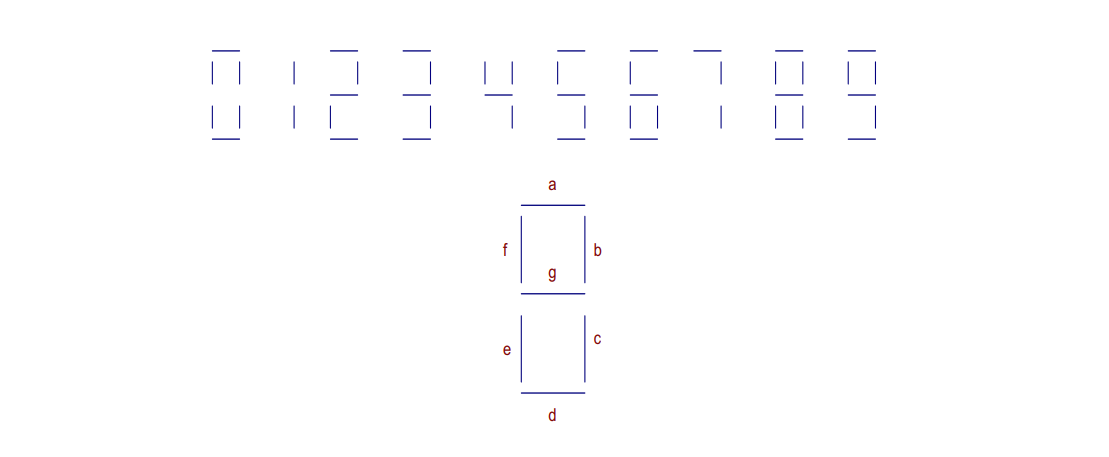
\includegraphics[width=0.4\linewidth]{7seg.png}
\end{figure}

\textit{Si vuole pilotare il segmento centrale ($g$) di un display a 7 segmenti a partire dalla cifra BCD in ingresso $a,b,c,d$. Il segmento centrale è spento solo per le cifre 0, 1 e 7.}

\medskip
\noindent Si costruisce la tabella di verità del segmento (con $a\leftrightarrow$ bit più significativo, $d\leftrightarrow$ bit meno significativo) e si segnano come \textbf{don't care} ($\times$) le combinazioni che non corrispondono a nessuna cifra BCD (cioè da 10 a 15), in modo da poter scegliere il loro valore così da semplificare il circuito:

\begin{center}
\begin{tabular}{cccc|c}
\toprule
$a$&$b$&$c$&$d$ & $g$\\
\midrule
0&0&0&0 & 0\\
0&0&0&1 & 0\\
0&0&1&0 & 1\\
0&0&1&1 & 1\\
0&1&0&0 & 1\\
0&1&0&1 & 1\\
0&1&1&0 & 1\\
0&1&1&1 & 0\\
1&0&0&0 & 1\\
1&0&0&1 & 1\\
\multicolumn{4}{c|}{1010 -- 1111} & $\times\;\times\;\times\;\times\;\times\;\times$\\
\bottomrule
\end{tabular}
\end{center}

\noindent La 2\textsuperscript{a} forma canonica (POS) del segmento, prima della semplificazione, contiene i tre maxtermini delle cifre 0, 1 e 7:
\[
F(a,b,c,d)=(a+b+c+d)\cdot(a+b+c+\overline{d})\cdot(a+\overline{b}+\overline{c}+\overline{d})
\]

\noindent Riportando la funzione (con i don't care) sulla mappa di Karnaugh a 4 variabili $cd\backslash ab$ e scegliendo opportunamente il valore dei don't care, si semplifica notevolmente il circuito:

\begin{center}
\begin{tikzpicture}[scale=0.78]
\draw (0,0) grid (4,4);
\node[font=\small] at (0.5,4.35) {00};
\node[font=\small] at (1.5,4.35) {01};
\node[font=\small] at (2.5,4.35) {11};
\node[font=\small] at (3.5,4.35) {10};
\node[font=\small, anchor=east] at (-0.1,3.5) {00};
\node[font=\small, anchor=east] at (-0.1,2.5) {01};
\node[font=\small, anchor=east] at (-0.1,1.5) {11};
\node[font=\small, anchor=east] at (-0.1,0.5) {10};
\node[font=\small] at (-0.7,4.35) {$cd{\backslash}ab$};
% raggruppamenti
\draw[rounded corners, fill=orange!30, opacity=0.5, draw=orange, thick] (2.1,0.1) rectangle (3.9,3.9);
\draw[rounded corners, fill=blue!25, opacity=0.5, draw=blue, thick] (1.15,2.15) rectangle (2.85,3.85);
\draw[rounded corners, fill=green!30, opacity=0.5, draw=green!60!black, thick] (0.15,0.25) rectangle (0.85,1.85);
\draw[rounded corners, fill=green!30, opacity=0.5, draw=green!60!black, thick] (3.15,0.25) rectangle (3.85,1.85);
\draw[rounded corners, draw=violet, very thick, dashed] (0.08,0.08) rectangle (3.92,0.92);
\node at (0.5,3.5) {0}; \node at (1.5,3.5) {1}; \node at (2.5,3.5) {$\times$}; \node at (3.5,3.5) {1};
\node at (0.5,2.5) {0}; \node at (1.5,2.5) {1}; \node at (2.5,2.5) {$\times$}; \node at (3.5,2.5) {1};
\node at (0.5,1.5) {1}; \node at (1.5,1.5) {0}; \node at (2.5,1.5) {$\times$}; \node at (3.5,1.5) {$\times$};
\node at (0.5,0.5) {1}; \node at (1.5,0.5) {1}; \node at (2.5,0.5) {$\times$}; \node at (3.5,0.5) {$\times$};
\end{tikzpicture}
\end{center}

\noindent Scegliendo i don't care in modo da formare i raggruppamenti più grandi possibile:
\begin{itemize}[leftmargin=1.5em, itemsep=1pt]
    \item \textcolor{orange}{\textbf{arancio}}: le colonne $ab=11$ e $ab=10$ (tutte 1 o don't care) danno $a$;
    \item \textcolor{blue}{\textbf{blu}}: colonne $01,11$ e righe $00,01$ danno $b\,\overline{c}$;
    \item \textcolor{green!60!black}{\textbf{verde}}: colonne $00$ e $10$ (adiacenti attraverso il bordo) e righe $11,10$ danno $\overline{b}\,c$;
    \item \textcolor{violet}{\textbf{viola}} (tratteggiato): la riga $cd=10$ dà $c\,\overline{d}$.
\end{itemize}
L'espressione semplificata diventa:
\[
a+c\overline{d}+\overline{b}c+b\overline{c} = a+c\overline{d}+(b\oplus c)
\]
molto più corta e immediata da realizzare rispetto alla forma canonica di partenza.

\begin{definizione}{Don't care}
I \textbf{don't care} si scelgono in modo da semplificare il più possibile il circuito risultante.
\end{definizione}

% ======================================================================
% circuito half adder — ingressi correttamente biforcati
\section{Sommatori}

\subsection{Semi-sommatore (half adder)}

\noindent Un \textbf{semi-sommatore} (half adder) è un circuito combinatorio in grado di eseguire la somma di due singoli bit ($a_i$ e $b_i$). Esso produce due uscite: il bit di somma $\Sigma_i$ e il bit di riporto generato $C_{i+1}$ (carry out). L'equazione logica che descrive la somma è un'operazione XOR ($\Sigma_i = a_i \oplus b_i$), mentre il riporto è dato da un'operazione AND ($C_{i+1} = a_i \cdot b_i$). 
Il limite del semi-sommatore è che non prevede un ingresso per il riporto proveniente da uno stadio precedente, limitandone l'utilizzo al solo bit meno significativo di un'addizione su più bit.

\begin{center}
\begin{circuitikz}[scale=1.0, every node/.style={scale=1.0}]
% Porte
\node[xor port] (XH) at (0, 1.5) {};
\node[and port] (AH) at (0, 0) {};

% Nodi di ingresso (allineati dinamicamente alle porte per evitare linee storte)
\coordinate (Ain) at (-2.5, 0 |- XH.in 1);
\coordinate (Bin) at (-2.5, 0 |- XH.in 2);
\node[left] at (Ain) {$a_i$};
\node[left] at (Bin) {$b_i$};

% Connessioni principali
\draw (Ain) -- (XH.in 1);
\draw (Bin) -- (XH.in 2);

% Derivazioni (i pallini sono centrati dinamicamente sulla linea)
\coordinate (Atap) at (-1.8, 0 |- XH.in 1);
\coordinate (Btap) at (-1.1, 0 |- XH.in 2);

\draw (Atap) to[short, *-] (Atap |- AH.in 1) -- (AH.in 1);
\draw (Btap) to[short, *-] (Btap |- AH.in 2) -- (AH.in 2);

% Uscite
\draw (XH.out) -- ++(0.7,0) node[right]{$\Sigma_i$};
\draw (AH.out) -- ++(0.7,0) node[right]{$C_{i+1}$};

\end{circuitikz}
\end{center}

\noindent Tabella di verità del semi-sommatore:

\begin{center}
\begin{tabular}{cc|cc}
\toprule
$a_i$ & $b_i$ & $\Sigma_i$ & $C_{i+1}$\\
\midrule
0&0&0&0\\
0&1&1&0\\
1&0&1&0\\
1&1&0&1\\
\bottomrule
\end{tabular}
\end{center}

\subsection{Sommatore completo (full adder)}

\noindent Il \textbf{sommatore completo} (full adder) risolve il limite del semi-sommatore aggiungendo un terzo ingresso $C_i$ per il riporto proveniente da uno stadio precedente. L'uscita somma $\Sigma_i$ vale 1 se il numero di ingressi a 1 è dispari, mentre il riporto $C_{i+1}$ vale 1 se almeno due ingressi sono a 1.
\medskip

\noindent Il circuito può essere ottenuto combinando due semi-sommatori e una porta OR finale per i riporti, in modo da tenere conto di tutti gli addendi:

\begin{center}
\begin{circuitikz}[scale=1.0, every node/.style={scale=1.0}]
% Primo HA
\draw (0, 0.3) rectangle (2.5, 2.3);
\node at (1.25, 1.3) {HA 1};
\node[right] at (0, 1.8) {$a_i$};
\node[right] at (0, 0.8) {$b_i$};
\node[left] at (2.5, 1.8) {$\Sigma'_i$};
\node[left] at (2.5, 0.8) {$C'_i$};

% Secondo HA
\draw (4.5, 1.3) rectangle (7.0, 3.3);
\node at (5.75, 2.3) {HA 2};
\node[right] at (4.5, 2.8) {$C_i$};
\node[right] at (4.5, 1.8) {$\Sigma'_i$};
\node[left] at (7.0, 2.8) {$\Sigma_i$};
\node[left] at (7.0, 1.8) {$C''_i$};

% OR gate
\node[or port] (OR) at (9.5, 1.3) {};

% Connessioni primo HA
\draw (-1.5, 1.8) node[left] {$a_i$} -- (0, 1.8);
\draw (-1.5, 0.8) node[left] {$b_i$} -- (0, 0.8);

% Connessioni intermedie e Cin
\draw (2.5, 1.8) -- (4.5, 1.8); % Linea dritta, nessun gradino!
\draw (-1.5, 2.8) node[left] {$C_i$} -- (4.5, 2.8); % Linea dritta, nessun gradino!

% Connessioni Carry
\draw (2.5, 0.8) -- (8.2, 0.8) |- (OR.in 2);
\draw (7.0, 1.8) -- (8.2, 1.8) |- (OR.in 1);

% Uscite finali
\draw (7.0, 2.8) -- (10.5, 2.8) node[right] {$\Sigma_i$};
\draw (OR.out) -- (10.5, 1.3) node[right] {$C_{i+1}$};

\end{circuitikz}
\end{center}

\noindent Tabella di verità del sommatore completo (con $\Sigma_i'$, $C_{i+1}'$ uscite del primo HA):

\begin{center}
\begin{tabular}{ccc|ccc}
\toprule
$a_i$ & $b_i$ & $C_i$ & $\Sigma_i'$ & $\Sigma_i$ & $C_{i+1}$\\
\midrule
0&0&0&0&0&0\\
0&0&1&0&1&0\\
0&1&0&1&1&0\\
0&1&1&1&0&1\\
1&0&0&1&1&0\\
1&0&1&1&0&1\\
1&1&0&0&0&1\\
1&1&1&0&1&1\\
\bottomrule
\end{tabular}
\end{center}

\subsubsection*{Logica dietro la tabella di verità}

Le due uscite del full adder obbediscono a regole semplici che si ricavano direttamente dal significato fisico della somma binaria.

\begin{itemize}
    \item \textbf{Bit di somma $\Sigma_i$ — ``parità'' degli ingressi:}
    $\Sigma_i = 1$ ogni volta che il numero totale di ingressi a \textbf{1} è \emph{dispari} (uno solo oppure tutti e tre). Questo coincide esattamente con l'\textbf{XOR a tre vie}:
    \[
        \Sigma_i = a_i \oplus b_i \oplus C_i
    \]
    Si può verificare intuitivamente: $1+1+0 = 2_{10} = 10_2$, la cifra delle unità è \textbf{0}; $1+1+1 = 3_{10} = 11_2$, la cifra delle unità è \textbf{1}. In entrambi i casi conta solo la parità degli addendi.

    \item \textbf{Bit di riporto $C_{i+1}$ — ``maggioranza'' degli ingressi:}
    $C_{i+1} = 1$ ogni volta che \emph{almeno due} ingressi su tre sono a \textbf{1} (funzione di maggioranza). Algebricamente:
    \[
        C_{i+1} = a_i b_i + b_i C_i + a_i C_i
    \]
    Ogni termine rappresenta una coppia che, sommata, produce riporto ($1+1 \ge 2$).
\end{itemize}

Queste due formule — e quindi l'intera tabella — si ricavano senza dover enumerare tutti gli 8 casi: basta ricordare che $\Sigma_i$ conta la \emph{parità} e $C_{i+1}$ la \emph{maggioranza} dei tre bit in ingresso.

% ======================================================================
\chapter{Sommatori, complemento a 2 e codici}

\section{Esempio: sommatore a 4 bit}
\textit{(27 marzo 2026)}

Collegando in cascata 4 sommatori completi (Full Adder, FA) si ottiene un circuito per l'addizione a 4 bit, noto come \textbf{Ripple-Carry Adder} (sommatore a propagazione di riporto). Ogni stadio $i$ somma i bit $a_i$ e $b_i$ più il riporto dello stadio precedente ($C_i$), generando il bit di somma ($\Sigma_i$) e il nuovo riporto ($C_{i+1}$) per lo stadio successivo.

\begin{center}
\begin{circuitikz}[scale=0.72, every node/.style={scale=0.72}]
% 4 FA in cascata
\foreach \i/\xi in {0/0, 1/2.6, 2/5.2, 3/7.8}{
  \draw (\xi,0) rectangle (\xi+2.0, 1.8);
  \node at (\xi+1.0, 0.9) {FA};
}
% Ingressi a_i
\foreach \i/\xi/\lab in {0/0/$a_0$, 1/2.6/$a_1$, 2/5.2/$a_2$, 3/7.8/$a_3$}{
  \draw[-latex] (\xi+0.6, 2.4) -- (\xi+0.6, 1.8) node[midway,right,font=\small]{\lab};
}
% Ingressi b_i
\foreach \i/\xi/\lab in {0/0/$b_0$, 1/2.6/$b_1$, 2/5.2/$b_2$, 3/7.8/$b_3$}{
  \draw[-latex] (\xi+1.4, 2.4) -- (\xi+1.4, 1.8) node[midway,right,font=\small]{\lab};
}
% Carry chain: C0 entra da sinistra, C1..C4 si propagano
\draw[-latex] (-1.0, 0.9) -- (0, 0.9) node[midway,above,font=\small]{$C_0$};
\draw[-latex] (2.0,0.9) -- (2.6,0.9) node[midway,above,font=\small]{$C_1$};
\draw[-latex] (4.6,0.9) -- (5.2,0.9) node[midway,above,font=\small]{$C_2$};
\draw[-latex] (7.2,0.9) -- (7.8,0.9) node[midway,above,font=\small]{$C_3$};
\draw[-latex] (9.8,0.9) -- (10.5,0.9) node[right,font=\small]{$C_4$};
% Uscite Sigma
\foreach \i/\xi/\lab in {0/0/$\Sigma_0$, 1/2.6/$\Sigma_1$, 2/5.2/$\Sigma_2$, 3/7.8/$\Sigma_3$}{
  \draw[-latex] (\xi+1.0, 0) -- (\xi+1.0,-0.6) node[below,font=\small]{\lab};
}
% Freccia overflow su C4
\draw[-latex,color=teal] (10.5,0.9) -- ++(0.5,0.4) node[right,font=\small,color=teal]{\textbf{bit di overflow}};
\end{circuitikz}
\end{center}

\medskip
\textbf{Esempio rapido di calcolo:}\\
Proviamo a sommare $A = 0101_2$ ($5_{10}$) e $B = 0011_2$ ($3_{10}$), ponendo il riporto iniziale $C_0 = 0$:
\begin{itemize}
    \item \textbf{Stadio 0:} $a_0(1) + b_0(1) + C_0(0) = 2 \implies \Sigma_0 = 0$, riporto $C_1 = 1$.
    \item \textbf{Stadio 1:} $a_1(0) + b_1(1) + C_1(1) = 2 \implies \Sigma_1 = 0$, riporto $C_2 = 1$.
    \item \textbf{Stadio 2:} $a_2(1) + b_2(0) + C_2(1) = 2 \implies \Sigma_2 = 0$, riporto $C_3 = 1$.
    \item \textbf{Stadio 3:} $a_3(0) + b_3(0) + C_3(1) = 1 \implies \Sigma_3 = 1$, riporto $C_4 = 0$.
\end{itemize}
Risultato corretto: $\Sigma = 1000_2$ ($8_{10}$).

\begin{definizione}{Bit di overflow $C_4$}
\textbf{Bit di overflow} ($C_4$): è il bit di riporto finale in uscita dal blocco più significativo. Se stiamo eseguendo addizioni su numeri binari puri (senza segno) a 4 bit e otteniamo $C_4 = 1$, il risultato supera il valore massimo rappresentabile ($15_{10}$). In questo caso si è verificato un errore di overflow.
\end{definizione}

\textbf{Il problema del ritardo (Delay):}\\
Il principale limite prestazionale di questo circuito è che ogni blocco FA deve "aspettare" che il blocco precedente calcoli il suo riporto. Il segnale $C$ deve letteralmente "propagarsi" a cascata (ripple) da $C_0$ fino a $C_4$. 
\begin{itemize}
    \item Se una singola porta logica ha un tempo di ritardo $\Delta T$, ogni blocco Full Adder impiega circa $3\Delta T$ per generare il riporto.
    \item In un sommatore a $n$ bit, il tempo totale $\Delta t$ cresce in modo lineare:
    \[ \Delta t = n \cdot 3\Delta T \]
\end{itemize}

\textbf{Soluzione: i sommatori Carry Look-Ahead (CLA)}\\
Per eliminare questa latenza si utilizzano circuiti più avanzati (ad anticipo di riporto). Attraverso un'apposita rete logica parallela, questi circuiti capiscono "in anticipo" se i vari stadi andranno a \emph{generare} o \emph{propagare} un riporto. In questo modo si possono calcolare tutte le uscite simultaneamente, con un ritardo bassissimo e logaritmico (o indipendente) rispetto alla lunghezza $n$ della parola.

\section{Modularità e Design Gerarchico}

Nella progettazione digitale moderna, si sfrutta ampiamente il concetto di \textbf{modularità}.

\begin{definizione}{Design Modulare}
un approccio in cui il sistema complesso viene suddiviso in sottomoduli standard e interscambiabili (es. usare i Full Adder base per costruire un sommatore a $n$ bit). Questi moduli possono essere aggiunti, rimossi o sostituiti senza dover alterare o riprogettare il resto del sistema.
\end{definizione}

\noindent I vantaggi principali includono:
\begin{itemize}
    \item \textbf{Astrazione}: chi progetta un processore non deve preoccuparsi della logica a porte interne al singolo FA, ma ne considera solo gli ingressi e le uscite.
    \item \textbf{Riutilizzo e Semplificazione}: un modulo testato e verificato può essere riutilizzato in più punti, rendendo il collaudo molto più affidabile.
\end{itemize}

\section{Sottrattori e numeri negativi}
\textit{(27 marzo 2026 -- cont.)}

Nei circuiti digitali, per rappresentare anche i numeri negativi, si deve "sacrificare" un bit (di solito il più significativo) per indicare il segno. Esistono diverse tecniche per farlo:

\textbf{1. Modulo e Segno}\\
Il bit più a sinistra indica il segno ($0$ = positivo, $1$ = negativo), mentre i restanti bit indicano il valore assoluto. Questa tecnica presenta un problema pratico: lo zero ha due rappresentazioni diverse. Ad esempio su 4 bit, $0000$ ($+0$) e $1000$ ($-0$) indicano entrambi il numero zero. Questo complica inutilmente i circuiti di calcolo.

\textbf{2. La teoria dei Complementi}\\
Per risolvere questo problema si utilizza un metodo matematico chiamato \emph{complemento}. Dato un numero $N$ espresso in una certa base $r$ e lungo $n$ cifre, si definiscono due tipi di complemento:
\begin{itemize}
    \item \textbf{Complemento alla base diminuita (base $r-1$):} \\
    Si definisce come $C_{r-1}(N) = (r^n - 1) - N$. Poiché $r^n - 1$ è il numero massimo rappresentabile ($N_{\max}$), si ottiene sottraendo il numero $N$ dal valore massimo.
    \item \textbf{Complemento alla base (base $r$):} \\
    Si definisce come $C_r(N) = r^n - N$. Essendo $r^n = (r^n - 1) + 1$, equivale matematicamente ad aggiungere $1$ al complemento alla base diminuita.
\end{itemize}

\textbf{Applicazione al Sistema Binario (Base 2):}\\
Nei sistemi binari (base $r=2$), queste due definizioni prendono il nome di \textbf{Complemento a 1} e \textbf{Complemento a 2}.

\textbf{Complemento a 1 ($C_1$):}
\[ C_1(N) = (2^n - 1) - N \]
Poiché $2^n-1$ è un numero composto da tutti "1" (es. $1111_2$), sottrarre $N$ significa banalmente \emph{invertire tutti i singoli bit} di $N$ (ogni bit $N_i$ diventa $\overline{N}_i$):
\[ C_1(N) = \overline{N}_{n-1}\cdots\overline{N}_1\overline{N}_0 \]

\textbf{Complemento a 2 ($C_2$):}
\[ C_2(N) = 2^n - N \]
Come visto prima, possiamo riscriverlo come $(2^n - 1 - N) + 1$. Questo significa che per calcolare il complemento a 2 basta prendere il complemento a 1 e sommare 1:
\[ C_2(N) = C_1(N) + 1 = \overline{N}_{n-1}\cdots\overline{N}_1\overline{N}_0 + 1 \]

\noindent\textit{Proprietà fondamentale:} Applicare due volte il complemento a 2 restituisce il numero originale, ovvero $C_2(C_2(N)) = N$.

\begin{definizione}{Complemento a 2}
Il \textbf{complemento a 2} è la notazione standard per rappresentare numeri interi con segno nei calcolatori. A differenza della codifica a modulo e segno, garantisce un'unica rappresentazione per lo zero (es. $0000$) e permette di eseguire somme e sottrazioni con la stessa rete logica hardware.
\end{definizione}

\noindent\textbf{Regola pratica per calcolare il complemento a 2 di un numero}:
\begin{enumerate}
    \item Si parte dal numero binario positivo (es. $+3_{10} = 0011_2$).
    \item Si invertono tutti i bit (complemento a 1): $0011 \to 1100$.
    \item Si somma $1$ al risultato: $1100 + 1 = 1101$. 
\end{enumerate}
Quindi $-3_{10} = 1101_2$ in complemento a 2 su 4 bit.

\medskip
Se verifichiamo calcolando l'addizione $-3 + 3$, avremo: $1101 + 0011 = 1\,0000$. Poiché lavoriamo a 4 bit, l'uno più a sinistra (il \emph{carry out} uscente) cade fuori dalla dimensione dei registri e viene ignorato. Il risultato memorizzato è esattamente $0000$, ovvero 0.

\subsection{Circuito sommatore/sottrattore a 4 bit}

Un grande vantaggio della codifica in complemento a 2 è la possibilità di eseguire sia addizioni che sottrazioni utilizzando il \textbf{medesimo circuito hardware}. Per farlo, si estende il classico sommatore (ripple-carry adder) introducendo delle porte logiche XOR sugli ingressi del secondo operando e sfruttando il riporto iniziale $C_0$ come segnale di controllo (selettore d'operazione).

\begin{center}
\begin{circuitikz}[scale=0.9, every node/.style={scale=0.9}]
\tikzset{FA/.style={draw, minimum width=1.6cm, minimum height=1.6cm, align=center}}

% Disegno dei 4 blocchi Full Adder
\foreach \i/\x in {0/0, 1/3.5, 2/7.0, 3/10.5} {
    \node[FA] (FA\i) at (\x,0) {FA$_\i$};
}

% Linea comune per C0 (selezione operazione)
\coordinate (C0line) at (-1.5, 4.0);
\draw (-1.5, 4.0) node[left] {$C_0$ (\textsf{0}=Add, \textsf{1}=Sub)} -- (11.0, 4.0);

% Connessione C0 come riporto in ingresso del primo FA
\draw[-latex] (-1.5, 4.0) -- (-1.5, 0) -- (FA0.west) node[midway, above] {$C_0$};

\foreach \i in {0,1,2,3} {
    % a_i input
    \draw[-latex] (FA\i.120 |- 0, 4.8) node[above] {$a_\i$} -- (FA\i.120);
    
    % b_i input e XOR
    \node[xor port, rotate=-90, scale=0.7] (XOR\i) at (FA\i.60 |- 0, 2.5) {};
    \draw[-latex] (XOR\i.out) -- (FA\i.60);
    
    % Connessione di b_i all'ingresso 1 dello XOR
    \draw (XOR\i.in 1) -- (XOR\i.in 1 |- 0, 4.8) node[above] {$b_\i$};
    
    % Connessione di C0 all'ingresso 2 dello XOR
    \draw (XOR\i.in 2) -- (XOR\i.in 2 |- C0line) node[circle, fill, inner sep=1.2pt] {};
}

% Carry chain tra i FA
\draw[-latex] (FA0.east) -- (FA1.west) node[midway, above] {$C_1$};
\draw[-latex] (FA1.east) -- (FA2.west) node[midway, above] {$C_2$};
\draw[-latex] (FA2.east) -- (FA3.west) node[midway, above] {$C_3$};

% Uscita C4
\draw[-latex] (FA3.east) -- ++(1.5,0) coordinate (C4out) node[above] {$C_4$};

% Uscite Somma (Sigma)
\foreach \i in {0,1,2,3} {
    \draw[-latex] (FA\i.south) -- ++(0,-1.0) node[below] {$\Sigma_\i$};
}

% XOR finale per l'overflow (E)
\node[xor port, scale=0.8] (E_XOR) at (13.5, -2.0) {};

% Preleviamo C3
\coordinate (tapC3) at (8.75, 0);
\draw (tapC3) node[circle, fill, inner sep=1.2pt] {} |- (E_XOR.in 2);

% Preleviamo C4
\coordinate (tapC4) at (12.0, 0);
\draw (tapC4) node[circle, fill, inner sep=1.2pt] {} |- (E_XOR.in 1);

\draw[-latex] (E_XOR.out) -- ++(0.8,0) node[right] {$E_{Overf}$};

\end{circuitikz}
\end{center}

Il funzionamento del circuito dipende dal valore del segnale di controllo $C_0$:

\begin{itemize}[leftmargin=1.5em]
    \item \textbf{Se $C_0=0$ (Addizione)}: la porta XOR riceve uno 0 e si comporta come un buffer trasparente ($b_i \oplus 0 = b_i$). Inoltre, il riporto in ingresso al primo FA è anch'esso 0. Il circuito esegue quindi una normale addizione: $S = a + b$.
    
    \item \textbf{Se $C_0=1$ (Sottrazione)}: la porta XOR riceve un 1 e si comporta come un invertitore logico ($b_i \oplus 1 = \overline{b}_i$), calcolando il complemento a 1 di $b$. Il riporto in ingresso al primo FA fornisce un ulteriore $+1$. In questo modo, il circuito calcola internamente l'espressione $a + \overline{b} + 1$. Poiché $\overline{b} + 1$ equivale a $-b$ (in complemento a 2), l'operazione totale svolta è esattamente la sottrazione: $S = a - b$.
    
    \item \textbf{Errore di Overflow ($E$)}: lavorando con un numero fisso di bit (in questo caso 4 bit, intervallo rappresentabile da $-8$ a $+7$), può accadere che il risultato reale dell'operazione sia al di fuori di questo intervallo. Questo errore prende il nome di \emph{overflow} e viene segnalato tramite una porta XOR applicata agli ultimi due riporti generati ($E = C_3 \oplus C_4$). Se $E=1$, si ha un \emph{overflow} e il risultato non è valido.
\end{itemize}

In generale, lavorando in complemento a 2 con 4 bit, si rappresenta l'intervallo da $-8$ a $+7$:
\begin{itemize}[leftmargin=1.5em]
    \item[\small$\blacksquare$] Se $\Sigma_3 = 0 \;\Leftrightarrow\;$ il risultato $\Sigma$ è positivo o nullo.
    \item[\small$\blacksquare$] Se $\Sigma_3 = 1 \;\Leftrightarrow\;$ il risultato $\Sigma$ è negativo.
\end{itemize}
Queste due regole valgono solo in assenza di overflow ($E=0$). Il segnale $E=C_3\oplus C_4$ ha senso per i numeri \emph{con segno}. Per una somma di numeri senza segno ($C_0=0$, intervallo $[0,15]$) l'overflow è segnalato direttamente da $C_4=1$.

\begin{center}
\begin{tikzpicture}[scale=1.1]
% Cerchio complemento a 2 a 4 bit
\draw (0,0) circle (2.0cm);
\foreach \angle/\val/\bin in {
  90/0/0000, 67.5/1/0001, 45/2/0010, 22.5/3/0011,
  0/4/0100, -22.5/5/0101, -45/6/0110, -67.5/7/0111,
  -90/-8/1000, -112.5/-7/1001, -135/-6/1010, -157.5/-5/1011,
  180/-4/1100, 157.5/-3/1101, 135/-2/1110, 112.5/-1/1111
}{
  \node[font=\tiny] at ({2.4*cos(\angle)},{2.4*sin(\angle)}) {\val};
  \node[font=\tiny] at ({1.6*cos(\angle)},{1.6*sin(\angle)}) {\bin};
}
\node[font=\small\bfseries, align=center] at (0,0) {4-bit};
% assi cardinali
\foreach \a in {0,90,180,270}{
  \draw[gray,thin] ({1.9*cos(\a)},{1.9*sin(\a)}) -- ({2.1*cos(\a)},{2.1*sin(\a)});
}
\end{tikzpicture}
\end{center}

% ======================================================================
\chapter{Codice Gray e ASCII}
\textit{(30 marzo 2026)}

\section{Codice Gray}

\begin{definizione}{Codice Gray}
Il \textbf{Codice Gray} è una codifica binaria non pesata in cui due valori consecutivi differiscono sempre e solo per \emph{un singolo bit}.
\end{definizione}

\noindent I vantaggi principali del codice Gray rispetto al normale codice binario puro sono:
\begin{itemize}[leftmargin=1.5em]
    \item \textbf{Prevenzione dei glitch (stati spuri)}: in un contatore binario normale, il passaggio ad esempio da $3$ ($011_2$) a $4$ ($100_2$) comporta la commutazione simultanea di 3 bit. Fisicamente, i bit non commuteranno mai nel medesimo istante esatto, causando passaggi in stati intermedi transitori errati (es. $011 \to 111 \to 100$). Con il codice Gray, cambiando un solo bit per ogni incremento, le transizioni sono sempre sicure e prive di glitch.
    \item \textbf{Riduzione della dissipazione di potenza}: in tecnologie CMOS, la potenza dinamica è dissipata principalmente durante le commutazioni di stato logico. Poiché nel codice Gray commuta sempre e solo un bit alla volta, la potenza dissipata è minima e costante nel tempo, rendendolo ideale per contatori a basso consumo o per le macchine a stati finiti.
\end{itemize}

\begin{minipage}[t]{0.30\linewidth}
\vspace{0pt}
\centering
\begin{tabular}{r c c}
\toprule
Dec. & Binario & Gray\\
\midrule
$0$  & $0000$ & $0000$ \\
$1$  & $0001$ & $0001$ \\
$2$  & $0010$ & $0011$ \\
$3$  & $0011$ & $0010$ \\
$4$  & $0100$ & $0110$ \\
$5$  & $0101$ & $0111$ \\
$6$  & $0110$ & $0101$ \\
$7$  & $0111$ & $0100$ \\
\midrule
$8$  & $1000$ & $1100$ \\
$9$  & $1001$ & $1101$ \\
$10$ & $1010$ & $1111$ \\
$11$ & $1011$ & $1110$ \\
$12$ & $1100$ & $1010$ \\
$13$ & $1101$ & $1011$ \\
$14$ & $1110$ & $1001$ \\
$15$ & $1111$ & $1000$ \\
\bottomrule
\end{tabular}
\end{minipage}%
\hfill
\begin{minipage}[t]{0.66\linewidth}
\vspace{0pt}
\noindent Dato un numero a $n$ bit (dove l'indice $n-1$ rappresenta il bit più significativo, MSB):

\medskip
\textbf{Conversione Binario $\to$ Gray}:\\
Il bit più significativo resta invariato. Ogni altro bit Gray si calcola come XOR tra il bit binario nella stessa posizione e il bit binario precedente (più significativo).
\[
G_{n-1} = B_{n-1} \qquad G_k = B_k \oplus B_{k+1} \quad \text{per } k < n-1
\]

\medskip
\textbf{Conversione Gray $\to$ Binario}:\\
Il bit più significativo resta invariato. Ogni altro bit binario si ottiene come XOR tra il bit Gray nella stessa posizione e il \emph{bit binario appena calcolato} nella posizione più significativa adiacente.
\[
B_{n-1} = G_{n-1} \qquad B_k = G_k \oplus B_{k+1} \quad \text{per } k < n-1
\]
\textit{(Nota matematica: sviluppando la ricorsione si nota che equivale alla formula $B_k = G_k \oplus G_{k+1} \oplus \dots \oplus G_{n-1}$, spesso implementata in hardware per velocizzare i tempi di calcolo parallelo).}
\end{minipage}

\subsection{Circuiti di conversione}

\begin{fitcenter}
\begin{circuitikz}[scale=0.85, every node/.style={scale=0.85}]

% ============================================================
% CIRCUITO BG  (Binario -> Gray)  —  colonna sinistra
% ============================================================
% G_{n-1} = B_{n-1} (passthrough), G_k = B_k XOR B_{k+1}

% Porte XOR per G0, G1, G2
\node[xor port] (BG0) at (2.0, 5.0) {};   % G0 = B0 XOR B1
\node[xor port] (BG1) at (2.0, 3.5) {};   % G1 = B1 XOR B2
\node[xor port] (BG2) at (2.0, 2.0) {};   % G2 = B2 XOR B3

% --- Ingresso B0 ---
\draw (-1.0, 0 |- BG0.in 1) node[left]{$B_0$} -- (BG0.in 1);

% --- Ingresso B1 ---
\draw (-1.0, 4.25) node[left]{$B_1$} -- (0.0, 4.25);
\node[circle, fill, inner sep=1.5pt] at (0.0, 4.25) {};
\draw (0.0, 4.25) |- (BG0.in 2);
\draw (0.0, 4.25) |- (BG1.in 1);

% --- Ingresso B2 ---
\draw (-1.0, 2.75) node[left]{$B_2$} -- (0.2, 2.75);
\node[circle, fill, inner sep=1.5pt] at (0.2, 2.75) {};
\draw (0.2, 2.75) |- (BG1.in 2);
\draw (0.2, 2.75) |- (BG2.in 1);

% --- Ingresso B3 ---
\draw (-1.0, 1.0) node[left]{$B_3$} -- (4.3, 1.0) node[right]{$G_3$};
\node[circle, fill, inner sep=1.5pt] at (0.4, 1.0) {};
\draw (0.4, 1.0) |- (BG2.in 2);

% --- Uscite Gray ---
\draw (BG0.out) -- (4.3, 0 |- BG0.out) node[right]{$G_0$};
\draw (BG1.out) -- (4.3, 0 |- BG1.out) node[right]{$G_1$};
\draw (BG2.out) -- (4.3, 0 |- BG2.out) node[right]{$G_2$};

\node[below, font=\small\bfseries, color=teal] at (2.0, 0.4) {Conversione B$\to$G};

% ============================================================
% CIRCUITO GB  (Gray -> Binario)  —  colonna destra
% ============================================================
% B_{n-1} = G_{n-1}, poi B_k = G_k XOR B_{k+1}

% Porte XOR per B0, B1, B2
\node[xor port] (GB0) at (9.5, 5.0) {};   % B0 = G0 XOR B1
\node[xor port] (GB1) at (9.5, 3.5) {};   % B1 = G1 XOR B2
\node[xor port] (GB2) at (9.5, 2.0) {};   % B2 = G2 XOR B3

% --- Ingresso G0 ---
\draw (6.5, 0 |- GB0.in 1) node[left]{$G_0$} -- (GB0.in 1);

% --- Ingresso G1 ---
\draw (6.5, 0 |- GB1.in 1) node[left]{$G_1$} -- (GB1.in 1);

% --- Ingresso G2 ---
\draw (6.5, 0 |- GB2.in 1) node[left]{$G_2$} -- (GB2.in 1);

% --- Ingresso G3 e Uscita B3 (passthrough) ---
\draw (6.5, 1.0) node[left]{$G_3$} -- (11.8, 1.0) node[right]{$B_3$};

% --- Uscita B0 ---
\draw (GB0.out) -- (11.8, 0 |- GB0.out) node[right]{$B_0$};

% --- Uscita B1 e feedback ---
\draw (GB1.out) -- (11.8, 0 |- GB1.out) node[right]{$B_1$};
\node[circle, fill, inner sep=1.5pt] at (10.5, 0 |- GB1.out) {};
\draw (10.5, 0 |- GB1.out) -- (10.5, 4.25) -- (7.5, 4.25) |- (GB0.in 2);

% --- Uscita B2 e feedback ---
\draw (GB2.out) -- (11.8, 0 |- GB2.out) node[right]{$B_2$};
\node[circle, fill, inner sep=1.5pt] at (10.7, 0 |- GB2.out) {};
\draw (10.7, 0 |- GB2.out) -- (10.7, 2.75) -- (7.7, 2.75) |- (GB1.in 2);

% --- Feedback da B3 ---
\node[circle, fill, inner sep=1.5pt] at (10.9, 1.0) {};
\draw (10.9, 1.0) -- (10.9, 1.35) -- (7.9, 1.35) |- (GB2.in 2);

\node[below, font=\small\bfseries, color=teal] at (9.5, 0.4) {Conversione G$\to$B};

\end{circuitikz}
\end{fitcenter}

% ======================================================================
\subsection{Esercizi svolti: conversioni passo-passo}

Applichiamo le formule ai due casi classici usando numeri a \textbf{4 bit}
($B_3 B_2 B_1 B_0$, con $B_3$ = MSB).

% ------------------------------------------------------------------
\subsubsection*{Esercizio 1 — Binario $\to$ Gray: \quad $1011_2 \;(=11_{10})$}

La regola è: $G_3 = B_3$, poi $G_k = B_k \oplus B_{k+1}$.

\medskip
\begin{center}
\begin{tabular}{c|c|c|l}
\toprule
Bit & Formula & Calcolo & Risultato\\
\midrule
$G_3$ & $B_3$ & $1$ & $G_3 = \mathbf{1}$ \\
$G_2$ & $B_2 \oplus B_3$ & $0 \oplus 1$ & $G_2 = \mathbf{1}$ \\
$G_1$ & $B_1 \oplus B_2$ & $1 \oplus 0$ & $G_1 = \mathbf{1}$ \\
$G_0$ & $B_0 \oplus B_1$ & $1 \oplus 1$ & $G_0 = \mathbf{0}$ \\
\bottomrule
\end{tabular}
\end{center}

\medskip
\noindent Si parte dal MSB e si scende verso il LSB, applicando uno XOR bit a bit con il vicino più significativo già noto:

\[
\underbrace{1}_{B_3}\;\underbrace{0}_{B_2}\;\underbrace{1}_{B_1}\;\underbrace{1}_{B_0}
\;\xrightarrow{\text{B}\to\text{G}}\;
\underbrace{1}_{G_3}\;\underbrace{1}_{G_2}\;\underbrace{1}_{G_1}\;\underbrace{0}_{G_0}
\quad\Rightarrow\quad \boxed{1110_G}
\]

\vspace{1.5em}

% ------------------------------------------------------------------
\subsubsection*{Esercizio 2 — Gray $\to$ Binario: \quad $1110_G$}

La regola è: $B_3 = G_3$, poi $B_k = G_k \oplus B_{k+1}$ (si usa il binario \emph{già calcolato} al passo precedente, non il Gray).

\medskip
\begin{center}
\begin{tabular}{c|c|c|l}
\toprule
Bit & Formula & Calcolo & Risultato\\
\midrule
$B_3$ & $G_3$ & $1$ & $B_3 = \mathbf{1}$ \\
$B_2$ & $G_2 \oplus B_3$ & $1 \oplus 1$ & $B_2 = \mathbf{0}$ \\
$B_1$ & $G_1 \oplus B_2$ & $1 \oplus 0$ & $B_1 = \mathbf{1}$ \\
$B_0$ & $G_0 \oplus B_1$ & $0 \oplus 1$ & $B_0 = \mathbf{1}$ \\
\bottomrule
\end{tabular}
\end{center}

\medskip
\noindent Anche qui si procede dall'MSB verso l'LSB, ma ogni XOR usa il \emph{bit binario appena ricavato} (non il Gray):

\[
\underbrace{1}_{G_3}\;\underbrace{1}_{G_2}\;\underbrace{1}_{G_1}\;\underbrace{0}_{G_0}
\;\xrightarrow{\text{G}\to\text{B}}\;
\underbrace{1}_{B_3}\;\underbrace{0}_{B_2}\;\underbrace{1}_{B_1}\;\underbrace{1}_{B_0}
\quad\Rightarrow\quad \boxed{1011_2 = 11_{10}}
\]

\vspace{0.5em}
\noindent\textit{I due esercizi si invertono a vicenda: il risultato di Esercizio~2 coincide esattamente con il punto di partenza di Esercizio~1, confermando la correttezza delle due conversioni.}

\vspace{1.5em}

% ------------------------------------------------------------------
\subsubsection*{Esercizio 3 — Binario $\to$ Gray: \quad $1101_2 \;(=13_{10})$}

\medskip
\begin{center}
\begin{tabular}{c|c|c|l}
\toprule
Bit & Formula & Calcolo & Risultato\\
\midrule
$G_3$ & $B_3$ & $1$ & $G_3 = \mathbf{1}$ \\
$G_2$ & $B_2 \oplus B_3$ & $1 \oplus 1$ & $G_2 = \mathbf{0}$ \\
$G_1$ & $B_1 \oplus B_2$ & $0 \oplus 1$ & $G_1 = \mathbf{1}$ \\
$G_0$ & $B_0 \oplus B_1$ & $1 \oplus 0$ & $G_0 = \mathbf{1}$ \\
\bottomrule
\end{tabular}
\end{center}

\[
1101_2 \;\xrightarrow{\text{B}\to\text{G}}\; \boxed{1011_G}
\]

\subsubsection*{Esercizio 4 — Gray $\to$ Binario: \quad $1011_G$}

\medskip
\begin{center}
\begin{tabular}{c|c|c|l}
\toprule
Bit & Formula & Calcolo & Risultato\\
\midrule
$B_3$ & $G_3$ & $1$ & $B_3 = \mathbf{1}$ \\
$B_2$ & $G_2 \oplus B_3$ & $0 \oplus 1$ & $B_2 = \mathbf{1}$ \\
$B_1$ & $G_1 \oplus B_2$ & $1 \oplus 1$ & $B_1 = \mathbf{0}$ \\
$B_0$ & $G_0 \oplus B_1$ & $1 \oplus 0$ & $B_0 = \mathbf{1}$ \\
\bottomrule
\end{tabular}
\end{center}

\[
1011_G \;\xrightarrow{\text{G}\to\text{B}}\; \boxed{1101_2 = 13_{10}}
\]

\vspace{0.5em}
\noindent\textit{Anche qui la coppia Esercizio~3 e Esercizio~4 è inversa, come atteso.}


% ======================================================================
\section{Codice ASCII}
 
\begin{definizione}{ASCII}
L'\textbf{ASCII} (\emph{American Standard Code for Information Interchange}) è il sistema di codifica standard utilizzato storicamente per rappresentare caratteri alfanumerici e simboli di controllo nei dispositivi digitali e di telecomunicazione.
\end{definizione}
 
La tabella ASCII standard originale utilizza \textbf{7 bit} per codificare 128 simboli diversi ($2^7 = 128$). I codici sono suddivisi logicamente in:
\begin{itemize}[leftmargin=1.5em]
    \item \textbf{0--31 e 127}: \emph{Caratteri di controllo} (non stampabili), usati originariamente per gestire la formattazione hardware delle telescriventi (es. ritorno a capo \texttt{CR}, avanzamento riga \texttt{LF}, tabulazione \texttt{HT}) o il protocollo di comunicazione.
    \item \textbf{32--47, 58--64, 91--96, 123--126}: \emph{Simboli grafici e punteggiatura} (lo spazio è il primo carattere stampabile, codice decimale 32).
    \item \textbf{48--57}: \emph{Cifre numeriche} (da '0' a '9').
    \item \textbf{65--90}: \emph{Lettere maiuscole} (da 'A' a 'Z').
    \item \textbf{97--122}: \emph{Lettere minuscole} (da 'a' a 'z').
\end{itemize}

\noindent \textbf{Proprietà notevole}: le lettere maiuscole e le rispettive minuscole differiscono sempre esattamente per \emph{un solo bit}: il bit di peso $2^5=32$ (bit numero 5 contando da 0, cioè il sesto da destra).
Ad esempio, la 'A' vale $65_{10}$ ($01\textbf{0}00001_2$) e la 'a' vale $97_{10}$ ($01\textbf{1}00001_2$). Questa ingegnosa scelta progettuale non è casuale: permette ai sistemi digitali e ai microprocessori di convertire istantaneamente e a basso costo computazionale i caratteri dal maiuscolo al minuscolo semplicemente agendo su quel bit con una maschera logica (lo XOR con $0010\,0000_2$ scambia maiuscole e minuscole; l'OR forza la minuscola).

\medskip
 
\begin{fitcenter}
{\footnotesize\setlength{\tabcolsep}{3pt}%
\begin{tabular}{@{}c|c|c|c@{\hspace{6pt}}c|c|c|c@{\hspace{6pt}}c|c|c|c@{\hspace{6pt}}c|c|c|c@{}}
\textbf{Dec} & \textbf{Oct} & \textbf{Hex} & \textbf{Char} & \textbf{Dec} & \textbf{Oct} & \textbf{Hex} & \textbf{Char} & \textbf{Dec} & \textbf{Oct} & \textbf{Hex} & \textbf{Char} & \textbf{Dec} & \textbf{Oct} & \textbf{Hex} & \textbf{Char}\\
\hline
0&000&00&NUL & 32&040&20&(sp) & 64&100&40&@ & 96&140&60&\textasciigrave\\
1&001&01&SOH & 33&041&21&! & 65&101&41&A & 97&141&61&a\\
2&002&02&STX & 34&042&22&\textquotedbl & 66&102&42&B & 98&142&62&b\\
3&003&03&ETX & 35&043&23&\# & 67&103&43&C & 99&143&63&c\\
4&004&04&EOT & 36&044&24&\$ & 68&104&44&D & 100&144&64&d\\
5&005&05&ENQ & 37&045&25&\% & 69&105&45&E & 101&145&65&e\\
6&006&06&ACK & 38&046&26&\& & 70&106&46&F & 102&146&66&f\\
7&007&07&BEL & 39&047&27&\textquotesingle & 71&107&47&G & 103&147&67&g\\
8&010&08&BS & 40&050&28&( & 72&110&48&H & 104&150&68&h\\
9&011&09&HT & 41&051&29&) & 73&111&49&I & 105&151&69&i\\
10&012&0A&LF & 42&052&2A&* & 74&112&4A&J & 106&152&6A&j\\
11&013&0B&VT & 43&053&2B&+ & 75&113&4B&K & 107&153&6B&k\\
12&014&0C&FF & 44&054&2C&, & 76&114&4C&L & 108&154&6C&l\\
13&015&0D&CR & 45&055&2D&- & 77&115&4D&M & 109&155&6D&m\\
14&016&0E&SO & 46&056&2E&. & 78&116&4E&N & 110&156&6E&n\\
15&017&0F&SI & 47&057&2F&/ & 79&117&4F&O & 111&157&6F&o\\
16&020&10&DLE & 48&060&30&0 & 80&120&50&P & 112&160&70&p\\
17&021&11&DC1 & 49&061&31&1 & 81&121&51&Q & 113&161&71&q\\
18&022&12&DC2 & 50&062&32&2 & 82&122&52&R & 114&162&72&r\\
19&023&13&DC3 & 51&063&33&3 & 83&123&53&S & 115&163&73&s\\
20&024&14&DC4 & 52&064&34&4 & 84&124&54&T & 116&164&74&t\\
21&025&15&NAK & 53&065&35&5 & 85&125&55&U & 117&165&75&u\\
22&026&16&SYN & 54&066&36&6 & 86&126&56&V & 118&166&76&v\\
23&027&17&ETB & 55&067&37&7 & 87&127&57&W & 119&167&77&w\\
24&030&18&CAN & 56&070&38&8 & 88&130&58&X & 120&170&78&x\\
25&031&19&EM & 57&071&39&9 & 89&131&59&Y & 121&171&79&y\\
26&032&1A&SUB & 58&072&3A&: & 90&132&5A&Z & 122&172&7A&z\\
27&033&1B&ESC & 59&073&3B&; & 91&133&5B&[ & 123&173&7B&\{\\
28&034&1C&FS & 60&074&3C&\textless & 92&134&5C&\textbackslash & 124&174&7C&\textbar\\
29&035&1D&GS & 61&075&3D&= & 93&135&5D&] & 125&175&7D&\}\\
30&036&1E&RS & 62&076&3E&\textgreater & 94&136&5E&\textasciicircum & 126&176&7E&\textasciitilde\\
31&037&1F&US & 63&077&3F&? & 95&137&5F&\_ & 127&177&7F&DEL\\
\hline
\end{tabular}%
}
\end{fitcenter}
 
\begin{sloppypar}
\noindent\textit{Legenda}: le colonne da sinistra a destra mostrano decimale, ottale, esadecimale e il carattere corrispondente. I caratteri di controllo (0--31 e 127) sono abbreviati (es.\ NUL=null, SOH=start of heading, CR=carriage return, DEL=delete, ecc.).
\end{sloppypar}
 
\begin{important}
\noindent\textbf{Intervalli notevoli}:
\begin{itemize}[leftmargin=1.3em]
    \item Caratteri di controllo: 0--31 e 127;
    \item Spazio: 32;
    \item Caratteri stampabili: 33--126;
    \item Cifre: 48--57 (0--9);
    \item Lettere maiuscole: 65--90 (A--Z);
    \item Lettere minuscole: 97--122 (a--z).
\end{itemize}
\end{important}

% ======================================================================
\chapter{Logica sequenziale}

\section{Circuiti combinatori e circuiti sequenziali}

Finora abbiamo visto circuiti in cui l'output dipende esclusivamente dagli input: \textbf{circuiti combinatori}.

\medskip
\noindent Esistono anche circuiti in cui lo stato delle uscite dipende anche dallo stato in cui il circuito era in precedenza: questi circuiti seguono una \textbf{logica sequenziale}.

\medskip
\noindent Nei circuiti sequenziali è necessario che ci sia una \textbf{memoria}, un feedback.

\begin{center}
\begin{circuitikz}[scale=0.85, every node/.style={scale=0.85}]
% --- Circuito combinatorio ---
\draw (0,0) rectangle (2.2,2.0);
\node at (1.1,1.0) {CC};
\foreach \y in {1.6,1.0,0.4}{
  \draw[-latex] (-1.0,\y) -- (0,\y);
}
\node[left] at (-1.0,1.0) {$I_i$};
\foreach \y in {1.6,1.0,0.4}{
  \draw[-latex] (2.2,\y) -- (3.2,\y);
}
\node[right] at (3.2,1.0) {$O_i$};
\node[below, font=\small, color=teal] at (1.1,-0.5) {logica combinatoria};
\node[below] at (1.1,-1.0) {$O_i(t)=f\big(I_i(t)\big)$};

% --- Circuito sequenziale ---
\begin{scope}[xshift=7cm]
\draw (0,0) rectangle (2.2,2.0);
\node at (1.1,1.0) {CS};
\foreach \y in {1.6,1.0,0.4}{
  \draw[-latex] (-1.0,\y) -- (0,\y);
}
\node[left] at (-1.0,1.0) {$I_i$};
\foreach \y in {1.6,1.0,0.4}{
  \draw[-latex] (2.2,\y) -- (3.2,\y);
}
\node[right] at (3.2,1.0) {$O_i$};
% feedback loop
\draw (3.0,1.6) -- (3.6,1.6) -- (3.6,-0.6) -- (-0.6,-0.6) -- (-0.6,0.4) -- (0,0.4);
\node[right, font=\scriptsize] at (3.65,1.6) {tratti di feedback};
\node[below, font=\small, color=teal] at (1.1,-1.0) {logica sequenziale};
\node[below] at (1.1,-1.5) {$O_i(t+\Delta t)=f\big(I_i(t),O_i(t)\big)$};
\end{scope}
\end{circuitikz}
\end{center}

\section{Bistabilità e oscillazione}

Il \textbf{circuito bistabile} rappresenta la forma più semplice di \textbf{memoria} in elettronica digitale. Si ottiene collegando in anello chiuso un numero \textbf{pari} di porte logiche invertenti (ad esempio porte NOT). Poiché ogni segnale viene invertito due volte, il valore che ritorna all'ingresso è uguale a quello di partenza. Questo crea un \textbf{feedback positivo} che rinforza e mantiene stabile all'infinito lo stato logico assunto all'accensione, conservando così un bit di informazione ($0$ o $1$).

\begin{important}
Il problema di un semplice anello di porte NOT è che è un sistema isolato: \textbf{non è possibile modificarne lo stato} dall'esterno. Per potervi "scrivere" un nuovo bit (impostarlo a 1 o azzerarlo a 0), le porte NOT vengono sostituite con porte \textbf{NOR} o \textbf{NAND}, le quali offrono dei terminali di ingresso aggiuntivi per i segnali di controllo.
\end{important}

Se invece colleghiamo in anello chiuso un numero \textbf{dispari} di porte NOT, otteniamo un \textbf{circuito oscillante} (o \emph{ring oscillator}). L'inversione dispari fa sì che il segnale ritorni all'ingresso invertito rispetto alla partenza. Questo genera una perenne instabilità: l'uscita continua a commutare ciclicamente tra $0$ e $1$, con un periodo $T$ proporzionale al numero di porte e al ritardo di propagazione di ciascuna di esse.

\begin{center}
\begin{circuitikz}[scale=0.9, every node/.style={scale=0.9}]
% NOT pari -> bistabile
\node[not port] (n1) at (0,0) {};
\node[not port] (n2) at (2.5,0) {};
\draw (n1.out) -- (n2.in);
\draw (n2.out) -- ++(0.4,0) coordinate (tapb) -- ++(0.6,0) node[right]{$Q$};
% Feedback superiore pulito
\node[circle, fill, inner sep=1.5pt] at (tapb) {};
\draw (tapb) -- ++(0, 1.2) -| (n1.in);

% Waveform output
\begin{scope}[yshift=-2.2cm, xshift=-0.25cm]
  \draw[->, >=stealth, gray] (0,0) -- (3.2,0) node[right, black, font=\scriptsize] {$t$};
  \draw[->, >=stealth, gray] (0,0) -- (0,1.2) node[above, black, font=\scriptsize] {$Q(t)$};
  \draw[thick, red] (0,0.8) -- (3.0,0.8) node[right, font=\scriptsize, color=red] {costante (1)};
  \draw[thick, red, dashed, opacity=0.4] (0,0.2) -- (3.0,0.2) node[right, font=\scriptsize, opacity=0.6, color=red] {costante (0)};
  \node[left, font=\tiny] at (0,0.8) {H};
  \node[left, font=\tiny] at (0,0.2) {L};
\end{scope}

\node[below, font=\small, color=teal] at (1.25,-2.8) {Circuito Bi-stabile (\# NOT pari)};
\end{circuitikz}
\hspace{1cm}
\begin{circuitikz}[scale=0.9, every node/.style={scale=0.9}]
% NOT dispari -> oscillante
\node[not port] (m1) at (0,0) {};
\node[not port] (m2) at (2.0,0) {};
\node[not port] (m3) at (4.0,0) {};
\draw (m1.out) -- (m2.in);
\draw (m2.out) -- (m3.in);
\draw (m3.out) -- ++(0.4,0) coordinate (tapo) -- ++(0.6,0) node[right]{$Q$};
% Feedback superiore pulito
\node[circle, fill, inner sep=1.5pt] at (tapo) {};
\draw (tapo) -- ++(0, 1.2) -| (m1.in);

% Waveform output
\begin{scope}[yshift=-2.2cm, xshift=0.3cm]
  \draw[->, >=stealth, gray] (0,0) -- (4.2,0) node[right, black, font=\scriptsize] {$t$};
  \draw[->, >=stealth, gray] (0,0) -- (0,1.2) node[above, black, font=\scriptsize] {$Q(t)$};
  \draw[thick, red] (0,0.8) -- (0.6,0.8) -- (0.6,0.2) -- (1.2,0.2) -- (1.2,0.8) -- (1.8,0.8) -- (1.8,0.2) -- (2.4,0.2) -- (2.4,0.8) -- (3.0,0.8) -- (3.0,0.2) -- (3.6,0.2) -- (3.6,0.8) -- (4.0,0.8) node[right, font=\scriptsize, color=red] {quadra};
  \node[left, font=\tiny] at (0,0.8) {H};
  \node[left, font=\tiny] at (0,0.2) {L};
\end{scope}

\node[below, font=\small, color=teal] at (2.2,-2.8) {Circuito Oscillante (\# NOT dispari)};
\end{circuitikz}
\end{center}

\section{Latch}

\begin{definizione}{Latch}
Il circuito di memoria fondamentale dell'elettronica digitale sequenziale, capace di conservare un bit e di essere aggiornato tramite appositi segnali di ingresso.
\end{definizione}

Il Latch più semplice (Latch SR, \emph{Set-Reset}) nasce dall'evoluzione del circuito bistabile: sostituendo le due porte NOT con due porte \textbf{NOR} (o NAND) e incrociando i collegamenti (\emph{cross-coupling}), otteniamo due ingressi di controllo: \textbf{S} (\emph{Set}) e \textbf{R} (\emph{Reset}).

\begin{center}
\begin{circuitikz}[scale=1.0, every node/.style={scale=1.0}]
\node[nor port] (G1) at (0,1.2) {};
\node[nor port] (G2) at (0,-1.2) {};

% Ingressi S e R
\draw (G1.in 1) -- ++(-1.2,0) node[left]{$R$};
\draw (G2.in 2) -- ++(-1.2,0) node[left]{$S$};

% Uscite Q e Q_not
\draw (G1.out) -- ++(0.4,0) coordinate (tap1) -- ++(1.0,0) node[right]{$Q$};
\draw (G2.out) -- ++(0.4,0) coordinate (tap2) -- ++(1.0,0) node[right]{$\overline{Q}$};

\node[circle, fill, inner sep=1.2pt] at (tap1) {};
\node[circle, fill, inner sep=1.2pt] at (tap2) {};

% Cross coupling diagonale
\draw (tap1) -- ($(G2.in 1)+(-0.4,0)$) -- (G2.in 1);
\draw (tap2) -- ($(G1.in 2)+(-0.4,0)$) -- (G1.in 2);

\node[below=1.0cm, font=\small, color=teal] at (0,-1.2) {Latch SR con porte NOR};
\end{circuitikz}
\end{center}

\noindent \textbf{Funzionamento e Tabella di verità del Latch SR con porte NOR}

\smallskip
\noindent Le uscite sono $Q$ e $\overline{Q}$. Il pedice $n$ indica lo stato \emph{attuale} del latch (prima che gli ingressi cambino), mentre $n{+}1$ indica il nuovo stato che il circuito assumerà.

\begin{center}
\renewcommand{\arraystretch}{1.35}
\begin{tabular}{>{{\centering}}m{0.8cm}>{{\centering}}m{0.8cm}|>{{\centering}}m{1.5cm}>{{\centering}}m{1.5cm}|l}
\toprule
$R$ & $S$ & $Q_{n+1}$ & $\overline{Q}_{n+1}$ & \textbf{Comportamento}\\
\midrule
$0$ & $0$ & $Q_n$ & $\overline{Q}_n$ & \textcolor{teal}{\textbf{MEMORIA}} (stato mantenuto)\\
$0$ & $1$ & $1$ & $0$ & \textcolor{teal}{\textbf{SET}} — forza $Q=1$\\
$1$ & $0$ & $0$ & $1$ & \textcolor{teal}{\textbf{RESET}} — forza $Q=0$\\
\rowcolor{red!8} $1$ & $1$ & $0$ & $0$ & \textcolor{red!70!black}{\textbf{PROIBITO} — $Q=\overline{Q}=0$, uscita incoerente}\\
\bottomrule
\end{tabular}
\end{center}

\noindent Di seguito viene spiegato il meccanismo fisico di ogni stato, seguendo il percorso del segnale attraverso le due porte NOR incrociate.

\begin{itemize}[leftmargin=1.5em, itemsep=4pt]

    \item \textcolor{teal}{\textbf{Memoria ($R=0,\;S=0$)}}\quad
    Con entrambi gli ingressi a $0$, ogni porta NOR ha un solo ingresso attivo: quello proveniente
    dall'uscita dell'altra porta (\emph{cross-coupling}). Il circuito si comporta esattamente come
    un anello di due invertitori: qualunque stato ($Q=0$ o $Q=1$) è auto-consistente e viene
    mantenuto indefinitamente. \textbf{Non avviene nessun cambiamento}: il bit memorizzato rimane
    intatto.

    \item \textcolor{teal}{\textbf{Set ($R=0,\;S=1$)}}\quad
    L'ingresso $S=1$ forza l'uscita della porta NOR inferiore a $0$
    ($\overline{Q}\to 0$), indipendentemente dal suo secondo ingresso di feedback.
    Questo $0$ si propaga alla porta NOR superiore, la quale ha ora \emph{entrambi} gli ingressi
    a $0$ ($R=0$ e il feedback $\overline{Q}=0$), quindi porta la sua uscita a
    $Q\to 1$. Il latch si \textbf{stabilizza} nello stato $Q=1$, $\overline{Q}=0$.

    \item \textcolor{teal}{\textbf{Reset ($R=1,\;S=0$)}}\quad
    Simmetrico al caso precedente: $R=1$ forza l'uscita della porta NOR superiore a $0$
    ($Q\to 0$). Questo $0$ raggiunge la porta NOR inferiore che, con entrambi gli ingressi
    a $0$ ($S=0$ e il feedback $Q=0$), porta $\overline{Q}\to 1$.
    Il latch si \textbf{stabilizza} nello stato $Q=0$, $\overline{Q}=1$.

    \item \textcolor{red!70!black}{\textbf{Stato proibito ($R=1,\;S=1$)}}\quad
    Con entrambi gli ingressi a $1$, \emph{entrambe} le porte NOR vengono forzate
    a $0$: $Q=0$ e $\overline{Q}=0$. Questo viola il requisito fondamentale del latch,
    ovvero che le uscite siano sempre complementari. Ancora più grave è ciò che accade
    se si riportano poi $R$ e $S$ a $0$ simultaneamente: entrambe le porte
    tenteranno di portare la propria uscita a $1$ nello stesso istante.
    Il risultato finale dipenderà da infinitesime differenze nei ritardi di propagazione
    e nelle caratteristiche costruttive dei transistor, rendendo l'uscita
    \textbf{imprevedibile} e potenzialmente causando una \emph{metastabilità} o
    un'oscillazione transitoria. Per questo motivo la combinazione $R=S=1$ è da
    evitare sempre.

\end{itemize}
% ======================================================================
% Continuazione pagina 6 (10/04/2026)
% ======================================================================

\subsection{Latch RS con NOR: funzione caratteristica}

\noindent In questa sezione ricaviamo \emph{algebricamente} l'equazione che governa il latch con porte NOR.
Il procedimento si basa sull'analisi del \textbf{circuito equivalente}, in cui l'anello di retroazione viene idealmente interrotto per studiare la propagazione dei segnali da un istante $t$ all'istante successivo $t+\Delta t$.

\medskip
\noindent\textbf{1. Costruzione dell'equazione dal circuito equivalente.}
Seguendo il percorso dei segnali nel circuito equivalente:
\begin{itemize}[leftmargin=1.5em]
    \item La prima porta NOR riceve come ingressi il segnale $S$ e lo stato attuale $Q(t)$ proveniente dalla retroazione. Il suo risultato è l'uscita complementata al tempo $t$, ovvero $\overline{Q}(t)$:
    \[ \overline{Q}(t) = \overline{S + Q(t)} \]
    \item La seconda porta NOR riceve l'ingresso $R$ e il segnale appena calcolato $\overline{Q}(t)$. Il suo risultato è il nuovo stato del latch, $Q(t+\Delta t)$:
    \[ Q(t+\Delta t) = \overline{ R + \overline{Q}(t) } \]
\end{itemize}
Sostituendo la prima espressione nella seconda, si ottiene l'equazione di partenza completa:
\[
Q(t+\Delta t) = \overline{ R + (\overline{S + Q(t)}) }
\]

\medskip
\noindent\textbf{2. Semplificazione con la variabile ausiliaria $A$.}
Per semplificare la derivazione, introduciamo una sostituzione di variabile. Chiamiamo $A$ l'espressione all'interno della negazione più interna:
\[
A = S + Q(t) \quad \implies \quad \overline{A} = \overline{S + Q(t)}
\]
Riscrivendo l'equazione principale con questa sostituzione otteniamo:
\[
Q(t+\Delta t) = \overline{ R + \overline{A} }
\]
Ora applichiamo il teorema di De Morgan ($\overline{X + Y} = \overline{X} \cdot \overline{Y}$), trasformando la negazione di una somma logica in un prodotto logico di negazioni:
\[
Q(t+\Delta t) = \overline{R} \cdot \overline{\overline{A}} = \overline{R} \cdot A
\]

\medskip
\noindent\textbf{3. Espansione e utilizzo dello stato inutilizzato.}
Tornando all'espressione estesa (sostituendo nuovamente $A = S + Q(t)$), ricaviamo:
\[
Q(t+\Delta t) = \overline{R} \cdot (S + Q(t)) = \overline{R}S + \overline{R}Q(t)
\]
Introduciamo un termine aggiuntivo sfruttando il fatto che la combinazione d'ingresso $R=1$ e $S=1$ rappresenta uno stato non utilizzato (stato proibito).
Dalla tabella di verità sappiamo infatti che tale condizione non deve mai verificarsi durante il normale funzionamento, il che implica che il prodotto logico dei due ingressi sia nullo:
\[
RS = 0
\]
Per le leggi dell'algebra booleana, sommare $0$ a un'espressione non ne altera il valore ($X+0=X$). Possiamo quindi aggiungere il termine $RS$ all'equazione per facilitare il successivo raccoglimento:
\[
Q(t+\Delta t) = \overline{R}S + \overline{R}Q(t) + RS
\]

\medskip
\noindent\textbf{4. Raccoglimento e formula finale.}
Riordinando i termini e raccogliendo a fattor comune la variabile $S$ tra il primo e il terzo addendo:
\[
Q(t+\Delta t) = S(\overline{R} + R) + \overline{R}Q(t)
\]
Poiché la somma logica di una variabile col suo complemento vale sempre $1$ ($\overline{R} + R = 1$), l'espressione si riduce a:
\[
Q(t+\Delta t) = S \cdot (1) + \overline{R}Q(t)
\]
Si ricava in questo modo la \textbf{funzione caratteristica del latch RS}:
\[
\boxed{Q(t+\Delta t) = S + \overline{R}\,Q(t)}
\]

\noindent\textit{Lettura intuitiva della formula}: il nuovo stato $Q(t+\Delta t)$ si porta a $1$ se viene richiesto un Set ($S=1$), oppure se non viene richiesto un Reset ($\overline{R}=1$) \emph{e} il circuito si trovava già nello stato $1$ ($Q(t)=1$, mantenimento in memoria).

\medskip
\noindent\textbf{Verifica della formula sulle quattro combinazioni:}

\begin{center}
\renewcommand{\arraystretch}{1.35}
\begin{tabular}{>{\centering}m{0.8cm}>{\centering}m{0.8cm}|>{\centering}m{2.2cm}|>{\centering}m{1.5cm}>{\centering}m{1.8cm}|l}
\toprule
$R$ & $S$ & Formula $S+\overline{R}\,Q(t)$ & $Q(t{+}\Delta t)$ & $\overline{Q}(t{+}\Delta t)$ & \textbf{Stato}\\
\midrule
$0$ & $0$ & $0 + 1\cdot Q(t) = Q(t)$         & $Q(t)$  & $\overline{Q}(t)$ & \textcolor{teal}{\textbf{HOLD}}\\
$0$ & $1$ & $1 + 1\cdot Q(t) = 1$             & $1$     & $0$               & \textcolor{teal}{\textbf{SET}}\\
$1$ & $0$ & $0 + 0\cdot Q(t) = 0$             & $0$     & $1$               & \textcolor{teal}{\textbf{RESET}}\\
\rowcolor{red!8}$1$ & $1$ & $1 + 0\cdot Q(t) = 1$\;$^*$    & $0$\;$^*$ & $0$\;$^*$     & \textcolor{red!70!black}{\textbf{PROIBITO}}\\
\bottomrule
\end{tabular}
\end{center}

{\small $^*$ Con $R=S=1$ la formula darebbe $Q=1$, ma fisicamente il circuito forza
\emph{entrambe} le uscite a $0$ (la condizione $R=1$ prevale sulla porta NOR superiore):
è un'incoerenza che conferma il divieto d'uso di questa combinazione.}

\bigskip
\noindent\textbf{Schema circuitale e variante NAND.}
I due schemi seguenti mostrano il latch con porte NOR (a sinistra) e la sua
variante con porte NAND (a destra).

\begin{center}
\begin{circuitikz}[scale=0.88, every node/.style={scale=0.88}]
%--- Latch NOR: schema con le due porte e il feedback ---
% Porta superiore (NOR1): ingresso R, uscita Q
\node[nor port] (NOR1) at (0, 1.2) {};
% Porta inferiore (NOR2): ingresso S, uscita Q negata
\node[nor port] (NOR2) at (0,-1.2) {};

% Ingressi esterni
\draw (NOR1.in 1) -- ++(-1.2,0) node[left]{$R$};
\draw (NOR2.in 2) -- ++(-1.2,0) node[left]{$S$};

% Uscite con nomi
\draw (NOR1.out) -- ++(0.4,0) coordinate (tap1) -- ++(1.0,0) node[right]{$Q(t+\Delta t)$};
\draw (NOR2.out) -- ++(0.4,0) coordinate (tap2) -- ++(1.0,0) node[right]{$\overline{Q}(t+\Delta t)$};

\node[circle, fill, inner sep=1.2pt] at (tap1) {};
\node[circle, fill, inner sep=1.2pt] at (tap2) {};

% Feedback incrociato diagonale
\draw (tap1) -- ($(NOR2.in 1)+(-0.4,0)$) -- (NOR2.in 1);
\draw (tap2) -- ($(NOR1.in 2)+(-0.4,0)$) -- (NOR1.in 2);

\node[below, font=\small] at (0.5,-2.2) {Latch SR con porte NOR};
\end{circuitikz}
\hspace{2.5cm}
\begin{circuitikz}[scale=0.88, every node/.style={scale=0.88}]
%--- Latch NAND: ingressi \bar{S} e \bar{R} ---
\node[nand port] (NA1) at (0, 1.2) {};
\node[nand port] (NA2) at (0,-1.2) {};

\draw (NA1.in 1) -- ++(-1.2,0) node[left]{$\overline{S}$};
\draw (NA2.in 2) -- ++(-1.2,0) node[left]{$\overline{R}$};

\draw (NA1.out) -- ++(0.4,0) coordinate (tap1) -- ++(1.0,0) node[right]{$Q$};
\draw (NA2.out) -- ++(0.4,0) coordinate (tap2) -- ++(1.0,0) node[right]{$\overline{Q}$};

\node[circle, fill, inner sep=1.2pt] at (tap1) {};
\node[circle, fill, inner sep=1.2pt] at (tap2) {};

% Feedback incrociato diagonale
\draw (tap1) -- ($(NA2.in 1)+(-0.4,0)$) -- (NA2.in 1);
\draw (tap2) -- ($(NA1.in 2)+(-0.4,0)$) -- (NA1.in 2);

\node[below, font=\small] at (0.5,-2.2) {Latch SR con porte NAND};
\end{circuitikz}
\end{center}

\noindent\textbf{Differenza tra versione NOR e versione NAND.}
Nel latch con porte \textbf{NAND} gli ingressi attivi sono \emph{bassi} anziché alti:
$\overline{S}=0$ attiva il Set e $\overline{R}=0$ attiva il Reset (logica \emph{active-low}).
Chiamando $s=\overline{S}$ e $r=\overline{R}$ i segnali che entrano fisicamente nelle porte, il latch NAND segue
\[
Q(t+\Delta t) = \overline{s} + r\,Q(t) = S + \overline{R}\,Q(t)
\]
cioè la \textbf{stessa} funzione caratteristica del latch NOR, purché si ragioni in termini di $S$ e $R$ attivi alti.
Lo \textbf{stato proibito} per la versione NAND è $\overline{R}=\overline{S}=0$
(cioè $R=S=1$ in logica active-high), per gli stessi motivi visti sopra.

% ======================================================================
\subsection{Latch RS con abilitazione (Enable)}
% ======================================================================

I circuiti visti finora sono sempre attivi: ogni variazione degli ingressi si ripercuote immediatamente sulle uscite. Per poter controllare \emph{quando} il circuito deve accettare nuovi dati, si introduce un segnale di abilitazione $E$ (Enable) aggiungendo due porte NAND in ingresso:

\begin{center}
\begin{circuitikz}[scale=0.88, every node/.style={scale=0.88}]
% ---- stadio di abilitazione ----
\node[nand port] (GS1) at (0, 1.5)  {};   % produce \bar{S1}
\node[nand port] (GR1) at (0,-1.5)  {};   % produce \bar{R1}

% ingressi S, E, R
\draw (GS1.in 1) -- ++(-1.3,0) node[left]{$S$};
\draw (GR1.in 2) -- ++(-1.3,0) node[left]{$R$};
% E connesso al secondo ingresso di GS1 e al primo di GR1
\draw (GS1.in 2) -- ++(-0.6,0) coordinate (eTop);
\draw (GR1.in 1) -- ++(-0.6,0) coordinate (eBot);
\draw (eTop) -- ++(0,-0.45) coordinate (eMid);
\draw (eBot) -- ++(0, 0.45) -- (eMid) -- ++(-0.6,0) node[left]{$E$};

% ---- stadio di uscita (latch NAND) ----
\node[nand port] (GQ)  at (3.5, 1.0) {};
\node[nand port] (GQb) at (3.5,-1.0) {};

% collegamento stadio abi -> uscita
\draw (GS1.out) -- (GQ.in 1)  node[midway,above,font=\scriptsize]{$\overline{S_1}$};
\draw (GR1.out) -- (GQb.in 2) node[midway,below,font=\scriptsize]{$\overline{R_1}$};

% uscite
\draw (GQ.out) -- ++(0.4,0) coordinate (tap1) -- ++(1.0,0) node[right]{$Q$};
\draw (GQb.out) -- ++(0.4,0) coordinate (tap2) -- ++(1.0,0) node[right]{$\overline{Q}$};

\node[circle, fill, inner sep=1.2pt] at (tap1) {};
\node[circle, fill, inner sep=1.2pt] at (tap2) {};

% feedback incrociato diagonale
\draw (tap1) -- ($(GQb.in 1)+(-0.4,0)$) -- (GQb.in 1);
\draw (tap2) -- ($(GQ.in 2)+(-0.4,0)$) -- (GQ.in 2);

\node[below=0.8cm, font=\small] at (1.75,-2.3) {Latch di tipo RS (con abilitazione $E$)};
\end{circuitikz}
\end{center}

Il comportamento del circuito dipende dal livello del segnale di abilitazione:
\begin{itemize}[leftmargin=1.5em,itemsep=4pt]
  \item \textcolor{teal}{\textbf{Se $E=0$ (HOLD):}} Le due porte NAND di ingresso sono forzate a dare $1$ in uscita, quindi $\overline{S_1}=\overline{R_1}=1$. Per il Latch NAND a valle, ricevere un doppio $1$ in ingresso significa "mantieni lo stato". Qualsiasi cambiamento sui pin $R$ o $S$ viene bloccato e ignorato: il circuito è \textbf{isolato} e conserva la memoria.
  \item \textcolor{teal}{\textbf{Se $E=1$ (TRASPARENTE):}} Le porte NAND di ingresso si comportano come semplici invertitori per i segnali $S$ e $R$. Il circuito funziona esattamente come il normale Latch SR visto in precedenza. Purtroppo, essendo attivo, rimane il difetto dello \textbf{stato proibito} se $R=S=1$.
\end{itemize}

\noindent\textbf{Funzione caratteristica del latch RS con abilitazione}:
\[
\boxed{Q(t+\Delta t) = ES + \overline{RE}\,Q(t)}
\]

% ======================================================================
\subsection{Latch di tipo D}
% ======================================================================

Per evitare definitivamente il rischio di finire nello stato proibito ($R=1, S=1$), si vincolano i due ingressi in modo che siano sempre l'uno il complemento dell'altro. Inserendo un \textbf{invertitore} tra il ramo superiore e quello inferiore, si ottiene un unico ingresso chiamato $D$ (Data). Così facendo, la combinazione proibita è fisicamente impossibile.

\begin{center}
\begin{circuitikz}[scale=0.9, every node/.style={scale=0.9}]
% ---- stadio di abilitazione ----
\node[nand port] (GS1) at (0, 1.5)  {};
\node[nand port] (GR1) at (0,-1.5)  {};

% Nodo per D e invertitore
\coordinate (D_branch) at ($(GS1.in 1) + (-1.2, 0)$);
\draw (D_branch) ++(-0.8, 0) node[left] {$D$} -- (GS1.in 1);
\node[circle, fill, inner sep=1.2pt] at (D_branch) {};

\node[not port, rotate=-90, scale=0.8] (INV) at ($(D_branch) + (0, -1.5)$) {};
\draw (D_branch) -- (INV.in);
\draw (INV.out) |- (GR1.in 2);

% Nodo per E riposizionato sulla destra del filo verticale
\coordinate (E_vert) at ($(GS1.in 2) + (-0.7, 0)$);
\coordinate (E_split) at (E_vert |- 0,0);
\draw (E_split) -- ++(0.5, 0) node[right] {$E$};
\draw (E_split) -- (E_vert) -- (GS1.in 2);
\draw (E_split) -- (E_vert |- GR1.in 1) -- (GR1.in 1);

% ---- stadio di uscita ----
\node[nand port] (GQ)  at (3.5, 1.0) {};
\node[nand port] (GQb) at (3.5,-1.0) {};

\draw (GS1.out) -- (GQ.in 1)  node[midway,above,font=\small]{$\overline{S_1}$};
\draw (GR1.out) -- (GQb.in 2) node[midway,below,font=\small]{$\overline{R_1}$};

\draw (GQ.out) -- ++(0.4,0) coordinate (tap1) -- ++(1.0,0) node[right]{$Q$};
\draw (GQb.out) -- ++(0.4,0) coordinate (tap2) -- ++(1.0,0) node[right]{$\overline{Q}$};

\node[circle, fill, inner sep=1.2pt] at (tap1) {};
\node[circle, fill, inner sep=1.2pt] at (tap2) {};

% Feedback incrociato diagonale
\draw (tap1) -- ($(GQb.in 1)+(-0.4,0)$) -- (GQb.in 1);
\draw (tap2) -- ($(GQ.in 2)+(-0.4,0)$) -- (GQ.in 2);

\end{circuitikz}
\end{center}

Il funzionamento è estremamente semplice ed efficace:
\begin{itemize}[leftmargin=1.5em,itemsep=2pt]
  \item Se $E=1$: l'uscita $Q$ \textbf{copia esattamente} l'ingresso $D$ (il circuito è detto "trasparente").
  \item Se $E=0$: il circuito si isola e \textbf{mantiene in memoria} l'ultimo valore che $D$ possedeva un attimo prima che $E$ andasse a zero.
\end{itemize}

\noindent\textbf{Funzione di trasferimento del latch D}:
\[
\boxed{Q(t+\Delta t) = DE + \overline{E}\,Q(t)}
\]
\emph{(Nota: avendo vincolato $R=\overline{D}$ e $S=D$, l'equazione si è semplificata. La lettura è letterale: se $E$ è attivo prelievo il Dato $D$, altrimenti mantengo in memoria $Q(t)$).}

% ======================================================================
\subsection{Latch e Flip-Flop: differenza fondamentale}
% ======================================================================

Per progettare sistemi digitali sequenziali in modo robusto, è cruciale non confondere mai questi due dispositivi:

\begin{important}
\begin{itemize}[leftmargin=1.5em,itemsep=4pt]
  \item \textbf{LATCH (sensibile a \emph{livello}):} Si comporta come una \textbf{porta}. Finché il segnale di abilitazione è alto (es. $E=1$), la porta è "aperta" e i cambiamenti dell'ingresso attraversano liberamente il circuito fino in uscita (comportamento trasparente). Quando l'Enable si abbassa ($E=0$), la porta si chiude isolando l'uscita, che memorizza così l'ultimo dato transitato.
  \item \textbf{FLIP-FLOP (sensibile a \emph{fronte}):} Si comporta come una \textbf{macchina fotografica}. L'ingresso viene campionato e trasferito in uscita \emph{esclusivamente} in quell'istante infinitesimo in cui il segnale di controllo (Clock) effettua la transizione, ad esempio da $0$ a $1$ (fronte di salita). Per tutto il resto del tempo, sia se il clock è stabilmente alto che basso, l'uscita rimane "congelata" sul fotogramma memorizzato e ignora l'ingresso.
\end{itemize}
\end{important}

\noindent\textit{Convenzione simbolica}: Negli schemi circuitali, se l'ingresso di controllo non riporta segni particolari, si tratta di un Latch (sensibile al livello). Se invece l'ingresso riporta un triangolino ($\triangleright$), si tratta di un Flip-Flop (sensibile al fronte).

% ======================================================================
\subsection{Tecnica master-slave}
% ======================================================================

Per convertire un circuito sensibile al livello (Latch) in uno sensibile al fronte (Flip-Flop), un approccio classico è la struttura \textbf{Master-Slave}. Essa consiste nel mettere in cascata due Latch comandati da segnali di clock opposti tra loro.

Il primo Latch (il \textbf{master}) è pilotato dal segnale di clock originario $E$, mentre il secondo (lo \textbf{slave}) riceve la sua versione negata $E'=\overline{E}$ tramite un invertitore. Le variabili intermedie di collegamento prendono il nome di $P$ e $\overline{P}$.

\begin{center}
\begin{circuitikz}[scale=0.85, every node/.style={scale=0.85}]
\draw[thick, fill=noteblue!4] (0,0) rectangle (2.6,2.4);
\node[font=\small\bfseries] at (1.3,2.05) {master};
\node[font=\small] at (1.3,1.2) {latch D};
\draw[-latex] (-1.6,1.8) node[left]{$D$} -- (0,1.8);
\draw[-latex] (-1.6,0.6) node[left]{$E$} -- (0,0.6);
\draw[thick, fill=noteblue!4] (4.4,0) rectangle (7.0,2.4);
\node[font=\small\bfseries] at (5.9,2.05) {slave};
\node[font=\small] at (5.9,1.2) {latch RS};
\draw[-latex] (2.6,1.8) -- node[above,font=\scriptsize]{$P$} (4.4,1.8) node[right, font=\scriptsize]{$S$};
\draw[-latex] (2.6,1.2) -- node[above,font=\scriptsize]{$\overline{P}$} (4.4,1.2) node[right, font=\scriptsize]{$R$};
\node[circle, fill, inner sep=1.1pt] at (-0.8,0.6) {};
\node[not port, scale=0.7] (INVMS) at (1.3,-0.8) {};
\draw (-0.8,0.6) |- (INVMS.in 1);
\draw[-latex] (INVMS.out) -| (3.8,0.6) -- (4.4,0.6) node[right, font=\scriptsize]{$E'$};
\draw[-latex] (7.0,1.8) -- (8.0,1.8) node[right]{$Q$};
\draw[-latex] (7.0,0.6) -- (8.0,0.6) node[right]{$\overline{Q}$};
\end{circuitikz}
\end{center}

\noindent\textbf{Dinamica di funzionamento del sistema master-slave:}
Il segreto di questo sistema risiede nel non far mai incontrare ingresso ed uscita in modo diretto. I due latch lavorano a fasi alternate:

\begin{itemize}[leftmargin=1.5em,itemsep=4pt]
  \item \textbf{Fase di Caricamento (E=1):} Il master è trasparente e aggiorna continuamente il proprio stato $P$ copiando l'ingresso $D$. Lo slave, invece, avendo $E'=0$, è rigorosamente disabilitato e \textbf{congela l'uscita} globale $Q$ allo stato precedente.
  \item \textbf{Transizione e Memorizzazione ($E$ scende a $0$):} Nell'istante esatto del fronte di discesa, il master si disabilita catturando definitivamente l'ultimo valore di $D$ sul nodo $P$. Immediatamente dopo, lo slave si risveglia ($E'$ sale a $1$) copiando il valore appena congelato da $P$ sull'uscita finale $Q$.
  \item \textbf{Fase di Isolamento (E=0):} Il master è ormai opaco alle variazioni di $D$. Lo slave, pur essendo trasparente rispetto a $P$, non fa altro che riconfermare il dato $Q$, dato che $P$ non può più cambiare.
\end{itemize}

Come risultato macroscopico, il passaggio da $D$ a $Q$ si realizza \textbf{esclusivamente nel brevissimo istante in cui $E$ si spegne}. Abbiamo ottenuto a tutti gli effetti un Flip-Flop sensibile al fronte di discesa (falling-edge).

\noindent I due simboli equivalenti del flip-flop master-slave, differenziati per il fronte su cui lavorano attivamente:

\begin{center}
\begin{tikzpicture}[scale=0.88, every node/.style={scale=0.88}]
%----- fronte di discesa (E falling) -----
\draw (0,0) rectangle (2.8,2.6);
\node[font=\small] at (1.4,2.2) {D FF};
\draw[-latex](-1.2,2.0)--(0,2.0) node[midway,above,font=\scriptsize]{$D$};
% clock con triangolo (fronte attivo) e piccolo cerchio (fronte di discesa)
\draw[-latex](-1.2,1.3)--(0,1.3);
\draw (0,1.1) -- (0.35,1.3) -- (0,1.5);   % triangolo sul bordo del box
\draw[fill=white] (-0.05,1.3) circle (0.12); % cerchio = fronte di discesa
\node[left, font=\scriptsize] at (-1.2,1.3) {$E$};
\draw[-latex](2.8,2.0)--(3.8,2.0) node[midway,above,font=\scriptsize]{$Q$};
\draw[-latex](2.8,0.6)--(3.8,0.6) node[midway,above,font=\scriptsize]{$\overline{Q}$};
\node[below, font=\small] at (1.4,-0.3) {sensibile ai fronti di \textbf{discesa}};

%----- fronte di salita (E rising) -----
\begin{scope}[xshift=6.5cm]
\draw (0,0) rectangle (2.8,2.6);
\node[font=\small] at (1.4,2.2) {D FF};
\draw[-latex](-1.2,2.0)--(0,2.0) node[midway,above,font=\scriptsize]{$D$};
\draw[-latex](-1.2,1.3)--(0,1.3);
\draw (0,1.1) -- (0.35,1.3) -- (0,1.5);   % triangolo = fronte di salita
\node[left, font=\scriptsize] at (-1.2,1.3) {$E$};
\draw[-latex](2.8,2.0)--(3.8,2.0) node[midway,above,font=\scriptsize]{$Q$};
\draw[-latex](2.8,0.6)--(3.8,0.6) node[midway,above,font=\scriptsize]{$\overline{Q}$};
\node[below, font=\small] at (1.4,-0.3) {sensibile ai fronti di \textbf{salita}};
\end{scope}
\end{tikzpicture}
\end{center}

\medskip
\noindent\textcolor{teal}{\textbf{Cosa succede se togliamo l'invertitore (NOT)?}}\\
Senza l'inverter, sia il master che lo slave riceverebbero lo stesso segnale $E$ contemporaneamente, vanificando tutto:
\begin{itemize}[leftmargin=1.5em,itemsep=2pt]
  \item Quando $E=1$, entrambi i Latch diventerebbero trasparenti nello stesso istante. Il segnale $D$ fluirebbe senza ostacoli attraverso il master, passerebbe per $P$ e attraverserebbe immediatamente lo slave arrivando a $Q$. L'intero circuito agirebbe come un banale Latch D trasparente, perdendo del tutto la preziosa sensibilità al fronte.
  \item Quando $E=0$, entrambi i Latch si chiuderebbero e isolerebbero simultaneamente.
\end{itemize}
L'inverter è quindi il vero \emph{segreto} del sistema: garantendo che i due Latch non siano \textbf{mai trasparenti contemporaneamente}, li forza a passarsi il dato come in una staffetta, permettendo al segnale di raggiungere l'uscita solo nell'esatto istante della commutazione.

% ======================================================================
% Pagina 7 (13/04/2026)
% ======================================================================

\section{Tecnica trigger-edge}

La \textbf{tecnica trigger-edge} (sensibile al fronte) rappresenta l'architettura standard per i moderni Flip-Flop integrati. Al posto dell'approccio master-slave (due latch in cascata), questa tecnica usa \textbf{sei porte} NOR (o NAND) organizzate in \textbf{tre latch SR}: due latch di ingresso ($G_1$--$G_2$ e $G_3$--$G_4$) generano i comandi $R$ ed $S$ per il latch di uscita ($G_5$--$G_6$). Nello schema, con porte NOR, il flip-flop è sensibile al \textbf{fronte di discesa} del clock.

\begin{fitcenter}
\begin{circuitikz}[line width=0.6pt]
\node[nor port] (G1) at (0, 4.0) {};
\node[nor port] (G2) at (0, 2.6) {};
\node[nor port, number inputs=3] (G3) at (0, 1.2) {};
\node[nor port] (G4) at (0,-0.2) {};
\node[nor port] (G5) at (4.0, 2.4) {};
\node[nor port] (G6) at (4.0, 1.0) {};
\foreach \g in {1,...,6}{ \node[font=\scriptsize] at ($(G\g.west)!0.5!(G\g.out)+(0.05,0)$) {$G_\g$}; }
% G1 -> G2
\draw (G1.out) -| (0.5,3.3) -| (-1.5,0 |- G2.in 1) -- (G2.in 1);
% G2 -> G1, G3, G5 (comando R del latch di uscita)
\coordinate (n2) at (0.9,2.6);
\draw (G2.out) -- (n2);
\node[circle, fill, inner sep=1.1pt] at (n2) {};
\draw (n2) |- (-1.9,5.0) |- (G1.in 1);
\draw (n2) |- (-1.5,1.9) |- (G3.in 1);
\draw (n2) -- (2.5,2.6) |- (G5.in 1);
\node[above, font=\scriptsize] at (1.7,2.6) {$R$};
% G3 -> G4, G6 (comando S del latch di uscita)
\coordinate (n3) at (0.5,1.2);
\draw (G3.out) -- (n3);
\node[circle, fill, inner sep=1.1pt] at (n3) {};
\draw (n3) |- (-1.5,0.5) |- (G4.in 1);
\draw (n3) -- (2.2,1.2) |- (G6.in 2);
\node[above, font=\scriptsize] at (1.4,1.2) {$S$};
% G4 -> G1, G3
\draw (G4.out) -| (1.3,-1.1) -| (-3.1,0 |- G1.in 2) -- (G1.in 2);
\node[circle, fill, inner sep=1.1pt] at (-3.1,0 |- G3.in 3) {};
\draw (-3.1,0 |- G3.in 3) -- (G3.in 3);
% clock
\draw (G2.in 2) -- (-2.3,0 |- G2.in 2) -- (-2.3,0 |- G3.in 2) -- (G3.in 2);
\node[jump crossing] (JC) at (-3.1,1.9) {};
\draw (-4.0,1.9) node[left]{CLK} -- (JC.west);
\draw (JC.east) -- (-2.3,1.9) node[circle, fill, inner sep=1.1pt] {};
% dato
\draw (G4.in 2) -- (-2.7,0 |- G4.in 2) node[above right, inner sep=1pt] {$D$};
% latch di uscita
\draw (G5.out) -- ++(0.4,0) coordinate (q) -- ++(1.0,0) node[right]{$Q$};
\draw (G6.out) -- ++(0.4,0) coordinate (qb) -- ++(1.0,0) node[right]{$\overline{Q}$};
\node[circle, fill, inner sep=1.1pt] at (q) {};
\node[circle, fill, inner sep=1.1pt] at (qb) {};
\draw (q) -- ($(G6.in 1)+(-0.4,0)$) -- (G6.in 1);
\draw (qb) -- ($(G5.in 2)+(-0.4,0)$) -- (G5.in 2);
\end{circuitikz}
\end{fitcenter}

\noindent Le porte calcolano: $G_1=\overline{G_2+G_4}$, $G_2=\overline{G_1+\text{CLK}}$,
$G_3=\overline{G_2+\text{CLK}+G_4}$, $G_4=\overline{G_3+D}$, e il latch di uscita
$Q=\overline{R+\overline{Q}}$, $\overline{Q}=\overline{S+Q}$ con $R=G_2$, $S=G_3$.
Il segreto di questo circuito sta nell'\textbf{autobloccaggio} delle porte:
\begin{itemize}[leftmargin=1.5em,itemsep=2pt]
  \item \textbf{CLK $=1$}: $G_2$ e $G_3$ sono forzate a 0, quindi $R=S=0$ e il latch di
        uscita mantiene lo stato. Intanto i latch di ingresso seguono il dato:
        $G_4=\overline{D}$ e $G_1=D$.
  \item \textbf{Fronte di discesa (CLK $1\to 0$)}: $G_2=\overline{G_1}=\overline{D}$ e
        $G_3=\overline{G_2+G_4}=D$. Se $D=1$ si ha $S=1$, $R=0$ e quindi $Q=1$; se $D=0$ si ha
        $R=1$, $S=0$ e quindi $Q=0$. In entrambi i casi $Q$ prende il valore di $D$ e
        $\overline{Q}$ quello di $\overline{D}$.
  \item \textbf{CLK $=0$ a regime}: i latch di ingresso restano bloccati. Se è stato
        catturato $D=1$, l'uscita $G_3=1$ forza $G_4=0$ qualunque sia $D$; se è stato
        catturato $D=0$, l'uscita $G_2=1$ forza $G_1=0$ e $G_3=0$. Se $D$ cambia mentre il
        clock è a regime, l'uscita resta costante.
  \item Quando il clock torna a 1, $R$ e $S$ tornano a 0 e l'uscita continua a mantenere
        il dato.
\end{itemize}
Con porte NAND si ottiene la stessa struttura (è quella dell'integrato 7474), sensibile però
al fronte di salita.

\noindent\textit{Riferimento laboratorio}: pag.\ 9–10–11–12 di
\texttt{digitale/lab3-09-2026o410-latchFF.pdf}.

% ======================================================================
\section{Ingressi sincroni e asincroni}
\label{sec:sincroni_asincroni}

\textit{(13/04/2026)}

In un sistema sequenziale pratico, è quasi sempre necessario poter forzare un dispositivo in uno stato noto (es. azzerarlo all'accensione del sistema) senza dover aspettare il battito del clock. Per questo motivo, molti Flip-Flop integrano due tipologie di ingressi contemporaneamente:

\begin{important}
\begin{itemize}[leftmargin=1.5em,itemsep=4pt]
  \item \textbf{Ingressi SINCRONI (es. Data $D$, Clock $C$):} obbediscono rigidamente alla tempistica del circuito. Un ingresso sincrono ($D$) viene letto ed applicato alle uscite \emph{esclusivamente} durante il fronte attivo del clock.
  \item \textbf{Ingressi ASINCRONI (es. Preset/Set, Clear/Reset):} agiscono come \textbf{comandi di emergenza} o priorità assoluta. Appena vengono attivati, scavalcano totalmente la logica sincrona forzando le uscite istantaneamente, a prescindere da cosa stiano facendo il clock e l'ingresso $D$.
\end{itemize}
\end{important}

\noindent Esempio di un Flip-Flop D commerciale con ingressi misti (tipico delle logiche TTL):

\begin{center}
\begin{circuitikz}[scale=0.88, every node/.style={scale=0.88}]
\draw (0,0) rectangle (2.8,3.0);
\node[font=\small] at (1.4,2.7) {FF-D};

% D sincrono
\draw[-latex](-1.4,2.4)--(0,2.4) node[midway,above,font=\scriptsize]{$D$};
% clock con triangolo
\draw[-latex](-1.4,1.5)--(0,1.5) node[midway,above,font=\scriptsize]{$C$};
\draw (0,1.3)--(0.3,1.5)--(0,1.7);   % triangolo fronte
% S asincrono
\draw[-latex](-1.4,0.6)--(0,0.6) node[midway,above,font=\scriptsize]{$S$};
% R asincrono (in basso fuori dal box principale)
\draw[-latex](1.4,-0.5)--(1.4,0) node[midway,right,font=\scriptsize]{$R$};

% Uscite
\draw[-latex](2.8,2.2)--(3.8,2.2) node[midway,above,font=\scriptsize]{$Q$};
\draw[-latex](2.8,0.8)--(3.8,0.8) node[midway,above,font=\scriptsize]{$\overline{Q}$};

\node[below=0.5cm, font=\small] at (1.4,-0.9) {FF-D con ingressi misti};
\end{circuitikz}
\end{center}

In questo simbolo, $D$ viene campionato solo sul fronte di $C$, mentre l'attivazione di $S$ (Set) o $R$ (Reset) forzerà immediatamente l'uscita indipendentemente dal clock.

% ======================================================================
\section{JK Flip-Flop}
\label{sec:jk_ff}
% ======================================================================

Il Flip-Flop (o Latch) RS originale ha un grave difetto: lo stato $R=1, S=1$ è proibito, poiché forza le uscite in uno stato incoerente. Il Flip-Flop di tipo D risolve il problema unendo gli ingressi tramite un invertitore, ma così facendo sacrifica la flessibilità di poter comandare il Set e il Reset in modo indipendente.

Il \textbf{Flip-Flop JK} risolve il problema alla radice, mantenendo due ingressi separati ($J$ per il Set e $K$ per il Reset) e introducendo un \textbf{incrocio (feedback) dalle uscite verso gli ingressi}. Questo si ottiene anteponendo due porte AND al nucleo RS centrale.

\medskip
\noindent\textbf{Il principio dell'auto-disabilitazione.}
Il trucco logico del Flip-Flop JK sta nell'usare le uscite stesse per "spegnere" i comandi ridondanti:
\begin{itemize}[leftmargin=1.5em]
    \item Se il circuito si trova nello stato $Q=1$ (e quindi $\overline{Q}=0$), il segnale $\overline{Q}$ viene retroazionato sulla porta AND dell'ingresso $J$ (Set). Essendo a $0$, disabilita completamente l'ingresso $J$. Il circuito sa di essere già a $1$, quindi ignora ulteriori richieste di Set. Allo stesso tempo, l'uscita $Q=1$ abilita la porta AND dell'ingresso $K$ (Reset).
    \item Se il circuito è nello stato $Q=0$ (e $\overline{Q}=1$), accade l'opposto: viene abilitato l'ingresso $J$ (Set) e viene disabilitato l'ingresso $K$ (Reset).
\end{itemize}
Grazie a questa intelligenza intrinseca, se applichiamo la combinazione massima $J=1, K=1$, il sistema lascerà passare \emph{solo} il comando opposto allo stato in cui si trova, trasformando la vecchia condizione "proibita" in una utilissima funzione di commutazione (Toggle).

\begin{center}
\begin{circuitikz}[scale=0.9, every node/.style={scale=0.9}]
% Central SR Flip-Flop block
\draw (0, -1.2) rectangle (2.4, 1.2);
\node[font=\large] at (0.4, 0.7) {$S$};
\node[font=\large] at (0.4, -0.7) {$R$};
\node[font=\large] at (2.0, 0.7) {$Q$};
\node[font=\large] at (2.0, -0.7) {$\overline{Q}$};

% Clock triangle on the SR block
\draw (0, -0.2) -- (0.3, 0) -- (0, 0.2);

% AND gates
\node[and port] (AJ) at (-1.5, 0.7) {};
\node[and port] (AK) at (-1.5, -0.7) {};

% Connections AND -> SR
\draw (AJ.out) -- (0, 0.7);
\draw (AK.out) -- (0, -0.7);

% CLK input (center)
\draw (-2.8, 0) node[left, font=\large] {CLK} -- (0, 0);

% Inputs J and K (aligned with CLK)
\draw (AJ.in 2) -- (AJ.in 2 -| -2.8, 0) node[left, font=\large] {$J$};
\draw (AK.in 1) -- (AK.in 1 -| -2.8, 0) node[left, font=\large] {$K$};

% Outputs and feedbacks
\draw (2.4, 0.7) -- (4.2, 0.7); % Q output line
\node[circle, fill, inner sep=1.2pt] at (3.8, 0.7) {};
% Feedback from Q to AK.in 2 (bottom loop, routed outside J/K/CLK)
\draw (3.8, 0.7) -- (3.8, -2.2) -- (-3.8, -2.2) |- (AK.in 2);

\draw (2.4, -0.7) -- (4.2, -0.7); % Qbar output line
\node[circle, fill, inner sep=1.2pt] at (3.2, -0.7) {};
% Feedback from Qbar to AJ.in 1 (top loop, routed outside J/K/CLK)
\draw (3.2, -0.7) -- (3.2, 2.2) -- (-3.8, 2.2) |- (AJ.in 1);

\node[below=0.6cm, font=\small] at (1.2,-2.8) {JK Flip-Flop};
\end{circuitikz}
\end{center}

\medskip
\noindent\textbf{Ricavo della Funzione Caratteristica.}
Dal circuito logico osserviamo che gli ingressi interni del nucleo RS diventano:
\[ S = J \cdot \overline{Q}_n \qquad \text{e} \qquad R = K \cdot Q_n \]
Partendo dall'equazione caratteristica del Flip-Flop RS, ovvero $Q_{n+1} = S + \overline{R}Q_n$, possiamo sostituire queste due espressioni:
\begin{align*}
Q_{n+1} &= (J \overline{Q}_n) + \overline{(K Q_n)} Q_n \\
        &= J \overline{Q}_n + (\overline{K} + \overline{Q}_n) Q_n \quad \text{[applicando il Teorema di De Morgan]}\\
        &= J \overline{Q}_n + \overline{K} Q_n + \underbrace{\overline{Q}_n Q_n}_{=0} \quad \text{[espandendo e applicando l'annullamento]}
\end{align*}
\noindent Otteniamo così la \textbf{Funzione caratteristica del Flip-Flop JK}:
\[
\boxed{Q_{n+1} = J\overline{Q}_n + \overline{K}Q_n}
\]

\medskip
\noindent\textcolor{teal}{\textbf{Tabella di verità e sintesi del comportamento:}}
\begin{itemize}[leftmargin=1.5em,itemsep=4pt]
  \item \textbf{$J = 0, K = 0$ (HOLD / MEMORIA):} Entrambe le porte AND d'ingresso sono bloccate (zero in uscita). Il nucleo centrale riceve la combinazione $S=0, R=0$ e quindi \textbf{mantiene in memoria} lo stato precedente ($Q_{n+1}=Q_n$).
  \item \textbf{$J = 1, K = 0$ (SET):} L'ingresso $J$ è attivo. Se il flip-flop era a $0$, viene portato a $1$. Se era già a $1$, vi rimane ($Q_{n+1}=1$).
  \item \textbf{$J = 0, K = 1$ (RESET):} L'ingresso $K$ è attivo. L'uscita viene forzatamente portata a $0$, o vi rimane se lo era già ($Q_{n+1}=0$).
  \item \textbf{$J = 1, K = 1$ (TOGGLE / COMMUTAZIONE):} Il vero punto di forza del JK. Essendo la combinazione proibita ormai innocua, l'applicazione simultanea di due '1' logici forza il sistema a \textbf{invertire il proprio stato} ad ogni fronte di clock ($Q_{n+1}=\overline{Q}_n$).
\end{itemize}
\newpage
% ======================================================================
\subsection{Esempio pratico: il Registro come "filtro anti-glitch"}
% ======================================================================

Per comprendere l'utilità pratica dei circuiti sequenziali, analizziamo un classico problema dei \textbf{circuiti combinatori}: la generazione di \emph{glitch} (stati transitori spuri). Immaginiamo di voler pilotare un \textbf{display a 7 segmenti} partendo da un dato in codice Gray, utilizzando un \textbf{convertitore Gray-Binario}.

Consideriamo una transizione critica, come il passaggio dal valore 15 al valore 0:
\begin{itemize}[leftmargin=1.5em,itemsep=2pt]
    \item L'ingresso in codice Gray passa da \texttt{1000} (15) a \texttt{0000} (0). Come previsto dalla codifica Gray, commuta \textbf{un solo bit}.
    \item L'uscita in codice Binario, invece, deve passare da \texttt{1111} a \texttt{0000}: ben \textbf{4 bit devono commutare simultaneamente}.
\end{itemize}

\textbf{Il problema: i ritardi di propagazione (Glitch)}\\
Il convertitore è realizzato tramite porte logiche in cascata (tipicamente porte XOR). Poiché ogni porta possiede un proprio \textbf{ritardo fisico di propagazione}, i 4 bit in uscita non commuteranno mai nell'esatto medesimo istante. I segnali attraversano percorsi logici di lunghezza diversa, accumulando ritardi differenti.

Di conseguenza, anziché avere un salto netto $\texttt{1111} \to \texttt{0000}$, le uscite attraversano una serie caotica di stati intermedi (ad esempio, $\texttt{1111} \to \texttt{0111} \to \texttt{0011} \to \texttt{0000}$). Se il display fosse collegato direttamente all'uscita del convertitore, l'osservatore vedrebbe una rapida e fastidiosa sequenza di numeri errati (sfarfallio) prima della stabilizzazione sul valore corretto. Questi stati transitori indesiderati prendono il nome di \emph{glitch}.

\begin{center}
\begin{tikzpicture}[
    >=latex,
    font=\small,
    box/.style={
        draw=black!70, 
        thick, 
        minimum width=2.6cm, 
        minimum height=1.4cm, 
        align=center, 
        rounded corners=2pt
    },
    highlight_box/.style={
        box, 
        fill=teal!10, 
        draw=teal!80
    }
]

% Blocchi
\node[box] (conv) {CONVERTITORE\\[0.5ex] \scriptsize Gray $\to$ Binario};
\node[highlight_box, right=2.5cm of conv] (reg) {\textbf{REGISTRO}\\[0.5ex] \scriptsize (Banco D Flip-Flop)};
\node[box, right=2.5cm of reg] (disp) {DISPLAY\\[0.5ex] \scriptsize 7 segmenti};

% Collegamenti dati
\draw[->, thick] (conv) -- (reg) node[midway, above] {\scriptsize Dati "sporchi"};
\draw[->, thick] (reg) -- (disp) node[midway, above] {\scriptsize Dati "puliti"};

% Input / Output (frecce esterne per far capire il flusso)
\draw[<-, thick] (conv.west) -- ++(-1.8,0) node[midway, above, font=\scriptsize, color=gray!80!black] {Codice Gray (In)};
\draw[->, thick] (disp.east) -- ++(1.8,0) node[midway, above, font=\scriptsize, color=gray!80!black] {Valore visivo (Out)};

% Segnale di CLOCK (freccia che entra dal basso nel registro)
\draw[->, thick, teal] (reg.south) ++(0,-1.2) -- (reg.south) 
    node[at start, below] {\textbf{Segnale di CLOCK}};

\end{tikzpicture}
\end{center}

\textbf{La soluzione: il Registro come barriera di temporizzazione}\\
Per risolvere il problema alla radice, si interpone un \textbf{Registro} (un banco di Flip-Flop di tipo D in parallelo, comandati da un unico clock) tra il circuito combinatorio e il display. Il registro agisce come una "fotocamera" sincronizzata, mascherando i transienti:

\begin{enumerate}[leftmargin=1.5em,itemsep=2pt]
    \item \textbf{Fase di assestamento (Glitch):} Mentre il convertitore ricalcola il dato, generando gli stati spuri, il segnale di Clock è mantenuto a riposo. I Flip-Flop ignorano i cambiamenti in ingresso, e il display continua a mostrare stabilmente il numero precedente (15).
    \item \textbf{Stato stazionario:} Si attende un tempo sufficiente affinché tutte le porte del convertitore abbiano finito di commutare. Ora l'uscita è un \texttt{0000} stabile e definitivo.
    \item \textbf{Campionamento (Fronte attivo):} Proprio in questo istante di stabilità ("acque calme"), si invia un fronte di salita al Clock del registro. I Flip-Flop catturano simultaneamente il nuovo dato pulito e lo trasferiscono al display in blocco.
\end{enumerate}

\noindent La traccia seguente, acquisita con un analizzatore logico (Digilent Analog Discovery 2), mostra l'efficacia di questa tecnica:
\begin{center}
  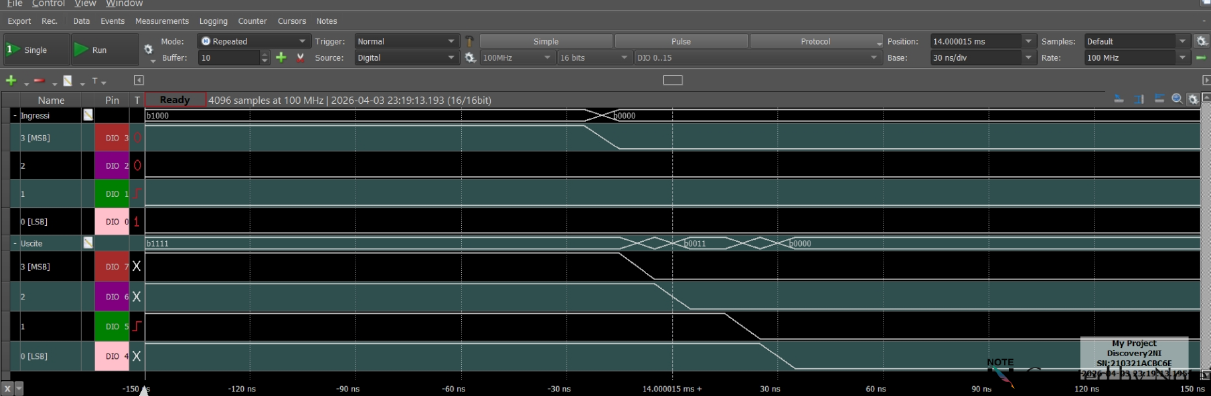
\includegraphics[width=1\linewidth]{1.png}
\end{center}

\noindent Osservando il transitorio (a cavallo di $t=14{,}000015\,\text{ms}$), è evidente come le singole linee in uscita dal blocco combinatorio scendano a zero in istanti sfalsati, generando temporaneamente un dato spuro (es. \texttt{b0011}). 
Grazie all'azione di campionamento del registro, tali irregolarità vengono confinate a monte: il circuito a valle viene aggiornato con precisione chirurgica e perfetta sincronia solo in corrispondenza del fronte di clock, garantendo un'uscita netta e priva di sfarfallii.

% ======================================================================
\chapter{Registri a scorrimento e contatori}
\textit{(17 aprile 2026)}

% ======================================================================
\section{Registri a scorrimento}

Un \textbf{registro a scorrimento} (shift register) è una catena di Flip-Flop di tipo D collegati in serie: l'uscita $Q$ di ciascuno è collegata all'ingresso $D$ del successivo. Ad ogni fronte di clock, ogni Flip-Flop «passa» il proprio valore al vicino di destra, come in un nastro trasportatore. In questo modo il dato si \emph{sposta} di una posizione ad ogni colpo di clock.

\vspace{2mm}
\noindent Per chiarire con un esempio: se il registro contiene i bit $[X, Y, Z]$ e arriva un nuovo dato $W$ dall'ingresso, dopo un tick di clock il contenuto diventa $[W, X, Y]$: il vecchio $Z$ è uscito, $X$ e $Y$ sono slittati di una posizione, e il nuovo $W$ è entrato in testa.

\subsection{Modalità di trasmissione dati}

A seconda di come si alimentano i dati in ingresso e di come si leggono in uscita, lo stesso registro fisico può funzionare in quattro modalità distinte:

\begin{itemize}[leftmargin=1.5em]
    \item \textbf{SISO} (Serial In -- Serial Out): il dato entra un bit alla volta dall'ingresso seriale ed esce un bit alla volta dall'ultimo FF. Utilizzo principale: \textbf{ritardare} un segnale digitale di esattamente $n$ cicli di clock.
    \item \textbf{SIPO} (Serial In -- Parallel Out): il dato entra un bit alla volta, ma si leggono in uscita \emph{contemporaneamente} tutti i bit memorizzati. Utilizzo tipico: convertire una trasmissione seriale (es. linea RS-232) in un dato parallelo leggibile dalla CPU.
    \item \textbf{PISO} (Parallel In -- Serial Out): si caricano tutti i bit in un solo colpo (caricamento parallelo), poi li si trasmette uno alla volta. Utilizzo: serializzare un dato parallelo per inviarlo su un bus seriale.
    \item \textbf{PIPO} (Parallel In -- Parallel Out): caricamento parallelo e lettura parallela. Funziona come un \textbf{registro di memoria}: cattura uno snapshot di un dato a $n$ bit e lo mantiene in uscita fino al prossimo aggiornamento.
\end{itemize}

\subsection{Temporizzazione e vincoli}

Affinché il registro funzioni correttamente, il clock deve rispettare due vincoli temporali critici propri di ogni Flip-Flop:

\begin{important}
$T_P > T_H$, \quad $T_S + T_P < T_{CLK}$

\begin{itemize}[leftmargin=1.3em]
  \item $T_{setup}$ ($T_S$): il dato deve essere stabile sull'ingresso $D$ per almeno questo tempo \emph{prima} del fronte di clock, altrimenti non viene catturato correttamente.
  \item $T_{hold}$ ($T_H$): il dato deve rimanere stabile per almeno questo tempo \emph{dopo} il fronte di clock.
  \item $T_P$: tempo di propagazione attraverso il FF (quanto ci vuole affinché, dopo il fronte, l'uscita $Q$ si aggiorni e il nuovo valore sia pronto per il FF successivo).
  \item $I_N = D_{SR}$: dato seriale in ingresso al registro.
\end{itemize}
\end{important}

\noindent In parole semplici: il periodo del clock deve essere abbastanza lungo da permettere al segnale di attraversare il FF e di stabilizzarsi sul $D$ del successivo \emph{prima} che arrivi il fronte successivo. Se il clock è troppo veloce si leggono valori errati.

\medskip
\noindent Nei registri a scorrimento sono presenti i seguenti segnali di controllo:
\begin{itemize}[leftmargin=1.5em]
    \item \textbf{CLK}: sincronizza ogni scorrimento.
    \item \textbf{RESET/CLEAR}: azzera immediatamente l'intero registro.
    \item \textbf{SET}: forza l'uscita a $1$ (preset).
    \item \textbf{ENABLE}: quando basso, congela il registro bloccando gli scorrimenti.
\end{itemize}

\medskip
\noindent\textcolor{teal}{\textbf{Riassunto -- Differenza tra registro normale e registro a scorrimento:}}
\begin{itemize}[leftmargin=1.5em]
    \item \textbf{Registro normale (PIPO)}: cattura e conserva un dato multi-bit aggiornandolo in blocco. Non c'è scorrimento interno.
    \item \textbf{Registro a scorrimento}: conserva il dato \emph{e lo fa scorrere} di una posizione ad ogni clock, abilitando la conversione seriale$\leftrightarrow$parallelo e il ritardo digitale.
\end{itemize}

\subsection{Schemi dei registri (PIPO, SISO, SIPO, PISO)}

Di seguito sono riportati gli schemi a blocchi semplificati delle quattro configurazioni
(ogni blocco è un FF-D con ingresso $D$, uscita $Q$, ingresso di clock e ingressi asincroni
$S$ di set e $R$ di reset). Nel PISO un multiplexer sceglie, tramite il segnale
Shift/$\overline{\text{Load}}$, se il secondo flip-flop riceve il bit del flip-flop precedente
(shift, ingresso 1) oppure il dato parallelo $P_1$ (caricamento, ingresso 0).

\begin{figure}[H]
\centering
\begin{circuitikz}[scale=0.9, every node/.style={scale=0.9}, line width=0.8pt]
\tikzset{
  mypipo/.style={flipflop, flipflop def={t1=$D_0$, t6=$Q_0$, c2=1}},
  mypipo1/.style={flipflop, flipflop def={t1=$D_1$, t6=$Q_1$, c2=1}},
  mysiso0/.style={flipflop, flipflop def={t1=$D_0$, t6=$Q_0$, c2=1}},
  mysiso1/.style={flipflop, flipflop def={t1=$D_1$, t6=$Q_1$, c2=1}}
}

% ======== TOP ROW ========

% -------- PIPO --------
\begin{scope}[yshift=0cm]
\node[mypipo] (FF0) at (0,3.0) {};
\node[mypipo1] (FF1) at (0,0) {};

\draw (FF0.pin 1) ++(-1.0,0) -- (FF0.pin 1);
\draw (FF1.pin 1) ++(-1.0,0) -- (FF1.pin 1);
\draw (FF0.pin 6) -- ++(1.0,0);
\draw (FF1.pin 6) -- ++(1.0,0);

% CLK
\coordinate (clkstart) at (-2.5, -1.2);
\coordinate (cb1) at (-1.5, -1.2);
\draw (clkstart) node[left, font=\bfseries, text=blue!60!black] {CLK} -- (cb1);
\draw (cb1) -- (cb1 |- FF1.pin 2) -- (FF1.pin 2);
\draw (cb1 |- FF1.pin 2) node[circle,fill,inner sep=1.2pt]{} -- (cb1 |- FF0.pin 2) -- (FF0.pin 2);

\node[font=\Large\bfseries, text=black] at (0,-2.2) {PIPO};
\end{scope}

% -------- SISO --------
\begin{scope}[xshift=9cm]
\node[mysiso0] (FF0) at (0,1.25) {};
\node[mysiso1] (FF1) at (3.5,1.25) {};

\draw (FF0.pin 1) ++(-1.0,0) -- (FF0.pin 1);
\draw (FF1.pin 6) -- ++(1.0,0);

\draw (FF0.pin 6) -- ++(0.7,0) coordinate (q0_bot) -- (q0_bot |- FF1.pin 1) coordinate (q0_top) -- (FF1.pin 1);

\draw (FF0.north) -- (FF0.north |- 0,2.75) node[above, font=\small\bfseries] {S};
\draw (FF1.north) -- (FF1.north |- 0,2.75) node[above, font=\small\bfseries] {S};
\draw (FF0.south) -- (FF0.south |- 0,-0.2) node[below, font=\small\bfseries] {R};
\draw (FF1.south) -- (FF1.south |- 0,-0.2) node[below, font=\small\bfseries] {R};

% CLK
\coordinate (clkstart) at (-2.5, -1.0);
\coordinate (cb0) at (-1.5, -1.0);
\coordinate (cb1) at (2.0, -1.0);
\draw (clkstart) node[left, font=\bfseries, text=blue!60!black] {CLK} -- (cb1);
\draw (cb0) -- (cb0 |- FF0.pin 2) -- (FF0.pin 2);
\draw (cb1) -- (cb1 |- FF1.pin 2) -- (FF1.pin 2);

\node[font=\Large\bfseries, text=black] at (1.75,-2.2) {SISO};
\end{scope}

% ======== BOTTOM ROW ========

% -------- SIPO --------
\begin{scope}[yshift=-8cm]
\node[mysiso0] (FF0) at (0,1.25) {};
\node[mysiso1] (FF1) at (3.5,1.25) {};

\draw (FF0.pin 1) ++(-1.0,0) -- (FF0.pin 1);
\draw (FF0.pin 6) -- ++(0.7,0) coordinate (q0_bot) -- (q0_bot |- FF1.pin 1) coordinate (q0_top) -- (FF1.pin 1);
\draw (FF1.pin 6) -- ++(0.7,0) coordinate (q1_bot);

\draw (FF0.north) -- (FF0.north |- 0,2.75) node[above, font=\small\bfseries] {S};
\draw (FF1.north) -- (FF1.north |- 0,2.75) node[above, font=\small\bfseries] {S};
\draw (FF0.south) -- (FF0.south |- 0,-0.2) node[below, font=\small\bfseries] {R};
\draw (FF1.south) -- (FF1.south |- 0,-0.2) node[below, font=\small\bfseries] {R};

% SIPO outputs
\draw (q0_top) node[circle, fill, inner sep=1.2pt] {} -- ++(0, 1.0);
\draw (q1_bot) node[circle, fill, inner sep=1.2pt] {} -- ++(0, 1.0);

% CLK
\coordinate (clkstart) at (-2.5, -1.0);
\coordinate (cb0) at (-1.5, -1.0);
\coordinate (cb1) at (2.0, -1.0);
\draw (clkstart) node[left, font=\bfseries, text=blue!60!black] {CLK} -- (cb1);
\draw (cb0) -- (cb0 |- FF0.pin 2) -- (FF0.pin 2);
\draw (cb1) -- (cb1 |- FF1.pin 2) -- (FF1.pin 2);

\node[font=\Large\bfseries, text=black] at (1.75,-2.2) {SIPO};
\end{scope}

% -------- PISO --------
\begin{scope}[xshift=9cm, yshift=-8cm]
\node[mysiso0] (FF0) at (0,1.25) {};
\node[mysiso1] (FF1) at (4.6,1.25) {};

\draw (FF0.north) -- (FF0.north |- 0,2.85) node[above, font=\small\bfseries] {S};
\draw (FF1.north) -- (FF1.north |- 0,2.85) node[above, font=\small\bfseries] {S};
\draw (FF0.south) -- (FF0.south |- 0,-0.3) node[below, font=\small\bfseries] {R};
\draw (FF1.south) -- (FF1.south |- 0,-0.3) node[below, font=\small\bfseries] {R};

% MUX block
\path (FF1.pin 1) ++(-0.6,0) node[draw, fill=gray!20, minimum height=0.9cm, minimum width=0.6cm, anchor=east] (mux) {\scriptsize MUX};

% Ingresso parallelo P0
\draw (FF0.pin 1 |- 0,2.85) ++(-0.6,0) coordinate (p0_start) node[above, font=\small\bfseries] {$P_0$};
\draw[->] (p0_start) |- (FF0.pin 1);

% Ingresso seriale Q0 -> ingresso 0 del MUX
\draw (FF0.pin 6) -- ++(0.5,0) |- ([yshift=-8pt]mux.west) node[left, font=\tiny] {1};

% Ingresso parallelo P1 -> ingresso 1 del MUX
\draw ([yshift=8pt]mux.west |- 0,2.85) ++(-0.4,0) coordinate (p1_start) node[above, font=\small\bfseries] {$P_1$};
\draw[->] (p1_start) |- ([yshift=8pt]mux.west) node[left, font=\tiny] {0};

\draw (mux.east) -- (FF1.pin 1);
\draw (FF1.pin 6) -- ++(1.0,0);

% Linea di selezione dal basso
\draw[<-, thick, gray!70!black] (mux.south) -- ++(0,-0.6) node[below, font=\scriptsize\bfseries, text=gray!80!black] {Shift/$\overline{\text{Load}}$};

% CLK
\coordinate (clkstart) at (-2.5, -1.0);
\coordinate (cb0) at (-1.5, -1.0);
\coordinate (cb1) at (2.6, -1.0);
\draw (clkstart) node[left, font=\bfseries, text=blue!60!black] {CLK} -- (cb1);
\draw (cb0) -- (cb0 |- FF0.pin 2) -- (FF0.pin 2);
\draw (cb1) -- (cb1 |- FF1.pin 2) -- (FF1.pin 2);

\node[font=\Large\bfseries, text=black] at (2.3,-2.2) {PISO};
\end{scope}

\end{circuitikz}
\caption{Schemi a blocchi dei registri a scorrimento: PIPO, SISO, SIPO, e PISO.}
\end{figure}

% ======================================================================
\section{Contatori}
\textit{(17 aprile 2026)}

\begin{definizione}{Contatore}
circuito sequenziale che avanza automaticamente di stato ad ogni fronte di clock, rappresentando in uscita la sequenza binaria $0, 1, 2, 3, \ldots$ (o la sua inversa, nei contatori \emph{down}).
\end{definizione}

\noindent L'idea alla base è semplice: ogni bit dell'uscita binaria cambia a frequenza dimezzata rispetto al bit precedente.
\begin{itemize}[leftmargin=1.5em]
    \item $Q_0$ (bit meno significativo) commuta ad \textbf{ogni} periodo di clock: è il più veloce.
    \item $Q_1$ commuta ogni \textbf{2} periodi: lo fa quando $Q_0$ scende da $1$ a $0$ (fronte di discesa).
    \item $Q_{i+1}$ commuta ogni $2^{i+1}$ periodi: in generale ogni bit commuta quando il bit precedente ha un fronte di discesa.
\end{itemize}
\noindent Questo comportamento rende i contatori anche utili come \textbf{divisori di frequenza}: il clock ha frequenza $f$; $Q_0$ oscilla a $f/2$; $Q_1$ a $f/4$; e così via.

\begin{center}
\begin{tikzpicture}[scale=0.9, every node/.style={scale=0.9}]
% Asse del tempo in basso
\draw[-latex, thick] (-0.8,-0.5) -- (9.0,-0.5) node[right, font=\small] {$t$};

% Linee verticali tratteggiate di guida
\foreach \x in {1.0, 2.0, 3.0, 4.0, 5.0, 6.0, 7.0, 8.0}{
    \draw[dashed, gray!35] (\x, -0.5) -- (\x, 3.0);
}

% CLK
\node[left, font=\small\bfseries] at (-0.8, 2.4) {CLK};
\draw[thick] (0,2.1)
\foreach \x in {0,1,2,3,4,5,6,7}{
  -- ++(0.5,0) -- ++(0,0.6) -- ++(0.5,0) -- ++(0,-0.6)
} -- ++(0.5,0);

% Q0 (f/2)
\node[left, font=\small\bfseries, color=blue!80!black] at (-0.8, 1.4) {$Q_0$ ($f/2$)};
\draw[thick, blue!80!black] (0,1.1)
\foreach \x in {0,2,4,6}{
  -- ++(1.0,0) -- ++(0,0.6) -- ++(1.0,0) -- ++(0,-0.6)
} -- ++(0.5,0);

% Q1 (f/4)
\node[left, font=\small\bfseries, color=red!80!black] at (-0.8, 0.4) {$Q_1$ ($f/4$)};
\draw[thick, red!80!black] (0,0.1)
\foreach \x in {0,4}{
  -- ++(2.0,0) -- ++(0,0.6) -- ++(2.0,0) -- ++(0,-0.6)
} -- ++(0.5,0);

\end{tikzpicture}
\end{center}

\subsection{Contatore asincrono (ripple counter)}

Nel contatore asincrono, il clock \textbf{non arriva a tutti i Flip-Flop contemporaneamente}. Solo il primo FF riceve il clock esterno; ogni FF successivo usa come proprio clock l'uscita $Q$ del FF precedente. I flip-flop sono sensibili al fronte di discesa (pallino sull'ingresso di clock) e hanno $J=K=1$ (modalità toggle): ogni FF commuta quando l'uscita del precedente passa da 1 a 0, realizzando un conteggio in avanti.

\medskip
\noindent\textcolor{teal}{\textbf{Il problema: la propagazione a catena (ripple).}} Poiché ogni FF deve aspettare che quello precedente abbia commutato, il segnale si propaga a cascata (da qui il nome \emph{ripple}). Il bit più significativo $Q_{n-1}$ non è aggiornato finché il segnale non ha attraversato tutti gli $n$ FF. Il ritardo totale vale:
\[
T_n = n \cdot T_P
\]
Questo impone che il periodo del clock sia sufficientemente lungo da permettere a tutta la catena di assestarsi prima del fronte successivo:
\[
T_{CLK} > n \cdot T_P
\]
Nei circuiti ad alta velocità questo è un limite importante: aggiungere Flip-Flop obbliga a rallentare il clock.

\begin{fitcenter}
\begin{circuitikz}[scale=0.88, every node/.style={scale=0.88}, line width=0.8pt]
\tikzset{
  jkbox/.style={
    draw, thick, minimum width=1.3cm, minimum height=1.8cm, inner sep=0pt
  }
}

% 4 Flip-Flop
\foreach \i/\x in {0/0, 1/3.2, 2/6.4, 3/9.6}{
  \node[jkbox] (B\i) at (\x, 0) {};
  % Ingressi J (in alto) e K (sotto)
  \node[font=\small\bfseries, right=2pt] at ([yshift=0.45cm]B\i.west) {$J_{\i}$};
  \node[font=\small\bfseries, right=2pt] at ([yshift=-0.05cm]B\i.west) {$K_{\i}$};
  
  % Clock negato in basso a sinistra (bubble + triangle)
  \draw ([yshift=-0.55cm]B\i.west) ++(-0.14, 0) circle (0.07cm);
  \draw ([yshift=-0.55cm]B\i.west) ++(0, 0.11) -- ++(0.16, -0.11) -- ++(-0.16, -0.11);
  \coordinate (clkpin\i) at ([yshift=-0.55cm]B\i.west);
  \coordinate (clkext\i) at ([xshift=-0.21cm, yshift=-0.55cm]B\i.west);

  % Uscita Q a destra, allineata al clock
  \node[font=\small\bfseries, left=2pt] at ([yshift=-0.55cm]B\i.east) {$Q_{\i}$};
  \coordinate (qpin\i) at ([yshift=-0.55cm]B\i.east);

  % J e K uniti insieme e salita alla barra 1
  \draw ([yshift=0.45cm]B\i.west) -- ++(-0.3, 0) coordinate (jterm\i)
     -- ([yshift=-0.05cm]B\i.west -| jterm\i) -- ([yshift=-0.05cm]B\i.west);
     
  \coordinate (midjk\i) at ($(jterm\i)!0.5!([yshift=-0.05cm]B\i.west -| jterm\i)$);
  \draw (midjk\i) -- (midjk\i |- 0, 1.45) coordinate (topconn\i);
}

% Barra orizzontale 1 in alto
\draw[thick] (-1.4, 1.45) node[left=3pt, font=\large\bfseries] {1} -- (topconn3);
\foreach \i in {0,1,2}{
  \fill (topconn\i) circle (1.5pt);
}

% Clock esterno
\draw[thick] (-0.9, -0.55) node[left, font=\small\bfseries] {CLK} -- (clkext0);

% Collegamenti a cascata: Q0 -> CLK1, Q1 -> CLK2, Q2 -> CLK3
\draw[thick] (qpin0) -- (clkext1);
\draw[thick] (qpin1) -- (clkext2);
\draw[thick] (qpin2) -- (clkext3);
\draw[-latex, thick] (qpin3) -- ++(0.7, 0);

\node[font=\small\bfseries, color=noteblue] at (4.8, -1.4) {CONTATORE ASINCRONO (RIPPLE COUNTER)};
\end{circuitikz}
\end{fitcenter}

\subsection{Contatore sincrono}

Nel contatore sincrono, il clock \textbf{arriva contemporaneamente a tutti i Flip-Flop}, eliminando il ritardo a cascata e rendendo il contatore molto più veloce.

\medskip
\noindent\textbf{Come si implementa la logica di conteggio?} Non tutti i FF devono commutare ad ogni tick: $Q_1$ deve commutare solo quando $Q_0=1$; $Q_2$ solo quando $Q_0=Q_1=1$; e così via. Questa condizione viene realizzata con \textbf{porte AND in cascata}: l'ingresso $J,K$ del FF $i$-esimo è connesso all'uscita di una porta AND che combina tutti i bit $Q_0, \ldots, Q_{i-1}$. Il FF $i$ riceve il permesso di commutare solo quando tutti i bit meno significativi valgono $1$.

\begin{fitcenter}
\begin{circuitikz}[scale=0.88, every node/.style={scale=0.88}, line width=0.8pt]
\tikzset{
  jkbox/.style={
    draw, thick, minimum width=1.3cm, minimum height=1.8cm, inner sep=0pt
  }
}

% 4 Flip-Flop
\foreach \i/\x in {0/0, 1/3.4, 2/7.0, 3/10.6}{
  \node[jkbox] (B\i) at (\x, 0) {};
  % Ingressi K (in alto) e J (sotto)
  \node[font=\small\bfseries, right=2pt] at ([yshift=0.45cm]B\i.west) {$K_{\i}$};
  \node[font=\small\bfseries, right=2pt] at ([yshift=-0.05cm]B\i.west) {$J_{\i}$};
  
  % Clock negato in basso a sinistra (bubble + triangle)
  \draw ([yshift=-0.55cm]B\i.west) ++(-0.14, 0) circle (0.07cm);
  \draw ([yshift=-0.55cm]B\i.west) ++(0, 0.11) -- ++(0.16, -0.11) -- ++(-0.16, -0.11);
  \coordinate (clkpin\i) at ([yshift=-0.55cm]B\i.west);
  \coordinate (clkext\i) at ([xshift=-0.21cm, yshift=-0.55cm]B\i.west);
  \coordinate (clktap\i) at ([xshift=-0.40cm, yshift=-0.55cm]B\i.west);

  % Uscita Q a destra
  \node[font=\small\bfseries, left=2pt] at ([yshift=-0.55cm]B\i.east) {$Q_{\i}$};
  \coordinate (qpin\i) at ([yshift=-0.55cm]B\i.east);

  % K e J uniti
  \coordinate (kterm\i) at ([xshift=-0.35cm, yshift=0.45cm]B\i.west);
  \coordinate (jterm\i) at ([xshift=-0.35cm, yshift=-0.05cm]B\i.west);
  \draw ([yshift=0.45cm]B\i.west) -- (kterm\i);
  \draw ([yshift=-0.05cm]B\i.west) -- (jterm\i);
}

% FF0: K0 e J0 collegati al livello logico 1
\draw[thick] (kterm0) -- (jterm0);
\draw[thick] ($(kterm0)!0.5!(jterm0)$) -- ++(-0.35, 0) -- ++(0, 0.8) node[above, font=\large\bfseries] {1};

% FF1: Q0 va al tratto verticale di K1-J1 che sale sopra FF1 verso AND1
\coordinate (vert1) at (kterm1);
\draw[thick] (qpin0) -- (qpin0 -| vert1) -- (jterm1) node[circle, fill, inner sep=1.1pt]{} -- (kterm1) node[circle, fill, inner sep=1.1pt]{} -- ([yshift=0.9cm]kterm1) coordinate (topFF1);

% AND1 tra FF1 e FF2
\node[and port, scale=0.65] (AND1) at (5.3, 0.45) {};
\draw[thick] (topFF1) -- (topFF1 -| AND1.in 1) -- (AND1.in 1);
\draw[thick] (qpin1) -- (qpin1 -| AND1.in 2) -- (AND1.in 2);

% Uscita AND1 va al tratto verticale di K2-J2 che sale sopra FF2 verso AND2
\coordinate (vert2) at (kterm2);
\draw[thick] (AND1.out) -- (vert2) node[circle, fill, inner sep=1.2pt]{} -- (jterm2);
\draw[thick] (vert2) -- ([yshift=0.9cm]kterm2) coordinate (topFF2);

% AND2 tra FF2 e FF3
\node[and port, scale=0.65] (AND2) at (8.9, 0.45) {};
\draw[thick] (topFF2) -- (topFF2 -| AND2.in 1) -- (AND2.in 1);
\draw[thick] (qpin2) -- (qpin2 -| AND2.in 2) -- (AND2.in 2);

% Uscita AND2 va a K3-J3 di FF3
\coordinate (vert3) at (kterm3);
\draw[thick] (AND2.out) -- (vert3) node[circle, fill, inner sep=1.2pt]{} -- (jterm3);

% Uscita Q3 finale
\draw[-latex, thick] (qpin3) -- ++(0.7, 0);

% Bus CLK comune in basso
\coordinate (clkbus_y) at (0, -1.2);
\draw[thick] (-1.6, -1.2) node[left=2pt, font=\small\bfseries] {CLK} -- (11.4, -1.2);
\foreach \i in {0,1,2,3}{
  \draw[thick] (clkext\i) -- (clktap\i) |- (clktap\i |- clkbus_y) node[circle, fill, inner sep=1.2pt]{};
}

\node[font=\small\bfseries, color=noteblue] at (5.3, -1.7) {CONTATORE SINCRONO};
\end{circuitikz}
\end{fitcenter}

\subsection{Azzeramento dopo un certo conteggio (contatore modulo-M)}

Spesso non si vuole un contatore che vada da $0$ a $2^n-1$, ma che si fermi ad un numero specifico $M$ e poi riparta da zero.

\medskip
\noindent\textbf{Implementazione:} si aggiunge una porta AND ai cui ingressi arrivano le uscite $Q_i$ che sono a $1$ nella rappresentazione binaria di $M$. Non appena il contatore raggiunge $M$, l'uscita della porta AND va a $1$ e genera un segnale di \textbf{RESET asincrono} che azzera immediatamente tutti i FF riportandoli a $Q=0000$.

\medskip
\noindent\textbf{Attenzione al glitch sull'ultimo conteggio:} il valore $M$ compare realmente in uscita per un brevissimo istante (il tempo necessario affinché la porta AND lo riconosca e il reset arrivi) prima che tutto sia azzerato. L'ultimo stato ha quindi una durata anomala:
\[
T_{\text{stato }M} = T_f(\text{JK-FF}) + T_P(\text{AND})
\]

\medskip
\begin{esercizio}{Esempio: azzeramento dopo il numero 5 (bastano 3 bit)}
Quando $Q_3 Q_2 Q_1 Q_0 = 0101_2$ (valore 5), la porta AND sottostante rileva questa condizione (alimentata da $Q_0$ e $Q_2$, gli unici bit a 1 di $5=101_2$) e genera il segnale di \textbf{RESET asincrono di tutti i FF}, che vengono azzerati attraverso i loro ingressi di clear.\\[0.3em]
Il contatore percorre quindi gli stati $0, 1, 2, 3, 4$, ciascuno per un periodo di clock, mentre lo stato 5 compare solo per il brevissimo tempo $T_f(\text{JK-FF}) + T_P(\text{AND})$ necessario all'azzeramento. Il ciclo dura 5 periodi di clock: si tratta di un \textbf{contatore modulo-5} (divisore per 5). Per ottenere un modulo-$M$ con reset asincrono si decodifica quindi il valore $M$ stesso.
\end{esercizio}

\begin{fitcenter}
\begin{circuitikz}[scale=0.88, every node/.style={scale=0.88}, line width=0.8pt]
\tikzset{
  jkbox/.style={
    draw, thick, minimum width=1.3cm, minimum height=1.8cm, inner sep=0pt
  }
}

% 4 Flip-Flop
\foreach \i/\x in {0/0, 1/3.4, 2/7.0, 3/10.6}{
  \node[jkbox] (B\i) at (\x, 0) {};
  \node[font=\small\bfseries, right=2pt] at ([yshift=0.45cm]B\i.west) {$K_{\i}$};
  \node[font=\small\bfseries, right=2pt] at ([yshift=-0.05cm]B\i.west) {$J_{\i}$};
  
  % Clock negato in basso a sinistra
  \draw ([yshift=-0.55cm]B\i.west) ++(-0.14, 0) circle (0.07cm);
  \draw ([yshift=-0.55cm]B\i.west) ++(0, 0.11) -- ++(0.16, -0.11) -- ++(-0.16, -0.11);
  \coordinate (clkpin\i) at ([yshift=-0.55cm]B\i.west);
  \coordinate (clkext\i) at ([xshift=-0.21cm, yshift=-0.55cm]B\i.west);
  \coordinate (clktap\i) at ([xshift=-0.40cm, yshift=-0.55cm]B\i.west);

  % Uscita Q a destra
  \node[font=\small\bfseries, left=2pt] at ([yshift=-0.55cm]B\i.east) {$Q_{\i}$};
  \coordinate (qpin\i) at ([yshift=-0.55cm]B\i.east);

  % K e J uniti
  \coordinate (kterm\i) at ([xshift=-0.35cm, yshift=0.45cm]B\i.west);
  \coordinate (jterm\i) at ([xshift=-0.35cm, yshift=-0.05cm]B\i.west);
  \draw ([yshift=0.45cm]B\i.west) -- (kterm\i);
  \draw ([yshift=-0.05cm]B\i.west) -- (jterm\i);
}

% FF0: K0 e J0 collegati a 1
\draw[thick] (kterm0) -- (jterm0);
\draw[thick] ($(kterm0)!0.5!(jterm0)$) -- ++(-0.35, 0) -- ++(0, 0.8) node[above, font=\large\bfseries] {1};

% FF1: Q0 va al tratto verticale di K1-J1 che sale sopra FF1 verso AND1
\coordinate (vert1) at (kterm1);
\draw[thick] (qpin0) -- (qpin0 -| vert1) -- (jterm1) node[circle, fill, inner sep=1.1pt]{} -- (kterm1) node[circle, fill, inner sep=1.1pt]{} -- ([yshift=0.9cm]kterm1) coordinate (topFF1);

% AND1 tra FF1 e FF2
\node[and port, scale=0.65] (AND1) at (5.3, 0.45) {};
\draw[thick] (topFF1) -- (topFF1 -| AND1.in 1) -- (AND1.in 1);
\draw[thick] (qpin1) -- (qpin1 -| AND1.in 2) -- (AND1.in 2);

% Uscita AND1 va al tratto verticale di K2-J2 che sale sopra FF2 verso AND2
\coordinate (vert2) at (kterm2);
\draw[thick] (AND1.out) -- (vert2) node[circle, fill, inner sep=1.2pt]{} -- (jterm2);
\draw[thick] (vert2) -- ([yshift=0.9cm]kterm2) coordinate (topFF2);

% AND2 tra FF2 e FF3
\node[and port, scale=0.65] (AND2) at (8.9, 0.45) {};
\draw[thick] (topFF2) -- (topFF2 -| AND2.in 1) -- (AND2.in 1);
\draw[thick] (qpin2) -- (qpin2 -| AND2.in 2) -- (AND2.in 2);

% Uscita AND2 va a K3-J3 di FF3
\coordinate (vert3) at (kterm3);
\draw[thick] (AND2.out) -- (vert3) node[circle, fill, inner sep=1.2pt]{} -- (jterm3);

% Uscita Q3 finale
\draw[-latex, thick] (qpin3) -- ++(0.7, 0);

% Bus CLK comune in basso
\coordinate (clkbus_y) at (0, -1.2);
\draw[thick] (-1.6, -1.2) node[left=2pt, font=\small\bfseries] {CLK} -- (11.4, -1.2);
\foreach \i in {0,1,2,3}{
  \draw[thick] (clkext\i) -- (clktap\i) |- (clktap\i |- clkbus_y) node[circle, fill, inner sep=1.2pt]{};
}

% Logica di RESET ASINCRONO: in 1 ancorato esattamente sotto Q2
\node[and port, scale=0.75, anchor=in 1] (AND_RST) at (qpin2 |- 0, -2.0) {};

% Linea da Q0 verso l'AND di reset (in basso)
\fill[gray!60!black] (1.6, -0.55) circle (1.3pt);
\draw[thick, gray!60!black] (1.6, -0.55) |- (AND_RST.in 2);

% Linea da Q2 verso l'AND di reset (scende diritta da Q2 direttamente nell'ingresso 1)
\fill[gray!60!black] (qpin2) circle (1.3pt);
\draw[thick, gray!60!black] (qpin2) -- (AND_RST.in 1);

% Uscita Reset sotto FF3
\draw[thick, gray!60!black] (AND_RST.out) -- ++(0.3, 0) node[right, font=\footnotesize\bfseries, text=gray!60!black] {RESET ASINCRONO DI TUTTI I FF};

\end{circuitikz}
\end{fitcenter}

\clearpage
\subsection{Ripple Carry Output (RCO)}

I contatori binari integrati (come il classico \textbf{SN74LS163A}) includono un'uscita speciale chiamata \textbf{RCO} (Ripple Carry Output).

\medskip
\noindent\textbf{A cosa serve?} Quando si collegano più chip in cascata per formare un contatore a più bit (es. 8, 12, 16 bit), ogni chip deve segnalare al successivo quando ha terminato il proprio ciclo di conteggio. Il chip delle unità segnala al chip delle decine; il chip delle decine segnala a quello delle centinaia; e così via.

L'RCO è l'uscita di una porta NOR con 5 ingressi (i 4 $\overline{Q_i}$ e il segnale di \emph{enable} $T$ negato, cioè $\text{RCO}=T\cdot Q_AQ_BQ_CQ_D$): va a $1$ per esattamente \textbf{un periodo di clock} quando il contatore ha raggiunto il valore massimo (tipicamente $Q=1111=15$). Solo in quel preciso istante tutti i $\overline{Q_i}$ sono a $0$, e la NOR dà $1$:
\[
\text{RCO} = 1 \quad \text{per un periodo } T_{CLK} \text{ quando il conteggio è al massimo.}
\]

\noindent Il chip successivo nella catena usa questo impulso RCO come \emph{enable} (o come clock) per incrementare il proprio conteggio: in questo modo si realizzano contatori a 8, 12, 16 bit collegando semplicemente chip da 4 bit in cascata tramite RCO.

\begin{center}
\begin{tikzpicture}[scale=0.75, every node/.style={scale=0.75}]
% Corpo integrato
\draw[thick, fill=blue!3] (0,0) rectangle (5.0, 5.8);
\node[font=\large\bfseries, color=noteblue] at (2.5, 5.25) {SN74LS163A};
\node[font=\scriptsize, color=gray] at (2.5, 4.85) {Contatore sincrono a 4 bit};

% Ingressi di controllo (sinistra alto)
\foreach \y/\lab in {4.3/CLK, 3.7/$\overline{\text{CLR}}$, 3.1/$\overline{\text{LOAD}}$, 2.5/ENP, 1.9/ENT}{
  \draw[-latex, thick] (-1.2, \y) node[left, font=\small\bfseries]{\lab} -- (0, \y);
}

% Ingressi dati paralleli (sinistra basso)
\foreach \y/\lab in {1.3/A, 0.95/B, 0.6/C, 0.25/D}{
  \draw[-latex] (-1.2, \y) node[left, font=\footnotesize]{DATA \lab} -- (0, \y);
}

% Uscite dati (destra)
\foreach \y/\lab in {4.3/$Q_A$, 3.5/$Q_B$, 2.7/$Q_C$, 1.9/$Q_D$}{
  \draw[-latex, thick] (5.0, \y) -- (6.2, \y) node[right, font=\small\bfseries]{\lab};
}

% Uscita RCO (destra basso)
\draw[-latex, thick, color=noteblue] (5.0, 0.9) -- (6.2, 0.9) node[right, font=\small\bfseries]{RCO};
\node[left, font=\scriptsize, color=gray] at (5.0, 0.9) {Carry};

\end{tikzpicture}
\end{center}

% ======================================================================
\chapter{Conteggio, divisori di frequenza e PRFG}
\textit{(20 aprile 2026)}

% Simbolo del contatore SN74LS163 usato nelle figure del capitolo.
% Coordinate dei pin: (<nome pic>-P), -T, -CLK, -D, -C, -B, -A, -LOAD, -CLR,
% -RCO, -QD, -QC, -QB, -QA (estremità esterna del terminale).
\tikzset{
  chip163/.pic={
    \draw[thick, fill=noteblue!4] (0,0) rectangle (2.4,5.2);
    \node[font=\small\bfseries] at (1.2,5.5) {74LS163};
    \foreach \nm/\y/\num in {P/4.8/7, T/4.3/10, D/3.1/6, C/2.6/5, B/2.1/4, A/1.6/3}{
      \draw (0,\y) -- (-0.5,\y) coordinate (-\nm);
      \node[font=\scriptsize, anchor=west] at (0.06,\y) {\nm};
      \node[font=\tiny, above, inner sep=1pt] at (-0.25,\y) {\num};
    }
    \draw (0,3.7) -- (-0.5,3.7) coordinate (-CLK);
    \draw (0,3.55) -- (0.16,3.7) -- (0,3.85);
    \node[font=\scriptsize, anchor=west] at (0.2,3.7) {CLK};
    \node[font=\tiny, above, inner sep=1pt] at (-0.25,3.7) {2};
    \foreach \nm/\y/\num in {LOAD/1.0/9, CLR/0.4/1}{
      \draw (-0.07,\y) circle (0.07);
      \draw (-0.14,\y) -- (-0.5,\y) coordinate (-\nm);
      \node[font=\scriptsize, anchor=west] at (0.06,\y) {\nm};
      \node[font=\tiny, above, inner sep=1pt] at (-0.32,\y) {\num};
    }
    \foreach \nm/\lab/\y/\num in {RCO/RCO/4.3/15, QD/$Q_D$/3.1/11, QC/$Q_C$/2.6/12, QB/$Q_B$/2.1/13, QA/$Q_A$/1.6/14}{
      \draw (2.4,\y) -- (2.9,\y) coordinate (-\nm);
      \node[font=\scriptsize, anchor=east] at (2.34,\y) {\lab};
      \node[font=\tiny, above, inner sep=1pt] at (2.65,\y) {\num};
    }
  },
  % generatore di clock (onda quadra) con uscita sul lato destro
  clockgen/.pic={
    \draw (-1.0,-0.3) rectangle (0,0.3);
    \draw[line width=0.5pt] (-0.86,-0.15) -- ++(0,0.3) -- ++(0.18,0) -- ++(0,-0.3)
      -- ++(0.18,0) -- ++(0,0.3) -- ++(0.18,0) -- ++(0,-0.3) -- ++(0.18,0) -- ++(0,0.3);
    \coordinate (-out) at (0,0);
  }
}

\noindent In questo capitolo i contatori e i registri a scorrimento visti nel capitolo
precedente vengono usati come ``mattoni'' per costruire tre famiglie di circuiti:
contatori a più bit ottenuti collegando più integrati in \textbf{cascata}, \textbf{divisori
di frequenza} per un numero intero $n$ e \textbf{generatori di sequenze pseudo casuali}.

% ======================================================================
\section{Contatori a 8 bit: cascata di due SN74LS163}

\subsection{Richiamo: i terminali del SN74LS163}

Il SN74LS163 è un contatore binario \textbf{sincrono} a 4 bit: tutte le sue operazioni
(conteggio, caricamento, azzeramento) avvengono sul fronte di salita del clock.

\begin{center}
\small
\begin{tabular}{c l p{0.62\linewidth}}
\toprule
Pin & Nome & Funzione \\
\midrule
2 & CLK & clock: il contatore cambia stato solo sul fronte di salita \\
7, 10 & P, T & abilitazioni del conteggio (ENP, ENT): il contatore avanza solo se $P=T=1$ \\
3, 4, 5, 6 & $A$, $B$, $C$, $D$ & ingressi paralleli per il caricamento ($A$ = LSB) \\
9 & $\overline{\text{LOAD}}$ & caricamento \textbf{sincrono}, attivo basso: se vale 0, al fronte successivo $Q_DQ_CQ_BQ_A = DCBA$ \\
1 & $\overline{\text{CLR}}$ & azzeramento \textbf{sincrono}, attivo basso: se vale 0, al fronte successivo $Q_DQ_CQ_BQ_A = 0000$ \\
14, 13, 12, 11 & $Q_A \ldots Q_D$ & uscite del conteggio ($Q_A$ = LSB) \\
15 & RCO & \emph{Ripple Carry Output}: $\text{RCO} = T\cdot Q_A Q_B Q_C Q_D$, vale 1 solo nello stato 1111 \\
\bottomrule
\end{tabular}
\end{center}

\noindent Gli ingressi di controllo hanno una precisa \textbf{priorità}:
$\overline{\text{CLR}}$ prevale su $\overline{\text{LOAD}}$, che a sua volta prevale sul
conteggio; se $P\cdot T=0$ (e gli altri comandi sono inattivi) il contatore mantiene lo
stato (\emph{hold}). Nei simboli seguenti il pallino sui terminali LOAD e CLR indica che
sono attivi bassi.

\subsection{Collegamento in cascata}

Due contatori a 4 bit si collegano in \textbf{cascata} usando l'RCO del primo modulo come
\emph{enable di conteggio} del secondo:

\begin{fitcenter}
\begin{tikzpicture}[line width=0.6pt, font=\small, >=latex]
\pic (U1) at (0,0) {chip163};
\pic (U2) at (7.2,0) {chip163};
\node[font=\footnotesize, color=noteblue] at (1.2,-2.1) {modulo meno significativo (LSB)};
\node[font=\footnotesize, color=noteblue] at (8.4,-2.1) {modulo più significativo (MSB)};
% Enable comune agli ingressi P
\draw (-2.6,6.3) node[left, font=\scriptsize] {Enable} -- (6.2,6.3) |- (U2-P);
\draw (-1.9,6.3) node[circle, fill, inner sep=1.2pt] {} |- (U1-P);
% T del primo modulo e LOAD inattivi (livello logico 1)
\foreach \p in {U1-T, U1-LOAD, U2-LOAD}{
  \draw (\p) -- ++(-0.3,0) node[left, font=\scriptsize] {1};
}
% Riporto: RCO del primo -> T del secondo
\draw (U1-RCO) -- node[above, font=\scriptsize] {RCO$_1$} (U2-T);
% Clock comune
\pic (G) at (-2.6,3.7) {clockgen};
\node[above, font=\scriptsize] at (-3.1,4.0) {Count};
\draw (G-out) -- (U1-CLK);
\draw (-1.4,3.7) node[circle, fill, inner sep=1.2pt] {} -- (-1.4,0.55) arc[start angle=90, end angle=-90, radius=0.15] -- (-1.4,-0.8) -- (5.6,-0.8) |- (U2-CLK);
% Reset comune (CLR sincrono)
\draw (-2.6,-1.4) node[left, font=\scriptsize] {$\overline{\text{Reset}}$} -- (5.9,-1.4) |- (U2-CLR);
\draw (-1.9,-1.4) node[circle, fill, inner sep=1.2pt] {} |- (U1-CLR);
% Uscite
\foreach \q/\l in {QD/D, QC/C, QB/B, QA/A}{
  \draw[->] (U1-\q) -- ++(0.45,0) node[right, font=\scriptsize] {$\l$};
}
\foreach \q/\l in {QD/H, QC/G, QB/F, QA/E}{
  \draw[->] (U2-\q) -- ++(0.45,0) node[right, font=\scriptsize] {$\l$};
}
\draw[->] (U2-RCO) -- ++(0.45,0) node[right, font=\scriptsize] {RCO$_2$};
\end{tikzpicture}
\end{fitcenter}

\noindent Il funzionamento si ricava analizzando i collegamenti uno per uno:

\begin{itemize}[leftmargin=1.5em, itemsep=2pt]
    \item \textbf{Clock comune}: entrambi i moduli ricevono lo stesso segnale di clock
          (\emph{Count}). La cascata è quindi \textbf{sincrona}: tutti gli 8 bit commutano
          sullo stesso fronte, senza il ritardo a catena del contatore asincrono.
    \item \textbf{Enable}: collegato all'ingresso $P$ di entrambi i moduli, abilita o
          congela l'intero contatore a 8 bit. L'ingresso $T$ del primo modulo è fisso a 1.
    \item \textbf{Riporto}: l'ingresso $T$ del secondo modulo è pilotato da
          $\text{RCO}_1$, che vale 1 solo mentre il modulo LSB si trova nello stato
          $DCBA=1111$ (15). Il modulo MSB è quindi abilitato \emph{per un solo periodo di
          clock} ogni 16: al fronte successivo il modulo LSB passa da 15 a 0 e,
          contemporaneamente, il modulo MSB avanza di un'unità. È esattamente il riporto
          dell'addizione binaria.
    \item \textbf{$\overline{\text{LOAD}}$} è inattivo (a 1) e gli ingressi $DCBA$ non
          sono usati; \textbf{$\overline{\text{Reset}}$} è comune ai due $\overline{\text{CLR}}$:
          portandolo a 0 entrambi i moduli si azzerano al fronte di clock successivo
          (nel '163 il clear è sincrono).
\end{itemize}

\noindent Le uscite formano il numero a 8 bit $N = HGFE\,DCBA$, con $0 \le N \le 2^8-1=255$.
Il bit $E$ è il meno significativo dei quattro bit del modulo MSB e viene incrementato
ogni volta che il modulo LSB completa un ciclo. Ad esempio:
\[
N = 0000\,1111_2 = 15 \;\xrightarrow{\text{CLK}}\; N = 0001\,0000_2 = 16
\]
perché $DCBA$ passa da 1111 a 0000 e, essendo $\text{RCO}_1=1$, $HGFE$ passa da 0000 a 0001.
Ogni uscita divide la frequenza del clock per una potenza di 2: $f_A = f_{\text{CLK}}/2$,
$f_B = f_{\text{CLK}}/4$, \dots, fino a $f_H = f_{\text{CLK}}/256$.

\begin{osservazione}{Perché il riporto va su $T$ e non su $P$}
I due ingressi di abilitazione non sono equivalenti: $T$ entra anche nell'espressione
dell'RCO ($\text{RCO}=T\cdot Q_AQ_BQ_CQ_D$), $P$ no. Collegando il riporto a $T$,
$\text{RCO}_2$ vale 1 solo quando \emph{entrambi} i moduli sono a 15 (cioè $N=255$): il
riporto si propaga lungo la catena e un terzo modulo, collegato con $T_3=\text{RCO}_2$,
formerebbe un contatore a 12 bit. L'ingresso $P$ resta libero per l'abilitazione globale.
\end{osservazione}

% ======================================================================
\section{Divisori di frequenza per un numero $n$}

\begin{definizione}{Divisore di frequenza}
circuito sequenziale che riceve in ingresso il segnale di clock e ne riduce la frequenza di
un fattore intero $n$:
\[
f_{\text{out}} = \frac{f_{\text{CLK}}}{n} \qquad\qquad T_{\text{out}} = n\,T_{\text{CLK}}
\]
\end{definizione}

\noindent L'idea è semplice: un contatore che percorre ciclicamente $n$ stati ripete il
proprio comportamento ogni $n$ periodi di clock. Un segnale che vale 1 in uno solo degli
$n$ stati è quindi un treno di impulsi di durata $T_{\text{CLK}}$ e periodo
$n\,T_{\text{CLK}}$. Il contatore libero a 4 bit ha $2^4=16$ stati; per ottenere un
qualsiasi $n<16$ bisogna \textbf{accorciare il ciclo}. Con il SN74LS163 esistono due
tecniche, che sfruttano i due comandi sincroni:
\begin{itemize}[leftmargin=1.5em, itemsep=1pt]
    \item \textbf{CLEAR sincrono}: il contatore conta $0, 1, \ldots, n-1$ e poi si azzera;
    \item \textbf{LOAD sincrono}: il contatore riparte da un valore iniziale
          $N_{\text{load}}$ e conta fino a 15, percorrendo $16-N_{\text{load}}$ stati.
\end{itemize}

\subsection{Divisore con CLEAR sincrono}

Nel circuito seguente il contatore conta fino a $DCBA=1101$ (13); in quello stato il
comando di clear si attiva e al fronte successivo il conteggio ricomincia da 0.

\begin{fitcenter}
\begin{circuitikz}[line width=0.6pt, font=\small, >=latex]
\pic (U) at (0,0) {chip163};
% abilitazioni e LOAD inattivo
\foreach \p in {U-P, U-T, U-LOAD}{
  \draw (\p) -- ++(-0.3,0) node[left, font=\scriptsize] {1};
}
% ingressi dati non usati, collegati a 0
\draw (U-D) -- (U-D -| -0.9,0) -- (U-A -| -0.9,0) -- (U-A);
\foreach \p in {U-C, U-B}{
  \draw (\p) -- (\p -| -0.9,0) node[circle, fill, inner sep=1.1pt] {};
}
\draw (-0.9,2.35) -- (-1.25,2.35) node[left, font=\scriptsize] {0};
% clock
\pic (G) at (-1.9,3.7) {clockgen};
\draw (G-out) -- (U-CLK);
% decodifica dello stato 13 = 1101
\node[nand port, number inputs=4] (N) at (7.0,2.35) {};
\node[not port] (NB) at (4.0,2.1) {};
\draw (U-QB) -- (NB.in 1);
\draw (U-QD) -- (5.8,3.1) |- (N.in 1);
\draw (U-QC) -- (5.3,2.6) |- (N.in 2);
\draw (NB.out) -- (5.3,2.1) |- (N.in 3);
\draw (U-QA) -- (5.8,1.6) |- (N.in 4);
% uscita della NAND -> CLR
\draw (N.out) -- ++(0.4,0) coordinate (o);
\draw (o) -- (o |- 0,-0.9) -- (-1.6,-0.9) |- (U-CLR);
\node[circle, fill, inner sep=1.2pt] at (o) {};
\draw[->] (o) -- ++(0.9,0) node[right, font=\scriptsize, align=left] {uscita\\$f_{\text{CLK}}/14$};
\node[above, font=\scriptsize] at (3.6,-0.9) {$\overline{\text{CLR}}=\overline{Q_D\,Q_C\,\overline{Q_B}\,Q_A}$};
\end{circuitikz}
\end{fitcenter}

\noindent\textbf{Funzionamento.} La porta NAND a 4 ingressi riceve $Q_D$, $Q_C$,
$\overline{Q_B}$ (tramite l'invertitore) e $Q_A$: la sua uscita vale 0 \emph{solo} quando
$Q_DQ_CQ_BQ_A = 1101 = 13$. Poiché il clear del '163 è sincrono, in quello stato non
succede nulla di immediato: è il fronte di clock \emph{successivo} ad azzerare il contatore.
La sequenza è quindi
\[
0 \to 1 \to 2 \to \cdots \to 12 \to 13 \to 0 \to 1 \to \cdots
\]
cioè un ciclo di \textbf{14 stati}, ciascuno della durata di un periodo di clock:
\[
f_{\text{out}} = \frac{f_{\text{CLK}}}{14}
\]
Il segnale $\overline{\text{CLR}}$ stesso è un treno di impulsi bassi, larghi
$T_{\text{CLK}}$, con periodo $14\,T_{\text{CLK}}$. In generale, per dividere per $n$ con
il clear sincrono si decodifica lo stato $n-1$ (e non $n$), proprio perché l'azzeramento
avviene un colpo di clock dopo la decodifica.

\medskip
\noindent Osservazioni sulle singole uscite:
\begin{itemize}[leftmargin=1.5em, itemsep=2pt]
    \item $A$ (LSB) ha $T_A = 2\,T_{\text{CLK}}$: commuta a ogni colpo di clock e, poiché il
          ciclo ha un numero pari di stati, continua ad alternarsi regolarmente anche nel
          passaggio $13 \to 0$.
    \item $D$ (MSB) nel contatore libero ha $T_D = 16\,T_{\text{CLK}}$. Con il ciclo
          accorciato il suo periodo diventa $14\,T_{\text{CLK}}$, ma l'onda non è più
          simmetrica: $D=0$ negli stati $0$--$7$ (8 periodi) e $D=1$ negli stati $8$--$13$
          (6 periodi).
    \item Il numero 13 è l'ultimo contato e dura un periodo di clock intero.
\end{itemize}

\begin{important}
\textbf{Clear sincrono o asincrono?} Se il clear fosse \emph{asincrono} (come nel contatore
modulo-$M$ del capitolo precedente, o nel 74LS161), il contatore si azzererebbe non appena
raggiunto 13: l'ultimo stato durerebbe solo il tempo di propagazione della porta e del
contatore, cioè un \emph{glitch} e non un vero fronte di conteggio. Per dividere per 14
bisognerebbe allora decodificare 14, e l'impulso di azzeramento sarebbe brevissimo e poco
affidabile. Con il clear sincrono ogni stato, compreso l'ultimo, dura esattamente
$T_{\text{CLK}}$.
\end{important}

\subsection{Divisore con SET sincrono (LOAD)}

In questo secondo schema l'RCO, attraverso un invertitore, comanda l'ingresso
$\overline{\text{LOAD}}$: quando il contatore ha finito di contare viene caricato il
valore impostato sugli ingressi, $DCBA=0110$ (6).

\begin{fitcenter}
\begin{circuitikz}[line width=0.6pt, font=\small, >=latex]
\pic (U) at (0,0) {chip163};
% abilitazioni e CLR inattivo
\foreach \p in {U-P, U-T, U-CLR}{
  \draw (\p) -- ++(-0.3,0) node[left, font=\scriptsize] {1};
}
% valore di preset DCBA = 0110
\foreach \p/\v in {U-D/0, U-C/1, U-B/1, U-A/0}{
  \draw (\p) -- ++(-0.3,0) node[left, font=\scriptsize] {\v};
}
% clock
\pic (G) at (-1.9,3.7) {clockgen};
\draw (G-out) -- (U-CLK);
% RCO -> invertitore -> LOAD
\node[not port, xscale=-1] (NL) at (1.2,-0.9) {};
\draw (U-RCO) -- (4.0,4.3) coordinate (r) |- (NL.in 1);
\draw (NL.out) -| (-1.5,1.0) -- (U-LOAD);
\node[circle, fill, inner sep=1.2pt] at (r) {};
\draw[->] (r) -- ++(1.0,0) node[right, font=\scriptsize, align=left] {uscita RCO\\$f_{\text{CLK}}/10$};
\node[above, font=\scriptsize] at (-0.55,-0.9) {$\overline{\text{LOAD}}$};
% uscite
\foreach \q/\l in {QD/D, QC/C, QB/B, QA/A}{
  \draw[->] (U-\q) -- ++(0.45,0) node[right, font=\scriptsize] {$\l$};
}
\end{circuitikz}
\end{fitcenter}

\noindent\textbf{Funzionamento.} Durante il conteggio l'RCO vale 0 e quindi
$\overline{\text{LOAD}}=1$ (inattivo). Quando il contatore raggiunge 15 si ha
$\text{RCO}=1$, dunque $\overline{\text{LOAD}}=0$: al fronte successivo, invece di passare
a 0, il contatore carica il valore di preset $DCBA=0110=6$. La sequenza è
\[
6 \to 7 \to 8 \to \cdots \to 14 \to 15 \to 6 \to 7 \to \cdots
\]
e comprende $16-6=10$ stati. L'RCO vale 1 per un solo periodo di clock ogni 10, quindi
\[
f_{\text{RCO}} = \frac{f_{\text{CLK}}}{10}
\]
(un impulso per ciclo, largo $T_{\text{CLK}}$). In generale, con un contatore a $N$ bit e
un valore di caricamento $N_{\text{load}}$:
\[
T_{\text{out}} = \left(2^N - N_{\text{load}}\right) T_{\text{CLK}}
\qquad\Longrightarrow\qquad
N_{\text{load}} = 2^N - n
\]
Per dividere per $n=10$ con 4 bit si carica $16-10=6$; per $n=12$ si carica $4=0100$; per
$n=5$ si carica $11=1011$.

\begin{center}
\begin{tikzpicture}[x=0.62cm, y=0.5cm, font=\scriptsize, line width=0.6pt]
\node[left] at (-0.2,6.5) {CLK};
\draw (0,6) \foreach \k in {0,...,13}{ -- ++(0,1) -- ++(0.5,0) -- ++(0,-1) -- ++(0.5,0) };
\node[left] at (-0.2,4) {conteggio};
\foreach \v [count=\k from 0] in {13,14,15,6,7,8,9,10,11,12,13,14,15,6}{
  \draw (\k+0.12,3.5) -- (\k+0.88,3.5) -- (\k+1,4) -- (\k+0.88,4.5) -- (\k+0.12,4.5) -- (\k,4) -- cycle;
  \node at (\k+0.5,4) {\v};
}
\node[left] at (-0.2,1.5) {RCO};
\draw (0,1) -- (2,1) -- (2,2) -- (3,2) -- (3,1) -- (12,1) -- (12,2) -- (13,2) -- (13,1) -- (14,1);
\foreach \x in {2,3,12,13}{ \draw[dashed, gray] (\x,0.4) -- (\x,7.2); }
\draw[<->] (3,0.4) -- node[below] {$T_{\text{out}} = 10\,T_{\text{CLK}}$} (13,0.4);
\node[above, color=noteblue] at (3,4.6) {carica 6};
\node[above, color=noteblue] at (13,4.6) {carica 6};
\end{tikzpicture}
\end{center}

\noindent Rispetto al metodo del clear, il caricamento non richiede una porta di
decodifica a più ingressi (basta un invertitore sull'RCO) e il fattore di divisione si
cambia modificando soltanto i livelli sugli ingressi $DCBA$: con quattro interruttori si
ottiene un \textbf{divisore programmabile}.

\begin{important}
\textbf{Confronto fra i due metodi} (contatore a $N$ bit, divisione per $n$):
\begin{itemize}[leftmargin=1.3em, itemsep=2pt]
    \item \textbf{CLEAR sincrono}: sequenza $0 \ldots n-1$; si decodifica lo stato $n-1$ e
          lo si porta su $\overline{\text{CLR}}$.
    \item \textbf{LOAD sincrono}: sequenza $2^N-n \ldots 2^N-1$; si carica
          $N_{\text{load}}=2^N-n$ e si usa $\overline{\text{RCO}}$ come
          $\overline{\text{LOAD}}$.
\end{itemize}
In entrambi i casi l'uscita è un impulso largo $T_{\text{CLK}}$ ogni $n$ periodi
(\emph{duty cycle} $1/n$). Se serve un'onda quadra simmetrica basta aggiungere in uscita un
flip-flop T (in modalità \emph{toggle}), che divide ulteriormente per 2: si ottiene
$f_{\text{CLK}}/(2n)$ con duty cycle del 50\%.
\end{important}

% ======================================================================
\section{Contatore ad anello}

Un \textbf{contatore ad anello} è un registro a scorrimento SISO in cui l'uscita
dell'ultimo flip-flop è riportata all'ingresso del primo: $D_{i+1}=Q_i$ e $D_0=Q_3$. Si
carica nel registro il valore iniziale $Q_3Q_2Q_1Q_0=0001$ e si applica il clock per vedere
come evolve:
\[
0001 \to 0010 \to 0100 \to 1000 \to 0001 \to \cdots
\]
A ogni fronte ciascun FF copia il valore presente al proprio ingresso, quindi l'unico 1
``gira'' lungo l'anello: con 4 flip-flop si ottiene un contatore con solo \textbf{4 valori}
(in generale $N$ stati con $N$ flip-flop, contro i $2^N$ del contatore binario).

\begin{fitcenter}
\begin{circuitikz}[line width=0.6pt, font=\small, >=latex]
\ctikzset{flipflops/scale=0.85}
\foreach \i in {0,1,2,3}{
  \node[flipflop D] (FF\i) at (3*\i,0) {};
  \node[font=\scriptsize, above] at (FF\i.north) {FF$_\i$};
  \draw (FF\i.pin 3) -- ++(-0.3,0) coordinate (c\i) -- (c\i |- 0,-1.8);
}
\foreach \i/\j in {0/1, 1/2, 2/3}{
  \draw (FF\i.pin 6) -- node[above, font=\scriptsize] {$Q_\i$} (FF\j.pin 1);
}
% retroazione Q3 -> D0
\draw (FF3.pin 6) -- ++(0.5,0) node[above left, font=\scriptsize] {$Q_3$} |- (-1.7,1.9) |- (FF0.pin 1);
% clock comune
\draw (-1.9,-1.8) node[left, font=\scriptsize] {CLK} -- (c3 |- 0,-1.8);
\foreach \i in {0,1,2}{ \node[circle, fill, inner sep=1.1pt] at (c\i |- 0,-1.8) {}; }
\end{circuitikz}
\end{fitcenter}

\noindent Proprietà del contatore ad anello:
\begin{itemize}[leftmargin=1.5em, itemsep=2pt]
    \item ogni stato è identificato da un solo bit a 1 (codice \emph{one-hot}): le uscite
          $Q_i$ sono già ``decodificate'' e non serve alcuna logica per riconoscere gli
          stati. È utile per attivare a turno $N$ dispositivi;
    \item ogni uscita è un impulso largo $T_{\text{CLK}}$ ripetuto ogni $N$ periodi, cioè
          un divisore per $N$;
    \item non è \textbf{autoinizializzante}: il valore 0001 va caricato all'accensione
          (ad esempio con il preset asincrono di FF$_0$ e il clear asincrono degli altri).
          Partendo da 0000 il registro resterebbe bloccato a 0000; partendo da 0101
          farebbe circolare un ciclo diverso da quello voluto ($0101 \to 1010 \to 0101$).
\end{itemize}

% ======================================================================
\section{Contatore ad anello \emph{twisted} (Johnson counter)}

Il \textbf{contatore Johnson} si ottiene dall'anello riportando all'ingresso del primo FF
l'uscita \emph{negata} dell'ultimo: $D_0=\overline{Q_3}$ (feedback invertito). Si parte da
$Q_3Q_2Q_1Q_0=0000$ e si applica il clock:
\[
0000 \to 0001 \to 0011 \to 0111 \to 1111 \to 1110 \to 1100 \to 1000 \to 0000 \to \cdots
\]
Finché $Q_3=0$ entrano degli 1 che riempiono il registro; quando $Q_3$ diventa 1 entrano
degli 0 che lo svuotano. Si ottiene un contatore con \textbf{8 valori} usando 4 FF.

\begin{fitcenter}
\begin{circuitikz}[line width=0.6pt, font=\small, >=latex]
\ctikzset{flipflops/scale=0.85}
\foreach \i in {0,1,2,3}{
  \node[flipflop D] (FF\i) at (3*\i,0) {};
  \node[font=\scriptsize, above] at (FF\i.north) {FF$_\i$};
  \draw (FF\i.pin 3) -- ++(-0.3,0) coordinate (c\i) -- (c\i |- 0,-1.8);
}
\foreach \i/\j in {0/1, 1/2, 2/3}{
  \draw (FF\i.pin 6) -- node[above, font=\scriptsize] {$Q_\i$} (FF\j.pin 1);
}
\node[font=\scriptsize, above] at (FF3.pin 6) {$Q_3$};
% retroazione invertita: Q3 negato -> D0
\draw (FF3.pin 4) -- ++(0.5,0) node[below left, font=\scriptsize] {$\overline{Q_3}$} |- (-1.7,1.9) |- (FF0.pin 1);
% clock comune
\draw (-1.9,-1.8) node[left, font=\scriptsize] {CLK} -- (c3 |- 0,-1.8);
\foreach \i in {0,1,2}{ \node[circle, fill, inner sep=1.1pt] at (c\i |- 0,-1.8) {}; }
\end{circuitikz}
\end{fitcenter}

\noindent La tabella confronta le sequenze dei due contatori e riporta, per il Johnson, la
porta AND a due ingressi che riconosce ciascuno stato:

\begin{center}
\small
\begin{tabular}{c|c|c|c}
\toprule
Clock & Anello $Q_3Q_2Q_1Q_0$ & Johnson $Q_3Q_2Q_1Q_0$ & Decodifica (Johnson) \\
\midrule
0 & 0001 & 0000 & $\overline{Q_3}\,\overline{Q_0}$ \\
1 & 0010 & 0001 & $Q_0\,\overline{Q_1}$ \\
2 & 0100 & 0011 & $Q_1\,\overline{Q_2}$ \\
3 & 1000 & 0111 & $Q_2\,\overline{Q_3}$ \\
4 & 0001 & 1111 & $Q_3\,Q_0$ \\
5 & 0010 & 1110 & $Q_1\,\overline{Q_0}$ \\
6 & 0100 & 1100 & $Q_2\,\overline{Q_1}$ \\
7 & 1000 & 1000 & $Q_3\,\overline{Q_2}$ \\
8 & 0001 & 0000 & $\overline{Q_3}\,\overline{Q_0}$ \\
\bottomrule
\end{tabular}
\end{center}

\noindent Proprietà del contatore Johnson:
\begin{itemize}[leftmargin=1.5em, itemsep=2pt]
    \item ogni uscita $Q_i$ è un'\textbf{onda quadra simmetrica} (duty cycle 50\%) di periodo
          $2N\,T_{\text{CLK}}$: con 4 FF ciascuna uscita vale $f_{\text{CLK}}/8$, e le
          quattro uscite sono sfasate fra loro di un periodo di clock;
    \item stati consecutivi differiscono per \textbf{un solo bit} (come nel codice Gray),
          quindi la decodifica non produce glitch e richiede solo una AND a 2 ingressi;
    \item gli stati non usati sono $2^4-8=8$ e formano un secondo ciclo ``parassita''
          ($0010 \to 0101 \to 1011 \to 0110 \to 1101 \to 1010 \to 0100 \to 1001 \to 0010$):
          anche il Johnson va azzerato all'accensione.
\end{itemize}

\begin{important}
Con $N$ flip-flop: il contatore ad anello ha \textbf{$N$ stati}, il contatore Johnson ne ha
\textbf{$2N$}, il contatore binario ne ha $2^N$. Anello e Johnson usano più flip-flop del
necessario, ma in cambio non richiedono (o quasi) logica di decodifica.
\end{important}

% ======================================================================
\section{Generatori di frequenza pseudo casuali (PRFG)}

\begin{definizione}{PRFG}
\textbf{PRFG} (\emph{Pseudo-Random Frequency Generator}): applicazione dei registri a
scorrimento che ha trovato grande applicazione nella generazione di sequenze di bit
pseudo casuali. Il registro ha grandezza finita e questo comporta lo ``pseudo'': un
registro largo $K$ flip-flop genera una sequenza che si ripete al massimo dopo $2^K-1$
eventi.
\end{definizione}

\noindent La sequenza sembra casuale, ma è perfettamente deterministica: lo stato futuro
dipende solo da quello presente e gli stati possibili sono al più $2^K$, quindi prima o poi
uno stato si ripete e da lì la sequenza si ripete identica. Il limite è $2^K-1$ e non $2^K$
perché, come si vedrà, uno stato va escluso.

\medskip
\noindent Nei generatori pseudo casuali \textbf{lineari} la retroazione si costruisce con
porte XOR (o XNOR), cioè le porte equivalenti alla \textbf{somma binaria} (modulo 2).

\begin{definizione}{LPRG}
\emph{Linear Pseudo Random Generator}: registro a scorrimento il cui ingresso seriale è lo
XOR di alcune uscite del registro (dette \emph{prese} o \emph{tap}). Nella letteratura
tecnica è noto anche come LFSR (\emph{Linear Feedback Shift Register}).
\end{definizione}

\noindent Nell'esempio seguente, con 4 FF, la retroazione è
$D_0 = Q_2 \oplus Q_3$, mentre $D_1=Q_0$, $D_2=Q_1$, $D_3=Q_2$:

\begin{fitcenter}
\begin{circuitikz}[line width=0.6pt, font=\small, >=latex]
\ctikzset{flipflops/scale=0.85}
\foreach \i in {0,1,2,3}{
  \node[flipflop D] (FF\i) at (3*\i,0) {};
  \node[font=\scriptsize, above] at (FF\i.north) {FF$_\i$};
  \draw (FF\i.pin 3) -- ++(-0.3,0) coordinate (c\i) -- (c\i |- 0,-1.8);
}
\foreach \i/\j in {0/1, 1/2, 2/3}{
  \draw (FF\i.pin 6) -- node[above, font=\scriptsize] {$Q_\i$} (FF\j.pin 1);
}
% XOR di retroazione (ingressi a destra, uscita a sinistra)
\node[xor port, xscale=-1] (X) at (-0.3,2.6) {};
\node[font=\scriptsize, above] at (X.north) {$D_0 = Q_2 \oplus Q_3$};
\draw (FF3.pin 6) -- ++(0.5,0) node[above left, font=\scriptsize] {$Q_3$} |- (X.in 1);
\draw (FF2.pin 6) ++(0.9,0) node[circle, fill, inner sep=1.1pt] {} |- (X.in 2);
\draw (X.out) -- ++(-0.5,0) coordinate (xo) -- (xo |- FF0.pin 1) -- (FF0.pin 1);
% clock comune
\draw (-1.9,-1.8) node[left, font=\scriptsize] {CLK} -- (c3 |- 0,-1.8);
\foreach \i in {0,1,2}{ \node[circle, fill, inner sep=1.1pt] at (c\i |- 0,-1.8) {}; }
\end{circuitikz}
\end{fitcenter}

\noindent Partendo dallo stato $Q_0Q_1Q_2Q_3=1111$ e applicando il clock si ottiene la
sequenza seguente (a ogni riga, $D_0$ è il bit che entrerà in FF$_0$ al fronte successivo):

\begin{center}
\small
\begin{tabular}{c|cccc|c@{\hspace{2.2em}}c|cccc|c}
\toprule
Clock & FF$_0$ & FF$_1$ & FF$_2$ & FF$_3$ & $D_0$ & Clock & FF$_0$ & FF$_1$ & FF$_2$ & FF$_3$ & $D_0$ \\
\midrule
0 & 1 & 1 & 1 & 1 & 0 &  8 & 1 & 1 & 0 & 0 & 0 \\
1 & 0 & 1 & 1 & 1 & 0 &  9 & 0 & 1 & 1 & 0 & 1 \\
2 & 0 & 0 & 1 & 1 & 0 & 10 & 1 & 0 & 1 & 1 & 0 \\
3 & 0 & 0 & 0 & 1 & 1 & 11 & 0 & 1 & 0 & 1 & 1 \\
4 & 1 & 0 & 0 & 0 & 0 & 12 & 1 & 0 & 1 & 0 & 1 \\
5 & 0 & 1 & 0 & 0 & 0 & 13 & 1 & 1 & 0 & 1 & 1 \\
6 & 0 & 0 & 1 & 0 & 1 & 14 & 1 & 1 & 1 & 0 & 1 \\
7 & 1 & 0 & 0 & 1 & 1 & 15 & 1 & 1 & 1 & 1 & 0 \\
\bottomrule
\end{tabular}
\end{center}

\noindent Al colpo di clock 15 il registro torna nello stato iniziale 1111: la sequenza ha
lunghezza $2^4-1=15$, la massima possibile, e attraversa \emph{tutti} gli stati tranne
0000. Osservazioni:
\begin{itemize}[leftmargin=1.5em, itemsep=2pt]
    \item \textbf{Lo stato escluso}: con la retroazione XOR lo stato 0000 si trasforma in
          se stesso ($0\oplus 0=0$), quindi il generatore non deve mai trovarsi a zero
          (va inizializzato con almeno un 1). Con la XNOR lo stato ``proibito'' diventa
          1111.
    \item \textbf{Bilanciamento}: in un periodo l'uscita $Q_3$ vale
          $1,1,1,1,0,0,0,1,0,0,1,1,0,1,0$, cioè 8 uni e 7 zeri, quasi come una sequenza
          casuale ideale.
    \item \textbf{Scelta delle prese}: non tutte le prese danno la lunghezza massima. Ad
          esempio con $D_0=Q_1\oplus Q_3$, partendo da $Q_0Q_1Q_2Q_3=1000$, dopo soli 6
          colpi di clock si torna allo stato iniziale. Le combinazioni che garantiscono
          $2^K-1$ stati sono tabulate per ogni $K$.
    \item \textbf{Applicazioni}: generazione di rumore digitale, pattern di collaudo dei
          circuiti, cifratura e \emph{scrambling} dei dati nelle trasmissioni.
\end{itemize}

% ======================================================================
\chapter{Macchine a stati finiti (FSM)}
\textit{(24 aprile 2026)}

\begin{definizione}{FSM}
\textbf{FSM} (\emph{Finite State Machine}, macchina a stati finiti): architettura in cui gli
stati presenti determinano quelli futuri. Il sistema può trovarsi in un numero finito di
stati; a ogni fronte di clock passa a uno stato futuro che dipende dallo stato presente ed,
eventualmente, dagli ingressi.
\end{definizione}

\begin{definizione}{Diagramma di stato}
mappa per rappresentare il comportamento di un sistema sequenziale (i possibili stati e i
legami fra essi). Gli stati sono legati fra loro da precise \textbf{transizioni} e sono
definiti da condizioni \textbf{interne} (presenti nel sistema) e/o da condizioni
\textbf{esterne} (segnali in ingresso dall'esterno).
\end{definizione}

\noindent Ogni circuito digitale è una FSM: un circuito che contiene $N$ flip-flop può
trovarsi al più in $2^N$ stati distinti, quindi in un numero finito di stati (un circuito
puramente combinatorio è il caso limite, con un solo stato). Per descrivere una FSM
servono cinque elementi: l'insieme degli \textbf{stati} $S_i$, gli \textbf{ingressi} $I$,
le \textbf{uscite} $O$, la \textbf{funzione di stato futuro} (come si passa da uno stato
all'altro) e la \textbf{funzione di uscita}.

% ======================================================================
\section{Tipi di architettura FSM: Moore e Mealy}

Esistono due tipi principali di architettura: \textbf{Moore} e \textbf{Mealy}. Entrambe
sono formate da tre blocchi: una logica combinatoria che calcola lo stato futuro, un
registro di memoria (i flip-flop, comandati dal clock) che conserva lo stato presente e una
logica combinatoria che genera le uscite. Le due architetture differiscono solo per
\emph{ciò che entra} nella logica delle uscite.

\subsection{Architettura di Moore}

\begin{fitcenter}
\begin{tikzpicture}[font=\small, >=latex, line width=0.6pt,
  blocco/.style={draw, thick, minimum width=2.6cm, minimum height=1.3cm, align=center, fill=noteblue!4}]
\node[blocco] (lcf) at (0,0)   {logica\\combinatoria\\stato futuro};
\node[blocco] (reg) at (4.4,0) {registro\\di memoria\\(flip-flop)};
\node[blocco] (lcu) at (8.8,0) {logica\\combinatoria\\uscite};
\draw[->] (-2.8,-0.3) -- node[below, font=\scriptsize] {ingressi $I$} ($(lcf.west)+(0,-0.3)$);
\draw[->] (lcf.east) -- node[above, font=\scriptsize] {futuro} (reg.west);
\draw[->] (reg.east) -- node[below, font=\scriptsize] {presente $Q$} (lcu.west);
\draw[->] (lcu.east) -- ++(1.4,0) node[right, font=\scriptsize] {uscite $O$};
\draw[<-] (reg.south) -- ++(0,-0.7) node[below, font=\scriptsize] {CLK};
% retroazione dello stato presente verso la logica di stato futuro
\draw[->] ($(reg.east)+(0.5,0)$) node[circle, fill, inner sep=1.2pt] {} |- (-1.9,1.3) |- ($(lcf.west)+(0,0.3)$);
\end{tikzpicture}
\end{fitcenter}

\begin{itemize}[leftmargin=1.5em, itemsep=2pt]
    \item Uno stato è univocamente conseguenza dello stato precedente (e degli ingressi, se
          ci sono): $Q^+ = f(Q, I)$. Per questo l'uscita del registro torna indietro verso
          la logica di stato futuro.
    \item Gli ingressi esterni non sempre sono presenti: un contatore o un generatore di
          sequenze, ad esempio, evolve solo al ritmo del clock.
    \item Le uscite dipendono \textbf{solo dallo stato presente}: $O = g(Q)$. Possono quindi
          cambiare solo dopo un fronte di clock (sono \textbf{sincrone}). In genere si
          tratta di più linee, cioè di un \emph{bus} di uscita.
    \item Nel diagramma di stato il valore delle uscite si scrive \textbf{dentro lo stato}.
\end{itemize}

\subsection{Architettura di Mealy}

\begin{fitcenter}
\begin{tikzpicture}[font=\small, >=latex, line width=0.6pt,
  blocco/.style={draw, thick, minimum width=2.6cm, minimum height=1.3cm, align=center, fill=noteblue!4}]
\node[blocco] (lcf) at (0,0)   {logica\\combinatoria\\stato futuro};
\node[blocco] (reg) at (4.4,0) {registro\\di memoria\\(flip-flop)};
\node[blocco] (lcu) at (8.8,0) {logica\\combinatoria\\uscite};
\draw[->] (-2.8,-0.3) -- node[above, font=\scriptsize, pos=0.3] {ingressi $I$} ($(lcf.west)+(0,-0.3)$);
\draw[->] (lcf.east) -- node[above, font=\scriptsize] {futuro} (reg.west);
\draw[->] (reg.east) -- node[below, font=\scriptsize] {presente $Q$} (lcu.west);
\draw[->] (lcu.east) -- ++(1.4,0) node[right, font=\scriptsize] {uscite $O$};
\draw[<-] (reg.south) -- ++(0,-0.7) node[below, font=\scriptsize] {CLK};
\draw[->] ($(reg.east)+(0.5,0)$) node[circle, fill, inner sep=1.2pt] {} |- (-1.9,1.3) |- ($(lcf.west)+(0,0.3)$);
% differenza rispetto a Moore: gli ingressi raggiungono anche la logica delle uscite
\draw[->, notered, thick] (-2.3,-0.3) node[circle, fill, inner sep=1.2pt] {} |- (8.8,-1.9)
      node[pos=0.75, below, font=\scriptsize] {gli ingressi entrano anche nella logica delle uscite} -- (lcu.south);
\end{tikzpicture}
\end{fitcenter}

\noindent La differenza principale fra Moore e Mealy è la dipendenza delle uscite dai
parametri del circuito:
\begin{itemize}[leftmargin=1.5em, itemsep=2pt]
    \item in \textbf{Moore}: $O_i = f(Q_i)$, uscite \textbf{sincrone} con il clock;
    \item in \textbf{Mealy}: $O_i = f(Q_i, I_i)$, uscite \textbf{asincrone}: se il clock è
          fermo ma un ingresso cambia, le uscite cambiano subito, senza aspettare il fronte.
\end{itemize}

\noindent Poiché l'uscita dipende sia dallo stato sia dall'ingresso, in Mealy il valore
delle uscite si associa alle \textbf{transizioni} e non agli stati: sulla freccia si scrive
\emph{ingresso/uscita}. Ne derivano alcune conseguenze pratiche:
\begin{itemize}[leftmargin=1.5em, itemsep=2pt]
    \item a parità di comportamento, Mealy richiede in genere \textbf{meno stati} (e quindi
          meno flip-flop) di Moore;
    \item Mealy \textbf{reagisce prima}: l'uscita risponde all'ingresso nello stesso periodo
          di clock, mentre Moore risponde dopo il fronte successivo;
    \item in Mealy eventuali glitch sugli ingressi si propagano direttamente alle uscite;
          in Moore le uscite restano stabili per tutto il periodo di clock.
\end{itemize}
Gli esempi delle sezioni successive mostrano la stessa macchina realizzata in entrambi i modi.

% ======================================================================
\section{Dal diagramma di stato al circuito}

Il diagramma di stato è composto da \textbf{stati} (cerchi, che in una macchina di Moore
riportano anche il valore delle uscite) collegati da \textbf{transizioni} (frecce, su cui si
scrive la condizione sugli ingressi che le attiva). Come esempio si considera una macchina
di Moore senza ingressi che percorre ciclicamente tre stati, con tre uscite $O_2O_1O_0$:

\begin{center}
\begin{tikzpicture}[font=\small, >=latex, line width=0.6pt,
  stato/.style={draw, circle, thick, minimum size=1.25cm, align=center, inner sep=1pt}]
\node[stato] (s0) at (0,1.6)     {$S_0$\\[-2pt]\footnotesize 010};
\node[stato] (s1) at (2.0,-0.6)  {$S_1$\\[-2pt]\footnotesize 011};
\node[stato] (s2) at (-2.0,-0.6) {$S_2$\\[-2pt]\footnotesize 101};
\draw[->] (s0) to[bend left=20] (s1);
\draw[->] (s1) to[bend left=20] node[below, font=\scriptsize, color=noteteal] (tr) {transizione} (s2);
\draw[->] (s2) to[bend left=20] (s0);
\node[font=\scriptsize, color=noteteal, anchor=west] (lst) at (1.6,2.3) {stato};
\draw[->, noteteal, thin] (lst.west) -- (s0.north east);
\node[font=\scriptsize, color=noteteal, anchor=west] (lv) at (3.2,0.4) {valore di uscita $O_2O_1O_0$};
\draw[->, noteteal, thin] (lv.south west) -- (s1.north east);
\end{tikzpicture}
\end{center}

\noindent La procedura per passare dal diagramma di stato al circuito è la seguente.

\begin{enumerate}[leftmargin=1.8em, itemsep=4pt, label=\textbf{\arabic*)}]
    \item \textbf{Dato il numero di stati} (3), definisco il numero di bit che mi serve a
          rappresentarli: il più piccolo $n$ tale che $2^n \ge 3$, cioè
          $n = \lceil \log_2 3 \rceil = 2$ bit.
    \item \textbf{Associo a ogni stato una rappresentazione in bit}:
          $S_0=[00]$, $S_1=[01]$, $S_2=[10]$. La combinazione avanzata $[11]$ non
          corrisponde ad alcuno stato: è un \emph{don't care} ($\times$).
    \item \textbf{Per ogni bit uso un FF}: lo stato è la coppia $Q_1Q_0$ memorizzata da due
          flip-flop.
    \item \textbf{Scrivo la tabella di verità} (tabella delle transizioni): associo a ogni
          stato presente $Q_1Q_0$ lo stato futuro $Q_1^+Q_0^+$.
\begin{center}
\begin{tabular}{c|cc|cc}
\toprule
Stato & $Q_1$ & $Q_0$ & $Q_1^+$ & $Q_0^+$ \\
\midrule
$S_0$ & 0 & 0 & 0 & 1 \\
$S_1$ & 0 & 1 & 1 & 0 \\
$S_2$ & 1 & 0 & 0 & 0 \\
--    & 1 & 1 & $\times$ & $\times$ \\
\bottomrule
\end{tabular}
\end{center}
    \item \textbf{Scelgo il tipo di FF} (D, JK, T). In questo caso uso i DFF: poiché
          $Q_i^+ = D_i$, le colonne degli ingressi $D_i$ coincidono con quelle dello stato
          futuro.
    \item \textbf{Ricavo le funzioni $D_i = f(Q_i)$}, sfruttando il don't care:
          \begin{itemize}[leftmargin=1.2em]
              \item $D_1$ vale 1 solo per $Q_1Q_0=01$; ponendo a 1 anche il don't care $11$
                    si raggruppano le due righe con $Q_0=1$: $D_1 = Q_0$;
              \item $D_0$ vale 1 solo per $Q_1Q_0=00$, che non è adiacente a $11$:
                    $D_0 = \overline{Q_1}\cdot\overline{Q_0} = \overline{Q_1+Q_0}$ (una NOR).
          \end{itemize}
    \item \textbf{Disegno il circuito} della logica di stato futuro e del registro (lo
          schema completo, con la logica delle uscite, è riportato al termine della
          procedura).
    \item \textbf{Trovo le funzioni dei segnali di uscita $O_i = f(Q_i)$}, leggendo il
          valore di uscita scritto in ciascuno stato:
\begin{center}
\begin{tabular}{cc|cc|ccc}
\toprule
$Q_1$ & $Q_0$ & $D_1$ & $D_0$ & $O_2$ & $O_1$ & $O_0$ \\
\midrule
0 & 0 & 0 & 1 & 0 & 1 & 0 \\
0 & 1 & 1 & 0 & 0 & 1 & 1 \\
1 & 0 & 0 & 0 & 1 & 0 & 1 \\
1 & 1 & $\times$ & $\times$ & $\times$ & $\times$ & $\times$ \\
\bottomrule
\end{tabular}
\qquad
$\begin{aligned}
O_0 &= Q_0 + Q_1 \\
O_1 &= \overline{Q_1} \\
O_2 &= Q_1
\end{aligned}$
\end{center}
    \item \textbf{Verifico lo stato futuro della combinazione non usata}
          $Q_1=Q_0=1$: se fosse uno \textbf{stato bloccante} sarebbe un problema da
          risolvere (vedi più avanti).
\end{enumerate}

\noindent Il circuito completo realizza i tre blocchi dell'architettura di Moore: la NOR
e il collegamento $Q_0\to D_1$ formano la logica di stato futuro, i due DFF il registro, la
porta OR e i collegamenti diretti la logica delle uscite.

\begin{fitcenter}
\begin{circuitikz}[line width=0.6pt, font=\small, >=latex]
\ctikzset{flipflops/scale=0.85}
\node[flipflop D] (FF0) at (0,0) {};
\node[flipflop D] (FF1) at (3.6,0) {};
\node[font=\scriptsize, below] at (FF0.south) {FF$_0$};
\node[font=\scriptsize, below] at (FF1.south) {FF$_1$};
% Q0 -> D1
\draw (FF0.pin 6) -- (FF1.pin 1);
\node[font=\scriptsize, above] at ($(FF0.pin 6)+(0.35,0)$) {$Q_0$};
% NOR di stato futuro: D0 = not(Q1 + Q0)
\node[nor port, xscale=-1] (NR) at (-0.6,2.5) {};
\node[font=\scriptsize, above] at (NR.north) {$D_0=\overline{Q_1+Q_0}$};
\draw (NR.out) -- ++(-0.5,0) coordinate (no) -- (no |- FF0.pin 1) -- (FF0.pin 1);
\draw (FF0.pin 6) ++(0.85,0) node[circle, fill, inner sep=1.1pt] {} coordinate (q0) -- (q0 |- 0,3.4);
\node[circle, fill, inner sep=1.1pt] at (q0 |- NR.in 2) {};
\draw (q0 |- NR.in 2) -- (NR.in 2);
\draw (FF1.pin 6) -- ++(0.7,0) coordinate (q1) node[circle, fill, inner sep=1.1pt] {};
\node[jump crossing] (JX) at (q0 |- NR.in 1) {};
\draw (q1) |- (JX.east);
\draw (JX.west) -- (NR.in 1);
% logica delle uscite
\node[or port] (OR) at (7.6,2.0) {};
\draw (q0 |- 0,3.4) -| ($(OR.in 1)+(-1.1,0)$) |- (OR.in 1);
\node[circle, fill, inner sep=1.1pt] at (q1 |- OR.in 2) {};
\draw (q1 |- OR.in 2) -- (OR.in 2);
\draw[->] (OR.out) -- (9.4,0 |- OR.out) node[right, font=\scriptsize] {$O_0$};
\draw[->] (q1) -- (9.4,0 |- q1) node[right, font=\scriptsize] {$O_2$};
\draw[->] (FF1.pin 4) -- (9.4,0 |- FF1.pin 4) node[right, font=\scriptsize] {$O_1$};
\node[font=\scriptsize, above] at ($(FF1.pin 6)+(0.35,0)$) {$Q_1$};
\node[font=\scriptsize, below] at ($(FF1.pin 4)+(0.45,0)$) {$\overline{Q_1}$};
% clock comune
\draw (FF0.pin 3) -- ++(-0.3,0) coordinate (c0) -- (c0 |- 0,-1.8);
\draw (FF1.pin 3) -- ++(-0.3,0) coordinate (c1) -- (c1 |- 0,-1.8);
\draw (-1.9,-1.8) node[left, font=\scriptsize] {CLK} -- (c1 |- 0,-1.8);
\node[circle, fill, inner sep=1.1pt] at (c0 |- 0,-1.8) {};
\end{circuitikz}
\end{fitcenter}

\begin{important}
\textbf{Scelta del tipo di flip-flop.}
\begin{itemize}[leftmargin=1.3em, itemsep=2pt]
    \item \textbf{DFF}: $Q^+ = D$. È il più usato e il più semplice: l'ingresso da
          calcolare coincide con lo stato futuro.
    \item \textbf{TFF}: $Q^+ = T\oplus Q$. Adatto a contatori e sequenze regolari: $T=1$ solo
          quando il bit deve cambiare.
    \item \textbf{JKFF}: $Q^+ = J\overline{Q}+\overline{K}Q$. Flessibile, può fare tutto
          (set, reset, toggle, hold).
\end{itemize}
Per ricavare gli ingressi dei FF dalla tabella delle transizioni si usa la
\textbf{tabella di eccitazione}, che indica quale ingresso produce ciascun passaggio
$Q \to Q^+$:
\begin{center}
\begin{tabular}{c|c|c|cc}
\toprule
$Q \to Q^+$ & $D$ & $T$ & $J$ & $K$ \\
\midrule
$0 \to 0$ & 0 & 0 & 0 & $\times$ \\
$0 \to 1$ & 1 & 1 & 1 & $\times$ \\
$1 \to 0$ & 0 & 1 & $\times$ & 1 \\
$1 \to 1$ & 1 & 0 & $\times$ & 0 \\
\bottomrule
\end{tabular}
\end{center}
\end{important}

\subsection{Stato bloccante}

Al punto 9 si verifica quale sia lo stato futuro della combinazione non usata
$Q_1=Q_0=1$. Uno \textbf{stato bloccante} è uno stato non previsto dal quale la macchina non
torna più nel ciclo principale (ad esempio perché $11 \to 11$): se all'accensione, o per un
disturbo, i flip-flop finissero in quello stato, il circuito resterebbe fermo. È un problema
che dobbiamo risolvere, assegnando esplicitamente uno stato futuro alla combinazione non
usata (invece di lasciarla don't care) oppure prevedendo un reset.

\noindent Nel nostro caso, da $Q=11$ si ottiene $D_1=Q_0=1$ e
$D_0=\overline{Q_1}\,\overline{Q_0}=0$: si va a finire in $10=S_2$, quindi la sequenza
ricomincia e il circuito non si blocca.

\subsection{Segnale di Enable: percorrere il ciclo nei due versi}

Se volessimo scorrere il ciclo anche al contrario, possiamo inserire un ingresso di
\textbf{Enable} $E$ che sceglie il verso:
\begin{itemize}[leftmargin=1.5em, itemsep=1pt]
    \item $E=1$: $010 \to 011 \to 101$, cioè $S_0\to S_1\to S_2\to S_0$ (verso diritto,
          frecce tratteggiate);
    \item $E=0$: $101 \to 011 \to 010$, cioè $S_2\to S_1\to S_0\to S_2$ (verso rovescio,
          frecce continue).
\end{itemize}

\begin{center}
\begin{tikzpicture}[font=\small, >=latex, line width=0.6pt,
  stato/.style={draw, circle, thick, minimum size=1.2cm, align=center, inner sep=1pt}]
\node[stato] (s0) at (0,1.7)     {$S_0$\\[-2pt]\footnotesize 010};
\node[stato] (s1) at (2.1,-0.6)  {$S_1$\\[-2pt]\footnotesize 011};
\node[stato] (s2) at (-2.1,-0.6) {$S_2$\\[-2pt]\footnotesize 101};
\draw[->, dashed] (s0) to[bend left=25] (s1);
\draw[->, dashed] (s1) to[bend left=25] (s2);
\draw[->, dashed] (s2) to[bend left=25] (s0);
\draw[->] (s0) to[bend left=8] (s2);
\draw[->] (s2) to[bend left=8] (s1);
\draw[->] (s1) to[bend left=8] (s0);
\draw[dashed] (3.4,1.3) -- ++(0.7,0) node[right, font=\scriptsize] {$E=1$};
\draw (3.4,0.8) -- ++(0.7,0) node[right, font=\scriptsize] {$E=0$};
\end{tikzpicture}
\end{center}

\noindent Cambiano gli ingressi dei flip-flop, ma le uscite restano le stesse: l'ingresso
$E$ entra solo nella logica di stato futuro, quindi la macchina è ancora di Moore.
\[
D_i = f(Q_i, E) \qquad\qquad O_i = f(Q_i)
\]

\begin{center}
\begin{tabular}{c|cc|cc}
\toprule
$E$ & $Q_1$ & $Q_0$ & $D_1=Q_1^+$ & $D_0=Q_0^+$ \\
\midrule
0 & 0 & 0 & 1 & 0 \\
0 & 0 & 1 & 0 & 0 \\
0 & 1 & 0 & 0 & 1 \\
0 & 1 & 1 & $\times$ & $\times$ \\
\midrule
1 & 0 & 0 & 0 & 1 \\
1 & 0 & 1 & 1 & 0 \\
1 & 1 & 0 & 0 & 0 \\
1 & 1 & 1 & $\times$ & $\times$ \\
\bottomrule
\end{tabular}
\end{center}

\noindent Dalla tabella possiamo scrivere le funzioni:
\[
D_1 = \overline{E}\cdot\overline{Q_1}\cdot\overline{Q_0} + E\cdot Q_0
\qquad\qquad
D_0 = E\cdot\overline{Q_1}\cdot\overline{Q_0} + \overline{E}\cdot Q_1
\]
Ripetendo la verifica del punto 9: da $Q=11$ si va in $10=S_2$ se $E=1$ e in $01=S_1$ se
$E=0$; in entrambi i casi la combinazione non usata non è bloccante.

\begin{fitcenter}
\begin{tikzpicture}[font=\small, >=latex, line width=0.6pt,
  blocco/.style={draw, thick, minimum height=1.6cm, align=center, fill=noteblue!4}]
\node[blocco, minimum width=2.8cm] (lf) at (0,0) {logica che permette\\di ottenere\\$D_i=f(Q_i,E)$};
\node[blocco, minimum width=2.2cm] (rg) at (4.3,0) {2 DFF};
\node[blocco, minimum width=2.8cm] (lu) at (8.6,0) {logica che permette\\di ottenere\\$O_i=f(Q_i)$};
\draw[->, very thick] (lf.east) -- node[below, font=\scriptsize] {$D_1D_0$} (rg.west);
\draw[->, very thick] (rg.east) -- node[below, font=\scriptsize, pos=0.7] {$Q_1Q_0$} (lu.west);
\draw[->, very thick] (lu.east) -- ++(1.3,0) node[right, font=\scriptsize] {$O_2O_1O_0$};
\draw[->] (-2.6,-0.35) node[left, font=\scriptsize] {$E$} -- ($(lf.west)+(0,-0.35)$);
\draw[<-] (rg.south) -- ++(0,-0.8) node[below, font=\scriptsize] {CLK};
\draw[->, very thick] ($(rg.east)!0.35!(lu.west)$) node[circle, fill, inner sep=1.6pt] {}
      |- (-2.0,1.5) node[pos=0.75, above, font=\scriptsize] {stato presente $Q_1Q_0$}
      |- ($(lf.west)+(0,0.35)$);
\end{tikzpicture}
\end{fitcenter}

% ======================================================================
\section{Esempio: insegna luminosa}
\textit{(27 aprile 2026)}

\tikzset{
  stato/.style={draw, circle, thick, minimum size=1.2cm, align=center, inner sep=1pt},
  etich/.style={font=\scriptsize, fill=white, inner sep=1pt}
}

Un'insegna luminosa ha due lampade, \textbf{R} (rossa) e \textbf{B} (blu), e un ingresso di
abilitazione $E$. Indicando con A = accesa e S = spenta:
\[
R_AB_A \to R_AB_S \to R_SB_A \to R_AB_A \to \cdots \qquad (E=1)
\]
\[
B_A \to B_S \to B_A \to \cdots \quad\text{con } R \text{ sempre spenta} \qquad (E=0)
\]
Con $E=1$ l'insegna percorre tre configurazioni (entrambe accese, solo R, solo B); con
$E=0$ la lampada rossa resta spenta e la blu lampeggia.

\subsection{Soluzione con Moore}

Con $E=1$ bastano tre stati, ciascuno con la propria uscita: $S_0=[RB]$, $S_1=[R]$,
$S_2=[B]$ (diagramma a sinistra). Per il funzionamento con $E=0$ serve però una
configurazione con \emph{entrambe} le lampade spente, che non corrisponde a nessuno dei tre
stati. In Moore le uscite dipendono solo dallo stato ($O_i = f(Q_i)$, e non da $E$),
quindi per aggiungere questa configurazione \textbf{dobbiamo aggiungere un 4° stato}
$S_3=[-]$ (diagramma a destra).

\begin{fitcenter}
\begin{tikzpicture}[>=latex, line width=0.6pt, font=\small]
% ciclo con E=1 (3 stati)
\node[stato] (a0) at (0,1.8)    {$S_0$\\[-2pt]\footnotesize [RB]};
\node[stato] (a1) at (-1.6,-0.6) {$S_1$\\[-2pt]\footnotesize [R]};
\node[stato] (a2) at (1.6,-0.6)  {$S_2$\\[-2pt]\footnotesize [B]};
\draw[->, dashed] (a0) to[bend right=20] (a1);
\draw[->, dashed] (a1) to[bend right=20] (a2);
\draw[->, dashed] (a2) to[bend right=20] (a0);
\node[font=\footnotesize] at (0,-2.2) {solo $E=1$ (3 stati)};
% diagramma completo (4 stati)
\begin{scope}[xshift=7.2cm]
\node[stato] (s0) at (0,2.2)   {$S_0$\\[-2pt]\footnotesize [RB]};
\node[stato] (s1) at (-2.3,0)  {$S_1$\\[-2pt]\footnotesize [R]};
\node[stato] (s2) at (2.3,0)   {$S_2$\\[-2pt]\footnotesize [B]};
\node[stato] (s3) at (0,-2.2)  {$S_3$\\[-2pt]\footnotesize [--]};
% E = 1
\draw[->, dashed] (s0) to[bend right=15] (s1);
\draw[->, dashed] (s1) -- (s2);
\draw[->, dashed] (s2) to[bend right=15] (s0);
% E = 0
\draw[->] (s0.west) .. controls (-4.2,2.6) and (-4.2,-2.6) .. (s3.west);
\draw[->] (s1) to[bend right=15] (s3);
\draw[->] (s2) to[bend left=20] (s3);
% da S3 si va in S2 per qualsiasi E
\draw[->, notered, thick] (s3) to[bend left=20] (s2);
\node[font=\scriptsize, text=notered, anchor=west] at (1.9,-1.6) {$E=0$ oppure $1$};
\node[font=\footnotesize] at (0,-3.6) {diagramma completo (4 stati)};
\end{scope}
\draw[dashed] (10.4,2.6) -- ++(0.6,0) node[right, font=\scriptsize] {$E=1$};
\draw (10.4,2.1) -- ++(0.6,0) node[right, font=\scriptsize] {$E=0$};
\end{tikzpicture}
\end{fitcenter}

\noindent Lettura del diagramma completo:
\begin{itemize}[leftmargin=1.5em, itemsep=1pt]
    \item con $E=1$ (tratteggiate) si percorre $S_0 \to S_1 \to S_2 \to S_0$; se ci si
          trova in $S_3$ si rientra nel ciclo passando per $S_2$;
    \item con $E=0$ (continue) da qualunque stato si va in $S_3$ (tutto spento), e poi si
          alterna $S_3 \to S_2 \to S_3$: la blu lampeggia e la rossa resta spenta.
\end{itemize}

\noindent Codificando $S_0=00$, $S_1=01$, $S_2=10$, $S_3=11$ si ottiene la tabella (si
usano DFF, quindi $D_i=Q_i^+$):

\begin{center}
\begin{tabular}{c|cc|cc|cc}
\toprule
$E$ & $Q_1$ & $Q_0$ & $D_1$ & $D_0$ & $R$ & $B$ \\
\midrule
0 & 0 & 0 & 1 & 1 & 1 & 1 \\
0 & 0 & 1 & 1 & 1 & 1 & 0 \\
0 & 1 & 0 & 1 & 1 & 0 & 1 \\
0 & 1 & 1 & 1 & 0 & 0 & 0 \\
\midrule
1 & 0 & 0 & 0 & 1 & 1 & 1 \\
1 & 0 & 1 & 1 & 0 & 1 & 0 \\
1 & 1 & 0 & 0 & 0 & 0 & 1 \\
1 & 1 & 1 & 1 & 0 & 0 & 0 \\
\bottomrule
\end{tabular}
\end{center}

\noindent Le uscite dipendono solo da $Q_1Q_0$ e risultano semplicissime, mentre la logica
di stato futuro dipende anche da $E$:
\[
R = \overline{Q_1} \qquad B = \overline{Q_0} \qquad
D_1 = \overline{E} + Q_0 \qquad
D_0 = \overline{Q_1}\,\overline{Q_0} + \overline{E}\,\overline{Q_1} + \overline{E}\,\overline{Q_0}
\]
Tutte le 4 combinazioni sono usate, quindi non ci sono stati bloccanti.

\subsection{Soluzione con Mealy}

Con Mealy le uscite possono dipendere anche da $E$, quindi la configurazione ``tutto
spento'' non richiede uno stato dedicato: bastano \textbf{3 stati} ($S_0=00$, $S_1=01$,
$S_2=10$) e il valore delle uscite si scrive sulle transizioni, nella forma $E/$uscita.

\begin{center}
\begin{tikzpicture}[>=latex, line width=0.6pt, font=\small]
\node[stato] (s0) at (0,2.2)    {$S_0$\\[-2pt]\footnotesize 00};
\node[stato] (s1) at (-2.6,-1.0) {$S_1$\\[-2pt]\footnotesize 01};
\node[stato] (s2) at (2.6,-1.0)  {$S_2$\\[-2pt]\footnotesize 10};
% E = 1 (tratteggiate)
\draw[->, dashed] (s0) to[bend right=40] node[etich, above left] {$1/RB$} (s1);
\draw[->, dashed] (s1) to[bend left=12] node[etich] {$1/R$} (s2);
\draw[->, dashed] (s2) to[bend right=40] node[etich, above right] {$1/B$} (s0);
% E = 0 (continue)
\draw[->] (s0) to[bend right=5] node[etich, pos=0.45] {$0/-$} (s1);
\draw[->] (s1) to[bend right=35] node[etich, pos=0.55] {$0/B$} (s0);
\draw[->] (s2) to[bend left=35] node[etich] {$0/-$} (s1);
\draw[dashed] (4.2,1.8) -- ++(0.6,0) node[right, font=\scriptsize] {$E=1$};
\draw (4.2,1.3) -- ++(0.6,0) node[right, font=\scriptsize] {$E=0$};
\end{tikzpicture}
\end{center}

\noindent Con $E=1$ il ciclo $S_0\to S_1\to S_2\to S_0$ produce le uscite $RB$, $R$, $B$;
con $E=0$ la macchina alterna $S_0 \to S_1 \to S_0$ producendo $-$, $B$, $-$, \ldots\ (da
$S_2$ si rientra in $S_1$). L'uscita è quindi legata al \emph{passaggio} fra due stati e non
allo stato di per sé. Per questo è asincrona: dipende anche da $E$, che può cambiare in
qualsiasi istante; se il clock si ferma ma $E$ cambia, le uscite cambiano.

\subsubsection*{Tabella delle transizioni e delle uscite}

\begin{center}
\begin{tabular}{c|cc|cc|cc}
\toprule
 & & & \multicolumn{2}{c|}{stato futuro} & \multicolumn{2}{c}{uscite} \\
$E$ & $Q_1$ & $Q_0$ & $Q_1^+$ & $Q_0^+$ & $R$ & $B$ \\
\midrule
1 & 0 & 0 & 0 & 1 & 1 & 1 \\
1 & 0 & 1 & 1 & 0 & 1 & 0 \\
1 & 1 & 0 & 0 & 0 & 0 & 1 \\
1 & 1 & 1 & $\times$ & $\times$ & $\times$ & $\times$ \\
\midrule
0 & 0 & 0 & 0 & 1 & 0 & 0 \\
0 & 0 & 1 & 0 & 0 & 0 & 1 \\
0 & 1 & 0 & 0 & 1 & 0 & 0 \\
0 & 1 & 1 & $\times$ & $\times$ & $\times$ & $\times$ \\
\bottomrule
\end{tabular}
\end{center}

\noindent Dalla tabella si ricavano direttamente le funzioni di stato futuro e di uscita
(usando i don't care):
\[
Q_1^+ = E\,Q_0 \qquad Q_0^+ = \overline{Q_0}\,(\overline{E}+\overline{Q_1})
\qquad\qquad R = E\,\overline{Q_1} \qquad B = E \oplus Q_0
\]
Le uscite contengono $E$: è proprio ciò che caratterizza la macchina di Mealy.

\subsubsection*{Implementazione con JKFF in modalità toggle/hold}

Per implementare il registro si usano JKFF con gli ingressi \textbf{collegati insieme}
($J=K$): in questo modo il flip-flop ha solo due modalità, \textbf{toggle} ($J=K=1$,
$Q^+=\overline{Q}$) oppure \textbf{hold} ($J=K=0$, $Q^+=Q$), e si comporta come un TFF.
L'ingresso $JK_i$ vale quindi $JK_i = Q_i \oplus Q_i^+$:
\begin{itemize}[leftmargin=1.5em, itemsep=1pt]
    \item quando $Q_i = Q_i^+$ il FF deve fare \textbf{hold}: $JK_i=0$;
    \item quando $\overline{Q_i} = Q_i^+$ il FF deve fare \textbf{toggle}: $JK_i=1$.
\end{itemize}

\begin{center}
\begin{tabular}{c|cc|cc|cc}
\toprule
$E$ & $Q_1$ & $Q_0$ & $Q_1^+$ & $Q_0^+$ & $JK_1$ & $JK_0$ \\
\midrule
1 & 0 & 0 & 0 & 1 & 0 & 1 \\
1 & 0 & 1 & 1 & 0 & 1 & 1 \\
1 & 1 & 0 & 0 & 0 & 1 & 0 \\
1 & 1 & 1 & $\times$ & $\times$ & $\times$ & $\times$ \\
\midrule
0 & 0 & 0 & 0 & 1 & 0 & 1 \\
0 & 0 & 1 & 0 & 0 & 0 & 1 \\
0 & 1 & 0 & 0 & 1 & 1 & 1 \\
0 & 1 & 1 & $\times$ & $\times$ & $\times$ & $\times$ \\
\bottomrule
\end{tabular}
\end{center}

\subsubsection*{Mappe di Karnaugh per $JK_0$ e $JK_1$}

Le righe della mappa sono i valori di $E$, le colonne i valori di $Q_1Q_0$ in codice Gray.

\begin{fitcenter}
\begin{tikzpicture}[scale=0.8, font=\small]
% ---------- JK0 ----------
\begin{scope}
\node[font=\small\bfseries] at (2,3.6) {$JK_0$};
\draw[rounded corners, fill=violet!25, opacity=0.6, draw=violet, thick] (0.08,1.08) rectangle (3.92,1.92);
\draw[rounded corners, fill=orange!25, opacity=0.6, draw=orange!80!black, thick] (0.14,0.14) rectangle (1.86,1.86);
\draw (0,0) grid (4,2);
\draw (0,2) grid (4,3);
\draw (-1.2,0) grid (0,2);
\draw (-1.2,2) rectangle (0,3);
\draw (-1.2,3) -- (0,2);
\node[font=\footnotesize] at (-0.9,2.3) {$E$};
\node[font=\tiny] at (-0.3,2.75) {$Q_1Q_0$};
\foreach \c/\t in {0/00, 1/01, 2/11, 3/10}{ \node[font=\footnotesize] at (\c+0.5,2.5) {\t}; }
\node at (-0.6,1.5) {0}; \node at (-0.6,0.5) {1};
\node at (0.5,1.5) {1}; \node at (1.5,1.5) {1}; \node at (2.5,1.5) {$\times$}; \node at (3.5,1.5) {1};
\node at (0.5,0.5) {1}; \node at (1.5,0.5) {1}; \node at (2.5,0.5) {$\times$}; \node at (3.5,0.5) {0};
\node[anchor=west] at (-1.2,-0.6) {$JK_0 = \textcolor{violet}{\overline{E}} + \textcolor{orange!80!black}{\overline{Q_1}}$};
\end{scope}
% ---------- JK1 ----------
\begin{scope}[xshift=7cm]
\node[font=\small\bfseries] at (2,3.6) {$JK_1$};
\draw[rounded corners, fill=blue!20, opacity=0.6, draw=blue, thick] (2.08,0.08) rectangle (3.92,1.92);
\draw[rounded corners, fill=teal!25, opacity=0.6, draw=teal, thick] (1.14,0.14) rectangle (2.86,0.86);
\draw (0,0) grid (4,2);
\draw (0,2) grid (4,3);
\draw (-1.2,0) grid (0,2);
\draw (-1.2,2) rectangle (0,3);
\draw (-1.2,3) -- (0,2);
\node[font=\footnotesize] at (-0.9,2.3) {$E$};
\node[font=\tiny] at (-0.3,2.75) {$Q_1Q_0$};
\foreach \c/\t in {0/00, 1/01, 2/11, 3/10}{ \node[font=\footnotesize] at (\c+0.5,2.5) {\t}; }
\node at (-0.6,1.5) {0}; \node at (-0.6,0.5) {1};
\node at (0.5,1.5) {0}; \node at (1.5,1.5) {0}; \node at (2.5,1.5) {$\times$}; \node at (3.5,1.5) {1};
\node at (0.5,0.5) {0}; \node at (1.5,0.5) {1}; \node at (2.5,0.5) {$\times$}; \node at (3.5,0.5) {1};
\node[anchor=west] at (-1.2,-0.6) {$JK_1 = \textcolor{blue}{Q_1} + \textcolor{teal}{E\,Q_0}$};
\end{scope}
\end{tikzpicture}
\end{fitcenter}

\begin{itemize}[leftmargin=1.5em, itemsep=2pt]
    \item $JK_0$: la riga $E=0$ è tutta a 1 (con il don't care) e dà $\overline{E}$; le
          colonne $00$ e $01$ sono a 1 in entrambe le righe e danno $\overline{Q_1}$.
    \item $JK_1$: le colonne $11$ e $10$ (con i don't care) danno $Q_1$; la coppia
          $E=1$, $Q_1Q_0\in\{01, 11\}$ dà $E\,Q_0$.
\end{itemize}

\begin{important}
\textbf{Moore o Mealy per l'insegna?}
\begin{itemize}[leftmargin=1.3em, itemsep=2pt]
    \item \textbf{Moore}: 4 stati, uscite molto semplici ($R=\overline{Q_1}$,
          $B=\overline{Q_0}$) e sincrone; le lampade cambiano solo sul fronte di clock.
    \item \textbf{Mealy}: 3 stati, ma le uscite dipendono da $E$ ($R=E\,\overline{Q_1}$,
          $B=E\oplus Q_0$): un cambiamento di $E$ si vede subito sulle lampade, anche a
          clock fermo.
\end{itemize}
\end{important}

% ======================================================================
\section{Esempio: riconoscitore di sequenze}

In ingresso arriva una serie di bit $I$, uno per ogni periodo di clock: vogliamo accendere
un LED quando troviamo \textbf{due 1 consecutivi} ($I_{i+1}I_i=11$). Le coppie possono
sovrapporsi: in $111$ ci sono due coppie.
\[
I = 1\;0\;\mathbf{1\;1}\;0\;1\;0\;\mathbf{1\;1\;1}\;0\;0\;0\;1\;\ldots
\]
In questa serie le coppie di 1 consecutivi sono tre (3°--4° bit, 8°--9° bit e 9°--10° bit),
quindi il LED deve accendersi tre volte.

\noindent Per Moore servono tre stati:
\begin{itemize}[leftmargin=1.5em, itemsep=1pt]
    \item $S_0$ = non ho ancora trovato il 1° 1: LED spento (S);
    \item $S_1$ = ho trovato il 1° 1: LED spento (S);
    \item $S_2$ = ho trovato il 2° 1: LED acceso (A).
\end{itemize}
Con Mealy bastano due stati, perché il LED si può accendere direttamente sulla
transizione: $S_0$ = l'ultimo bit ricevuto è 0, $S_1$ = l'ultimo bit ricevuto è 1.
Nei diagrammi le frecce tratteggiate corrispondono a $I=1$, quelle continue a $I=0$; nel
diagramma di Mealy le transizioni riportano $I$/LED.

\begin{fitcenter}
\begin{tikzpicture}[>=latex, line width=0.6pt, font=\small]
% ---------- Moore ----------
\node[stato] (m0) at (0,0)      {$S_0$\\[-2pt]\footnotesize [S]};
\node[stato] (m1) at (3.2,0)    {$S_1$\\[-2pt]\footnotesize [S]};
\node[stato] (m2) at (1.6,-2.8) {$S_2$\\[-2pt]\footnotesize [A]};
\draw[->] (m0) to[loop left, looseness=5] node[etich, left] {0} (m0);
\draw[->, dashed] (m0) to[bend left=20] node[etich, above] {1} (m1);
\draw[->] (m1) to[bend left=20] node[etich, below] {0} (m0);
\draw[->, dashed] (m1) to[bend left=20] node[etich, right] {1} (m2);
\draw[->] (m2) to[bend left=20] node[etich, left] {0} (m0);
\draw[->, dashed] (m2) to[loop below, looseness=5] node[etich, below] {1} (m2);
\node[font=\small\bfseries] at (1.6,1.3) {Moore};
% ---------- Mealy ----------
\begin{scope}[xshift=7.8cm]
\node[stato] (y0) at (0,-1.2)   {$S_0$};
\node[stato] (y1) at (3.2,-1.2) {$S_1$};
\draw[->] (y0) to[loop left, looseness=5] node[etich, left] {$0/S$} (y0);
\draw[->, dashed] (y0) to[bend left=25] node[etich, above] {$1/S$} (y1);
\draw[->] (y1) to[bend left=25] node[etich, below] {$0/S$} (y0);
\draw[->, dashed] (y1) to[loop right, looseness=5] node[etich, right] {$1/A$} (y1);
\node[font=\small\bfseries] at (1.6,1.3) {Mealy};
\end{scope}
\end{tikzpicture}
\end{fitcenter}

\subsection{Implementazione}

\noindent\textbf{Moore.} Con la codifica $S_0=00$, $S_1=01$, $S_2=11$ ($10$ non usato) e due
DFF:

\begin{center}
\begin{tabular}{cc|c|cc|c}
\toprule
$Q_1$ & $Q_0$ & $I$ & $D_1$ & $D_0$ & LED \\
\midrule
0 & 0 & 0 & 0 & 0 & 0 \\
0 & 0 & 1 & 0 & 1 & 0 \\
0 & 1 & 0 & 0 & 0 & 0 \\
0 & 1 & 1 & 1 & 1 & 0 \\
1 & 1 & 0 & 0 & 0 & 1 \\
1 & 1 & 1 & 1 & 1 & 1 \\
1 & 0 & $\times$ & $\times$ & $\times$ & $\times$ \\
\bottomrule
\end{tabular}
\qquad
$\begin{aligned}
D_0 &= I \\
D_1 &= I\,Q_0 \\
\text{LED} &= Q_1
\end{aligned}$
\end{center}

\noindent Con questa codifica il riconoscitore è un registro a scorrimento a 2 bit con una
porta AND: $Q_0$ memorizza l'ultimo bit ricevuto e $Q_1$ vale 1 se gli ultimi due bit erano
entrambi 1. Da $10$ si va in $00$ o in $01$: lo stato non usato non è bloccante.

\medskip
\noindent\textbf{Mealy.} Con $S_0=0$, $S_1=1$ basta \textbf{un solo} DFF:
\[
D = I \qquad\qquad \text{LED} = I\cdot Q
\]
Il flip-flop ricorda l'ultimo bit e la AND confronta il bit memorizzato con quello
presente in ingresso.

\medskip
\noindent La tabella seguente mostra l'evoluzione delle due macchine con la serie
dell'esempio (per ogni periodo di clock: bit in ingresso, stato presente e LED):

\begin{center}
\small
\setlength{\tabcolsep}{4pt}
\begin{tabular}{l|cccccccccccccc}
\toprule
periodo & 1 & 2 & 3 & 4 & 5 & 6 & 7 & 8 & 9 & 10 & 11 & 12 & 13 & 14 \\
\midrule
$I$ & 1 & 0 & 1 & 1 & 0 & 1 & 0 & 1 & 1 & 1 & 0 & 0 & 0 & 1 \\
\midrule
stato Moore & $S_0$ & $S_1$ & $S_0$ & $S_1$ & $S_2$ & $S_0$ & $S_1$ & $S_0$ & $S_1$ & $S_2$ & $S_2$ & $S_0$ & $S_0$ & $S_0$ \\
LED Moore & 0 & 0 & 0 & 0 & \textbf{1} & 0 & 0 & 0 & 0 & \textbf{1} & \textbf{1} & 0 & 0 & 0 \\
\midrule
stato Mealy & $S_0$ & $S_1$ & $S_0$ & $S_1$ & $S_1$ & $S_0$ & $S_1$ & $S_0$ & $S_1$ & $S_1$ & $S_1$ & $S_0$ & $S_0$ & $S_0$ \\
LED Mealy & 0 & 0 & 0 & \textbf{1} & 0 & 0 & 0 & 0 & \textbf{1} & \textbf{1} & 0 & 0 & 0 & 0 \\
\bottomrule
\end{tabular}
\end{center}

\noindent Entrambe le macchine riconoscono le tre coppie, ma Mealy accende il LED
\emph{mentre} il secondo 1 è presente in ingresso, Moore lo accende un periodo di clock
dopo, quando lo stato $S_2$ è stato memorizzato. È la differenza fra uscite asincrone
(Mealy) e sincrone (Moore) vista all'inizio del capitolo.

% ======================================================================
\section{Esempio: macchina distributrice del caffè}

Specifiche della macchina:
\begin{itemize}[leftmargin=1.5em, itemsep=1pt]
    \item costo del caffè: $0{,}30$\,€;
    \item l'erogazione del caffè avviene se si inseriscono $\geq 0{,}30$\,€;
    \item la macchina \textbf{non dà resto};
    \item la macchina riconosce il peso delle monete e accetta solo monete da $0{,}10$\,€ e
          $0{,}20$\,€ (al più una moneta per periodo di clock).
\end{itemize}

\noindent Gli stati rappresentano il \textbf{credito} accumulato. Servono 4 stati, quindi
2 FF:

\begin{center}
\begin{tabular}{c|c|c}
\toprule
Stato & Credito & Codifica $Q_1Q_0$ \\
\midrule
$S_0$ & 0 cent & 00 \\
$S_1$ & 10 cent & 01 \\
$S_2$ & 20 cent & 10 \\
$S_3$ & $\geq 30$ cent (eroga il caffè) & 11 \\
\bottomrule
\end{tabular}
\end{center}

\noindent Nel diagramma di Moore le transizioni riportano la moneta inserita nel periodo
di clock (0 = nessuna moneta, 10 o 20 cent); l'uscita \emph{caffè} vale 1 solo nello stato
$S_3$.

\begin{center}
\begin{tikzpicture}[>=latex, line width=0.6pt, font=\small]
\node[stato] (s0) at (0,2.6)   {$S_0$\\[-2pt]\footnotesize [0]};
\node[stato] (s1) at (-2.8,0)  {$S_1$\\[-2pt]\footnotesize [10]};
\node[stato] (s2) at (2.8,0)   {$S_2$\\[-2pt]\footnotesize [20]};
\node[stato, fill=notered!8] (s3) at (0,-2.6)  {$S_3$\\[-2pt]\footnotesize [30]};
% cappi "nessuna moneta"
\draw[->] (s0) to[loop above, looseness=5] node[etich, above] {0} (s0);
\draw[->] (s1) to[loop left, looseness=5]  node[etich, left] {0} (s1);
\draw[->] (s2) to[loop right, looseness=5] node[etich, right] {0} (s2);
% da S0
\draw[->] (s0) to[bend right=25] node[etich, above left] {10} (s1);
\draw[->] (s0) to[bend left=25]  node[etich, above right] {20} (s2);
% da S1
\draw[->] (s1) to[bend left=8] node[etich, pos=0.3] {10} (s2);
\draw[->] (s1) to[bend right=25] node[etich, below left] {20} (s3);
% da S2
\draw[->] (s2) to[bend right=12] node[etich, pos=0.35] {10} (s3);
\draw[->] (s2) to[bend left=30]  node[etich, below right] {20} (s3);
% da S3: il credito riparte dalla moneta inserita
\draw[->] (s3) -- node[etich, pos=0.25] {0} (s0);
\draw[->] (s3) to[bend right=8] node[etich, pos=0.4] {10} (s1);
\draw[->] (s3.east) .. controls (4.8,-3.2) and (4.9,-0.9) .. node[etich, right] {20} (s2.south east);
\end{tikzpicture}
\end{center}

\noindent Lettura del diagramma:
\begin{itemize}[leftmargin=1.5em, itemsep=2pt]
    \item se non viene inserita alcuna moneta (0) il credito non cambia e la macchina resta
          nello stato in cui si trova (tranne $S_3$);
    \item ogni moneta fa avanzare il credito; quando il credito raggiunge o supera
          30 cent si va in $S_3$ (da $S_2$ con 20 cent il credito sarebbe 40 cent, ma la
          macchina non dà resto);
    \item in $S_3$ il caffè viene erogato, dopodiché il credito riparte: senza monete si
          torna in $S_0$, mentre se nel frattempo è stata inserita una moneta si riparte da
          $S_1$ (10 cent) o da $S_2$ (20 cent).
\end{itemize}

\noindent Codificando la moneta con due bit $M_1M_0$ ($00$ = nessuna, $01$ = 10 cent,
$10$ = 20 cent, $11$ = impossibile, don't care) si ottiene la tabella delle transizioni,
da cui si ricavano le funzioni $D_1$, $D_0$ con le mappe di Karnaugh a 4 variabili:

\begin{center}
\begin{tabular}{c|ccc|c}
\toprule
 & \multicolumn{3}{c|}{stato futuro $Q_1^+Q_0^+$} & uscita \\
Stato presente $Q_1Q_0$ & $M=00$ & $M=01$ & $M=10$ & caffè \\
\midrule
$S_0 = 00$ & 00 & 01 & 10 & 0 \\
$S_1 = 01$ & 01 & 10 & 11 & 0 \\
$S_2 = 10$ & 10 & 11 & 11 & 0 \\
$S_3 = 11$ & 00 & 01 & 10 & 1 \\
\bottomrule
\end{tabular}
\end{center}

\begin{align*}
\text{caffè} &= Q_1\,Q_0 \\
D_1 &= M_1 + Q_1\,\overline{Q_0} + \overline{Q_1}\,Q_0\,M_0 \\
D_0 &= M_0\,Q_1 + M_0\,\overline{Q_0} + \overline{Q_1}\,Q_0\,\overline{M_0} + Q_1\,\overline{Q_0}\,M_1
\end{align*}

\begin{osservazione}{La stessa macchina con Mealy}
In un diagramma di Mealy le uscite si scrivono solo sulle transizioni e mai dentro gli
stati: mescolare le due notazioni crea confusione. Con Mealy l'erogazione si associa alla
moneta che completa il credito, quindi lo stato ``$\geq 30$ cent'' non serve e bastano
\textbf{3 stati} ($S_0$, $S_1$, $S_2$). Le transizioni che erogano il caffè riportano
nell'uscita C (caffè):
\[
S_1 \xrightarrow{20/C} S_0 \qquad S_2 \xrightarrow{10/C} S_0 \qquad S_2 \xrightarrow{20/C} S_0
\]
mentre tutte le altre hanno uscita nulla ($S_0 \xrightarrow{10/-} S_1$,
$S_0 \xrightarrow{20/-} S_2$, $S_1 \xrightarrow{10/-} S_2$ e i cappi $0/-$).
\end{osservazione}

% ======================================================================
\chapter{Elettronica combinatoria complessa}
\textit{(11 maggio 2026)}

\noindent Si tratta di circuiti combinatori ``di alto livello'' che permettono di
implementare funzioni logiche in modo compatto e regolare, senza progettare ogni volta una
rete di porte su misura: le \textbf{memorie ROM}, le \textbf{PLA}, i \textbf{multiplexer} e
i \textbf{demultiplexer}. Alla fine del capitolo questi blocchi vengono combinati con i
flip-flop per costruire il \textbf{registro a scorrimento universale} (USR).

% ======================================================================
\section{ROM -- Read Only Memory}

\begin{definizione}{ROM}
\textbf{ROM} (\emph{Read Only Memory}): circuito con $n$ linee di ingresso (indirizzo) e $p$
linee di uscita. Con $n$ linee di ingresso si hanno $2^n$ possibili combinazioni, e a
ciascuna la ROM associa una parola di $p$ bit. Può essere interpretata in 2 modi:
\begin{enumerate}[leftmargin=1.5em]
    \item \textbf{memoria} da $2^n$ parole da $p$ bit: l'ingresso è l'\emph{indirizzo}, l'uscita
          è il \emph{contenuto} della cella indirizzata;
    \item \textbf{implementazione di $p$ funzioni} delle $n$ variabili in ingresso: ogni
          colonna di uscita è la tabella di verità di una funzione.
\end{enumerate}
\end{definizione}

\begin{center}
\begin{tikzpicture}[font=\small, >=latex, line width=0.6pt]
\node[draw, thick, minimum width=2cm, minimum height=1.4cm, fill=noteblue!4] (rom) {ROM};
\draw[->, very thick] ($(rom.west)+(-1.4,0)$) -- node[above] {$n$} (rom.west);
\draw[->, very thick] (rom.east) -- node[above] {$p$} ++(1.4,0);
\foreach \x in {-0.7}{ \draw ($(rom.west)+(\x-0.08,-0.14)$) -- ++(0.16,0.28); }
\draw ($(rom.east)+(0.62,-0.14)$) -- ++(0.16,0.28);
\node[below, font=\scriptsize] at ($(rom.west)+(-0.7,-0.2)$) {indirizzo};
\node[below, font=\scriptsize] at ($(rom.east)+(0.7,-0.2)$) {parola};
\end{tikzpicture}
\end{center}

\subsection{Come è fatta?}

Internamente la ROM è costituita da due blocchi in cascata:

\begin{center}
\begin{tikzpicture}[font=\small, >=latex, line width=0.6pt,
  blocco/.style={draw, thick, minimum width=2.4cm, minimum height=1.2cm, align=center, fill=noteblue!4}]
\node[blocco] (dec) at (0,0)   {decoder\\\scriptsize(piano AND)};
\node[blocco] (enc) at (4.6,0) {encoder\\\scriptsize(piano OR)};
\draw[->, very thick] (-2.4,0) -- node[above] {$n$} (dec.west);
\draw[->, very thick] (dec.east) -- node[above] {$2^n$} (enc.west);
\draw[->, very thick] (enc.east) -- node[above] {$p$} ++(1.4,0);
\node[below=3pt, font=\scriptsize, align=center] at (dec.south) {associa a un indirizzo\\una singola linea attiva};
\node[below=3pt, font=\scriptsize, align=center] at (enc.south) {associa a quella linea\\una parola in codice};
\end{tikzpicture}
\end{center}

\begin{itemize}[leftmargin=1.5em, itemsep=2pt]
    \item Il \textbf{decoder} (piano di AND e NOT) genera tutti i $2^n$ \textbf{mintermini} degli
          ingressi: per ogni indirizzo è attiva (a 1) una e una sola delle $2^n$ linee.
    \item L'\textbf{encoder} (piano di OR) trasforma la linea attiva nella parola di $p$ bit.
          Ogni uscita è l'OR dei mintermini per cui deve valere 1, cioè la funzione scritta in
          forma canonica SOP.
\end{itemize}

\noindent Per realizzare il piano di OR si usa una \textbf{matrice di diodi}: le linee dei
mintermini (orizzontali) incrociano le linee di uscita (verticali), ciascuna collegata a massa
tramite un resistore di \emph{pull-down}. Gli incroci di per sé non sono collegati; dove
l'uscita deve valere 1 si inserisce un diodo fra la riga e la colonna.

\medskip
\noindent Come esempio consideriamo una ROM con $n=2$ ingressi ($a_1a_0$) e $p=3$ uscite
($b_2b_1b_0$), cioè una memoria da 4 parole da 3 bit, con il contenuto seguente:

\begin{center}
\begin{tabular}{cc|c|ccc}
\toprule
$a_1$ & $a_0$ & mintermine & $b_2$ & $b_1$ & $b_0$ \\
\midrule
0 & 0 & $m_0=\overline{a_1}\,\overline{a_0}$ & 1 & 0 & 1 \\
0 & 1 & $m_1=\overline{a_1}\,a_0$ & 0 & 1 & 1 \\
1 & 0 & $m_2=a_1\,\overline{a_0}$ & 1 & 1 & 0 \\
1 & 1 & $m_3=a_1\,a_0$ & 0 & 0 & 1 \\
\bottomrule
\end{tabular}
\qquad
$\begin{aligned}
b_2 &= m_0 + m_2 \\
b_1 &= m_1 + m_2 \\
b_0 &= m_0 + m_1 + m_3
\end{aligned}$
\end{center}

\begin{fitcenter}
\begin{circuitikz}[line width=0.6pt, font=\small, >=latex]
\ctikzset{diodes/scale=0.45, resistors/scale=0.5}
% ingressi e loro negati (linee verticali)
\draw (0,5.0) node[above] {$a_1$} -- (0,-0.3);
\node[not port, rotate=-90, scale=0.6] (N1) at (0.7,4.4) {};
\draw (0,4.9) -| (N1.in 1);
\draw (N1.out) -- (0.7,-0.3);
\draw (1.6,5.0) node[above] {$a_0$} -- (1.6,-0.3);
\node[not port, rotate=-90, scale=0.6] (N0) at (2.3,4.4) {};
\draw (1.6,4.9) -| (N0.in 1);
\draw (N0.out) -- (2.3,-0.3);
\node[circle, fill, inner sep=1pt] at (0,4.9) {};
\node[circle, fill, inner sep=1pt] at (1.6,4.9) {};
% porte AND dei mintermini: righe y = 3,2,1,0
\foreach \k/\y/\xa/\xb in {0/3.2/0.7/2.3, 1/2.2/0.7/1.6, 2/1.2/0/2.3, 3/0.2/0/1.6}{
  \node[and port, scale=0.7] (A\k) at (3.6,\y) {};
  \draw (\xa,0 |- A\k.in 1) node[circle, fill, inner sep=1pt] {} -- (A\k.in 1);
  \draw (\xb,0 |- A\k.in 2) node[circle, fill, inner sep=1pt] {} -- (A\k.in 2);
  \draw (A\k.out) -- (8.6,\y) node[right, font=\scriptsize] {$m_\k$};
}
% colonne di uscita con pull-down
\foreach \c/\x in {2/5.4, 1/6.5, 0/7.6}{
  \draw (\x,-0.9) to[R] (\x,-1.9) node[ground] {};
  \draw (\x,-0.9) -- (\x,3.7);
  \draw[->] (\x,3.7) -- (\x,4.3) node[above, font=\scriptsize] {$b_\c$};
}
% diodi: dalla riga (anodo) alla colonna (catodo)
\foreach \x/\y in {5.4/3.2, 5.4/1.2, 6.5/2.2, 6.5/1.2, 7.6/3.2, 7.6/2.2, 7.6/0.2}{
  \draw (\x-0.45,\y) node[circle, fill, inner sep=1pt] {} to[D] (\x-0.45,\y-0.5) -- (\x,\y-0.5)
        node[circle, fill, inner sep=1pt] {};
}
\node[font=\footnotesize\bfseries, color=noteblue] at (1.8,-1.3) {piano AND e NOT (decoder)};
\node[font=\footnotesize\bfseries, color=noteblue] at (6.5,-3.1) {matrice di diodi (piano OR)};
\end{circuitikz}
\end{fitcenter}

\noindent\textbf{Funzionamento della matrice.} Quando un mintermine vale 1, la sua riga è a
livello alto e, attraverso i diodi presenti su quella riga, porta a 1 le colonne
corrispondenti; le colonne senza diodo restano a 0 grazie al pull-down. Se più righe sono
collegate alla stessa colonna, basta che una sola sia alta: la colonna realizza l'OR delle
righe (\emph{wired-OR}).

\begin{osservazione}{Perché diodi e non semplici collegamenti o resistenze}
Il diodo conduce solo dalla riga verso la colonna. Una colonna portata a 1 da una riga attiva
non può quindi ``rientrare'' in un'altra riga, che è a 0, attraverso un altro diodo
(polarizzato inversamente): le linee non si influenzano fra loro. Con un cortocircuito o con
delle resistenze, invece, le righe attive e inattive sarebbero collegate fra loro e i livelli
logici si mescolerebbero.
\end{osservazione}

\noindent Il circuito che implementa la ROM è quindi: \textbf{ROM = decoder + encoder}.

% ======================================================================
\subsection{Esempio: la tastiera}

Una tastiera numerica ha 10 tasti $T_0\ldots T_9$; a ogni tasto si associa il suo
\textbf{codice BCD} su 4 bit $B_3B_2B_1B_0$. Quando si preme un tasto, la sua linea viene
collegata a $+5$\,V; si ottiene così direttamente la ``linea singola attiva'' e basta il solo
encoder (matrice di diodi).

\begin{center}
\small
\begin{tabular}{c|cccc}
\toprule
Tasto & $B_3$ & $B_2$ & $B_1$ & $B_0$ \\
\midrule
$T_0$ & 0 & 0 & 0 & 0 \\
$T_1$ & 0 & 0 & 0 & 1 \\
$T_2$ & 0 & 0 & 1 & 0 \\
$T_3$ & 0 & 0 & 1 & 1 \\
$T_4$ & 0 & 1 & 0 & 0 \\
\bottomrule
\end{tabular}
\qquad
\begin{tabular}{c|cccc}
\toprule
Tasto & $B_3$ & $B_2$ & $B_1$ & $B_0$ \\
\midrule
$T_5$ & 0 & 1 & 0 & 1 \\
$T_6$ & 0 & 1 & 1 & 0 \\
$T_7$ & 0 & 1 & 1 & 1 \\
$T_8$ & 1 & 0 & 0 & 0 \\
$T_9$ & 1 & 0 & 0 & 1 \\
\bottomrule
\end{tabular}
\end{center}

\noindent Ogni uscita è l'OR delle righe (tasti) collegate alla sua colonna tramite un diodo:
\[
B_0 = T_1 + T_3 + T_5 + T_7 + T_9 \qquad
B_1 = T_2 + T_3 + T_6 + T_7 \qquad
B_2 = T_4 + T_5 + T_6 + T_7 \qquad
B_3 = T_8 + T_9
\]

\begin{fitcenter}
\begin{circuitikz}[line width=0.6pt, font=\small, >=latex]
\ctikzset{diodes/scale=0.4, resistors/scale=0.5}
\draw (0,5.3) node[left] {$+5$\,V} -- (0,0.5);
\foreach \t in {0,...,9}{
  \pgfmathsetmacro{\y}{5-0.5*\t}
  \draw (0,\y) node[circle, fill, inner sep=1pt] {} -- (0.3,\y) to[push button] (1.3,\y) -- (6.2,\y)
        node[right, font=\scriptsize] {$T_{\t}$};
}
\foreach \b/\x in {3/2.4, 2/3.4, 1/4.4, 0/5.4}{
  \draw (\x,5.2) -- (\x,-0.2) to[R] (\x,-1.2) node[ground] {};
  \draw[->] (\x,5.2) -- (\x,5.8) node[above, font=\scriptsize] {$B_\b$};
}
% diodi secondo il codice BCD
\foreach \t/\x in {1/5.4, 3/5.4, 5/5.4, 7/5.4, 9/5.4,
                   2/4.4, 3/4.4, 6/4.4, 7/4.4,
                   4/3.4, 5/3.4, 6/3.4, 7/3.4,
                   8/2.4, 9/2.4}{
  \pgfmathsetmacro{\y}{5-0.5*\t}
  \draw (\x-0.35,\y) node[circle, fill, inner sep=0.8pt] {} to[D] (\x-0.35,\y-0.3) -- (\x,\y-0.3)
        node[circle, fill, inner sep=0.8pt] {};
}
\end{circuitikz}
\end{fitcenter}

\noindent Si osservi che il tasto $T_0$ produce il codice 0000, identico alla condizione
``nessun tasto premuto'': nelle tastiere reali si aggiunge quindi un'uscita di
\emph{validità} (ad esempio l'OR di tutte le righe) che segnala la pressione di un tasto.

% ======================================================================
\subsection{Esempio: la ROM di un semaforo}

Una ROM può sostituire tutta la logica combinatoria di una macchina a stati finiti. Nel
semaforo gli ingressi della ROM sono lo stato presente $Q_1Q_0$ (memorizzato in due flip-flop
D) e un ingresso di abilitazione $E$; le uscite sono lo stato futuro $D_1D_0$, che torna ai
flip-flop, e i comandi delle tre lampade $V$ (verde), $G$ (giallo) e $R$ (rosso).

\begin{center}
\begin{tikzpicture}[font=\small, >=latex, line width=0.6pt,
  blocco/.style={draw, thick, align=center, fill=noteblue!4}]
\node[blocco, minimum width=1.8cm, minimum height=2.6cm] (rom) at (0,0) {ROM\\[2pt]\scriptsize $2^3$ parole\\\scriptsize da 5 bit};
\node[blocco, minimum width=1.6cm, minimum height=1.4cm] (ff) at (-3.4,0.2) {2 DFF};
\draw[->] (-5.4,-0.9) node[left] {$E$} -- ($(rom.west)+(0,-0.9)$);
\draw[->] ($(ff.east)+(0,0.3)$) -- node[above, font=\scriptsize] {$Q_1$} ($(rom.west)+(0,0.5)$);
\draw[->] ($(ff.east)+(0,-0.3)$) -- node[below, font=\scriptsize] {$Q_0$} ($(rom.west)+(0,-0.1)$);
\draw[->] ($(rom.east)+(0,0.9)$) -- ++(0.5,0) |- (-1.2,1.9) node[above, font=\scriptsize, pos=0.75] {$D_1$, $D_0$ (stato futuro)} -| (ff.north);
\foreach \o/\y in {V/0.2, G/-0.4, R/-1.0}{
  \draw[->] ($(rom.east)+(0,\y)$) -- ++(1.2,0) node[right] {$\o$};
}
\draw[<-] (ff.south) -- ++(0,-0.7) node[below, font=\scriptsize] {CLK};
\end{tikzpicture}
\end{center}

\noindent La ROM ha $n=3$ ingressi ($Q_1Q_0E$) e $p=5$ uscite ($D_1D_0VGR$): si programma
scrivendo, per ciascuno degli 8 indirizzi, lo stato futuro e le lampade da accendere.
Ad esempio, con $E=1$ il ciclo normale rosso $\to$ verde $\to$ giallo $\to$ rosso, e con
$E=0$ il giallo lampeggiante:

\begin{center}
\small
\begin{tabular}{cc|c|cc|ccc|l}
\toprule
$Q_1$ & $Q_0$ & $E$ & $D_1$ & $D_0$ & $V$ & $G$ & $R$ & significato \\
\midrule
0 & 0 & 1 & 0 & 1 & 0 & 0 & 1 & rosso, poi verde \\
0 & 1 & 1 & 1 & 0 & 1 & 0 & 0 & verde, poi giallo \\
1 & 0 & 1 & 0 & 0 & 0 & 1 & 0 & giallo, poi rosso \\
1 & 1 & 1 & 0 & 0 & 0 & 0 & 0 & spento, poi rosso \\
\midrule
0 & 0 & 0 & 1 & 1 & 0 & 0 & 1 & rosso, poi spento \\
0 & 1 & 0 & 1 & 1 & 1 & 0 & 0 & verde, poi spento \\
1 & 0 & 0 & 1 & 1 & 0 & 1 & 0 & giallo, poi spento \\
1 & 1 & 0 & 1 & 0 & 0 & 0 & 0 & spento, poi giallo \\
\bottomrule
\end{tabular}
\end{center}

\noindent Cambiare il comportamento del semaforo significa soltanto riprogrammare il
contenuto della ROM, senza modificare il circuito.

% ======================================================================
\section{PLA -- Programmable Logic Array}

\noindent Esistono dispositivi simili alla ROM che vengono implementati con la
\textbf{PLA} (\emph{Programmable Logic Array}); dispositivi programmabili più complessi
sono le FPGA. La PLA è composta da due matrici programmabili: un \textbf{piano AND}, che
genera i prodotti (implicanti) scelti, e un \textbf{piano OR}, che li somma per ciascuna
uscita.

\medskip
\noindent Prima della programmazione la matrice è \textbf{tutta interconnessa} (un fusibile o
un diodo su ogni incrocio); al momento della programmazione si \textbf{bruciano i diodi che
non servono}, lasciando solo le connessioni che realizzano le funzioni desiderate.

\begin{center}
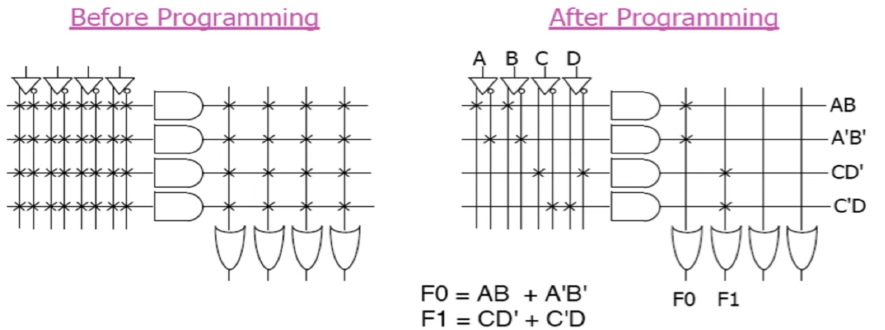
\includegraphics[width=0.86\linewidth]{bf.png}
\end{center}

\noindent Nella figura (a destra, dopo la programmazione) gli incroci segnati con $\times$
sono le connessioni rimaste. Con 4 ingressi $A,B,C,D$ il piano AND genera i 4 implicanti
$AB$, $\overline{A}\,\overline{B}$, $C\overline{D}$, $\overline{C}D$ e il piano OR li combina
nelle due funzioni:
\[
F_0 = AB + \overline{A}\,\overline{B} = \overline{A\oplus B}
\qquad\qquad
F_1 = C\overline{D} + \overline{C}D = C \oplus D
\]

\begin{important}
\textbf{PLA e ROM a confronto.} La ROM genera \emph{tutti} i $2^n$ mintermini e poi sceglie,
nel piano OR, quelli che servono: il piano AND è fisso e cresce esponenzialmente con $n$.
La PLA genera \emph{solo} i prodotti necessari e utili: anche il piano AND è programmabile e
il numero di righe è pari al numero di implicanti distinti (qui 4, contro i $2^4=16$
mintermini che servirebbero a una ROM). Per sfruttarla al meglio le funzioni vanno quindi
prima semplificate (ad esempio con le mappe di Karnaugh).
\end{important}

% ======================================================================
\section{Multiplexer e demultiplexer}

\subsection{Multiplexer (MUX)}

\begin{definizione}{MUX}
\textbf{MUX} (\emph{multiplexer}): circuito digitale che funziona similmente a un selettore,
con $2^n$ ingressi di dato, $n$ ingressi di indirizzo (linee di controllo) e 1 uscita.
L'uscita è uguale all'ingresso di dato il cui numero è scritto sugli indirizzi.
\end{definizione}

\noindent Un multiplexer con $2^n$ ingressi e $m$ uscite si indica con $2^n:m$
(ingressi : uscite); il MUX con una sola uscita è quindi un MUX $2^n:1$.

\begin{fitcenter}
\begin{circuitikz}[line width=0.6pt, font=\small, >=latex]
% simbolo generale
\draw[thick, fill=noteblue!4] (0,0) -- (1.2,0.6) -- (1.2,2.4) -- (0,3) -- cycle;
\node at (0.6,1.5) {MUX};
\foreach \y in {2.6,2.1,0.9,0.4}{ \draw[->] (-0.8,\y) -- (0,\y); }
\node at (-0.4,1.55) {$\vdots$};
\node[left, font=\scriptsize, align=right] at (-0.8,1.5) {$2^n$\\ingressi};
\draw[->] (1.2,1.5) -- (2.1,1.5) node[right, font=\scriptsize] {uscita $O$};
\draw[->, very thick] (0.6,-0.9) node[below, font=\scriptsize] {$n$ indirizzi} -- (0.6,0.3);
\node at (3.9,1.5) {$\Longrightarrow$};
% MUX 2:1 a porte
\begin{scope}[xshift=6.2cm]
\node[and port, scale=0.8] (A0) at (3.4,2.4) {};
\node[and port, scale=0.8] (A1) at (3.4,0.6) {};
\node[or port, scale=0.8] (O) at (5.2,1.5) {};
\draw (A0.out) -- ++(0.3,0) |- (O.in 1);
\draw (A1.out) -- ++(0.3,0) |- (O.in 2);
\draw[->] (O.out) -- ++(0.6,0) node[right] {$O$};
\draw (0,0 |- A0.in 1) node[left] {$a_0$} -- (A0.in 1);
\draw (0,0 |- A1.in 1) node[left] {$a_1$} -- (A1.in 1);
\draw (1.2,-0.7) node[below] {$S$} -- (1.2,0 |- A1.in 2) node[circle, fill, inner sep=1pt] {} -- (A1.in 2);
\draw (1.2,0 |- A1.in 2) -- (1.2,0 |- A0.in 2);
\node[not port, scale=0.5, anchor=in 1] (NS) at (1.5,0 |- A0.in 2) {};
\draw (1.2,0 |- A0.in 2) -- (NS.in 1);
\draw (NS.out) -- (A0.in 2);
\node[font=\scriptsize] at (3.4,-0.6) {MUX 2:1 ($n=1$)};
\end{scope}
\end{circuitikz}
\end{fitcenter}

\noindent Per $n=1$ il MUX si realizza con due AND e una OR:
$O = a_0\,\overline{S} + a_1\,S$. Se $S=0$ passa $a_0$, se $S=1$ passa $a_1$. In generale
ogni ingresso $a_k$ entra in una AND insieme al mintermine degli indirizzi che vale $k$, e le
AND sono raccolte da una OR: $O = \sum_k a_k\,m_k(S)$.

\medskip
\begin{important}
\textbf{Ogni funzione a $n$ variabili può essere implementata con un multiplexer
$2^{n-1}:1$.} Si usano $n-1$ variabili come indirizzi; per ogni combinazione degli indirizzi
la funzione, vista come funzione della variabile rimasta, può valere solo $0$, $1$, la
variabile stessa oppure la sua negazione, e questo valore si collega al corrispondente
ingresso di dato.
\end{important}

\noindent Consideriamo $F(a,b,c)=a\overline{b}+abc$ e costruiamo la \textbf{tabella di
verità funzionale} usando $a$ e $b$ come indirizzi di un MUX 4:1 ($2^{3-1}=4$ ingressi):
\begin{itemize}[leftmargin=1.5em, itemsep=1pt]
    \item $ab=00$ e $ab=01$: entrambi i termini contengono $a$, quindi $F=0$;
    \item $ab=10$: il primo termine vale 1, quindi $F=1$ (qualunque sia $c$);
    \item $ab=11$: resta solo il secondo termine, quindi $F=c$.
\end{itemize}

\begin{center}
\begin{minipage}[c]{0.3\linewidth}
\centering
\begin{tabular}{cc|c}
\toprule
$a$ & $b$ & $F$ \\
\midrule
0 & 0 & 0 \\
0 & 1 & 0 \\
1 & 0 & 1 \\
1 & 1 & $c$ \\
\bottomrule
\end{tabular}
\end{minipage}%
\begin{minipage}[c]{0.45\linewidth}
\centering
\begin{tikzpicture}[font=\small, >=latex, line width=0.6pt]
\draw[thick, fill=noteblue!4] (0,0) -- (1.4,0.6) -- (1.4,2.8) -- (0,3.4) -- cycle;
\node at (0.7,1.7) {\footnotesize MUX 4:1};
\foreach \v/\k/\y in {0/00/2.9, 0/01/2.2, 1/10/1.2, c/11/0.5}{
  \draw[->] (-1.0,\y) node[left] {$\v$} -- (0,\y);
  \node[right, font=\tiny] at (0,\y) {\k};
}
\draw[->] (1.4,1.7) -- (2.2,1.7) node[right] {$F$};
\draw[->] (0.45,-0.7) node[below] {$a$} -- (0.45,0.2);
\draw[->] (0.95,-0.7) node[below] {$b$} -- (0.95,0.42);
\end{tikzpicture}
\end{minipage}
\end{center}

\noindent Verifica: $F = \overline{a}\,\overline{b}\cdot 0 + \overline{a}\,b\cdot 0 +
a\,\overline{b}\cdot 1 + a\,b\cdot c = a\overline{b}+abc$.

\subsection{Demultiplexer (DEMUX)}

\begin{definizione}{DEMUX}
\textbf{DEMUX} (\emph{demultiplexer}): circuito digitale opposto al MUX, con 1 ingresso,
$n$ linee di controllo e $2^n$ uscite. L'ingresso viene inviato sull'uscita il cui numero è
scritto sugli indirizzi; tutte le altre uscite valgono 0.
\end{definizione}

\noindent Con la stessa notazione, un demultiplexer si indica con $m:2^n$ (qui $1:2^n$).

\begin{fitcenter}
\begin{circuitikz}[line width=0.6pt, font=\small, >=latex]
\draw[thick, fill=noteblue!4] (0,0.6) -- (1.6,0) -- (1.6,3) -- (0,2.4) -- cycle;
\node at (0.85,1.5) {\scriptsize DEMUX};
\draw[->] (-0.9,1.5) node[left, font=\scriptsize] {ingresso $I$} -- (0,1.5);
\foreach \y in {2.6,2.1,0.9,0.4}{ \draw[->] (1.6,\y) -- (2.4,\y); }
\node at (2.0,1.55) {$\vdots$};
\node[right, font=\scriptsize, align=left] at (2.4,1.5) {$2^n$\\uscite};
\draw[->, very thick] (0.8,-0.9) node[below, font=\scriptsize] {$n$ indirizzi} -- (0.8,0.35);
\node at (4.3,1.5) {$\Longrightarrow$};
\begin{scope}[xshift=6.2cm]
\node[and port, scale=0.8] (A1) at (3.4,2.4) {};
\node[and port, scale=0.8] (A0) at (3.4,0.6) {};
\draw[->] (A1.out) -- ++(0.6,0) node[right] {$o_1$};
\draw[->] (A0.out) -- ++(0.6,0) node[right] {$o_0$};
\draw (0,1.5) node[left] {$I$} -- (0.6,1.5) node[circle, fill, inner sep=1pt] {};
\draw (0.6,1.5) |- (A1.in 1);
\draw (0.6,1.5) |- (A0.in 1);
\draw (1.2,-0.7) node[below] {$S$} -- (1.2,0 |- A1.in 2) -- (A1.in 2);
\node[circle, fill, inner sep=1pt] at (1.2,0 |- A0.in 2) {};
\node[not port, scale=0.5, anchor=in 1] (NS) at (1.5,0 |- A0.in 2) {};
\draw (1.2,0 |- A0.in 2) -- (NS.in 1);
\draw (NS.out) -- (A0.in 2);
\node[font=\scriptsize] at (3.4,-0.6) {DEMUX 1:2 ($n=1$)};
\end{scope}
\end{circuitikz}
\end{fitcenter}

\noindent Per $n=1$: $o_0 = I\,\overline{S}$ e $o_1 = I\,S$. MUX e DEMUX si usano in coppia
per trasmettere più segnali su un'unica linea: il MUX sceglie quale segnale inviare, il DEMUX
all'altra estremità lo smista sull'uscita corretta (gli indirizzi dei due devono essere
sincronizzati).

% ======================================================================
\section{Universal Shift Register (USR)}

\begin{definizione}{USR}
\textbf{USR} (\emph{Universal Shift Register}): dispositivo che permette di inserire i dati in
parallelo o in serie e di spostarli a destra e a sinistra. Riunisce in un unico circuito
tutte le modalità dei registri a scorrimento (SISO, SIPO, PISO, PIPO).
\end{definizione}

\begin{center}
\begin{tikzpicture}[font=\small, >=latex, line width=0.6pt]
\foreach \x/\lab in {0/$n-1$, 2.6/$n$, 5.2/$n+1$}{
  \draw[thick, fill=noteblue!4] (\x,0) rectangle ++(1.6,1.2);
  \node at (\x+0.8,0.6) {\lab};
  \draw[->, green!50!black, thick] (\x+0.55,1.9) -- (\x+0.55,1.2);
  \draw[<-, green!50!black, thick] (\x+1.05,1.9) -- (\x+1.05,1.2);
}
\foreach \x in {-1,1.6,4.2,6.8}{
  \draw[->, red!70!black, thick] (\x,0.85) -- ++(1.0,0);
  \draw[<-, blue!70!black, thick] (\x,0.35) -- ++(1.0,0);
}
\node[font=\scriptsize, green!50!black] at (3.4,2.2) {ingresso / uscita parallela};
\node[font=\scriptsize, red!70!black, right] at (7.9,0.85) {shift right};
\node[font=\scriptsize, blue!70!black, right] at (7.9,0.35) {shift left};
\draw (-1,-0.5) node[left, font=\scriptsize] {$S_1S_0$} -- (6.8,-0.5);
\foreach \x in {0.8,3.4,6.0}{ \draw (\x,-0.5) node[circle, fill, inner sep=1pt] {} -- (\x,0); }
\end{tikzpicture}
\end{center}

\noindent Ogni cella $n$ è un flip-flop D che, a ogni fronte di clock, può caricare uno di
quattro valori: il proprio (hold), quello della cella di sinistra (shift right), quello
della cella di destra (shift left) o il dato parallelo $I_n$. Vediamo come implementare
ogni singola unità dell'USR.

\subsection{La cella elementare}

La scelta fra le quattro funzioni si fa con un \textbf{MUX 4:1}, i cui 2 indirizzi $S_1S_0$
sono comuni a tutte le celle:

\begin{center}
\begin{minipage}[c]{0.36\linewidth}
\centering
\begin{tabular}{cc|l|c}
\toprule
$S_1$ & $S_0$ & funzione & $D_n$ \\
\midrule
0 & 0 & hold & $Q_n$ \\
0 & 1 & shift right & $Q_{n-1}$ \\
1 & 0 & shift left & $Q_{n+1}$ \\
1 & 1 & data in & $I_n$ \\
\bottomrule
\end{tabular}
\end{minipage}%
\hspace{0.2cm}%
\begin{minipage}[c]{0.6\linewidth}
\centering
\begin{circuitikz}[line width=0.6pt, font=\small, >=latex]
\ctikzset{flipflops/scale=0.85}
\draw[thick, fill=noteblue!4] (0,0) -- (1.2,0.6) -- (1.2,2.8) -- (0,3.4) -- cycle;
\node at (0.6,1.7) {\footnotesize MUX};
\foreach \s/\k/\y in {Q_{n-1}/01/2.2, Q_{n+1}/10/1.2, I_n/11/0.5}{
  \draw (-0.9,\y) node[left, font=\scriptsize] {$\s$} -- (0,\y);
  \node[right, font=\tiny] at (0,\y) {\k};
}
\draw[->] (0.4,-0.7) node[below, font=\scriptsize] {$S_1$} -- (0.4,0.2);
\draw[->] (0.85,-0.7) node[below, font=\scriptsize] {$S_0$} -- (0.85,0.42);
\node[and port, scale=0.7] (AN) at (2.5,1.55) {};
\draw (1.2,1.7) -- (1.2,0 |- AN.in 1) -- (AN.in 1);
\node[not port, scale=0.5, rotate=90] (NC) at (1.7,0.5) {};
\draw (1.7,-0.7) node[below, font=\scriptsize] {CLR} -- (NC.in 1);
\draw (NC.out) |- (AN.in 2);
\node[flipflop D] (FF) at (4.3,1.8) {};
\draw (AN.out) -- ++(0.2,0) |- (FF.pin 1) node[above left, font=\scriptsize] {$D_n$};
\draw (FF.pin 3) -- ++(-0.3,0) -- ++(0,-1.6) node[below, font=\scriptsize] {CLK};
\draw[->] (FF.pin 6) -- ++(1.1,0) node[right, font=\scriptsize] {$Q_n$};
\node[right, font=\tiny] at (0,2.9) {00};
\draw (FF.pin 6) ++(0.5,0) node[circle, fill, inner sep=1pt] {} |- (-0.6,3.8) |- (0,2.9);
\node[above, font=\scriptsize] at (1.8,3.8) {$Q_n$ (hold)};
\end{circuitikz}
\end{minipage}
\end{center}

\noindent L'uscita del MUX passa per una porta AND il cui secondo ingresso è
$\overline{\text{CLR}}$: se $\text{CLR}=1$ si ha $D_n=0$ e al fronte di clock successivo il
flip-flop si azzera. Si tratta quindi di un \textbf{reset a 0 sincrono}. Si noti anche il
collegamento $Q_n\to$ ingresso 00, che realizza la funzione di hold.

\subsection{Implementazione a 4 bit}

Collegando quattro celle, l'ingresso 01 (shift right) di ogni cella riceve l'uscita della
cella a sinistra e l'ingresso 10 (shift left) quella della cella a destra. Le celle alle
estremità ricevono invece i due ingressi seriali:
\begin{itemize}[leftmargin=1.5em, itemsep=1pt]
    \item \textbf{RSI} (\emph{Right Serial Input}): entra nella cella $Q_0$ durante lo shift
          right; il dato esce da $Q_3$ (\textbf{RSO}, \emph{Right Serial Output});
    \item \textbf{LSI} (\emph{Left Serial Input}): entra nella cella $Q_3$ durante lo shift
          left; il dato esce da $Q_0$ (\textbf{LSO}, \emph{Left Serial Output}).
\end{itemize}

\begin{fitcenter}
\begin{tikzpicture}[font=\small, >=latex, line width=0.6pt]
\foreach \i in {0,1,2,3}{
  \node[draw, thick, fill=noteblue!4, minimum width=1.9cm, minimum height=1.4cm, align=center]
       (C\i) at (3.2*\i,0) {cella $\i$\\\scriptsize MUX + DFF};
  \draw[->] ($(C\i.north)+(-0.45,0.8)$) node[above] {$I_\i$} -- ($(C\i.north)+(-0.45,0)$);
  \draw[->] ($(C\i.north)+(0.45,0)$) -- ++(0,0.8) node[above] {$Q_\i$};
}
\foreach \i/\j in {0/1, 1/2, 2/3}{
  \draw[->, red!70!black] ($(C\i.east)+(0,0.3)$) -- ($(C\j.west)+(0,0.3)$);
  \draw[<-, blue!70!black] ($(C\i.east)+(0,-0.3)$) -- ($(C\j.west)+(0,-0.3)$);
}
\draw[->, red!70!black] ($(C0.west)+(-1.1,0.3)$) node[left] {RSI} -- ($(C0.west)+(0,0.3)$);
\draw[<-, blue!70!black] ($(C0.west)+(-1.1,-0.3)$) node[left] {LSO} -- ($(C0.west)+(0,-0.3)$);
\draw[->, red!70!black] ($(C3.east)+(0,0.3)$) -- ++(1.1,0) node[right] {RSO};
\draw[<-, blue!70!black] ($(C3.east)+(0,-0.3)$) -- ++(1.1,0) node[right] {LSI};
\foreach \s/\y in {$S_1S_0$/-1.3, CLK/-1.8, CLR/-2.3}{
  \draw (-2.0,\y) node[left, font=\scriptsize] {\s} -- (10.4,\y);
}
\foreach \i in {0,1,2,3}{
  \foreach \dx/\y in {-0.5/-1.3, 0/-1.8, 0.5/-2.3}{
    \draw ($(C\i.south)+(\dx,0)$) -- ($(C\i.south)+(\dx,0)$ |- 0,\y) node[circle, fill, inner sep=1pt] {};
  }
}
\end{tikzpicture}
\end{fitcenter}

\noindent Con lo stesso circuito si ottengono tutte le modalità: caricamento parallelo
($S_1S_0=11$), shift right (01), shift left (10) e hold (00). Ad esempio, per una
trasmissione \textbf{PISO} si carica il dato con $S_1S_0=11$ e poi lo si fa uscire un bit
alla volta con lo shift; per una ricezione \textbf{SIPO} si fanno entrare i bit dall'ingresso
seriale e si leggono le uscite $Q_0\ldots Q_3$.

\subsection{Applicazione: trasmissione seriale Sender--Receiver}

Due USR a 8 bit (ciascuno formato da due integrati a 4 bit in cascata) permettono di
trasmettere un byte su un'unica linea. Il trasmettitore (\emph{Sender}) lavora in modalità
PISO, il ricevitore (\emph{Receiver}) in modalità SIPO; i due condividono il clock.

\begin{fitcenter}
\begin{tikzpicture}[font=\small, >=latex, line width=0.6pt]
\node[draw, thick, fill=noteblue!4, minimum width=3.4cm, minimum height=1.5cm, align=center] (S) at (0,0)
     {\textbf{Sender}\\\scriptsize USR 8 bit (PISO)};
\node[draw, thick, fill=noteblue!4, minimum width=3.4cm, minimum height=1.5cm, align=center] (R) at (7.4,0)
     {\textbf{Receiver}\\\scriptsize USR 8 bit (SIPO)};
\foreach \k in {0,...,7}{
  \draw[->] ($(S.north west)+(0.35+0.385*\k,0.6)$) -- ($(S.north west)+(0.35+0.385*\k,0)$);
  \draw[->] ($(R.north west)+(0.35+0.385*\k,0)$) -- ($(R.north west)+(0.35+0.385*\k,0.6)$);
}
\node[above] at ($(S.north)+(0,0.6)$) {$D_1\ldots D_8$ (dati da trasmettere)};
\node[above] at ($(R.north)+(0,0.6)$) {$D_1\ldots D_8$ (dati ricevuti)};
\draw[->, very thick, notered] (S.east) -- node[above, font=\scriptsize] {linea seriale}
     node[below, font=\scriptsize, black] {LSO $\to$ LSI} (R.west);
\draw (-2.6,-1.4) node[left, font=\scriptsize] {Clock} -- (7.4,-1.4);
\draw[->] (0,-1.4) node[circle, fill, inner sep=1pt] {} -- (S.south);
\draw[->] (7.4,-1.4) -- (R.south);
\draw[->] ($(S.south)+(-1.2,-0.9)$) node[below, font=\scriptsize] {$S_1S_0$} -- ($(S.south)+(-1.2,0)$);
\draw[->] ($(R.south)+(-1.2,-0.9)$) node[below, font=\scriptsize] {$S_1S_0$} -- ($(R.south)+(-1.2,0)$);
\end{tikzpicture}
\end{fitcenter}

\noindent Il flusso dell'operazione è:
\begin{enumerate}[leftmargin=1.8em, itemsep=2pt]
    \item \textbf{caricamento nel Sender} dei dati $D_i$: $S_1S_0=11$ sul Sender, un colpo di
          clock;
    \item \textbf{trasmissione sulla linea seriale}: Sender e Receiver entrambi in shift
          ($S_1S_0=10$); a ogni colpo di clock un bit esce dall'uscita seriale del Sender ed
          entra nell'ingresso seriale del Receiver. Dopo 8 colpi di clock l'intero byte è
          stato trasferito;
    \item \textbf{lettura sulle uscite del Receiver}: il Receiver viene messo in hold
          ($S_1S_0=00$) e i dati $D_1\ldots D_8$ sono disponibili in parallelo.
\end{enumerate}
Il vantaggio è che servono solo una linea dati (più il clock e la massa) invece di otto.

% ======================================================================
\section{Vincoli temporali dell'USR e jitter}

Il clock di un USR non può essere arbitrariamente veloce: fra due fronti consecutivi il
segnale deve uscire da un flip-flop, attraversare il MUX della cella successiva e arrivare
stabile all'ingresso $D$ in tempo per il fronte seguente. La \textbf{massima frequenza del
clock} corrisponde quindi al \textbf{minimo periodo del clock}:

\[
\boxed{T_{\text{CLK,min}} = T_{\text{propag}} + T_{\text{lc}} + T_{\text{setup}} + T_{\text{jitter}}}
\qquad\qquad f_{\text{CLK,max}} = \frac{1}{T_{\text{CLK,min}}}
\]

\begin{itemize}[leftmargin=1.5em, itemsep=1pt]
    \item $T_{\text{propag}}$: ritardo CLK$\to Q$ nel flip-flop;
    \item $T_{\text{lc}}$: ritardo nella logica combinatoria (il MUX e la porta AND);
    \item $T_{\text{setup}}$: tempo per cui $D$ deve restare stabile prima del clock
          successivo;
    \item $T_{\text{jitter}}$: margine per l'incertezza sull'istante di arrivo del fronte.
\end{itemize}

\begin{center}
\begin{tikzpicture}[x=1cm, y=1cm, font=\scriptsize, line width=0.6pt, >=latex]
\node[left] at (-0.2,2.3) {CLK};
\draw (-0.2,2) -- (0,2) -- (0,2.6) -- (1.5,2.6) -- (1.5,2) -- (9,2) -- (9,2.6) -- (10.2,2.6);
\fill[red!20] (8.6,1.9) rectangle (9.4,2.7);
\draw (9,2) -- (9,2.6);
\node[left] at (-0.2,1.1) {$Q_{n-1}$};
\draw (-0.2,0.8) -- (2,0.8) -- (2.15,1.4) -- (10.2,1.4);
\draw (-0.2,1.4) -- (2,1.4) -- (2.15,0.8) -- (10.2,0.8);
\node[left] at (-0.2,-0.1) {$D_n$};
\draw (-0.2,-0.4) -- (5.2,-0.4) -- (5.35,0.2) -- (10.2,0.2);
\draw (-0.2,0.2) -- (5.2,0.2) -- (5.35,-0.4) -- (10.2,-0.4);
\foreach \x in {0,2.1,5.3,7.6,9}{ \draw[dashed, gray] (\x,-1.0) -- (\x,2.8); }
\draw[<->, teal] (0,-0.8) -- node[below] {$T_{\text{propag}}$} (2.1,-0.8);
\draw[<->, orange!90!black] (2.1,-0.8) -- node[below] {$T_{\text{lc}}$} (5.3,-0.8);
\draw[<->, blue] (7.6,-0.8) -- node[below] {$T_{\text{setup}}$} (9,-0.8);
\draw[<->, red] (8.6,3.0) -- node[above] {$T_{\text{jitter}}$} (9.4,3.0);
\draw[<->] (0,-1.7) -- node[below] {$T_{\text{CLK}} \ge T_{\text{CLK,min}}$} (9,-1.7);
\node[align=center] at (6.45,-0.25) {\tiny margine};
\end{tikzpicture}
\end{center}

\begin{definizione}{Jitter del CLK}
$\Delta_{\max}$ fra gli istanti di arrivo dei fronti di clock che dovrebbero giungere
\emph{contemporaneamente} a tutti i componenti del circuito, ma che in pratica non lo fanno a
causa di variazioni fisiche (diversa lunghezza dei percorsi, carichi diversi, rumore,
variazioni di temperatura).
\end{definizione}

\noindent Se il fronte arriva alla cella successiva in anticipo rispetto a quello della cella
precedente, il tempo disponibile si riduce: per questo il jitter va sommato agli altri
ritardi nel calcolo di $T_{\text{CLK,min}}$.

% ======================================================================
\chapter{Conversione Digitale--Analogica e Analogica--Digitale}
\textit{(15 maggio 2026)}

% ======================================================================
\section{Conversione digitale $\leftrightarrow$ analogica}

Le grandezze fisiche (temperatura, pressione, suono, \ldots) sono analogiche, mentre la loro
elaborazione avviene quasi sempre in digitale. Un sistema di acquisizione, come l'Analog
Discovery 2 (AD2) usato in laboratorio, trasforma quindi la tensione fornita da un sensore in
una sequenza di numeri e, se serve, ricostruisce poi un segnale analogico:

\begin{fitcenter}
\begin{tikzpicture}[font=\small, >=latex, line width=0.6pt,
  blocco/.style={draw, thick, minimum width=1.6cm, minimum height=0.9cm, align=center, fill=noteblue!4}]
% segnale campionato
\draw[->] (0,0) -- (3.2,0) node[right] {$t$};
\draw[->] (0,0) -- (0,2.0) node[above] {$V$};
\foreach \x/\y in {0.4/1.2, 0.8/0.8, 1.2/0.6, 1.6/0.9, 2.0/1.3, 2.4/1.6, 2.8/1.5}{
  \node[font=\footnotesize, text=noteblue] at (\x,\y) {$\times$};
}
\node[font=\scriptsize] at (1.6,2.75) {campionamenti $V(t_i)$};
% blocchi
\node[blocco] (sen) at (4.8,1.0) {Sensore};
\node[blocco] (adc) at (7.4,1.0) {ADC\\\scriptsize(es. AD2)};
\node[blocco] (el)  at (10.2,1.0) {elaborazione\\digitale};
\node[blocco] (dac) at (13.0,1.0) {DAC};
\draw[->, thick] (sen) -- node[above, font=\scriptsize] {$V_{\text{in}}$} (adc);
\draw[->, thick] (adc) -- node[above, font=\scriptsize] {$n_{\text{out}}$} (el);
\draw[->, thick] (el) -- node[above, font=\scriptsize] {$n_{\text{in}}$} (dac);
% segnale ricostruito
\begin{scope}[xshift=14.6cm]
\draw[->] (0,0) -- (3.2,0) node[right] {$t$};
\draw[->] (0,0) -- (0,2.0) node[above] {$V$};
\draw[thick, noteblue] (0.4,1.2) -- (0.8,0.8) -- (1.2,0.6) -- (1.6,0.9) -- (2.0,1.3) -- (2.4,1.6) -- (2.8,1.5);
\foreach \x/\y in {0.4/1.2, 0.8/0.8, 1.2/0.6, 1.6/0.9, 2.0/1.3, 2.4/1.6, 2.8/1.5}{
  \node[font=\footnotesize, text=noteblue] at (\x,\y) {$\times$};
}
\node[font=\scriptsize, align=center] at (1.8,2.9) {ricostruzione (interpolazione lineare)};
\end{scope}
\draw[->, thick] (dac.east) -- (14.5,1.0);
\end{tikzpicture}
\end{fitcenter}

\noindent Che cosa succede fra il sensore e il segnale ricostruito? La catena è:
\begin{align*}
&\text{\textbf{sample and hold}} \;\longrightarrow\; \text{\textbf{convertitore analogico--digitale (ADC)}} \;\longrightarrow\\
&\longrightarrow\; \text{elaborazione digitale} \;\longrightarrow\; \text{\textbf{convertitore digitale--analogico (DAC)}}
\end{align*}
Il \emph{sample and hold} preleva il valore della tensione in un istante $t_i$ e lo mantiene
costante per tutto il tempo necessario alla conversione; l'ADC lo trasforma in un numero;
dopo l'elaborazione il DAC riporta i numeri in tensioni, che vengono raccordate
(nel caso più semplice con segmenti di retta).

\medskip
\noindent Definizioni di base, per un convertitore a $N$ bit:
\begin{itemize}[leftmargin=1.5em, itemsep=2pt]
    \item $n$ = numero intero che dipende dai bit disponibili: $0 \le n \le 2^N-1$;
    \item $\Delta V$ = \textbf{granularità}, cioè il passo minimo distinguibile (la tensione
          che corrisponde a 1 LSB);
    \item $V_{\text{ref}}$ = tensione di riferimento, cioè il \textbf{valore massimo
          ottenibile} (il fondo scala). Non va confusa con $\Delta V$: i due sono legati da
          \[
          \Delta V = \frac{V_{\text{ref}}}{2^N}
          \]
\end{itemize}

\begin{definizione}{Funzioni di trasferimento}
\textbf{ADC}: \quad $n_{\text{out}} = \dfrac{V_{\text{in}}}{\Delta V}$ \quad (arrotondato a un
numero intero)\\[0.6em]
\textbf{DAC}: \quad $V_{\text{out}} = n_{\text{in}} \cdot \Delta V$
\end{definizione}

% ======================================================================
\section{Caratteristiche del DAC}

\begin{definizione}{Precisione}
determinata dal numero di bit e dall'intervallo di tensioni: $V_{\text{out}} = n_{\text{in}}\,\Delta V$.
\end{definizione}

\noindent Ad esempio, con $N=3$ bit e $\Delta V = 1\,\text{V}$:
$n_{\text{in}} \in [0,\, 2^3-1] = [0,7] \;\Rightarrow\; V_{\text{out}} \in [0,\,7]\,\text{V}$,
con passi da 1\,V. A parità di intervallo, aumentare il numero di bit riduce $\Delta V$ e
rende l'uscita più fine.

\medskip
\noindent La \textbf{velocità di conversione} è molto importante e dipende da vari fattori:
il \textbf{tempo di assestamento} dell'uscita dopo un cambio del codice, l'\textbf{architettura}
del convertitore e il \textbf{numero di bit} (più bit, in genere, significano una
conversione più lenta).

\medskip
\noindent Il comportamento reale di un DAC si discosta da quello ideale per tre principali
sorgenti di errore:

\begin{center}
\begin{minipage}[t]{0.32\linewidth}\centering
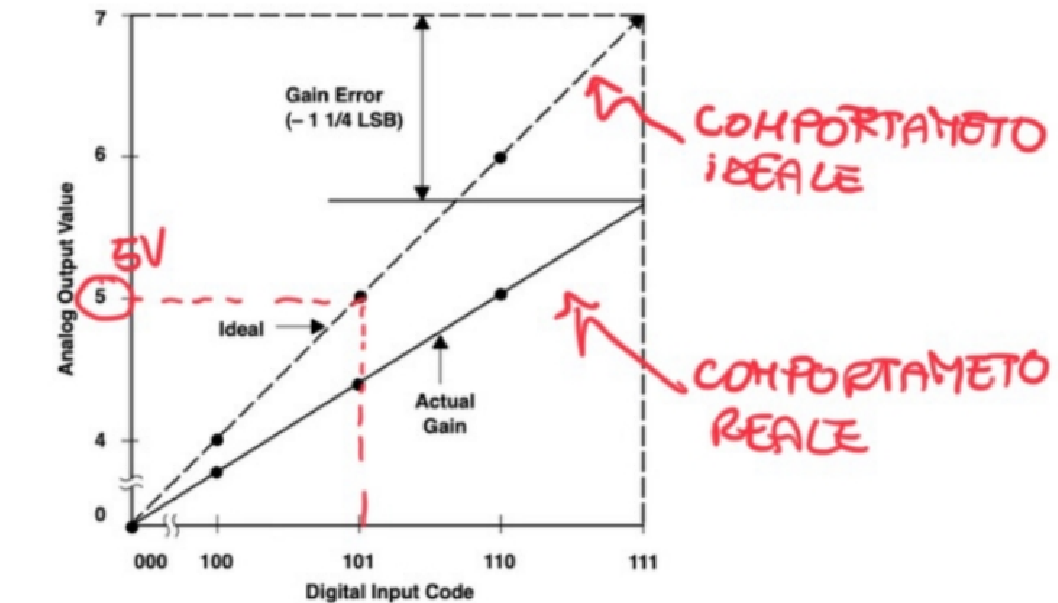
\includegraphics[width=\linewidth]{err_g.png}\\
\footnotesize (a) errore di guadagno
\end{minipage}\hfill
\begin{minipage}[t]{0.32\linewidth}\centering
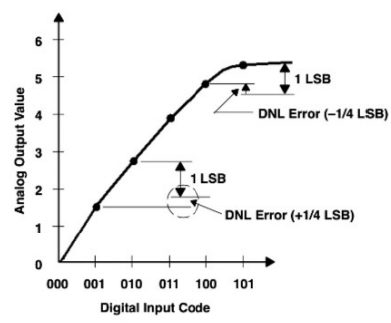
\includegraphics[width=\linewidth]{n_lin.png}\\
\footnotesize (b) non linearità
\end{minipage}\hfill
\begin{minipage}[t]{0.32\linewidth}\centering
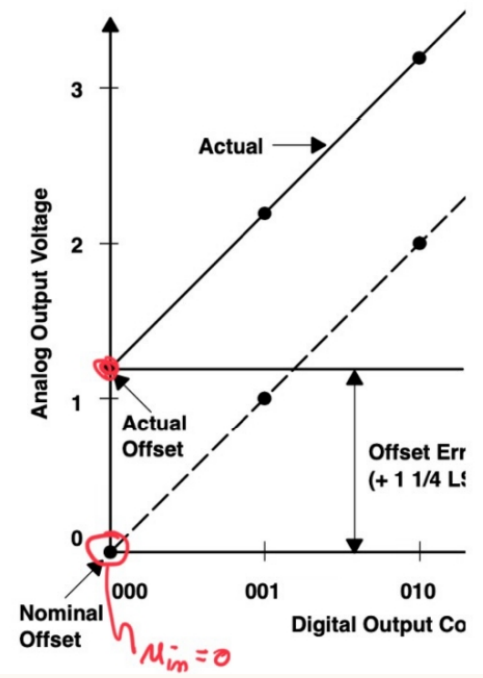
\includegraphics[width=\linewidth]{er_nlin.png}\\
\footnotesize (c) errore di offset
\end{minipage}
\end{center}

\begin{itemize}[leftmargin=1.5em, itemsep=2pt]
    \item \textbf{(a) Errore di guadagno}: la caratteristica reale è una retta con pendenza
          diversa da quella ideale; l'errore cresce con il codice ed è massimo a fondo scala.
    \item \textbf{(b) Non linearità}: i gradini non sono tutti uguali, per cui la
          caratteristica si incurva. La non linearità differenziale (DNL) misura quanto ogni
          singolo passo differisce da 1 LSB.
    \item \textbf{(c) Errore di offset}: la caratteristica è traslata; per $n_{\text{in}}=0$
          l'uscita non vale 0 e l'errore è lo stesso per tutti i codici.
\end{itemize}

% ======================================================================
\section{DAC a sommatore}

L'architettura più semplice di DAC è il \textbf{DAC a sommatore pesato}: un amplificatore
operazionale in configurazione invertente somma le correnti di più resistenze di ingresso,
una per bit. Ogni resistenza è collegata a $V_{\text{ref}}$ se il bit vale $a_i=1$ oppure a
massa se $a_i=0$, tramite uno \textbf{switch} comandato dal bit.

\begin{fitcenter}
\begin{circuitikz}[line width=0.6pt, font=\small, american]
\node[op amp, anchor=-] (OA) at (6.2,1.4) {};
\draw (OA.+) -- ++(-0.4,0) node[ground] {};
\coordinate (S) at (5.2,1.4);
\draw (S) -- (OA.-);
\draw (S) -- (S |- 0,-1.4);
\draw (S) -- (S |- 0,3.0) to[R, l=$R$] (OA.out |- 0,3.0) -- (OA.out);
\draw (OA.out) to[short, -o] ++(0.8,0) node[right] {$V_{\text{out}}$};
\foreach \i/\y/\r/\lab in {2/1.4/{R/4}/MSB, 1/0/{R/2}/, 0/-1.4/R/LSB}{
  \draw (S |- 0,\y) node[circle, fill, inner sep=1pt] {} to[R, l=$\r$] (1.6,\y) coordinate (P\i);
  \draw (P\i) node[circle, fill, inner sep=1pt] {} -- (0.9,\y+0.3);
  \draw (0.8,\y+0.4) node[circle, draw, fill=white, inner sep=1pt] {} -- (0.2,\y+0.4) node[left, font=\scriptsize] {$V_{\text{ref}}$};
  \draw (0.8,\y-0.4) node[circle, draw, fill=white, inner sep=1pt] {} -- (0.2,\y-0.4) node[ground, scale=0.6] {};
  \node[font=\scriptsize, color=noteblue, anchor=north west] at (1.1,\y-0.05) {$a_\i$};
  \node[font=\scriptsize, color=noteblue, anchor=east] at (-0.6,\y) {\lab};
}
\end{circuitikz}
\end{fitcenter}

\noindent Poiché l'ingresso invertente è una massa virtuale, ogni ramo porta una corrente
indipendente dagli altri, $I_i = a_i V_{\text{ref}}/R_i$, e tutte le correnti attraversano la
resistenza di retroazione $R$. Per sovrapposizione degli effetti (qui con tutti i bit a 1):
\[
V_{\text{out}} = -V_{\text{ref}}\left(\frac{R}{R_0}+\frac{R}{R_1}+\frac{R}{R_2}\right)
\]
Scegliendo resistenze pesate $R_i = R/2^i$ si ha $R/R_i = 2^i$ e quindi
$V_{\text{out}} = -V_{\text{ref}}\sum_i 2^i$. Considerando gli switch, ogni bit vale
$a_i=0$ (collegamento a massa) oppure $a_i=1$ (collegamento a $V_{\text{ref}}$):
\[
\boxed{V_{\text{out}} = -V_{\text{ref}}\sum_{i=0}^{N-1} a_i\,2^i}
\]
Il bit più significativo ha la resistenza più piccola ($R/2^{N-1}$) e quindi il peso
maggiore. Con 3 bit e ingresso $101_2$: $V_{\text{out}} = -V_{\text{ref}}(4+1) = -5\,V_{\text{ref}}$.

\begin{important}
\textbf{Limite pratico.} Supponiamo di avere 10 bit con $R_i = 100\,\text{k}\Omega/2^i$: le
resistenze vanno da $100\,\text{k}\Omega$ (LSB) a circa $98\,\Omega$ (MSB).
\begin{itemize}[leftmargin=1.3em, itemsep=2pt]
    \item Se la tolleranza vale $\sigma_0 = 1\%$ di $R_0 = 100\,\text{k}\Omega$, cioè
          $\sigma_0 = 1\,\text{k}\Omega$, e l'incertezza assoluta è la stessa per tutte le
          resistenze, quelle dei bit più pesanti sono addirittura più piccole
          dell'incertezza ($R_i < \sigma_0$ per $i \ge 7$: $R_7 \approx 781\,\Omega$).
    \item Anche con una tolleranza relativa dell'1\% su ogni resistenza, il bit più
          significativo pesa $2^9=512$ volte l'LSB e il suo errore vale circa $5$ LSB, molto
          più del contributo dei bit meno significativi. Questi bit vengono quindi
          \textbf{persi}: per non perderli servirebbe una tolleranza inferiore a
          $1/2^N$ (circa $0{,}1\%$ per 10 bit).
    \item Resistenze con valori così diversi sono difficili da realizzare con la stessa
          precisione, soprattutto in un circuito integrato.
\end{itemize}
Il DAC a sommatore si può quindi usare solo se abbiamo pochi bit, altrimenti non è utile.
\end{important}

% ======================================================================
\section{DAC R-2R Ladder}

Per avere un DAC più preciso si usa la tecnica \textbf{R-2R Ladder} (rete a scala), che
genera pesi binari per i bit usando \textbf{solo due valori di resistenza}, $R$ e $2R$.
È molto più facile ottenere resistenze tutte uguali (e con errori correlati) che resistenze
di valori molto diversi.

\begin{fitcenter}
\begin{circuitikz}[line width=0.6pt, font=\small, american]
% nodi della scala: MSB in alto
\foreach \i/\y in {0/4.5, 1/3.0, 2/1.5, 3/0}{
  \coordinate (N\i) at (4,\y);
  \draw (N\i) node[circle, fill, inner sep=1.2pt] {} to[R, l_=$2R$] (1.6,\y) coordinate (P\i);
  \draw (P\i) node[circle, fill, inner sep=1pt] {} -- (0.9,\y+0.3);
  \draw (0.8,\y+0.4) node[circle, draw, fill=white, inner sep=1pt] {} -- (0.2,\y+0.4) node[left, font=\scriptsize] {$V_{\text{ref}}$};
  \draw (0.8,\y-0.4) node[circle, draw, fill=white, inner sep=1pt] {} -- (0.2,\y-0.4) node[ground, scale=0.6] {};
  \node[font=\scriptsize, color=noteblue, anchor=north west] at (1.1,\y-0.05) {$a_\i$};
}
\draw (N0) to[R, l=$R$] (N1) to[R, l=$R$] (N2) to[R, l=$R$] (N3);
\draw (N3) to[R, l=$2R$] (4,-1.6) node[ground] {};
\node[font=\scriptsize, color=noteblue, anchor=east] at (-0.6,4.5) {MSB};
\node[font=\scriptsize, color=noteblue, anchor=east] at (-0.6,0) {LSB};
% amplificatore
\node[op amp, anchor=-] (OA) at (6.6,4.5) {};
\draw (N0) -- (OA.-);
\draw (OA.+) -- ++(-0.4,0) node[ground] {};
\draw (5.6,0 |- OA.-) node[circle, fill, inner sep=1.2pt] {} -- (5.6,5.8) to[R, l=$R$] (OA.out |- 0,5.8) -- (OA.out);
\draw (OA.out) to[short, -o] ++(0.8,0) node[right] {$V_{\text{out}}$};
\end{circuitikz}
\end{fitcenter}

\noindent\textbf{Perché i pesi sono binari.} Guardando verso il basso da un qualsiasi nodo, la
parte di scala sottostante ha resistenza equivalente $2R$ (partendo dal fondo:
$2R \parallel 2R = R$, in serie a $R$ dà di nuovo $2R$, e così via). A ogni nodo, quindi, il
contributo di tensione di un bit viene diviso per 2 salendo di un gradino. Ne segue che il
bit $a_i$ ($i=0$ MSB) contribuisce all'uscita con
\[
a_i \;\longrightarrow\; V_{\text{out},i} = -\frac{V_{\text{ref}}}{2^{i+1}}
\qquad\Rightarrow\qquad \text{i pesi sono } \frac{1}{2},\,\frac{1}{4},\,\frac{1}{8},\,\frac{1}{16},\,\ldots
\]
e sommando tutti i contributi:
\[
\boxed{V_{\text{out}} = -V_{\text{ref}}\sum_{i=0}^{N-1} \frac{a_i}{2^{i+1}}}
\]
L'uscita massima (tutti i bit a 1) vale $-V_{\text{ref}}(1-2^{-N})$, cioè il fondo scala meno
un LSB, e il passo è $\Delta V = V_{\text{ref}}/2^N$.

\begin{esercizio}{Esempio}
Con 4 bit, ingresso $a_0a_1a_2a_3 = 1010$ e $V_{\text{ref}} = 8\,\text{V}$:
\[
V_{\text{out}} = -8\left(\frac{1}{2}+\frac{1}{8}\right) = -8 \cdot \frac{5}{8} = -5\,\text{V}
\]
In modulo il risultato coincide con $n_{\text{in}}\,\Delta V = 10 \cdot \frac{8}{16} = 5\,\text{V}$.
\end{esercizio}

\begin{osservazione}{Scelta delle resistenze di terminazione e di retroazione}
Negli appunti la terminazione in fondo alla scala è indicata come $R$ e la resistenza di
retroazione come $2R$. Risolvendo il circuito (nodo MSB a massa virtuale) con le quattro
combinazioni possibili si ottiene, per l'esempio $1010$ con $V_{\text{ref}}=8$\,V:
\begin{center}
\small\renewcommand{\arraystretch}{1.6}
\begin{tabular}{c|c|c|c}
\toprule
terminazione & retroazione & pesi dei bit $a_0,a_1,a_2,a_3$ & $V_{\text{out}}(1010)$ \\
\midrule
$R$  & $2R$ & $1,\ \tfrac{42}{85},\ \tfrac{4}{17},\ \tfrac{8}{85}$ & $-9{,}88$\,V \\
$R$  & $R$  & $\tfrac12,\ \tfrac{21}{85},\ \tfrac{2}{17},\ \tfrac{4}{85}$ & $-4{,}94$\,V \\
$2R$ & $2R$ & $1,\ \tfrac12,\ \tfrac14,\ \tfrac18$ & $-10$\,V \\
$\mathbf{2R}$ & $\mathbf{R}$ & $\tfrac12,\ \tfrac14,\ \tfrac18,\ \tfrac1{16}$ & $\mathbf{-5}$\,\textbf{V} \\
\bottomrule
\end{tabular}
\end{center}
\begin{itemize}[leftmargin=1.3em, itemsep=1pt]
    \item Con terminazione $R$ i pesi \textbf{non sono più potenze di 2}: la scala vede
          verso il basso una resistenza diversa da $2R$ e la divisione per 2 a ogni nodo
          non vale più. La terminazione deve quindi essere $2R$.
    \item La retroazione fissa solo il guadagno: con $2R$ tutte le uscite raddoppiano.
          Il risultato degli appunti ($5$\,V, cioè pesi $\tfrac12,\tfrac14,\ldots$) si
          ottiene solo con retroazione $R$, uguale alla resistenza equivalente della scala.
\end{itemize}
Lo schema e le formule di questa sezione usano quindi terminazione $2R$ e retroazione $R$.
\end{osservazione}

% ======================================================================
\section{Caratteristiche dell'ADC}

\begin{itemize}[leftmargin=1.5em, itemsep=2pt]
    \item \textbf{Accuratezza}: insieme di tutte le sorgenti di errore; comprende sempre
          almeno l'errore di quantizzazione.
    \item \textbf{Errore di quantizzazione}: dipende dal tipo di ADC ed è dovuto alla
          discretizzazione del segnale durante la conversione. Tutte le tensioni che cadono
          nello stesso gradino producono lo stesso codice, quindi l'informazione all'interno
          di un gradino è persa. Di solito vale $1$ LSB (se il codice è ottenuto per
          troncamento) oppure $\pm 0{,}5$ LSB (se i gradini sono centrati sui valori ideali).
    \item \textbf{Tempo di conversione} e \textbf{principio di funzionamento} sono le altre
          caratteristiche importanti (i diversi tipi di ADC sono trattati nel capitolo
          successivo).
\end{itemize}

\begin{center}
\begin{tikzpicture}[x=0.75cm, y=0.55cm, font=\scriptsize, line width=0.6pt, >=latex]
\draw[->] (0,0) -- (8.6,0) node[right] {$V_{\text{in}}/\Delta V$};
\draw[->] (0,0) -- (0,8) node[above] {$n_{\text{out}}$};
\draw[dashed, gray] (0,0) -- (8,8);
\draw[thick, noteblue] (0,0) \foreach \k in {0,...,6}{ -- (\k+0.5,\k) -- (\k+0.5,\k+1) } -- (8,7);
\foreach \k in {0,...,7}{ \node[left] at (0,\k) {\k}; }
\foreach \k in {0,...,8}{ \node[below] at (\k,0) {\k}; }
\begin{scope}[yshift=-2.6cm]
\draw[->] (0,0) -- (8.6,0) node[right] {$V_{\text{in}}/\Delta V$};
\draw[->] (0,-1.2) -- (0,1.4) node[above] {errore};
\draw[thick, notered] (0,0) \foreach \k in {0,...,6}{ -- (\k+0.5,-0.5*1.6) -- (\k+0.5,0.5*1.6) } -- (7.5,-0.8);
\node[left] at (0,0.8) {$+\frac{1}{2}$ LSB};
\node[left] at (0,-0.8) {$-\frac{1}{2}$ LSB};
\end{scope}
\end{tikzpicture}
\end{center}

\noindent Nella figura (ADC ideale a 3 bit con gradini centrati) la caratteristica a gradini
approssima la retta ideale tratteggiata; la differenza fra le due è l'errore di
quantizzazione, un ``dente di sega'' compreso fra $-\frac12$ e $+\frac12$ LSB.

\medskip
\noindent Analogamente al DAC, anche l'ADC presenta tre principali tipi di errore rispetto
al comportamento ideale (linea tratteggiata = ADC ideale, linea continua = ADC reale):

\begin{center}
\begin{minipage}[t]{0.32\linewidth}\centering
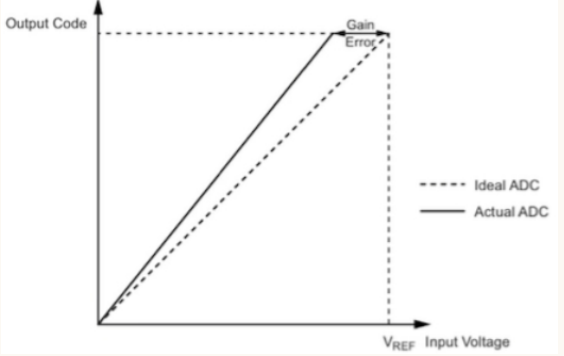
\includegraphics[width=\linewidth]{err_g2.png}\\
\footnotesize (a) errore di guadagno
\end{minipage}\hfill
\begin{minipage}[t]{0.32\linewidth}\centering
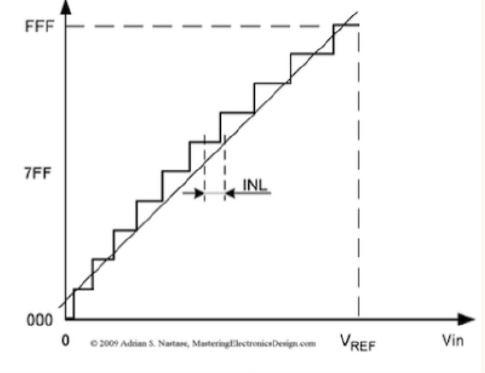
\includegraphics[width=\linewidth]{n_lin2.png}\\
\footnotesize (b) non linearità integrale (INL)
\end{minipage}\hfill
\begin{minipage}[t]{0.32\linewidth}\centering
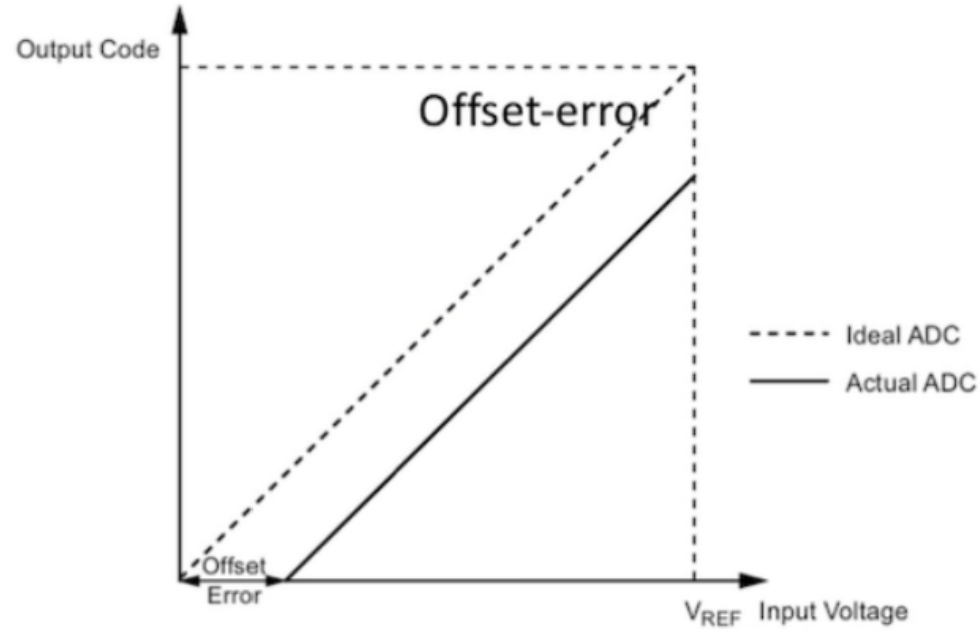
\includegraphics[width=\linewidth]{er_nlin2.png}\\
\footnotesize (c) errore di offset
\end{minipage}
\end{center}

\begin{itemize}[leftmargin=1.5em, itemsep=2pt]
    \item \textbf{(a) Errore di guadagno}: la pendenza della caratteristica reale è diversa da
          quella ideale, per cui il codice massimo viene raggiunto a una tensione diversa da
          $V_{\text{ref}}$.
    \item \textbf{(b) Non linearità integrale (INL)}: massima distanza fra la caratteristica a
          gradini reale e la retta ideale, lungo tutto l'intervallo di ingresso.
    \item \textbf{(c) Errore di offset}: la caratteristica è traslata, per cui la prima
          transizione avviene a una tensione diversa da quella ideale.
\end{itemize}

% ======================================================================
\chapter{Convertitori Analogico-Digitali (ADC)}
\textit{(15 maggio 2026 -- cont.)}

\noindent Un ADC deve trovare il codice $n_{\text{out}}$ tale che $n_{\text{out}}\,\Delta V$
approssimi la tensione di ingresso. Le architetture più comuni si distinguono per
\emph{come} cercano questo codice: provando tutti i valori in ordine (ADC a gradinata),
con una ricerca binaria (ADC ad approssimazioni successive) oppure confrontando la tensione
con tutti i livelli contemporaneamente (Flash ADC). Le prime due architetture contengono al
loro interno un DAC, che genera la tensione di confronto.

% ======================================================================
\section{ADC a gradinata}

\begin{fitcenter}
\begin{circuitikz}[line width=0.6pt, font=\small, >=latex, american]
% comparatore
\node[op amp] (CMP) at (3.2,3.0) {};
\draw (CMP.-) -- ++(-1.2,0) node[left] {$X$ \scriptsize(tensione da misurare)};
\node[font=\scriptsize] at (3.2,4.1) {comparatore};
% latch RS
\node[draw, thick, fill=noteblue!4, minimum width=1.3cm, minimum height=1.5cm] (L) at (6.2,3.0) {};
\node[anchor=west, font=\scriptsize] at ($(L.west)+(0,0.4)$) {S};
\node[anchor=west, font=\scriptsize] at ($(L.west)+(0,-0.4)$) {R};
\node[anchor=east, font=\scriptsize] at ($(L.east)+(0,0.4)$) {Q};
\node[anchor=east, font=\scriptsize] at ($(L.east)+(0,-0.4)$) {$\overline{\text{Q}}$};
\node[above, font=\scriptsize] at (L.north) {latch RS};
\draw (CMP.out) -- ++(0.4,0) |- ($(L.west)+(0,0.4)$);
\draw[->] ($(L.east)+(0,0.4)$) -- ++(1.4,0) node[right] {EoC};
\node[font=\scriptsize, anchor=west] at (8.1,3.05) {(\emph{End of Conversion})};
% DAC
\node[draw, thick, fill=noteblue!4, minimum width=1.6cm, minimum height=0.9cm] (DAC) at (1.8,1.3) {DAC};
\draw (DAC.north) |- (CMP.+) node[pos=0.3, left, font=\scriptsize] {$Y_{\text{DAC}}$};
% contatore
\node[draw, thick, fill=noteblue!4, minimum width=1.8cm, minimum height=0.9cm] (CNT) at (1.8,-0.4) {contatore};
\draw[->, very thick] (CNT.north) -- node[right, font=\scriptsize] {$n$ bit} (DAC.south);
\draw[->, very thick] ($(CNT.north)+(-0.5,0.4)$) -- ++(-1.6,0) node[left] {$Y$};
\node[circle, fill, inner sep=1.4pt] at ($(CNT.north)+(0,0.4)$) {};
\draw[very thick] ($(CNT.north)+(0,0.4)$) -- ++(-0.5,0);
% porta AND sul clock (uscita a sinistra, verso il contatore)
\node[and port, xscale=-1] (A) at (4.4,-0.4) {};
\draw (A.out) -- (CNT.east);
\draw ($(L.east)+(0,-0.4)$) -- ++(0.5,0) |- (A.in 1);
\draw (A.in 2) -- (8.0,0 |- A.in 2) node[right] {Clock};
% SoC (Start of Conversion): azzera contatore e latch
\draw (CNT.south) -- ++(0,-0.6) node[below, font=\scriptsize] {SoC};
\draw ($(L.west)+(0,-0.4)$) -- ++(-0.6,0) node[left, font=\scriptsize] {SoC};
\end{circuitikz}
\end{fitcenter}

\noindent\textbf{Funzionamento.}
\begin{itemize}[leftmargin=1.5em, itemsep=2pt]
    \item All'inizio il segnale \textbf{SoC} (\emph{Start of Conversion}) azzera il contatore
          e il latch: $Y=0$, $Y_{\text{DAC}}=0$, $\text{EoC}=Q=0$ e $\overline{Q}=1$.
    \item \textbf{Contatore}: con $\overline{Q}=1$ la porta AND lascia passare il clock e il
          contatore avanza di uno a ogni colpo ($0, 1, 2, \ldots$). Il DAC converte il
          conteggio in una tensione che \textbf{aumenta a gradini} di $\Delta V$.
    \item \textbf{Comparatore}: finché $X > Y_{\text{DAC}}$ la sua uscita vale 0 ($S=0$) e il
          conteggio procede. Appena $Y_{\text{DAC}} \geq X$ il comparatore cambia stato
          ($S=1$): il latch si setta ($\text{EoC}=Q=1$) e $\overline{Q}=0$ blocca il clock e
          quindi il contatore.
    \item Il codice $Y$ rimasto nel contatore è il risultato. Poiché il conteggio si ferma
          al primo gradino che \emph{raggiunge o supera} $X$, si tratta di
          un'\textbf{approssimazione per eccesso} di $X$.
\end{itemize}

\begin{center}
\begin{tikzpicture}[x=0.55cm, y=0.45cm, font=\scriptsize, line width=0.6pt, >=latex]
\draw[->] (0,0) -- (13,0) node[right] {$t/T_{\text{CLK}}$};
\draw[->] (0,0) -- (0,8.3) node[above] {$V$};
\draw[dashed, notered] (0,5.5) -- (12.5,5.5) node[right] {$X$};
\draw[thick, noteblue] (0,0) -- (1,0) -- (1,1) -- (2,1) -- (2,2) -- (3,2) -- (3,3) -- (4,3) -- (4,4) -- (5,4) -- (5,5) -- (6,5) -- (6,6) -- (12,6);
\node[noteblue, above] at (9,6) {$Y_{\text{DAC}}$: conteggio fermo a 6};
\draw[dashed, gray] (6,0) -- (6,6);
\node[below] at (6,0) {EoC};
\foreach \k in {1,...,6}{ \node[left] at (0,\k) {\k}; }
\end{tikzpicture}
\end{center}

\noindent Nell'esempio (3 bit, $\Delta V = 1$\,V, $X=5{,}5$\,V) il contatore si ferma a
$Y = 6 = 110_2$ dopo 6 colpi di clock.

\begin{itemize}[leftmargin=1.5em, itemsep=2pt]
    \item La \textbf{granularità} dipende da $V_{\text{ref}}$ del DAC, cioè dal passo
          $\Delta V$ con cui aumenta la tensione.
    \item Il tempo di conversione dipende dal valore da convertire. Nel caso peggiore
          (tensione vicina al fondo scala) questo ADC deve fare $2^n$ confronti, dove $n$ è
          il numero di bit del DAC:
          \[
          T_{\text{conv}} \le 2^{n}\, T_{\text{CLK}}
          \]
          È quindi semplice ma lento: con 12 bit servono fino a 4096 colpi di clock.
\end{itemize}

% ======================================================================
\section{ADC ad approssimazioni successive (SAR)}

L'ADC ad approssimazioni successive (\emph{Successive Approximation Register}, SAR) ha la
stessa struttura dell'ADC a gradinata (DAC + comparatore), ma al posto del contatore usa un
registro che esegue una \textbf{ricerca binaria}. Il valore di tensione da misurare, $V_a$,
si confronta con valori successivi, ciascuno a metà dell'intervallo rimasto.

\begin{fitcenter}
\begin{tikzpicture}[font=\scriptsize, >=latex, line width=0.6pt,
  nodo/.style={draw, fill=noteblue!4, minimum width=1.25cm, minimum height=0.75cm, align=center},
  foglia/.style={draw, fill=green!6, minimum width=1.1cm, minimum height=0.6cm, align=center}]
\node[nodo] (r) at (0,0) {$V_a > V_{\text{DAC}}$?\\$100$};
\node[nodo] (a) at (-4,-1.6) {$V_a > V_{\text{DAC}}$?\\$010$};
\node[nodo] (b) at (4,-1.6)  {$V_a > V_{\text{DAC}}$?\\$110$};
\node[nodo] (aa) at (-6,-3.2) {$001$?};
\node[nodo] (ab) at (-2,-3.2) {$011$?};
\node[nodo] (ba) at (2,-3.2)  {$101$?};
\node[nodo] (bb) at (6,-3.2)  {$111$?};
\foreach \p/\x in {aa/-6, ab/-2, ba/2, bb/6}{
  \pgfmathsetmacro{\xa}{\x-1}\pgfmathsetmacro{\xb}{\x+1}
}
\node[foglia] (f0) at (-7,-4.8) {$000$};
\node[foglia] (f1) at (-5,-4.8) {$001$};
\node[foglia] (f2) at (-3,-4.8) {$010$};
\node[foglia] (f3) at (-1,-4.8) {$011$};
\node[foglia] (f4) at (1,-4.8)  {$100$};
\node[foglia] (f5) at (3,-4.8)  {$101$};
\node[foglia] (f6) at (5,-4.8)  {$110$};
\node[foglia] (f7) at (7,-4.8)  {$111$};
\foreach \s/\n/\y in {r/a/b, a/aa/ab, b/ba/bb, aa/f0/f1, ab/f2/f3, ba/f4/f5, bb/f6/f7}{
  \draw[->] (\s) -- node[above left, pos=0.4] {No} (\n);
  \draw[->] (\s) -- node[above right, pos=0.4] {Sì} (\y);
}
\node[left, gray] at (-8,0) {1° CLK: si prova $Q_2$};
\node[left, gray] at (-8,-1.6) {2° CLK: si prova $Q_1$};
\node[left, gray] at (-8,-3.2) {3° CLK: si prova $Q_0$};
\node[left, gray] at (-8,-4.8) {risultato};
\end{tikzpicture}
\end{fitcenter}

\begin{itemize}[leftmargin=1.5em, itemsep=2pt]
    \item Si parte dal bit più significativo: il primo codice di prova è $100$, cioè metà del
          fondo scala.
    \item Ogni decisione richiede un ciclo di clock: se $n_{\text{bit}}=3$ ci sono 3 cicli.
    \item \textbf{Sì} ($V_a > V_{\text{DAC}}$): l'1 nella posizione $i$ resta e si mette un 1
          anche nella posizione successiva $i+1$ (il bit meno significativo seguente).
    \item \textbf{No} ($V_a < V_{\text{DAC}}$): l'1 si sposta dalla posizione $i$ alla
          posizione $i+1$, cioè il bit $i$ torna a 0 e si prova il bit seguente.
    \item È una ricerca binaria: i confronti sono sempre $n$, qualunque sia il valore da
          convertire, quindi
          \[
          T_{\text{conv}} = n\, T_{\text{CLK}}
          \]
          (con 12 bit bastano 12 colpi di clock invece di 4096).
    \item Il risultato è il più grande codice con $V_{\text{DAC}} \le V_a$, cioè
          un'\textbf{approssimazione per difetto}.
\end{itemize}

\noindent Il funzionamento del circuito reale è analizzato in dettaglio nella
sezione~\ref{sec:sar3bit}.

% ======================================================================
\section{Flash ADC}

\begin{fitcenter}
\begin{circuitikz}[line width=0.6pt, font=\small, >=latex, american]
\ctikzset{resistors/scale=0.6, amplifiers/scale=0.55}
\draw (0,5.2) node[above] {$V_{\text{ref}}$} to[R] (0,3.8) to[R] (0,2.4) to[R] (0,1.0) to[R] (0,-0.4) node[ground] {};
\foreach \k/\y/\f in {2/3.8/\frac{3}{4}, 1/2.4/\frac{2}{4}, 0/1.0/\frac{1}{4}}{
  \node[circle, fill, inner sep=1.2pt] at (0,\y) {};
  \node[left, font=\scriptsize] at (-0.3,\y) {$V_{S_\k} = \f V_{\text{ref}}$};
  \node[op amp, anchor=-] (C\k) at (2.6,\y) {};
  \draw (0,\y) -- (C\k.-);
  \draw (1.6,0 |- C\k.+) node[circle, fill, inner sep=1.1pt] {} -- (C\k.+);
  \draw (C\k.out) -- (5.2,0 |- C\k.out) node[above, pos=0.5, font=\scriptsize, text=notered] {$T_\k$};
}
\draw (1.6,5.2) node[above] {$V_{\text{in}}$} -- (1.6,0 |- C0.+);
\node[draw, thick, fill=noteblue!4, minimum width=1.6cm, minimum height=4cm, align=center] (LC) at (6.0,2.1)
     {logica\\combinatoria\\(encoder)};
\draw[->] ($(LC.east)+(0,0.5)$) -- ++(0.8,0) node[right] {$b_1$};
\draw[->] ($(LC.east)+(0,-0.5)$) -- ++(0.8,0) node[right] {$b_0$};
\node[font=\scriptsize, gray] at (0,-1.4) {partitore};
\node[font=\scriptsize, gray] at (3.0,-0.6) {$2^n-1$ comparatori};
\end{circuitikz}
\end{fitcenter}

\noindent Un partitore resistivo genera tutte le $2^n-1$ soglie
$V_{S_k} = \frac{k+1}{2^n}V_{\text{ref}}$ (qui $n=2$: 3 soglie). La tensione $V_{\text{in}}$
viene confrontata \textbf{contemporaneamente} con tutte le soglie:
\begin{itemize}[leftmargin=1.5em, itemsep=2pt]
    \item ogni comparatore dà $T_k = 1$ se $V_{\text{in}}$ supera la sua soglia (valori
          ``coperti'' da $V_{\text{in}}$) e $T_k=0$ se la soglia è più alta di $V_{\text{in}}$;
    \item le uscite formano quindi un \textbf{codice a termometro}: una fila di 1 seguita da
          una fila di 0; un circuito combinatorio lo converte in binario;
    \item la conversione richiede un solo confronto, eseguito in parallelo: è
          l'architettura \textbf{più veloce};
    \item la precisione e la risoluzione sono però limitate: servono $2^n-1$ comparatori e
          $2^n$ resistenze (con 8 bit, 255 comparatori), con i problemi di tolleranza già
          visti per il DAC a resistenze pesate. Si usa quindi con pochi bit.
\end{itemize}

\noindent La tabella di verità dell'encoder contiene solo le combinazioni possibili (le
altre sono don't care):

\begin{center}
\begin{tabular}{ccc|cc}
\toprule
$T_2$ & $T_1$ & $T_0$ & $b_1$ & $b_0$ \\
\midrule
0 & 0 & 0 & 0 & 0 \\
0 & 0 & 1 & 0 & 1 \\
0 & 1 & 1 & 1 & 0 \\
1 & 1 & 1 & 1 & 1 \\
\bottomrule
\end{tabular}
\end{center}

\noindent Si risolve con i mintermini, sapendo che se $j < i < k$ e $T_i = 1$ allora
$T_j = 1$ (e se $T_i=0$ allora $T_k = 0$):
\[
b_0 = T_2 + T_0\,\overline{T_1} \qquad\qquad b_1 = T_2 + T_1\,\overline{T_2} = T_1
\]
Infatti $b_0=1$ per $001$ (unico caso con $T_0=1$ e $T_1=0$) e per $111$ (unico caso con
$T_2=1$); $b_1=1$ per $011$ e $111$, cioè esattamente quando $T_1=1$.

% ======================================================================
\section{Osservazioni generali}

\begin{itemize}[leftmargin=1.5em, itemsep=2pt]
    \item L'errore di quantizzazione, con i gradini centrati sui valori ideali, è al più
          \[
          \varepsilon_q = 0{,}5\,\frac{V_{\text{ref}}}{2^n} = \frac{\Delta V}{2}
          \]
    \item Riassunto delle tre architetture ($n$ bit):
\end{itemize}

\begin{center}
\begin{tabular}{l|c|c|l}
\toprule
ADC & confronti & $T_{\text{conv}}$ & caratteristiche \\
\midrule
a gradinata & fino a $2^n$ & $\le 2^n\,T_{\text{CLK}}$ & semplice, lento, tempo variabile \\
SAR & $n$ & $n\,T_{\text{CLK}}$ & buon compromesso, molto diffuso \\
Flash & 1 (in parallelo) & un solo confronto & velocissimo, $2^n-1$ comparatori \\
\bottomrule
\end{tabular}
\end{center}

\section{ADC dell'AD2}

\begin{itemize}[leftmargin=1.5em, itemsep=2pt]
    \item L'ADC dell'Analog Discovery 2 ha \SI{14}{bit}, quindi $2^{14} = 16384$ possibili
          valori.
    \item L'intervallo misurato è pari a 10 divisioni dello schermo. Se scelgo la scala
          \SI{0.5}{\volt}/div, l'intervallo in cui misuro è
          $(0,\; 0{,}5 \cdot 10)\,\si{\volt} = (0,\,5)\,\si{\volt}$ e la quantizzazione è
          \[
          \Delta V = \frac{\SI{5}{\volt}}{2^{14}} \approx \SI{0.3}{\milli\volt}
          \]
          Scegliendo una scala più piccola si riduce $\Delta V$: conviene sempre adattare la
          scala all'ampiezza del segnale.
\end{itemize}

% ======================================================================
\section{ADC SAR a 3 bit: analisi del circuito}
\label{sec:sar3bit}

Vediamo in dettaglio come funziona la conversione nel circuito SAR a 3 bit visto a lezione.
Il circuito è composto dai seguenti blocchi:

\begin{fitcenter}
\begin{tikzpicture}[font=\small, >=latex, line width=0.6pt,
  ff/.style={draw, thick, fill=noteblue!4, minimum width=1.0cm, minimum height=0.8cm, font=\scriptsize}]
% ring counter
\foreach \k in {0,...,4}{ \node[ff] (S\k) at (1.6*\k,0) {$S_\k$}; }
\foreach \k/\j in {0/1, 1/2, 2/3, 3/4}{ \draw[->] (S\k) -- (S\j); }
\draw[->] (S4.east) -- ++(0.3,0) |- ++(0,-0.8) -| ($(S0.west)+(-0.3,0)$) -- (S0.west);
\node[font=\scriptsize, anchor=west] at (7.4,-0.9) {Ring Counter (5 stadi)};
% registro dati
\foreach \k/\x in {2/1.6, 1/3.2, 0/4.8}{ \node[ff] (Q\k) at (\x,2.2) {$Q_\k$}; }
\node[font=\tiny, gray] at (2.4,2.95) {registro SAR};
\foreach \k/\j in {1/2, 2/1, 3/0}{ \draw[->, gray] (S\k.north) -- (Q\j.south); }
\node[font=\tiny, gray, anchor=east] at (1.4,1.1) {abilita la scrittura};
% logica
\node[draw, thick, fill=noteblue!4, minimum width=2.2cm, minimum height=1.2cm, align=center, font=\scriptsize] (LG) at (-2.2,2.2) {logica AND/OR\\prova il bit, poi\\lo conferma\\o lo azzera};
\draw[->] (LG.east) -- (Q2.west);
% DAC e comparatore
\node[draw, thick, fill=noteblue!4, minimum width=5.2cm, minimum height=0.7cm] (DAC) at (3.2,4.5) {DAC 3 bit ($\Delta V = 1$\,V, $[0,7]$\,V)};
\foreach \k in {2,1,0}{ \draw[->] (Q\k.north) -- (Q\k.north |- DAC.south); }
\node[draw, thick, fill=noteblue!4, minimum width=1.6cm, minimum height=0.8cm] (CMP) at (-2.2,4.5) {comparatore};
\draw[->] (DAC.west) -- node[above, font=\scriptsize] {$V_{\text{DAC}}$} (CMP.east);
\draw[->] (-2.2,5.6) node[above, font=\scriptsize] {$V_a$} -- (CMP.north);
\draw[->] (CMP.south) -- node[right, font=\scriptsize] {$V_a > V_{\text{DAC}}$?} (LG.north);
% uscite
\node[draw, thick, fill=green!6, minimum width=1.4cm, minimum height=2.0cm, align=center, font=\scriptsize] (G) at (8.4,2.8) {porte\\$G_A,G_B,G_C$};
\draw[->] (Q0.east) -- ++(0.9,0) |- ($(G.west)+(0,-0.6)$);
\draw[->] (S4.north) |- ($(G.south)+(0,-0.3)$) -- (G.south);
\node[font=\tiny, anchor=west] at (8.0,0.8) {fine conversione};
\draw[->] ($(G.east)+(0,0.5)$) -- ++(0.6,0) node[right, font=\scriptsize] {$D_A$};
\draw[->] ($(G.east)+(0,0)$) -- ++(0.6,0) node[right, font=\scriptsize] {$D_B$};
\draw[->] ($(G.east)+(0,-0.5)$) -- ++(0.6,0) node[right, font=\scriptsize] {$D_C$};
\draw (-1.2,-1.6) node[left, font=\scriptsize] {Clock} -- (7.0,-1.6);
\foreach \k in {0,...,4}{ \draw (1.6*\k,-1.6) node[circle, fill, inner sep=1pt] {} -- (S\k.south); }
\end{tikzpicture}
\end{fitcenter}

\begin{itemize}[leftmargin=1.5em, itemsep=2pt]
    \item \textbf{Ring Counter} (contatore ad anello, capitolo~16) di 5 flip-flop
          $S_0,\dots,S_4$: un solo 1 si sposta di uno stadio a ogni colpo di clock. Lo stadio
          attivo indica quale bit si sta testando (MSB $\to$ LSB) e quando la conversione è
          terminata.
    \item \textbf{Registro dei bit di prova}: 3 flip-flop $Q_2, Q_1, Q_0$ (MSB $\to$ LSB)
          che contengono, istante per istante, il codice binario di tentativo.
    \item \textbf{DAC}: converte il codice $Q_2Q_1Q_0$ nella tensione di confronto
          $V_{\text{DAC}}$.
    \item \textbf{Comparatore}: confronta la tensione incognita $V_a$ con $V_{\text{DAC}}$.
    \item \textbf{Logica combinatoria (porte AND/OR)}: in base all'uscita del comparatore e
          allo stadio attivo del Ring Counter, pone a 1 il bit da provare e poi decide se
          mantenerlo a 1 o riportarlo a 0.
    \item \textbf{Porte di uscita} $G_A, G_B, G_C$: al termine della conversione copiano il
          risultato sulle uscite $D_A, D_B, D_C$.
\end{itemize}

\noindent Il Ring Counter e il registro dei bit di prova lavorano \emph{in parallelo}:
mentre il Ring Counter ``punta'' al bit da testare, il registro contiene il codice di prova
corrente, che viene aggiornato bit dopo bit.

\medskip
\noindent Nell'esempio il DAC ha $\Delta V = 1$\,V sull'intervallo $[0,7]$\,V (3 bit,
8 livelli) e la tensione da convertire è $V_a = 5{,}5$\,V.

\subsection*{Fase 1 -- Inizializzazione (prima del primo fronte di clock)}

\begin{enumerate}[leftmargin=1.8em, itemsep=2pt]
    \item Si invia il segnale di \texttt{CLEAR} (attivo basso) ai flip-flop del registro dati
          $Q_2,Q_1,Q_0$: tutte le uscite vanno a 0.
    \item Contemporaneamente, tramite gli ingressi asincroni, si carica il Ring Counter con
          $S_0=1$ e $S_1=\dots=S_4=0$.
    \item Il registro dati è tutto a 0, quindi all'ingresso del DAC c'è $000$ e
          $V_{\text{DAC}} = 0$\,V.
\end{enumerate}
\[
(S_4 S_3 S_2 S_1 S_0) = (0\,0\,0\,0\,1), \qquad (Q_2 Q_1 Q_0) = (0\,0\,0), \qquad V_{\text{DAC}}=0\text{ V}
\]

\subsection*{Fase 2 -- Subito dopo il primo fronte di clock: si prova $Q_2$}

\begin{itemize}[leftmargin=1.5em, itemsep=2pt]
    \item Il Ring Counter avanza: $S_0 \to 0$, $S_1 \to 1$. L'impulso su $S_1$ abilita la
          scrittura del bit più significativo.
    \item La logica pone \emph{a priori} $Q_2 = 1$: il codice di prova è $Q_2Q_1Q_0 = 100$ e
          il DAC produce $V_{\text{DAC}} = V(n{=}4) = 4$\,V, cioè metà del fondo scala.
\end{itemize}

\subsection*{Fase 3 -- Confronto sul bit $Q_2$}

Il comparatore verifica se $V_a > V_{\text{DAC}}$, cioè se $V_a$ supera la metà del fondo
scala:
\[
V_a = 5{,}5\text{ V} > V_{\text{DAC}} = 4\text{ V} \quad\Longrightarrow\quad \text{Sì}
\]
Il risultato viene applicato al fronte di clock \emph{successivo}: $Q_2$ resterà a 1, perché
la tensione reale è maggiore di quella generata dal DAC con quel bit a 1.

\subsection*{Fase 4 -- Subito dopo il secondo fronte di clock: si prova $Q_1$}

\begin{itemize}[leftmargin=1.5em, itemsep=2pt]
    \item Il Ring Counter avanza: $S_1\to 0$, $S_2\to 1$ (abilitata la scrittura di $Q_1$).
    \item Il risultato ``Sì'' della fase 3 conferma definitivamente $Q_2=1$.
    \item Si prova il bit successivo ponendo $Q_1=1$: il codice diventa $110$ e
          $V_{\text{DAC}} = 4 + 2 = 6$\,V.
\end{itemize}

\subsection*{Fase 5 -- Confronto sul bit $Q_1$}

\[
V_a = 5{,}5\text{ V} < V_{\text{DAC}} = 6\text{ V} \quad\Longrightarrow\quad \text{No}
\]
Il DAC ha superato $V_a$, quindi $Q_1$ non può valere 1 nel codice finale: verrà riportato a
0 al fronte successivo. La fase di confronto è concettualmente distinta dalla fase di
scrittura, anche se avvengono nello stesso periodo di clock.

\subsection*{Fase 6 -- Subito dopo il terzo fronte di clock: si prova $Q_0$}

\begin{itemize}[leftmargin=1.5em, itemsep=2pt]
    \item Il Ring Counter avanza: $S_2\to 0$, $S_3\to 1$ (abilitata la scrittura di $Q_0$).
    \item Per il risultato ``No'' della fase 5, $Q_1$ viene \textbf{resettato a 0}.
    \item Si prova l'ultimo bit ponendo $Q_0=1$: il codice diventa $101$ e
          $V_{\text{DAC}} = 4 + 0 + 1 = 5$\,V.
\end{itemize}

\subsection*{Fase 7 -- Confronto sul bit $Q_0$ (LSB)}

\[
V_a = 5{,}5\text{ V} > V_{\text{DAC}} = 5\text{ V} \quad\Longrightarrow\quad \text{Sì}
\]
$Q_0$ resta a 1. Tutti e tre i bit sono stati decisi:
$Q_2 Q_1 Q_0 = 101 = 5$ e $V_{\text{DAC}}=5$\,V.

\subsection*{Fase 8 -- Subito dopo il quarto fronte di clock: fine conversione}

Il Ring Counter avanza all'ultimo stadio ($S_3\to 0$, $S_4\to 1$). Questo impulso non serve a
testare un bit ma segnala la \textbf{fine della conversione}:
\begin{itemize}[leftmargin=1.5em, itemsep=2pt]
    \item vengono attivate le porte $G_A, G_B, G_C$, che trasferiscono il contenuto del
          registro, $101$, sulle uscite $D_A D_B D_C$;
    \item il risultato $101_2 = 5$ è un \textbf{arrotondamento per difetto} di
          $V_a = 5{,}5$\,V: l'errore di quantizzazione vale $5{,}5-5 = 0{,}5$\,V.
\end{itemize}
Il valore $N_{\text{ADC}} = 101$ resta costante in uscita finché non verrà trasferito il
valore della conversione successiva.

\subsection*{Fase 9 -- Nuova conversione}

Arriva un nuovo valore da convertire, ad esempio $V_a = 3{,}5$\,V. Al quinto fronte di clock:
\begin{itemize}[leftmargin=1.5em, itemsep=2pt]
    \item il Ring Counter torna allo stato iniziale ($S_4\to 0$, $S_0 \to 1$) e ai
          flip-flop del registro dati viene inviato di nuovo il \texttt{CLEAR};
    \item il ciclo ricomincia: si prova di nuovo $Q_2$, con codice $100$ e
          $V_{\text{DAC}} = 4$\,V;
    \item le uscite $D_AD_BD_C$ mantengono il risultato precedente ($101$) fino alla fine
          della nuova conversione. Per questo il registro di uscita è separato dal registro
          di lavoro.
\end{itemize}

\subsection*{Riepilogo}

\begin{center}
\small
\begin{tabular}{c|c|c|c|c|l}
\toprule
Fronte & Stadio attivo & Bit testato & Codice $Q_2Q_1Q_0$ & $V_{\text{DAC}}$ & Esito del confronto \\
\midrule
--   & $S_0$ & (inizializzazione) & $000$ & 0\,V & -- \\
1    & $S_1$ & $Q_2$ & $100$ & 4\,V & $5{,}5>4$: mantieni \\
2    & $S_2$ & $Q_1$ & $110$ & 6\,V & $5{,}5<6$: azzera \\
3    & $S_3$ & $Q_0$ & $101$ & 5\,V & $5{,}5>5$: mantieni \\
4    & $S_4$ & --    & $101$ & 5\,V & fine conversione, uscite aggiornate \\
\bottomrule
\end{tabular}
\end{center}

\begin{center}
\begin{tikzpicture}[x=1.1cm, y=0.45cm, font=\scriptsize, line width=0.6pt, >=latex]
\draw[->] (0,0) -- (5.6,0) node[right] {fronti di clock};
\draw[->] (0,0) -- (0,8.2) node[above] {$V$};
\foreach \k in {1,...,7}{ \node[left] at (0,\k) {\k}; }
\foreach \k in {1,...,4}{ \draw (\k,0.15) -- (\k,-0.15) node[below] {\k}; }
\draw[dashed, notered] (0,5.5) -- (5.3,5.5) node[right] {$V_a$};
\draw[thick, noteblue] (0,0) -- (1,0) -- (1,4) -- (2,4) -- (2,6) -- (3,6) -- (3,5) -- (5.2,5);
\node[noteblue, above] at (1.5,4) {$100$};
\node[noteblue, above] at (2.5,6) {$110$};
\node[noteblue, below] at (3.6,5) {$101$};
\end{tikzpicture}
\end{center}

\noindent La tensione del DAC oscilla attorno a $V_a$ con ampiezza dimezzata a ogni passo e
converge al risultato in esattamente 3 colpi di clock (più quello di fine conversione).

\subsection*{Algoritmo generale ($n$ bit)}

Per ogni bit, dal MSB al LSB:
\begin{enumerate}[leftmargin=1.8em, itemsep=2pt]
    \item il Ring Counter abilita la scrittura del bit corrente;
    \item la logica pone a 1 (in via di prova) il bit corrente, lasciando invariati i bit già
          decisi;
    \item il DAC converte il nuovo codice di prova in $V_{\text{DAC}}$;
    \item il comparatore confronta $V_a$ con $V_{\text{DAC}}$;
    \item al fronte di clock successivo: se $V_a > V_{\text{DAC}}$ il bit resta a 1, se
          $V_a < V_{\text{DAC}}$ il bit viene riportato a 0.
\end{enumerate}
Servono quindi $n$ colpi di clock per determinare i bit, più gli stadi di inizio e di fine:
per questo il Ring Counter dell'esempio ha $n+2 = 5$ stadi ($S_0$ di start, $S_1$--$S_3$ per
i tre bit, $S_4$ di fine conversione e trasferimento del risultato).

\begin{esercizio}{Verifica con $V_a = 3{,}5$\,V}
Completare la conversione iniziata nella fase 9.\\[0.3em]
\emph{Soluzione.} $100$: $3{,}5 < 4$, No $\Rightarrow Q_2=0$. Poi $010$: $3{,}5 > 2$, Sì
$\Rightarrow Q_1=1$. Poi $011$: $3{,}5 > 3$, Sì $\Rightarrow Q_0=1$. Risultato
$D_AD_BD_C = 011 = 3$, di nuovo per difetto con errore $0{,}5$\,V.
\end{esercizio}

\end{document}
